\documentclass[12pt]{article}
\usepackage{graphicx} % Required for inserting images
\usepackage{amsmath, mathtools}
\usepackage{amsfonts}
\usepackage{tikz}
\usepackage{subcaption}
\usepackage{mathabx}
\usepackage{bm}
\usepackage[export]{adjustbox}
\usepackage[version=4]{mhchem}

\usepackage[left=2.5cm, right=2.5cm, top=3cm, bottom=3cm]{geometry}

\newenvironment{amatrix}[1]{%
  \left(\begin{array}{@{}*{#1}{c}|c@{}}
}{%
  \end{array}\right)
}


\parindent 0in
\parskip 1em


\newcommand{\underlineAns}{\rule{2em}{0.15mm} }

\begin{document}

\begin{center}
    {\Large\textbf{Introduction to Quantum Mechanics}}
\end{center}

\begin{flushright}
Shen-Hsun Liao
\end{flushright}

\section{The Wave Function}

\subsection*{Sol. 1}
\begin{enumerate}
    \item \begin{align*}
        \langle j^2\rangle 
    =& 14^2\cdot \frac{1}{14} + 15 ^ 2\cdot\frac{1}{14} 
    + 16^2\cdot \frac{3}{14} + 22 ^ 2\cdot\frac{2}{14} 
    + 24^2\cdot \frac{2}{14} + 25 ^ 2\cdot\frac{5}{14} \\
    = & \frac{3217}{7}    
    \end{align*}
    \begin{align*}
        \langle j\rangle
    =& 14\cdot \frac{1}{14} + 15 \cdot\frac{1}{14} 
    + 16 \cdot \frac{3}{14} + 22 \cdot\frac{2}{14} 
    + 24 \cdot \frac{2}{14} + 25 \cdot\frac{5}{14} \\
    = & 21
    \end{align*}
    \begin{align*}
        \langle j\rangle^2 = 441
    \end{align*}
    \item 
    \begin{itemize}
        \item $\Delta 14=-7$
        \item $\Delta 15=-6$
        \item $\Delta 16=-5$
        \item $\Delta 22=1$
        \item $\Delta 24=3$
        \item $\Delta 25=4$
    \end{itemize}
    \begin{align*}
        \sigma^2 = & 
        (-7)^2 \cdot \frac{1}{14} + (-6)^2 \cdot\frac{1}{14} 
    + (-5)^2 \cdot \frac{3}{14} + (1)^2 \cdot\frac{2}{14} 
    + (3)^2 \cdot \frac{2}{14} + (4)^2 \cdot\frac{5}{14} \\
    = & \frac{130}{7}
    \end{align*}
    The standard deviation is $\sqrt{\frac{130}{7}}$.
    \item $$
    \sqrt{\frac{3217}{7}-441} = \sqrt{\frac{130}{7}}
    $$
\end{enumerate}

\subsection*{Sol. 2}
\begin{enumerate}
    \item 
    \begin{align*}
        \langle x^2\rangle = &
        \int_0^h x^2 \frac{1}{2\sqrt{hx}}dx\\
        =&\frac{h^2}{5}
    \end{align*}
    $$
    \sigma^2 = \frac{h^2}{5} - \frac{h^2}{9} = \frac{4}{45}h^2
    $$
    The standard deviation is $\frac{2}{3\sqrt{5}}h$.
    \item 
    \begin{align*}
        1 - 
        \int_{\frac{h}{3}-\frac{2}{3\sqrt{5}}h}
        ^{\frac{h}{3}+\frac{2}{3\sqrt{5}}h}
        \frac{1}{2\sqrt{hx}}dx = &
        1-\frac{\sqrt{\sqrt{5} + 2} - \sqrt{\sqrt{5} - 2}}{\sqrt{3} \sqrt[4]{5}}\\
        \approx & 0.393
    \end{align*}
\end{enumerate}

\subsection*{Sol. 3}
\begin{enumerate}
    \item 
    \begin{align*}
        \int_{-\infty}^{\infty}
        Ae^{-\lambda(x-a)^2}dx = A\sqrt{\frac{\pi}{\lambda}}.
    \end{align*}
    $A= \sqrt{\frac{\lambda}{\pi}}$.
    \item 
    \begin{align*}
        \langle x\rangle = \int_{-\infty}^{\infty}
        Axe^{-\lambda(x-a)^2}dx = a
    \end{align*}
    \begin{align*}
        \langle x^2\rangle = \int_{-\infty}^{\infty}
        Ax^2e^{-\lambda(x-a)^2}dx = \frac{A\sqrt{\pi}}{2\lambda^{3/2}}(2a^2\lambda+1)=\frac{1}{2\lambda}(2a^2\lambda+1)
    \end{align*}
    \begin{align*}
        \sigma^2 = \frac{1}{2\lambda}(2a^2\lambda+1) - a^2 = \frac{1}{2\lambda}
    \end{align*}
    $\sigma = \frac{1}{\sqrt{2\lambda}}$.
    \item Skip.
\end{enumerate}

\subsection*{Sol. 4}
\begin{enumerate}
    \item 
    \begin{align*}
        \int|\Psi(x,0)|^2dx = &
        \int_0^aA^2x^2/a^2dx + 
        \int_a^b A^2(b-x)^2/(b-a)^2dx\\
        = & \frac{A^2a}{3} + \frac{A^2(b-a)}{3} = \frac{A^2b}{3}
    \end{align*}
    $A = \sqrt{\frac{3}{b}}$
    \item skip
    \item At  $x=a$.
    \item 
    \begin{align*}
        \int_0^a A^2x^2/a^2dx=\frac{A^2a}{3} = \frac{a}{b}.
    \end{align*}
    If $b=a$, $P=1$; if $b=2a$, $P=\frac{1}{2}$.
    \item 
    \begin{align*}
        \int x|\Psi(x,0)|^2dx = &
        \int_0^a xA^2x^2/a^2dx + 
        \int_a^b xA^2(b-x)^2/(b-a)^2dx\\
        = & \frac{A^2a^2}{4} + \frac{A^2(b-a)(b+3a)}{12} = \frac{b+2a}{4}.
    \end{align*}
\end{enumerate}

\subsection*{Sol. 5}
\begin{enumerate}
    \item 
    \begin{align*}
    \int_{-\infty}^{\infty} |\Psi|^2 dx= 
        \int_{-\infty}^{\infty}
        A^2e^{-2\lambda|x|} dx= \frac{A^2}{\lambda}
    \end{align*}
    $A = \sqrt{\lambda}$.
    \item 
    \begin{align*}
        \langle x\rangle = 
        \int_{-\infty}^{\infty}
        A^2xe^{-2\lambda|x|} dx = 0
    \end{align*}

    \begin{align*}
    \langle x^2\rangle = 
        \int_{-\infty}^{\infty}
        A^2x^2e^{-2\lambda|x|} dx = \frac{A^2}{2\lambda^3} = \frac{1}{2\lambda^2}
    \end{align*}
    \item 
    $\sigma = \frac{1}{\sqrt{2}\lambda}$.

    \solfig{CH1_Sol5_2.png}

    \begin{align*}
        1 - \int_{-\frac{1}{\sqrt{2}\lambda}}^{\frac{1}{\sqrt{2}\lambda}}
        A^2e^{-2\lambda|x|}dx = 1 - \mathrm{e}^{-\sqrt{2}} \left(\mathrm{e}^{\sqrt{2}} - 1\right) \approx 0.243
    \end{align*}
\end{enumerate}

\subsection*{Sol. 6}
Since the integration is performed against the variable $x$, we just cannot simply do the integration by parts on another variable $t$.

\subsection*{Sol. 7}

\begin{align*}
    \frac{d\langle p\rangle}{dt}
    = & -i\hbar \frac{d}{dt}\int\Psi^*\frac{\partial \Psi}{\partial x}dx\\
    = & -i\hbar\int\left( 
    \frac{\partial \Psi^*}{\partial t}\frac{\partial \Psi}{\partial x}
    + \Psi^*\frac{\partial^2 \Psi}{\partial t\partial x}
    \right) dx\\
    = & 
    -i\hbar\int\left( 
    \left[
    -\frac{i\hbar}{2m}
    \frac{\partial^2\Psi^*}{\partial x^2}
    + \frac{i}{\hbar}V\Psi^*
    \right]
    \frac{\partial \Psi}{\partial x}
    + \Psi^*
    \frac{\partial}{\partial x}
    \left[
    \frac{i\hbar}{2m}
    \frac{\partial^2\Psi}{\partial x^2}
    - \frac{i}{\hbar}V\Psi
    \right]
    \right)dx\\
    =&\int \frac{\hbar^2}{2m}
    \left(-\frac{\partial^2\Psi^*}{\partial x^2}\frac{\partial\Psi}{\partial x} + \Psi^*\frac{\partial^3\Psi}{\partial x^3}\right) dx+
    \int \left( V\Psi^* \frac{\partial \Psi}{\partial x} 
     - \Psi^* V \frac{\partial\Psi}{\partial x}
    \right)dx - 
    \int \Psi^*\frac{\partial V}{\partial x} \Psi dx
\end{align*}

Note  that 
\begin{align*}
    \int \left(-\frac{\partial^2\Psi^*}{\partial x^2}\frac{\partial\Psi}{\partial x} + \Psi^*\frac{\partial^3\Psi}{\partial x^3}\right) dx
    =
    \int \frac{\partial}{\partial x}\left(-\frac{\partial \Psi^*}{\partial x}\frac{\partial \Psi}{\partial x} + \Psi^*\frac{\partial^2 \Psi}{\partial x^2}\right)dx = 0.
\end{align*}
Therefore, $$
\frac{d\langle p\rangle }{dt}
= -\int\Psi^*\frac{\partial V}{\partial x}\Psi dx =
\left\langle - \frac{\partial V}{\partial x} \right\rangle.
$$

\subsection*{Sol. 8}
Say $\Psi$ is the solution to the Schrödinger equation for potential $V$, then

\begin{align*}
    -\frac{\hbar^2}{2m}\frac{\partial^2}{\partial x^2}(\Psi e^{-iV_0t/\hbar}) + 
    (V+V_0)(\Psi e^{-iV_0t/\hbar}) = & e^{-iV_0t/\hbar}
    \left[i\hbar\frac{\partial\Psi}{\partial t} + V_0\Psi\right]
\end{align*}
\begin{align*}
    i\hbar\frac{\partial}{\partial t}\Psi e^{-iV_0t/\hbar}
    =i\hbar\left[
    e^{-iV_0t/\hbar}\frac{\partial \Psi}{\partial t} + 
    \frac{-iV_0}{\hbar} e^{-iV_0t/\hbar}\Psi\right]
    = 
 e^{-iV_0t/\hbar}
    \left[i\hbar\frac{\partial\Psi}{\partial t} + V_0\Psi\right].
\end{align*}
The wave function $\Psi e^{-iV_0t/\hbar}$ satisfies the 
Schrodinger equation for potential $V+V_0$. It doesn't affect the expectation value of any dynamical variable, since the complex conjugate of the wave function cancels out this picked up term.


\subsection*{Sol. 9}
\begin{enumerate}
    \item \begin{align*}
        \int Ae^{-a[(mx^2/\hbar + it)]}Ae^{-a[(mx^2/\hbar - it)]}dx
        = \int A^2e^{-2amx^2/\hbar}dx =
        A^2\sqrt{\frac{\pi\hbar}{2am}}.
    \end{align*}
    $A=\left(\frac{2am}{\pi\hbar}\right)^{1/4}$.
    \item 
    \begin{align*}
        i\hbar\frac{\partial\Psi}{\partial t}=
        a\hbar Ae^{-a[(mx^2/\hbar + it)]}
    \end{align*}
    \begin{align*}
        -\frac{\hbar^2}{2m}\frac{\partial^2 \Psi}{\partial x^2} = 
        -Aa \left(2amx^{2} - \hbar\right) \mathrm{e}^{-a \left(\frac{mx^{2}}{\hbar} + \mathrm{i}t\right)}
    \end{align*}
    \begin{align*}
        i\hbar\frac{\partial\Psi}{\partial t} +
        \frac{\hbar^2}{2m}\frac{\partial^2 \Psi}{\partial x^2} = &
        a\hbar Ae^{-a[(mx^2/\hbar + it)]} + 
        Aa \left(2amx^{2} - \hbar\right) \mathrm{e}^{-a \left(\frac{mx^{2}}{\hbar} + \mathrm{i}t\right)}\\
        =&2Aa^2mx^2\mathrm{e}^{-a \left(\frac{mx^{2}}{\hbar} + \mathrm{i}t\right)}
    \end{align*}
    $V(x)=2a^2mx^2$.
    \item 
    \begin{align*}
        \langle
         x
         \rangle
         =
         \int 
         Ae^{-a[(mx^2/\hbar - it)]}
         x
         Ae^{-a[(mx^2/\hbar + it)]} dx
         = 0
    \end{align*}
    \begin{align*}
        \langle
         x^2
         \rangle
         =
         \int 
         Ae^{-a[(mx^2/\hbar - it)]}
         x^2
         Ae^{-a[(mx^2/\hbar + it)]} dx
         = A^2\sqrt{\frac{\pi\hbar^3}{32a^3m^3}}
        = \frac{\hbar}{4am}
    \end{align*}

    \begin{align*}
        \langle
         p
         \rangle
         = &
         -i\hbar
         \int 
         Ae^{-a[(mx^2/\hbar - it)]}
         \frac{\partial}{\partial x}
         Ae^{-a[(mx^2/\hbar + it)]} dx\\
         = & -i\hbar A\left(-\frac{2Aam}{\hbar}\right)
         \int xe^{-2a[(mx^2/\hbar)]}dx = 0
    \end{align*}
    \begin{align*}
        \langle
         p^2
         \rangle
         = &
         -\hbar^2
         \int 
         Ae^{-a[(mx^2/\hbar - it)]}
         \frac{\partial^2}{\partial x^2}
         Ae^{-a[(mx^2/\hbar + it)]} dx\\
         = & -\hbar^2 A\left(\frac{2Aam}{\hbar^2}\right)
         \int (2amx^2-\hbar)e^{-2a[(mx^2/\hbar)]}dx\\
         =& 2A^2am\sqrt{\frac{\pi\hbar^3}{8am}}\\
         =&\hbar am
    \end{align*}
    \item 
    $$
    \sigma_x = \sqrt{\frac{\hbar}{4am}}
    $$
    $$
    \sigma_p = \sqrt{\hbar am}
    $$
    $$
    \sigma_x\sigma_p = \frac{\hbar}{2} \geq \frac{\hbar}{2}.
    $$
\end{enumerate}


\subsection*{Sol. 10}
\begin{enumerate}
    \item 
    0: $\frac{0}{25}$, 1: $\frac{2}{25}$,
    2: $\frac{3}{25}$, 3: $\frac{5}{25}$,
    4: $\frac{3}{25}$, 5: $\frac{3}{25}$,
    6: $\frac{3}{25}$, 7: $\frac{1}{25}$,
    8: $\frac{2}{25}$, 9: $\frac{3}{25}$.
    \item Most probable: 3, Median: 4, Average: $4.72$
    \item 2.47
\end{enumerate}
\subsection*{Sol. 11}
\begin{enumerate}
    \item $v(x)=\sqrt{\frac{2}{m}(E-V(x))}$.
    \item $$
    v(x) = \sqrt{\frac{2}{m}(E-\frac{k}{2}x^2)}
    $$
    $$
    T = \int_{-\sqrt{2E/k}}^{\sqrt{2E/k}}
    \frac{1}{\sqrt{\frac{2}{m}(E-\frac{k}{2}x^2)}}dx
    = \pi\sqrt{\frac{m}{k}}
    $$

    $$
    \rho(x) = 
    \frac{1}{ \pi\sqrt{\frac{2}{k}E-x^2}}
    $$
    \item 

    $$
    \langle
    x\rangle
    =\int_{-\sqrt{2E/k}}^{\sqrt{2E/k}}
    \frac{xdx}{ \pi\sqrt{\frac{2}{k}E-x^2}} = 0
    $$

    $$
    \langle
    x^2\rangle
    =\int_{-\sqrt{2E/k}}^{\sqrt{2E/k}}
    \frac{x^2dx}{ \pi\sqrt{\frac{2}{k}E-x^2}} = \frac{E}{k}
    $$

    $\sigma_x=\sqrt{\frac{E}{k}}$.
\end{enumerate}


\subsection*{Sol. 12}
\begin{enumerate}
    \item 
    Note that 
    $$
    E = \frac{p^2}{2m}+\frac{k}{2}x^2
    \Rightarrow 
    x = \pm\sqrt{\frac{2}{k}(E - \frac{p^2}{2m})}
    $$


\begin{align*}
    \rho(p)dp \propto & dt \\
    = &  
    \frac{dt}{dx}
    \frac{dx}{dp}
    dp \\
    \propto &  
    \frac{1}{|p|}
    \frac{|p|}{\sqrt{\frac{E - \frac{p^{2}}{2m}}{k}}}
    dp\\
    \propto & \frac{1}{\sqrt{2mE-p^2}}dp
\end{align*}


\begin{align*}
    \int_{-\sqrt{2mE}}
    ^{\sqrt{2mE}}
    \frac{1}{\sqrt{2mE-p^2}}dp = \pi,
\end{align*}
therefore, $\rho(p) = \frac{1}{\pi\sqrt{2mE-p^2}}$.
    
\item 
\begin{align*}
    \langle p \rangle
    =\int_{-\sqrt{2mE}}
    ^{\sqrt{2mE}}
    \frac{p}{\pi\sqrt{2mE-p^2}}dp = 0
\end{align*}
\begin{align*}
    \langle p^2 \rangle
    =\int_{-\sqrt{2mE}}
    ^{\sqrt{2mE}}
    \frac{p^2}{\pi\sqrt{2mE-p^2}}dp = Em
\end{align*}
$\sigma_p = \sqrt{Em}$.

\item $\sigma_x\sigma_p = E\sqrt{\frac{m}{k}}$. In quantum mechanics, $E$ cannot be less than $\hbar\sqrt{k/m}/2$, so $\sigma_x\sigma_p \geq \hbar/2$, obeying the uncertainty principle. 

    
\end{enumerate}

\subsection*{Sol. 13}
\solfig{prob1.13.png}

\subsection*{Sol. 14}
\begin{enumerate}
    \item 
    \begin{align*}
    P_{ab}(t) = 
    \int_a^b\Psi^*(x,t)\Psi(x,t) dx
\end{align*}


By eq 1.26,
\begin{align*}
    \frac{d}{dt}
    P_{ab}(t) =& 
    \frac{i\hbar}{2m}
    \left(
    \Psi^*(x,t)
    \frac{\partial \Psi}{\partial x}(x,t)
    -
    \frac{\partial \Psi^*}{\partial x}(x,t)
    \Psi(x,t)
    \right)\bigg|_a^b\\
    = & J(a,t) - J(b, t)
\end{align*}
Units of $J$: 1/t
\item 
$\Psi(x,t) =A e^{-a[(mx^2/\hbar)+it]}$

\begin{align*}
    J(x,t)
    = & \frac{i\hbar}{2m}
    [ 
    A e^{-a[(mx^2/\hbar)+it]}
    (-\frac{1}{\hbar}2Aamxe^{-a[(mx^2/\hbar)-it]})
    \\ & - 
    A e^{-a[(mx^2/\hbar)-it]}
    (-\frac{1}{\hbar}2Aamxe^{-a[(mx^2/\hbar)+it]})
    ]\\
    =& 0
\end{align*}

\end{enumerate}


\subsection*{Sol. 15}
\begin{align*}
    \frac{d}{dt}\int_{-\infty}^{\infty}
    \Psi_1^*\Psi_2dx
    = & 
    \int_{-\infty}^{\infty}
    \frac{\partial}{\partial t}
    \Psi^*_1 \Psi_2 + 
    \Psi_1^* \frac{\partial}{\partial t} \Psi_2 dx\\
    =& \int_{-\infty}^{\infty}
    (\frac{-i\hbar}{2m}\frac{\partial^2\Psi_1^*}{\partial x^2} + \frac{iV}{\hbar}\Psi_1^*)\Psi_2
    +
    \Psi_1^*(\frac{i\hbar}{2m}\frac{\partial^2\Psi_2}{\partial x^2} - \frac{iV}{\hbar}\Psi_2)dx\\
    =& \frac{i\hbar}{2m}\int_{-\infty}^{\infty}
    \frac{\partial}{\partial x}(
    -\frac{\partial \Psi_1^*}{\partial x}\Psi_2
    + \Psi_1\frac{\partial \Psi_2^*}{\partial x}
    )dx = 0.
\end{align*}

\subsection*{Sol. 16}


\begin{enumerate}
    \item 
    \begin{align*}
        \int^{a}_{-a}
        A^2(a^2-x^2)^2dx
        =\frac{16}{15}A^2a^5
    \end{align*}
    $A = \sqrt{\frac{15}{16a^5}}$
    \item 
    \begin{align*}
        \langle x \rangle = 
        \int^{a}_{-a}x
        A^2(a^2-x^2)^2dx
        =0
    \end{align*}
    \item 
    \begin{align*}
     \langle p \rangle = 
        -i\hbar\int^{a}_{-a}
        A^2(a^2-x^2)(-2x)dx
        =0
    \end{align*}
    \item 
    \begin{align*}
        \langle x^2 \rangle = 
        \int^{a}_{-a}x^2
        A^2(a^2-x^2)^2dx
        = \frac{a^2}{7}
    \end{align*}
    \item 
    \begin{align*}
        \langle p^2 \rangle = 
        -\hbar^2
        \int^{a}_{-a}
        A^2(a^2-x^2)(-2)dx
        = \frac{5\hbar^2}{2a^2}
    \end{align*}
    \item $$\sigma_x = \frac{a}{\sqrt{7}}$$
    \item $$\sigma_p = \frac{\hbar}{a}\sqrt{\frac{5}{2}}$$
    \item $$
    \sigma_x\sigma_p = \hbar \sqrt{\frac{5}{14}}\approx0.6\hbar\geq 0.5\hbar.
    $$
\end{enumerate}

\subsection*{Sol. 17}
\begin{enumerate}
    \item 
    $$
    \frac{\partial \Psi}{\partial t}
    =\frac{i\hbar}{2m}\frac{\partial^2\Psi}{\partial x^2} - 
    \frac{i}{\hbar}(V_0-i\Gamma)\Psi
    $$

    $$
    \frac{\partial \Psi^*}{\partial t}
    =\frac{-i\hbar}{2m}\frac{\partial^2\Psi^*}{\partial x^2} + 
    \frac{i}{\hbar}(V_0+i\Gamma)\Psi^*
    $$

    \begin{align*}
        \frac{\partial}{\partial t}|\Psi|^2
        =&\Psi^*(\frac{i\hbar}{2m}\frac{\partial^2\Psi}{\partial x^2} - 
    \frac{i}{\hbar}(V_0-i\Gamma)\Psi) + 
    (\frac{-i\hbar}{2m}\frac{\partial^2\Psi^*}{\partial x^2} + 
    \frac{i}{\hbar}(V_0+i\Gamma)\Psi^*)\Psi\\
    =&
    \frac{i\hbar}{2m}(
    \Psi^*
    \frac{\partial^2\Psi}{\partial x^2}
    - 
    \frac{\partial^2\Psi^*}{\partial x^2}\Psi
    ) -\frac{2\Gamma}{\hbar}\Psi^*\Psi
    \end{align*}

    \begin{align*}
        \frac{d}{dt}\int\Psi^*\Psi dx
        =\frac{-2\Gamma}{\hbar}
        \int\Psi^*\Psi dx
    \end{align*}

    $$
    \frac{dP}{dt} = -\frac{2\Gamma}{\hbar}P
    $$

    \item $P(t) = e^{-2\Gamma t/\hbar}$, $\tau = \frac{\hbar}{2\Gamma}$.
    
\end{enumerate}

\subsection*{Sol. 18}
\begin{enumerate}
    \item 
    $$
    d < \frac{h}{\sqrt{3mk_bT}} \Rightarrow
    T < \frac{h^2}{3mk_bd^2}
    $$

    $$
    T < \frac{(6.626\times10^{-34})^2}{3\times (9.109\times10^{-31})
    \times 
    (1.381\times 10^{-23})
    \times 
    (0.3\times 10^{-9})^2} = 
    1.3\times 10^5
    $$


    
    Silicon radius $\qty{111e-12}{m}$, mass
    $\qty{4.664e-26}{kg}$
    $$
    T < \frac{(6.626\times10^{-34})^2}{3\times 
    (4.664\times 10^{-26})
    \times 
    (1.381\times 10^{-23})
    \times 
    (111\times 10^{-12})^2} = 
    18.44
    $$
    \item 
    Note that $Nd^3 = V$, so $NPd^3 = Nk_B T$,
    $d = (k_B T/P)^{1/3}$
    $$
    d = (k_B T/P)^{1/3} < \frac{h}{\sqrt{3mk_B T}}
    \Rightarrow 
    T^{5/6} < \frac{hP^{1/3}k_B^{-1/3}}{\sqrt{3mk_B}}
    \Rightarrow 
    T < \frac{1}{k_B}(\frac{h^2}{3m})^{3/5}P^{2/5}
    $$

    Helium (4u) at atmospheric pressure: $T<2.9$

    Hydrogen in outer space: de Broglie wavelength $\qty{1.46e-9}{m}$
    
    
\end{enumerate}

\section{Time-Independent Schrödinger Equation}
\subsection*{Sol. 1}
\begin{enumerate}
    \item Write the separation constant as $E+i\Gamma,$ where $E,$ and $\Gamma$ are real. By equation 2.7 and 1.20, the wave function must satisfy
    \begin{align*}
        1 =& \int_{-\infty}^{\infty}
        |\psi(x)e^{-i(E+i\Gamma)t/\hbar}|^2dx\\
        =&e^{2\Gamma t/\hbar}\int_{-\infty}^{\infty}|\psi(x)|dx
    \end{align*}
    for all $t.$ However, $\int_{-\infty}^{\infty}|\psi(x)|dx$ is a constant over $t,$ so $e^{2\Gamma t/\hbar}$ must also be a constant over $t,$ and this will only happen when $\Gamma=0.$
    \item Write $\psi(x)=A(x)+iB(x),$ where $A$ and $B$ are both real functions. By eq2.5, 
    \begin{align*}
        -\frac{\hbar^2}{2m}\frac{d^2\psi}{dx^2}+V\psi=E\psi &\Rightarrow 
        -\frac{\hbar^2}{2m}\frac{d^2(A(x)+iB(x))}{dx^2}+V(A+iB)=E(A+iB)
    \end{align*} By separating the real and the imaginary parts, we obtain that $A(x)$ and $B(x)$ both must satisfy eq2.5. Hence, every function that satisfies eq2.5 can be expressed as a linear combination of real solutions.
    \item Let $h(x)=-x$, then $(\psi\circ h)'=(\psi'\circ h)\cdot h'=-(\psi'\circ h),$ and 
    $(\psi\circ h)'' = -(\psi'\circ h)'=-(\psi''\circ h)\cdot h'=\psi''\circ h$
    By eq2.5, 
    \begin{align*}
        -\frac{\hbar^2}{2m}\psi''(x)+V(x)\psi(x)=E\psi(x)
    \end{align*}
    plug in $-x$ on both sides
    \begin{align*}
        &-\frac{\hbar^2}{2m}\psi''(-x)+V(-x)\psi(-x)=E\psi(-x)\\
        \Rightarrow
        &-\frac{\hbar^2}{2m}(\psi\circ h)''(x)+V(x)(\psi\circ h)(x)=E(\psi\circ h)(x).
    \end{align*}
    The function $(\psi\circ h)(x)=\psi(-x)$ also satisfies eq2.5. Since eq2.5 is linear, the even and odd functions, $\psi(x)\pm \psi(-x)$ satisfy eq2.5. Hence, we could say that every solution can be expressed as a linear combination of even and odd functions.
\end{enumerate}

\subsection*{Sol. 2}
By Ex1.b, we can assume that $\psi$ is real. Let $g=\psi^2,$ then $g'=2\psi\cdot\psi',$ and $g''=2\psi'\cdot\psi'+2\psi\cdot\psi''\geq 0,$ so $g'$ never decrease.

Pick a point $a$ so that $g(a)>0.$ 
If $g'(a)>0,$ by the mean value theorem, $g(N)-g(a)=g'(c)(N-a)\geq g'(a)(N-a),$ where $c\in(a,N),$ so $g\to\infty$ as $N\to\infty.$ 
If $g'(a)<0,$ by the mean value theorem, $g(a)-g(N)=g'(c)(a-N)\leq g'(a)(a-N),$ where $c\in(N,a),$ so $g\to \infty$ as $N\to -\infty.$ If $g'(a)=0,$ by the mean value theorem, $g'(b)=g''(c)(b-a)=\frac{g(c)}{A}(b-a).$ Since $g$ is continuous, $g(c)>0$, therefore we can always choose a point $b$ at the vicinity of $a$ so that $g(b)>0$ and $g'(b)\neq 0.$

Since $\psi^2$ will eventually go to infinity either side, it is not even possible to normalize it.

\subsection*{Sol. 3}
Inside the well, $\psi''=k^2\psi,$ where $k^2=-\frac{2m}{\hbar^2}E.$ The general solution is $\psi = Ae^{kx}+Be^{-kx}.$ To satisfy the boundary condition, $\psi(0)=A+B=0,$ and $\psi(a)=Ae^{ka}+Be^{-ka}=0.$ However, this means 
$Ae^{ka}+Be^{-ka}=Ae^{ka}-Ae^{-ka}=A(e^{ka}-e^{-ka})=Ae^{-ka}(e^{2ka}-1)=0.$ This will only happen if $A=0$ or $k=0,$ both will lead to $\psi=0,$ an unacceptable state. 


\subsection*{Sol. 4}

\begin{align*}
    \langle x\rangle
    =\frac{2}{a}\int_{0}^ax\sin^2\left(\frac{n\pi}{a}x\right)dx = \frac{2}{a}\frac{2\pi^2n^2a^2}{8\pi^2n^2}=\frac{a}{2}
\end{align*}

\begin{align*}
    \langle x^2\rangle
    =\frac{2}{a}\int_{0}^ax^2\sin^2\left(\frac{n\pi}{a}x\right)dx 
    = \frac{2}{a}\frac{a^3(4\pi^3n^3-6\pi n)}{24\pi^3n^3}=
    a^2\left(\frac{1}{3}-\frac{1}{2\pi^2n^2}    \right)
\end{align*}


\begin{align*}
    \langle p\rangle
    =m\frac{d}{dt}\langle x\rangle = 0
\end{align*}


\begin{align*}
    \langle p^2\rangle
    =& -\hbar^2\frac{2}{a}\int_0^a\sin\left(\frac{n\pi}{a}x\right)\frac{d^2}{dx^2}\sin\left(\frac{n\pi}{a}x\right)dx\\
    =& \hbar^2\frac{2}{a}\frac{n^2\pi^2}{a^2}\int_0^a\sin^2\left(\frac{n\pi}{a}x\right)dx
    =\hbar^2\frac{2}{a}\frac{n^2\pi^2}{a^2}\frac{2\pi n a}{4\pi n} = 
    \left(\frac{\hbar\pi n}{a}\right)^2.
\end{align*}

$\sigma_x=\sqrt{a^2\left(\frac{1}{3}-\frac{1}{2\pi^2n^2}    \right)-\frac{a^2}{4}}=
\sqrt{a^2\left(\frac{1}{3}-\frac{1}{2\pi^2n^2}    \right)-\frac{a^2}{4}}=
a\sqrt{\frac{1}{12}-\frac{1}{2\pi^2n^2}}
$

$\sigma_p = \frac{\hbar\pi n}{a}$

Uncertainty:
$
\sigma_x\sigma_p = 
\hbar\pi n\sqrt{\frac{1}{12}-\frac{1}{2\pi^2n^2}}
=\hbar\sqrt{\frac{\pi^2n^2}{12}-\frac{1}{2}}\geq 0.57\hbar.
$ 

The first stationary state hits the closest to the uncertainty limit.

\subsection*{Sol. 5}
\begin{enumerate}
    \item 
    $|A|^2\int (\psi_1(x)+\psi_2(x))(\psi_1(x)+\psi_2(x))dx
        =2|A|^2=1.$ Take $A=\frac{1}{\sqrt{2}}.$
        \item 
        $\Psi(x, t) = \sum_{n=1}^\infty c_n\psi_n(x)\varphi_n(t).$
    Since $\Psi(x,0)=\sum_{n=1}^\infty c_n\psi_n(x) = A\psi_1(x)+A\psi_2(x),$ $c_1=A,$ $c_2=A,$ and $c_3, c_4, \dots = 0.$

    \begin{align*}
    \Psi(x, t)= & 
    \frac{1}{\sqrt{2}}\psi_1(x)\varphi_1(t) + 
    \frac{1}{\sqrt{2}}\psi_2(x)\varphi_2(t)\\
    =& \frac{1}{\sqrt{a}}
    \left(
    \sin\frac{\pi x}{a}\cdot e^{-i\omega t/\hbar} + 
    \sin\frac{2\pi x}{a}\cdot e^{-i4\omega t/\hbar}
    \right)
    \end{align*}

    \begin{align*}
        |\Psi(x,t)|^2=\frac{1}{a}
        \left[
    \sin^2\frac{\pi x}{a}
    +\sin^2\frac{2\pi x}{a}
    +\sin\frac{\pi x}{a} \sin\frac{2\pi x}{a}
    2\cos\frac{3\omega t}{\hbar}
    \right]
    \end{align*}
    \item 
\begin{align*}
    \langle x\rangle = \int\Psi^*x\Psi dx= & 
    \frac{1}{a} \int x(
    \sin^2\frac{\pi x}{a}
    +\sin^2\frac{2\pi x}{a}
    +\sin\frac{\pi x}{a} \sin\frac{2\pi x}{a}
    2\cos\frac{3\omega t}{\hbar}
    )dx\\
    =& \frac{1}{a}\frac{a^2(9\pi^2-32\cos\frac{3t\omega}{\hbar})}{18\pi^2}
    =a\left(\frac{1}{2}-\frac{16}{9\pi^2}\cos\frac{3t\omega}{\hbar}
    \right)
\end{align*}
Angular frequency: $\frac{3\omega}{\hbar},$
Amplitude: $\frac{16a}{9\pi^2}.$

\item 
$\langle p \rangle = m\frac{d}{dt}\langle x\rangle
= \frac{16ma\omega}{9\pi^2\hbar}\frac{3\omega}{\hbar}\sin \frac{3t\omega}{\hbar}=
\frac{8\hbar}{3a}\sin \frac{3t\omega}{\hbar}
.
$
\item Get $E_1$ with probability $\frac{1}{2},$ and get $E_2$ with probability $\frac{1}{2}.$
$\langle H\rangle=\frac{1}{2}(E_1+E_2).$
    
    
\end{enumerate}



\subsection*{Sol. 6}
    
    $|A|^2\int (\psi_1(x)+e^{-i\phi}\psi_2(x))(\psi_1(x)+e^{i\phi}\psi_2(x))dx
        =2|A|^2=1.$ Take $A=\frac{1}{\sqrt{2}}.$
        
        $\Psi(x, t) = \sum_{n=1}^\infty c_n\psi_n(x)\varphi_n(t).$
    Since $\Psi(x,0)=\sum_{n=1}^\infty c_n\psi_n(x) = A\psi_1(x)+Ae^{i\phi}\psi_2(x),$ $c_1=A,$ $c_2=Ae^{i\phi},$ and $c_3, c_4, \dots = 0.$

    \begin{align*}
    \Psi(x, t)= & 
    \frac{1}{\sqrt{2}}\psi_1(x)\varphi_1(t) + 
    e^{i\phi}\frac{1}{\sqrt{2}}\psi_2(x)\varphi_2(t)\\
    =& \frac{1}{\sqrt{a}}
    \left(
    \sin\frac{\pi x}{a}\cdot e^{-i\omega t/\hbar} + 
    \sin\frac{2\pi x}{a}\cdot e^{-i(4\omega t/\hbar-\phi)}
    \right)
    \end{align*}

    \begin{align*}
        |\Psi(x,t)|^2=\frac{1}{a}
        \left[
    \sin^2\frac{\pi x}{a}
    +\sin^2\frac{2\pi x}{a}
    +\sin\frac{\pi x}{a} \sin\frac{2\pi x}{a}
    2\cos\left(\frac{3\omega t}{\hbar}-\phi\right)
    \right]
    \end{align*}
    
\begin{align*}
    \langle x\rangle = \int\Psi^*x\Psi dx= & 
    \frac{1}{a} \int x(
    \sin^2\frac{\pi x}{a}
    +\sin^2\frac{2\pi x}{a}
    +\sin\frac{\pi x}{a} \sin\frac{2\pi x}{a}
    2\cos\left(\frac{3\omega t}{\hbar}-\phi\right)
    )dx\\
    =& \frac{1}{a}\frac{a^2(9\pi^2-32\cos(\frac{3t\omega}{\hbar}-\phi))}{18\pi^2}
    =a\left(\frac{1}{2}-\frac{16}{9\pi^2}\cos(\frac{3t\omega}{\hbar}-\phi)
    \right)
\end{align*}

$\langle x\rangle$ still oscillates with the same frequency and amplitude, and $\phi$ controls the starting point of the oscillation. 
For $\phi=0,$ it starts from the left most, for $\phi=\frac{\pi}{2},$ it starts from the middle, and for $\phi=\pi,$ it starts from the right most.


\subsection*{Sol. 7}
\begin{enumerate}
    \item $\int_0^{a/2}A^2x^2dx + \int_{a/2}^{a}A^2(a-x)^2dx=
    \frac{1}{12}A^2a^3.
    $ Take $A=\sqrt{\frac{12}{a^3}}.$
    \item 
    \begin{align*}
        c_n =& \int_0^a\psi_n\Psi(x,0)dx \\
        =& 
        \sqrt{\frac{2}{a}}\int_0^{a/2}\sin(\frac{n\pi}{a}x)Axdx
        +
        \sqrt{\frac{2}{a}}\int_{a/2}^{a}\sin(\frac{n\pi}{a}x)A(a-x)dx\\
        =&\sqrt{\frac{2}{a}}Aa^2
        \frac{2\sin\frac{n\pi}{2}-n\pi\cos\frac{n\pi}{2}
        +2\sin\frac{n\pi}{2}+n\pi\cos\frac{n\pi}{2}
        }{2\pi^2n^2}\\
        =&\begin{cases}
  4\sqrt{6}\frac{1}{\pi^2n^2}& \text{if }  n\equiv 1 \bmod 4 \\
  4\sqrt{6}\frac{-1}{\pi^2n^2}& \text{if }  n\equiv 3 \bmod 4 \\
  0 & \text{if } n\equiv 0, 2 \bmod 4 \\
\end{cases}
    \end{align*}
    $
    \Psi(x,t) = 
    \sum_{n=1,3,5,\dots}
    4\sqrt{6}\frac{(-1)^{\frac{n-1}{2}}}{\pi^2n^2}
    \sqrt{\frac{2}{a}}
    \sin(\frac{n\pi}{a}x)e^{-in^2\pi^2\hbar t/2ma^2}
    $
    \item $|c_1|^2 = \frac{96}{\pi^4} \approx 0.9856$
    \item 
    \begin{align*}
        \langle
        H
        \rangle
        =\sum_{n=1}^\infty
        \frac{96}{\pi^4n^4}\frac{n^2\pi^2\hbar^2}{2ma^2}
        =\frac{48\hbar^2}{ma^2\pi^2}\sum_{n=1,3,5,\dots}\frac{1}{n^2}=
        \frac{48\hbar^2}{ma^2\pi^2}\frac{\pi^2}{8}
        =\frac{6\hbar^2}{ma^2}.
    \end{align*}
\end{enumerate}

\subsection*{Sol. 8}
$\int_0^{a/2}A^2= A^2a/2=1,$ take $A=\sqrt{\frac{2}{a}}.$

\begin{align*}
c_n=&\int_0^{a}\psi_n\Psi(x,0)dx\\
=&\sqrt{\frac{2}{a}}
\int_0^{a/2}\sin(\frac{n\pi}{a}x)Adx\\
=&2\frac{1-\cos\frac{n\pi}{2}}{n\pi}\\
=&\begin{cases}
  \frac{2}{n\pi} & \text{if } n\equiv 1,3 \bmod 4 \\
  \frac{4}{n\pi} & \text{if } n\equiv 2 \bmod 4 \\
  0 & \text{if } n\equiv 0 \bmod 4 \\
\end{cases}
\end{align*}
$|c_1|^2=\frac{4}{\pi^2}\approx0.405.$


\subsection*{Sol. 9}

\begin{align*}
    -A^2\frac{\hbar^2}{2m}\int_0^a[x(a-x)]\frac{d^2}{dx^2}[x(a-x)]dx = &
    A^2\frac{\hbar^2}{2m}\int_0^a2(ax-x^2)dx\\
    =&\frac{30}{a^5}\frac{\hbar^2}{m}\frac{a^3}{6} = \frac{5\hbar^2}{ma^2}
\end{align*}


\subsection*{Sol. 10}
\begin{enumerate}
    \item \begin{align*}
        \psi_2(x) \propto & 
        (-\hbar\frac{d}{dx}+m\omega x)xe^{-\frac{m\omega}{2\hbar}x^2} \\
        = &
    \left(m{\omega}x^{2} -
    \hbar\right) \mathrm{e}^{-\frac{m{\omega}x^{2}}{2\hbar}}
    +m\omega x^2\mathrm{e}^{-\frac{m{\omega}x^{2}}{2\hbar}}
    \end{align*}
    \begin{align*}
        \int\psi_2^2dx = &
        \int A^2(\left( 2m{\omega}x^{2} -
    \hbar\right) \mathrm{e}^{-\frac{m{\omega}x^{2}}{2\hbar}})^2dx\\
    =&2A^2\sqrt{\frac{\pi\hbar^5}{m\omega}}
    \end{align*}
    $$
    \psi_2(x) = \left(\frac{m\omega}{4\pi\hbar^5}\right)^{1/4}
    \left( 2m{\omega}x^{2} -
    \hbar\right) \mathrm{e}^{-\frac{m{\omega}x^{2}}{2\hbar}}
    $$
    \item 
    \solfig{Prob2.10.png}

    \item 
    \begin{align*}
        \int\psi_0\psi_1dx \propto 
        \int e^{-\frac{m\omega}{2\hbar}x^2}xe^{-\frac{m\omega}{2\hbar}x^2}dx = 0
    \end{align*}
    \begin{align*}
        \int\psi_0\psi_2dx \propto 
        \int e^{-\frac{m\omega}{2\hbar}x^2}\left( 2m{\omega}x^{2} -
    \hbar\right) \mathrm{e}^{-\frac{m{\omega}x^{2}}{2\hbar}}dx = 0
    \end{align*}
    \begin{align*}
        \int\psi_1\psi_2dx \propto 
        \int \left( 2m{\omega}x^{2} -
    \hbar\right) \mathrm{e}^{-\frac{m{\omega}x^{2}}{2\hbar}}
    xe^{-\frac{m\omega}{2\hbar}x^2}dx = 0
    \end{align*}
    
\end{enumerate}


\subsection*{Sol. 11}
\begin{enumerate}
    \item $\psi_0:$

\begin{align*}
    \langle
     x
     \rangle
     = \int (\frac{m\omega}{\pi\hbar})^{1/4}
     e^{-\frac{m\omega}{2\hbar}x^2}
     x(\frac{m\omega}{\pi\hbar})^{1/4}
     e^{-\frac{m\omega}{2\hbar}x^2}dx = 0 
\end{align*}
\begin{align*}
    \langle
     p
     \rangle
     = -i\hbar\int
     (\frac{m\omega}{\pi\hbar})^{1/4}
     e^{-\frac{m\omega}{2\hbar}x^2}
     \frac{\partial}{\partial x}(\frac{m\omega}{\pi\hbar})^{1/4}
     e^{-\frac{m\omega}{2\hbar}x^2}
     dx = 0 
\end{align*}
\begin{align*}
    \langle
     x^2
     \rangle
     = \int (\frac{m\omega}{\pi\hbar})^{1/4}
     e^{-\frac{m\omega}{2\hbar}x^2}
     x^2(\frac{m\omega}{\pi\hbar})^{1/4}
     e^{-\frac{m\omega}{2\hbar}x^2}dx = \frac{\hbar}{2m\omega}
\end{align*}
\begin{align*}
    \langle
     p^2
     \rangle
     =& -\hbar^2\int (\frac{m\omega}{\pi\hbar})^{1/4}
     e^{-\frac{m\omega}{2\hbar}x^2}
     \frac{\partial^2}{\partial x^2}(\frac{m\omega}{\pi\hbar})^{1/4}
     e^{-\frac{m\omega}{2\hbar}x^2}dx \\
     =&  -\hbar^2\int (\frac{m\omega}{\pi\hbar})^{1/4}
     e^{-\frac{m\omega}{2\hbar}x^2}
     (\frac{m\omega}{\pi\hbar})^{1/4}
     \frac{m{\omega} \left(m{\omega}x^{2} - \hbar\right) \mathrm{e}^{-\frac{m{\omega}x^{2}}{2\hbar}}}{\hbar^{2}} dx = \frac{\hbar m \omega}{2}
\end{align*}


$\psi_1:$

\begin{align*}
    \langle
     x
     \rangle
     = \int (\frac{m\omega}{\pi\hbar})^{1/4}
     \sqrt{\frac{2m\omega}{\hbar}}x
     e^{-\frac{m\omega}{2\hbar}x^2}
     x(\frac{m\omega}{\pi\hbar})^{1/4}
     \sqrt{\frac{2m\omega}{\hbar}}x
     e^{-\frac{m\omega}{2\hbar}x^2}dx = 0 
\end{align*}
\begin{align*}
    \langle
     p
     \rangle
     = -i\hbar\int
     (\frac{m\omega}{\pi\hbar})^{1/4}
     \sqrt{\frac{2m\omega}{\hbar}}x
     e^{-\frac{m\omega}{2\hbar}x^2}
     \frac{\partial}{\partial x}(\frac{m\omega}{\pi\hbar})^{1/4}
     \sqrt{\frac{2m\omega}{\hbar}}x
     e^{-\frac{m\omega}{2\hbar}x^2}
     dx = 0 
\end{align*}
\begin{align*}
    \langle
     x^2
     \rangle
     = \int (\frac{m\omega}{\pi\hbar})^{1/4}
     \sqrt{\frac{2m\omega}{\hbar}}x
     e^{-\frac{m\omega}{2\hbar}x^2}
     x^2(\frac{m\omega}{\pi\hbar})^{1/4}
     \sqrt{\frac{2m\omega}{\hbar}}x
     e^{-\frac{m\omega}{2\hbar}x^2}dx
     = \frac{3\hbar}{2m\omega}
\end{align*}

\begin{align*}
    \langle
     p^2
     \rangle
     =& -\hbar^2\int (\frac{m\omega}{\pi\hbar})^{1/4}
     \sqrt{\frac{2m\omega}{\hbar}}x
     e^{-\frac{m\omega}{2\hbar}x^2}
     \frac{\partial^2}{\partial x^2}
     (\frac{m\omega}{\pi\hbar})^{1/4}
     \sqrt{\frac{2m\omega}{\hbar}}x
     e^{-\frac{m\omega}{2\hbar}x^2}dx \\
     =&  -\hbar^2\int (\frac{m\omega}{\pi\hbar})^{1/4}
     \sqrt{\frac{2m\omega}{\hbar}}x
     e^{-\frac{m\omega}{2\hbar}x^2}
     \frac{\sqrt{2} \, m{\omega} \cdot \left(\frac{m{\omega}}{\hbar}\right)^{\frac{3}{4}} \, x \left(m{\omega}x^{2} - 3\hbar\right) \mathrm{e}^{-\frac{m{\omega}x^{2}}{2\hbar}}}{\sqrt[4]{\pi} \, \hbar^{2}}
     dx
     = \frac{3\hbar m \omega}{2}
\end{align*}
\item $\psi_0: \sigma_x\sigma_p = \frac{\hbar}{2},$ $\psi_1:\sigma_x\sigma_p = \frac{3}{2}\hbar$
\item $\psi_0:$ $\langle T\rangle = \frac{\hbar \omega}{4},$ 
$\langle V\rangle = \frac{\hbar \omega}{4}.$ 

$\psi_1:$ $\langle T\rangle = \frac{3\hbar \omega}{4},$ 
$\langle V\rangle = \frac{3\hbar \omega}{4}.$ 
\end{enumerate}


\subsection*{Sol. 12}
\begin{align*}
    \langle
    x
    \rangle = 
    \sqrt{\frac{\hbar}{2m\omega}}
    \int \psi^*_n(\hat{a}_+ + \hat{a}_-)\psi_ndx = 0
\end{align*}

\begin{align*}
    \langle
    x^2
    \rangle = 
    \frac{\hbar}{2m\omega}
    \int \psi^*_n(\hat{a}_+^2 + \hat{a}_+\hat{a}_-
    + \hat{a}_-\hat{a}_+
    +\hat{a}_-^2)\psi_ndx = 
    \frac{\hbar}{2m\omega}(2n+1)
\end{align*}

\begin{align*}
    \langle
    p
    \rangle = 
    i\sqrt{\frac{\hbar m\omega}{2}}
    \int \psi^*_n(\hat{a}_+ - \hat{a}_-)\psi_ndx = 0
\end{align*}

\begin{align*}
    \langle
    p^2
    \rangle = 
    -\frac{\hbar m\omega}{2}
    \int \psi^*_n(\hat{a}_+^2 
    - \hat{a}_+\hat{a}_-
    - \hat{a}_-\hat{a}_+
    +\hat{a}_-^2)\psi_ndx = 
    \frac{\hbar m\omega}{2}(2n+1)
\end{align*}

$$\langle T\rangle = \frac{\hbar\omega}{4}(2n+1)$$

$$\sigma_x\sigma_p = \frac{\hbar}{2}(2n+1)$$

\subsection*{Sol. 13}
\begin{enumerate}
    \item 
    \begin{align*}
        A^2\int(3\psi_0(x)+4\psi_1(x))^2dx = 
        A^2(9+16) = 1
    \end{align*}
    $A= \frac{1}{5}.$
    \item 
    $$
    \Psi(x,t) = \frac{3}{5}\psi_0(x)e^{-i\omega t/2} + 
    \frac{4}{5}\psi_1(x)e^{-i3\omega t/2}
    $$

    $$
    |\Psi(x,t)|^2 = \frac{9}{25}\psi_0^2(x) + 
    \frac{16}{25}\psi_1^2(x) + 
    \frac{24}{25}\psi_0(x)\psi_1(x)\cos\omega t
    $$

    If specified in $\psi_2(x)$
    $$
    \Psi(x,t) = \frac{3}{5}\psi_0(x)e^{-i\omega t/2} + 
    \frac{4}{5}\psi_2(x)e^{-i5\omega t/2}
    $$

    $$
    |\Psi(x,t)|^2 = \frac{9}{25}\psi_0^2(x) + 
    \frac{16}{25}\psi_2^2(x) + 
    \frac{24}{25}\psi_0(x)\psi_1(x)\cos2\omega t
    $$

    \item 
    \begin{align*}
        \langle x\rangle
        = & \sqrt{\frac{\hbar}{2m\omega}}\int
        (\frac{3}{5}\psi_0(x)e^{i\omega t/2} + 
    \frac{4}{5}\psi_1(x)e^{i3\omega t/2})
    (\hat{a}_+ + \hat{a}_-)
    (\frac{3}{5}\psi_0(x)e^{-i\omega t/2} + 
    \frac{4}{5}\psi_1(x)e^{-i3\omega t/2})
    dx\\
    = & 
    \sqrt{\frac{\hbar}{2m\omega}}\int
        (\frac{3}{5}\psi_0(x)e^{i\omega t/2} + 
    \frac{4}{5}\psi_1(x)e^{i3\omega t/2})
    (\frac{3}{5}\psi_1(x)e^{-i\omega t/2} + 
    \frac{4}{5}\psi_0(x)e^{-i3\omega t/2})
    dx\\
    =& \sqrt{\frac{\hbar}{2m\omega}}
    (\frac{12}{25}e^{-i\omega t} + \frac{12}{25}e^{i\omega t})\\
    = & \sqrt{\frac{\hbar}{2m\omega}}\frac{24}{25}\cos\omega t
    \end{align*}

    \begin{align*}
        \langle p\rangle
        = & i\sqrt{\frac{\hbar m\omega}{2}}
        \int
        (\frac{3}{5}\psi_0(x)e^{i\omega t/2} + 
    \frac{4}{5}\psi_1(x)e^{i3\omega t/2})
    (\hat{a}_+ - \hat{a}_-)
    (\frac{3}{5}\psi_0(x)e^{-i\omega t/2} - 
    \frac{4}{5}\psi_1(x)e^{-i3\omega t/2})
    dx\\
    = & 
    i\sqrt{\frac{\hbar m\omega}{2}}
    \int
        (\frac{3}{5}\psi_0(x)e^{i\omega t/2} + 
    \frac{4}{5}\psi_1(x)e^{i3\omega t/2})
    (\frac{3}{5}\psi_1(x)e^{-i\omega t/2} -
    \frac{4}{5}\psi_0(x)e^{-i3\omega t/2})
    dx\\
    =& i\sqrt{\frac{\hbar m\omega}{2}}
    (-\frac{12}{25}e^{-i\omega t} + \frac{12}{25}e^{i\omega t})\\
    = & -\sqrt{\frac{\hbar m\omega}{2}}
    \frac{24}{25}\sin\omega t
    \end{align*}

    $$
    \frac{d\langle p\rangle}{dt} = -\sqrt{\frac{\hbar m\omega}{2}}
    \frac{24}{25}\omega\cos\omega t
    $$
    $$
    \langle - \frac{\partial V}{\partial x}\rangle = 
    -m\omega^2\langle x\rangle = 
     -\sqrt{\frac{\hbar m\omega}{2}}
    \frac{24}{25}\omega\cos\omega t
    $$
\item 
    $\hbar\omega\frac{1}{2}:$ prob $\frac{9}{25},$ $\hbar\omega\frac{3}{2}:$ prob $\frac{16}{25}$
    
\end{enumerate}

\subsection*{Sol. 14}
\begin{align*}
    1-2(\frac{m\omega}{\pi\hbar})^{1/2}\int_0^{\sqrt{\frac{2\hbar}{m\omega}}}
    e^{-\frac{m\omega}{\hbar}x^2}dx
    =1-erf(\sqrt{2})=0.0455
\end{align*}

\subsection*{Sol. 15}
$a_5=32,$ $
a_5=\frac{-2(5-3)}{(3+1)(3+2)}a_3\Rightarrow a_3 = -160,
$
$
a_3=\frac{-2(5-1)}{(1+1)(1+2)}a_1\Rightarrow a_1=120
$

$$H_5(\xi) = 32\xi^5-160\xi^3+120\xi.$$


$a_6=64,$ $
a_6=\frac{-2(6-4)}{(4+1)(4+2)}a_4\Rightarrow a_4 = -480,
$
$
a_4=\frac{-2(6-2)}{(2+1)(2+2)}a_2\Rightarrow a_2=720,
$
$
a_2=\frac{-2(6-0)}{(0+1)(0+2)}a_0\Rightarrow a_0=-120
$

$$H_6(\xi) = 64\xi^6-480\xi^4+720\xi^2-120.$$

\subsection*{Sol. 16}
\begin{enumerate}
    \item 
    $$
    H_3(\xi) = (-1)^3e^{\xi^2}\frac{d^3}{d\xi^3}e^{-\xi^2} = 
    -e^{\xi^2}(-\left(8{\xi}^{3} - 12{\xi}\right) \mathrm{e}^{-{\xi}^{2}}) = 
    8{\xi}^{3} - 12{\xi}
    $$
    $$
    H_4(\xi) = (-1)^4e^{\xi^2}\frac{d^4}{d\xi^4}e^{-\xi^2} = 
    e^{\xi^2}\left(16{\xi}^{4} - 48{\xi}^{2} + 12\right) \mathrm{e}^{-{\xi}^{2}}
    =16{\xi}^{4} - 48{\xi}^{2} + 12
    $$
    \item 
    \begin{align*}
        H_5(\xi) =& 2\xi H_4(\xi) - 2\cdot4 H_3(\xi) \\
        = & 
    2\xi(16{\xi}^{4} - 48{\xi}^{2} + 12)-8(8{\xi}^{3} - 12{\xi}) \\
    = & 32\xi^5-160\xi^3 + 120\xi
    \end{align*}

    \begin{align*}
        H_6(\xi) =& 2\xi H_5(\xi) - 2\cdot5 H_4(\xi) \\
        = & 
    2\xi(32\xi^5-160\xi^3 + 120\xi)-10(16{\xi}^{4} - 48{\xi}^{2} + 12) \\
    = & 64\xi^6-480\xi^4 + 720\xi^2 - 120 
    \end{align*}

    \item 
    $$
    \frac{d H_6}{d\xi} =
    384{\xi}^{5} - 1920{\xi}^{3} + 1440{\xi} = 
    12(32\xi^5-160\xi^3 + 120\xi)
    $$

    $$
    \frac{d H_5}{d\xi} =
    160{\xi}^{4} - 480{\xi}^{2} + 120 = 
    10(16\xi^4-48\xi^2 + 12)
    $$

    \item 
    $$
    \frac{d}{dz}e^{-z^2+2z\xi}\bigg|_{z=0}
    =-2\left(z - {\xi}\right) \mathrm{e}^{2{\xi}z - z^{2}}\bigg|_{z=0}
    =2\xi
    $$

    $$
    \frac{d^2}{dz^2}e^{-z^2+2z\xi}\bigg|_{z=0}
    =\left(4z^{2} - 8{\xi}z + 4{\xi}^{2} - 2\right) \mathrm{e}^{2{\xi}z - z^{2}}\bigg|_{z=0}
    =4{\xi}^{2} - 2
    $$

    $$
    \frac{d^3}{dz^3}e^{-z^2+2z\xi}\bigg|_{z=0}
    =-4 \left(z - {\xi}\right) \left(2z^{2} - 4{\xi}z + 2{\xi}^{2} - 3\right) \mathrm{e}^{2{\xi}z - z^{2}}\bigg|_{z=0}
    =8\xi^3-12\xi
    $$

    
\end{enumerate}

\subsection*{Sol. 17}
\begin{align*}
    Ae^{ikx}+Be^{-ikx} =& 
A(\cos kx+i\sin kx) + B(\cos kx-i\sin kx)\\
=&(A+B)\cos kx + i(A-B)\sin kx
\end{align*}
$C=A+B,$ $D=i(A-B)$

\subsection*{Sol. 18}

$$
\Psi_k(x,t)=Ae^{i(kx-\frac{\hbar k^2}{2m}t)}
$$

\begin{align*}
    J(x,t)= & \frac{i\hbar}{2m}(\Psi\frac{\partial\Psi^*}{\partial x} 
    - \Psi^*\frac{\partial\Psi}{\partial x})\\
    = & \frac{i\hbar}{2m}(
    -Ae^{i(kx-\frac{\hbar k^2}{2m}t)}
    iAke^{-i(kx-\frac{\hbar k^2}{2m}t)}
    -Ae^{-i(kx-\frac{\hbar k^2}{2m}t)}
    iAke^{i(kx-\frac{\hbar k^2}{2m}t)}
    )\\
    =&\frac{\hbar}{m}A^2k
\end{align*}

$k>0,$ traveling to the right, $k<0,$ traveling to the left.

\subsection*{Sol. 19}
\begin{enumerate}
    \item 
    \begin{align*}
    f(x) =& \sum_{n=-\infty}^{\infty}c_ne^{in\pi x/a}\\
    =&\sum_{n=0}^{\infty}c_ne^{in\pi x/a} + c_{-n}e^{-in\pi x/a}\\
    =&\sum_{n=0}^{\infty}(c_n+c_{-n})\cos\frac{n\pi x}{a} + i(c_n-c_{-n})\sin\frac{n\pi x}{a}
    \end{align*}

$b_n=c_n+c_{-n},$ $a_n=i(c_n-c_{-n})\Rightarrow c_n= -sgn(n)\frac{ i}{2} a_{|n|}+ \frac{1}{2}b_{|n|},$ 

\item 
\begin{align*}
    \int_{-a}^af(x)e^{-in\pi x/a}dx = & 
    \int_{-a}^a\sum_{m=-\infty}^{\infty}c_me^{im\pi x/a}
    e^{-in\pi x/a}dx\\=&
    \sum_{m=-\infty}^{\infty}
    \int_{-a}^ac_me^{im\pi x/a}
    e^{-in\pi x/a}dx\\
    =&\sum_{m=-\infty}^{\infty}
    c_m\frac{2a \sin\left(\pi n - \pi m\right)}{\pi \left(n - m\right)}
    = 2ac_n
\end{align*}
\item 
\begin{align*}
f(x)= & \sum_{n=-\infty}^{\infty}c_ne^{in\pi x/a}\\
= & \sum_{n=-\infty}^{\infty}\frac{F(k)}{\sqrt{2/\pi}a}
e^{ikx}\\
=& \frac{1}{\sqrt{2\pi}}\sum_{n=-\infty}^{\infty}
F(k)
e^{ikx}\Delta k
\end{align*}
\begin{align*}
    F(k) = & \sqrt{\frac{2}{\pi}}ac_n\\
    = & \sqrt{\frac{2}{\pi}}\frac{1}{2}\int_{-a}^a f(x)e^{-in\pi x/a}dx\\
    =& \frac{1}{\sqrt{2\pi}}\int_{-a}^af(x)e^{-ikx}dx
\end{align*}
\item 
$$
\lim_{a\to_\infty}
f(x)=  \frac{1}{\sqrt{2\pi}}\int_{-\infty}^{\infty}
F(k)
e^{ikx}dk
$$


$$
\lim_{a\to_\infty} F(k) = 
\frac{1}{\sqrt{2\pi}}\int_{-\infty}^{\infty}f(x)e^{-ikx}dx
$$
\end{enumerate}


\subsection*{Sol. 20}
\begin{enumerate}
    \item $$
    \int A^2e^{-2a|x|}dx = \frac{1}{a}A^2.
    $$
    $A=\sqrt{a}.$
    \item 
    \begin{align*}
        \phi(k)=&\frac{1}{\sqrt{2\pi}}\int_{-\infty}^{\infty}\sqrt{a}e^{-a|x|}e^{-ikx}dx\\
        =& \frac{\sqrt{2} \, a^{\frac{3}{2}}}{\sqrt{\pi} \left(k^{2} + a^{2}\right)}
        \end{align*}
        \item 
    $$
    \Psi(x,t) = \frac{1}{\sqrt{2\pi}}\int_{-\infty}^{\infty}
    \frac{\sqrt{2} \, a^{\frac{3}{2}}}{\sqrt{\pi} \left(k^{2} + a^{2}\right)}e^{i(kx-\frac{\hbar k^2}{2m}t)}dk
    $$
    \item 
    If $a$ very large, $\Psi(x,0)$ concentrates at the origin, whereas $\phi(k)$ is almost flat.

    If $a$ very small, $\Psi(x,0)$ is almost flat, whereas $\phi(k)$ peaks at the origin.
    
    
\end{enumerate}

\subsection*{Sol. 21}

\begin{enumerate}
    \item 
    $$
    \int A^2e^{-2ax^2}dx = \sqrt{\frac{\pi}{2a}}A^2
    $$
    $A = (\frac{2a}{\pi})^{1/4}$

    \item 
    \begin{align*}
        \phi(k) = \frac{1}{\sqrt{2\pi}}\int 
        (\frac{2a}{\pi})^{1/4}e^{-ax^2}e^{-ikx}dx
        = \frac{1}{\sqrt[4]{2\pi a}}e^{-\frac{k^2}{4a}}
    \end{align*}
    \begin{align*}
        \Psi(x,t) =& \frac{1}{\sqrt{2\pi}}
        \int \frac{1}{\sqrt[4]{2\pi a}}e^{-\frac{k^2}{4a}}
        e^{i(kx-\frac{\hbar k^2}{2m}t)}dk\\
        = & 
        \frac{1}{\sqrt{2\pi}}
        \frac{1}{\sqrt[4]{2\pi a}}\
        \sqrt{\frac{\pi}{\frac{1}{4a+\frac{i\hbar t}{2m}}}}
        e^{\frac{-x^2}{4(\frac{1}{4a+\frac{i\hbar t}{2m}})}}
        \\
        =& (\frac{2a}{\pi})^{1/4}\frac{1}{\gamma}e^{-\frac{ax^2}{\gamma^2}},
    \end{align*}
    where $\gamma = \sqrt{1+2i\hbar at/m}.$ 
    \item 
    \begin{align*}
        |\Psi(x,t)|^2 = &
        (\frac{2a}{\pi})^{1/2}\frac{1}{|\gamma|^2}
        e^{-ax^2(\frac{1}{\gamma^2}+\frac{1}{\bar{\gamma}^2})}\\
        = & (\frac{2a}{\pi})^{1/2}
        \frac{1}{\sqrt{1+(2\hbar at/m)^2}}e^{-ax^2\frac{\bar{\gamma}^2 + \gamma^2}
        {\gamma^2\bar{\gamma}^2}}\\
        = & 
        (\frac{2a}{\pi})^{1/2}
        \frac{1}{\sqrt{1+(2\hbar at/m)^2}}
        e^{-ax^2\frac{2}
        {1+(2\hbar at/m)^2}}\\
        =& \sqrt{\frac{2}{\pi}}we^{-2x^2w^2},
    \end{align*}
    where $w=\sqrt{\frac{a}{1+(2\hbar a t /m)^2}}.$
    Originally the free particle is concentrated at the origin. As time goes by, the probability of finding the particle spreads.

    \item 

    \begin{align*}
        \langle x\rangle
        =\int 
        (\frac{2a}{\pi})^{1/4}\frac{1}{\bar{\gamma}}e^{-\frac{ax^2}{\bar{\gamma}^2}}
        x 
        (\frac{2a}{\pi})^{1/4}\frac{1}{\gamma}e^{-\frac{ax^2}{\gamma^2}}
        dx = 0
    \end{align*}
    \begin{align*}
        \langle p\rangle
        =-i\hbar\int 
        (\frac{2a}{\pi})^{1/4}\frac{1}{\bar{\gamma}}e^{-\frac{ax^2}{\bar{\gamma}^2}}
        \frac{\partial}{\partial x} 
        (\frac{2a}{\pi})^{1/4}\frac{1}{\gamma}e^{-\frac{ax^2}{\gamma^2}}dx = 0
    \end{align*}
    \begin{align*}
        \langle x^2\rangle
        =& \int 
        (\frac{2a}{\pi})^{1/4}\frac{1}{\bar{\gamma}}e^{-\frac{ax^2}{\bar{\gamma}^2}}
        x^2 
        (\frac{2a}{\pi})^{1/4}\frac{1}{\gamma}e^{-\frac{ax^2}{\gamma^2}}
        dx \\
        =& 
        (\frac{2a}{\pi})^{1/2}
        \frac{1}{|\gamma|^2}
        \int 
        x^2 
        e^{-a(1/\gamma^2+1/\bar{\gamma}^2)x^2}
        dx 
        \\
        =& (\frac{2a}{\pi})^{1/2}
        \frac{1}{|\gamma|^2}
        \frac{1}{2}
        \sqrt{\frac{\pi}{(2a/|\gamma|^4)^3}}\\
        =& 
        \frac{1}{4a}|\gamma|^4\\
    =& \frac{1}{4a}(1+(2\hbar at/m)^2)
    \end{align*}
    \begin{align*}
        \langle p^2\rangle
        =&-\hbar^2\int 
        (\frac{2a}{\pi})^{1/4}\frac{1}{\bar{\gamma}}e^{-\frac{ax^2}{\bar{\gamma}^2}}
        \frac{\partial^2}{\partial x^2} 
        (\frac{2a}{\pi})^{1/4}\frac{1}{\gamma}e^{-\frac{ax^2}{\gamma^2}}dx \\
        =& -\hbar^2
        (\frac{2a}{\pi})^{1/2}\frac{1}{|\gamma|^2}
        \frac{-2a}{\gamma^2}
        \int 
        (1-2a/\gamma^2x^2)e^{-\frac{2ax^2}{|\gamma|^4}}dx\\
        =& 
        \hbar^2
        (\frac{2a}{\pi})^{1/2}\frac{1}{|\gamma|^2}
        \frac{2a}{\gamma^2}
        (\sqrt{\frac{\pi}{2a/|\gamma|^4}}
        -\frac{a}{\gamma^2}
        \sqrt{\frac{\pi}{(2a/|\gamma|^4)^3}}
        )\\
        =& \hbar^2
        \frac{2a}{\gamma^2}
        (1-\frac{|\gamma|^4}{2\gamma^2})\\
        =&a\hbar^2
    \end{align*}
    \item 
    $\sigma_x\sigma_p 
    =\frac{\hbar}{2}\sqrt{1+(2\hbar at/m)^2},
    $
    the system comes closest to the uncertainty limit at time $t=0.$
    
\end{enumerate}



\subsection*{Sol. 22}
\begin{enumerate}
    \item $$(-2)^3 - 3(-2)^2 + 2(-2) - 1=-25$$
    \item $$
    \cos(3\pi)+2 = 1
    $$
    \item $$0$$
\end{enumerate}

\subsection*{Sol. 23}

\begin{enumerate}
    \item If $c>0,$ then
    $$
    \int_{-\infty}^{\infty} f(x)\delta(cx)dx
    =\int_{-\infty}^{\infty} f(\frac{y}{c})\delta(y)\frac{1}{c}dy
    =\frac{1}{c}f(0)
    $$
    If $c<0,$ then
    $$
    \int_{-\infty}^{\infty} f(x)\delta(cx)dx
    =\int_{-\infty}^{\infty} f(\frac{y}{c})\delta(y)\frac{-1}{c}dy
    =\frac{-1}{c}f(0).
    $$
    Thus, $$\delta(cx)=\frac{1}{|c|}\delta(x).$$
    \item
    $$
    \int_{-\infty}^{\infty}f(x)\frac{d\theta}{dx}dx
    = f(0)\theta(x)\bigg|^\infty_\infty = f(0),
    $$
    thus, $\frac{d\theta}{dx} =\delta(x).$
\end{enumerate}


\subsection*{Sol. 24}
\begin{align*}
    \langle x\rangle
    = \int_{-\infty}^{\infty}
    \frac{\sqrt{m\alpha}}{\hbar}
    e^{-m\alpha|x|/\hbar^2} x
    \frac{\sqrt{m\alpha}}{\hbar}
    e^{-m\alpha|x|/\hbar^2}
    dx = 0
\end{align*}
\begin{align*}
    \langle x^2\rangle
    = \int_{-\infty}^{\infty}
    \frac{\sqrt{m\alpha}}{\hbar}
    e^{-m\alpha|x|/\hbar^2} x^2
    \frac{\sqrt{m\alpha}}{\hbar}
    e^{-m\alpha|x|/\hbar^2}
    dx = \frac{\hbar^4}{2m^2\alpha^2}
\end{align*}

\begin{align*}
    \langle p\rangle
    = -i\hbar\int_{-\infty}^{\infty}
    \frac{\sqrt{m\alpha}}{\hbar}
    e^{-m\alpha|x|/\hbar^2} \frac{\partial}{\partial x}
    \frac{\sqrt{m\alpha}}{\hbar}
    e^{-m\alpha|x|/\hbar^2}
    dx = 0
\end{align*}
\begin{align*}
    \langle p^2\rangle
    =& -\hbar^2\int_{-\infty}^{\infty}
    \frac{\sqrt{m\alpha}}{\hbar}
    e^{-m\alpha|x|/\hbar^2} \frac{\partial^2}{\partial x^2}
    \frac{\sqrt{m\alpha}}{\hbar}
    e^{-m\alpha|x|/\hbar^2}
    dx \\
    =& -m\alpha
    \int_{-\infty}^{\infty}
     e^{-m\alpha|x|/\hbar^2}
     \frac{m\alpha}{\hbar^2}
     \frac{d}{dx}[e^{-m\alpha|x|/\hbar^2}(\theta(-x)-\theta(x))]dx\\
     =&-m\alpha\int_{-\infty}^{\infty}
     e^{-m\alpha|x|/\hbar^2}
     \frac{m\alpha}{\hbar^2}
     (\frac{m\alpha}{\hbar^2}
     e^{-m\alpha|x|/\hbar^2}(\theta(-x)-\theta(x))^2
     +e^{-m\alpha|x|/\hbar^2}\frac{d}{dx}
     (\theta(-x)-\theta(x))
     )dx\\
     =&-\frac{m^2\alpha^2}{\hbar^2}
     \int_{-\infty}^{\infty}
     e^{-2m\alpha|x|/\hbar^2}
     (\frac{m\alpha}{\hbar^2}-2\delta(x))dx\\
     =&-\frac{m^2\alpha^2}{\hbar^2}
     (1-2)=\frac{m^2\alpha^2}{\hbar^2}
\end{align*}
$$
\sigma_x\sigma_p
=\frac{\hbar}{\sqrt{2}}
$$

\subsection*{Sol. 25}
\begin{align*}
    & \int_{-\infty}^{0}
    e^{m\alpha x/\hbar^2}
    (Ae^{ikx} + Be^{-ikx})dx
    +
    \int_{0}^{\infty}
    e^{-m\alpha x/\hbar^2}
    (Fe^{ikx} + Ge^{-ikx})dx
    \\= & 
    \frac{\left(B + A\right) h^{2} m{\alpha} + \left(\mathrm{i}B - \mathrm{i}A\right) h^{4} k}{m^{2} {\alpha}^{2} + h^{4} k^{2}} + 
    \frac{\left(G + F\right) h^{2} m{\alpha} + \left(\mathrm{i}F - \mathrm{i}G\right) h^{4} k}{m^{2} {\alpha}^{2} + h^{4} k^{2}}
\end{align*}
\begin{align*}
     & \left(B + A\right) h^{2} m{\alpha} 
     + \left(\mathrm{i}B - \mathrm{i}A\right) h^{4} k + 
    \left(G + F\right) h^{2} m{\alpha} + \left(\mathrm{i}F - \mathrm{i}G\right) h^{4} k\\
    = & 
    \left(B + A\right) h^{2} m{\alpha} +
    \left(G + F\right) h^{2} m{\alpha}
    -2m\alpha\hbar^2(A+B)\\
    = & 0
\end{align*}

\subsection*{Sol. 26}

Since 
$$
\frac{1}{\sqrt{2\pi}} = \frac{1}{\sqrt{2\pi}}
\int_{-\infty}^{\infty}
\delta(x)e^{-ikx}dx,
$$
by Plancherel's theorem,
$$
\delta(x) = \frac{1}{\sqrt{2\pi}}
\int_{-\infty}^{\infty}
\frac{1}{\sqrt{2\pi}}e^{ikx}dx
=\frac{1}{2\pi}\int_{-\infty}^{\infty}
e^{ikx}dx.
$$

\subsection*{Sol. 27}
\begin{enumerate}
    \item skip
    \item 
    Suppose that for $x<-a,$ $\psi(x)=Ae^{\kappa x},$
    for $x>a,$ $\psi(x)=Be^{-\kappa x},$
    and for $-a<x<a,$ $\psi(x)=Ge^{-\kappa x} + Fe^{\kappa x}.$

    To meet the continuity condition, 
    $$
    Ae^{-a\kappa} = Ge^{a\kappa } + Fe^{-a\kappa}
    $$
    $$
    Be^{-a\kappa} = Ge^{-a\kappa } + Fe^{a\kappa}.
    $$

    Also,
    $$
    \frac{d\psi}{dx}\bigg|_{-a^+}=-\kappa G 
    e^{a\kappa}+
    \kappa Fe^{-a\kappa }
    $$
    $$
    \frac{d\psi}{dx}\bigg|_{-a^-}=\kappa Ae^{-a\kappa}=
    \kappa (Ge^{a\kappa } + Fe^{-a\kappa}),
    $$
    we have
    $$
    -\kappa G e^{a\kappa}+\kappa Fe^{-a\kappa }
    -
    \kappa (Ge^{a\kappa } + Fe^{-a\kappa})
    =-\frac{2m\alpha}{\hbar^2}
    (Ge^{a\kappa } + Fe^{-a\kappa}),
    $$
    or 
     $$
    (\frac{2m\alpha}{\hbar^2}-2\kappa)G e^{a\kappa}
    +
    (\frac{2m\alpha}{\hbar^2})Fe^{-a\kappa }=0.
    $$
    Similarly,
     $$
    \frac{d\psi}{dx}\bigg|_{a^+}=-\kappa Be^{-a\kappa}
    =-\kappa (Ge^{-a\kappa } + Fe^{a\kappa}),
    $$
    $$
    \frac{d\psi}{dx}\bigg|_{a^-}=-\kappa G e^{-a\kappa}+\kappa Fe^{a\kappa }
    $$
    we have
    $$
    -\kappa (Ge^{-a\kappa } + Fe^{a\kappa})+\kappa G e^{-a\kappa}-\kappa Fe^{a\kappa }
    =-\frac{2m\alpha}{\hbar^2}(Ge^{-a\kappa } + Fe^{a\kappa}),
    $$
    or 
    $$
    (\frac{2m\alpha}{\hbar^2})Ge^{-a\kappa} +
    (\frac{2m\alpha}{\hbar^2}-2\kappa)F e^{a\kappa} = 0.
    $$
    To let $G$ and $F$ having non-zero solutions,
    $$
    \begin{vmatrix}
    (\frac{2m\alpha}{\hbar^2}-2\kappa)e^{a\kappa}
     & \frac{2m\alpha}{\hbar^2}e^{-a\kappa}\\
     \frac{2m\alpha}{\hbar^2}e^{-a\kappa} & 
     (\frac{2m\alpha}{\hbar^2}-2\kappa)e^{a\kappa}
    \end{vmatrix} = 0.
    $$
    
    $$
    1-\frac{\hbar^2\kappa}{m\alpha} = \pm e^{-2a\kappa}.
    $$


    The 'minus' equation always yields a positive solution. In contrast, the 'plus' equation—aside from the zero solution—yields either a positive or negative solution depending on the values of $\alpha$ and $a$.

    

    If $\alpha = \frac{\hbar^2}{ma},$ $a\kappa_1\approx 0.8,$ 
    $E_1\approx -\frac{0.64\hbar^2}{2ma^2},$

    \solfig{prob2.27e1.png}



    
    $a\kappa_2\approx 1.1,$ 
    $E_2\approx -\frac{1.21\hbar^2}{2ma^2}$
    
    \solfig{prob2.27e2.png}
    


    If $\alpha = \frac{\hbar^2}{4ma},$ $a\kappa_1\approx -0.63,$ 
    $E_1$ not allowed,
    and 
    $a\kappa_2\approx 0.37,$ 
    $E_2\approx -\frac{0.14\hbar^2}{2ma^2}$
    
    \solfig{prob2.27e3.png}
    
    
    \item 
    \begin{enumerate}
        \item If $a\to0,$ the 'plus' equation has no positive solution. The 'negative' equation has solution tends to 
        $\kappa=\frac{2m\alpha}{\hbar^2},$
        $E=-\frac{2m\alpha^2}{\hbar^2},$
        consistent with the result of single delta function, where the strength of the delta function is doubled.
        \item  If $a\to\infty,$ the plus and minus equations have positive solutions both converge to 
        $\kappa=\frac{m\alpha}{\hbar^2},$ 
        $E=-\frac{m\alpha^2}{2\hbar^2}.$ 
        The allowed energy reduces to the single delta potential case. This can be explained by translating the origin to $x = -a$, where it appears that only a single delta potential is in effect.
    \end{enumerate}
    
\end{enumerate}

\subsection*{Sol. 28}
For $x<-a,$ $\psi(x)=Ae^{ikx}+Be^{-ikx},$ for $x>a,$ $\psi(x)=De^{ikx},$ and for $-a<x<a,$ 
$\psi(x)=Fe^{ikx}+Ge^{-ikx}.$

  To meet the continuity condition, 
    $$
    Ae^{-ika}+Be^{ika} = Fe^{-ika}+Ge^{ika}
    $$
    $$
    De^{ika} = Fe^{ika}+Ge^{-ika}
    $$

    Also,
    $$
    \frac{d\psi}{dx}\bigg|_{-a^+}=
    ikFe^{-ika} - ikGe^{ika}
    $$
    $$
    \frac{d\psi}{dx}\bigg|_{-a^-}=
    ikAe^{-ika}-ikBe^{ika}
    $$
    we have
    $$
    (ikFe^{-ika} - ikGe^{ika}) -
    (ikAe^{-ika}-ikBe^{ika})
    =-\frac{2m\alpha}{\hbar^2}
    (Fe^{-ika}+Ge^{ika}).
    $$
    
    Similarly,
     $$
    \frac{d\psi}{dx}\bigg|_{a^+}=ik De^{ika},
    $$
    $$
    \frac{d\psi}{dx}\bigg|_{a^-}=ikFe^{ika}-ikGe^{-ika}
    $$
    we have
    $$
    ik De^{ika} - (ikFe^{ika}-ikGe^{-ika})
    =-\frac{2m\alpha}{\hbar^2}(Fe^{ika}+Ge^{-ika}).  
    $$
    Solving the linear system, we have

    
    $$
    G = i\beta e^{2ika} D,
    $$
    
    $$
    F = (1-i\beta) D,
    $$
    
    $$
    B = [(\beta^2+i\beta)e^{-2ika}-(\beta^2-i\beta)e^{2ika}] D,
    $$

    
    $$
    A = (1-\beta^2-2i\beta+\beta^2e^{4ika}) D,
    $$
    where $\beta = \frac{m\alpha}{\hbar^2k}.$

    Hence, the transmission coefficient is 
    $$
    T = \frac{|D|^2}{|A|^2} 
    =
    \frac{1}{(1-\beta^2+\beta^2\cos(4ka))^2 + (-2\beta+\beta^2\sin(4ka))^2}.
    $$

    \subsection*{Sol. 29}
    $\psi(x) = Fe^{-\kappa x}$ for $x>a,$ $\psi(x)=C\sin(lx),$ for $0<x<a,$ and $\psi(x)=-\psi(-x)$ for $x<0.$

    The continuity at $x=a$ says $Fe^{-\kappa a}=C\sin(la),$ and the continuity of the derivative gives 
    $-\kappa Fe^{-\kappa a}=lC\cos(la).$

    Dividing both equations, we find that $-\kappa = l\cot(la),$ which is $\cot z = -\sqrt{(z_0/z)^2-1}.$

    
    \solfig{prob2.29e1.png}

    If $z_0$ is very large, the intersections occur  just slightly below $z_n=n\pi/2,$ with $n$ even.

    
    \solfig{prob2.29e2.png}

    If $z_0$ is very small, there are fewer and fewer bound states, and for $z_0<\pi/2,$ there might be no odd bound states at all.

    \subsection*{Sol. 30}
    \begin{align*}
         \int_{-\infty}^{\infty}\psi^2(x)dx 
         = &  
        2\int_{0}^{a}D^2\cos^2(lx)dx + 
        2\int_{a}^{\infty}F^2e^{-2\kappa x}dx\\
        =& \frac{D^2}{2l}(\sin(2al) + 2al) + 
        \frac{F^2}{\kappa}e^{-2a\kappa}
    \end{align*}
    Since $Fe^{-\kappa a}=D\cos(la),$ and $\kappa = l\tan(la)$ this becomes
    \begin{align*}
        \frac{D^2}{2l}\sin(2al) + D^2a + 
        \frac{F^2}{\kappa}e^{-2a\kappa}
        =& \frac{D^2}{2l}\sin(2al) + D^2a + 
        \frac{D^2}{\kappa}\cos^2(al)\\
        =& 
        \frac{D^2}{l}\sin(al)\cos(al) + D^2a + 
        \frac{D^2}{l}\cos^2(al)\cot(al)\\
        =& D^2\frac{1}{l}(la + \sin(al)\cos(al)+\cos^2(al)\cot(al))
    \end{align*}

    $$
    D^2 = \frac{l}{la + \sin(al)\cos(al)+\cos^2(al)\cot(al)}
    $$
    $$
    F^2 = \frac{l\cos(la)e^{\kappa a}}{la + \sin(al)\cos(al)+\cos^2(al)\cot(al)}
    $$

    \subsection*{Sol. 31}
    As $a\to0,$ $V_0\to\infty,$ and $2aV_0\to\alpha,$
    the finite square well collapses to the delta function well with strength $\alpha$.

    By equation 2.157, 
    \begin{align*}
        \frac{\sqrt{-2mE}}{\hbar} = 
        \frac{\sqrt{2m(E+V_0)}}{\hbar}
        \tan(\frac{\sqrt{2m(E+V_0)}}{\hbar}a)
        \approx 
        \frac{2m(E+V_0)}{\hbar^2}a
        \approx\frac{m\alpha}{\hbar^2},
    \end{align*}
    so the limit energy is $E=-\frac{m\alpha^2}{2\hbar^2},$ consistent with the equation 2.132.

    For the limiting case of equation 1.72,
    \begin{align*}
        T^{-1}=&
        1+\frac{V_0^2}{4E(E+V_0)}\sin^2(\frac{2a}{\hbar}\sqrt{2m(E+V_0)})\\
        \approx&1+\frac{V_0}{4E}
        \frac{4a^2}{\hbar^2}2mV_0\\
        \approx &
        1+\frac{\alpha^2m}{2E\hbar^2},
    \end{align*}
    consistent with equation 2.144.

    \subsection*{Sol. 32}
    Using Cramer's rule 
    \begin{align*}
        C = \frac{
        \begin{vmatrix}
        Fe^{ika} & \cos la\\
        ikFe^{ika} & -l\sin la
        \end{vmatrix}
        }{\begin{vmatrix}
        \sin la & \cos la\\
        l\cos la & -l\sin la
        \end{vmatrix}}
        =
        \frac{(-l\sin la-ik\cos la)Fe^{ika}}
        {-l\sin^2la-l\cos^2la}
        =(\sin la+\frac{ik}{l}\cos la)Fe^{ika}
    \end{align*}
    \begin{align*}
        D = \frac{
        \begin{vmatrix}
        \sin la & Fe^{ika} \\
        l\cos la & ikFe^{ika} 
        \end{vmatrix}
        }{\begin{vmatrix}
        \sin la & \cos la\\
        l\cos la & -l\sin la
        \end{vmatrix}}
        =
        \frac{(ik\sin la-l\cos la)Fe^{ika}}
        {-l\sin^2la-l\cos^2la}
        =(\cos la-\frac{ik}{l}\sin la)Fe^{ika}
    \end{align*}
    Equation 2.166 becomes,
    \begin{align*}
        Ae^{-ika} + Be^{ika} 
        = &  -C\sin la + D\cos la\\
         = & -(\sin la+\frac{ik}{l}\cos la)Fe^{ika}\sin la + 
         (\cos la-\frac{ik}{l}\sin la)Fe^{ika}\cos la\\
         = & (-\sin^2la+\cos^2la-2\frac{ik}{l}\sin la\cos la)Fe^{ika}\\
         = & (\cos 2la -\frac{ik}{l}\sin 2la)Fe^{ika},
    \end{align*}
    and 
    equation 2.167 becomes
    \begin{align*}
        ik(Ae^{-ika} - Be^{ika} )
        = &  l(C\cos la + D\sin la)\\
         = & l((\sin la+\frac{ik}{l}\cos la)Fe^{ika}\cos la + 
         (\cos la-\frac{ik}{l}\sin la)Fe^{ika}
         \sin la)\\
         = & (2l\sin la\cos la + ik\cos^2la -ik \sin^2la)Fe^{ika} \\
         =& (l\sin 2la +ik\cos2la)Fe^{ika}
    \end{align*}
    Using Cramer's rule,
    \begin{align*}
        B = &
        \frac{
        \begin{vmatrix}
        e^{-ika} & (\cos 2la -\frac{ik}{l}\sin 2la)Fe^{ika} \\
        ike^{-ika} & (l\sin 2la +ik\cos2la)Fe^{ika} 
        \end{vmatrix}
        }{\begin{vmatrix}
        e^{-ika} & e^{ika}\\
        ike^{-ika} & -ike^{ika}
        \end{vmatrix}}\\
        = & 
        \frac{(l\sin 2la +ik\cos2la-ik(\cos2la - \frac{ik}{l}\sin2la)) F}{-ik-ik}\\
        =& 
        i\frac{l-k^2/l}{2k}\sin(2la) F\\
        =& i\frac{\sin(2la)}{2kl}(l^2-k^2)F
    \end{align*}

    
    \begin{align*}
        A = &
        \frac{
        \begin{vmatrix}
        (\cos 2la -\frac{ik}{l}\sin 2la)Fe^{ika} & e^{ika}\\
        (l\sin 2la +ik\cos2la)Fe^{ika} & -ike^{ika}
        \end{vmatrix}
        }{\begin{vmatrix}
        e^{-ika} & e^{ika}\\
        ike^{-ika} & -ike^{ika}
        \end{vmatrix}}\\
        = & 
        \frac{(-ik\cos 2la -\frac{k^2}{l}\sin 2la-(l\sin 2la +ik\cos2la)) Fe^{2ika}}{-ik-ik}\\
        =& 
        \frac{-2ik\cos2la -(k^2/l+l)\sin2la}
        {-2ik}
        Fe^{2ika},
    \end{align*}
    so 
    \begin{align*}
        F =&  \frac{-2ikA}{-2ik\cos2la -(k^2/l+l)\sin2la}e^{-2ika}\\
        = & \frac{Ae^{-2ika}}{\cos2la-i\frac{k^2+l^2}{2kl}\sin2la}.
    \end{align*}

    \begin{align*}
        T^{-1}
        = & 
        \cos^22la + \frac{(k^2+l^2)^2}{4k^2l^2}\sin^22la\\
        = & 
        1-\sin^22la + 
        \frac{(k^2+l^2)^2}{4k^2l^2}\sin^22la\\
        = & 
        1 + \left(\frac{(\frac{2mE}{\hbar^2}+\frac{2m(E+V_0)}{\hbar^2})^2}{4\frac{2mE}{\hbar^2}\frac{2m(E+V_0)}{\hbar^2}} - 1\right)\sin^2\left(\frac{2a}{\hbar}\sqrt{2m(E+V_0)}\right)\\
        =& 
        1 + \left(
        \frac{4E^2+4EV_0+V_0^2}
        {4E(E+V_0)} - 1\right)\sin^2\left(\frac{2a}{\hbar}\sqrt{2m(E+V_0)}\right)\\
        =& 
        1 +
        \frac{V_0^2}
        {4E(E+V_0)}
        \sin^2\left(\frac{2a}{\hbar}\sqrt{2m(E+V_0)}\right).
    \end{align*}
    \subsection*{Sol. 33}
    For $V=-V_0,$ by equation 2.172,
    $$
    T^{-1} = 1 + \frac{V_0^2}{4E(E-V_0)}\sin^2\left(\frac{2a}{\hbar}\sqrt{2m(E-V_0)}\right).
    $$

    For $E<V_0,$ by the identity $\sinh (-x) = i\sin ix,$
    \begin{align*}
        T^{-1} = & 1 + \frac{V_0^2}{4E(E-V_0)}\sin^2\left(\frac{2ai}{\hbar}\sqrt{2m(V_0-E)}\right)\\
        = & 1 + \frac{V_0^2}{4E(E-V_0)}\sin^2\left(\frac{2ai}{\hbar}\sqrt{2m(V_0-E)}\right)\\
        = & 1 + \frac{V_0^2}{4E(V_0-E)}\sinh^2\left(\frac{2a}{\hbar}\sqrt{2m(V_0-E)}\right).
    \end{align*}


    For $E=V_0,$ note that
    \begin{align*}
        \lim_{E\to V_0}\frac{\sin^2\left(\frac{2a}{\hbar}\sqrt{2m(E-V_0)}\right)}{E-V_0}
        = \lim_{E\to V_0}\frac{\frac{4a^2}{\hbar^2}2m(E-V_0)}{E-V_0} = 
        \frac{8ma^2}{\hbar^2},
    \end{align*}
    so 
    \begin{align*}
        T^{-1} = & 1 + \frac{V_0^2}{4E}\frac{8ma^2}{\hbar^2} = 1 + \frac{2ma^2V_0}{\hbar^2}.
    \end{align*}
    

    For $E>V_0,$ 
     $$
    T^{-1} = 1 + \frac{V_0^2}{4E(E-V_0)}\sin^2\left(\frac{2a}{\hbar}\sqrt{2m(E-V_0)}\right).
    $$

    \subsection*{Sol. 34}
    \begin{enumerate}
        \item For $x<0,$ $\psi(x)=Ae^{ikx}+B^{-ikx},$ where $k=\frac{\sqrt{2mE}}{\hbar}.$ 
        For $x>0,$ $\psi(x)=Ce^{-lx},$ where $l=\frac{\sqrt{2m(V_0-E)}}{\hbar}.$

        Continuity at $x=0$ gives
        $$
        A+B = C.
        $$

        Continuity of the derivative at $x=0$ gives
        $$
        ikA-ikB = -lC.
        $$

        Solving  the system,
        $$
        B = \frac{A(-l-ik)}{l-ik},\;C=\frac{-2ikA}{l-ik}.
        $$

        The reflection coefficient 
        \begin{align*}
            R=\frac{l^2+k^2}{l^2+k^2} = 1,
        \end{align*}
        that is, the particle reflects back to the left perfectly for every $E<V_0.$

        \item For $x<0,$ $\psi(x)=Ae^{ikx}+B^{-ikx},$ where $k=\frac{\sqrt{2mE}}{\hbar}.$ 
        For $x>0,$ $\psi(x)=Ce^{ilx},$ where $l=\frac{\sqrt{2m(E-V_0)}}{\hbar}.$

        Continuity at $x=0$ gives
        $$
        A+B = C.
        $$

        Continuity of the derivative at $x=0$ gives
        $$
        kA-kB = lC.
        $$

        Solving  the system,
        $$
        B = \frac{A(k-l)}{k+l},\;C=\frac{2kA}{k+l}.
        $$
        Thus, the reflection coefficient
        $$
        R = \left(\frac{\sqrt{E}-\sqrt{E-V_0}}{\sqrt{E}+\sqrt{E-V_0}}\right)^2
        =\frac{2E-V_0-2\sqrt{E(E-V_0)}}{2E-V_0+2\sqrt{E(E-V_0)}}.
        $$

    \item From equation 2.99, the speed of the particle is proportional to $\sqrt{E-V}.$ Therefore, given the same amount of time, the proportion of the particles passing through a given point of two areas is
    $$
    \sqrt{\frac{E-V_0}{E}}\frac{|F|^2}{|A|^2}.
    $$

    Alternatively, the transmission is simply the ratio of the probability currents between two regions. By prob 2.18,
    $J(x,t)=\hbar A^2\sqrt{2m(E-V)},$ and thus, $T=\sqrt{\frac{E-V_0}{E}}\frac{|F|^2}{|A|^2}.$
    \item 
    \begin{align*}
    T = &  \sqrt{\frac{E-V_0}{E}}\left(\frac{2\sqrt{E}}{\sqrt{E}+\sqrt{E-V_0}}\right)^2 \\
    =&  \sqrt{\frac{E-V_0}{E}}\frac{4E}{2E-V_0+2\sqrt{E(E-V_0)}}\\
    = & \frac{4\sqrt{E(E-V_0)}}{2E-V_0+2\sqrt{E(E-V_0)}},
    \end{align*}
    so $T+R=1.$
    
    
        
    \end{enumerate}

    \subsection*{Sol. 35}
    \begin{enumerate}
        \item By prob.b, 
        $$
        R = \frac{2E+V_0-2\sqrt{E(E+V_0)}}
        {2E+V_0+2\sqrt{E(E+V_0)}}.
        $$ If $E=\frac{V_0}{3},$ 
        $R = \frac{1}{9}.$
        \item To represent the potential of a cliff, it requires a two dimensional coordinate. Therefore, this potential does not correctly represent a cliff.
        \item By 1, $R=\frac{1}{9},$ therefore $T=\frac{8}{9}.$
    \end{enumerate}

    \subsection*{Sol. 36}
    The potential is even, so we can only consider the odd and even solutions. For the even solution, $\psi(x)=A\cos kx$ for $x>0.$ $\psi(a)=A\cos ka=0,$ which gives $ka=\frac{n\pi}{2},$ for $n=1,3,5\dots$ 
    For the odd solution, $\psi(x)=B\sin kx$ for $x>0.$ 
    $\psi(a)=B\sin ka=0,$ which gives $ka=\frac{m\pi}{2},$ for $m=2,4,6,\dots$

    Therefore, the allowed energies should follow 
    $\frac{\sqrt{2mE}}{\hbar}a=\frac{n\pi}{2},$ for $n=1,2,3,\dots,$ 
    and thus $E_n=\frac{n^2\pi^2\hbar^2}{8ma^2},$ consistent with 2.30.

    The allowed wave functions are $\psi(x)=A\cos \frac{n\pi}{2a}x$ for $n=1,3,5,\dots$ 
    and $\psi(x)=B\sin \frac{m\pi}{2a}x$ for $m=2,4,6,\dots$
    
    
    Plugging $x+a$ into 2.31, $\psi_n(x)\propto\sin\left(\frac{n\pi}{2a}(x+a)\right)=\sin(\frac{n\pi x}{2a}+\frac{n\pi}{2}).$ If $n$ is odd, then $\sin(\frac{n\pi x}{2a}+\frac{n\pi}{2})\propto \cos(\frac{n\pi x}{2a}),$ and if $n$ if even, $\propto \sin(\frac{n\pi x}{2a}),$ consistent with our result.

    \begin{figure}[htbp]
    \centering
    % First subfigure
    \begin{subfigure}{0.32\textwidth}
        \centering
        \solfig[1]{prob361.png}
        \caption{First State}
        \label{fig:sub1}
    \end{subfigure}
    \hfill
    % Second subfigure
    \begin{subfigure}{0.32\textwidth}
        \centering
        \solfig[1]{prob362.png}
        \caption{Second State}
        \label{fig:sub2}
    \end{subfigure}
    \hfill
    % Third subfigure
    \begin{subfigure}{0.32\textwidth}
        \centering
        \solfig[1]{prob363.png}
        \caption{Third State}
        \label{fig:sub3}
    \end{subfigure}
    
    \label{fig:three_images}
\end{figure}

    \subsection*{Sol. 37}


    $$
    \int_0^aA^2\sin^6(\pi x/a)dx = \frac{5A^2a}{16},
    $$
    $A=\sqrt{\frac{16}{5a}}.$

    Note that 
    \begin{align*}
        \Psi(x,0) = &
        \sqrt{\frac{16}{5a}}\sin^3(\pi x/a)\\
        = & \sqrt{\frac{16}{5a}}
        \frac{3}{4}\sin(\pi x/a) - 
        \sqrt{\frac{16}{5a}}
        \frac{1}{4}\sin(3\pi x/a)\\
        =&
        \frac{3}{\sqrt{10}}\sqrt{\frac{2}{a}}
        \sin(\pi x/a)
        -
        \frac{1}{\sqrt{10}}\sqrt{\frac{2}{a}}
        \sin(3\pi x/a)
    \end{align*}

    
    \begin{align*}
        \Psi(x,t)
    =&\frac{3}{\sqrt{10}}
    \sqrt{\frac{2}{a}}
    \sin(\frac{\pi}{a}x)
    e^{-i(\pi^2\hbar/2ma^2)t}
    -
    \frac{1}{\sqrt{10}}
    \sqrt{\frac{2}{a}}
    \sin(\frac{3\pi}{a}x)
    e^{-i(9\pi^2\hbar/2ma^2)t}\\
    =& 
    \frac{1}{\sqrt{5a}}\left(\sin(\frac{\pi}{a}x)
    3e^{-i(\frac{\pi^2\hbar}{2ma^2})t}+
    \sin(\frac{3\pi}{a}x)e^{-i(\frac{9\pi\hbar^2}{2ma^2})t}\right)
    .
    \end{align*}


    \begin{align*}
        \langle x\rangle
        =&
        \frac{1}{5a}
        \int_0^a
        x
        \left(\sin(\frac{\pi}{a}x)
    3e^{-i(\frac{\pi^2\hbar}{2ma^2})t}+
    \sin(\frac{3\pi}{a}x)e^{-i(\frac{9\pi^2\hbar}{2ma^2})t}\right)\\
    &
        \left(\sin(\frac{\pi}{a}x)
    3e^{i(\frac{\pi^2\hbar}{2ma^2})t}+
    \sin(\frac{3\pi}{a}x)e^{i(\frac{9\pi^2\hbar}{2ma^2})t}\right)dx\\
    =&\frac{1}{5a}
    \int_0^a
    x(9\sin^2(\frac{\pi x}{a})+\sin^2(\frac{3\pi x}{a})+
    2\cdot3\sin(\frac{\pi x}{a})\sin(\frac{3\pi x}{a})
    \cos(\frac{4\pi^2\hbar}{ma^2}))dx\\
    =& \frac{1}{5a}
    (\frac{9a^2}{4}+\frac{a^2}{4})\\
    =& \frac{a}{2}
    \end{align*}

    $$
    \langle E\rangle
    =\frac{9}{10}
    \frac{\pi^2\hbar^2}{2ma^2} + 
    \frac{1}{10}
    \frac{9\pi^2\hbar^2}{2ma^2}
    =
    \frac{9\pi^2\hbar^2}{10ma^2}
    $$

    \subsection*{Sol. 38}
    \begin{enumerate}
        \item 
        By 2.39, the general solution 
        \begin{align*}
            \Psi(x,t+\frac{4ma^2}{\pi\hbar}) = &\sum_{n=1}^\infty 
        c_n\sqrt{\frac{2}{a}}
        \sin(\frac{n\pi}{a}x)
        e^{-i(n^2\pi^2\hbar/2ma^2)
        (t+\frac{4ma^2}{\pi\hbar})}\\
        =& \sum_{n=1}^\infty 
        c_n\sqrt{\frac{2}{a}}
        \sin(\frac{n\pi}{a}x)
        e^{-i(n^2\pi^2\hbar/2ma^2)t}
        e^{-i2n^2\pi}\\
        =&\sum_{n=1}^\infty 
        c_n\sqrt{\frac{2}{a}}
        \sin(\frac{n\pi}{a}x)
        e^{-i(n^2\pi^2\hbar/2ma^2)t}\\
        =& \Psi(x,t)
        \end{align*}
        \item $\frac{2a}{\sqrt{2E/m}}$
        \item $\frac{\pi^2\hbar^2}{8ma^2}.$
    \end{enumerate}

    \subsection*{Sol. 39}
    \begin{enumerate}
        \item 
        $$\frac{d}{dx}
        \Psi(x,0)=A-2A\theta(x-\frac{a}{2})$$
        \item 
        $$\frac{d^2}{dx^2}
        \Psi(x,0)=
        -2A\delta(x-\frac{a}{2})$$
        \item 
        \begin{align*}
            -\frac{\hbar^2}{2m}
            \int_0^a
            \Psi(x,0)
            \frac{d^2}{dx^2}
            \Psi(x,0)dx= & 
            \frac{\hbar^2A}{m}
            \int_0^a
            \Psi(x,0)
            \delta(x-\frac{a}{2})dx\\
            =& \frac{\hbar^2A}{m}\Psi(\frac{a}{2},0)\\
            =&  \frac{\hbar^2A^2a}{2m}\\
            =&  \frac{6\hbar^2}{ma^2}
        \end{align*}
    \end{enumerate}

    \subsection*{Sol. 40}
    \begin{enumerate}
        \item 
        \begin{align*}
             & \int_{-\infty}^\infty
            A^2\left(1-2\sqrt{\frac{m\omega}{\hbar}}x\right)^4
            e^{-\frac{m\omega}{\hbar}x^2}dx\\
            =& 
            \frac{25 \sqrt{\pi} \, A^{2} \sqrt{h}}{\sqrt{m} \sqrt{\omega}},
        \end{align*}
        then $A= \frac{1}{5}\left(\frac{m\omega}{\pi\hbar}\right)^{1/4}.$

        Note that 
        \begin{align*}
             \Psi(x,0)=& \frac{1}{5}\left(\frac{m\omega}{\pi\hbar}\right)^{1/4}
            \left(1-2\sqrt{\frac{m\omega}{\hbar}}x\right)^2
            e^{-\frac{m\omega}{2\hbar}x^2}\\
            =& 
            \left(\frac{m\omega}{\pi\hbar}\right)^{1/4}
            e^{-\xi^2/2}
            \frac{1}{5}(1-2\xi )^2\\
            =&\left(\frac{m\omega}{\pi\hbar}\right)^{1/4}
            e^{-\xi^2/2}
            (\frac{1}{5}H_2(\xi) + 
            \frac{-2}{5}H_1(\xi) +
            \frac{3}{5}H_0(\xi))\\
            =& \frac{2\sqrt{2}}{5}\psi_2(x)
            -\frac{2\sqrt{2}}{5}\psi_1(x)+
            \frac{3}{5}\psi_0(x)
        \end{align*}
        \item We
        would get $\frac{1}{2}\hbar\omega$ with probability $\frac{9}{25},$ 
        $\frac{3}{2}\hbar\omega$ with probability $\frac{8}{25},$
        $\frac{5}{2}\hbar\omega$ with probability $\frac{8}{25}.$

        The expectation value of the energy is $\frac{73}{50}\hbar\omega.$
        \item 
        \begin{align*}
            \Psi(x,t) =& 
            \frac{2\sqrt{2}}{5}\psi_2(x)e^{-i5\omega t/2}
            -\frac{2\sqrt{2}}{5}\psi_1(x)e^{-i3\omega t/2}+
            \frac{3}{5}\psi_0(x)e^{-i\omega t/2}
        \end{align*}
        The smallest possible time to let three components sync again requires $\omega T=2\pi,$ $T=\frac{2\pi}{\omega}.$
        
    \end{enumerate}

    \subsection*{Sol. 41}
    $\psi(0)$ now requires to be zero. By 2.86, this only happens for odd $n$ states. Therefore, the allowed energies are $(n+\frac{1}{2})\hbar\omega$ for $n=1,3,5...$


    \subsection*{Sol. 42}
    By problem 21, $A = (\frac{2a}{\pi})^{1/4}$

    \begin{align*}
        \phi(k) =& 
        \frac{1}{\sqrt{2\pi}}
        \int_{-\infty}^{\infty}
        \left(\frac{2a}{\pi}\right)^{1/4}
        e^{-ax^2}e^{ilx}
        e^{-ikx}dx\\
        =& \frac{1}{\sqrt[4]{2\pi a}}e^{-\frac{(k-l)^2}{4a}}
    \end{align*}

    \begin{align*}
        \Psi(x,t) = &
        \frac{1}{\sqrt{2\pi}}
        \int_{-\infty}
        ^\infty
        \frac{1}{\sqrt[4]{2\pi a}}e^{-\frac{(k-l)^2}{4a}}
        e^{i(kx-\frac{\hbar k^2}{2m}t)}dk\\
        =& 
        \frac{1}{\sqrt{2\pi}}
        \frac{1}{\sqrt[4]{2\pi a}}
        \int_{-\infty}
        ^\infty
        \exp{-\left[
        (\frac{1}{4a}+i\frac{\hbar t}{2m})k^2
        +(-\frac{l}{2a}-ix)k
        + (\frac{l^2}{4a})
        \right]}dk\\
        =& 
        \frac{1}{\sqrt{2\pi}}
        \frac{1}{\sqrt[4]{2\pi a}}
        \sqrt{\frac{\pi}{\frac{1}{4a}\gamma^2}}
        \exp{\left[
        \frac{(\frac{l}{2a}+ix)^2
        -4(\frac{1}{4a}+i\frac{\hbar t}{2m})\frac{l^2}{4a}
        }{4\frac{1}{4a}\gamma^2}
        \right]}\\
        =& 
        \left(
        \frac{2a}{\pi}
        \right)^{1/4}
        \frac{1}{\gamma}
        \exp{\left[
        \frac{lix-ax^2-\frac{i\hbar tl^2}{2m}
        }{\gamma^2}
        \right]}\\
        =& 
        \left(
        \frac{2a}{\pi}
        \right)^{1/4}
        \frac{1}{\gamma}
        \exp{\left[
        \frac{-a(x-\hbar lt/m)^2+lix-\frac{i\hbar tl^2
        }{2m}
        -2\hbar ltxa/m
        +a\hbar^2l^2t^2/m^2
        }{\gamma^2}
        \right]}\\
        =& 
        \left(
        \frac{2a}{\pi}
        \right)^{1/4}
        \frac{1}{\gamma}
        \exp{\left[
        \frac{-a(x-\hbar lt/m)^2
       }{\gamma^2}
        \right]}
        \exp\left[
        \frac{
        lix-\frac{i\hbar tl^2}{2m}
        -2\hbar ltxa/m
        +a\hbar^2l^2t^2/m^2}{1+2ia\hbar t/m}
        \right]
    \end{align*}

    \begin{align*}
        &\frac{
        lix-\frac{i\hbar tl^2}{2m}
        -2\hbar ltxa/m
        +a\hbar^2l^2t^2/m^2}{1+2ia\hbar t/m}\\
        =&
        \frac{1}{1+4a^2\hbar^2t^2/m^2}
        \left[
        (\frac{-2\hbar ltxa}{m}
        +\frac{a\hbar^2l^2t^2}{m^2}
        +\frac{2a\hbar tlx}{m}
        -\frac{a\hbar^2t^2l^2}{m^2}
        ) + 
        i(lx-\frac{\hbar tl^2}{2m}+
        \frac{4a^2\hbar^2t^2lx}{m^2}
        -\frac{2a^2\hbar^3t^3l^2}{m^3}
        )\right]\\
        =&
        \frac{il(x-
        \frac{\hbar tl}{2m}
        )(1+\frac{4a^2\hbar^2t^2}{m^2})
        }
        {1+4a^2\hbar^2t^2/m^2}\\
        =& il(x-\frac{\hbar tl}{2m}).
    \end{align*}
    Thus,
    $$
    \Phi(x,t)=
    \left(
        \frac{2a}{\pi}
        \right)^{1/4}
        \frac{1}{\gamma}
        \exp{\left[
        \frac{-a(x-\hbar lt/m)^2
       }{\gamma^2}
        \right]}
        \exp\left[
        il(x-\frac{\hbar tl}{2m})
        \right].
    $$

    \begin{align*}
        |\Phi(x,t)|^2=
    \left(
        \frac{2}{\pi}
        \right)^{1/2}
        w
        \exp{\left[
        -2w^2(x-\hbar lt/m)^2
        \right]}
        .
    \end{align*}
    The wave moves in the direction of $l,$ while gradually spreading out.


    \begin{align*}
        \langle
        x
        \rangle
        =&\int_{-\infty}^{\infty}
       \left(
        \frac{2}{\pi}
        \right)^{1/2}
        w
        \exp{\left[
        -2w^2(x-\hbar lt/m)^2
        \right]}xdx\\
        =& \left(
        \frac{2}{\pi}
        \right)^{1/2}
        w
        \frac{\hbar lt}{m}
        \sqrt{\frac{\pi}{2w^2}}\\
        =&\frac{\hbar lt}{m}
    \end{align*}

     \begin{align*}
        \langle
        x^2
        \rangle
        =&\int_{-\infty}^{\infty}
       \left(
        \frac{2}{\pi}
        \right)^{1/2}
        w
        \exp{\left[
        -2w^2(x-\hbar lt/m)^2
        \right]}x^2dx\\
        =& \left(
        \frac{2}{\pi}
        \right)^{1/2}
        w
        \left(
        \frac{1}{2}
        \sqrt{\frac{\pi}{8w^6}}
        +
        \frac{\hbar^2 l^2t^2}{m^2}
        \sqrt{\frac{\pi}{2w^2}}
        \right)
        \\
        =&
        \frac{1}{4w^2}
        +
        \frac{\hbar^2 l^2t^2}{m^2}
    \end{align*}

    \begin{align*}
        \langle
        p
        \rangle
        =m\frac{d}{dt}\langle x\rangle = 
        \hbar l
    \end{align*}


    \begin{align*}
        \langle
        p^2
        \rangle
        = & -\hbar^2
        \int
        \left(
        \frac{2a}{\pi}
        \right)^{1/4}
        \frac{1}{\bar{\gamma}}
        \exp{\left[
        \frac{-a(x-\hbar lt/m)^2
       }{\gamma^2}
        \right]}
        \exp\left[
        -il(x-\frac{\hbar tl}{2m})
        \right]\\
        &\frac{\partial^2}{\partial x^2}
        \left(
        \frac{2a}{\pi}
        \right)^{1/4}
        \frac{1}{\gamma}
        \exp{\left[
        \frac{-a(x-\hbar lt/m)^2
       }{\gamma^2}
        \right]}
        \exp\left[
        il(x-\frac{\hbar tl}{2m})
        \right]
        dx\\
        = &
        -\hbar^2
        \int
        \left(
        \frac{2}{\pi}
        \right)^{1/2}
        w
        \exp{\left[
        -2w^2(x-\hbar lt/m)^2
        \right]}\\
        &
        \left[       
        (il-\frac{2a}{\gamma^2}(x-\frac{\hbar lt}{m}))^2
        -
        \frac{2a}{\gamma^2}
        \right]
        dx\\
        &=-\hbar^2
        \sqrt{\frac{2}{\pi}}w
        \left(-\frac{4a^2}{\gamma^4}
        \frac{1}{2}\sqrt{\frac{\pi}{8w^6}}
        -(l^2-\frac{2a}{\gamma^2})
        \sqrt{\frac{\pi}{2w^2}}
        \right)\\
        =&a\hbar^2+l^2\hbar^2
    \end{align*}

    $$
    \sigma_x=\frac{1}{2w}=\frac{1}{2}\sqrt{\frac{1+(2at\hbar/m)^2}{a}},\;
    \sigma_p=\sqrt{a}\hbar
    $$

    $\sigma_x\sigma_p\geq \frac{\hbar}{2},$ where $=$ holds at $t=0.$


    The speed of the envelope is $\frac{\hbar l}{m},$ and the speed of the traveling wave is $\frac{\hbar l}{2m}.$

    \subsection*{Sol. 43}
    The general solution at $0<x<a$ is $\psi(x)=A\cos kx+B\sin kx,$  where $k=\frac{\sqrt{2mE}}{\hbar}.$

    Consider the odd solutions, where $\psi(x)=-\psi(-x)
    =-A\cos kx+B\sin kx,$ for $-a<x<0.$

    
    The continuity condition at $x=0$ gives $A=0.$
    The boundary condition at $x=a$ requires $B\sin ka=0,$ $ka=\frac{n}{2}\pi,$ where $n=2,4,\dots.$ Therefore $E=\frac{n^2\pi^2\hbar^2}{8ma^2}.$
    
    The odd solutions are as the same as the infinite potential well since $\psi(0)=0,$ so that the delta function condition can be ignored.


    For the even solutions  $\psi(x)=\psi(-x)
    =A\cos kx-B\sin kx,$ for $-a<x<0.$

    The boundary condition at $x=a$ requires $A\cos ka+B\sin ka=0.$ 

    The delta function condition at $0$ requires
    \begin{align*}
        \frac{d\psi}{dx}\bigg|_{0^+} = (-Ak\sin kx + Bk\cos kx)|_{0^+} = Bk
    \end{align*}
    \begin{align*}
        \frac{d\psi}{dx}\bigg|_{0^-} =  (-Ak\sin kx - Bk\cos kx)|_{0^-} = -Bk
    \end{align*}

    $$
    2Bk=\frac{2m\alpha}{\hbar^2}\psi(0)=\frac{2m\alpha}{\hbar^2}A.
    $$

    This gives the transcendental equation 
    $$
    \frac{A}{B}=-\tan ka = \frac{k\hbar^2}{m\alpha}.
    $$

    \solfig{prob43.png}
    
    The energies for the even function depend on the intensity $\alpha,$ which is generally larger than the normal case.
    
    If $\alpha\to 0,$ $\tan ka\to \infty \Rightarrow 
    ka\approx\frac{n\pi}{2},
    E\approx\frac{n^2\pi^2\hbar^2}{8ma^2},
    $
    for $n=1,3,5\dots,$ consistent with the normal case.

    If $\alpha\to \infty,$ $\tan ka\to 0 \Rightarrow 
    ka\approx \frac{(n+1)\pi}{2},
    E\approx\frac{(n+1)^2\pi^2\hbar^2}{8ma^2},
    $ for $n=1,3,5,\dots.$ 
    

    
    
    

    \subsection*{Sol. 44}
    $$
    -\frac{\hbar^2}{2m}
    \frac{d^2\psi_1}{dx^2}\psi_2+
    V\psi_1\psi_2 = E\psi_1\psi_2
    $$

    $$
    -\frac{\hbar^2}{2m}
    \frac{d^2\psi_2}{dx^2}\psi_1+
    V\psi_2\psi_1 = E\psi_2\psi_1
    $$

    $$
    \frac{d^2\psi_1}{dx^2}\psi_2-
    \frac{d^2\psi_2}{dx^2}\psi_1=
    \frac{d}{dx}
    (
\frac{d\psi_1}{dx}\psi_2
-
    \frac{d\psi_2}{dx}\psi_1
    )
    = 
    0
    $$

    $\frac{d\psi_1}{dx}\psi_2
-
    \frac{d\psi_2}{dx}\psi_1$
    is a constant. Since the normalizable solutions $\psi\to0$ at $\pm \infty,$ this constant has to be 0.
    $$
    \psi_1'\psi_2=\psi_2'\psi_1\Rightarrow
    \psi_1'/\psi_1=\psi_2'/\psi_2
    \Rightarrow\ln|\psi_1|+C
    =\ln|\psi_2|\Rightarrow
    A|\psi_1|=|\psi_2|.
    $$

    \subsection*{Sol. 45}

    \begin{enumerate}
        \item 
        $$
    -\frac{\hbar^2}{2m}
    \frac{d^2\psi_m}{dx^2}\psi_n+
    V\psi_m\psi_n =
    E_n\psi_m\psi_n
    $$

    $$
    -\frac{\hbar^2}{2m}
    \frac{d^2\psi_n}{dx^2}\psi_m+
    V\psi_n\psi_m = E_m\psi_n\psi_m
    $$

    $$
    -\frac{\hbar^2}{2m}
    (\frac{d^2\psi_n}{dx^2}\psi_m
    -
    \frac{d^2\psi_m}{dx^2}\psi_n
    )
    = (E_n-E_m)\psi_n\psi_m
    $$

    $$
    \frac{d}{dx}(\frac{d\psi_m}{dx}\psi_n
    -
    \frac{d\psi_n}{dx}\psi_m
    )
    = \frac{2m}{\hbar^2}(E_n-E_m)\psi_n\psi_m
    $$
    \item 
    \begin{align*}
        \frac{2m}{\hbar^2}(E_n-E_m)
        \int_{x_1}^{x_2}
        \psi_n\psi_mdx
        = & 
        (\psi_m'(x_2)\psi_n(x_2)
    -
    \psi_n'(x_2)\psi_m(x_2)
    )
    -
    (\psi_m'(x_1)\psi_n(x_1)
    -
    \psi_n'(x_1)\psi_m(x_1)
    )\\
    =& 
    \psi_m'(x_2)\psi_n(x_2)-
    \psi_m'(x_1)\psi_n(x_1)
    \end{align*}

    \item 
    Suppose $\psi_m(x)>0$ for $x_1<x<x_2,$ then $\psi_m'(x_1)>0,$ and $\psi_m'(x_2)<0.$

    Suppose $\psi_n(x)>0$ for $x_1<x<x_2,$ then the integral is strictly positive, whereas the other side gives a negative number a contradiction. Similar result if we assume different signs.
    \end{enumerate}


    \subsection*{Sol. 46}
    The general solution $\psi(x)=A\sin kx+B\cos kx.$ 
    
    The continuity at the boundary requires $B=A\sin kL + B\cos kL.$

    The continuity of the first derivative at the boundary requires $kA=kA\cos kL - kB\sin kL.$

    To have a non-trivial solution, 
    $$
    -k\sin^2 kL - k(\cos kL -1)^2=0
    \Rightarrow kL=2\pi n,
    $$
    for $n=0,1,2,3,\dots$ Hence the possible energies are 
    $E_n=\frac{2\pi^2n^2\hbar^2}{L^2}.$

    Now, the conditions have been reduced to 
    $$ 
    A\sin 2\pi n + B(\cos 2\pi n - 1)=0 \Rightarrow 0=0,
    $$
    meaning that any $A$ and $B$ will satisfy the boundary conditions.
    

    \begin{align*}
        \int_0^L
        (A\sin \frac{2\pi n x}{L})^2dx = \frac{A^2L}{2}
        \Rightarrow A=
        \sqrt{\frac{2}{L}}
    \end{align*}
    \begin{align*}
        \int_0^L
        (B\cos \frac{2\pi nx}{L})^2dx = \frac{B^2L}{2}
        \Rightarrow B=
        \sqrt{\frac{2}{L}}
    \end{align*},
except for $n=0,$ $B_0=\frac{1}{\sqrt{L}}$
    

    For every energy $E_n,$ there correspond two independent stationary states $\psi_n^+(x)=\sqrt{\frac{2}{L}}\sin \frac{2\pi n}{L}x$ and 
    $\psi_n^-(x)=\sqrt{\frac{2}{L}}\cos \frac{2\pi n}{L}x.$ 
    Except for $n=0,$ $E_0=0,$ which only has one 
    corresponding stationary state, $\psi(x)=\frac{1}{\sqrt{L}},$ the particle just stands without moving anywhere.

    While proving the theorem in problem 44, we used the property that bound states will vanish at infinity to derive the key equation. In this case, such a property is not satisfied. Concretely, let $\psi_1=\sin kx,$ and $\psi_2=\cos kx,$ 
    the key equation 
    $0=\psi_1'\psi_2-\psi_2'\psi_1\neq k\cos^2 kx-k\sin^2 kx=-k$
    does not hold.


\subsection*{Sol. 47}

\begin{enumerate}
    \item 
    $b=0,$
    \begin{figure}[htbp]
    \centering
    % First subfigure
    \begin{subfigure}{0.49\textwidth}
        \centering
        \solfig[1]{prob47-1.png}
        \caption{First State}
        \label{fig:sub1}
    \end{subfigure}
    \hfill
    % Second subfigure
    \begin{subfigure}{0.48\textwidth}
        \centering
        \solfig[1]{prob47-2.png}
        \caption{Second State}
        \label{fig:sub2}
    \end{subfigure}
\end{figure}

\item 
    $b\approx a,$
    
    \solfig[1]{prob47-a2.jpg}

    $b\gg a,$ same as $b\approx a$

    From eq.2.160, for $b=0,$ 
    $$
    E_1+V_0\approx \frac{\pi^2\hbar^2}{2m(2a)^2} 
    $$

    $$
    E_2+V_0\approx \frac{4\pi^2\hbar^2}{2m(2a)^2} 
    $$


    If $b\to\infty,$ the system just acts like two independent finite square wells, infinitely separated, each having width $a$,
    so

    $$
    E_1+V_0\approx \frac{\pi^2\hbar^2}{2m(a)^2} 
    $$

    $$
    E_2+V_0\approx \frac{\pi^2\hbar^2}{2m(a)^2} 
    $$
    \solfig[0.6]{prob47a3.jpg}

    I could not find a better qualitative explanation for  why the energy of the first excited state decreases. However, if calculated numerically, this phenomenon actually occurred.

\item For the ground state, attracting the nuclei together gives the smallest energy configuration. For the first excited state, the electron drives the nuclei apart. 
    
\end{enumerate}


\subsection*{Sol. 48}
\begin{enumerate}
    \item 
    From the constraint of the potential, we know that it is the odd function part of the finite square well.
    By problem 29, $\cot z = -\sqrt{(z_0/z)^2-1},$ where $z_0=\frac{a}{\hbar}\sqrt{2mV_0}=8.$

    \solfig[0.6]{prob48.png}

    By plotting the graph, we can see that there are three bound states for this potential.

    \item The highest energy state is about $z\approx 7.957.$


    \begin{align*}
        \int^a_0C^2\sin^2(lx)dx + \int_a^\infty F^2e^{-2\kappa x}dx =&
        C^2\frac{2al-\sin(2al)}{4l}+\frac{F^2e^{-2a\kappa}}{2\kappa}
    \end{align*}
    Note that $Fe^{-\kappa a}=C\sin(la),$ so 
    \begin{align*}
        1 =& C^2\frac{2al-\sin(2al)}{4l} + 
        \frac{F^2e^{-2a\kappa}}{2\kappa}\\
        =&C^2\frac{2al-\sin(2al)}{4l}+\frac{C^2\sin^2(la)}{2\kappa}
    \end{align*}

    \begin{align*}
        \frac{\frac{C^2\sin^2(la)}{2\kappa}}{C^2\frac{2al-\sin(2al)}{4l}}
        =\frac{-2\sin^2z\tan z}{2z-\sin(2z)} = 1.184
        \Rightarrow 
        \frac{C^2\sin^2(la)}{2\kappa}=0.542
    \end{align*}

    
\end{enumerate}

\subsection*{Sol. 49}
\begin{enumerate}
    \item 
    $$
\Psi(x,t)
= 
\left(\frac{m\omega}{\pi\hbar}\right)^{1/4}
\exp\left[
-\frac{m\omega}{2\hbar}
\left(
x^2+\frac{x_0^2}{2}(1+e^{-2i\omega t})+\frac{i\hbar t}{m}-2x_0xe^{-i\omega t}
\right)
\right]
$$

$$
\frac{\partial \Psi}{\partial t}
=
-\frac{m{\omega}}{2 \hbar}
  \left(2\mathrm{i}xx_{0} {\omega}\mathrm{e}^{-\mathrm{i}{\omega}t} - \mathrm{i}x_{0}^{2} {\omega}\mathrm{e}^{-2\mathrm{i}{\omega}t} + \frac{\mathrm{i}\hbar}{m}\right) \Psi
$$

$$
\frac{\partial^2 \Psi}{\partial x^2}
=
\frac{m{\omega} }{ \hbar^{2}}
\left(m{\omega}\mathrm{e}^{2\mathrm{i}t{\omega}} x^{2} - 2mx_{0} {\omega}\mathrm{e}^{\mathrm{i}t{\omega}} x - \hbar\mathrm{e}^{2\mathrm{i}t{\omega}} + mx_{0}^{2} {\omega}\right) e^{-2it\omega}\Psi
$$

\begin{align*}
    i\hbar\frac{\partial \Psi}{\partial t}
    +\frac{\hbar^2}{2m}
    \frac{\partial^2 \Psi}{\partial x^2}
    =&
    \frac{m{\omega}}{2 }
  \left(2xx_{0} {\omega}\mathrm{e}^{-\mathrm{i}{\omega}t} - x_{0}^{2} {\omega}\mathrm{e}^{-2\mathrm{i}{\omega}t} + \frac{\hbar}{m}\right) \Psi
    \\
   & + \frac{\omega}{2}\left(m{\omega}\mathrm{e}^{2\mathrm{i}t{\omega}} x^{2} - 2mx_{0} {\omega}\mathrm{e}^{\mathrm{i}t{\omega}} x - \hbar\mathrm{e}^{2\mathrm{i}t{\omega}} + mx_{0}^{2} {\omega}\right) e^{-2it\omega}\Psi\\
  =& \frac{1}{2}m\omega^2x^2\Psi.
\end{align*}
\item 
\begin{align*}
|\Psi(x,t)|^2
=
\left(\frac{m\omega}{\pi\hbar}\right)^{1/2}
\exp\left[
-\frac{m\omega}{2\hbar}
\left(
2x^2+\frac{x_0^2}{2}(2+2\cos(2\omega t))-4x_0x\cos(\omega t)
\right)
\right]    
\end{align*}
The wave packet bounces off the potential well repeatedly.

\item 
\begin{align*}
     \langle x\rangle = \int_{-\infty}^{\infty}
    x\left(\frac{m\omega}{\pi\hbar}\right)^{1/2}
\exp\left[
-\frac{m\omega}{2\hbar}
\left(
2x^2+\frac{x_0^2}{2}(2+2\cos(2\omega t))-4x_0x\cos(\omega t)
\right)
\right]   dx = x_0\cos(\omega t)
\end{align*}
$$
\langle p \rangle = -mx_0\omega\sin(\omega t)
$$
$$
\langle - \frac{\partial V}{\partial x}\rangle
=-m\omega^2\langle x\rangle =-m\omega^2x_0\cos(\omega t)
=\frac{d\langle p\rangle}{dt}
$$

\end{enumerate}

\subsection*{Sol. 50}
\begin{enumerate}
    \item 
    $$
    \Psi(x,t)=
    \frac{\sqrt{m\alpha}}{\hbar}
    e^{-m\alpha|x-vt|/\hbar^2}
    e^{-i[(E+(1/2)mv^2)t-mvx]/\hbar}
    $$

    \begin{align*}
        \frac{\partial\Psi}{\partial t}
    =& \left(\frac{mv\alpha}{\hbar^2}
    [\theta(x-vt)-\theta(-x+vt)]
    -i(E+mv^2/2)/\hbar\right)\Psi
    \end{align*}

    \begin{align*}
        \frac{\partial^2\Psi}{\partial x^2}
    =&
    \left[(-\frac{m\alpha}{\hbar^2}
    (\theta(x-vt)-\theta(-x+vt))
    +mvi/\hbar)^2+
    (
    -\frac{m\alpha}{\hbar^2}\delta(x-vt)
    -\frac{m\alpha}{\hbar^2}\delta(-x+vt)
    )\right]
    \Psi\\
    =& 
    \left[\frac{m^2\alpha^2}{\hbar^4}
    -\frac{2m^2v\alpha i}{\hbar^3}(\theta(x-vt)-\theta(-x+vt))
    -\frac{m^2v^2}{\hbar^2}
    -\frac{2m\alpha}{\hbar^2}\delta(x-vt)
    \right] 
    \Psi
    \end{align*}

    \begin{align*}
        i\hbar\frac{\partial\Psi}{\partial t}
        +
        \frac{\hbar^2}{2m}\frac{\partial^2\Psi}{\partial x^2}
        =& 
        (E+\frac{1}{2}mv^2
        +
        \frac{m\alpha^2}{2\hbar^2}
        -\frac{1}{2}mv^2
        -\alpha\delta(x-vt)
        )\Psi\\
        =& -\alpha\delta(x-vt)\Psi
    \end{align*}
\item 
\begin{align*}
    & \int_{-\infty}^{\infty}
    i\hbar 
    \Psi^*
    \left(\frac{mv\alpha}{\hbar^2}
    [\theta(x-vt)-\theta(-x+vt)]
    -i(E+mv^2/2)/\hbar\right)\Psi dx\\
    = &  
    E+\frac{mv^2}{2}
\end{align*}
It is the bound-state energy of the stationary delta function, plus the moving kinetic energy.
\end{enumerate}


\subsection*{Sol. 51}
$$
\Psi(x,t)=\Psi_0(x+\frac{1}{2}gt^2,t)
\exp\left[-i\frac{mgt}{\hbar}\left(x+\frac{1}{6}gt^2\right)\right]
$$

\begin{align*}
    \frac{\partial \Psi}{\partial t}(x,t)
    =&
    \left[gt\frac{\partial \Psi_0}{\partial x}(x+\frac{1}{2}gt^2,t)+\frac{\partial \Psi_0}{\partial t}(x+\frac{1}{2}gt^2,t)\right]
    \exp\left[-i\frac{mgt}{\hbar}\left(x+\frac{1}{6}gt^2\right)\right]
    \\+&
    \Psi_0(x+\frac{1}{2}gt^2,t)
    \exp\left[-i\frac{mgt}{\hbar}\left(x+\frac{1}{6}gt^2\right)\right]
    \left(-i\frac{mgx}{\hbar}-i\frac{mg^2t^2}{2\hbar}\right)
\end{align*}

\begin{align*}
    \frac{\partial^2 \Psi}{\partial x^2}(x,t)
    =&\exp\left[-i\frac{mgt}{\hbar}\left(x+\frac{1}{6}gt^2\right)\right]\\
    &
    \left[\frac{\partial^2 \Psi_0}{\partial x^2}(x+\frac{1}{2}gt^2,t)
    +2\left(-i\frac{mgt}{\hbar}\right)
    \frac{\partial \Psi_0}{\partial x}(x+\frac{1}{2}gt^2,t)
    +\Psi_0(x+\frac{1}{2}gt^2,t)
    \frac{-m^2g^2t^2}{\hbar^2}
    \right]
\end{align*}

\begin{align*}
    &i\hbar\frac{\partial \Psi}{\partial t}(x,t)+
    \frac{\hbar^2}{2m}\frac{\partial^2 \Psi}{\partial x^2}(x,t)
    =
    \exp\left[-i\frac{mgt}{\hbar}\left(x+\frac{1}{6}gt^2\right)\right]
    \\
    &\left[
    i\hbar
    gt\frac{\partial \Psi_0}{\partial x}(x+\frac{1}{2}gt^2,t)+
    i\hbar\frac{\partial \Psi_0}{\partial t}(x+\frac{1}{2}gt^2,t)
    +
    \Psi_0(x+\frac{1}{2}gt^2,t)
    (mgx+mg^2t^2)\right.\\
    &\left.
    +\frac{\hbar^2}{2m}\frac{\partial^2 \Psi_0}{\partial x^2}(x+\frac{1}{2}gt^2,t)
    -i\hbar gt
    \frac{\partial \Psi_0}{\partial x}(x+\frac{1}{2}gt^2,t)
    -\Psi_0(x+\frac{1}{2}gt^2,t)
    mg^2t^2
    \right]\\
    =&
    \exp\left[-i\frac{mgt}{\hbar}\left(x+\frac{1}{6}gt^2\right)\right]
    \Psi_0(x+\frac{1}{2}gt^2,t)mgx=mgx\Psi(x,t)
\end{align*}

By problem 2.21,
\begin{align*}
    \int_{-\infty}^{\infty}
    x|\Psi_0(x+\frac{1}{2}gt^2,t)|^2dx
    =-\frac{1}{2}gt^2.
\end{align*}
The mean position of the particle accelerates just like a free falling object in the classical sense.

\subsection*{Sol. 52}
\begin{enumerate}
    \item 
    \solfig[0.6]{prob52a.png}
    \item 
    $$
    \frac{d^2}{dx^2}A\operatorname{sech}(ax)=
    Aa^{2} \operatorname{sech}\left(ax\right) \tanh^{2}\left(ax\right) - Aa^{2} \operatorname{sech}^{3}\left(ax\right)
    $$

    \begin{align*}
        &-\frac{\hbar^2}{2m}
    Aa^{2} \operatorname{sech}\left(ax\right) \tanh^{2}\left(ax\right) +
    \frac{\hbar^2}{2m}
    Aa^{2} \operatorname{sech}^{3}\left(ax\right)
    -
    \frac{\hbar^2a^2}{m}
    \operatorname{sech}^2(ax)
    A\operatorname{sech}(ax)\\
    =&
    -\frac{\hbar^2}{2m}
    Aa^{2} \operatorname{sech}\left(ax\right) \tanh^{2}\left(ax\right) -
    \frac{\hbar^2}{2m}Aa^{2} \operatorname{sech}^{3}\left(ax\right)\\
    =&-\frac{\hbar^2}{2m}Aa^2 \operatorname{sech}(ax)
    \end{align*}
    $
    E=-\frac{\hbar^2a^2}{2m}
    $

    \begin{align*}
        \int_{-\infty}^{\infty}
        A^2\operatorname{sech}^2(ax)dx=\frac{2A^2}{a}\Rightarrow A=\sqrt{\frac{a}{2}}
    \end{align*}

    \solfig[0.6]{prob52b.png}

    \item 
    \begin{align*}
        \psi_k(x)=A\left(
        \frac{ik-a\operatorname{tanh}(ax)}{ik+a}
        \right)
        e^{ikx}
    \end{align*}
    
    \begin{align*}
        \frac{d^2\psi_k}{\partial x^2}
        =\frac{A\mathrm{e}^{\mathrm{i}kx} \left(2a^{2} \operatorname{sech}^{2}\left(ax\right) + k^{2}\right) \left(a \tanh\left(ax\right) - \mathrm{i}k\right)}{\mathrm{i}k + a}
    \end{align*}

    \begin{align*}
        -\frac{\hbar^2}{2m}\frac{1}{\psi}\frac{d^2\psi}{dx^2}
        +V =&
        -\frac{\hbar^2}{2m}
        \frac{\frac{A\mathrm{e}^{\mathrm{i}kx} \left(2a^{2} \operatorname{sech}^{2}\left(ax\right) + k^{2}\right) \left(a \tanh\left(ax\right) - \mathrm{i}k\right)}{\mathrm{i}k + a}}{A\left(
        \frac{ik-a\operatorname{tanh}(ax)}{ik+a}
        \right)
        e^{ikx}}
        -\frac{\hbar^2a^2}{m}\operatorname{sech}^2(ax)\\
        =&
        \frac{\hbar^2}{2m}
        \left(2a^{2} \operatorname{sech}^{2}\left(ax\right) + k^{2}\right)
        -\frac{\hbar^2a^2}{m}\operatorname{sech}^2(ax)\\
        =&\frac{\hbar^2k^2}{2m}=E
    \end{align*}

    For large positive $x,$ $\operatorname{tanh}(ax)\to1$
    $$
    \psi_k(x)\to 
    Ae^{ikx}\left(
    \frac{ik-a}{ik+a}
    \right)
    $$

    $R=0,$ $T=1.$
    
\end{enumerate}

\subsection*{Sol. 53}

\begin{enumerate}
    \item By equation 2.140,
    $$
    S=\begin{pmatrix}
    \frac{i\beta}{1-i\beta}
    & 
    \frac{1}{1-i\beta}\\
    \frac{1}{1-i\beta} & 
    \frac{i\beta}{1-i\beta}
    \end{pmatrix},
    $$
    where $\beta=\frac{m\alpha}{\hbar^2k}.$
    \item 
    By equation 2.170 and 2.171
    \begin{align*}
        S=
        &\begin{pmatrix}
   \frac{
    i\sin(2la)
    e^{-2ika}}
    {2kl\cos(2la)-
    i(k^2+l^2)
    \sin(2la)
    }
    & 
    \frac{e^{-2ika}}
    {\cos(2la)-
    i\frac{k^2+l^2}{2kl}
    \sin(2la)
    }\\ 
    \frac{e^{-2ika}}
    {\cos(2la)-
    i\frac{k^2+l^2}{2kl}
    \sin(2la)
    }
    & 
    \frac{
    i\sin(2la)
    e^{-2ika}}
    {2kl\cos(2la)-
    i(k^2+l^2)
    \sin(2la)
    }
    \end{pmatrix}
    \end{align*}
\end{enumerate}

\subsection*{Sol. 54}
\begin{enumerate}
    \item 
    $M_{11}=S_{21}-
    \frac{S_{11}\cdot S_{22}}{S_{12}},$ 
    $M_{12}=\frac{S_{22}}{S_{12}},$
    $M_{21}=-\frac{S_{11}}{S_{12}},$
    $M_{22}=\frac{1}{S_{12}}.$

    $S_{11}=-\frac{M_{21}}{M_{22}},$ 
    $S_{12}=\frac{1}{M_{22}},$
    $S_{21}=M_{11}-\frac{M_{12}M_{21}}{M_{22}},$
    $S_{22}=\frac{M_{12}}{M_{22}}.$

    $$
    R_l=\left|\frac{M_{21}}{M_{22}}\right|^2,
    \;
    T_l=\left|M_{11}-\frac{M_{12}M_{21}}{M_{22}}\right|^2
    $$
    
    $$
    R_r=\left|\frac{M_{12}}{M_{22}}\right|^2,
    \;
    T_r=\left|\frac{1}{M_{22}}\right|^2
    $$

    \item Note that once the coefficient on the left side is specified, the coefficients for the right side can be determined by the transfer matrix $M_1.$ Since the boundary condition is not changed no matter the second potential is added, the coefficients in the middle are still determined by $M_1.$ After adding the second potential, the coefficients on the right most are thus the middle coefficients multiplied by $M_2.$ Therefore, the final transfer matrix is $M=M_2M_1.$
    \item By prob53 and 1,
    $$
    M=\begin{pmatrix}
        1+i\beta
        & i\beta\\
        -i\beta & 1-i\beta
    \end{pmatrix}
    $$
    \item 
    \begin{align*}
       \begin{pmatrix}
        1+i\beta
        & i\beta\\
        -i\beta & 1-i\beta
    \end{pmatrix}
    \begin{pmatrix}
        1+i\beta
        & i\beta\\
        -i\beta & 1-i\beta
    \end{pmatrix}
    =
    \begin{pmatrix}
        1+2i\beta
        & 2i\beta\\
        -2i\beta & 1-2i\beta
    \end{pmatrix}
    \end{align*}
    $T=\frac{1}{1+4\beta^2}$
\end{enumerate}


\subsection*{Sol. 55}
I wrote the code using scipy in the QM play ground. $K\approx0.99995.$

\subsection*{Sol. 56}
$K_1\approx2.99938,$ 
$K_2\approx4.99906,$ 
$K_3\approx6.99866.$ 

\subsection*{Sol. 57}
\solfig[1]{prob57.png}

\subsection*{Sol. 58}
\begin{enumerate}
    \item $\frac{N\pi^2\hbar^2}{2ma^2}.$
    \item 
    $$
    \sum_{n=1}^N
    \frac{n^2\pi^2\hbar^2}{2m(Na)^2}
    =\frac{\pi^2\hbar^2}{2mN^2a^2}\frac{N(N+1)(2N+1)}{6}
    $$
    \item 
    $$
    \frac{\pi^2\hbar^2}{2mN^2a^2}\frac{N(N+1)(2N+1)}{6}
    \approx 
    \frac{\pi^2\hbar^2}{ma^2}\frac{N}{6}
    $$
    The cohesive energy per atom 
    $$
    \frac{\pi^2\hbar^2}{2ma^2}-\frac{\pi^2\hbar^2}{ma^2}\frac{1}{6}
    =\frac{\pi^2\hbar^2}{ma^2}\frac{1}{3}.
    $$
    \item $2.510\times 10^{-19}J\approx 1.57eV.$
    
\end{enumerate}

\subsection*{Sol. 59}
\begin{enumerate}
    \item 
    $$
    -\frac{\hbar^2}{2m}\psi''
    + mgx\psi = E\psi
    $$
    Let $z=ax,$ and $y(z)=\frac{1}{\sqrt{a}}\psi(x),$
    then
    $y''=\frac{1}{\sqrt{a}}\psi''(x)\frac{1}{a^2}.$

    The original equation then becomes
    $$
    -\frac{\hbar^2}{2m}
    \sqrt{a}a^2y''
    +mg\frac{z}{a}\sqrt{a}y
    =E\sqrt{a}y,
    $$
    or 
    $$
    -y''
    +\frac{2m^2g}{a^3\hbar^2}zy
    =\frac{2mE}{a^2\hbar^2}y
    $$

    Let $a=\left(\frac{2m^2g}{\hbar^2}\right)^{1/3},$ 
    $\epsilon=
    \frac{2mE}{\hbar^2}
    \left(\frac{\hbar^2}{2m^2g}\right)^{2/3},
    $
     the equation becomes dimensionless 
     $$
     -y'' + zy = \epsilon y.
     $$

    Solving this gives two independent solutions $\operatorname{Ai}(z-\epsilon)$
    and 
    $\operatorname{Bi}(z-\epsilon),$
where $\operatorname{Ai}$ is the Airy function and $\operatorname{Bi}$ is the Airy Bi function.
Only the Airy function converges to zero at infinity, so the Bi Airy function is discarded.

    $\epsilon_1\approx2.33811,$ $\epsilon_{10}\approx12.82877.$


    $$
    \int_0^\infty A_1^2\operatorname{Ai}^2(z-\epsilon_1)dz
    \approx 0.4917A_1^2
    \Rightarrow A_1\approx1.1426
    $$

    $$
    \int_0^\infty A_{10}^2\operatorname{Ai}^2(z-\epsilon_{10})dz
    \approx 1.1402A_{10}^2
    \Rightarrow 
    A_{10}\approx0.9365
    $$
    
\solfig[1]{prob59.png}

Integrating numerically, we found that 
$$
\int_{0}^{\infty}
\operatorname{Ai}(z-\epsilon_1)
\operatorname{Ai}(z-\epsilon_{10})dz = 0.
$$
    
    \item 
    
    For $y_1(z):$
    \begin{align*}
        \langle x\rangle=\int_{0}^{\infty}
        zA_1^2\operatorname{Ai}^2(z-\epsilon_1)dz\approx1.55874
    \end{align*}
    \begin{align*}
        \langle x^2\rangle=\int_{0}^{\infty}
        z^2A_1^2\operatorname{Ai}^2(z-\epsilon_1)dz\approx2.91560, 
    \end{align*}
    \begin{align*}
        \langle p\rangle=-i\hbar
        \int_{0}^{\infty}
        A_1^2\operatorname{Ai}(z-\epsilon_1)
        \operatorname{Ai}'(z-\epsilon_1)dz=0
    \end{align*}
    \begin{align*}
        \langle p^2\rangle=&-\hbar^2\int_{0}^{\infty}
        A_1^2\operatorname{Ai}(z-\epsilon_1)
        \operatorname{Ai}''(z-\epsilon_1)dz\\
        =&
        -\hbar^2A_1^2\int_{0}^{\infty}
        (z-\epsilon_1)
        \operatorname{Ai}^2(z-\epsilon_1)dz
        \approx0.77937\hbar^2
    \end{align*}    
    $\sigma_x\approx0.69709,$ $\sigma_p\approx0.88282\hbar
    \Rightarrow\sigma_x\sigma_p\approx0.615\hbar$


For $y_{10}(z):$
    \begin{align*}
        \langle x\rangle=\int_{0}^{\infty}
        zA_{10}^2\operatorname{Ai}^2(z-\epsilon_{10})dz
        \approx8.55252
    \end{align*}
    \begin{align*}
        \langle x^2\rangle=\int_{0}^{\infty}
        z^2A_{10}^2\operatorname{Ai}^2(z-\epsilon_{10})dz\approx 87.77467, 
    \end{align*}
    \begin{align*}
        \langle p\rangle=-i\hbar
        \int_{0}^{\infty}
        A_{10}^2\operatorname{Ai}(z-\epsilon_{10})
        \operatorname{Ai}'(z-\epsilon_{10})dz=0
    \end{align*}
    \begin{align*}
        \langle p^2\rangle=&-\hbar^2\int_{0}^{\infty}
        A_{10}^2\operatorname{Ai}(z-\epsilon_{10})
        \operatorname{Ai}''(z-\epsilon_{10})dz\\
        =&
        -\hbar^2A_{10}^2\int_{0}^{\infty}
        (z-\epsilon_{10})
        \operatorname{Ai}^2(z-\epsilon_{10})dz
        \approx4.27626\hbar^2
    \end{align*}    
    $\sigma_x\approx3.82480,$ $\sigma_p\approx2.06791\hbar
    \Rightarrow\sigma_x\sigma_p\approx7.90935\hbar.$

    $$
    \rho_Q(z)=A^2\operatorname{Ai}^2(z-\epsilon_{10})
    $$

    By prob1.11, 
    $
    \rho_C(x)=
    \frac{1}{v(x)T}.
    $
    For a classical bouncing ball, $E=mgx+\frac{1}{2}mv^2\Rightarrow v=\sqrt{\frac{2E-2mgx}{m}}.$ Note that 
    the height of the ball is $\frac{E}{mg}.$ By the acceleration formula, $\frac{E}{mg}=\frac{1}{2}gT^2\Rightarrow T=\sqrt{\frac{2E}{mg^2}}.$

    Therefore, 
    $$
    \rho_C(x)=\sqrt{\frac{m}{2E-2mgx}\frac{mg^2}{2E}}=
    \frac{mg}{2\sqrt{E(E-mgx)}}.
    $$

    Note that, under $a=1, 1=\frac{2m^2g}{\hbar^2},$ $\epsilon=\frac{2mE}{\hbar^2}=\frac{E}{mg},$ so 
    $$
    \rho_C(x)=\frac{1}{2\sqrt{\epsilon(\epsilon-x)}}
    $$
    \solfig{prob59d.png}

    The quantum case has many nodes between its falling trajectory, whereas the probability of finding the classical ball falls smoothly toward the ground, due to the increment of speed. Specifically, we cannot find the quantum ball at the bottom of the ground.
    The classical ball is most likely been found at the highest point, whereas for the quantum case, the point slightly lower than its highest point is the most likely place to be found.
    The classical bouncing ball cannot be found outside its maximum height, whereas the quantum version can still be found even at infinity.
    

\end{enumerate}
\subsection*{Sol. 60}
\begin{enumerate}
    \item The base unit of $E$ is $kg\cdot m^2\cdot s^{-2}.$ To make the equation make sense, the base unit of $\alpha$ has to be $kg\cdot m^4\cdot s^{-2}.$ The base unit of $\hbar$ is $kg\cdot m^2\cdot s^{-1}.$

    Suppose $E_0$ can be constructed using $m,$ $\hbar,$ and $\alpha,$ say proportion to $m^a\hbar^b\alpha^c,$ then, we arrive this equation
    $a+b+c=1,$ $2b+4c=2,$ and $b+2c=2,$ which is inconsistent.

    Hence, there is no way to construct $E_0$ through these constants in a closed form.

    \item 
    Let $y(x)=\psi(\lambda x),$ then $y'(x)=\psi'(\lambda x)\lambda,$ and $y''(x)=\psi''(\lambda x)\lambda^2.$

    Then 
    $$
    \psi''(\lambda x)+ \frac{\beta}{\lambda^2x^2}\psi(\lambda x) = \kappa^2\psi(\lambda x)
    \Rightarrow
    y''(x)+\frac{\beta}{x^2}y(x)=\kappa^2\lambda^2y(x).
    $$

    \item 
    The function $K_{ig}$ satisfies the equation
    $$
    x^2K_{ig}''+xK'_{ig}-(x^2-g^2)K_{ig}=0.
    $$

    Here, 
    $$
    \psi_\kappa(x)=A\sqrt{x}K_{ig}(\kappa x)
    $$
    $$
    \psi'_\kappa(x)=A\frac{1}{2}x^{-1/2}K_{ig}(\kappa x)
    +A\sqrt{x}K'_{ig}(\kappa x)\kappa
    $$
    \begin{align*}
        \psi''_\kappa(x)=&-A\frac{1}{4}x^{-3/2}K_{ig}(\kappa x)
    +Ax^{-1/2}K'_{ig}(\kappa x)\kappa
    +A\sqrt{x}K''_{ig}(\kappa x)\kappa^2\\
    =&
    -A\frac{1}{4}x^{-3/2}K_{ig}(\kappa x)
    +Ax^{-1/2}K'_{ig}(\kappa x)\kappa
    +A\sqrt{x} \kappa^2
    \left[
    -\frac{1}{\kappa x}
    K'_{ig}(\kappa x)
    +
    (1-\frac{g^2}{\kappa^2x^2})
    K_{ig}(\kappa x)
    \right]\\
    =&
    A\sqrt{x}K_{ig}(\kappa x)
    \left[
    \frac{-1}{4x^2}
    +\kappa^2
    -\frac{g^2}{x^2}
    \right]\\
    =&\left[
    \frac{-1}{4x^2}
    +\kappa^2
    -\frac{\beta-1/4}{x^2}
    \right]\psi_{\kappa}(x)\\
    =&\left[-\frac{\beta}{x^2}+\kappa^2\right]\psi_{\kappa}(x)
    \end{align*}


    \solfig{prob2.60.png}

    \begin{align*}
        \int_{0}^\infty
        A^2xK_{4i}^2(x)dx
        \approx
        4.38232\times10^{-5}\cdot A^2
        \Rightarrow A\approx 151.
    \end{align*}

        \item 
        $$
        \psi_\kappa(1)
        =AK_{4i}(\kappa)=0
        $$
        Finding the ground state energy for $\epsilon=1$ and $g=4$
         is the same as finding the maximum zero point of the function $K_{4i}.$ $\kappa\approx 1.6954$

         \solfig{prob2.60_K4i_kx.png}

         Note that $\beta$ is dimensionless. 
         The base unit of 
         $\frac{\alpha}{\epsilon^2}$ is $kg\cdot m^2\cdot s^{-2},$ the same base unit as the energy.

        
\end{enumerate}

\subsection*{Sol. 61}
\begin{enumerate}
    \item 
    Note that 
    $$
    -\psi_2+2\psi_1=E\psi_1
    $$
    $$
    -\psi_3+2\psi_2-\psi_1=E\psi_2
    $$
    $$
    2\psi_{N}-\psi_{N-1}=E\psi_N
    $$

For $N=1$
$$
\frac{4\hbar^2}{2ma^2}
\begin{pmatrix}
    2
\end{pmatrix}
$$

For $N=2$
$$
\frac{9\hbar^2}{2ma^2}
\begin{pmatrix}
    2 & -1\\
    -1 & 2
\end{pmatrix}
$$

For $N=3$
$$
\frac{16\hbar^2}{2ma^2}
\begin{pmatrix}
    2 & -1 & 0\\
    -1 & 2 & -1\\
    0 & -1 & 2
\end{pmatrix}
$$
\item 
For $N=1,$ $\lambda=\frac{8\hbar^2}{2ma^2}.$
For $N=2,$ 
$\lambda_1=\frac{9\hbar^2}{2ma^2},
\lambda_2=\frac{27\hbar^2}{2ma^2}.$
For $N=3,$ 
$\lambda_1=\frac{16(2-\sqrt{2})\hbar^2}{2ma^2}
\approx\frac{9.37\hbar^2}{2ma^2},$
$\lambda_2=\frac{32\hbar^2}{2ma^2},$
$\lambda_3=\frac{16(2+\sqrt{2})\hbar^2}{2ma^2}
\approx\frac{54.627\hbar^2}{2ma^2}
.$
$$
E_1=\frac{9.8696\hbar^2}{2ma^2},\;
E_2=\frac{39.4784\hbar^2}{2ma^2},\;
E_3=\frac{88.8264\hbar^2}{2ma^2},\;
E_4=\frac{157.9137\hbar^2}{2ma^2},\;
E_5=\frac{246.74011\hbar^2}{2ma^2}
$$

\item 
For $N=10,$
$$
\lambda_1\approx\frac{9.8027\hbar^2}{2ma^2},
\;
\lambda_2\approx\frac{38.4166\hbar^2}{2ma^2},
\;
\lambda_3\approx\frac{83.5237\hbar^2}{2ma^2},
\;
\lambda_4\approx\frac{141.4696\hbar^2}{2ma^2},
\;
\lambda_5\approx\frac{207.5598\hbar^2}{2ma^2}
$$

For $N=100,$
$$
\lambda_1\approx\frac{9.8688\hbar^2}{2ma^2},
\;
\lambda_2\approx\frac{39.4657\hbar^2}{2ma^2},
\;
\lambda_3\approx\frac{88.7620\hbar^2}{2ma^2},
\;
\lambda_4\approx\frac{157.7101\hbar^2}{2ma^2},
\;
\lambda_5\approx\frac{246.2432\hbar^2}{2ma^2}
$$


\item 

\solfig[0.95]{prob2.61_eigenvectors.png}


\end{enumerate}

\subsection*{Sol. 62}
$$
v_j=500\frac{\Delta x^2}{a^2}\sin\left(\frac{\pi x_j}{a}\right)
$$
$$
E_1=\frac{304.659559\hbar^2}{2ma^2},\;
E_2=\frac{304.800367\hbar^2}{2ma^2},\;
E_3=\frac{476.162700\hbar^2}{2ma^2}
$$
\solfig[0.95]{prob2.62_eigenvectors.png}

\subsection*{Sol. 63}
\begin{enumerate}
    \item 
    $$
    -\frac{\partial}{\partial\beta}
    \ln(Z)
    =\frac{1}{Z}
    \sum_ne^{-\beta E_n}E_n
    =\sum_nE_nP(n)
    $$
    \item 
    \begin{align*}
        \sum_ne^{-\beta(n+1/2)\hbar\omega}
        =& e^{-\beta\hbar\omega/2}
        \frac{e^{-\beta\hbar\omega}}{1-e^{-\beta\hbar\omega}}\\
        =&
        \frac{e^{-\beta\hbar\omega/2}}{1-e^{-\beta\hbar\omega}}
    \end{align*}
    \item 
    \begin{align*}
        \bar{E} = &
        -\frac{\partial}{\partial\beta}
        (-\beta\hbar\omega/2-
        \ln(1-e^{-\beta\hbar\omega})
        )\\
        =&\frac{\hbar\omega}{2}
        +\frac{e^{-\beta\hbar\omega}
        \hbar\omega}{1-e^{-\beta\hbar\omega}}\\
        =&\frac{\hbar\omega}{2}
        \left(
        1+\frac{2e^{-\beta\hbar\omega}
        }
        {1-e^{-\beta\hbar\omega}}
        \right)\\
        =&
        \frac{\hbar\omega}{2}\left(
        \frac{1+e^{-\beta\hbar\omega}
        }
        {1-e^{-\beta\hbar\omega}}
        \right)
    \end{align*}
    \item 
    \begin{align*}
        \frac{\partial\bar{E}}{\partial T}
        =&
        \frac{\hbar^{2} {\omega}^{2} \mathrm{e}^{\hbar{\omega}{\beta}}}{\left(\mathrm{e}^{\hbar{\omega}{\beta}} - 1\right)^{2}}
        \frac{1}{k_BT^2}\\
        =&
        k_B
        \frac{\theta^2_E}{T^2}
        \frac{e^{\theta_E/T}}
        {(e^{\theta_E/T}-1)^2},
    \end{align*}
    so the heat capacity 
    $$
    C=
    3
    k_B
        \frac{\theta^2_E}{T^2}
        \frac{e^{\theta_E/T}}
        {(e^{\theta_E/T}-1)^2}
    $$
    \item 
    \solfig[0.95]{prob2.63.png}
    
\end{enumerate}

\subsection*{Sol. 64}
\begin{enumerate}
    \item 
    \begin{align*}
        (1-x^2)
        \sum_{n=2}^\infty
        a_nn(n-1)x^{n-2}
        -2x\sum_{n=1}^{\infty}
        a_nnx^{n-1}
        +l(l+1)
        \sum_{n=0}^{\infty}
        a_nx^n=0
    \end{align*}
    For the $x^m$ term,
    $$
    a_{m+2}(m+2)(m+1)
    -a_mm(m-1)
    -2a_{m}m
    +l(l+1)a_m=0.
    $$

    The recursive relation is 
    $$
    a_{m+2}
    =
    \frac{m(m+1)-l(l+1)}{(m+1)(m+2)}a_m.
    $$
    \item 
    For $m$ very large, $a_{m+2}\approx a_m,$ so the large coefficient is approximately a constant $C.$
    This yields
    $$
    f(x)\approx C\sum_nx^n,
    $$
    which diverges at $x=1.$ Therefore, the series must be truncated at some point.
    \item 
    $$
    P_0(x)=a_0
    $$
    $$
    P_1(x)=a_1x
    $$
    $$
    P_2(x)=-3a_0x^2+a_0
    $$
    $$
    P_3(x)=-\frac{5}{3}a_1x^3+a_1x
    $$
    
    
\end{enumerate}




\section{Formalism}
\subsection*{Sol. 1}
\begin{enumerate}
    \item Given two square integrable functions $f$ and $g:$
    \begin{align*}
        \int (f+g)^*(f+g)=&
        \int f^*f + \int g^*g 
        +\int f^*g + \int g^*f
    \end{align*}
    By eq3.7
    $$
    \left|\int f^*g\right|
    \leq \sqrt{\int f^*f\cdot \int g^*g} < \infty,
    $$
    therefore $ \int (f+g)^*(f+g)<\infty.$
    The set of normalized functions is obviously not a vector space.
    \item 
    \begin{itemize}
        \item 
        $$
        \langle
        f+g|h
        \rangle
        =
        \int(f+g)^*h
        =\int f^*h + \int g^*h
        =\langle
        f|h
        \rangle
        +\langle
        g|h
        \rangle
        $$
        \item 
        $$
        \langle f|cg\rangle
        =
        \int f^*(cg)
        =
        c\int f^*g
        =c\langle f|g\rangle
        $$
        \item 
        $$
        \overline{
        \langle f|g\rangle
        }
        =
        \overline{\int f^*g}
        =
        \int g^*f
        =\langle g|f\rangle
        $$
        \item 
        If $f\neq 0$
        $$
        \langle f|f\rangle
        =\int |f|^2 >0
        $$ by eq3.9.
    \end{itemize}
\end{enumerate}
\subsection*{Sol. 2}
\begin{enumerate}
    \item 
    $$
    \int_0^1 x^{2\nu}dx = \frac{1}{2\nu+1},
    $$
    if $2\nu>-1,$  and 
    $$
    \int_0^1 x^{2\nu}dx > \infty,
    $$
    if $2\nu<-1.$
    \item $x^{1/2}$ is in this Hilbert space. $x^{3/2}$ is in this Hilbert space. $\frac{1}{2}x^{-1/2}$ is not.

\end{enumerate}

\subsection*{Sol. 3}
For any $f$ and $g,$
\begin{align*}
    \langle f+g|\hat{Q}(f+g)\rangle
    =\langle f|\hat{Q}f\rangle+
    \langle f|\hat{Q}g\rangle+
    \langle g|\hat{Q}f\rangle+
    \langle g|\hat{Q}g\rangle
\end{align*}
\begin{align*}
    \langle \hat{Q}(f+g)|f+g\rangle
    =\langle \hat{Q}f|f\rangle+
    \langle \hat{Q}f|g\rangle+
    \langle \hat{Q}g|f\rangle+
    \langle \hat{Q}g|g\rangle
\end{align*}
We have 
$$
\langle f|\hat{Q}g\rangle+
\langle g|\hat{Q}f\rangle
=\langle \hat{Q}f|g\rangle+
\langle \hat{Q}g|f\rangle.
$$

\begin{align*}
    \langle f+ig|\hat{Q}(f+ig)\rangle
    =\langle f|\hat{Q}f\rangle+
    i\langle f|\hat{Q}g\rangle
    -i\langle g|\hat{Q}f\rangle+
    \langle g|\hat{Q}g\rangle
\end{align*}
\begin{align*}
    \langle \hat{Q}(f+ig)|f+ig\rangle
    =\langle \hat{Q}f|f\rangle+
    i\langle \hat{Q}f|g\rangle
    -i\langle \hat{Q}g|f\rangle+
    \langle \hat{Q}g|g\rangle
\end{align*}
We have 
$$
\langle f|\hat{Q}g\rangle
-\langle g|\hat{Q}f\rangle
=\langle \hat{Q}f|g\rangle
-\langle \hat{Q}g|f\rangle.
$$

Summing these two conditions, we obtain
$$
\langle f|\hat{Q}g\rangle=\langle \hat{Q}f|g\rangle.
$$

\subsection*{Sol. 4}
\begin{enumerate}
    \item 
    \begin{align*}
    \langle f|(\hat{Q}+\hat{R})f\rangle
    =&
    \langle f|\hat{Q}f\rangle+
    \langle f|\hat{R}f\rangle\\
    =&
    \langle \hat{Q}f|f\rangle+
    \langle \hat{R}f|f\rangle\\
    =&
    \langle \hat{Q}f|f\rangle+
    \langle \hat{R}f|f\rangle\\
    =&\langle (\hat{Q}+\hat{R})f|f\rangle
    \end{align*}
    \item 
    $$
    \langle \alpha\hat{Q}f|f\rangle
    =
    \alpha
    \langle \hat{Q}f|f\rangle
    $$
    $$
    \langle f|\alpha\hat{Q}f\rangle=
    \alpha^*
    \langle f|\hat{Q}f\rangle
    $$
    $\alpha$ has to be real.
    \item 
    \begin{align*}
    \langle f|\hat{Q}\hat{R}f\rangle
    =&
    \langle \hat{Q}f|\hat{R}f\rangle\\
    =&\langle \hat{R}\hat{Q}f|f\rangle
    \end{align*}
    When these two hermitian operators commute, their product is hermitian.
    \item 
    \begin{align*}
        \langle f|\hat{x}f\rangle
        =& 
        \int f^* xf\\
        =& 
        \int (xf)^* f\\
        =&\langle \hat{x}f|f\rangle
    \end{align*}
    \begin{align*}
        \langle f|\hat{H}f\rangle
        =& 
        \int f^* \left(-\frac{\hbar^2}{2m}\frac{d^2}{dx^2}+V\right)f\\
        =& 
        -\frac{\hbar^2}{2m}\int f^* f'' + \int Vf^*f
    \end{align*}
    Note that using integration by parts
    $$
    \int f^* f''= -\int f'^*f' = \int f''^*fnx,
    $$
    so 
    \begin{align*}
        \langle f|\hat{H}f\rangle=&
        -\frac{\hbar^2}{2m}\int f''^* f + \int Vf^*f\\
        =&\langle \hat{H}f|f\rangle.
    \end{align*}
    
    
    
\end{enumerate}

\subsection*{Sol. 5}
\begin{enumerate}
    \item 
    $$
    \langle
    f|xg
    \rangle=\int f^*xg
    =\int (xf)^*g
    =
    \langle
    xf|g
    \rangle
    $$

    $$
    \langle
    f|ig
    \rangle=\int f^*ig
    =\int (-if)^*g
    =
    \langle
    -if|g
    \rangle
    $$

    $$
    \langle
    f|\frac{d}{dx}g
    \rangle=\int f^*g'
    =\int -f'^*g
    =
    \langle
    -\frac{d}{dx}f|g
    \rangle
    $$
    \item 
    \begin{align*}
        \langle f|\hat{Q}\hat{R}g\rangle
        =& 
        \langle \hat{Q}^\dagger f|\hat{R}g\rangle\\
        =& 
        \langle \hat{R}^\dagger\hat{Q}^\dagger f|g\rangle
    \end{align*}

    \begin{align*}
        \langle f|(\hat{Q}+\hat{R})g\rangle
        =& 
        \langle f|\hat{Q}g\rangle
        +
        \langle f|\hat{R}g\rangle\\
        =& 
        \langle \hat{Q}^\dagger f|g\rangle + 
        \langle \hat{R}^\dagger f|g\rangle\\
        =&
        \langle (\hat{Q}+\hat{R})^\dagger f|g\rangle
    \end{align*}

    \begin{align*}
        \langle f|(c\hat{Q})g\rangle
        =& 
        c\langle f|\hat{Q}g\rangle\\
        =& 
        c\langle \hat{Q}^\dagger f|g\rangle\\
        =&
        \langle c^*\hat{Q}^\dagger f|g\rangle
    \end{align*}
    \item 
    $$
    \hat{a}_+^\dagger = \frac{1}{\sqrt{2\hbar m\omega}}
    (-i\hat{p}+m\omega x)^\dagger 
    =
     \frac{1}{\sqrt{2\hbar m\omega}}
     (i\hat{p}+m\omega x)=\hat{a}_-
    $$
\end{enumerate}

\subsection*{Sol. 6}
\begin{align*}
    \langle f|\frac{d^2}{d\phi^2}g
    \rangle
    =& 
    \int_0^{2\pi}
    f^*g''\\
    =& - \int_0^{2\pi}f'^*g'\\
    =&\int_0^{2\pi}f''^*g\\
    =&\langle \frac{d^2}{d\phi^2}f|g\rangle
\end{align*}
$
\hat{Q}=\frac{d^2}{d\phi^2}
$
is hermitian.

The eigenvalue equation
$$
f''=qf
$$
has the general solution
$$
f(\phi)
=Ae^{\sqrt{q}\phi}+Be^{-\sqrt{q}\phi}
$$

The condition $f(\phi+2\pi)=f(\phi)$ requires that $e^{\sqrt{q}2\pi}=1.$ Restricting the possible values of $q=-n^2,$ where $n=0,1,2,\dots$ The spectrum is degenerate except for $q=0.$

\subsection*{Sol. 7}
\begin{enumerate}
    \item 
    $$
    \hat{Q}(af+bg)=a\hat{Q}f + b\hat{Q}g=q(af+bg)
    $$
    \item 
    $$
    \frac{d^2}{dx^2}e^x = e^x
    $$
    $$
    \frac{d^2}{dx^2}e^{-x} = e^{-x}
    $$

    Applying the Gram Schmidt process,
    \begin{align*}
        g - \frac{\langle g|f\rangle}{\langle f|f\rangle}f
        =&e^{-x} - \frac{\int_{-1}^11dx}{\int_{-1}^1e^{2x}dx}e^x\\
        =&e^{-x}-\frac{4}{e^{2}-e^{-2}}e^x.
    \end{align*}
    This function is orthogonal to $e^x.$
    
\end{enumerate}

\subsection*{Sol. 8}
\begin{enumerate}
    \item The eigenvalues are $0,\pm1,\pm2,\dots,$ obviously real.
    Given two eigenvalues $q_1\neq q_2$
    $$
    \int (e^{-iq_1\phi})^*e^{-iq_2\phi}d\phi
    =\frac{1}{i(q_1-q_2)}
    e^{i(q_1-q_2)\phi}\bigg|^{2\pi}_0 = 0.
    $$
    \item 
    For prob3.6, the eigenvalues are real.
    Given two eigenvalues $q_1=-n_1^2\neq q_2=-n_2^2$
    \begin{align*}
        &\int (A_1e^{\sqrt{q_1}\phi}+B_1e^{-\sqrt{q_1}\phi})^*
    (A_2e^{\sqrt{q_2}\phi}+B_2e^{-\sqrt{q_2}\phi})d\phi\\
    =&
    \int (A_1^*e^{-in_1\phi}+B_1^*e^{in_1\phi})
    (A_2e^{in_2\phi}+B_2e^{-in_2\phi})d\phi\\
    =& A_1^*A_2 \frac{1}{i(-n_1+n_2)}e^{i(-n_1+n_2)}
    \bigg|^{2\pi}_0
    +
    A_1^*B_2 \frac{1}{i(-n_1-n_2)}e^{i(-n_1-n_2)}
    \bigg|^{2\pi}_0\\
    &+
    B_1^*A_2 \frac{1}{i(n_1+n_2)}e^{i(n_1+n_2)}
    \bigg|^{2\pi}_0+
    B_1^*B_2 \frac{1}{i(n_1-n_2)}e^{i(n_1-n_2)}
    \bigg|^{2\pi}_0
     \\
    =& 0.
    \end{align*}
    
\end{enumerate}


\subsection*{Sol. 9}
\begin{enumerate}
    \item The infinite potential well has only a discrete spectrum.
    \item The positive delta function potential has only a continuous spectrum. 
    \item The minus delta function potential has both discrete and continuous spectrum.
\end{enumerate}

\subsection*{Sol. 10}
$$
\hat{p}\psi_1
(x)=-i\hbar\frac{d}{dx}\sqrt{\frac{2}{a}}\sin\left(\frac{\pi}{a}x\right)
=-i\hbar\sqrt{\frac{2}{a}}\frac{\pi}{a}\cos\left(\frac{\pi}{a}x\right)
$$
The function on the right hand side is not a constant multiplied by $\psi_1.$ Therefore the ground state of the infinite square well is not an eigenfunction of momentum.

\subsection*{Sol. 11}
\begin{align*}
    \Phi(p,t)=&
    \frac{1}{\sqrt{2\pi\hbar}}
    \int_{-\infty}^{\infty}
    e^{-ipx/\hbar}
    \left(\frac{m\omega}{\pi\hbar}\right)^{1/4}
    e^{-\frac{m\omega}{2\hbar}x^2}
    e^{-i\omega t/2}dx\\
    =&
    \frac{1}{\sqrt{2\pi\hbar}}
    \left(\frac{m\omega}{\pi\hbar}\right)^{1/4}
    e^{-i\omega t/2}
    \sqrt{\frac{\pi}{\frac{m\omega}{2\hbar}}}
    e^{\frac{\frac{-p^2}{\hbar^2}}{\frac{2m\omega}{\hbar}}}\\
    =&\left(\frac{1}{m\omega\hbar\pi}\right)^{1/4}
    e^{-\frac{p^2}{2m\omega\hbar}}e^{-i\omega t/2}
\end{align*}

Given the energy $E=\frac{1}{2}\hbar\omega,$ the maximum allowed momentum in the classical sense is $\sqrt{m\omega\hbar}.$
\begin{align*}
    &1-2\int_0^{\sqrt{m\omega\hbar}}
    \left(\frac{1}{m\omega\hbar\pi}\right)^{1/4}
    e^{-\frac{p^2}{2m\omega\hbar}}e^{i\omega t/2}
    \left(\frac{1}{m\omega\hbar\pi}\right)^{1/4}
    e^{-\frac{p^2}{2m\omega\hbar}}e^{-i\omega t/2}dp\\
    =&
    1-\frac{2}{\sqrt{\pi}}
    \int_0^1e^{-y^2}dy\approx 0.157
\end{align*}

\subsection*{Sol. 12}
Using equation 2.147
\begin{align*}
    \Phi(p,t)=&
    \frac{1}{\sqrt{2\pi\hbar}}
    \int_{-\infty}^{\infty}
    e^{-ipx/\hbar}
    \frac{1}{\sqrt{2\pi}}
    \int_{-\infty}^{\infty}
    \phi(k)
    e^{i(kx-\frac{\hbar k^2}{2m}t)}
    dk
    dx\\
    =&
    \frac{1}{\sqrt{2\pi\hbar}}
    \frac{1}{\sqrt{2\pi}}
    \int_{-\infty}^{\infty}
    \phi(k)e^{-i\frac{\hbar k^2}{2m}t}2\pi \delta(-\frac{p}{\hbar}+k)dk\\
    =& 
    \frac{1}{\sqrt{\hbar}}
    \phi\left(\frac{p}{\hbar}\right)e^{-i\frac{p^2}{2m\hbar}t}
\end{align*}
$$
|\Phi(p,t)|^2
=\frac{1}{\hbar}\phi^2\left(\frac{p}{\hbar}\right)
$$
\subsection*{Sol. 13}

\begin{align*}
    \int \Phi^*
    \left( i\hbar\frac{\partial}{\partial p}\right)
    \Phi dp = & 
    \frac{1}{2\pi\hbar}
    \iiint 
    e^{ipx_1/\hbar}
    \left( i\hbar\frac{\partial}{\partial p}\right)
    e^{-ipx_2/\hbar}
    \Psi^*(x_1,t)
    \Psi(x_2,t)
    dx_1dx_2dp\\
    =& 
    \frac{1}{2\pi\hbar}
    \iiint 
    x_2
    e^{ipx_1/\hbar}
    e^{-ipx_2/\hbar}
    \Psi^*(x_1,t)
    \Psi(x_2,t)
    dx_1dx_2dp\\
    =&
    \frac{1}{\hbar}\iint 
    x_2
    \delta(\frac{x_1-x_2}{\hbar})
    \Psi^*(x_1,t)
    \Psi(x_2,t)
    dx_1dx_2\\
    =&
    \int x \Psi^*(x,t)\Psi(x,t)dx = \langle x\rangle.
\end{align*}
\subsection*{Sol. 14}
\begin{enumerate}
    \item 
    \begin{align*}
        [\hat{A}+\hat{B}, \hat{C}]
        = &(\hat{A}+\hat{B})\hat{C}-\hat{C}(\hat{A}+\hat{B})\\
        =&\hat{A}\hat{C}+\hat{B}\hat{C}-\hat{C}\hat{A}+\hat{C}\hat{B}\\
        =&[\hat{A},\hat{C}]+[\hat{B},\hat{C}]
    \end{align*}

    \begin{align*}
        [\hat{A}\hat{B}, \hat{C}]
        = &\hat{A}\hat{B}\hat{C}-\hat{C}\hat{A}\hat{B}        
    \end{align*}
    \begin{align*}
        \hat{A}[\hat{B}, \hat{C}]
        +[\hat{A}, \hat{C}]\hat{B}
        = &\hat{A}(\hat{B}\hat{C}-\hat{C}\hat{B})+(\hat{A}\hat{C}-\hat{C}\hat{A})\hat{B}\\
        =&\hat{A}\hat{B}\hat{C}-\hat{C}\hat{A}\hat{B}        
    \end{align*}

    \item 
    True for $n=1.$ For $n>1,$
    \begin{align*}
        [x^n,\hat{p}]=&
        [xx^{n-1},\hat{p}]\\
        =&x[x^{n-1},\hat{p}]+
        [x,\hat{p}]x^{n-1}\\
        =&xi\hbar(n-1)x^{n-2}+
        i\hbar x^{n-1}\\
        =&i\hbar n x^{n-1}.
    \end{align*}
    \item 
    Suppose $f(x)=\sum a_n x^n,$
    \begin{align*}
        [f(x),\hat{p}] = &
        \left[\sum a_n x^n, \hat{p}\right]\\
        =&\sum a_n[x^n,\hat{p}]\\
        =&i\hbar \sum a_nnx^{n-1}\\
        =& i\hbar f'
    \end{align*}

    \item 
    \begin{align*}
        [\hat{H}, \hat{a}_{+}] = & 
        \left[ \hbar\omega(\hat{a}_-\hat{a}_+-\frac{1}{2}), \hat{a}_{+}\right]\\
        =&\hbar\omega[\hat{a}_-\hat{a}_+, \hat{a}_+]\\
        =&\hbar\omega (\hat{a}_-[\hat{a}_+, \hat{a}_+]+[\hat{a}_-, \hat{a}_+]\hat{a}_+)\\
        =&\hbar\omega\hat{a}_+
    \end{align*}
    \begin{align*}
        [\hat{H}, \hat{a}_{-}] = & 
        \left[ \hbar\omega(\hat{a}_-\hat{a}_+-\frac{1}{2}), \hat{a}_{-}\right]\\
        =&\hbar\omega[\hat{a}_-\hat{a}_+, \hat{a}_-]\\
        =&\hbar\omega (\hat{a}_-[\hat{a}_+, \hat{a}_-]+[\hat{a}_-, \hat{a}_-]\hat{a}_+)\\
        =&-\hbar\omega\hat{a}_-
    \end{align*}
\end{enumerate}

\subsection*{Sol. 15}
\begin{align*}
    [x,\frac{p^2}{2m}+V]
    =&-\frac{1}{2m}[p^2,x]\\
    =&-\frac{1}{2m}(p[p,x]+[p,x]p)\\
    =&-\frac{1}{2m}(-i\hbar p-i\hbar p)\\
    =&\frac{i\hbar p}{m}
\end{align*}
So 
$$
\sigma_x\sigma_H\geq 
\frac{\hbar}{2m}|\langle p\rangle|.
$$
This doesn't tell much for the stationary state since $\langle p\rangle$ is always 0.

\subsection*{Sol. 16}
If $\hat{P}$ and $\hat{Q}$ have a complete set of
common eigenfunctions $f_1, f_2,\dots$. Then for any $f=\sum c_nf_n,$
\begin{align*}
    [\hat{P}, \hat Q] f
=&\sum_n c_n\hat P \hat Q f_n - 
c_n \hat Q \hat P f_n\\
=&\sum_n c_np_nq_n f_n-c_n q_np_n f_n = 0.
\end{align*}
This indicates that $[\hat{P}, \hat Q]=0,$ a contradiction.

\subsection*{Sol. 17}
\begin{align*}
    \left(-i\hbar\frac{d}{dx}-\langle p\rangle\right) \Psi 
    =ia(x-\langle x\rangle)\Psi
\end{align*}
\begin{align*}
    -i\hbar\frac{\Psi'}{\Psi}
    =
    iax-ia\langle x\rangle+\langle p\rangle
\end{align*}
\begin{align*}
    -i\hbar\ln\Psi = ia x^2/2-ia\langle x\rangle x + \langle p \rangle x + C
\end{align*}
\begin{align*}
    \Psi = Ae^{{-a(x-\langle x\rangle)^2}/2\hbar}e^{i\langle p\rangle x/\hbar}
\end{align*}

\subsection*{Sol. 18}
\begin{enumerate}
    \item $Q=1,$ eq 3.73 gives $0=0.$
    \item $Q=H,$ also gives $0=0.$
    \item $Q=x,$
    $$
    \frac{d}{dt}\langle x\rangle
    =\frac{i}{\hbar}
    \langle[H,x]\rangle
    =\frac{\langle p\rangle}{m}$$
    \item 
    $$
    \frac{d}{dt}\langle p\rangle
    =\frac{i}{\hbar}
    \langle[H,p]\rangle
    =\frac{i}{\hbar}\langle[V,p]\rangle
    =\langle 
    -V'\rangle
    $$
\end{enumerate}

\subsection*{Sol. 19}
\begin{enumerate}
    \item 
    $$
    \frac{d}{dt}\langle p\rangle=0
    $$
    $$
    \frac{d}{dt}\langle x\rangle=\frac{\langle p\rangle}{m}
    $$
    We have $\frac{d^2}{dt^2}\langle x\rangle=0.$ $\langle x\rangle$ does not have acceleration, meaning it only moves in a constant velocity.
    
    \item 
    $$
    \frac{d\langle p\rangle}{dt}=-\langle m\omega^2x\rangle
    = -m\omega^2\langle x\rangle
    $$
    $$
    \frac{d\langle x\rangle}{dt} = \frac{\langle p\rangle}{m}
    $$
    Therefore
    $$
    \frac{d^2}{dt^2}\langle x\rangle = -\omega^2\langle x\rangle,
    $$
    $\langle x\rangle$ oscillates at the classical frequency $\omega.$
\end{enumerate}

\subsection*{Sol. 20}
The state measures $E_1$ with probability $0.5,$ and $E_2$ with probability $0.5.$
Thus $\sigma_H=\sqrt{\langle H^2\rangle - \langle H\rangle^2} = \frac{\pi^2\hbar^2}{2ma^2}\frac{3}{2}.$ 

By prob2.5
\begin{align*}
        |\Psi(x,t)|^2=\frac{1}{a}
        \left[
    \sin^2\frac{\pi x}{a}
    +\sin^2\frac{2\pi x}{a}
    +\sin\frac{\pi x}{a} \sin\frac{2\pi x}{a}
    2\cos\frac{3\omega t}{\hbar}
    \right]
\end{align*}

$$
\langle x\rangle
=-\frac{a \left(32 \cos\left(\frac{3t{\omega}}{\hbar}\right) - 9\pi^{2}\right)}{18\pi^{2}}
$$

$$
\langle x^2\rangle
=-\frac{a^{2} \left(256 \cos\left(\frac{3t{\omega}}{\hbar}\right) - 48\pi^{2} + 45\right)}{144\pi^{2}}
$$

$$\sigma_x=\frac{a}{\pi^2}\sqrt{\frac{\pi^4}{12}-\frac{5\pi^2}{16}-\frac{256}{81}\cos^2\left(\frac{3t\omega}{\hbar}\right)}.$$

$$\frac{d\langle x\rangle}{dt}=\frac{8\hbar}{3ma}\sin \frac{3t\omega}{\hbar}.$$

\begin{align*}
    \sigma_H\sigma_x=&
    \frac{\hbar^2}{2ma}\frac{3}{2}
    \sqrt{\frac{\pi^4}{12}-\frac{5\pi^2}{16}-\frac{256}{81}\cos^2\left(\frac{3t\omega}{\hbar}\right)}\\
    \geq &1.404\frac{\hbar^2}{ma}\\
    \geq & 1.33\frac{\hbar^2}{ma}
    \\
    \geq& 
    \left|\frac{\hbar}{2}\frac{8\hbar}{3ma}\sin \frac{3t\omega}{\hbar}\right|
    =\frac{\hbar}{2}\left|\frac{d\langle x\rangle}{dt}\right|.
\end{align*}

\subsection*{Sol. 21}

$$
\Psi(x,t)
=\left(\frac{2a}{\pi}\right)^{1/4}
\frac{1}{\gamma}
e^{-a(x-\hbar lt/m)^2/\gamma^2}
e^{il(x-\hbar lt/2m)},
$$
where $\gamma = \sqrt{1+2ia\hbar t/m}.$

\begin{align*}
    \langle H\rangle
    =&
    \int 
    \left(\frac{2a}{\pi}\right)^{1/4}
\frac{1}{\bar{\gamma}}
e^{-a(x-\hbar lt/m)^2/\bar{\gamma}^2}
e^{-il(x-\frac{\hbar lt}{2m})}
\left(
-\frac{\hbar^2}{2m}
\frac{\partial^2}{\partial x^2}
\left(\frac{2a}{\pi}\right)^{1/4}
\frac{1}{\gamma}
e^{-a(x-\hbar lt/m)^2/\gamma^2}
e^{il(x-\frac{\hbar lt}{2m})}
\right)dx\\
=&-\frac{\hbar^2}{2m}\left(\frac{2a}{\pi}\right)^{1/2}
\frac{1}{|\gamma|^2}
\int
e^{-a(x-\hbar lt/m)^2/\bar{\gamma}^2}
e^{-il(x-\frac{\hbar lt}{2m})}\\
&
\left[
\left(\mathrm{i}l - \frac{2a \left(x - \frac{\hbar lt}{m}\right)}{{\gamma}^{2}}\right)^{2} \mathrm{e}^{\mathrm{i}l \left(x - \frac{\hbar lt}{2m}\right) - \frac{a \left(x - \frac{\hbar lt}{m}\right)^{2}}{{\gamma}^{2}}} - \frac{2a\mathrm{e}^{\mathrm{i}l \left(x - \frac{\hbar lt}{2m}\right) - \frac{a \left(x - \frac{\hbar lt}{m}\right)^{2}}{{\gamma}^{2}}}}{{\gamma}^{2}}
\right]dx\\
=&
\frac{\hbar^2}{2m}\left(\frac{2a}{\pi}\right)^{1/2}
\frac{1}{|\gamma|^2}
\frac{\sqrt{\pi} \, \bar{\gamma}{\gamma} \left(l^{2} {\gamma}^{2} + \bar{\gamma}^{2} l^{2} + 2a\right)}{\left({\gamma}^{2} + \bar{\gamma}^{2}\right) 
\sqrt{a{\gamma}^{2} + \bar{\gamma}^{2} a}}\\
=&
\frac{\hbar^2}{2m}
(l^2+a)
\end{align*}

\begin{align*}
    \langle H^2\rangle
    =&
    \int 
    \left(\frac{2a}{\pi}\right)^{1/4}
\frac{1}{\bar{\gamma}}
e^{-a(x-\hbar lt/m)^2/\bar{\gamma}^2}
e^{-il(x-\frac{\hbar lt}{2m})}
\left(
\frac{\hbar^4}{4m^2}
\frac{\partial^4}{\partial x^4}
\left(\frac{2a}{\pi}\right)^{1/4}
\frac{1}{\gamma}
e^{-a(x-\hbar lt/m)^2/\gamma^2}
e^{il(x-\frac{\hbar lt}{2m})}
\right)dx\\
=&\frac{\hbar^4}{4m^2}\left(\frac{2a}{\pi}\right)^{1/2}
\frac{1}{|\gamma|^2}
\int
e^{-a(x-\hbar lt/m)^2/\bar{\gamma}^2}
e^{-il(x-\frac{hlt}{2m})}\\
&
\left[
\left(\mathrm{i}l - \frac{2a \left(x - \frac{hlt}{m}\right)}{{\gamma}^{2}}\right)^{4} \mathrm{e}^{\mathrm{i}l \left(x - \frac{hlt}{2m}\right) - \frac{a \left(x - \frac{hlt}{m}\right)^{2}}{{\gamma}^{2}}} - \frac{12a \left(\mathrm{i}l - \frac{2a \left(x - \frac{hlt}{m}\right)}{{\gamma}^{2}}\right)^{2} \mathrm{e}^{\mathrm{i}l \left(x - \frac{hlt}{2m}\right) - \frac{a \left(x - \frac{hlt}{m}\right)^{2}}{{\gamma}^{2}}}}{{\gamma}^{2}}\right.\\
&\left.+ \frac{12a^{2} \mathrm{e}^{\mathrm{i}l \left(x - \frac{hlt}{2m}\right) - \frac{a \left(x - \frac{hlt}{m}\right)^{2}}{{\gamma}^{2}}}}{{\gamma}^{4}}
\right]dx\\
=&
\frac{\hbar^4}{4m^2}\left(\frac{2a}{\pi}\right)^{1/2}
\frac{1}{|\gamma|^2}
\frac{\sqrt{\pi} \, \bar{\gamma}{\gamma} \sqrt{a{\gamma}^{2} + \bar{\gamma}^{2} a} \left(l^{4} {\gamma}^{4} + \left(2\bar{\gamma}^{2} l^{4} + 12al^{2}\right) {\gamma}^{2} + \bar{\gamma}^{4} l^{4} + 12\bar{\gamma}^{2} al^{2} + 12a^{2}\right)}{a \left({\gamma}^{6} + 3\bar{\gamma}^{2} {\gamma}^{4} + 3\bar{\gamma}^{4} {\gamma}^{2} + \bar{\gamma}^{6}\right)}
\\
=&
\frac{\hbar^4}{4m^2}
(l^4+6al^2+3a^2)
\end{align*}
$$
\sigma_H=\frac{\hbar^2}{2m}\sqrt{4al^2+2a^2}
$$


\begin{align*}
    \langle x\rangle
    =&
    \int 
    \left(\frac{2a}{\pi}\right)^{1/4}
\frac{1}{\bar{\gamma}}
e^{-a(x-\hbar lt/m)^2/\bar{\gamma}^2}
e^{-il(x-\frac{\hbar lt}{2m})}
\left(
x
\left(\frac{2a}{\pi}\right)^{1/4}
\frac{1}{\gamma}
e^{-a(x-\hbar lt/m)^2/\gamma^2}
e^{il(x-\frac{\hbar lt}{2m})}
\right)dx\\
=&
\left(\frac{2a}{\pi}\right)^{1/2}
\frac{1}{|\gamma|^2}
\int x
e^{-a(x-\hbar lt/m)^2(1/\bar{\gamma}^2+1/\gamma^2)}dx\\
=&
\left(\frac{2a}{\pi}\right)^{1/2}
\frac{1}{|\gamma|^2}
\frac{\sqrt{\pi} \, \bar{\gamma}\hbar lt{\gamma}}{m \sqrt{a{\gamma}^{2} + \bar{\gamma}^{2} a}}\\
=&
\frac{\hbar lt}{m }
\end{align*}

\begin{align*}
    \langle x^2\rangle
    =&
    \int 
    \left(\frac{2a}{\pi}\right)^{1/4}
\frac{1}{\bar{\gamma}}
e^{-a(x-\hbar lt/m)^2/\bar{\gamma}^2}
e^{-il(x-\frac{\hbar lt}{2m})}
\left(
x^2
\left(\frac{2a}{\pi}\right)^{1/4}
\frac{1}{\gamma}
e^{-a(x-\hbar lt/m)^2/\gamma^2}
e^{il(x-\frac{\hbar lt}{2m})}
\right)dx\\
=&
\left(\frac{2a}{\pi}\right)^{1/2}
\frac{1}{|\gamma|^2}
\int x^2
e^{-a(x-\hbar lt/m)^2(1/\bar{\gamma}^2+1/\gamma^2)}dx\\
=&
\left(\frac{2a}{\pi}\right)^{1/2}
\frac{1}{|\gamma|^2}
\frac{\frac{2 \sqrt{\pi} \, \bar{\gamma}\hbar^{2} l^{2} t^{2} {\gamma}}{\sqrt{a{\gamma}^{2} + \bar{\gamma}^{2} a}} + \frac{\sqrt{\pi} \, \bar{\gamma}^{3} m^{2} {\gamma}^{3}}{\left(a{\gamma}^{2} + \bar{\gamma}^{2} a\right)^{\frac{3}{2}}}}{2m^{2}}\\
=&
\frac{\hbar^2l^2t^2}{m^2}
+\frac{|\gamma|^4}{4a}
\\
=&
\frac{\hbar^2l^2t^2}{m^2}
+\frac{1+4a^2\hbar^2t^2}{4a}
\end{align*}

$$\sigma_x=\sqrt{\frac{1+4a^2\hbar^2t^2}{4a}}$$

\begin{align*}
    \sigma_H\sigma_x=&
    \frac{\hbar^2}{2m}\sqrt{4al^2+2a^2}
    \sqrt{\frac{1+4a^2\hbar^2t^2}{4a}}\\
    \geq &
    \frac{\hbar^2}{2m}\sqrt{l^2+\frac{a}{2}}\\
    =&
    \frac{\hbar}{2}
    \frac{\hbar l}{m}=\frac{\hbar}{2}\left|\frac{d\langle x\rangle}{dt}\right|
\end{align*}

\subsection*{Sol. 22}
$$
\sigma_H\sigma_x\geq \frac{\hbar}{2}\left|\frac{d\langle x\rangle}{dt}\right|
=\frac{\hbar}{2m}|\langle p\rangle|.
$$

\subsection*{Sol. 23}
$$
\hat{P}=|\alpha\rangle\langle\alpha|
$$
$$
\hat{P}^2=|\alpha\rangle\langle\alpha||\alpha\rangle\langle\alpha|=|\alpha\rangle\langle\alpha|=\hat{P}
$$

Note that if $|\beta\rangle$ is an eigenvector of $\hat{P},$ then

$$
\hat{P}|\beta\rangle = q|\beta\rangle
=q^2|\beta\rangle=\hat{P}^2|\beta\rangle
$$
Therefore, $q^2=q\Rightarrow q=1$ or $0.$

The eigenvalue can be $0,$ and the corresponding eigenvectors are the non-zero vectors that are orthogonal to $|\alpha\rangle.$

The eigenvalue can be $1,$ where the corresponding eigenvectors are $c|\alpha\rangle,$ where $c\neq0.$

\subsection*{Sol. 24}
$$
Q_{mn}=\langle e_m|\hat{Q}e_n\rangle
=\langle \hat{Q}e_m|e_n\rangle
=\overline{\langle e_n|\hat{Q}e_m\rangle}
=Q_{nm}^*
$$

\subsection*{Sol. 25}
$$
\hat{H}
=
\epsilon(
|1\rangle\langle1|
-
|2\rangle\langle2|
+|1\rangle\langle2|
+|2\rangle\langle1|
)
$$
$$
\hat{H}| 1\rangle
=\epsilon(|1\rangle+|2\rangle)
$$
$$
\hat{H}| 2\rangle
=\epsilon(-|2\rangle+|1\rangle)
$$
The matrix representation under the basis of $|1\rangle$ and $|2\rangle$ is 
$$
H = \epsilon\begin{pmatrix}
1 & 1\\
1 & -1
\end{pmatrix}
$$
The eigenvalues are $\epsilon\sqrt{2}$ and $-\epsilon\sqrt{2}.$
The corresponding eigenvectors are $(\sqrt{2}+1)|1\rangle + |2\rangle$ and $(-\sqrt{2}+1)|1\rangle + |2\rangle.$

\subsection*{Sol. 26}
\begin{enumerate}
    \item 
    $$
    \langle\alpha| = 
    -i\langle1|
    -2\langle2|
    +i\langle3|
    $$
    $$
    \langle\beta| = 
    -i\langle1|
    +2\langle3|
    $$
    \item 
    $$
    \langle\alpha|\beta\rangle
    =1+2i
    $$
    $$
    \langle\beta|\alpha\rangle
    =1-2i
    $$
    \item 
    $$
    |\alpha\rangle\langle\beta| 1\rangle
    =|1\rangle + 2i|2\rangle -|3\rangle
    $$
    $$
    |\alpha\rangle\langle\beta| 2\rangle
    =0
    $$
    $$
    |\alpha\rangle\langle\beta| 3\rangle
    =2i|1\rangle-4|2\rangle-2i|3\rangle
    $$
    
    $$
    A = 
    \begin{pmatrix}
        1 & 0 & 2i\\
        2i & 0 & -4 \\
        -1 & 0 & -2i
    \end{pmatrix}
    $$
    The operator is not hermitian.
    
\end{enumerate}

\subsection*{Sol. 27}
\begin{enumerate}
    \item For any $|\alpha\rangle = \sum_nc_n|e_n\rangle$ 
    \begin{align*}
        \hat{Q}|\alpha\rangle =& 
        \sum_nc_n\hat{Q}|e_n\rangle\\
        =& \sum_nc_nq_n|e_n\rangle
    \end{align*}
    Note that 
    \begin{align*}
        \sum_nq_n|e_n\rangle\langle e_n|\alpha\rangle 
        =& \sum_nc_nq_n|e_n\rangle,
    \end{align*}
    so 
    $$
    \hat{Q}=\sum_nq_n|e_n\rangle\langle e_n|.
    $$
    \item 
    \begin{align*}
        e^{\hat{Q}}
        =& 
        \sum_ne^{q_n}
        |e_n\rangle\langle e_n|\\
        =&
        \sum_n
        (1+q_n+\frac{1}{2}q_n^2 + \frac{1}{3!}q_n^3+\dots)
        |e_n\rangle\langle e_n|\\
        =&1+\hat{Q}_n+\frac{1}{2}\hat{Q}_n^2+\frac{1}{3!}\hat{Q}^3+\dots
    \end{align*}
\end{enumerate}

\subsection*{Sol. 28}
\begin{enumerate}
    \item 
    \begin{align*}
        (\sin\hat{D})x^5 = & 
        \left(\hat{D} - \frac{\hat{D}^3}{3!}+\frac{\hat{D}^5}{5!}+\dots
        \right)x^5\\
        =& 
        5x^4 - 10x^2 + 1
    \end{align*}
    \item 
    \begin{align*}
        \left(
        \frac{1}{1-\hat{D}/2}
        \right)\cos x
        =&(1+\hat{D}/2 + \hat{D}^2/2^2 + \dots)\cos x\\
        =&\cos x - \frac{1}{2}\sin x - \frac{1}{4}\cos x + \frac{1}{8}\sin x + \dots\\
        =& (1-\frac{1}{2^2}+\frac{1}{2^4}+\dots)\cos x
        +(-\frac{1}{2^1}+\frac{1}{2^3}+\dots)\sin x\\
        =& \frac{4}{5}\cos x - \frac{2}{5}\sin x
    \end{align*}
\end{enumerate}

\subsection*{Sol. 29}
\begin{enumerate}
    \item $n=1$ the statement is true. For $n>1,$
    \begin{align*}
        [\hat{A}^n, \hat{B}]
        =& 
        [\hat{A}\hat{A}^{n-1}, \hat{B}]\\
        =& \hat{A}[\hat{A}^{n-1}, \hat{B}] + [\hat{A}, \hat{B}]\hat{A}^{n-1}\\
        =&(n-1)\hat{A}\hat{A}^{n-2}\hat{C}
        +\hat{C}\hat{A}^{n-1}\\
        =&n\hat{A}^{n-1}\hat{C}
    \end{align*}
    \item 
    \begin{align*}
        [e^{\lambda\hat{A}},\hat{B}]
        =& \left[\sum_n\frac{(\lambda\hat{A})^n}{n!}, \hat{B}\right]\\
        =& \sum_n\frac{\lambda^n}{n!}\left[\hat{A}^n, \hat{B}\right]\\
        =&
        \sum_n\frac{\lambda^n}{n!}n\hat{A}^{n-1}\hat{C}\\
        =&\lambda\sum_n\frac{\lambda^n}{n!}\hat{A}^n\hat{C}\\
        =&\lambda e^{\lambda\hat{A}}\hat{C}
    \end{align*}
    \item 
    Let $\hat{f}(\lambda)=e^{\lambda(\hat{A}+\hat{B})}$ and 
    $\hat{g}(\lambda)=e^{\lambda\hat{A}}e^{\lambda\hat{B}}e^{-\lambda^2\hat{C}/2}.$ These two functions are equal at $\lambda=0.$

    \begin{align*}
        \frac{d\hat{f}}{d\lambda}
        =(\hat{A}+\hat{B})e^{\lambda(\hat{A}+\hat{B})}=(\hat{A}+\hat{B})\hat{f}
    \end{align*}
    \begin{align*}
        \frac{d\hat{g}}{d\lambda}
        =&\hat{A}e^{\lambda\hat{A}}e^{\lambda\hat{B}}e^{-\lambda^2\hat{C}/2}+
        e^{\lambda\hat{A}}
        \hat{B}
        e^{\lambda\hat{B}}e^{-\lambda^2\hat{C}/2}+
        e^{\lambda\hat{A}}e^{\lambda\hat{B}}
        (-\lambda\hat{C})
        e^{-\lambda^2\hat{C}/2}\\
        =&\hat{A}e^{\lambda\hat{A}}e^{\lambda\hat{B}}e^{-\lambda^2\hat{C}/2}+
        (\hat{B}e^{\lambda\hat{A}}+\lambda e^{\lambda\hat{A}}\hat{C})
        e^{\lambda\hat{B}}e^{-\lambda^2\hat{C}/2}+
        e^{\lambda\hat{A}}e^{\lambda\hat{B}}
        (-\lambda\hat{C})
        e^{-\lambda^2\hat{C}/2}\\
        =&(\hat{A}+\hat{B})\hat{g}
    \end{align*}
    By the theory of ODE, the functions $\hat{f}$ and $\hat{g}$ are the same for all $\lambda.$ Particularly for $\lambda=1,$
    $$
    e^{\hat{A}+\hat{B}} = 
    e^{\hat{A}}
    e^{\hat{B}}
    e^{-\hat{C}/2}
    $$
    
\end{enumerate}
\subsection*{Sol. 30}
\begin{align*}
    c_n(t)=&\langle n|\mathcal{S}(t)\rangle\\
    =& \langle n|\left(\int dx|x\rangle \langle x |\right)|\mathcal{S}(t)\rangle\\
    =& \int \langle n|x\rangle \Psi(x,t)dx\\
    =&\int \psi_n^*(x) \Psi(x,t)dx,
\end{align*}
where $\psi_n(x)$ is the $n$th energy eigenstate in the position basis.

\subsection*{Sol. 31}
$e_1=1,$ $e_2=x,$ $e_3=x^2,$ $e_4=x^3$

$$
\langle e_1|e_1\rangle=\int_{-1}^11dx=2
$$

$$e_1''=\frac{1}{\sqrt{2}}.$$

$$
e_2' = e_2-\langle e_2|e_1''\rangle e_1''=x-\frac{1}{\sqrt{2}}\int_{-1}^1\frac{1}{\sqrt{2}}xdx=x
$$

$$
\langle e_2'|e_2'\rangle = 
\int_{-1}^1x^2dx = \frac{2}{3}
$$

$$e_2''=\sqrt{\frac{3}{2}}x.$$



$$
e_3' = e_3-
\langle e_3|e_2''\rangle e_2''-
\langle e_3|e_1''\rangle e_1''=
x^2-
\sqrt{\frac{3}{2}}x\int_{-1}^1\sqrt{\frac{3}{2}}x^3dx 
-\frac{1}{\sqrt{2}}\int_{-1}^1\frac{1}{\sqrt{2}}x^2dx
=x^2-\frac{1}{3}
$$

$$
\langle e_3'|e_3'\rangle=
\int_{-1}^1
\left(x^2-\frac{1}{3}\right)^2dx = \frac{8}{45}
$$

$$
e_3''
=\sqrt{\frac{45}{8}}\left(x^2-\frac{1}{3}\right)
$$


\begin{align*}
e_4' =& e_4-
\langle e_4|e_3''\rangle e_3''-
\langle e_4|e_2''\rangle e_2''-
\langle e_4|e_1''\rangle e_1''\\
=&
x^3-
\sqrt{\frac{45}{8}}\left(x^2-\frac{1}{3}\right)
\int_{-1}^1x^3\sqrt{\frac{45}{8}}\left(x^2-\frac{1}{3}\right)dx 
-\sqrt{\frac{3}{2}}x
\int_{-1}^1x^3\sqrt{\frac{3}{2}}xdx
-\frac{1}{\sqrt{2}}
\int_{-1}^1x^3\frac{1}{\sqrt{2}}dx\\
=&x^3-\frac{3}{5}x
\end{align*}

$$
\langle e_4'|e'_4\rangle
=\int_{-1}^1
(x^3-\frac{3}{5}x)^2dx
=\frac{8}{175}
$$

$$
e_4''=\sqrt{\frac{175}{8}}(x^3-\frac{3}{5}x)
$$


\subsection*{Sol. 32}
\begin{enumerate}
    \item 
    \begin{align*}
        \langle \alpha|\hat{Q}\alpha\rangle = 
        -\langle\hat{Q}\alpha|\alpha\rangle=
        -\overline{\langle\alpha|\hat{Q}\alpha\rangle}
    \end{align*}
    The conjugation of the expectation value is the negative of itself, that is, the expectation has to be imaginary.
    \item 
    Let $v$ be an eigenvector of $Q,$ then 
    $$
    Qv=qv
    $$
    $$
   -q^*\langle v,v\rangle =-\langle Qv,v\rangle = \langle v,Qv\rangle
    =q\langle v,v\rangle
    $$
    $$
    -q^*=q,
    $$
    the eigenvalues have to be imaginary.
    \item Let $v_1$ and $v_2$ correspond to eigenvalues $q_1$ and $q_2.$
    \begin{align*}
        q_1\langle v_1,v_2\rangle
        =&\langle \bar{q}_1v_1,v_2\rangle\\
        =&\langle -Qv_1,v_2\rangle\\
        =&\langle v_1,Qv_2\rangle\\
        =&\langle v_1,q_2v_2\rangle\\
         =&q_2\langle v_1,v_2\rangle,
    \end{align*}
    since $q_1\neq q_2.$ $\langle v_1,v_2\rangle=0.$
    \item 
    Let $C=AB-BA,$ where $A$ and $B$ are hermitian operators, then 
    \begin{align*}
        \langle v_1, (AB-BA)v_2\rangle = 
    &
    \langle v_1,ABv_2\rangle
    -\langle v_1, BAv_2\rangle\\
    =&\langle BAv_1,v_2\rangle
    -\langle ABv_1, v_2\rangle\\
    =&
    \langle (BA-AB)v_1, v_2\rangle
    \end{align*}
    so $C^\dagger = -C.$


    Let $C=AB-BA,$ where $A$ and $B$ are anti-hermitian operators, then 
    \begin{align*}
        \langle v_1, (AB-BA)v_2\rangle = 
    &
    \langle v_1,ABv_2\rangle
    -\langle v_1, BAv_2\rangle\\
    =&\langle BAv_1,v_2\rangle
    -\langle ABv_1, v_2\rangle\\
    =&
    \langle (BA-AB)v_1, v_2\rangle
    \end{align*}
    so $C^\dagger = -C.$
    The commutator of two anti-hermitian operators is still anti-hermitian.
    \item 
    $$
    A = \frac{1}{2}(Q+Q^\dagger)
    $$
    $$
    B = \frac{1}{2}(Q-Q^\dagger)
    $$
\end{enumerate}

\subsection*{Sol. 33}
\begin{enumerate}
    \item $\psi_1$
    \item Measure $b_1$ with probability $\frac{9}{25}$ and $b_2$ with probability $\frac{16}{25}.$
    \item 
    Note that $\phi_1=\frac{3}{5}\psi_1+\frac{4}{5}\psi_2,$ and $\phi_2=\frac{4}{5}\psi_1-\frac{3}{5}\psi_2,$
    \begin{align*}
   P(a_1)=&P(a_1|b_1)P(b_1) + P(a_1|b_2)P(b_2)\\
   =& \frac{9}{25}\frac{9}{25} +
   \frac{16}{25}\frac{16}{25}\\
   =&\frac{337}{625}
    \end{align*}

\end{enumerate}

\subsection*{Sol. 34}
\begin{enumerate}
    \item $$
    \Psi_n(x,t) = \sqrt{\frac{2}{a}}\sin\left(\frac{n\pi}{a}x\right)
    e^{-iE_n t/\hbar}
    $$

    \begin{align*}
        \Phi_n(p,t)
        =&\frac{1}{\sqrt{2\pi\hbar}}
        \int_0^a 
        e^{-ipx/\hbar}
        \sqrt{\frac{2}{a}}\sin\left(\frac{n\pi}{a}x\right)
    e^{-iE_n t/\hbar}dx\\
    =&\frac{1}{\sqrt{a\pi\hbar}}
    e^{-iE_n t/\hbar}
    \frac{\pi n /a}{\pi^2n^2/a^2-p^2/\hbar^2}(1-(-1)^ne^{-ipa/\hbar})
    \end{align*}
    \item 
    \begin{align*}
        |\Phi_n(p,t)|^2
        =
        \frac{1}{a\pi\hbar}
        \left(\frac{\pi n/a}{\pi^2n^2/a^2-p^2/\hbar^2}\right)^2
        2\left(1-(-1)^n\cos\frac{pa}{\hbar}\right)
    \end{align*}
    \begin{itemize}
        \item $n=1$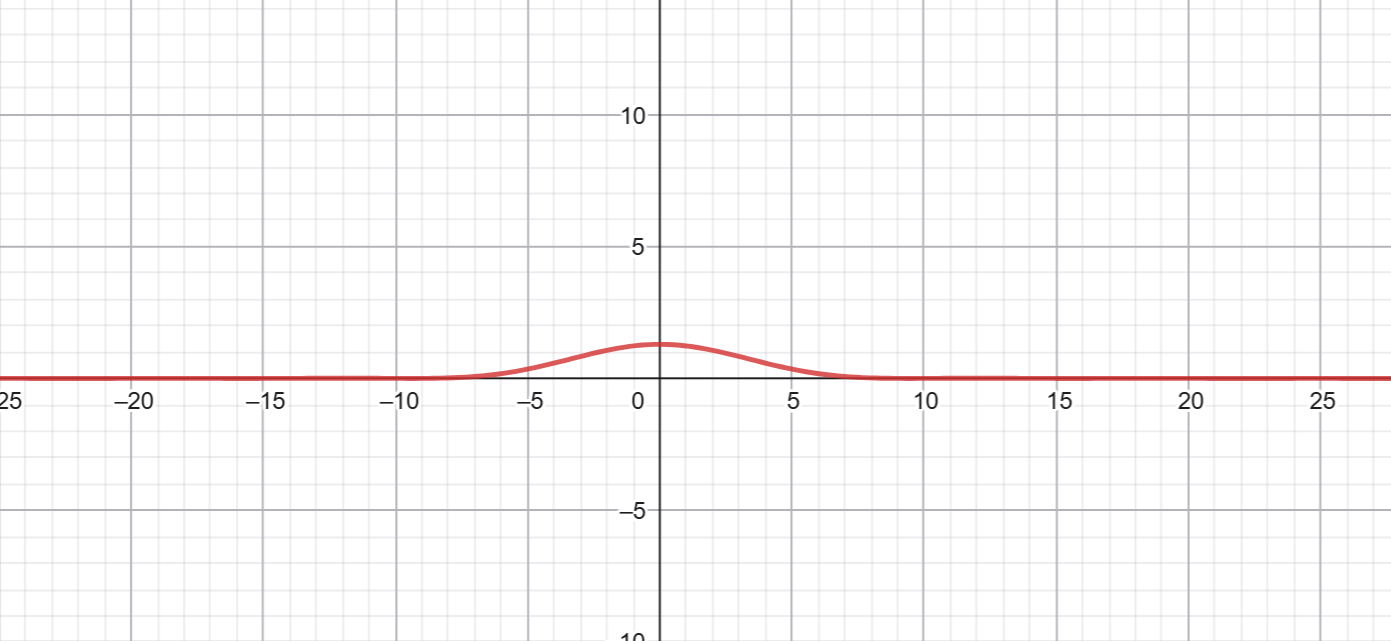
\includegraphics[width=0.8\textwidth,valign=t]{fig/prob3.34n1.png}
        \item $n=2$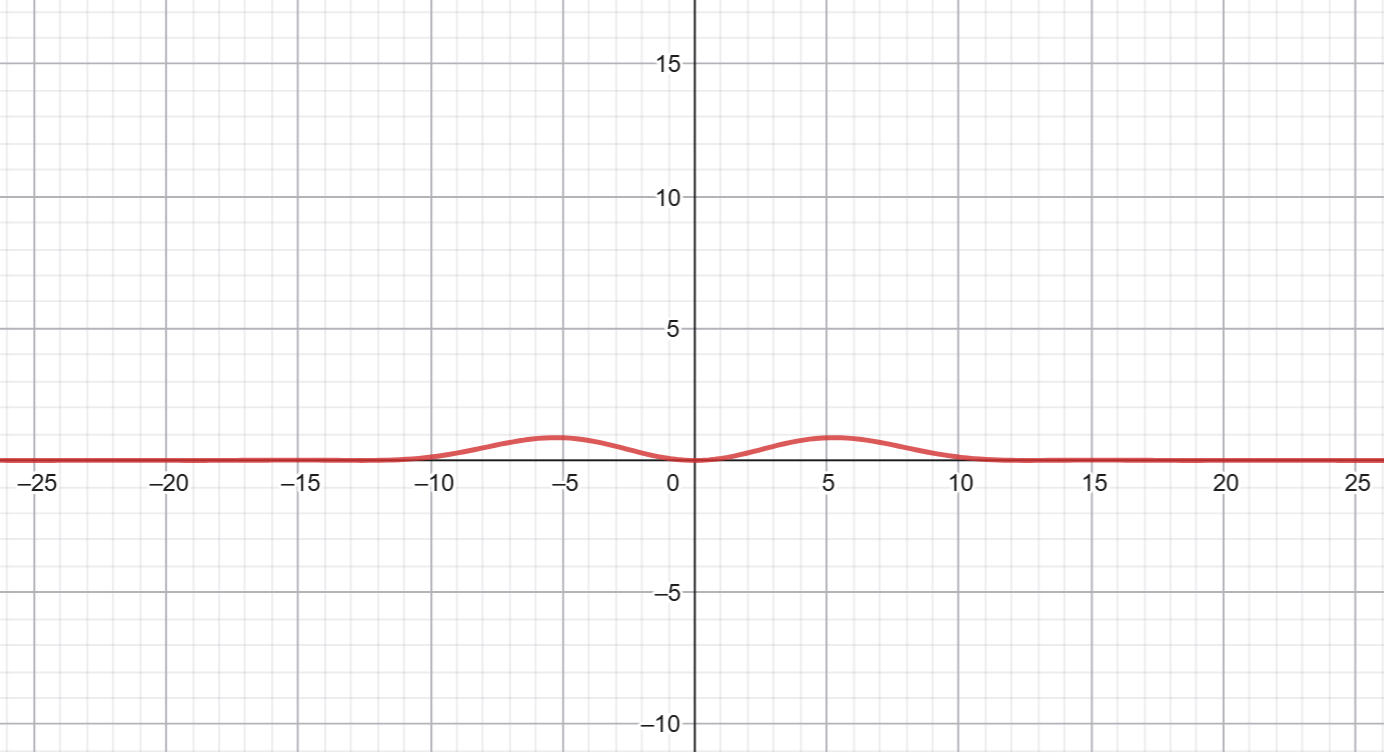
\includegraphics[width=0.8\textwidth, valign=t]{fig/prob3.34n2.png}
    \item $n=5$ 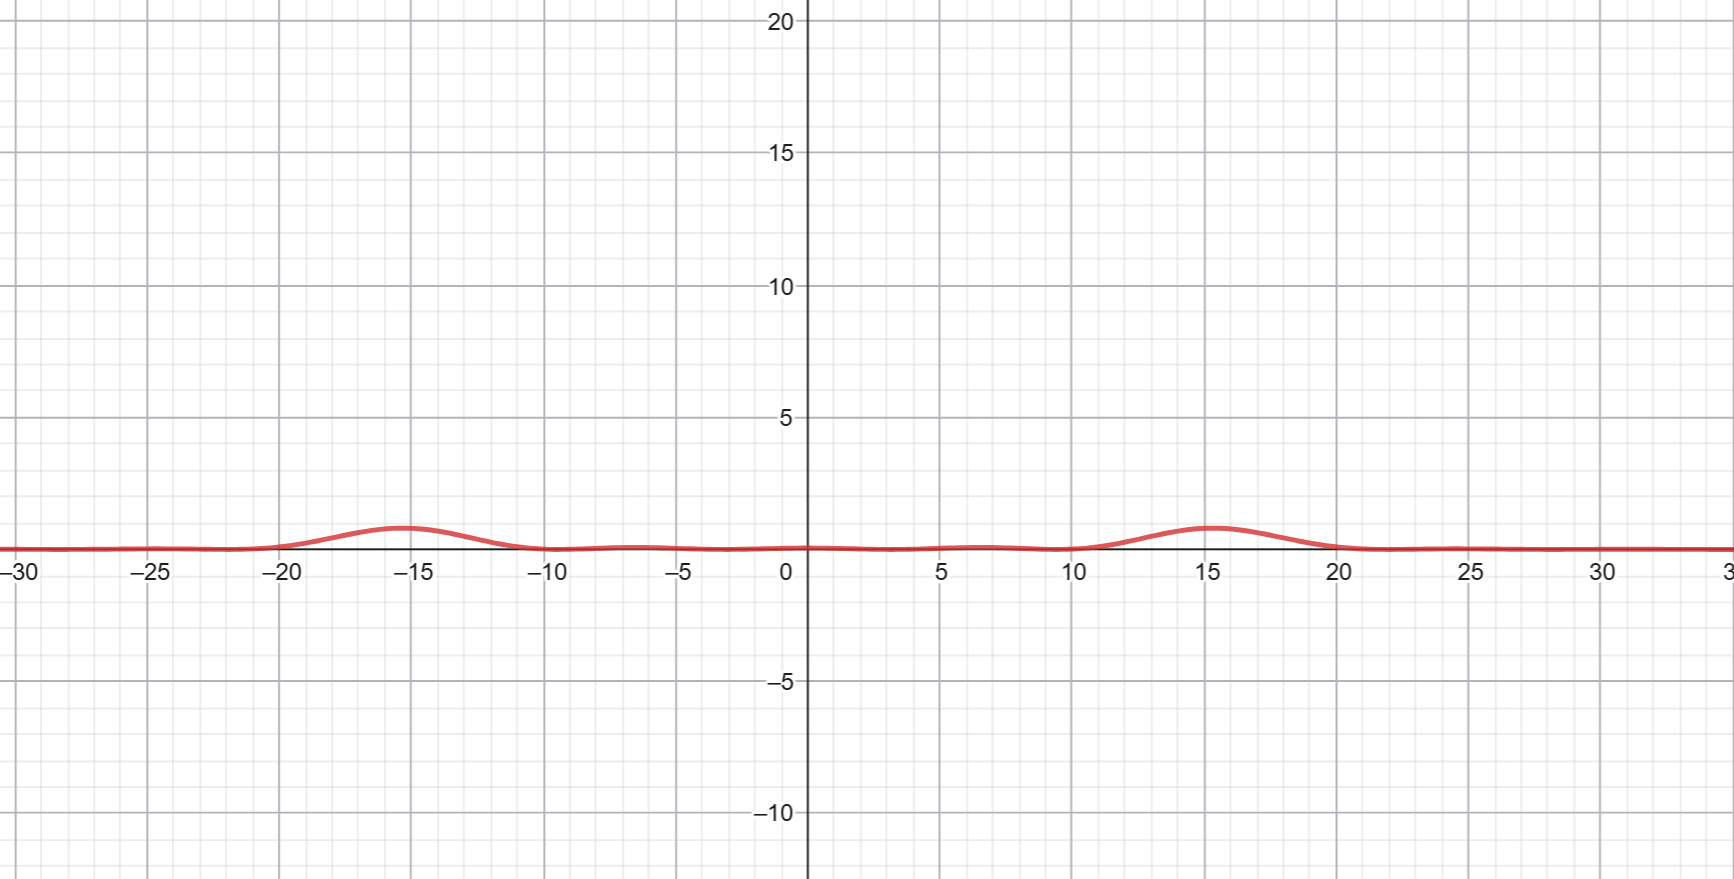
\includegraphics[width=0.8\textwidth, valign=t]{fig/prob3.34n5.png}
    \item $n=10$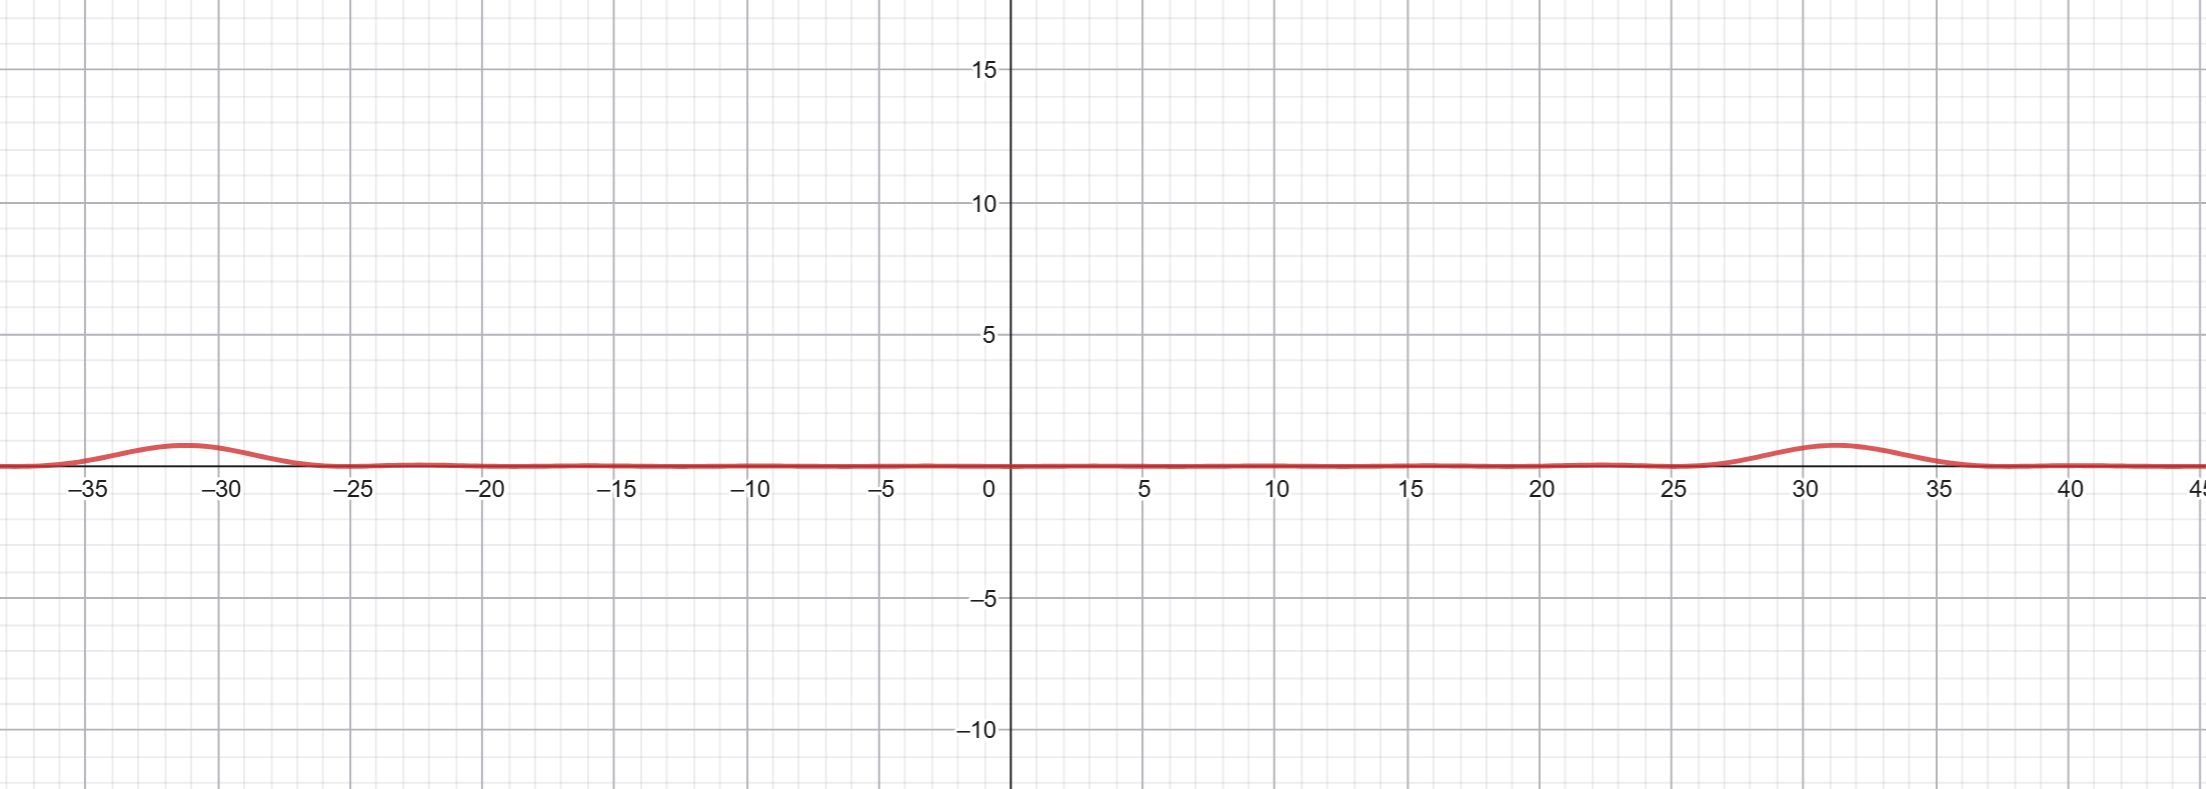
\includegraphics[width=0.8\textwidth, valign=t]{fig/prob3.34n10.png}
    \end{itemize}
    
    For large $n,$ the most probable values are $p=\pm\frac{n\pi\hbar}{a}.$

    For large $n,$ it behaves more like a classical particle. So $\frac{p^2}{2m}=E_n=\frac{n^2\pi^2\hbar^2}{2ma^2},$ the momentum is likely to be $\frac{n\pi\hbar}{a}.$ 

    In prob3.10, we observe that the ground state of the infinite square well is not an eigenvector of the momentum operator. However for large $n,$ the possible values concentrate on only two numbers, and the states, although not exactly, behave as if the eigenvectors of the momentum operator.

    \item 
    \begin{align*}
        \langle p^2\rangle=&
        \int_{-\infty}^{\infty} p^2\frac{1}{a\pi\hbar}
        \left(\frac{\pi n/a}{\pi^2n^2/a^2-p^2/\hbar^2}\right)^2
        2\left(1-(-1)^n\cos\frac{pa}{\hbar}\right) dp\\
        =&
        \frac{2}{a\pi\hbar}
        \frac{\pi^2n^2}{a^2}
        \int_{-\infty}^{\infty}
        \left(
        \frac{p}{\pi^2n^2/a^2-p^2/\hbar^2}
        \right)^2
        (1-(-1)^n\cos\frac{pa}{\hbar})dp
    \end{align*}
    This integration is far too complex. After doing some research, I confirmed that the result is as same as prob2.4, $\langle p^2\rangle=\frac{n^2\pi^2\hbar^2}{a^2}.$
    
\end{enumerate}

\subsection*{Sol. 35}
\begin{align*}
    \Phi(p,0)=&
    \frac{1}{\sqrt{2\pi\hbar}}
    \int_{-n\lambda}^{n\lambda}
    e^{-ipx/\hbar}
    \frac{1}{\sqrt{2n\lambda}}
    e^{i2\pi x/\lambda}dx
    \\=&
     \frac{1}{\sqrt{2\pi\hbar}}
     \frac{1}{\sqrt{2n\lambda}}
     \frac{1}{\frac{-ip}{\hbar}+\frac{2\pi i}{\lambda}}
     (e^{(2\pi i/\lambda-ip/\hbar)n\lambda}-e^{-(2\pi i/\lambda-ip/\hbar)n\lambda})\\
     =&\frac{1}{\sqrt{\pi\hbar n\lambda}}\frac{\lambda\hbar}{p\lambda-2\pi \hbar}\sin\left(\frac{pn\lambda}{\hbar}\right)
\end{align*}
\begin{align*}
    |\Psi(x,0)|^2 = \frac{1}{2n\lambda}, \; -n\lambda < x<n\lambda
\end{align*}
\begin{align*}
    |\Phi(p,0)|^2 = 
    \frac{1}{\pi n}\frac{\lambda\hbar}{(p\lambda-2\pi \hbar)^2}
    \sin^2\left(\frac{pn\lambda}{\hbar}\right)
\end{align*}
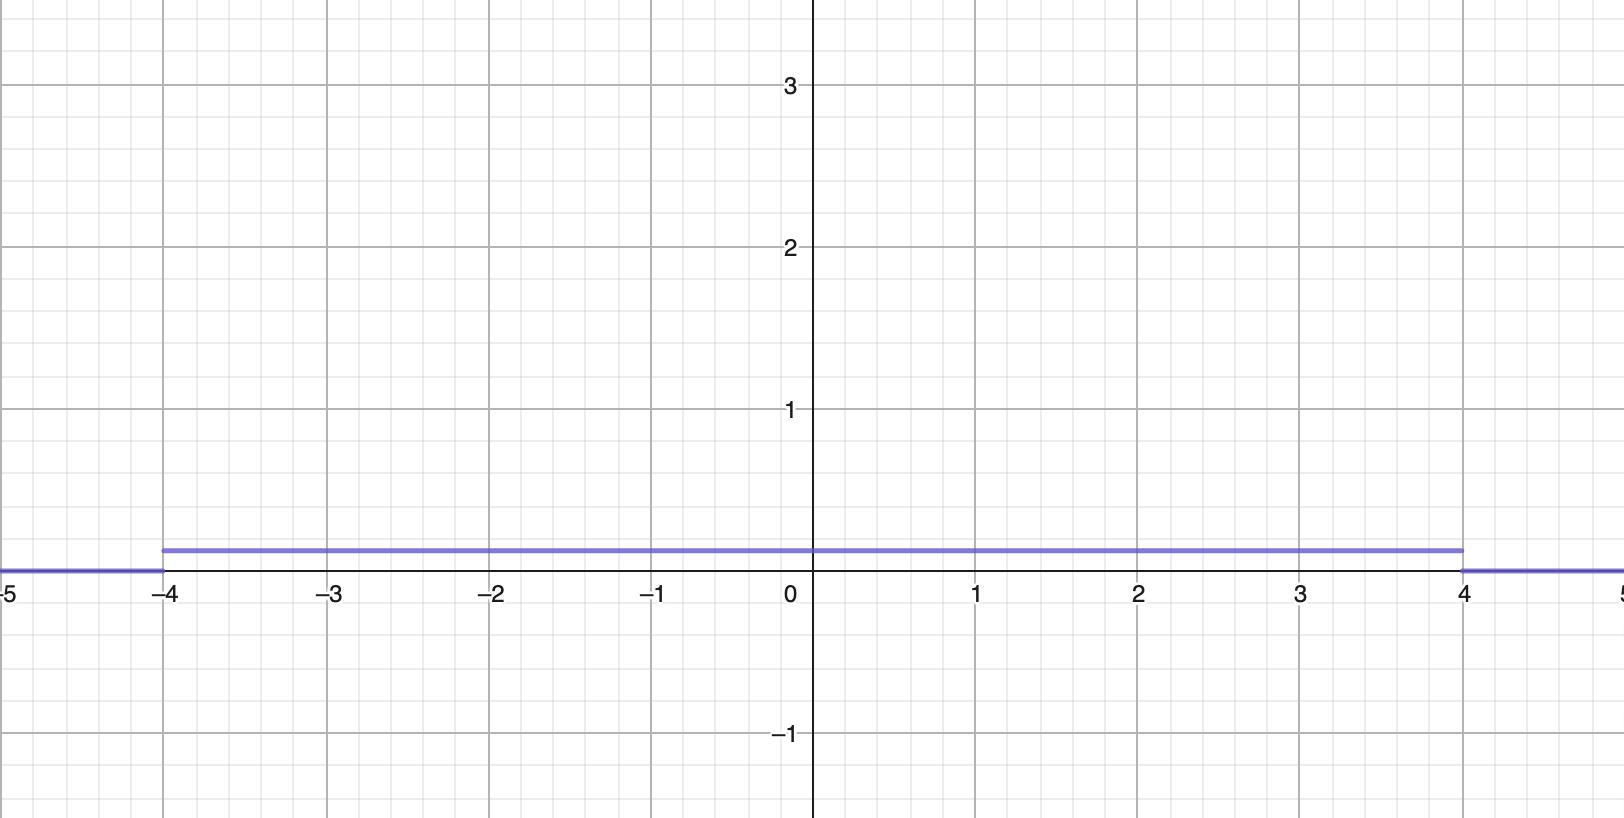
\includegraphics[width=0.8\textwidth, valign=t]{fig/prob3.35x.png}

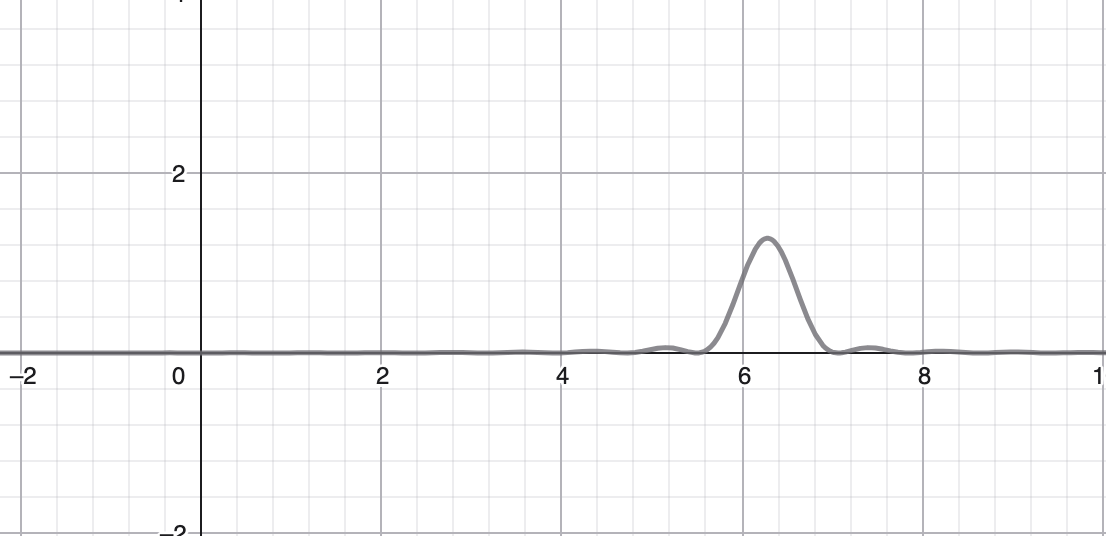
\includegraphics[width=0.8\textwidth, valign=t]{fig/prob3.35p.png}

$$
w_x = 2n\lambda
$$
$$
w_p = \frac{2\pi \hbar}{n\lambda}
$$
As $n\to\infty,$ $w_x\to\infty,$ $w_p\to0.$
$$
w_xw_p = 4\pi\hbar \geq \frac{\hbar}{2}
$$

\begin{align*}
    \langle p\rangle
=&\int_{-n\lambda}^{n\lambda}
\frac{1}{\sqrt{2n\lambda}}e^{-i2\pi x/\lambda}
(-i\hbar\frac{d}{dx})
\frac{1}{\sqrt{2n\lambda}}e^{i2\pi x/\lambda}dx\\
=&\frac{-i\hbar}{2n\lambda}
\int_{-n\lambda}^{n\lambda}
e^{-i2\pi x/\lambda}(i2\pi/\lambda)e^{i2\pi x/\lambda}dx\\
=&\frac{2\pi\hbar}{\lambda}
\end{align*}

\begin{align*}
    \langle p^2\rangle
=&\int_{-n\lambda}^{n\lambda}
\frac{1}{\sqrt{2n\lambda}}e^{-i2\pi x/\lambda}
(-\hbar^2\frac{d^2}{dx^2})
\frac{1}{\sqrt{2n\lambda}}e^{i2\pi x/\lambda}dx\\
=&\frac{-\hbar^2}{2n\lambda}
\int_{-n\lambda}^{n\lambda}
e^{-i2\pi x/\lambda}(i2\pi/\lambda)^2e^{i2\pi x/\lambda}dx\\
=&\frac{4\pi^2\hbar^2}{\lambda^2}
\end{align*}

$\sigma_p=0.$ The abrupt cutoff at the endpoints makes this result not reliable. It hides a delta function when momentum operator is applied.

\subsection*{Sol. 36}
\begin{enumerate}
    \item 
    \begin{align*}
        \int_{-\infty}^{\infty}
        \frac{A^2}{(x^2+a^2)^2}dx = \frac{\pi A^2}{2a^3}.
    \end{align*}
    $$
    A = \sqrt{\frac{2a^3}{\pi}}.
    $$
    \item 
    \begin{align*}
        \langle x\rangle
        =
        \frac{2a^3}{\pi}\int_{-\infty}^{\infty} \frac{x}{(x^2+a^2)^2}dx=0
    \end{align*}
    \begin{align*}
        \langle x^2\rangle
        =
        \frac{2a^3}{\pi}\int_{-\infty}^{\infty} \frac{x^2}{(x^2+a^2)^2}dx=a
    \end{align*}
    $$
    \sigma_x=\sqrt{a}
    $$
    \item 
    \begin{align*}
        \Phi(p,0)
        =&
        \frac{1}{\sqrt{2\pi\hbar}}
        \int_{-\infty}^{\infty}
        e^{-ipx/\hbar}
        \sqrt{\frac{2a^3}{\pi}}
        \frac{1}{x^2+a^2}dx\\
        =&\sqrt{\frac{a}{\hbar}}e^{-\frac{a|p|}{\hbar}}
    \end{align*}
    \begin{align*}
        \int_{-\infty}^{\infty}
        \frac{a}{\hbar}e^{-\frac{2a|p|}{\hbar}}dp = 1
    \end{align*}
    \item 
    \begin{align*}
        \langle p\rangle
        =\int_{-\infty}^{\infty}
        \frac{a}{\hbar}pe^{-\frac{2a|p|}{\hbar}}dp= 0
    \end{align*}
    \begin{align*}
        \langle p^2\rangle
        =\int_{-\infty}^{\infty}
        \frac{a}{\hbar}p^2e^{-\frac{2a|p|}{\hbar}}dp= \frac{\hbar^2}{2a^2}
    \end{align*}
    $$
    \sigma_p = \frac{\hbar}{\sqrt{2}a}
    $$
    \item 
    $$
    \sigma_x\sigma_p=\frac{\hbar}{\sqrt{2}}\geq \frac{\hbar}{2}
    $$
\end{enumerate}

\subsection*{Sol. 37}
\begin{align*}
    \frac{d}{dt}\langle xp\rangle
    =&\frac{i}{\hbar}
    \langle[H,xp]\rangle\\
    =&\frac{i}{\hbar}
    \langle[T+V,xp]\rangle\\
    =&\frac{i}{\hbar}
    \langle x[V,p]+[T,x]p\rangle)\\
    =&\frac{i}{\hbar}
    \langle i\hbar x\frac{\partial V}{\partial x}+\frac{-i\hbar}{m}p^2\rangle\\
    =&2\langle T\rangle-\langle x\frac{\partial V}{\partial x}\rangle.
\end{align*}
There is no $t$ term in the stationary state, so
$$
2\langle T\rangle=\langle x\frac{d V}{d x}\rangle.
$$
For a harmonic oscillator, $V=\frac{1}{2}m\omega^2x^2,$
$$
2\langle T \rangle = \langle xm\omega^2x\rangle\Rightarrow
\langle T\rangle=\langle V\rangle.
$$

\subsection*{Sol. 38}
$$
\Psi(x,t) = 
\frac{1}{\sqrt{2}}\psi_1(x)e^{-iE_1t/\hbar} +
\frac{1}{\sqrt{2}}\psi_2(x)e^{-iE_2t/\hbar}
$$

\begin{align*}
    &\int 
    \left(\frac{1}{\sqrt{2}}\psi_1(x) +
\frac{1}{\sqrt{2}}\psi_2(x)\right)
    \left(\frac{1}{\sqrt{2}}\psi_1(x)e^{-iE_1\tau/\hbar} +
\frac{1}{\sqrt{2}}\psi_2(x)e^{-iE_2\tau/\hbar}\right)dx\\
=&
\frac{1}{2}e^{-iE_1\tau/\hbar}
+\frac{1}{2}e^{-iE_2\tau/\hbar}=0
\end{align*}
$$
\frac{E_2\tau}{\hbar}-\frac{E_1\tau}{\hbar}=\pi 
\Rightarrow\tau=\frac{\pi\hbar}{E_2-E_1}
$$

$$
\Delta H = \sqrt{\frac{1}{2}(E_1^2+E_2^2)-\frac{1}{4}(E_1+E_2)^2}
$$

$$
\Delta H\Delta t
=
\hbar\sqrt{\frac{\frac{1}{2}(E_1^2+E_2^2)-\frac{1}{4}(E_1+E_2)^2}{(E_2-E_1)^2}} = \frac{\hbar}{2}
$$
\subsection*{Sol. 39}

\begin{align*}
    \langle n,xn'\rangle
    =& \left\langle \frac{1}{\sqrt{n!}}
    a_+^n\psi_0,
    x\frac{1}{\sqrt{n'!}}a_+^{n'}\psi_0\right\rangle\\
    =&
    \frac{1}{\sqrt{n!}}
    \frac{1}{\sqrt{n'!}}
    \sqrt{\frac{\hbar}{2m\omega}}
    \langle \psi_0, (a_-)^{n}(a_++a_-)(a_+)^{n'}\psi_0\rangle\\
    =&\frac{1}{\sqrt{n!}}
    \frac{1}{\sqrt{n'!}}
    \sqrt{\frac{\hbar}{2m\omega}}
    (\langle \psi_0, (a_-)^{n}(a_+)^{n'+1}\psi_0\rangle
    +\langle \psi_0, (a_-)^{n+1}(a_+)^{n'}\psi_0\rangle
    )\\
    =&\sqrt{\frac{\hbar}{2m\omega}}(\sqrt{n}\delta_{n-1,n'}+\sqrt{n'}\delta_{n,n'-1})
\end{align*}


\begin{align*}
    \langle n,pn'\rangle
    =& \left\langle \frac{1}{\sqrt{n!}}
    a_+^n\psi_0,
    p\frac{1}{\sqrt{n'!}}a_+^{n'}\psi_0\right\rangle\\
    =&
    \frac{1}{\sqrt{n!}}
    \frac{1}{\sqrt{n'!}}
    i\sqrt{\frac{\hbar m\omega}{2}}
    \langle \psi_0, (a_-)^{n}(a_+-a_-)(a_+)^{n'}\psi_0\rangle\\
    =&\frac{1}{\sqrt{n!}}
    \frac{1}{\sqrt{n'!}}
    i\sqrt{\frac{\hbar m\omega}{2}}
    (\langle \psi_0, (a_-)^{n}(a_+)^{n'+1}\psi_0\rangle
    -\langle \psi_0, (a_-)^{n+1}(a_+)^{n'}\psi_0\rangle
    )\\
    =& i\sqrt{\frac{\hbar m\omega}{2}}(\sqrt{n}\delta_{n-1,n'}-\sqrt{n'}\delta_{n,n'-1})
\end{align*}


\begin{align*}
    X^2_{jk} =&
    \sum_{l}X_{jl}X_{lk}\\
    =&\frac{\hbar}{2m\omega}
    \sum_{l}
    (\sqrt{j}\delta_{j-1,l}+\sqrt{l}\delta_{j,l-1})
    (\sqrt{l}\delta_{l-1,k}+\sqrt{k}\delta_{l,k-1})\\
    =&\frac{\hbar}{2m\omega}
    (\sqrt{j}
    (\sqrt{j-1}\delta_{j-1,k}+
    \sqrt{k}\delta_{j-1,k-1})
    +
    \sqrt{j+1}
    (\sqrt{j+1}\delta_{j,k}+
    \sqrt{k}\delta_{j+1,k-1})\\
    &+
    (\sqrt{j}\delta_{j-1,k+1}+
    \sqrt{k+1}\delta_{j,k})\sqrt{k+1}+
    (\sqrt{j}\delta_{j-1,k-1}+
    \sqrt{k-1}\delta_{j,k-2})\sqrt{k}
    )
\end{align*}
\begin{align*}
    P^2_{jk} =&
    \sum_{l}P_{jl}P_{lk}\\
    =&-\frac{\hbar m\omega}{2}
    \sum_{l}
    (\sqrt{j}\delta_{j-1,l}-\sqrt{l}\delta_{j,l-1})
    (\sqrt{l}\delta_{l-1,k}-\sqrt{k}\delta_{l,k-1})\\
    =&-\frac{\hbar m\omega}{2}
    (\sqrt{j}
    (\sqrt{j-1}\delta_{j-1,k}-
    \sqrt{k}\delta_{j-1,k-1})
    -
    \sqrt{j+1}
    (\sqrt{j+1}\delta_{j,k}-
    \sqrt{k}\delta_{j+1,k-1})\\
    &+
    (\sqrt{j}\delta_{j-1,k+1}-
    \sqrt{k+1}\delta_{j,k})\sqrt{k+1}-
    (\sqrt{j}\delta_{j-1,k-1}-
    \sqrt{k-1}\delta_{j,k-2})\sqrt{k}
    )
\end{align*}

\begin{align*}
    \frac{1}{2m}P^2_{jk}
    +\frac{m\omega^2}{2}X^2_{jk}
    =&\frac{\hbar\omega}{4}
    2(\sqrt{kj}\delta_{j,k}+(j+1)\delta_{j,k}+(k+1)\delta_{j,k}+\sqrt{jk}\delta_{j,k})\\
    =&\frac{\hbar\omega}{2}(2j+1)\delta_{j,k}
\end{align*}

\subsection*{Sol. 40}
\begin{align*}
    \langle x\rangle = &
    \sum_{n,s}c_s^*e^{iE_nt/\hbar}
    c_ne^{-iE_st/\hbar}\langle\psi_s, x\psi_n\rangle\\
    =&\sqrt{\frac{\hbar}{2m\omega}}\sum_{n,s}
    c_s^*c_ne^{iE_nt/\hbar}
    e^{-iE_st/\hbar}(\sqrt{n}\delta_{s,n-1}+\sqrt{s}\delta_{s-1,n})\\
    =&\sqrt{\frac{\hbar}{2m\omega}}\sum_n(
    c_{n+1}^*c_ne^{iE_nt/\hbar}
    e^{-iE_{n+1}t/\hbar}\sqrt{n+1}
    +c_{n-1}^*c_ne^{iE_nt/\hbar}
    e^{-iE_{n-1}t/\hbar}\sqrt{n})\\
    =&\sqrt{\frac{\hbar}{2m\omega}}\sum_n
    \sqrt{n+1}
    (c^*_{n+1}c_ne^{-i\omega t}+c^*_{n}c_{n+1}e^{i\omega t})
\end{align*}
Let $$
Ce^{i\phi} = 
\sqrt{\frac{2\hbar}{m\omega}}\sum_n
    \sqrt{n+1}
    c^*_{n+1}c_n,
$$ then 
$$
\langle x\rangle
=\frac{1}{2}Ce^{i\phi}e^{-i\omega t} + \frac{1}{2}Ce^{-i\phi} e^{i\omega t} = C\cos(\omega t-\phi).
$$

For problem 2.40, $c_0=\frac{3}{5},$ $c_1=-\frac{2\sqrt{2}}{5},$ $c_2=\frac{2\sqrt{2}}{5}.$
$$
\phi=0,
$$
$$
C = \sqrt{\frac{2\hbar}{m\omega}}
(\sqrt{1}c_1c_0+\sqrt{2}c_2c_1)
= \sqrt{\frac{2\hbar}{m\omega}}
(-\frac{14\sqrt{2}}{25}).
$$


\subsection*{Sol. 41}
$$
\Psi(x,t) = \frac{1}{\sqrt{2}}\psi_0e^{-iE_0t/\hbar}
+
\frac{1}{\sqrt{2}}\psi_1e^{-iE_1t/\hbar}
$$

\begin{align*}
    \langle p\rangle =& 
    \langle \frac{1}{\sqrt{2}}\psi_0e^{-iE_0t/\hbar}
+
\frac{1}{\sqrt{2}}\psi_1e^{-iE_1t/\hbar}, p(\frac{1}{\sqrt{2}}\psi_0e^{-iE_0t/\hbar}
+
\frac{1}{\sqrt{2}}\psi_1e^{-iE_1t/\hbar})\rangle\\
=&\frac{1}{2}e^{iE_0 t/\hbar}e^{-iE_1 t/\hbar}\langle \psi_0, p\psi_1\rangle
+\frac{1}{2}e^{-iE_0 t/\hbar}e^{iE_1 t/\hbar}\langle \psi_1, p\psi_0\rangle\\
=&
\frac{1}{2}e^{iE_0 t/\hbar}e^{-iE_1 t/\hbar}
(-i\sqrt{\frac{\hbar m\omega}{2}})
+\frac{1}{2}e^{-iE_0 t/\hbar}e^{iE_1 t/\hbar} 
(i\sqrt{\frac{\hbar m\omega}{2}})\\
=&-\sqrt{\frac{\hbar m\omega}{2}}\sin\omega t
\end{align*}
The largest value of $\langle p\rangle$ is $\sqrt{\frac{\hbar m\omega}{2}}.$

\subsection*{Sol. 42}
\begin{enumerate}
    \item 
    \begin{align*}
        \langle x\rangle
        =&
        \sqrt{\frac{\hbar}{2m\omega}}
        \langle \alpha, (a_++a_-)\alpha\rangle\\
        =&\sqrt{\frac{\hbar}{2m\omega}}
        (\langle a_-\alpha,\alpha\rangle + \langle\alpha,a_-,\alpha\rangle)\\
        =&
        \sqrt{\frac{\hbar}{2m\omega}}
        (\bar{\alpha}+\alpha)
    \end{align*}
    \begin{align*}
        \langle x^2\rangle
        =&
        \frac{\hbar}{2m\omega}
        \langle \alpha, (a_++a_-)^2\alpha\rangle\\
        =&\frac{\hbar}{2m\omega}
        (\langle\alpha, a_+^2\alpha\rangle+
        \langle\alpha, a_+a_-\alpha\rangle
        +
        \langle\alpha, a_-a_+\alpha\rangle+
        \langle\alpha, a_-^2\alpha\rangle)\\
        =&\frac{\hbar}{2m\omega}
        (\langle a_-^2\alpha, \alpha\rangle+
        \langle a_-\alpha, a_-\alpha\rangle
        +
        \langle\alpha, (1+a_+a_-)\alpha\rangle+
        \langle\alpha, a_-^2\alpha\rangle)\\
        =&
        \frac{\hbar}{2m\omega}
        (\bar{\alpha}^2+\alpha^2+2\bar{\alpha}\alpha + 1
        )
    \end{align*}
    \begin{align*}
        \langle p\rangle
        =&
        i
        \sqrt{\frac{\hbar m\omega}{2}}
        \langle \alpha, (a_+-a_-)\alpha\rangle\\
        =&i
        \sqrt{\frac{\hbar m\omega}{2}}
        (\langle a_-\alpha,\alpha\rangle -\langle\alpha,a_-,\alpha\rangle)\\
        =&
        i
        \sqrt{\frac{\hbar m\omega}{2}}
        (\bar{\alpha}-\alpha)
    \end{align*}
    \begin{align*}
        \langle p^2\rangle
        =&
        -\frac{\hbar m\omega}{2}
        \langle \alpha, (a_+-a_-)^2\alpha\rangle\\
        =&-\frac{\hbar m\omega}{2}
        (\langle\alpha, a_+^2\alpha\rangle-
        \langle\alpha, a_+a_-\alpha\rangle
        -
        \langle\alpha, a_-a_+\alpha\rangle+
        \langle\alpha, a_-^2\alpha\rangle)\\
        =&-\frac{\hbar m\omega}{2}
        (\langle a_-^2\alpha, \alpha\rangle
        -
        \langle a_-\alpha, a_-\alpha\rangle
        -
        \langle\alpha, (1+a_+a_-)\alpha\rangle+
        \langle\alpha, a_-^2\alpha\rangle)\\
        =&
        -\frac{\hbar m\omega}{2}
        (\bar{\alpha}^2-2\bar{\alpha}\alpha - 1 + \alpha^2
        )
    \end{align*}
    \item 
    $$
    \sigma_x= 
    \sqrt{\frac{\hbar}{2m\omega}}
    $$
    $$
    \sigma_p = 
    \sqrt{\frac{\hbar m\omega}{2}}
    $$
    $$
    \sigma_x\sigma_p=\frac{\hbar}{2}
    $$
    \item 
    $$
    \sum_{n=0}c_na_-| n\rangle = 
    \sum_{n=0}c_n\sqrt{n}|n-1\rangle
    =
    \sum_{n=0}c_{n+1}\sqrt{n+1}|n\rangle
    =\alpha\sum_{n=0}c_n| n\rangle
    $$
    Thus, $$c_{n+1}\sqrt{n+1}=\alpha c_n
    \Rightarrow
    c_n = \frac{\alpha^n}{\sqrt{n!}}c_0.
    $$ 
    \item 
    \begin{align*}
        \sum_{n=0}\frac{|\alpha|^{2n}}{n!}|c_0|^2=
        |c_0|^2e^{|\alpha|^2}\Rightarrow c_0=e^{-|\alpha|^2/2}\\
    \end{align*}
    \item 
    \begin{align*}
        a_-|\alpha(t)\rangle =&
        a_-\sum_{n=0} \frac{\alpha^n}{\sqrt{n!}}c_0e^{-i\omega(2n+1)t/2}|n\rangle\\
        =&\sum_{n=1} \frac{\alpha^n}{\sqrt{(n-1)!}}c_0e^{-i\omega(2n+1)t/2}|n-1\rangle
        \\
        =&\sum_{n=0} \frac{\alpha^{n+1}}{\sqrt{n!}}c_0e^{-i\omega(2n+3)t/2}|n\rangle\\
        =&\alpha e^{-i\omega t}|\alpha(t)\rangle
    \end{align*}
    \item 
    \begin{align*}
        \langle x\rangle
        =&\sqrt{\frac{\hbar}{2m\omega}}
        (e^{i\omega t}\bar{\alpha} + e^{-i\omega t}\alpha)\\
        =&C\cos(\omega t-\phi)
    \end{align*}
    $$
    \sigma_x = \sqrt{\frac{\hbar}{2m\omega}}
    $$
    \item 
    Yes. Since $a_-\psi_0=0\cdot\psi_0,$ the eigenvalue is 0.
\end{enumerate}

\subsection*{Sol. 43}
\begin{enumerate}
    \item 
    By equation 3.59, 
    $$
    \sigma_A^2\sigma_B^2\geq |\langle AB\rangle-\langle A\rangle\langle B\rangle|^2
    $$

    \begin{align*}
        \frac{1}{4}(\langle C\rangle^2+\langle D\rangle^2)
    =&
    \frac{1}{4}
    (\langle -i(AB-BA)\rangle^2 + \langle AB+BA-2\langle A\rangle\langle B\rangle\rangle^2)\\
    =&
    \frac{1}{4}
    (\langle -i(AB-BA)\rangle^2 + \langle AB+BA-2\langle A\rangle\langle B\rangle\rangle^2)\\
    =&
    \frac{1}{4}
    (-\langle AB\rangle^2+2\langle AB\rangle\langle BA\rangle
    -\langle BA\rangle^2
    + \langle AB\rangle^2 
    + \langle BA\rangle^2\\
    &+ 4\langle A\rangle^2\langle B\rangle^2
    + 2\langle AB\rangle\langle BA\rangle
    -2\langle AB\rangle\langle A\rangle\langle B\rangle
    -2\langle BA\rangle\langle A\rangle\langle B\rangle
    )\\
    =&
    \frac{1}{4}(4\langle AB\rangle\langle BA\rangle+
    4\langle A\rangle^2\langle B\rangle^2
    -2\langle AB\rangle\langle A\rangle\langle B\rangle
    -2\langle BA\rangle\langle A\rangle\langle B\rangle
    )\\
    =&|\langle AB\rangle-\langle A\rangle\langle B\rangle|^2
    \end{align*}
    \item If $B=A,$ then
    $$
    \sigma_A^4\geq 
    \frac{1}{4}(\langle 2A^2-2\langle A\rangle^2\rangle^2)
    \Rightarrow 
    \sigma_A^2\geq 
    \langle A^2-\langle A\rangle^2\rangle
    \Rightarrow \sigma_A^2\geq \sigma_A^2.
    $$
\end{enumerate}

\subsection*{Sol. 44}
\begin{enumerate}
    \item 
    \begin{align*}
        det(H-tI)=&
    (a-t)(c-t)(a-t) - b^2(c-t)\\
    =&(c-t)(a^2-2at+t^2-b^2)\\
    =&(c-t)(a+b-t)(a-b-t)
    \end{align*}
    Eigenvalues $c: 
    \begin{pmatrix}
    0\\1\\ 0
    \end{pmatrix},
    $
    $a+b: 
    \frac{1}{\sqrt{2}}\begin{pmatrix}
    1\\0\\ 1
    \end{pmatrix},
    $
    $a-b: 
    \frac{1}{\sqrt{2}}
    \begin{pmatrix}
    1\\0\\ -1
    \end{pmatrix}.
    $

    If $|\mathcal{S}(0)\rangle = \begin{pmatrix}
        0\\1\\0
    \end{pmatrix},$ then
    $$
    |\mathcal{S}(t)\rangle
    =
    \begin{pmatrix}
    0\\1\\ 0
    \end{pmatrix}e^{-ict/\hbar}
    $$
    \item 

     If $|\mathcal{S}(0)\rangle = \begin{pmatrix}
        1\\0\\0
    \end{pmatrix},$ then
    $$
    |\mathcal{S}(t)\rangle
    =
    \frac{1}{2}
    \begin{pmatrix}
    1\\0\\ 1
    \end{pmatrix}e^{-i(a+b)t/\hbar}
    +
    \frac{1}{2}
    \begin{pmatrix}
    1\\0\\ -1
    \end{pmatrix}e^{-i(a-b)t/\hbar}.
    $$
    
\end{enumerate}

\subsection*{Sol. 45}
\begin{align*}
    \langle n|\hat{x}|\mathcal{S}(t)\rangle =& 
    \sum_{n'}\langle n|\hat{x}|n'\rangle\langle n'|\mathcal{S}(t)\rangle \\
    =& 
    \sum_{n'}c_{n'}(t)\langle n|\hat{x}|n'\rangle\\
    =&\sqrt{\frac{\hbar}{2m\omega}}
    \sum_{n'}
    c_{n'}(t)
    (\sqrt{n'}\delta_{n,n'-1}
    +\sqrt{n}\delta_{n',n-1}
    )\\
    =&
    \sqrt{\frac{\hbar}{2m\omega}}
    (c_{n+1}(t)\sqrt{n+1}
    +
    c_{n-1}(t)\sqrt{n}
    )
\end{align*}
\subsection*{Sol. 46}

\begin{enumerate}
    \item 
    $H:$
    Eigenvalues: 
    \begin{itemize}
        \item $
    \hbar\omega: 
    \begin{pmatrix}
    1\\0\\0
    \end{pmatrix}
    $
     \item $
    2\hbar\omega: 
    \begin{pmatrix}
    0\\1\\0
    \end{pmatrix}
    $
     \item $
    2\hbar\omega: 
    \begin{pmatrix}
    0\\0\\1
    \end{pmatrix}
    $
    \end{itemize}

     $A:$
    Eigenvalues: 
    \begin{itemize}
        \item $
    2\lambda: 
    \begin{pmatrix}
    0\\0\\1
    \end{pmatrix}
    $
     \item $
    \lambda:
    \frac{1}{\sqrt{2}}
    \begin{pmatrix}
    1\\1\\0
    \end{pmatrix}
    $
     \item $
    -\lambda: 
    \frac{1}{\sqrt{2}}
    \begin{pmatrix}
    1\\-1\\0
    \end{pmatrix}
    $
    
    \end{itemize}
    $B:$
    Eigenvalues: 
    \begin{itemize}
        \item $
    2\mu: 
    \begin{pmatrix}
    1\\0\\0
    \end{pmatrix}
    $
     \item $
    \mu: 
    \frac{1}{\sqrt{2}}
    \begin{pmatrix}
    0\\1\\1
    \end{pmatrix}
    $
     \item $
    -\mu: 
    \frac{1}{\sqrt{2}}
    \begin{pmatrix}
    0\\1\\-1
    \end{pmatrix}
    $
    
    \end{itemize}

    \item 
    $$
    \langle H\rangle
    =
    \begin{pmatrix}
        c_1^* & 
        c_2^* & 
        c_3^*
    \end{pmatrix}
    \hbar\omega
    \begin{pmatrix}
        1 & 0 & 0\\
        0 & 2 & 0\\
        0 & 0 & 2
    \end{pmatrix}
    \begin{pmatrix}
        c_1\\c_2\\c_3
    \end{pmatrix}
    =\hbar\omega
    (|c_1|^2+2|c_2|^2+2|c_3|^2)
    $$
    $$
    \langle A\rangle
    =
    \begin{pmatrix}
        c_1^* & 
        c_2^* & 
        c_3^*
    \end{pmatrix}
    \lambda
    \begin{pmatrix}
        0 & 1 & 0\\
        1 & 0 & 0\\
        0 & 0 & 2
    \end{pmatrix}
    \begin{pmatrix}
        c_1\\c_2\\c_3
    \end{pmatrix}
    =\lambda
    (c_1^*c_2 + c_2^*c_1+2|c_3|^2)
    $$
    $$
    \langle B\rangle
    =
    \begin{pmatrix}
        c_1^* & 
        c_2^* & 
        c_3^*
    \end{pmatrix}
    \mu
    \begin{pmatrix}
        2 & 0 & 0\\
        0 & 0 & 1\\
        0 & 1 & 0
    \end{pmatrix}
    \begin{pmatrix}
        c_1\\c_2\\c_3
    \end{pmatrix}
    =\mu
    (2|c_1|^2+c_2^*c_3+c_3^*c_2)
    $$
    \item 
    $$
    |\mathcal{S}
    (t)
    \rangle
    =
    c_1
    \begin{pmatrix}
        1\\0\\0
    \end{pmatrix}
    e^{-i\omega t}
    +
    c_2
    \begin{pmatrix}
        0\\1\\0
    \end{pmatrix}
    e^{-i2\omega t}
    +
    c_3
    \begin{pmatrix}
        0\\0\\1
    \end{pmatrix}
    e^{-i2\omega t}
    $$

    Measuring $H$ will get $\hbar\omega$ with probability $|c_1|^2,$ and $2\hbar\omega$ with probability $|c_2|^2+|c_3|^2.$

    \begin{align*}
        \langle \mathcal{S}(t)|A|\mathcal{S}(t)\rangle
        =& 
        \left[
         c_1^*
    \begin{pmatrix}
        1&0&0
    \end{pmatrix}
    e^{i\omega t}
    +
    c_2^*
    \begin{pmatrix}
        0&1&0
    \end{pmatrix}
    e^{i2\omega t}
    +
    c_3^*
    \begin{pmatrix}
        0&0&1
    \end{pmatrix}
    e^{i2\omega t}
    \right]
    \lambda
    \begin{pmatrix}
        0 & 1 & 0\\
        1 & 0 & 0\\
        0 & 0 & 2
    \end{pmatrix}\\
    &\left[
    c_1
    \begin{pmatrix}
        1\\0\\0
    \end{pmatrix}
    e^{-i\omega t}
    +
    c_2
    \begin{pmatrix}
        0\\1\\0
    \end{pmatrix}
    e^{-i2\omega t}
    +
    c_3
    \begin{pmatrix}
        0\\0\\1
    \end{pmatrix}
    e^{-i2\omega t}
    \right]\\
    =&
    \left[
         c_1^*
    \begin{pmatrix}
        1&0&0
    \end{pmatrix}
    e^{i\omega t}
    +
    c_2^*
    \begin{pmatrix}
        0&1&0
    \end{pmatrix}
    e^{i2\omega t}
    +
    c_3^*
    \begin{pmatrix}
        0&0&1
    \end{pmatrix}
    e^{i2\omega t}
    \right]
    \lambda
    \\
    &\left[
    c_1
    \begin{pmatrix}
        0\\1\\0
    \end{pmatrix}
    e^{-i\omega t}
    +
    c_2
    \begin{pmatrix}
        1\\0\\0
    \end{pmatrix}
    e^{-i2\omega t}
    +
    c_3
    \begin{pmatrix}
        0\\0\\2
    \end{pmatrix}
    e^{-i2\omega t}
    \right]\\
    =&\lambda(c_1^*c_2e^{-i\omega t}
    +c_2^*c_1e^{i\omega t}
    +|c_3|^2)
    \end{align*}

    \begin{align*}
        \langle \mathcal{S}(t)|B|\mathcal{S}(t)\rangle
        =& 
        \left[
         c_1^*
    \begin{pmatrix}
        1&0&0
    \end{pmatrix}
    e^{i\omega t}
    +
    c_2^*
    \begin{pmatrix}
        0&1&0
    \end{pmatrix}
    e^{i2\omega t}
    +
    c_3^*
    \begin{pmatrix}
        0&0&1
    \end{pmatrix}
    e^{i2\omega t}
    \right]
    \mu
    \begin{pmatrix}
        2 & 0 & 0\\
        0 & 0 & 1\\
        0 & 1 & 0
    \end{pmatrix}\\
    &\left[
    c_1
    \begin{pmatrix}
        1\\0\\0
    \end{pmatrix}
    e^{-i\omega t}
    +
    c_2
    \begin{pmatrix}
        0\\1\\0
    \end{pmatrix}
    e^{-i2\omega t}
    +
    c_3
    \begin{pmatrix}
        0\\0\\1
    \end{pmatrix}
    e^{-i2\omega t}
    \right]\\
    =&
    \left[
         c_1^*
    \begin{pmatrix}
        1&0&0
    \end{pmatrix}
    e^{i\omega t}
    +
    c_2^*
    \begin{pmatrix}
        0&1&0
    \end{pmatrix}
    e^{i2\omega t}
    +
    c_3^*
    \begin{pmatrix}
        0&0&1
    \end{pmatrix}
    e^{i2\omega t}
    \right]
    \mu
    \\
    &\left[
    c_1
    \begin{pmatrix}
        2\\0\\0
    \end{pmatrix}
    e^{-i\omega t}
    +
    c_2
    \begin{pmatrix}
        0\\0\\1
    \end{pmatrix}
    e^{-i2\omega t}
    +
    c_3
    \begin{pmatrix}
        0\\1\\0
    \end{pmatrix}
    e^{-i2\omega t}
    \right]\\
    =&\mu(2|c_1|^2+
    +c_2^*c_3
    +c_3^*c_2)
    \end{align*}
    
\end{enumerate}

\subsection*{Sol. 47}
\begin{enumerate}
    \item 
    \begin{align*}
        A^\dagger A
        =&(-i\frac{p}{\sqrt{2m}}+W)
        (i\frac{p}{\sqrt{2m}}+W)\\
        =&\frac{p^2}{2m}
        -i\frac{pW}{\sqrt{2m}}
        +i\frac{Wp}{\sqrt{2m}}+W^2\\
        =&\frac{p^2}{2m}
            +\frac{i}{\sqrt{2m}}[W,p]+W^2
        \\
        =&\frac{p^2}{2m}+W^2-\frac{\hbar}{\sqrt{2m}}W'
    \end{align*}
    \begin{align*}
        A A^\dagger
        =&
        (i\frac{p}{\sqrt{2m}}+W)
        (-i\frac{p}{\sqrt{2m}}+W)\\
        =&\frac{p^2}{2m}
        +i\frac{pW}{\sqrt{2m}}
        -i\frac{Wp}{\sqrt{2m}}+W^2\\
        =&\frac{p^2}{2m}
            -\frac{i}{\sqrt{2m}}[W,p]+W^2
        \\
        =&\frac{p^2}{2m}+W^2+\frac{\hbar}{\sqrt{2m}}W'
    \end{align*}

    $$
    V_1=W^2-\frac{\hbar}{\sqrt{2m}}W'
    $$
    $$
    V_2=W^2+\frac{\hbar}{\sqrt{2m}}W'
    $$
    \item 
    $$
    H_2A\psi_n^{(1)}
    =AA^\dagger A\psi_n^{(1)}
    =E_n^{(1)}A\psi_n^{(1)}
    $$
     $$
    H_1A^\dagger\psi_n^{(2)}
    =A^\dagger A A^\dagger\psi_n^{(2)}
    =E_n^{(2)}A^\dagger\psi_n^{(2)}
    $$
    \item 
    $$
    i\frac{p}{\sqrt{2m}}\psi_0^{(1)}+W
    \psi_0^{(1)} = 0
    \Rightarrow 
    W=\frac{-\hbar\psi_0^{(1)'}}{\sqrt{2m}\psi_0^{(1)}}
    $$
    \item
    By c,
    $$
    W = \sqrt{\frac{m}{2}}
    \frac{\alpha}{\hbar}
    (\theta(x)-\theta(-x)).
    $$

    By a,
    $$
    V_2 = \frac{m\alpha^2}{2\hbar^2}+\alpha\delta(x).
    $$
\end{enumerate}

\subsection*{Sol. 48}
\begin{enumerate}
    \item 
    \begin{align*}
        \langle g, pf\rangle
    =&\int_0^a\bar{g}(-i\hbar f')\\
    =&\int_0^ai\hbar\bar{g}'f\\
    =&\langle pg,f\rangle
    \Rightarrow p^\dagger = p.
    \end{align*}
    We do not restrict the domain of $p^\dagger,$ so, by definition, it is not self-adjoint. 
    \item 
    \begin{align*}
        \langle g, pf\rangle
    =&\int_0^a\bar{g}(-i\hbar f')\\
    =& -i\hbar (\bar{g}f)\bigg|^a_0+i\hbar \int_0^a\bar{g}'f\\
    =&-i\hbar(\bar{g}(a)f(a)-\bar{g}(0)f(0))+\langle pg, f\rangle\\
    =&
    -i\hbar f(0)(\bar{g}(a)\lambda-\bar{g}(0))+\langle pg, f\rangle
    \end{align*}
    We have to restrict the domain of $p^\dagger$ to those functions that satisfy $g(0)=\bar{\lambda}g(a).$

    If $\lambda$ is selected to be real, then $p$ is self-adjoint.
    \item 
    \begin{align*}
        \langle g, pf\rangle
    =&\int_0^\infty\bar{g}(-i\hbar f')\\
    =& -i\hbar (\bar{g}f)\bigg|^\infty_0+i\hbar \int_0^\infty\bar{g}'f\\
    =&\bar{g}(0)f(0) + \langle pg,f\rangle
    \end{align*}
    Restricting $f(0)$ to be 0 can make $p$ a hermitian operator. The domain of $p^\dagger$ can then be selected 
    to a much bigger set, including those $g(0)\neq 0.$ Therefore, the self-adjoint momentum operator does not exist on this interval.
    
\end{enumerate}
\subsection*{Sol. 49}
\begin{enumerate}
    \item 
    $$
    i\hbar\frac{\partial \Psi}{\partial t}
    =-\frac{\hbar^2}{2m}
    \frac{\partial^2\Psi}{\partial x^2}+V\Psi
    $$
    For a free particle $V=0.$
    Write the Fourier transform as $F,$ and its inverse as $f,$ we have
    $$
    i\hbar D_t f(\Phi)
    =
    -\frac{\hbar^2}{2m}
    D^2f(\Phi)+Vf(\Phi)
    $$

    Note that for any function $g$
    $$
    FD_t(g) = D_tF(g)
    $$

   \begin{align*}
       FD(g) =& \frac{1}{\sqrt{2\pi\hbar}}
    \int e^{-ipx/\hbar}g'\\
    =&\frac{1}{\sqrt{2\pi\hbar}}
    \frac{ip}{\hbar}
    \int e^{-ipx/\hbar}g\\
    =&\frac{ip}{\hbar}F(g),
   \end{align*}
   so 
   \begin{align*}
       FD^2f(\Phi)=&
       i\frac{p}{\hbar}
       FDf(\Phi)\\
       =&-\frac{p^2}{\hbar^2}
       Ff(\Phi)\\
       =&-\frac{p^2}{\hbar^2}\Phi
   \end{align*}
    Thus,
    $$
    i\hbar\frac{\partial\Phi}{\partial t}
     = 
    \frac{p^2}{2m}
    \Phi
    $$
    The solution is 
    $$
    \Phi(p,t)=
    e^{\frac{-ip^2t}{2m\hbar}}\Phi(p,0).
    $$
    \item 
    $$
    \Psi(x,0)=Ae^{-ax^2}e^{ilx}.
    $$
    By normalization, $A^2=\sqrt{\frac{2a}{\pi}}$
    \begin{align*}
        \Phi(p,0)=&\frac{1}{\sqrt{2\pi\hbar}}
        \int e^{-ipx/\hbar}Ae^{-ax^2}e^{ilx}dx\\
        =&\frac{1}{\sqrt{2\hbar a}}
        A\mathrm{e}^{-\frac{p^{2}}{4ah^{2}} + \frac{lp}{2ah} - \frac{l^{2}}{4a}}
    \end{align*}
    \begin{align*}
        \Phi(p,t)
        =e^{\frac{-ip^2t}{2m\hbar}}
        \frac{1}{\sqrt{2\hbar a}}
        A\mathrm{e}^{-\frac{p^{2}}{4a\hbar^{2}} + \frac{lp}{2a\hbar} - \frac{l^{2}}{4a}}
    \end{align*}
    \begin{align*}
        |\Phi(p,t)|^2
        =
        \frac{1}{2\hbar a}
        \sqrt{\frac{2a}{\pi}}
        \mathrm{e}^{-\frac{p^{2}}{2a\hbar^{2}} + \frac{lp}{a\hbar} - \frac{l^{2}}{2a}}
    \end{align*}
    \item 
    \begin{align*}
        \langle p\rangle
        =&\frac{1}{2\hbar a}
        \sqrt{\frac{2a}{\pi}}
        \int
        p
        \mathrm{e}^{-\frac{p^{2}}{2a\hbar^{2}} + \frac{lp}{a\hbar} - \frac{l^{2}}{2a}}\\
        =&\frac{1}{2\hbar a}
        \sqrt{\frac{2a}{\pi}}
        \sqrt{2} \sqrt{\pi} \sqrt{a} \, \hbar^{2} l\\
        =&\hbar l
    \end{align*}
    \begin{align*}
        \langle p^2\rangle
        =&\frac{1}{2\hbar a}
        \sqrt{\frac{2a}{\pi}}
        \int
        p^2
        \mathrm{e}^{-\frac{p^{2}}{2a\hbar^{2}} + \frac{lp}{a\hbar} - \frac{l^{2}}{2a}}\\
        =&\frac{1}{2\hbar a}
        \sqrt{\frac{2a}{\pi}}
        \sqrt{2} \sqrt{\pi} \sqrt{a} \, h^{3} \left(l^{2} + a\right)\\
        =&\hbar^{2} \left(l^{2} + a\right)
    \end{align*}
    \item 
    \begin{align*}
        \langle H\rangle
        =&\langle \frac{p^2}{2m}\rangle\\
        =&\frac{1}{2m}\hbar^2(l
        ^2+a)\\
        =&\frac{\langle p\rangle^2}{2m}
        +\frac{a\hbar^2}{2m}\\
        =&\frac{\langle p\rangle^2}{2m}
        +\langle H\rangle_0
    \end{align*}
\end{enumerate}

\section{Quantum Mechanics in Three Dimensions}
\subsection*{Sol. 1}
Trivial

\subsection*{Sol. 2}

\begin{enumerate}
    \item 
    $$
    \psi_{nmk}(x,y,z)
    =\left(\frac{2}{a}\right)^{\frac{3}{2}}
    \sin\left(\frac{n\pi}{a}x\right)
    \sin\left(\frac{m\pi}{a}y\right)
    \sin\left(\frac{k\pi}{a}z\right)
    $$
    The corresponding energy 
    $$
    E = \frac{(n^2+m^2+k^2)\pi^2\hbar^2}{2ma^2}
    $$
    \item 
     I will list all the combinations, along with their energy
    $$
    (1,1,1), 3;
    (2,2,2), 12;
    (3,3,3), 27;
    (4,4,4), 48;
    $$
    $$
    (2,1,1), 6;
    (3,1,1), 11;
    (4,1,1), 18;
    (1,2,2), 9;
    (3,2,2), 17;
    (4,2,2), 24;
    $$
    $$
    (1,3,3), 19;
    (2,3,3), 22;
    (4,3,3), 34;
    (1,4,4), 33;
    (2,4,4), 36;
    (3,4,4), 41;
    $$
    $$
    (1,2,3), 14;
    (1,2,4), 21;
    (1,3,4), 26;
    (2,3,4), 29;
    $$

    $$
    (5,1,1), 27
    $$
    

    
    $$
    E_1=\frac{3\pi^2\hbar^2}{2ma^2},\;d=1
    $$
    $$
    E_2=\frac{6\pi^2\hbar^2}{2ma^2},\;d=3
    $$
    $$
    E_3=\frac{9\pi^2\hbar^2}{2ma^2},\;d=3
    $$
    $$
    E_4=\frac{10\pi^2\hbar^2}{2ma^2},\;d=3
    $$
    $$
    E_5=\frac{11\pi^2\hbar^2}{2ma^2},\;d=3
    $$
    $$
    E_6=\frac{12\pi^2\hbar^2}{2ma^2},\;d=1
    $$
    \item 
    The degenerancy of $E_{14} (3,3,3), (5,1,1)$ is 4. It has two kinds of degenerancies.
    
\end{enumerate}

\subsection*{Sol. 3}
\begin{enumerate}
    \item 
    \begin{align*}
        \frac{1}{e^{-r/a}}
        \frac{d}{dr}
        (r^2\frac{d}{dr}e^{-r/a})
        =&
        \frac{1}{e^{-r/a}}
        \frac{d}{dr}
        (
        r^2e^{-r/a}\frac{-1}{a}
        )\\
        =&
        \frac{r \left(r-2a\right)}{a^2}
    \end{align*}
    
    $$
    \frac{r \left(r-2a\right)}{a^2}
    =\frac{2mr^2}{\hbar^2}(V-E)
    $$
    $$
    V-E = \frac{\hbar^2(r^2-2ar)}{2ma^2r^2}
    \Rightarrow 
    V = 
    -\frac{\hbar^2}{mar},\;
    E = -\frac{\hbar^2}{2ma^2}
    $$
    \item 
        \begin{align*}
        \frac{1}{e^{-r^2/a^2}}
        \frac{d}{dr}
        (r^2\frac{d}{dr}e^{-r^2/a^2})
        =&
        \frac{1}{e^{-r^2/a^2}}
        \frac{d}{dr}
        (
        r^2e^{-r/a}\frac{-2r}{a^2}
        )\\
        =&
        \frac{2r^{2} \left(r - 3a\right)}{a^{3}}
    \end{align*}
    
    $$
    \frac{2r^{2} \left(r - 3a\right)}{a^{3}}
    =\frac{2mr^2}{\hbar^2}(V-E)
    $$
    $$
    V-E = \frac{\hbar^2(r-3a)}{ma^3}
    \Rightarrow 
    V = 
    \frac{\hbar^2 r}{ma^3},\;
    E = \frac{3\hbar^2}{ma^2}
    $$
    
    
\end{enumerate}

\subsection*{Sol. 4}
$$
Y^0_0 = 
\sqrt{\frac{1}{4\pi}}
P_0^0(\cos\theta)
=\sqrt{\frac{1}{4\pi}}
$$

$$
Y^1_2 = 
\sqrt{\frac{5}{4\pi}
\frac{1}{6}
}
e^{i\phi}
P_2^1(\cos\theta)
=-3\sqrt{\frac{5}{24\pi}}
e^{i\phi}
\sin\theta\cos\theta
$$

\begin{align*}
    \int_0^{2\pi} \int_0^{\pi}
    \frac{1}{4\pi}\sin\theta d\theta d\phi=1
\end{align*}

\begin{align*}
    \int_0^{2\pi} \int_0^{\pi}
    9\cdot \frac{5}{24\pi}
\sin^2\theta\cos^2\theta
\sin\theta 
d\theta d\phi=
\frac{45}{24\pi}\frac{4}{15}2\pi=1
\end{align*}

\begin{align*}
    \int_0^{\pi}
    \int_{0}^{2\pi}
    -\sqrt{\frac{1}{4\pi}}
    3\sqrt{\frac{5}{24\pi}}
e^{i\phi}
\sin\theta\cos\theta
\sin\theta d\theta d\phi=0
\end{align*}


\subsection*{Sol. 5}
\begin{align*}
    \frac{d}{d\theta}
\left(
\sin\theta\frac{d}{d\theta}
\ln\tan(\theta/2)
\right)
=&\frac{d}{d\theta}
\left(\frac{1}{2}\sin\theta \frac{\sec^2(\theta/2)}{\tan(\theta/2)}\right)\\
=&
\frac{d}{d\theta}
(\sin(\theta/2)\cos(\theta/2)\frac{1}{\cos(\theta/2)\sin(\theta/2)}) = 0
\end{align*}
This function is not defined at $\theta=0,$ and is therefore physically unacceptable.

\subsection*{Sol. 6}
\begin{align*}
    (-1)^mY^{m*}_l(\theta,\phi)
    =& 
    (-1)^m
    \sqrt{\frac{(2l+1)}{4\pi}
    \frac{(l-m)!}{(l+m)!}}
    e^{-im\phi}
    P^m_l(\cos\theta)\\
    =&
    \sqrt{\frac{(2l+1)}{4\pi}
    \frac{(l+m)!}{(l-m)!}}
    e^{-im\phi}
    P^{-m}_l(\cos\theta)\\
    =&Y^{-m}_l(\theta,\phi)
\end{align*}

\subsection*{Sol. 7}
\begin{align*}
    Y^l_l(\theta,\phi) =&
    \sqrt{\frac{(2l+1)}{4\pi}\frac{1}{(2l)!}}e^{il\phi}P^l_l(\cos\theta)
\end{align*}
\begin{align*}
    P_l^l(x)=&
    (-1)^l(1-x^2)^{l/2}
    \frac{1}{2^ll!}
    \frac{d^{2l}}{dx^{2l}}
    (x^2-1)^l\\
    =&
    (-1)^l(1-x^2)^{l/2}
    \frac{1}{2^ll!}(2l)!
\end{align*}
\begin{align*}
    Y^l_l(\theta,\phi)=&
    \sqrt{\frac{(2l+1)}{4\pi}\frac{1}{(2l)!}}e^{il\phi}
    (-1)^l\sin^l\theta
    \frac{1}{2^ll!}(2l)!\\
    =&\sqrt{\frac{(2l+1)!}{\pi}}
    (-1)^l\frac{1}{2^{l+1}l!}
\sin^l\theta e^{il\phi}
\end{align*}

\begin{align*}
    &\sin\theta\frac{\partial}{\partial \theta}
    \left(\sin\theta\frac{\partial Y}{\partial\theta}\right)
    +\frac{\partial^2Y}{\partial\phi^2}\\
    =&
    \sqrt{\frac{(2l+1)}{4\pi}}e^{il\phi}
    (-1)^l
    \frac{1}{2^ll!}(2l)!
    (l^2\sin^l\theta\cos^2\theta - l\sin^{l+2}\theta)
    -l^2\sqrt{\frac{(2l+1)}{4\pi}}e^{il\phi}
    (-1)^l\sin^l\theta
    \frac{1}{2^ll!}(2l)!\\
    =&(l^2\cos^2\theta-l\sin^2\theta-l^2)\sqrt{\frac{(2l+1)}{4\pi}}e^{il\phi}
    (-1)^l\sin^l\theta
    \frac{1}{2^ll!}(2l)!\\
    =&-l(l+1)\sin^2\theta Y
\end{align*}

\begin{align*}
    Y_3^2 = &
    \sqrt{\frac{7}{4\pi}\frac{1}{120}}
    e^{i2\phi}P^2_3(\cos\theta)\\
    =&\sqrt{\frac{7}{480\pi}}e^{i2\phi}
    15\sin^2\theta\cos\theta\\
    =&\sqrt{\frac{105}{32}}e^{i2\phi}\sin^2\theta\cos\theta
\end{align*}

\begin{align*}
    &\sin\theta\frac{\partial}{\partial \theta}
    \left(\sin\theta\frac{\partial Y}{\partial\theta}\right)
    +\frac{\partial^2Y}{\partial\phi^2}\\
    =&\sqrt{\frac{105}{32}}e^{i2\phi}
    (4\sin^2\theta\cos^3\theta-8\sin^4\theta\cos\theta)
    -4\sqrt{\frac{105}{32}}e^{i2\phi}\sin^2\theta\cos\theta\\
    =&(4\cos^2\theta-8\sin^2\theta-4)\sqrt{\frac{105}{32}}e^{i2\phi}\sin^2\theta\cos\theta\\
    =&-12\sin^2\theta Y
\end{align*}



\subsection*{Sol. 8}
Let $f^{2k}_s = \frac{d^s}{dx^s}(x^2-1)^k.$ 
\begin{align*}
    \int_{-1}^{1}
    P_lP_{l'}=&
    \frac{1}{2^ll!}
    \frac{1}{2^{l'}l'!}
    \int_{-1}^1
    f_l^{2l}f_{l'}^{2l'}.
\end{align*}
Observe that
$$
(x^2-1)^{k-s}\mid f^{2k}_s.
$$ 

\begin{align*}
    f^{2k}_0=(x^2-1)^k
\end{align*}
\begin{align*}
    f^{2k}_m=&\frac{d}{dx}f^{2k}_{m-1}\\
    =&\frac{d}{dx}(x^2-1)^{k-m+1}f\\
    =&(k-m+1)(x^2-1)^{k-m}2xf + (x^2-1)^{k-m+1}f'
\end{align*}

Therefore, assume that $l'> l,$ then 
\begin{align*}
    \int_{-1}^1
    f_l^{2l}f_{l'}^{2l'} = &
    f^{2l}_lf^{2l'}_{l'-1}\bigg|^1_{-1}
    -\int_{-1}^1
    f^{2l}_{l+1}f^{2l'}_{l'-1}\\
    =&\dots\\
    =&(-1)^{l}
    \int_{-1}^1f^{2l}_{2l}
    f^{2l'}_{l'-l} \\
    =& (-1)^l
    f^{2l}_{2l}
    f^{2l'}_{l'-l-1}\bigg|^1_{-1}=0
\end{align*}

If $l'=l,$
\begin{align*}
    \int_{-1}^1
    f_l^{2l}f_{l}^{2l}
     =&(-1)^{l}
    \int_{-1}^1f^{2l}_{2l}
    f^{2l}_{0} \\
    =&(-1)^l(2l)!
    \int_{-1}^1(x^2-1)^ldx
\end{align*}
Let $I_l = \int_{-1}^1(x^2-1)^ldx,$ using integration by parts,
\begin{align*}
    I_l =& x(x^2-1)^l\bigg|^{1}_{-1}-
    \int_{-1}^1l2(x^2-1)^{l-1}x^2dx
    \\
=&-2l\int_{-1}^1(x^2-1)^ldx - 2l
\int_{-1}^1(x^2-1)^{l-1}dx\\
=&-2lI_l-2lI_{l-1}
\end{align*}

\begin{align*}
     I_l=&\frac{-2l}{2l+1}I_{l-1}\\
     =&
     \frac{-2l}{2l+1}\frac{-2l-3}{2l-1}I_{l-2}\\
     =&(-1)^l\frac{2\cdot 4\cdot 6 \dots (2l)}{1\cdot 3\cdot 5\dots (2l+1)}I_0\\
     =&\frac{(-1)^l2^{2l+1}(l!)^2}{(2l+1)!}
\end{align*}
Hence 
\begin{align*}
    \int_{-1}^1P_lP_{l'}
    =\frac{2\cdot(2l)!}{(2l+1)!}\delta_{ll'}
    =\frac{2}{2l+1}\delta_{ll'}
\end{align*}

\subsection*{Sol. 9}
\begin{enumerate}
    \item 
    \begin{align*}
    n_1=&
    -(-x)\left(\frac{1}{x}\frac{d}{dx}\right)\frac{\cos x}{x}\\
    =&
    \frac{-x\sin x-\cos x}{x^2}
\end{align*}
\begin{align*}
    n_2=&
    -(-x)^2\left(\frac{1}{x}\frac{d}{dx}\right)^2\frac{\cos x}{x}\\
    =&
    -x^2
    \left(\frac{1}{x}\frac{d}{dx}\right)
    \frac{-x\sin x-\cos x}{x^3}\\
    =&-x\frac{(-\sin x-x\cos x+\sin x)x^3 - (-x\sin x-\cos x)3x^2}{x^6}\\
    =&\frac{x^2\cos x  - 3x\sin x - 3\cos x}{x^3}
\end{align*}
\item 
When $x\ll 1,$ 
$$
n_1 \approx -1-\frac{1}{2x^2},
$$
$$
n_2 \approx \frac{-3}{x^3}
$$
\end{enumerate}
Both blows up at the origin.


\subsection*{Sol. 10}
\begin{enumerate}
    \item 
    $u=Arj_1(kr),$ 
    $$j_1(x)=\frac{\sin x}{x^2}-\frac{\cos x}{x},$$
    \begin{align*}
    j_1'(x)=&\frac{x^2\cos x-2x\sin x }{x^4}-\frac{-x\sin x-\cos x}{x^2}\\
    =&-\frac{2\sin x}{x^3} + 
    \frac{2\cos x}{x^2} + \frac{\sin x}{x}
    \end{align*}
    \begin{align*}
        j_1''(x)
        =& 
        -\frac{2x^3\cos x-6x^2\sin x}{x^6}
        +\frac{-2x^2\sin x-4x\cos x}{x^4}
        +
        \frac{x\cos x-\sin x}{x^2}\\
        =&\frac{6\sin x}{x^4} + 
        \frac{-6\cos x}{x^3} + 
        \frac{-3\sin x}{x^2} + 
        \frac{\cos x}{x}
    \end{align*}

    \begin{align*}
        \frac{d^2u}{dr^2}
        =&
        \frac{d}{dr}
        (Aj_1(kr)+Arj_1'(kr)k)\\
        =&Aj_1'(kr)k + 
        Aj_1'(kr)k + 
        Arj_1''(kr)k^2\\
        =&
        Ak2
        \left(-\frac{2\sin kr}{k^3r^3} + 
    \frac{2\cos kr}{k^2r^2} + 
    \frac{\sin kr}{kr}
    \right)
    +Ark^2\left(
    \frac{6\sin kr}{k^4r^4} + 
        \frac{-6\cos kr}{k^3r^3} + 
        \frac{-3\sin kr}{k^2r^2} + 
        \frac{\cos kr}{kr}
    \right)\\
    =&
    2A
    \left(-\frac{2\sin kr}{k^2r^3} + 
    \frac{2\cos kr}{kr^2} + 
    \frac{\sin kr}{r}
    \right) + 
    A\left(
    \frac{6\sin kr}{k^2r^3} + 
        \frac{-6\cos kr}{kr^2} + 
        \frac{-3\sin kr}{r} + 
        k\cos kr
    \right)\\
    =&\frac{2A\sin kr}{k^2r^3}
    +\frac{-2A\cos kr}{kr^2}
    -\frac{A\sin kr}{r}
    +kA\cos kr
    \end{align*}

    \begin{align*}
        (\frac{2}{r^2}-k^2)u
        =&(\frac{2}{r^2}-k^2)Ar(\frac{\sin kr}{k^2r^2}-\frac{\cos kr}{kr})\\
        =&
        \frac{2A\sin kr}{k^2r^3}
    +\frac{-2A\cos kr}{kr^2}
    -\frac{A\sin kr}{r}
    +kA\cos kr
    \end{align*}

    \item 
    If $j_1(x)=0,$ then $x=\tan x.$ 
    
    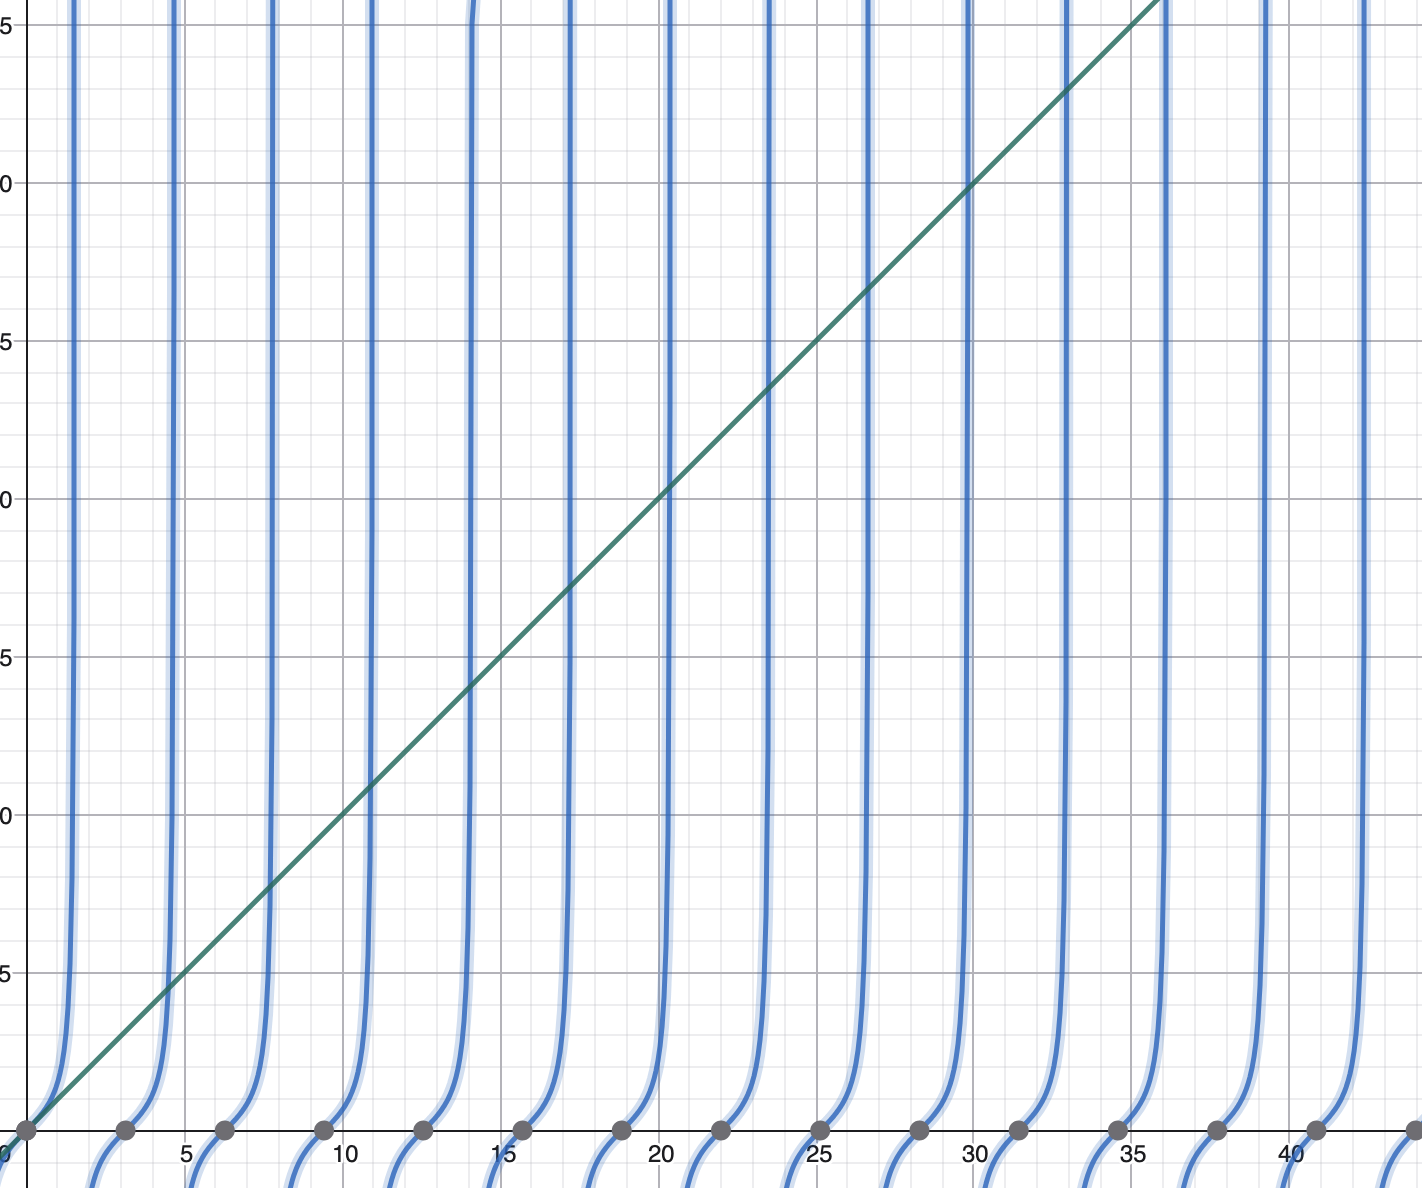
\includegraphics[width=0.8\textwidth,valign=t]{fig/prob4.10.png}
    
    For large $N,$ the solution is approximately located at 
    $(2N+\frac{1}{2})\pi.$

    $$
    ka = (2N+\frac{1}{2})\pi\Rightarrow
    \frac{\sqrt{2mE}}{\hbar}a=(2N+\frac{1}{2})\pi
    \Rightarrow 
    E = \frac{\hbar^2\pi^2}{2ma^2}(2N+\frac{1}{2})
    $$
    
\end{enumerate}

\subsection*{Sol. 11}
For $l=0,$ the differential equation is
$$
u'' = \frac{-2m(E-V)}{\hbar^2}u
$$

For $0<r<a,$
$$
u= A\sin k r,
$$
where $k=\frac{\sqrt{2m(E+V_0)}}{\hbar}.$
For $r>a,$
$$
u=Be^{-\frac{\sqrt{-2mE}}{\hbar}r}.
$$

The continuity condition requires 
$$
A\sin ka = Be^{-\frac{\sqrt{-2mE}}{\hbar}a}
$$
$$
kA\cos ka = -\frac{\sqrt{-2mE}}{\hbar}Be^{-\frac{\sqrt{-2mE}}{\hbar}a}
$$
Divide both equations give
$$
k\cot ka = -\frac{\sqrt{-2mE}}{\hbar}
\Rightarrow
\cot ka = -\sqrt{\frac{-E}{E+V_0}} 
=-\sqrt{\frac{V_0-\frac{k^2\hbar^2}{2m}}{\frac{k^2\hbar^2}{2m}}}
$$
$$
\cot z = -\sqrt{\frac{\frac{a^2V_02m}{\hbar^2}-z^2}{z^2}}
=-\sqrt{\frac{z_0^2}{z^2}-1},
$$
where $z = ka,$ $z_0 = \frac{a\sqrt{2mV_0}}{\hbar}.$ The ground state is thus the smallest positive $z$ that solves this transcendental equation.
 Note that the right hand side has zero at 
 $
 z=z_0,
 $
 so when $z_0<\frac{\pi}{2}\Rightarrow V_0<\frac{\pi^2\hbar^2}{8ma^2},$ there is no allowed bound state.

 \subsection*{Sol. 12}
 For $R_{30},$
 $$
 c_1 = \frac{2(0+0+1-3)}{(0+1)(0+2\cdot 0+2)}c_0
 =-2c_0
 $$
 $$
 c_2 = \frac{2(1+0+1-3)}{(1+1)(1+2\cdot 0+2)}c_1
 =\frac{-1}{3}c_1
 =\frac{2}{3}c_0
 $$
 $$
 c_3 = \frac{2(2+0+1-3)}{(2+1)(2+2\cdot 0+2)}c_2
 =0
 $$

 $$
 R_{30}(r)=
 \frac{1}{r}
 \frac{r}{3a} 
 e^{-\frac{r}{3a}}
 \left(\frac{2}{3}\left(\frac{r}{3a}\right)^2-2\frac{r}{3a}+1\right)c_0
 $$

 $$
 c_1 = \frac{2(0+1+1-3)}{(0+1)(0+2\cdot 1+2)}c_0
 =-\frac{1}{2}c_0
 $$
 $$
 c_2 = \frac{2(1+1+1-3)}{(1+1)(1+2\cdot 1+2)}c_1
 =0
 $$


 $$
 R_{31}(r)=
 \frac{1}{r}
 \left(\frac{r}{3a}\right)^2 
 e^{-\frac{r}{3a}}
 \left(-\frac{1}{2}\frac{r}{3a}+1\right)c_0
 $$

 $$
 c_1 = \frac{2(0+2+1-3)}{(0+1)(0+2\cdot 1+2)}c_0
 =0
 $$



 $$
 R_{32}(r)=
 \frac{1}{r}
 \left(\frac{r}{3a}\right)^3 
 e^{-\frac{r}{3a}}
 c_0
 $$

  \subsection*{Sol. 13}
  \begin{enumerate}
      \item 
      \begin{align*}
          \int_0^\infty 
          \frac{c_0^2}{4a^2}
          \left(
          1-\frac{r}{2a}
          \right)^2
          e^{-r/a}
          r^2dr=\frac{ac_0^2}{2}
          \Rightarrow c_0=\sqrt{\frac{2}{a}}
      \end{align*}
      \begin{align*}
          \psi_{200}(r,\theta,\phi)
          =
          \sqrt{\frac{2}{a}}
          \frac{1}{2a}
          \left(1-\frac{r}{2a}\right)
          e^{-r/2a}
          \sqrt{\frac{1}{4\pi}}
      \end{align*}

      \begin{align*}
          \int_0^\infty 
          \frac{c_0^2}{16a^4}
          r^2
          e^{-r/a}
          r^2dr=\frac{3ac_0^2}{2}
          \Rightarrow c_0=\sqrt{\frac{2}{3a}}
      \end{align*}
      \item 
      \begin{align*}
          \psi_{211}(r,\theta,\phi)
          =
          -\sqrt{\frac{2}{3a}}
          \frac{1}{4a^2}
          r
          e^{-r/2a}
          \sqrt{\frac{3}{8\pi}}
          \sin\theta e^{i\phi}
      \end{align*}
        \begin{align*}
          \psi_{210}(r,\theta,\phi)
          =
          \sqrt{\frac{2}{3a}}
          \frac{1}{4a^2}
          r
          e^{-r/2a}
          \sqrt{\frac{1}{4\pi}}
      \end{align*}
      \begin{align*}
          \psi_{21-1}(r,\theta,\phi)
          =\sqrt{\frac{2}{3a}}
          \frac{1}{4a^2}
          r
          e^{-r/2a}
          \sqrt{\frac{3}{8\pi}}
          \sin\theta 
          e^{-i\phi}
      \end{align*}
  \end{enumerate}

  \subsection*{Sol. 14}
  \begin{enumerate}
      \item 
      \begin{align*}
          L_0(x) = 1
      \end{align*}
      \begin{align*}
          L_1(x) = 
          \frac{e^x}{1}
          \frac{d}{dx}
          (e^{-x}x)
          =
          1-x
      \end{align*}
       \begin{align*}
          L_2(x) = 
          \frac{e^x}{2}
          \frac{d^2}{dx^2}
          (e^{-x}x^2)
          =
          \frac{1}{2}x^2
          -2x + 1
      \end{align*}
      \begin{align*}
          L_3(x) = 
          \frac{e^x}{6}
          \frac{d^3}{dx^3}
          (e^{-x}x^3)
          =
          -\frac{1}{6}
          x^3 
          +\frac{3}{2}x^2 
          -3x 
          + 1
      \end{align*}
      \item 
      $$
      v(\rho)
      =L^{2\cdot 2+1}_{5-2-1}
      (2\rho)
      =L^5_2(2\rho)
      $$
      $$
      L^5_2(x)
      =(-1)^5
      \frac{d^5}{dx^5}
      L_7(x)
      $$
      $$
      L_7(x)=
     \frac{e^x}{7!}
     \frac{d^7}{dx^7}
     (e^{-x}x^7)
     =
     -\frac{1}{7!}
     (x^7-49x^6+882x^5
     -7350x^4+29400x^3-52920x^2+35280x-5040)
      $$
      \begin{align*}
          L^5_2(x)
    =& \frac{1}{7!}
    (2520x^2-35280x+105840)\\
    =&
    \frac{1}{2}x^2-7x+21
      \end{align*}
      Therefore
      $$
      v(\rho)
      =2\rho^2-14\rho+21
      $$
      \item 
      $$
      c_1 = \frac{2(0+2+1-5)}{(0+1)(0+4+2)}c_0 = -\frac{2}{3}c_0
      $$
      $$
      c_2 = \frac{2(1+2+1-5)}
      {(1+1)(1+4+2)}c_1 = -\frac{1}{7}c_1=
      \frac{2}{21}c_0
      $$
      $$
      c_3 = \frac{2(2+2+1-5)}
      {(2+1)(2+4+2)}c_1 = 0
      $$
      Therefore 
      $$
      v(\rho)
      =(\frac{2}{21}\rho^2-\frac{2}{3}\rho+1)c_0
      $$
      
  \end{enumerate}

    \subsection*{Sol. 15}
    \begin{enumerate}
        \item 
        \begin{align*}
            \langle r\rangle
            =\int_0^\infty 
            \int_0^\pi 
            \int_0^{2\pi}
            r
            \frac{1}{\pi a^3}
            e^{-2r/a}
            r^2\sin\theta
            drd\theta d\phi
            =\frac{3a}{2}
        \end{align*}
        \begin{align*}
            \langle r^2\rangle
            =\int_0^\infty 
            \int_0^\pi 
            \int_0^{2\pi}
            r^2
            \frac{1}{\pi a^3}
            e^{-2r/a}
            r^2\sin\theta
            drd\theta d\phi
            =3a^2
        \end{align*}
        \item 
        $$
        \langle x\rangle = 0
        $$
        $$
        \langle x^2\rangle = a^2
        $$
        \item 
        $$
        \psi_{211}(r,\theta,\phi)
          =
          -\sqrt{\frac{2}{3a}}
          \frac{1}{4a^2}
          r
          e^{-r/2a}
          \sqrt{\frac{3}{8\pi}}
          \sin\theta e^{i\phi}
        $$

        \begin{align*}
            \langle x^2\rangle
            =&
            \int_0^\infty 
            \int_0^\pi 
            \int_0^{2\pi}
            r^2\sin^2\theta\cos^2\phi 
            \frac{2}{3a}
            \frac{1}{16a^4}
            r^2
            e^{-r/a}
            \frac{3}{8\pi}
            \sin^2(\theta )
            r^2\sin\theta 
            drd\theta d\phi\\
            =&12a^2
        \end{align*}
    \end{enumerate}

    \subsection*{Sol. 16}
    The probability density along the radial of the ground state is 
    $$
    \int_0^{2\pi}
    \int_0^{\pi}
    \frac{1}{\pi a^3}
            e^{-2r/a}
            r^2\sin\theta
            d\theta d\phi
            =
            \frac{4}{ a^3}
            e^{-2r/a}
            r^2,
    $$
    which attain the maximum at 
    $
    r=a.
    $

    \subsection*{Sol. 17}
    Note that $$
    [z,[H,z]] = 2zHz-z^2H-Hz^2.
    $$
    Also note that 
    \begin{align*}
    [H,z]=&\frac{1}{2m}([p^2_z, z])\\
    =&\frac{1}{2m}(p_z[p_z,z]+[p_z,z]p_z)\\
    =&\frac{-i\hbar p_z}{m}
    \end{align*}
    $$
    [z,[H,z]]
    =[z, \frac{-i\hbar p_z}{m}]
    =\frac{\hbar^2}{m}.
    $$
    Therefore
    $$
    \frac{\hbar^2}{m}
    =2\langle zHz\rangle
    -\langle z^2H\rangle
    -\langle Hz^2\rangle
    =2\langle zHz\rangle
    -2a^2E_1,
    $$
    $$
    \langle zHz\rangle
    =\frac{\hbar^2}{2m}+a^2E_1.
    $$


    \subsection*{Sol. 18}
    \begin{enumerate}
        \item 
        \begin{align*}
            \Psi(\bm{r},t)
            =&
            \frac{1}{\sqrt{2}}
            \left(
            \sqrt{\frac{2}{3a}}
            \frac{1}{4a^2}
            re^{-r/2a}
            \sqrt{\frac{3}{8\pi}}
            \sin\theta 
            (-e^{i\phi}+e^{-i\phi})
            \right)e^{-iE_2t/\hbar}\\
            =&
            \frac{-i}{2a^2}
            \sqrt{\frac{1}{8\pi a}}
            re^{-r/2a}
            \sin\theta 
            \sin\phi
            e^{-iE_2t/\hbar}
        \end{align*}
        \item 
        \begin{align*}
            \langle V\rangle
            =&
            -\frac{e^2}{4\pi\epsilon_0}
            \int_0^\infty 
            \int_0^\pi 
            \int_0^{2\pi}
            \frac{1}{r}
            \frac{1}{4a^4}
            \frac{1}{8\pi a}
            r^2e^{-r/a}
            \sin^2\theta 
            \sin^2\phi
            r^2\sin\theta drd\theta d\phi\\
            =&\frac{-e^2}{16\pi\epsilon_0a}\approx -6.8028eV
        \end{align*}
    \end{enumerate}

    \subsection*{Sol. 19}

    $$
    E_n(Z)
    =-\left[\frac{m_e}{2\hbar^2}
    \left(
    \frac{Ze^2}{4\pi\epsilon_0}
    \right)^2
    \right] 
    \frac{1}{n^2}
    $$

    $$
    E_1(Z)
    =-\left[\frac{m_e}{2\hbar^2}
    \left(
    \frac{Ze^2}{4\pi\epsilon_0}
    \right)^2
    \right] 
    $$

    $$
    a(Z)
    =\frac{4\pi\epsilon_0\hbar^2}{m_eZe^2}
    $$

    $$\mathcal{R}(Z)
    =\frac{m_e}{4\pi c\hbar^3}
    \left(
    \frac{Ze^2}{4\pi\epsilon_0}
    \right)^2
    $$


    \subsection*{Sol. 20}
    \begin{enumerate}
        \item 
        $$
        V(r)=\frac{-GMm_e}{r}
        $$
        \item By changing $\frac{e^2}{4\pi\epsilon_0}$ to $GMm_e,$
        $$
        a_g = \frac{\hbar^2}{GMm_e^2}
        $$
        The actual number
        is about $2.349
        \times 10^{-138}m.$
        \item 
        $$
        E_n = 
        -\left[
        \frac{m_e}{2\hbar^2}
        G^2M^2m_e^2
        \right]\frac{1}{n^2}
        $$
        $$
        -\left[
        \frac{m_e}{2\hbar^2}
        G^2M^2m_e^2
        \right]\frac{1}{n^2}
        =-\frac{GMm_e}{2r_0}
        \Rightarrow n = \sqrt{\frac{r_0}{a_g}}
        $$

        $r_0\approx 1.496\times10^{11}m,$
        so $n\approx 2.52\times10^{74}.$
        \item 
        From level $n$ to $n-1,$ the energy will release
        $$
        \frac{m_e}{2\hbar^2}G^2M^2m_e^2
        \frac{2n-1}{(n-1)^2n^2}
        \approx
        \frac{GMm_e}{a_gn^3}
        $$
        About $2.1\times10^{-41}J,$
        the corresponding wavelength is 
        $9.459\times 10^{15}m,$ just approximately a light year.
    \end{enumerate}

   \subsection*{Sol. 21}
   \begin{align*}
        \hbar^2 l(l+1)
       =&\langle f^{m}_l, L^2f^m_l\rangle\\
       =&
       \langle f^{m}_l, L_-L_+f^m_l\rangle
       +\langle f^{m}_l, L_z^2f^m_l\rangle
       +\hbar \langle f^{m}_l, L_zf^m_l\rangle\\
       =&(A^m_l)^2 + \hbar^2m^2 + \hbar^2 m\\
   \end{align*}
   $$
   A^m_l = \hbar\sqrt{l(l+1)-m(m+1)}
   =\hbar\sqrt{(l-m)(l+m+1)}
   $$
   \begin{align*}
        \hbar^2 l(l+1)
       =&\langle f^{m}_l, L^2f^m_l\rangle\\
       =&
       \langle f^{m}_l, L_+L_-f^m_l\rangle
       +\langle f^{m}_l, L_z^2f^m_l\rangle
       -\hbar \langle f^{m}_l, L_zf^m_l\rangle\\
       =&(B^m_l)^2 + \hbar^2m^2 - \hbar^2 m\\
   \end{align*}
   $$
   B^m_l = \hbar\sqrt{l(l+1)-m(m-1)}
   =\hbar\sqrt{(l+m)(l-m+1)}
   $$

   \subsection*{Sol. 22}
   \begin{enumerate}
       \item 
       $L_z=xp_y-yp_x,$
   so 
   $$
   [L_z, x]=i\hbar y,\;
   [L_z, y]=-i\hbar x,\;
   [L_z, z]=0\;
   $$
   $$
   [L_z, p_x]=i\hbar p_y,\;
   [L_z, p_y]=-i\hbar p_x,\;
   [L_z, p_z]=0\;
   $$
   \item 
   $$
   [L_z,L_x]
   =[L_z, yp_z-zp_y]
   =-i\hbar xp_z
   +i\hbar zp_x
   =i\hbar L_y
   $$
   \item 
   \begin{align*}
   [L_z, r^2]
   =&
   [L_z, x^2] + 
   [L_z, y^2] + 
   [L_z, z^2]\\
   =&x[L_z, x] + [L_z,x]x+
   y[L_z, y] + [L_z,y]y+
   z[L_z, z] + [L_z,z]z\\
   =&i\hbar xy+
   i\hbar yx
   -i\hbar yx 
   -i\hbar xy  = 0
   \end{align*}
   \begin{align*}
   [L_z, p^2]
   =&
   [L_z, p_x^2] + 
   [L_z, p_y^2] + 
   [L_z, p_z^2]\\
   =&p_x[L_z, p_x] + [L_z,p_x]p_x+
   p_y[L_z, p_y] + [L_z,p_y]p_y+
   p_z[L_z, p_z] + [L_z,p_z]p_z\\
   =&i\hbar p_xp_y+
   i\hbar p_yp_x
   -i\hbar p_yp_x 
   -i\hbar p_xp_y  = 0
   \end{align*}
   \item 
   \begin{align*}
       [L_z, r] =& [xp_y - yp_x, r]\\
       =&x[p_y,r]-y[p_x,r]\\
       =&-i\hbar x\frac{y}{r} +i\hbar \frac{x}{r} = 0.
   \end{align*}
   Expand $V$ in Taylor series, we then obtain that $L_z$ commutes with $H,$ and therefore all three components of the angular momentum commute with $H.$
   
   \end{enumerate}


   \subsection*{Sol. 23}
   \begin{enumerate}
       \item 
       Note that 
   \begin{align*}
   [V, L_x] = &
   [V, yp_z-zp_y]\\
   =&[V, yp_z] - [V,zp_y]\\
   =&y[V,p_z] + [V,y]p_z - z[V,p_y]-[V,z]p_y\\
   =&i\hbar yV_z- i\hbar zV_y,
   \end{align*}
   similarly 
   $$
   [V, L_y]=i\hbar(zV_y-yV_z),
   $$
   $$
   [V, L_z]=i\hbar(xV_y-yV_x).
   $$
   \begin{align*}
       \frac{d}{dt}\langle \bm{L}\rangle
       =&\frac{i}{\hbar}
       \langle [H, \bm{L}]\rangle\\
       =&\frac{i}{\hbar}\langle[V, (L_x, L_y, L_z)]\rangle\\
       =&-\langle(yV_z-zV_y, -xV_z+zV_x, xV_y-yV_x)\rangle
   \end{align*}
   \begin{align*}
       \bm{r}\times (-\nabla V)
       =-(yV_z-zV_y, -xV_z+zV_x, xV_y-yV_x).
   \end{align*}
   Hence 
   $$
   \frac{d}{dt}\langle\bm{L}\rangle
   =\langle \bm{N}\rangle.
   $$
   \item 
   In spherical coordinate, $$\nabla V=V_r\hat{r},$$ so the cross product with $\bm{r}=r\hat{r}$ cancels.
   \end{enumerate}

   \subsection*{Sol. 24}
\begin{enumerate}
    \item 
    \begin{align*}
        L_+L_-f
        =&-\hbar 
        e^{i\phi}
        \left(
        \frac{\partial}{\partial\theta}
        +i\cot\theta  
        \frac{\partial}{\partial\phi}
        \right)
        \hbar 
        e^{-i\phi}
        \left(
        \frac{\partial}{\partial\theta}
        -
        i\cot\theta  
        \frac{\partial}{\partial\phi}
        \right)f\\
        =&-\hbar^2 
        e^{i\phi}
        \left(
        \frac{\partial}{\partial\theta}
        +i\cot\theta  
        \frac{\partial}{\partial\phi}
        \right)
        e^{-i\phi}
        (f_\theta
        -i\cot\theta f_\phi)\\
        =&
        -\hbar^2
        e^{i\phi}
        (e^{-i\phi}f_{\theta\theta} 
        -ie^{-i\phi}(-\csc^2\theta f_\phi + \cot\theta f_{\phi\theta})\\
        &+i\cot\theta
        (-ie^{-i\phi}f_\theta + 
        e^{-i\phi}f_{\theta\phi})
        +\cot^2\theta(-ie^{-i\phi}f_\phi + e^{-i\phi}f_{\phi\phi})
        )\\
        =&-\hbar^2(
        f_{\theta\theta}
        +
        if_\phi 
        +\cot\theta f_{\theta}
        +\cot^2\theta f_{\phi\phi}
        ).
    \end{align*}    
    $$
    L_+L_- = 
    -\hbar^2
    \left(
    \frac{\partial^2}{\partial\theta^2 }
    +\cot\theta
    \frac{\partial}{\partial\theta}
    +\cot^2\theta
    \frac{\partial^2}{\partial\phi^2}
    +i\frac{\partial}{\partial\phi}
    \right)
    $$
    \item 
    \begin{align*}
        L^2=&L_+L_-+L_z^2 -\hbar L_z\\
        =&
        -\hbar^2
    \left(
    \frac{\partial^2}{\partial\theta^2 }
    +\cot\theta
    \frac{\partial}{\partial\theta}
    +\cot^2\theta
    \frac{\partial^2}{\partial\phi^2}
    +i\frac{\partial}{\partial\phi}
    \right)
    -\hbar^2\frac{\partial^2}{\partial\phi^2}
    +i\hbar^2\frac{\partial}{\partial\phi}\\
    =&-\hbar^2\left(
    \frac{\partial^2}{\partial\theta^2 }
    +\cot\theta
    \frac{\partial}{\partial\theta}
    -\csc^2\theta
    \frac{\partial^2}{\partial\phi^2}
    \right)
    \end{align*}
    
\end{enumerate}

   \subsection*{Sol. 25}
   \begin{enumerate}
       \item $$
       L_+Y^l_l = 0
       $$
       \item 
       $$
       \hbar e^{i\phi}
       (\frac{\partial}{\partial\theta}+i\cot\theta\frac{\partial}{\partial\phi})Y^l_l = 0
       $$
       Also, 
       $$
       -i\hbar\frac{\partial}{\partial\phi} Y^l_l = \hbar lY^l_l
       \Rightarrow 
       Y^l_l = A(\theta)e^{il\phi}.
       $$
       $$
       \frac{\partial}{\partial\theta}
       Y^l_l 
       -\cot\theta lY^l_l = 0
       $$
       $$
       A(\theta)= C\sin^l\theta,
       $$
       so 
       $$
       Y^l_l = C\sin^l\theta e^{il\phi}.
       $$
       \item 
       Let $I_{2l+1} = \int_0^{\pi}\sin^{2l+1}\theta d\theta,$
       then 
       \begin{align*}
           I_{2l+1} =&  \int_0^{\pi}\sin^{2l+1}\theta d\theta\\
           =&-\sin^{2l}\theta \cos\theta 
           \bigg|_0^\pi 
           +2l\int\sin^{2l-1}\theta \cos^2\theta d\theta \\
           =&2l(I_{2l-1} - I_{2l+1})
       \end{align*}
       \begin{align*}
      I_{2l+1} =& \frac{2l}{2l+1}I_{2l-1}\\
      =&\frac{2l}{2l+1}\frac{2l-2}{2l-1}I_{2l-3}\\
      =&\frac{2l}{2l+1}\frac{2l-2}{2l-1}\dots \frac{2}{3}I_1\\
      =&\frac{2^{2l}(l!)^22}{(2l+1)!}
       \end{align*}

       \begin{align*}
           \int_0^{2\pi}
           \int_0^\pi
           C^2\sin^{2l}\theta 
           \sin\theta d\theta d\phi
           =&C^22\pi\frac{2^{2l}(l!)^22}{(2l+1)!}
           \Rightarrow 
           C = (-1)^l\sqrt{\frac{(2l+1)!}{\pi}}
           \frac{1}{2^{l+1}l!}
       \end{align*}
      
   \end{enumerate}
   \subsection*{Sol. 26}
   \begin{align*}
       L_+Y^{1}_2 =& -\sqrt{\frac{15}{8\pi}}
       \hbar e^{i\phi}
       \left(\frac{\partial}{\partial\theta}
       +i\cot\theta 
       \frac{\partial}{\partial\phi}\right)
       \sin\theta \cos\theta e^{i\phi}\\
       =&
       -\sqrt{\frac{15}{8\pi}}
       \hbar e^{i\phi}
       [(\cos^2\theta -\sin^2\theta)e^{i\phi}
       +i\cot\theta 
       \sin\theta \cos\theta ie^{i\phi}
       ]\\
       =&
       \sqrt{\frac{15}{8\pi}}
       \hbar e^{2i\phi}
       \sin^2\theta 
   \end{align*}
   By 4.121, 
   $$
   A^1_2 = 
   2\hbar,
   $$
   so 
   $$
    Y^2_2
    =\sqrt{\frac{15}{32\pi}}
    e^{2i\phi}
    \sin^2\theta.
   $$

   \subsection*{Sol. 27}
   \begin{enumerate}
       \item 
       Let $\omega$ be the angular speed, 
       $r_1=\frac{m_2a}{m_1+m_2},$ 
       $p_1 = \frac{m_1m_2a}{m_1+m_2}\omega,$
       $r_2=\frac{m_1a}{m_1+m_2},$ 
       $p_2 = \frac{m_1m_2a}{m_1+m_2}\omega$
       \begin{align*}
           L = &
       \frac{m_2a}{m_1+m_2}
       \frac{m_1m_2a}{m_1+m_2}\omega+
       \frac{m_1a}{m_1+m_2}\frac{m_1m_2a}{m_1+m_2}\omega\\
       =&\frac{m_1m_2a^2}{m_1+m_2}\omega = I\omega,
       \end{align*}
       where $I=\frac{m_1m_2}{m_1+m_2}a^2.$

       The energy is 
       \begin{align*}
           E =& \frac{p_1^2}{2m_1}
           +\frac{p_2^2}{2m_2}\\
           =&
           \left(\frac{m_1m_2a}{m_1+m_2}\omega\right)^2
           \frac{m_1+m_2}{2m_1m_2}\\
           =&\frac{1}{2}I\omega^2      \\
           =&\frac{L^2}{2I}.
       \end{align*}
       By the theory developed above, the allowed eigenvalues of $L^2$ are $\hbar n(n+1),$ for $n=0,1,\dots.$ Therefore, the allowed energies of this rigid rotor are $$
       E_n = \frac{\hbar^2}{2I}n(n+1).
       $$
       \item The Hamiltonian is $\frac{L^2}{2I},$ so the normalized eigenfunctions are the spherical harmonics. For the energy level $n,$ there are $2n+1$ possible $m$ values.
       \item 
       The difference between two adjacent energy level is 
       $$
       E_{n+1}
       -E_n
       =\frac{\hbar^2}{I}
       (n+1).
       $$
       Any energy differences is therefore 
       $\frac{\hbar^2j}{I},$ for $j=1,2,3\dots.$
       $$
       \nu_j=\frac{\hbar^2j}{I}\frac{1}{2\pi\hbar}
       =\frac{\hbar j}{2\pi I}.
       $$
       \item 
       The frequency separation is $\frac{\hbar}{2\pi I}.$
       From the figure, the frequency separation is approximately 
       $1.2\times10^{11}Hz.$
       $$
       a = \sqrt{\frac{\hbar}{2\pi\Delta\nu}\frac{m_1+m_2}{m_1m_2}}\approx 1.108\times 10^{-10}m.
       $$
   \end{enumerate}
   \subsection*{Sol. 28}
   Assume the angular speed is $\omega.$
   \begin{align*}
       \frac{1}{2}\hbar = 
       &\int_0^{2\pi}\int_{0}^\pi\int_0^{r_c} 
       r^2\sin^2\theta\omega
       \rho
       r^2\sin\theta drd\theta d\phi\\
       =&\frac{8\pi r_c^5}{15}\omega 
       \frac{m}{\frac{4}{3}\pi r_c^3}\\
       =&\frac{2r_c^2\omega m}{5}
   \end{align*}
   The point at the equator moves at speed
   $$
   v = r_c\omega = 
   \frac{\hbar}{2}
   \frac{5}{2r_c m}
   =\frac{5\hbar\pi\epsilon_0c^2}{e^2}\approx 5.14\times 10^{10}m/s.
   $$
   \subsection*{Sol. 29}
\begin{enumerate}
    \item 
    \begin{align*}
        S_xS_y 
        -S_yS_x
    =&
    \frac{\hbar^2}{4}
    \begin{pmatrix}
    0 & 1 \\
    1 & 0
    \end{pmatrix}
    \begin{pmatrix}
    0 & -i \\
    i & 0
    \end{pmatrix}
    -
    \frac{\hbar^2}{4}
    \begin{pmatrix}
    0 & -i \\
    i & 0
    \end{pmatrix}
    \begin{pmatrix}
    0 & 1 \\
    1 & 0
    \end{pmatrix}\\
    =&
    \frac{\hbar^2}{4}
    \begin{pmatrix}
        i & 0\\
        0 & -i
    \end{pmatrix}
    -
    \frac{\hbar^2}{4}
    \begin{pmatrix}
        -i & 0\\
        0 & i
    \end{pmatrix}
    \\
    =&
    \frac{\hbar^2}{4}
    \begin{pmatrix}
        2i & 0\\
        0 & -2i
    \end{pmatrix}\\
    =&i\hbar S_z
    \end{align*}

    \begin{align*}
        S_yS_z 
        -S_zS_y
    =&
    \frac{\hbar^2}{4}
    \begin{pmatrix}
    0 & -i \\
    i & 0
    \end{pmatrix}
    \begin{pmatrix}
    1 & 0 \\
    0 & -1
    \end{pmatrix}
    -
    \frac{\hbar^2}{4}
    \begin{pmatrix}
    1 & 0 \\
    0 & -1
    \end{pmatrix}
    \begin{pmatrix}
    0 & -i \\
    i & 0
    \end{pmatrix}\\
    =&
    \frac{\hbar^2}{4}
    \begin{pmatrix}
        0 & i\\
        i & 0
    \end{pmatrix}
    -
    \frac{\hbar^2}{4}
    \begin{pmatrix}
        0 & -i\\
        -i & 0
    \end{pmatrix}
    \\
    =&
    \frac{\hbar^2}{4}
    \begin{pmatrix}
        0 & 2i\\
        2i & 0
    \end{pmatrix}\\
    =&i\hbar S_x
    \end{align*}

    \begin{align*}
        S_zS_x
        -S_xS_z
    =&
    \frac{\hbar^2}{4}
    \begin{pmatrix}
    1 & 0 \\
    0 & -1
    \end{pmatrix}
    \begin{pmatrix}
    0 & 1 \\
    1 & 0
    \end{pmatrix}
    -
    \frac{\hbar^2}{4}
    \begin{pmatrix}
    0 & 1 \\
    1 & 0
    \end{pmatrix}
    \begin{pmatrix}
    1 & 0 \\
    0 & -1
    \end{pmatrix}\\
    =&
    \frac{\hbar^2}{4}
    \begin{pmatrix}
        0 & 1\\
        -1 & 0
    \end{pmatrix}
    -
    \frac{\hbar^2}{4}
    \begin{pmatrix}
        0 & -1\\
        1 & 0
    \end{pmatrix}
    \\
    =&
    \frac{\hbar^2}{4}
    \begin{pmatrix}
        0 & 2\\
        -2 & 0
    \end{pmatrix}\\
    =&i\hbar S_y
    \end{align*}
    \item 
    $$
    \sigma_x\sigma_x = 
    \begin{pmatrix}
        0 & 1\\
        1 & 0
    \end{pmatrix}
    \begin{pmatrix}
        0 & 1\\
        1 & 0
    \end{pmatrix}
    =\begin{pmatrix}
        1 & 0\\
        0 & 1
    \end{pmatrix}
    =I
    $$
    
    $$
    \sigma_x\sigma_y = 
    \begin{pmatrix}
        0 & 1\\
        1 & 0
    \end{pmatrix}
    \begin{pmatrix}
        0 & -i\\
        i & 0
    \end{pmatrix}
    =\begin{pmatrix}
        i & 0\\
        0 & -i
    \end{pmatrix}
    =i\sigma_z
    $$

    $$
    \sigma_x\sigma_z = 
    \begin{pmatrix}
        0 & 1\\
        1 & 0
    \end{pmatrix}
    \begin{pmatrix}
        1 & 0\\
        0 & -1
    \end{pmatrix}
    =\begin{pmatrix}
        0 & -1\\
        1 & 0
    \end{pmatrix}
    =-i\sigma_y
    $$



    $$
    \sigma_y\sigma_x = 
    \begin{pmatrix}
        0 & -i\\
        i & 0
    \end{pmatrix}
    \begin{pmatrix}
        0 & 1\\
        1 & 0
    \end{pmatrix}
    =\begin{pmatrix}
        -i & 0\\
        0 & i
    \end{pmatrix}
    =-i\sigma_z
    $$
    
    $$
    \sigma_y\sigma_y = 
    \begin{pmatrix}
        0 & -i\\
        i & 0
    \end{pmatrix}
    \begin{pmatrix}
        0 & -i\\
        i & 0
    \end{pmatrix}
    =\begin{pmatrix}
        1 & 0\\
        0 & 1
    \end{pmatrix}
    =I
    $$

    $$
    \sigma_y\sigma_z = 
    \begin{pmatrix}
        0 & -i\\
        i & 0
    \end{pmatrix}
    \begin{pmatrix}
        1 & 0\\
        0 & -1
    \end{pmatrix}
    =\begin{pmatrix}
        0 & i\\
        i & 0
    \end{pmatrix}
    =i\sigma_x
    $$
    %%%%

    $$
    \sigma_z\sigma_x = 
    \begin{pmatrix}
        1 & 0\\
        0 & -1
    \end{pmatrix}
    \begin{pmatrix}
        0 & 1\\
        1 & 0
    \end{pmatrix}
    =\begin{pmatrix}
        0 & 1\\
        -1 & 0
    \end{pmatrix}
    =i\sigma_y
    $$
    
    $$
    \sigma_z\sigma_y = 
    \begin{pmatrix}
        1 & 0\\
        0 & -1
    \end{pmatrix}
    \begin{pmatrix}
        0 & -i\\
        i & 0
    \end{pmatrix}
    =\begin{pmatrix}
        0 & -i\\
        -i & 0
    \end{pmatrix}
    =-i\sigma_x
    $$

    $$
    \sigma_z\sigma_z = 
    \begin{pmatrix}
        1 & 0\\
        0 & -1
    \end{pmatrix}
    \begin{pmatrix}
        1 & 0\\
        0 & -1
    \end{pmatrix}
    =I
    $$
    
\end{enumerate}

   \subsection*{Sol. 30}
   \begin{enumerate}
       \item $\frac{1}{5}$
       \item 
       \begin{align*}
           \langle S_x\rangle
           =&\frac{1}{25}
           \frac{\hbar}{2}
           \begin{pmatrix}
               -3i & 4
           \end{pmatrix}
           \begin{pmatrix}
               0 & 1 \\
               1 & 0
           \end{pmatrix}
           \begin{pmatrix}
               3i\\4
           \end{pmatrix}\\
           =& \frac{\hbar}{50}
           \begin{pmatrix}
               -3i & 4
           \end{pmatrix}
           \begin{pmatrix}
               4 \\ 3i
           \end{pmatrix}\\
           =&0
       \end{align*}
       \begin{align*}
           \langle S_y\rangle
           =&\frac{1}{25}
           \frac{\hbar}{2}
           \begin{pmatrix}
               -3i & 4
           \end{pmatrix}
           \begin{pmatrix}
               0 & -i \\
               i & 0
           \end{pmatrix}
           \begin{pmatrix}
               3i\\4
           \end{pmatrix}\\
           =& \frac{\hbar}{50}
           \begin{pmatrix}
               -3i & 4
           \end{pmatrix}
           \begin{pmatrix}
               -4i \\ -3
           \end{pmatrix}\\
           =&\frac{-12\hbar}{25}
       \end{align*}
       \begin{align*}
           \langle S_z\rangle
           =&\frac{1}{25}
           \frac{\hbar}{2}
           \begin{pmatrix}
               -3i & 4
           \end{pmatrix}
           \begin{pmatrix}
               1 & 0 \\
               0 & -1
           \end{pmatrix}
           \begin{pmatrix}
               3i\\4
           \end{pmatrix}\\
           =& \frac{\hbar}{50}
           \begin{pmatrix}
               -3i & 4
           \end{pmatrix}
           \begin{pmatrix}
               3i \\ -4
           \end{pmatrix}\\
           =&\frac{-7\hbar}{50}
       \end{align*}
       \item 

        \begin{align*}
           \langle S^2_x\rangle
           =
           \langle S^2_y\rangle
           =
           \langle S^2_z\rangle
           =
           \frac{\hbar^2}{4}
       \end{align*}

       $$
       \sigma_{S_x}
       =\frac{\hbar}{2},\;
       \sigma_{S_y}
       =\frac{7\hbar}{50},\;
       \sigma_{S_z}
       =\frac{12\hbar}{25}
       $$
       \item 
       $$
       \sigma_{S_x}\sigma_{S_y}
       =\frac{7\hbar^2}{100}\geq 
       \frac{\hbar}{2}\frac{7\hbar}{50}=|\langle S_z\rangle|
       $$
       $$
       \sigma_{S_x}\sigma_{S_z}
       =\frac{6\hbar^2}{25}\geq 
       \frac{\hbar}{2}\frac{12\hbar}{25}=|\langle S_y\rangle|
       $$
       $$
       \sigma_{S_y}\sigma_{S_z}
       =\frac{42\hbar^2}{625}\geq 
       0=|\langle S_x\rangle|
       $$
   \end{enumerate}

   \subsection*{Sol. 31}
   \begin{align*}
       \langle S_x\rangle =& 
       \frac{\hbar}{2}
       \begin{pmatrix}
           \bar a & \bar b
       \end{pmatrix}
       \begin{pmatrix}
           0 & 1 \\
           1 & 0
       \end{pmatrix}
       \begin{pmatrix}
           a \\ b 
       \end{pmatrix}\\
       =&
       \frac{\hbar}{2}
        \begin{pmatrix}
           \bar a & \bar b
       \end{pmatrix}
       \begin{pmatrix}
           b \\ a 
       \end{pmatrix}\\
       =&\frac{\hbar}{2}(\bar a b + \bar b a)
\end{align*}
        \begin{align*}
       \langle S_y\rangle =& 
       \frac{\hbar}{2}
       \begin{pmatrix}
           \bar a & \bar b
       \end{pmatrix}
       \begin{pmatrix}
           0 & -i \\
           i & 0
       \end{pmatrix}
       \begin{pmatrix}
           a \\ b 
       \end{pmatrix}\\
       =&
       \frac{\hbar}{2}
        \begin{pmatrix}
           \bar a & \bar b
       \end{pmatrix}
       \begin{pmatrix}
           -bi \\ ai 
       \end{pmatrix}\\
       =&\frac{\hbar}{2}(-i\bar a b + i\bar b a)
   \end{align*}
   \begin{align*}
       \langle S_z\rangle =& 
       \frac{\hbar}{2}
       \begin{pmatrix}
           \bar a & \bar b
       \end{pmatrix}
       \begin{pmatrix}
           1 & 0 \\
           0 & -1
       \end{pmatrix}
       \begin{pmatrix}
           a \\ b 
       \end{pmatrix}\\
       =&
       \frac{\hbar}{2}
        \begin{pmatrix}
           \bar a & \bar b
       \end{pmatrix}
       \begin{pmatrix}
           a \\ -b 
       \end{pmatrix}\\
       =&\frac{\hbar}{2}(a\bar a  - b\bar b )\\
       =& \frac{\hbar}{2} (|a|^2-|b|^2)
   \end{align*}

   \begin{align*}
       \langle S^2_x\rangle=
       \langle S^2_y\rangle=
       \langle S^2_z\rangle=
       \frac{\hbar^2}{4}
   \end{align*}
   $$
   \langle S^2_x\rangle + \langle S^2_y\rangle +\langle S^2_z\rangle
   =\frac{3}{4}\hbar^2
   $$

   \subsection*{Sol. 32}
   \begin{enumerate}
       \item 
       $$
       \begin{vmatrix}
       -t & -i\frac{\hbar}{2}\\
       i\frac{\hbar}{2} & -t
       \end{vmatrix}
       =
       t^2-\frac{\hbar^2}{4}
       $$

       $$
       \chi_+^{(y)}
       =
       \frac{1}{\sqrt{2}}
       \begin{pmatrix}
           -i\\1
       \end{pmatrix}
       ,\;
       \text{eigenvalue }
       +\frac{\hbar}{2}
       $$

       $$
       \chi_-^{(y)}
       =
       \frac{1}{\sqrt{2}}
       \begin{pmatrix}
           i\\1
       \end{pmatrix}
       ,\;
       \text{eigenvalue }
       -\frac{\hbar}{2}
       $$
    \item 
    $$
    \begin{pmatrix}
        a\\b
    \end{pmatrix}
    =
    \frac{1}{\sqrt{2}}
    (ia + b)
    \chi_+^{(y)}
    +\frac{1}{\sqrt{2}}
    (-ia+b)
    \chi_-^{(y)}
    $$
    We might get 
    $\frac{\hbar}{2}$ with probability 
    $\frac{|ia+b|^2}{2},$ 
    $\frac{-\hbar}{2}$ with probability 
    $\frac{|-ia+b|^2}{2}.$

    $$
    \frac{|-ia+b|^2}{2} + 
    \frac{|ia+b|^2}{2}
    =\frac{1}{2}
    (|a|^2 + ia\bar b -ib\bar a + |b|^2 
    |a|^2 - ia\bar b + ib\bar a + |b|^2 )
    =|a|^2 + |b|^2 = 1
    $$
    \item $\frac{\hbar^2}{4}$ with probability 1.
   \end{enumerate}

   \subsection*{Sol. 33}
   \begin{align*}
       S_r = &
       \sin\theta \cos\phi S_x + 
       \sin\theta \sin\phi S_y + 
       \cos\theta S_z\\
       =&
       \frac{\hbar}{2}
       \begin{pmatrix}
           0 & \sin\theta \cos\phi\\
           \sin\theta \cos\phi & 0
       \end{pmatrix}
       +
       \frac{\hbar}{2}
       \begin{pmatrix}
           0 & -i\sin\theta \sin\phi\\
           i\sin\theta \sin\phi & 0
       \end{pmatrix}
       +\frac{\hbar}{2}
       \begin{pmatrix}
           \cos\theta & 0\\
           0 & - \cos\theta
       \end{pmatrix}\\
       =&\frac{\hbar}{2}
       \begin{pmatrix}
       \cos\theta & \sin\theta e^{-i\phi} \\
       \sin\theta e^{i\phi} & -\cos\theta
       \end{pmatrix}
   \end{align*}

   \begin{align*}
       \begin{vmatrix}
       \frac{\hbar}{2}\cos\theta - t & \frac{\hbar}{2}\sin\theta e^{-i\phi} \\
       \frac{\hbar}{2}\sin\theta e^{i\phi} & -\frac{\hbar}{2}\cos\theta - t
       \end{vmatrix}
       =t^2-\frac{\hbar^2}{4}
   \end{align*}

   $$
       \chi_+^{(r)}
       =
       \begin{pmatrix}
           \cos\frac{\theta}{2}\\
           e^{i\phi}\sin\frac{\theta}{2}
       \end{pmatrix}
       ,\;
       \text{eigenvalue }
       +\frac{\hbar}{2}
       $$

       $$
       \chi_-^{(r)}
       =
       \begin{pmatrix}
           e^{-i\phi}
           \sin\frac{\theta}{2}
           \\
           -\cos\frac{\theta}{2}
       \end{pmatrix}
       ,\;
       \text{eigenvalue }
       -\frac{\hbar}{2}
       $$

       \subsection*{Sol. 34}
       There are three eigensates of $S_z.$
       $$
       S_z =
       \hbar
       \begin{pmatrix}
           1 & 0 & 0\\
           0 & 0 & 0\\
           0 & 0 & -1
       \end{pmatrix}
       $$

       $$
       S_+ =
       \hbar
       \begin{pmatrix}
           0 & \sqrt{2} & 0\\
           0 & 0 & \sqrt{2}\\
           0 & 0 & 0
       \end{pmatrix}
       $$

       $$
       S_- =
       \hbar
       \begin{pmatrix}
           0 & 0 & 0\\
           \sqrt{2} & 0 & 0\\
           0 & \sqrt{2} & 0
       \end{pmatrix}
       $$

       $$
       S_x = 
       \hbar 
       \begin{pmatrix}
           0 & \frac{\sqrt{2}}{2} & 0\\
           \frac{\sqrt{2}}{2} & 0 & \frac{\sqrt{2}}{2}\\
           0 & \frac{\sqrt{2}}{2} & 0
       \end{pmatrix}
       $$

       $$
       S_y = 
       \hbar 
       \begin{pmatrix}
           0 & \frac{\sqrt{2}}{2i} & 0\\
           \frac{-\sqrt{2}}{2i} & 0 & \frac{\sqrt{2}}{2i}\\
           0 & \frac{-\sqrt{2}}{2i} & 0
       \end{pmatrix}
       $$

       \subsection*{Sol. 35}
       \begin{enumerate}
           \item 
           $$
           \langle S_x\rangle
           =\frac{\hbar}{2}
           \sin\alpha
           \cos(\gamma B_0t)
           $$
           The probability of getting 
           $\frac{\hbar}{2}$ is 
           $$
           \frac{1}{2}
           (
           1 + \sin\alpha\cos(\gamma B_0t)
           ).
           $$
           \item 
           $$
           \langle S_y\rangle
           =-\frac{\hbar}{2}
           \sin\alpha
           \sin(\gamma B_0t)
           $$
           The probability of getting 
           $\frac{\hbar}{2}$ is 
           $$
           \frac{1}{2}
           (
           1 - \sin\alpha\sin(\gamma B_0t)
           ).
           $$
           \item 
           $$
           \langle S_z\rangle
           =\frac{\hbar}{2}
           \cos\alpha
           $$
           The probability of getting 
           $\frac{\hbar}{2}$ is 
           $$
           \frac{1}{2}
           (
           1 + \cos\alpha
           )=\cos^2\left(\frac{\alpha}{2}\right).
           $$
       \end{enumerate}

       \subsection*{Sol. 36}
       \begin{enumerate}
           \item $$
           H = -\gamma B_0\cos(\omega t)S_z
           =-\frac{\gamma B_0\hbar}{2}
           \cos(\omega t)
           \begin{pmatrix}
               1 & 0 \\
               0 & -1
           \end{pmatrix}
           $$
           \item 
           \begin{align*}
               i\hbar \chi' = 
               -\frac{\gamma B_0\hbar}{2}
           \cos(\omega t)
           \begin{pmatrix}
               1 & 0 \\
               0 & -1
           \end{pmatrix}
           \chi
           \end{align*}
           $$
           \chi_1'=
           \frac{i\gamma B_0}{2}
           \cos(\omega t)\chi_1
           \Rightarrow
           \chi_1 = A_1\exp(\frac{i\gamma B_0}{2\omega}\sin(\omega t))
           $$
           $$
           \chi_2'=
           \frac{-i\gamma B_0}{2}
           \cos(\omega t)\chi_2
           \Rightarrow
           \chi_2 = A_2\exp(\frac{-i\gamma B_0}{2\omega}\sin(\omega t))
           $$

           $\chi_+^{(x)}=
           \frac{1}{\sqrt{2}}
           \begin{pmatrix}
               1\\1
           \end{pmatrix},$
           so
           $$
           \chi =
           \frac{1}{\sqrt{2}}
            \begin{pmatrix}
                \exp(\frac{i\gamma B_0}{2\omega}\sin(\omega t)) \\
                \exp(\frac{-i\gamma B_0}{2\omega}\sin(\omega t))
            \end{pmatrix}
           $$
           \item 
           $$
           \langle \chi_+^{(x)}, \chi\rangle
           =\frac{1}{2}(\exp(\frac{i\gamma B_0}{2\omega}\sin(\omega t)) + 
           \exp(\frac{-i\gamma B_0}{2\omega}\sin(\omega t)))
           =\cos\left(\frac{\gamma B_0}{2\omega}\sin(\omega t))\right),
           $$
           so the probability of measuring $-\frac{\hbar}{2}$ is 
           $$
           1-\cos^2\left(\frac{\gamma B_0}{2\omega}\sin(\omega t)\right)
           =\sin^2\left(\frac{\gamma B_0}{2\omega}\sin(\omega t)\right).
           $$
           \item 
            $$
            \frac{\gamma B_0}{2\omega}\geq \frac{\pi}{2}
            \Rightarrow B_0\geq \frac{\pi\omega}{\gamma}.
            $$  
       \end{enumerate}

       \subsection*{Sol. 37}
       \begin{enumerate}
           \item \begin{align*}
               S_-|10\rangle =& 
               (S_-^{(1)} + S_-^{(2)})
           (\frac{1}{\sqrt{2}}
           |\updownarrows\rangle
           +\frac{1}{\sqrt{2}}
           |\downuparrows\rangle)\\
           =&
           \frac{\hbar}{\sqrt{2}}
           |\downdownarrows\rangle
           +
           \frac{\hbar}{\sqrt{2}}
           |\downdownarrows\rangle
           \\
           =&\sqrt{2}\hbar|1-1\rangle
           \end{align*}
           \item 
           \begin{align*}
               S_+|00\rangle =& 
               (S_+^{(1)} + S_+^{(2)})
           (\frac{1}{\sqrt{2}}
           |\updownarrows\rangle
           -\frac{1}{\sqrt{2}}
           |\downuparrows\rangle)\\
           =&
           \frac{-\hbar}{\sqrt{2}}
           |\upuparrows\rangle
           +
           \frac{\hbar}{\sqrt{2}}
           |\upuparrows\rangle
           \\
           =&0
           \end{align*}
           \begin{align*}
               S_-|00\rangle =& 
               (S_-^{(1)} + S_-^{(2)})
           (\frac{1}{\sqrt{2}}
           |\updownarrows\rangle
           -\frac{1}{\sqrt{2}}
           |\downuparrows\rangle)\\
           =&
           \frac{\hbar}{\sqrt{2}}
           |\downdownarrows\rangle
           -
           \frac{\hbar}{\sqrt{2}}
           |\downdownarrows\rangle
           \\
           =&0
           \end{align*}
           \item 
           \begin{align*}
               S^2|11\rangle = 
               &
               ((S^{(1)})^2 +(S^{(2)})^2
               +2\bm{S}^{(1)}
               \cdot
               \bm{S}^{(2)})
               |\upuparrows\rangle
           \end{align*}
           \begin{align*}
               \bm{S}^{(1)}
               \cdot
               \bm{S}^{(2)}
               |\upuparrows\rangle
               =&
               (S_x^{(1)}|\uparrow\rangle)
               (S_x^{(2)}|\uparrow\rangle)+
               (S_y^{(1)}|\uparrow\rangle)
               (S_y^{(2)}|\uparrow\rangle)+
               (S_z^{(1)}|\uparrow\rangle)
               (S_z^{(2)}|\uparrow\rangle)\\
               =&
               (\frac{\hbar}{2}|\downarrow\rangle)
               (\frac{\hbar}{2}|\downarrow\rangle)
               +
               (-i\frac{\hbar}{2}|\downarrow\rangle)
               (-i\frac{\hbar}{2}|\downarrow\rangle)
               +
               (\frac{\hbar}{2}|\uparrow\rangle)
               (\frac{\hbar}{2}|\uparrow\rangle)\\
               =& \frac{\hbar^2}{4}|\upuparrows\rangle
           \end{align*}
           $$
           S^2|11\rangle 
           =(\frac{3}{4}\hbar^2 + 
           \frac{3}{4}\hbar^2 + 
           \frac{1}{4}\hbar^2) 
           |\upuparrows\rangle
           =\frac{5}{2}\hbar^2|11\rangle
           $$

           \begin{align*}
               S^2|1-1\rangle = 
               &
               ((S^{(1)})^2 +(S^{(2)})^2
               +2\bm{S}^{(1)}
               \cdot
               \bm{S}^{(2)})
               |\downdownarrows\rangle
           \end{align*}
           \begin{align*}
               \bm{S}^{(1)}
               \cdot
               \bm{S}^{(2)}
               |\downdownarrows\rangle
               =&
               (S_x^{(1)}|\downarrow\rangle)
               (S_x^{(2)}|\downarrow\rangle)+
               (S_y^{(1)}|\downarrow\rangle)
               (S_y^{(2)}|\downarrow\rangle)+
               (S_z^{(1)}|\downarrow\rangle)
               (S_z^{(2)}|\downarrow\rangle)\\
               =&
               (\frac{\hbar}{2}|\uparrow\rangle)
               (\frac{\hbar}{2}|\uparrow\rangle)
               +
               (i\frac{\hbar}{2}|\uparrow\rangle)
               (i\frac{\hbar}{2}|\uparrow\rangle)
               +
               (\frac{\hbar}{2}|\downarrow\rangle)
               (\frac{\hbar}{2}|\downarrow\rangle)\\
               =& \frac{\hbar^2}{4}|\downdownarrows\rangle
           \end{align*}
           $$
           S^2|1-1\rangle 
           =(\frac{3}{4}\hbar^2 + 
           \frac{3}{4}\hbar^2 + 
           \frac{1}{4}\hbar^2) 
           |\downdownarrows\rangle
           =\frac{5}{2}\hbar^2|1-1\rangle
           $$
       \end{enumerate}
       \subsection*{Sol. 38}
       \begin{enumerate}
           \item $\frac{3}{2},$ $\frac{1}{2}.$
           \item $1,$ $0.$
       \end{enumerate}

       \subsection*{Sol. 39}
       $$
       |11\rangle
       =|\frac{1}{2}\frac{1}{2}\rangle
       |\frac{1}{2}\frac{1}{2}\rangle
       $$
       $$
       |10\rangle
       =\frac{1}{\sqrt{2}}|\frac{1}{2}\frac{1}{2}\rangle
       |\frac{1}{2}\frac{-1}{2}\rangle
       +
       \frac{1}{\sqrt{2}}
       |\frac{1}{2}\frac{-1}{2}\rangle
       |\frac{1}{2}\frac{1}{2}\rangle
       $$
       $$
       |1-1\rangle
       =|\frac{1}{2}\frac{-1}{2}\rangle
       |\frac{1}{2}\frac{-1}{2}\rangle
       $$
       $$
       |00\rangle
       =\frac{1}{\sqrt{2}}|\frac{1}{2}\frac{1}{2}\rangle
       |\frac{1}{2}\frac{-1}{2}\rangle
       +\frac{-1}{\sqrt{2}}|\frac{1}{2}\frac{-1}{2}\rangle
       |\frac{1}{2}\frac{1}{2}\rangle
       $$

       \subsection*{Sol. 40}
       \begin{enumerate}
           \item 
           $$
           |31\rangle
           =
           \sqrt{\frac{1}{15}}
           |22\rangle|1-1\rangle
           +
           \sqrt{\frac{8}{15}}
           |21\rangle|10\rangle
           +
           \sqrt{\frac{6}{15}}
           |20\rangle|11\rangle
           $$
           \item 
           $$
           |10\rangle
           |\frac{1}{2}-\frac{1}{2}\rangle
           =
           \sqrt{\frac{2}{3}}
           |\frac{3}{2}-\frac{1}{2}\rangle
           +
           \sqrt{\frac{1}{3}}
           |\frac{1}{2}-\frac{1}{2}\rangle
           $$
           We might get $\frac{15}{4}\hbar^2$ with probability $\frac{2}{3},$ and 
           $\frac{3}{4}\hbar^2$ with probability $\frac{1}{3}.$
       \end{enumerate}

       \subsection*{Sol. 41}
       \begin{align*}
           [S^2, S_x^{(1)}] = & 
           [(S^{(1)} + S^{(2)})^2, S_x^{(1)}]\\
           =&
           2[S^{(1)}_x, S^{(1)}_x]S^{(2)}_x
           +
           2[S^{(1)}_y, S^{(1)}_x]S^{(2)}_y
           +
           2[S^{(1)}_z, S^{(1)}_x]S^{(2)}_z\\
           =&
           -2i\hbar S^{(1)}_zS^{(2)}_y
            + 2i\hbar S^{(1)}_yS_z^{(2)}
       \end{align*}
       \begin{align*}
           [S^2, S_y^{(1)}] = & 
           [(S^{(1)} + S^{(2)})^2, S_y^{(1)}]\\
           =&
           2[S^{(1)}_x, S^{(1)}_y]S^{(2)}_x
           +
           2[S^{(1)}_y, S^{(1)}_y]S^{(2)}_y
           +
           2[S^{(1)}_z, S^{(1)}_y]S^{(2)}_z\\
           =&
           2i\hbar S^{(1)}_zS^{(2)}_x
            - 2i\hbar S^{(1)}_xS_z^{(2)}
       \end{align*}
       \begin{align*}
           [S^2, S_z^{(1)}] = & 
           [(S^{(1)} + S^{(2)})^2, S_z^{(1)}]\\
           =&
           2[S^{(1)}_x, S^{(1)}_z]S^{(2)}_x
           +
           2[S^{(1)}_y, S^{(1)}_z]S^{(2)}_y
           +
           2[S^{(1)}_z, S^{(1)}_z]S^{(2)}_z\\
           =&
           -2i\hbar S^{(1)}_yS^{(2)}_x
            + 2i\hbar S^{(1)}_xS_y^{(2)}
       \end{align*}
       $$
       [S^2, \bm{S}^{(1)}
       ] = 2i\hbar\bm{S}^{(1)}\times \bm{S}^{(2)}
       $$
       \subsection*{Sol. 42}
       \begin{enumerate}
           \item 
           \begin{align*}
               \frac{d}{dt}\langle x\rangle
               =&\frac{i}{\hbar}
               \langle[H,x]\rangle\\
               =&\frac{i}{\hbar}
               \langle[\frac{1}{2m}(-i\hbar\nabla-q\bm A)^2,x]\rangle\\
               =&\frac{i}{2m\hbar}
               \langle (-i\hbar\nabla-q\bm A)[(-i\hbar\nabla-q\bm A),x] + [(-i\hbar\nabla-q\bm A),x](-i\hbar\nabla-q\bm A)\rangle\\
               =&\frac{i}{2m\hbar}
               \langle (-i\hbar\nabla-q\bm A)(-i\hbar,0,0)+(-i\hbar,0,0)(-i\hbar\nabla-q\bm A)\rangle\\
               =&\frac{i}{m\hbar}
               \langle-\hbar^2\frac{\partial}{\partial x}+iq\hbar A_x\rangle\\
               =&\frac{1}{m}
               \langle p_x-qA_x\rangle
           \end{align*}
           Thus
           $$
           \frac{d}{dt}\langle \bm{r}\rangle
           =\frac{1}{m}\langle\bm{p}-q\bm{A}\rangle
           $$
           \item 
      

        \begin{align*}
            m\frac{d}{dt}\langle v_x\rangle
            =&
            \frac{i}{\hbar}
            \langle[H, p_x-qA_x]\rangle+
            \langle \frac{\partial}{\partial t}(p_x-qA_x)\rangle\\
            =&
            \frac{i}{\hbar}
            \langle[\frac{1}{2m}( \bm{p}-q\bm{A})^2+q\varphi, p_x-qA_x]\rangle-q
            \langle \frac{\partial A_x}{\partial t}\rangle\\
            =&
             \frac{i}{2m\hbar}
             \langle( \bm{p}-q\bm{A})
             [ \bm{p}-q\bm{A},p_x-qA_x]
             \rangle
             +
              \frac{i}{2m\hbar}
              \langle
               [ \bm{p}-q\bm{A},p_x-qA_x]
               ( \bm{p}-q\bm{A})
               \rangle\\ & +
             \frac{i}{\hbar}
            \langle q[\varphi,p_x]\rangle-q
            \langle \frac{\partial A_x}{\partial t}\rangle
        \end{align*}
        \begin{align*}
            [ \bm{p}-q\bm{A},p_x-qA_x] = & [\bm p, p_x] - q[\bm p, A_x] - q[\bm A, p_x] + q^2[\bm A, A_x]\\
            =& qi\hbar (\frac{\partial A_x}{\partial x},\frac{\partial A_x}{\partial y}, \frac{\partial A_x}{\partial z})
            -qi\hbar(\frac{\partial A_x}{\partial x}, \frac{\partial A_y}{\partial x}, \frac{\partial A_z}{\partial x})\\
            =&qi\hbar(0,-B_z, B_y)
        \end{align*}
        $$
        [\varphi,p_x] = i\hbar \frac{\partial \varphi}{\partial x}
        $$

        \begin{align*}
            ( \bm{p}-q\bm{A})
             [ \bm{p}-q\bm{A},p_x-qA_x]
            = & 
            qi\hbar  ( \bm{p}-q\bm{A})(0,-B_z, B_y)\\
            =&qi\hbar(-p_yB_z+p_zB_y)-q^2i\hbar(-A_yB_z+A_zB_y)
        \end{align*}

        \begin{align*}
           [ \bm{p}-q\bm{A},p_x-qA_x] ( \bm{p}-q\bm{A})
            = & 
            qi\hbar (0,-B_z, B_y) ( \bm{p}-q\bm{A})\\
            =&qi\hbar(-B_zp_y+B_yp_z)-q^2i\hbar(-B_zA_y+B_yA_z)
        \end{align*}

        \begin{align*}
            m\frac{d}{dt}\langle v_x\rangle = & 
            \frac{i}{2m\hbar}
            \langle qi\hbar(-p_yB_z+p_zB_y)-q^2i\hbar(-A_yB_z+A_zB_y)\rangle\\
            &+\frac{i}{2m\hbar}
            \langle qi\hbar(-B_zp_y+B_yp_z)-q^2i\hbar(-B_zA_y+B_yA_z)\rangle
            +\frac{i}{\hbar}i\hbar \langle\frac{\partial \varphi}{\partial x}\rangle
            -q\langle \frac{\partial A_x}{\partial t}\rangle\\
            =&\frac{q}{2m}\langle (\bm p\times \bm B)_x\rangle
            -\frac{q}{2m}\langle (\bm B \times \bm p)_x\rangle
            -\frac{q^2}{m}
            \langle(\bm A\times \bm B)_x\rangle
            +q\langle \bm E_x\rangle
        \end{align*}
        Thus 
        \begin{align*}
            m\frac{d}{dt}\langle \bm v\rangle
            = \frac{q}{2m}\langle (\bm p\times \bm B - \bm B \times \bm p)\rangle
            -\frac{q^2}{m}
            \langle \bm A\times \bm B \rangle
            +q\langle \bm E\rangle.
            \end{align*}
            \item 
            $\bm B$ and $\bm E$ are now constant.
            $$
            q\bm A =\langle\bm p\rangle - m\langle\bm v\rangle 
            $$
            \begin{align*}
                m\frac{d\langle\bm v\rangle}{dt}
                =&
                \frac{q}{m}\langle\bm p\rangle\times \bm B
                -\frac{q}{m}(\langle\bm p\rangle-m\langle\bm v\rangle)\times \bm B + q\bm E\\
                =&q(\bm E + \langle\bm v\rangle\times \bm B).
            \end{align*}
         
       \end{enumerate}

       \subsection*{Sol. 43}
       \begin{enumerate}
           \item 
           $$
           \bm E = -2zK\hat k
           $$
           $$
           \bm B = B_0\hat k
           $$
           \item 
           Let $\psi(r, \phi, z)=G(r,\theta)h(z),$
           $$
           (-i\hbar\nabla-\frac{qB_0}{2}(x\hat j-y\hat i))
           =-i\hbar\nabla - \frac{qB_0}{2}r\hat\phi
           $$
           \begin{align*}
               (-i\hbar\nabla-\frac{qB_0}{2}r\hat\phi)\psi = 
               -i\hbar(\frac{\partial G}{\partial r}h\hat r + \frac{1}{r}\frac{\partial G}{\partial\phi}h\hat \phi + G\frac{\partial h}{\partial z}\hat k)
               -\frac{qB_0}{2}rGh\hat \phi
           \end{align*}
           \begin{align*}
               (-i\hbar\nabla-\frac{qB_0}{2}r\hat\phi)^2\psi= & 
               -\hbar^2
               (\frac{1}{r}\frac{\partial}{\partial r}(r\frac{\partial G}{\partial r}h)+
               \frac{1}{r^2}\frac{\partial^2G}{\partial\phi^2}
               h+G\frac{\partial^2h}{\partial z^2}
               )
               +\frac{i\hbar qB_0}{2}h\frac{\partial G}{\partial \phi}\\
               &+\frac{i\hbar qB_0}{2}\frac{\partial G}{\partial\phi}h + 
               \frac{q^2B_0^2}{4}r^2Gh
           \end{align*}
           The time-independent equation becomes
           \begin{align*}
               (\frac{1}{2m} (-i\hbar\nabla-\frac{qB_0}{2}r\hat\phi)^2+qKz^2)Gh =EGh
           \end{align*}
           \begin{align*}
               \frac{-\hbar^2}{2m}
               (\frac{1}{r}\frac{\partial}{\partial r}(r\frac{\partial G}{\partial r})h + 
               \frac{1}{r^2}\frac{\partial^2G}{\partial\phi^2}
               h + G\frac{\partial^2 h}{\partial z^2}
               )
               + 
               \frac{i\hbar}{2m}qB_0\frac{\partial G}{\partial\phi}h 
               +\frac{q^2B_0^2}{8m}r^2Gh 
               +qKz^2Gh= EGh
           \end{align*}
           \begin{align*}
               \frac{-\hbar^2}{2m}
               (\frac{1}{r}\frac{1}{G}\frac{\partial}{\partial r}(r\frac{\partial G}{\partial r})  + 
               \frac{1}{r^2}
               \frac{1}{G}
               \frac{\partial^2G}{\partial\phi^2}
                + 
                \frac{1}{h}\frac{\partial^2 h}{\partial z^2}
               )
               +\frac{i\hbar qB_0}{2m}\frac{1}{G}\frac{\partial G}{\partial\phi}
               +\frac{q^2B_0^2}{8m}r^2
               +qKz^2= E
           \end{align*}
           This can be separated into two parts
           \begin{align*}
               -\frac{\hbar^2}{2m}
               \frac{1}{h}\frac{\partial^2h}{\partial z^2}
               +qKz^2=E_2
           \end{align*}
           \begin{align*}
               \frac{-\hbar^2}{2m}
               (\frac{1}{r}\frac{1}{G}\frac{\partial}{\partial r}(r\frac{\partial G}{\partial r}) + 
               \frac{1}{r^2}
               \frac{1}{G}
               \frac{\partial^2G}{\partial\phi^2}
               )
               +\frac{i\hbar qB_0}{2m}\frac{1}{G}\frac{\partial G}{\partial\phi}
               +\frac{q^2B_0^2}{8m}r^2= E_1,
           \end{align*}
           where $E_1+E_2=E.$
           The allowed energies for $E_2$ are 
           $\left(\frac{1}{2}+n_2\right)\hbar\omega_2,$ where $\omega_2=\sqrt{\frac{2qK}{m}},$ for $n_2=0,1,2,\dots.$

           Let $G=R(r)P(\phi),$
           the equation becomes
           \begin{align*}
              -\hbar^2
               (\frac{1}{r}\frac{1}{R}\frac{d}{d r}(r\frac{d R}{d r}) +
               \frac{1}{r^2}
               \frac{P''}{P}
               )
               +i\hbar qB_0\frac{P'}{P}
               +\frac{q^2B_0^2}{4}r^2= 2mE_2,
           \end{align*}

           \begin{align*}
               \frac{-\hbar^2}{r}\frac{1}{R}\frac{d}{d r}(r\frac{d R}{d r})
               -2mE_1
               +\frac{q^2B_0^2}{4}r^2= 
               \frac{\hbar^2}{r^2}
                \frac{P''}{P}
               -i\hbar qB_0\frac{P'}{P}.
           \end{align*}
            The right hand side must be a constant in $\phi,$ say $f(r).$ Then
            \begin{align*}
                \hbar^2P''-i\hbar qB_0r^2P'-r^2f(r)P=0.
            \end{align*}
        There are two linear independent solutions 
        $$
        \exp\left(
        \frac{i\hbar qB_0r^2 \pm\sqrt{-\hbar^2q^2B_0^2r^4+4\hbar^2r^2f(r)}}{2\hbar^2}
        \phi\right).
        $$
        To make it single valued, it it required that 
        \begin{align*}
            \frac{i\hbar qB_0r^2 \pm\sqrt{-\hbar^2q^2B_0^2r^4+4\hbar^2r^2f(r)}}{2\hbar^2} = in
        \end{align*}
        for some integer $n.$
        Then
        \begin{align*}
            -\hbar^2q^2B_0^2r^4 + 4\hbar^2 r^2f(r)
            =-\hbar^2q^2B_0^2 r^4
            -4n^2\hbar^4
            +4\hbar^3nqB_0r^2
        \end{align*}
        \begin{align*}
            f(r)
            =
            -\frac{n^2\hbar^2}{r^2}
            +\hbar nqB_0.
        \end{align*}

        Therefore,
        \begin{align*}
                \frac{-\hbar^2}{r}\frac{1}{R}\frac{d}{d r}(r\frac{d R}{d r}) 
               -2mE_1
               +\frac{q^2B_0^2}{4}r^2= 
               -\frac{n^2\hbar^2}{r^2}
            +\hbar nqB_0.
           \end{align*}


        Let $\rho=Ar^2,$ 
        $$
        \frac{1}{r}\frac{d}{dr}(r\frac{dR}{dr})
        =4A(\frac{d^2R}{d\rho^2}\rho+\frac{dR}{d\rho})
        $$

        $$
        \frac{d^2R}{d\rho^2}\rho+\frac{dR}{d\rho}
        =(-\frac{2mE_1+\hbar nqB_0}{4A\hbar^2}
               +\frac{q^2B_0^2}{4}\frac{\rho}{4A^2\hbar^2}
               +\frac{n^2}{4\rho}
            )R.
        $$
        Choose $A=\frac{qB_0}{2\hbar},$
        then 
        $$
        \frac{d^2R}{d\rho^2}\rho+\frac{dR}{d\rho}
        +
        (\lambda_n
               -\frac{\rho}{4}
               -\frac{n^2}{4\rho}
            )R=0,
        $$
        where $\lambda_n=\frac{mE_1}{qB_0\hbar} + \frac{n}{2}.$

        As $\rho\to\infty,$ $R''\approx\frac{1}{4}R,$ so 
        $R\approx e^{-\frac{1}{2}\rho}$ at large $\rho.$
        As $\rho\to0,$ $R''\rho+R'\approx\frac{-n^2}{4\rho}R,$ so 
        $R\approx \rho^{\frac{|n|}{2}}$ at small $\rho.$
        
        Assume that $R(\rho)=L(\rho)e^{-\frac{1}{2}\rho}\rho^{\frac{|n|}{2}},$ then
        
        \begin{align*}
            R' = L'
            e^{-\frac{1}{2}\rho}\rho^{\frac{|n|}{2}}
            +L(-\frac{1}{2}e^{-\frac{1}{2}\rho}\rho^{\frac{|n|}{2}}+
            \frac{|n|}{2}e^{-\frac{1}{2}\rho}\rho^{\frac{|n|}{2}-1})
        \end{align*}
        \begin{align*}
            R'' =& L''e^{-\frac{1}{2}\rho}\rho^{\frac{|n|}{2}}+
            2L'(-\frac{1}{2}e^{-\frac{1}{2}\rho}\rho^{\frac{|n|}{2}}+
            \frac{|n|}{2}e^{-\frac{1}{2}\rho}\rho^{\frac{|n|}{2}-1})\\
            &+
            L
            (\frac{1}{4}e^{-\frac{1}{2}\rho}\rho^{\frac{|n|}{2}}
            -\frac{|n|}{2}e^{-\frac{1}{2}\rho}\rho^{\frac{|n|}{2}-1}+
            (\frac{|n|}{2})(\frac{|n|}{2}-1)e^{-\frac{1}{2}\rho}\rho^{\frac{|n|}{2}-2})
        \end{align*}
        \begin{align*}
            &L''\rho + 2L'(-\frac{1}{2}\rho+\frac{|n|}{2})
            +L(\frac{1}{4}\rho-\frac{|n|}{2}) +L' + L(-\frac{1}{2} )+
            (\lambda_n-\frac{\rho}{4})L = 0
        \end{align*}
        \begin{align*}
            L''\rho + (-\rho+1+|n|)L' + (\lambda_n-\frac{|n|+1}{2})L = 0
        \end{align*}

        
        Assume $L(\rho)=\sum_{j=0}^\infty c_j\rho^j,$

        \begin{align*}
            \sum_{j=0}^\infty 
            j(j+1)c_{j+1}\rho^j
            -\sum_{j=0}^\infty 
            jc_j\rho^j+
            (1+|n|)
            \sum_{j=0}^\infty 
            (j+1)c_{j+1}\rho^j
            +(\lambda_n-\frac{|n|+1}{2})
            \sum_{j=0}^\infty 
            c_j\rho^j
            =0
        \end{align*}
        $$
        j(j+1)c_{j+1}
        -jc_j
        +(1+|n|)(j+1)c_{j+1}
        +(\lambda_n-\frac{|n|+1}{2})c_j
        =0
        $$

        $$
        c_{j+1} = 
        \frac{j-\lambda_n+\frac{|n|+1}{2}}{(1+|n|+j)(j+1)}c_j
        $$

        For large $j,$ $c_{j+1}\approx \frac{1}{j+1}c_j,$ 
        so $c_{j}\approx \frac{1}{j!}c_0.$ 
        Then $L(\rho)=c_0\sum_{j=0}^\infty \frac{1}{j!}\rho^j = c_0e^\rho,$ which makes $R(\rho)$ explodes as $\rho\to\infty.$ Thus the series must terminate at some $N,$ 
        $$
        N-\lambda_n + \frac{|n|+1}{2} = 0
        $$
        $$
        N - \frac{mE_1}{qB_0\hbar} - \frac{n}{2} + 
        \frac{|n|+1}{2} = 0
        $$
        $$
        E_1 = \left(\frac{1}{2} + N+\frac{|n|-n}{2}\right)\hbar\omega_2,
        $$
        where $\omega_1=\frac{qB_0}{m}.$ The term $ N+\frac{|n|-n}{2}$ covers all non-negative integers. Thus, the allowed energies for this system are
        $$
        E(n_1,n_2) = \left(n_1+\frac{1}{2}\right)\hbar\omega_1 + \left(n_2+\frac{1}{2}\right)\hbar\omega_2.
        $$
        
        
       \end{enumerate}

       \subsection*{Sol. 44}

       \begin{align*}
           i\hbar\frac{\partial\Psi'}{\partial t}
           =-q\frac{\partial \Lambda}{\partial t}e^{iq\Lambda/\hbar}\Psi + i\hbar e^{iq\Lambda/\hbar}\frac{\partial\Psi}{\partial t}
       \end{align*}
       \begin{align*}
           (-i\hbar\nabla-q\bm A')e^{iq\Lambda/\hbar}\Psi
           =&q(\nabla \Lambda)e^{iq\Lambda/\hbar}\Psi
           -i\hbar e^{iq\Lambda/\hbar}\nabla \Psi
           - qe^{iq\Lambda/\hbar}(\bm A+\nabla\Lambda)\Psi\\
           =&
           e^{iq\Lambda/\hbar}(-i\hbar \nabla - q\bm A)\Psi
       \end{align*}
       \begin{align*}
           (-i\hbar\nabla-q\bm A')^2e^{iq\Lambda/\hbar}\Psi=&
           q(\nabla\Lambda)e^{iq\Lambda/\hbar}
           (-i\hbar \nabla - q\bm A)\Psi\\
           &-e^{iq\Lambda/\hbar}i\hbar\nabla(-i\hbar \nabla - q\bm A)\Psi
           -qe^{iq\Lambda/\hbar}
           (\bm A+\nabla\Lambda)(-i\hbar\nabla-q\bm A)\Psi\\
           =&
           e^{iq\Lambda/\hbar}(-i\hbar \nabla - q\bm A)^2\Psi
       \end{align*}
       \begin{align*}
           \left[
           \frac{1}{2m}(-i\hbar\nabla-q\bm A')^2
           +q\varphi'
           \right]\Psi'
           =&
           \frac{1}{2m}
           e^{iq\Lambda/\hbar}(-i\hbar \nabla - q\bm A)^2\Psi
           +q(\varphi-\frac{\partial\Lambda}{\partial t})
           e^{iq\Lambda/\hbar}\Psi\\
           =&e^{iq\Lambda/\hbar}i\hbar\frac{\partial\Psi}{\partial t} -q\frac{\partial\Lambda}{\partial t}e^{iq\Lambda/\hbar}\Psi
       \end{align*}
       \subsection*{Sol. 45}
       \begin{enumerate}
           \item 
           \begin{align*}
               (-i\hbar\nabla-q\bm A)\Psi 
               =-i\hbar\nabla \Psi - qA\Psi
           \end{align*}
           \begin{align*}
               (-i\hbar\nabla-q\bm A)^2\Psi 
               =-\hbar^2\nabla^2\Psi + i\hbar q(\nabla\bm A)\Psi + i\hbar q\bm A(\nabla \Psi)
               +i\hbar q\bm A\nabla\Psi + q^2\bm A^2\Psi
           \end{align*}
           Thus, 
           $$
           H = \frac{1}{2m}(-\hbar^2\nabla^2 + q^2\bm A^2 + 2i\hbar q\bm A\nabla).
           $$
           \item 
           $$
           (-i\hbar\nabla - q\bm A)\Psi = -i\hbar e^{ig}\nabla\Psi'
           $$
           \begin{align*}
               (-i\hbar\nabla - q\bm A)^2\Psi =& -\hbar^2
           (\nabla e^{ig})(\nabla\Psi')
           -\hbar^2e^{ig}\nabla^2\Psi'+i\hbar q\bm Ae^{ig}\nabla\Psi'
           \end{align*}
           \begin{align*}
               \nabla e^{ig}=i(\nabla g)e^{ig}=\frac{iq\bm A}{\hbar}e^{ig},
           \end{align*}
           so
           \begin{align*}
               (-i\hbar\nabla - q\bm A)^2\Psi =& 
           -\hbar^2e^{ig}\nabla^2\Psi'.
           \end{align*}
       \end{enumerate}
       \subsection*{Sol. 46}
       \begin{enumerate}
           \item 
           \begin{align*}
               -\frac{\hbar^2}{2m}\nabla^2\psi
               +\frac{1}{2}m\omega^2r^2\psi = E\psi
           \end{align*}
           Let $\psi = XYZ,$ then
           \begin{align*}
               -\frac{\hbar^2}{2m}
               (\frac{d^2}{dx^2}+
               \frac{d^2}{dy^2}+
               \frac{d^2}{dz^2})XYZ
               +\frac{1}{2}m\omega^2x^2XYZ
               +\frac{1}{2}m\omega^2y^2XYZ
               +\frac{1}{2}m\omega^2z^2XYZ
               =EXYZ
           \end{align*}
           \begin{align*}
               \left(-\frac{\hbar^2}{2mX}X''+\frac{1}{2}m\omega^2x^2\right)
               +\left(-\frac{\hbar^2}{2mY}Y''+\frac{1}{2}m\omega^2y^2\right)+
               \left(-\frac{\hbar^2}{2mZ}Z''+\frac{1}{2}m\omega^2z^2\right)=E
           \end{align*}
           Each one is a harmonic oscillator, thus the allowed energies are 
           $$
           E_n = \left(n+\frac{3}{2}\right)\hbar\omega.
           $$
           \item 
           Let $p(n)$ be the number of ways to split an integer into two smaller ones. Then 
           $$
           p(n) = n+1
           $$
           $$
           d(n) = \sum_{i=0}^np(i) = 
           \sum_{i=0}^n i+1
           =\frac{n(n+1)}{2}+(n+1)
           =\frac{(n+1)(n+2)}{2}.
           $$
       \end{enumerate}

       \subsection*{Sol. 47}
       The radial equation is 
       \begin{align*}
           -\frac{\hbar^2}{2m}\frac{d^2u}{dr^2} + 
           \left[
           \frac{1}{2}m\omega^2r^2
           +\frac{\hbar^2}{2m}
           \frac{l(l+1)}{r^2}
           \right]u = Eu.
       \end{align*}
       
       Let $\rho=Ar^2,$ then $\frac{d^2u}{dr^2}=4A\frac{d^2u}{d\rho^2}\rho + 2A\frac{du}{d\rho}$
       \begin{align*}
           -\frac{\hbar^2}{2m}\left[
           4A\frac{d^2u}{d\rho^2}\rho + 2A\frac{du}{d\rho}
           \right] + 
           \left[
           \frac{1}{2}m\omega^2\frac{\rho}{A}
           +\frac{\hbar^2}{2m}
           \frac{l(l+1)A}{\rho}
           -E
           \right]u = 0
       \end{align*}
       \begin{align*}
           \frac{d^2u}{d\rho^2}\rho + 
           \frac{1}{2}\frac{du}{d\rho}
           -
           \left[
           \frac{m^2\omega^2\rho}{4\hbar^2A^2}
           +
           \frac{l(l+1)}{4\rho}
           -\frac{mE}{2A\hbar^2}
           \right]u = 0
       \end{align*}
       Let $A=\frac{mE}{2\hbar^2},$ then
       \begin{align*}
           u''\rho+\frac{1}{2}u'
           -\left[\rho^2_0\rho + \frac{l(l+1)}{4\rho}
           -1\right]u=0,
       \end{align*}
       where $\rho_0=\frac{\omega\hbar}{E}.$
       As $\rho\to\infty$,  $u''\approx\rho_0^2u,$ thus $u\approx e^{-\rho_0\rho}.$
       As $\rho\to 0$,  $u''\rho+\frac{1}{2}u'\approx\frac{l(l+1)}{4\rho}u,$
       $u\approx \rho^{\frac{l+1}{2}}.$ Assume that 
       $u(\rho)=L(\rho)\rho^{\frac{l+1}{2}}e^{-\rho_0\rho}.$
       Then 
       \begin{align*}
          L''\rho  + (l+\frac{3}{2}-2\rho_0\rho)L' 
          +(-\rho_0(l+\frac{3}{2})+1)L 
          = 0.
      \end{align*} 
      
      Assume $L(\rho)=\sum_{j=0}^\infty c_j\rho^j,$

      \begin{align*}
          \sum_{j=0}^{\infty}
          j(j+1)c_{j+1}\rho^j 
          +(l+\frac{3}{2})
          \sum_{j=0}^{\infty}
          (j+1)c_{j+1}\rho^j 
          -2\rho_0\sum_{j=0}^{\infty}
          jc_j\rho^j
          +(-\rho_0(l+\frac{3}{2})+1)
          \sum_{j=0}^\infty c_j\rho^j = 0
      \end{align*}
      \begin{align*}
          j(j+1)c_{j+1} + 
          (l+\frac{3}{2})(j+1)c_{j+1}
          -2\rho_0jc_j
          +(-\rho_0(l+\frac{3}{2})+1)
          c_j = 0
      \end{align*}
      \begin{align*}
          c_{j+1}
          = 
          \frac{2\rho_0j+\rho_0(l+\frac{3}{2})-1}{(j+1)(j+l+\frac{3}{2})}c_j.
      \end{align*}
      As the same reason, the series must terminate at some $N,$ thus
      $$
      2\rho_0N+\rho_0(l+\frac{3}{2}) -1 = 0
      $$
      $$
      \rho_0 = \frac{1}{2N+(l+\frac{3}{2})}
      \Rightarrow
      E = (2N+(l+\frac{3}{2}))\omega\hbar,
      $$
      which is consistent with the result above,
      with the relation $
        n= 2N+l.
        $ Each $l$ has $2l+1$ degenerate states. Thus,
        $$
        \sum_{N=0}^{\lfloor n/2\rfloor}2(n-2N)+1.
        $$
        Let $n=2k+1,$ then the degeneracy is
         $$
        \sum_{N=0}^{k}2(n-2N)+1
        =\frac{(n+1)(n+2)}{2}.
        $$


        \subsection*{Sol. 48}
        \begin{enumerate}
            \item 
            By problem3.37,
            $$
            2\langle T_x\rangle
            =\langle x\frac{\partial V}{\partial x}\rangle
            $$
            and this is true for $y$ and $z.$ So writing more compactly,
            $$
            2\langle T\rangle
            =\langle \bm r\cdot \nabla V\rangle
            $$
            \item 
            \begin{align*}
               \nabla V = \frac{e^2}{4\pi\epsilon_0}\frac{1}{r^2}\hat r
            \end{align*}
            \begin{align*}
                \langle\bm r\cdot \nabla V\rangle
                = \frac{e^2}{4\pi\epsilon_0}
                \langle 
                \frac{1}{r}
                \rangle = -\langle V\rangle
            \end{align*}
            \begin{align*}
                E_n = \langle T \rangle + \langle V\rangle
            \end{align*}
            \begin{align*}
                \langle T \rangle = -E_n,\; 
                \langle V \rangle = 2E_n.
            \end{align*}
            \item 
            \begin{align*}
                \nabla V = 
                m\omega^2r\hat r
            \end{align*}
            \begin{align*}
                \langle\bm r\cdot \nabla V\rangle = 
                m\omega^2\langle r^2\rangle
                =2\langle V\rangle
            \end{align*}
            \begin{align*}
                \langle T \rangle
                =\frac{E_n}{2},\; 
                \langle V \rangle
                =\frac{E_n}{2}
            \end{align*}
            
        \end{enumerate}
        \subsection*{Sol. 49}
        \begin{enumerate}
            \item 
            \begin{align*}
                \nabla\cdot\bm J = &
                \frac{i\hbar}{2m}
                (\nabla\Psi\nabla\Psi^* + 
                \Psi\nabla^2\Psi^* - 
                \nabla\Psi^*\nabla\Psi
                -
                \Psi^*\nabla^2\Psi
                )\\
                =&\frac{i\hbar}{2m}
                (\Psi(\frac{2mi}{\hbar}\frac{\partial\Psi^*}{\partial t}+\frac{2m}{\hbar^2}V\Psi^*) - 
                \Psi^*(-\frac{2mi}{\hbar}\frac{\partial\Psi}{\partial t}+\frac{2m}{\hbar^2}V\Psi))\\
                =&-\Psi\frac{\partial\Psi^*}{\partial t}
                -\Psi^*\frac{\partial\Psi}{\partial t}\\
                =&-\frac{\partial}{\partial t}|\Psi|^2.
            \end{align*}
            \item 
            $$
            \psi_{211}(r,\theta,\phi)
            =-
            \frac{1}{2\sqrt{6}}
            a^{-3/2}
            \left(\frac{r}{a}\right)
            \exp\left(-\frac{r}{2a}\right)
            \sqrt{\frac{3}{8\pi}}
            \sin\theta e^{i\phi}
            $$
            \begin{align*}
                \nabla\psi 
                 =&
                 \frac{\sqrt{3} \sin\left({\theta}\right) \left(r - 2a\right) \mathrm{e}^{\mathrm{i}{\phi} - \frac{r}{2a}}}{2^{\frac{7}{2}} \sqrt{6} \sqrt{\pi} \, a^{\frac{7}{2}}}\hat r
                 -
                 \frac{1}{2\sqrt{6}}
            a^{-3/2}
            \left(\frac{1}{a}\right)
            \exp\left(-\frac{r}{2a}\right)
            \sqrt{\frac{3}{8\pi}}
            \cos\theta e^{i\phi}
            \hat\theta \\
            &- 
            \frac{1}{2\sqrt{6}}
            a^{-3/2}
            \left(\frac{1}{a}\right)
            \exp\left(-\frac{r}{2a}\right)
            \sqrt{\frac{3}{8\pi}}
            i
            e^{i\phi}\hat\phi
            \end{align*}
            \begin{align*}
                \psi\nabla\psi^*
                -\psi^*\nabla\psi
                =&\frac{-2i}{24}a^{-3}
                \frac{r}{a^2}\exp\left(-\frac{r}{a}\right)\frac{3}{8\pi}
                \sin\theta
                \hat\phi\\
                =&\frac{-ir}{32\pi a^5}
                \exp\left(-\frac{r}{a}\right)
                \sin\theta\hat\phi
            \end{align*}
            \begin{align*}
                \bm J = 
                \frac{\hbar}{64\pi ma^5}
                re^{-r/a}\sin\theta\hat\phi
            \end{align*}
            \item 
            \begin{align*}
                \bm r\times \bm J = &
                -
                \frac{\hbar}{64\pi ma^5}
                r^2e^{-r/a}\sin\theta
                \hat\theta\\
                =&
                -
                \frac{\hbar}{64\pi ma^5}
                r^2e^{-r/a}\sin\theta
                (\cos\theta\cos\phi\hat i
                +\cos\theta\sin\phi\hat j
                -\sin\theta\hat k)
            \end{align*}
            \begin{align*}
                \int_{0}^{2\pi}
                \int_{0}^{\pi}
                \int_0^\infty r^2e^{-r/a}
                \sin\theta\cos\theta\cos\phi
                r^2\sin\theta
                drd\theta d\phi =&
                0
            \end{align*}
            \begin{align*}
                 \int_{0}^{2\pi}
                \int_{0}^{\pi}
                \int_0^\infty r^2e^{-r/a}
                \sin\theta\cos\theta\sin\phi
                r^2\sin\theta
                drd\theta d\phi = 0
            \end{align*}
            \begin{align*}
                 \int_{0}^{2\pi}
                \int_{0}^{\pi}
                \int_0^\infty r^2e^{-r/a}
                \sin\theta\sin\theta
                r^2\sin\theta
                drd\theta d\phi = 64\pi a^{5}
            \end{align*}
            \begin{align*}
                \bm L
                =
                \hbar\hat k
            \end{align*}
            The $L_z$ for the state $\psi_{211}$ is $\hbar,$ consistent with the theory developed above.
        \end{enumerate}
        \subsection*{Sol. 50}
        \begin{enumerate}
            \item 
            \begin{align*}
                \phi(\bm p)
                =&\frac{1}{(2\pi\hbar)^{3/2}}\int
                e^{-i(\bm p\cdot \bm r)/\hbar}
                \frac{1}{\sqrt{\pi a^3}}
                e^{-r/a}
                r^2\sin\theta drd\theta d\phi\\
                =&
                \frac{2\pi}{(2\pi\hbar)^{3/2}}\int
                e^{-i(rp\cos\theta)/\hbar}
                \frac{1}{\sqrt{\pi a^3}}
                e^{-r/a}
                r^2\sin\theta
                drd\theta \\
                =&
                \frac{2\pi}{(2\pi\hbar)^{3/2}}
                \int \frac{2hr\mathrm{e}^{-\frac{r}{a}} \sin\left(\frac{pr}{\hbar}\right)}{\sqrt{\pi} \, a^{\frac{3}{2}} p} dr\\
                =&
                \frac{2\pi}{(2\pi\hbar)^{3/2}}
                \frac{4a^{\frac{3}{2}} \hbar^{4}}{\sqrt{\pi} \left(a^{2} p^{2} + \hbar^{2}\right)^{2}}\\
                =&
                \frac{1}{\pi}\left(\frac{2a}{\hbar}\right)^{3/2}
                \frac{1}{(1+(ap/\hbar)^2)^2}
            \end{align*}
            \item 
            \begin{align*}
                \langle p^2\rangle
                = &
                \frac{1}{\pi^2}\left(\frac{2a}{\hbar}\right)^{3}\int
                \frac{p^2}{(1+(ap/\hbar)^2)^4}
                d^3\bm p\\
                =&  \frac{1}{\pi^2}\left(\frac{2a}{\hbar}\right)^{3}\int
                \frac{p^4\sin\theta}{(1+(ap/\hbar)^2)^4}
                dpd\theta d\phi\\
                =&
                \frac{1}{\pi^2}\left(\frac{2a}{\hbar}\right)^{3}\frac{2\pi^2 \hbar^{5}}{16a^{5}}\\
                =&\frac{\hbar^2}{a^2}
            \end{align*}
            \item The expected kinetic energy is $$
            \langle T\rangle = \frac{\hbar^2}{2ma^2}=-E_1,
            $$
            consistent with the Virial theorem.
            
        \end{enumerate}

        \subsection*{Sol. 51}
        In polar coordinate,
        $$
        -\frac{\hbar^2}{2m}
        (\frac{1}{r}\frac{\partial}{\partial r}(r\frac{\partial\Psi}{\partial r}) + 
        \frac{1}{r^2}\frac{\partial^2\Psi}{\partial\phi^2}
        ) + V\Psi = E\Psi,
        $$
        where $V(r)=-V_0$ if $r\leq a,$ and $0$ if $r>a.$
        Let $\Psi(r,\phi)=R(r)P(\phi),$
        then
        $$
        -\frac{\hbar^2}{2m}\frac{1}{rR}(R'+rR'')
        +V-E
        =
        \frac{\hbar^2}{2m}\frac{1}{r^2}
        \frac{P''}{P}.
        $$
        $P(\phi)=e^{in\phi},$ so
        $$
        -\frac{\hbar^2}{2m}\frac{1}{rR}(R'+rR'')
        +V-E
        =
        -n^2\frac{\hbar^2}{2m}\frac{1}{r^2},
        $$
        $$
        r^2R'' + rR'
        +(-\frac{2m(V-E)}{\hbar^2}r^2-n^2)R = 0.
        $$
        Let $\rho = \frac{\sqrt{-2m(V-E)}}{\hbar}r,$ then
        $$
        \rho^2\frac{d^2R}{d\rho^2} + \rho \frac{d R}{d\rho}
        +(\rho^2-n^2)R = 0.
        $$

        For $r<a,$
        $$
        R(r) = AJ_n\left(kr\right),
        $$
        and for $r>a,$
        $$
        R(r) = BK_n\left(\kappa r\right),
        $$
        where $k=\frac{\sqrt{2m(V_0+E)}}{\hbar},$ and 
        $\kappa = \frac{\sqrt{-2mE}}{\hbar}.$

        The continuity conditions require that 
        $$
        AJ_n(ka) = 
        BK_n(\kappa a)
        $$
        $$
        AkJ_n'(ka) = B\kappa K'_n(\kappa a).
        $$
        Then
        $$
        k\frac{J'_n(ka)}{J_n(ka)}
        =\kappa \frac{K'_n(\kappa a)}{K_n(\kappa a)}.
        $$
        Let $n=0,$ then $J'_0 = -J_1,$ and $K'_0 = -K_1,$ we can draw two sides of the equation with respect to $E,$
        \begin{figure}[htbp]
    \centering
    % First subfigure
    \begin{subfigure}{0.32\textwidth}
        \centering
        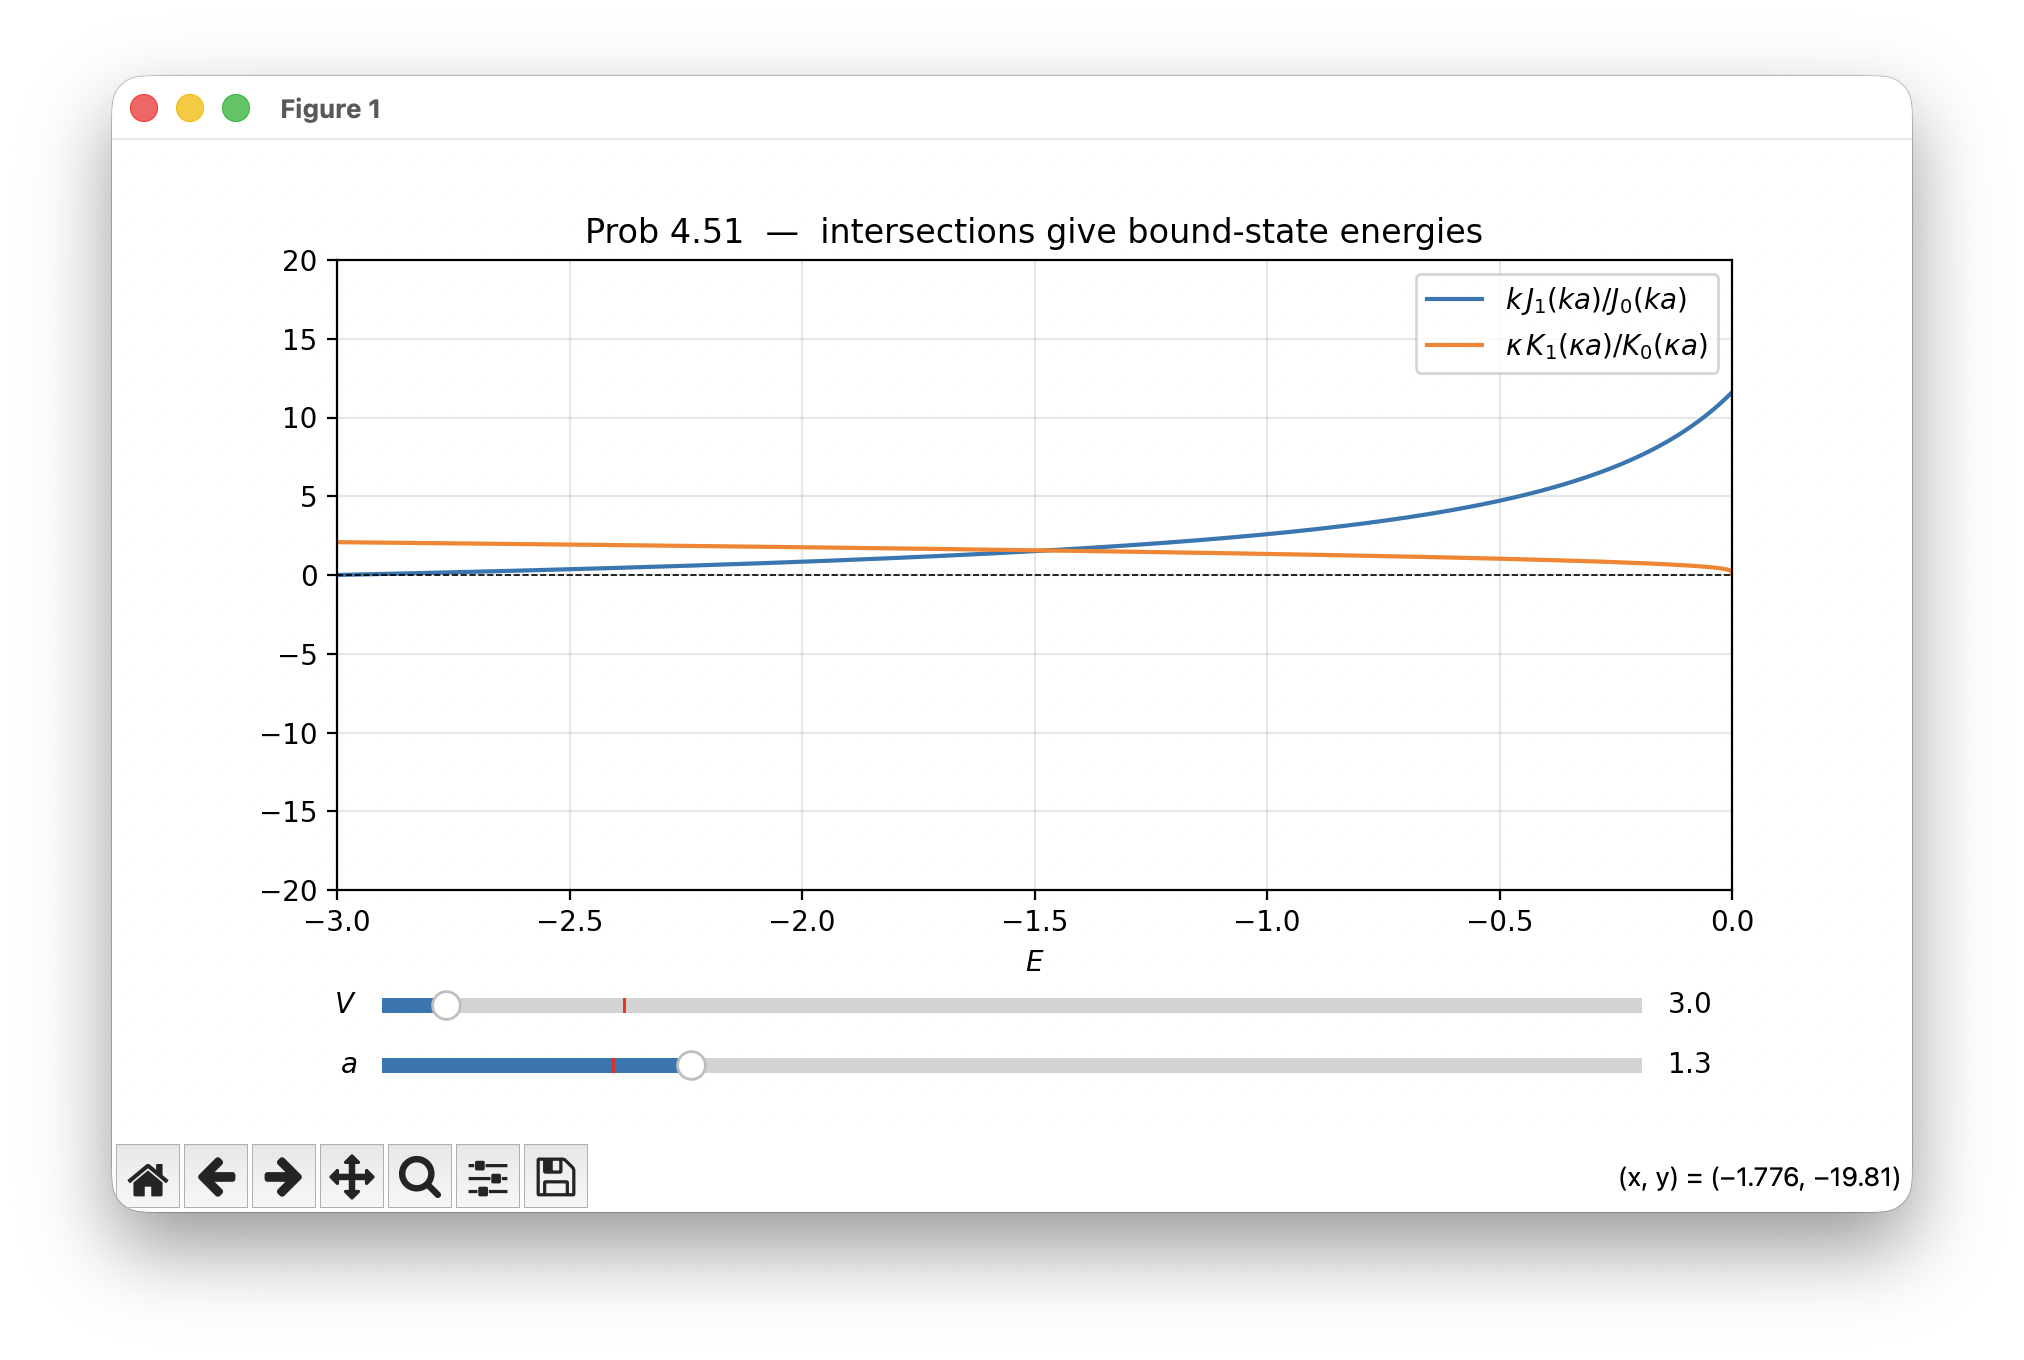
\includegraphics[width=\textwidth]{fig/prob4.51a.png}
        
        \label{fig:sub1}
    \end{subfigure}
    \hfill
    % Second subfigure
    \begin{subfigure}{0.32\textwidth}
        \centering
        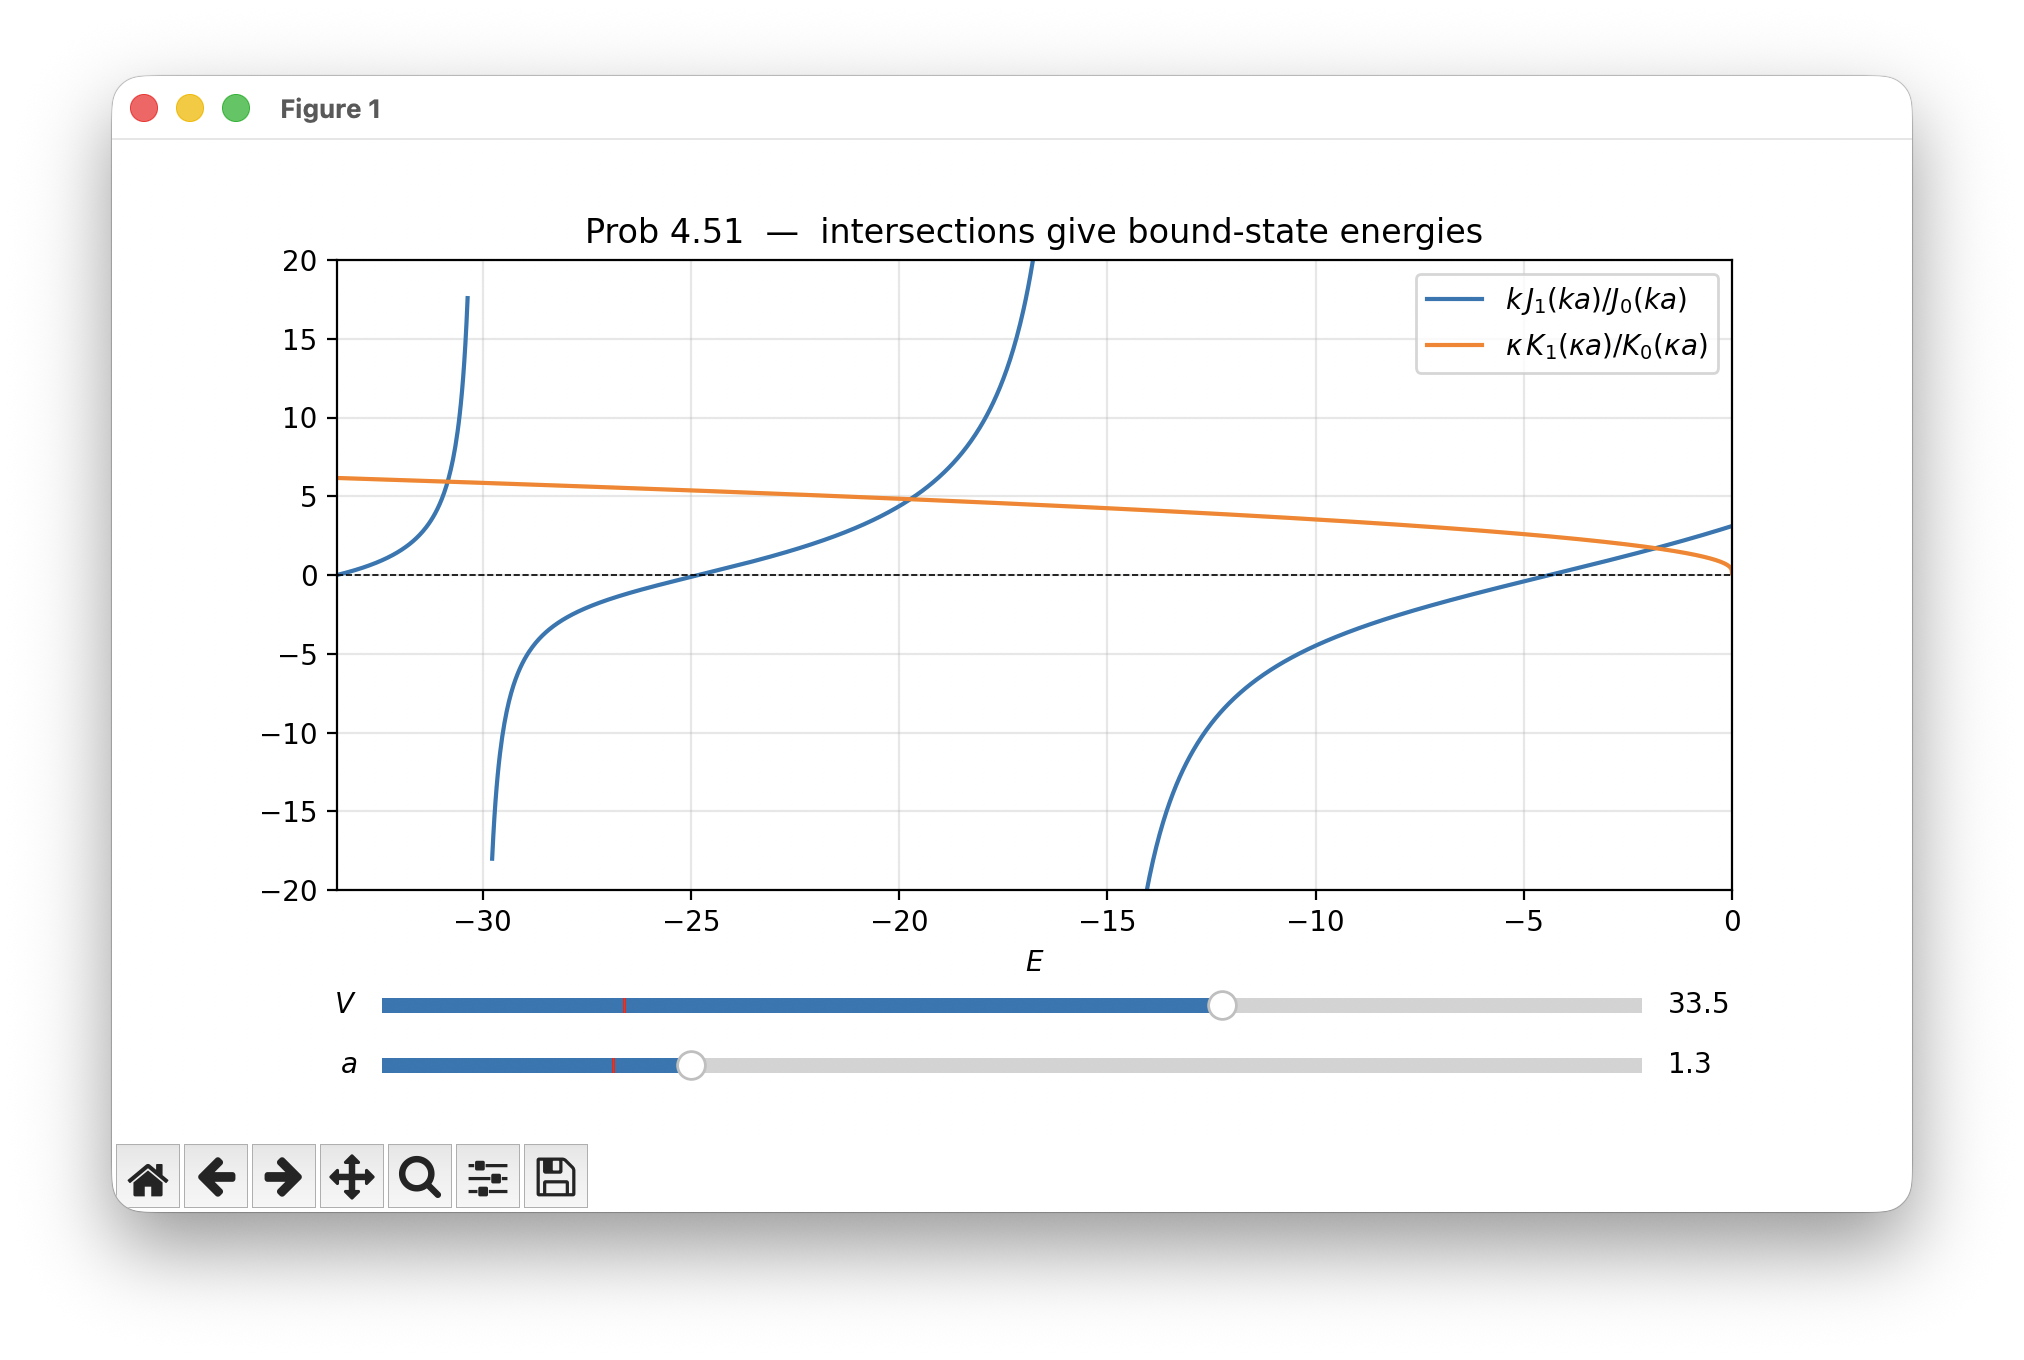
\includegraphics[width=\textwidth]{fig/prob4.51b.png}
        
        \label{fig:sub2}
    \end{subfigure}
    \hfill
    % Third subfigure
    \begin{subfigure}{0.32\textwidth}
        \centering
        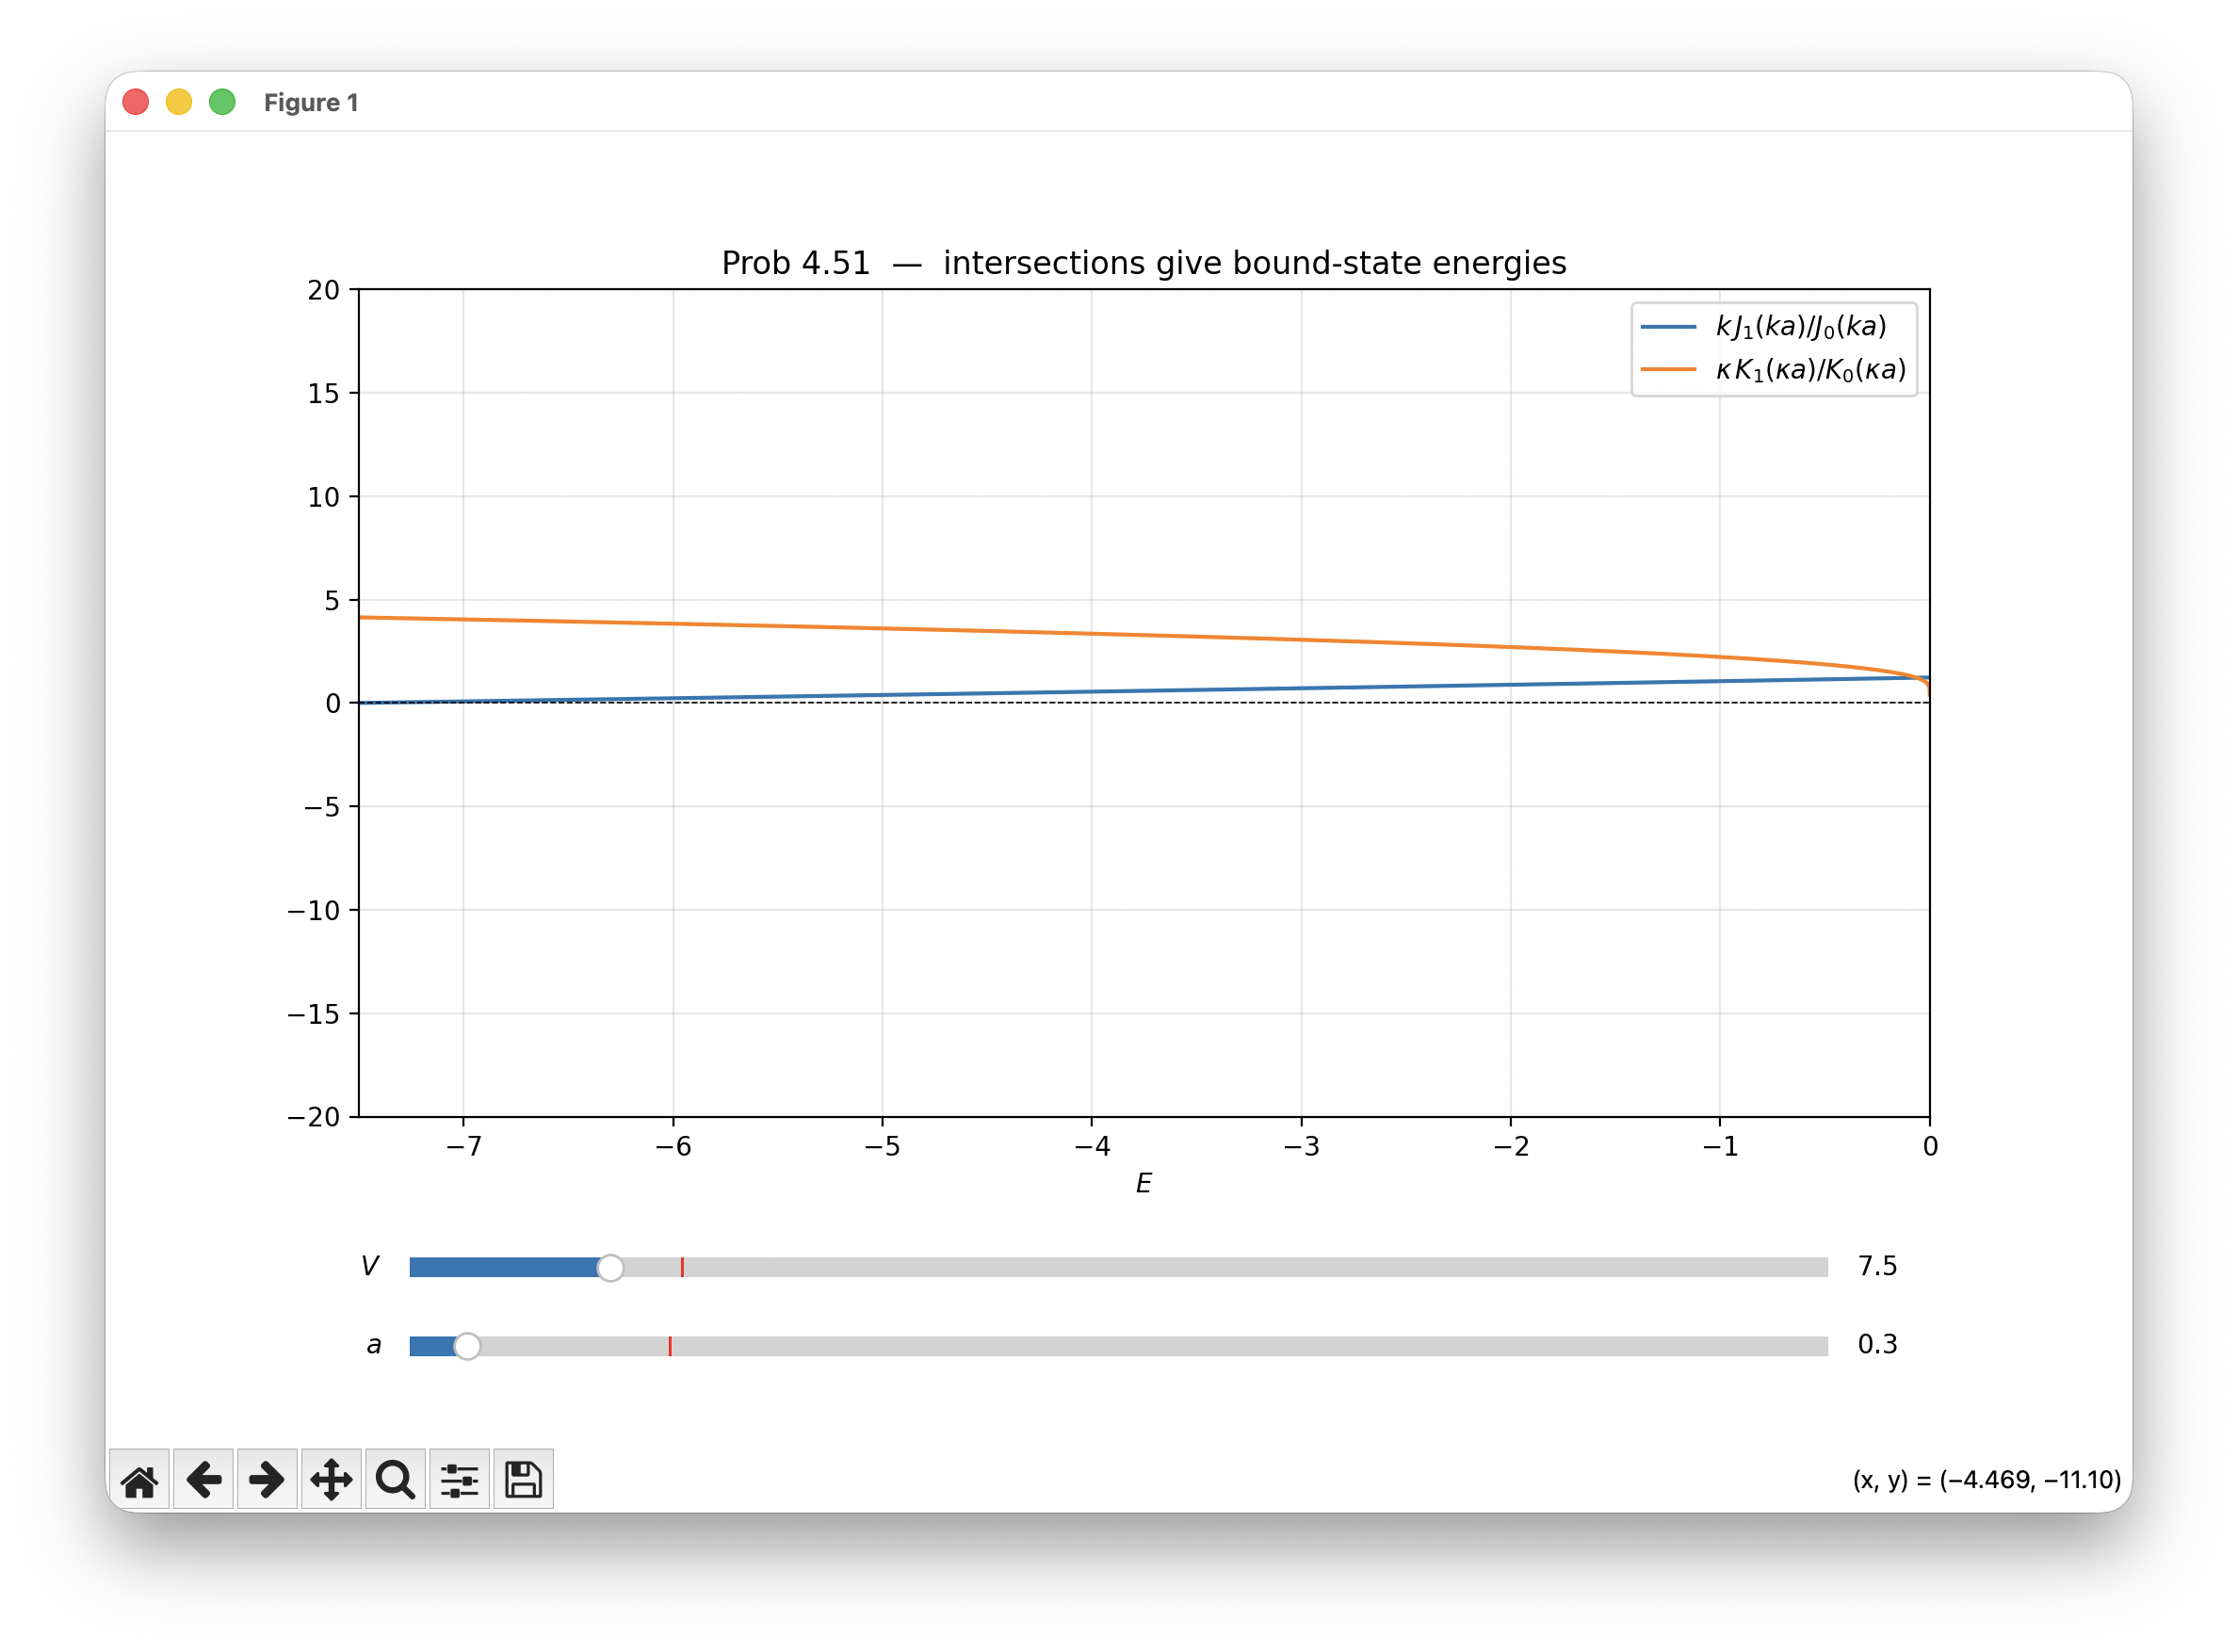
\includegraphics[width=\textwidth]{fig/prob4.51c.png}
        
        \label{fig:sub3}
    \end{subfigure}
    
    \label{fig:2dimwell}
\end{figure}
No matter how shallow or how small the potential well is, there always exists a bound state for $n=0.$
        
        \subsection*{Sol. 52}
        \begin{enumerate}
            \item 
            \begin{align*}
                \psi_{321}(r,\theta,\phi)
            =&
            -\frac{4}{81\sqrt{30}}
            a^{-3/2}
            \left(\frac{r}{a}\right)^2
            \exp(\frac{-r}{3a})
            \left(
            \frac{15}{8\pi}
            \right)^{1/2}
            \sin\theta\cos\theta 
            e^{i\phi}
            \end{align*}
            \item 
            \begin{align*}
                &\int
                \frac{16}{81^2\cdot30}
            a^{-3}
            \left(\frac{r}{a}\right)^4
            \exp(\frac{-2r}{3a})
            \left(
            \frac{15}{8\pi}
            \right)
            \sin^2\theta\cos^2\theta 
            r^2\sin\theta drd\theta d\phi\\
            =&\int 
            \frac{8r^{6} \mathrm{e}^{-\frac{2r}{3a}}}{98415 a^{7}} dr\\
            =&1
            \end{align*}
            \item 
            \begin{align*}
                \langle r^s\rangle=&\int
                \frac{8r^{6+s} \mathrm{e}^{-\frac{2r}{3a}}}{98415 a^{7}}dr\\
                =&
                -
                \frac{1}{720}
                \left(
                \frac{3a}{2}
                \right)^s\Gamma(s+7, \frac{2r}{3a})\bigg|^{\infty}_0\\
                =&\frac{1}{720}
                \left(
                \frac{3a}{2}
                \right)^s
                \Gamma(s+7).
            \end{align*}
            The gamma function is not defined on the non-positive integers, so $s$ is defined for all $\mathbb{R}$ except $s=-7,-8,\dots.$
        \end{enumerate}

        \subsection*{Sol. 53}
        \begin{enumerate}
            \item 
            $$
            \psi_{433}(r,\theta,\phi)
            =-\frac{1}{768\sqrt{35}}
            a^{-3/2}
            \left(\frac{r}{a}\right)^{3}
            \exp\left(\frac{-r}{4a}\right)
            \left(\frac{35}{64\pi}\right)^{1/2}
            \sin^3\theta e^{3i\phi}
            $$
            \item 
            \begin{align*}
                \langle r\rangle
                =&
                \frac{1}{768^2\cdot 35}
            a^{-3}
            \left(\frac{35}{64\pi}\right)
                \int 
                r
            \left(\frac{r}{a}\right)^{6}
            \exp\left(\frac{-r}{2a}\right)
            \sin^6\theta
            r^2\sin\theta  
            drd\theta d\phi \\
            =&
            \frac{1}{768^2\cdot 35}
            a^{-3}
            \left(\frac{35}{64\pi}\right)
            \frac{32}{35}
            2\pi
            \frac{1}{a^6}
                \int 
                r^9            
            \exp\left(\frac{-r}{2a}\right)
            dr\\
            =& 
            18a
            \end{align*}
            \item 
            The eigenvalue of $L^2$ is $\hbar^2l(l+1)=12\hbar^2,$ and the eigenvalue for $L_z$ is $3\hbar.$ The value I could get from $L_x^2+L_y^2$ is $3\hbar^2,$ with probability 1.
        \end{enumerate}
        \subsection*{Sol. 54}
        \begin{enumerate}
            \item $$
            \psi_{100}(r,\theta,\phi)
            =\frac{1}{\sqrt{\pi a^3}}
            e^{-r/a}
            $$
            \begin{align*}
            &\frac{1}{\pi a^3}
                \int_0^b 
                \int_0^\pi 
                \int_0^{2\pi}
                e^{-2r/a}r^2\sin\theta drd\theta 
                d\phi\\
                =&\frac{4}{a^3}
                \int_0^b 
                e^{-2r/a}r^2 dr\\
                =&
                1 - 
                (\frac{2b^2}{a^2} + \frac{2b}{a}+1)\mathrm{e}^{-\frac{2b}{a}}
            \end{align*}
            \item 
            \begin{align*}
                &1 - (\frac{1}{2}\epsilon^2 + \epsilon + 1)
                (1-\epsilon + \frac{1}{2}\epsilon^2-\frac{1}{6}\epsilon^3+\dots)\\
                \approx &
                \frac{1}{6}\epsilon^3\\
                =&\frac{4}{3}\frac{b^3}{a^3}
            \end{align*}
            \item $$
            |\psi(0)|^2
            =\frac{1}{\pi a^3}
            $$
            $$
            \frac{4}{3}\pi b^3
            \frac{1}{\pi a^3} = 
            \frac{4}{3}\frac{b^3}{a^3}
            $$
            \item 
            $$
            1.1\times 10^{-14}.
            $$
        \end{enumerate}
        \subsection*{Sol. 55}
        \begin{enumerate}
            \item 
            $$
            c_{j+1}
            =\frac{2(j+l+1-n)}{(j+1)(j+2l+2)}c_j
            $$
            $$
            c_1 = 
            \frac{2(0)}{(0+1)(0+2n)}c_0 = 0
            $$
            $$
            R_{n(n-1)}(r)
            =\frac{1}{r}\rho^{n}e^{-\rho}c_0
            =N_nr^{n-1}
            e^{-r/(an)}
            $$
            \begin{align*}
                \int_0^\infty 
                N_n^2 r^{2n-2}
                e^{-2r/(an)}r^2dr
                =N_n^2(an)^{2n+1}
                (2n)!\frac{1}{2^{2n+1}}
            \end{align*}
            $$
            N_n = \sqrt{\frac{2^{2n+1}}{(2n)!(an)^{2n+1}}}
            $$
            \item 
            \begin{align*}
                \langle r\rangle
                =& 
                \int rR_{n(n-1)}^2(Y_{(n-1)}^m)^2r^2\sin\theta dr d\theta d\phi\\
                =&
                \frac{2^{2n+1}}{(2n)!(an)^{2n+1}}
                \int r^{2n+1}e^{-2r/(an)}dr\\
                =& 
                \frac{2^{2n+1}}{(2n)!(an)^{2n+1}}
                \frac{(2n+1)!(an)^{2n+2}}{2^{2n+2}}\\
                =&\frac{(an)(2n+1)}{2}
            \end{align*}
            \begin{align*}
                \langle r^2\rangle
                =& 
                \int r^2R_{n(n-1)}^2(Y_{(n-1)}^m)^2r^2\sin\theta dr d\theta d\phi\\
                =&
                \frac{2^{2n+1}}{(2n)!(an)^{2n+1}}
                \int r^{2n+2}e^{-2r/(an)}dr\\
                =& 
                \frac{2^{2n+1}}{(2n)!(an)^{2n+1}}
                \frac{(2n+2)!(an)^{2n+3}}{2^{2n+3}}\\
                =&\frac{(an)^2(2n+1)(2n+2)}{4}
            \end{align*}
            \item 
            \begin{align*}
                \sigma_r = &
            \sqrt{\frac{(an)^2(2n+1)(2n+2)}{4}
            -\frac{(an)^2(2n+1)^2}{4}}\\
            =&\sqrt{\frac{(an)^2(2n+1)}{4}}\\
            =&\frac{\langle r\rangle}{\sqrt{(2n+1)}}
            \end{align*}
        \end{enumerate}

        \subsection*{Sol. 56}
        $$
        \{9, 5\},\;
        \{90, 6\}
        $$
        $$
        \{7, 5\},\;
        \{35, 7\}
        $$
        $$
        \{9, 6\},\;
        \{72, 8\}
        $$

        \subsection*{Sol. 57}
        \begin{enumerate}
            \item By 3.62,
            $$
            \sigma_A^2\sigma_B^2\geq 
            \left(
            \frac{1}{2i}
            \langle[x^2, L_z]\rangle
            \right)^2
            $$
            \begin{align*}
            [x^2, L_z]=&[r^2\sin^2\theta\cos^2\phi, -i\hbar\frac{\partial}{\partial\phi}]\\
            =&-i\hbar r^2\sin^2\theta[\cos^2\phi, \frac{\partial}{\partial\phi}]\\
            =&-i\hbar r^2\sin^2\theta2\sin\phi\cos\phi\\
            =&-2i\hbar xy
        \end{align*}
        Thus
        \begin{align*}
            \sigma_A\sigma_B\geq &
            \hbar
            |\langle
            xy
            \rangle|
        \end{align*}
        \item 
        $L_z$ is a determinate observable in state $\psi_{nlm},$ so $\sigma_B=0.$
        \item In this case, $\langle xy\rangle=0.$
        \end{enumerate}

        \subsection*{Sol. 58}
        \begin{enumerate}
            \item 
            $$
            A = 3
            $$
            \item 
            $
            \frac{1}{2}\hbar 
            $
            with probability $\frac{5}{9},$ and 
            $
            \frac{-1}{2}\hbar 
            $
            with probability $\frac{4}{9}.$
            The expectation value is $\frac{1}{9}\hbar.$
            \item 
            Note that 
            $$
            \frac{1}{3}
            \begin{pmatrix}
                1-2i\\
                2
            \end{pmatrix}
            =
            \frac{3-2i}{3\sqrt{2}}
            \begin{pmatrix}
                \frac{1}{\sqrt{2}}\\
                \frac{1}{\sqrt{2}}
            \end{pmatrix}
            +
            \frac{-1-2i}{3\sqrt{2}}
            \begin{pmatrix}
                \frac{1}{\sqrt{2}}\\
                \frac{-1}{\sqrt{2}}
            \end{pmatrix}
            $$
            $
            \frac{1}{2}\hbar 
            $
            with probability $\frac{13}{18},$ and 
            $
            \frac{-1}{2}\hbar 
            $
            with probability $\frac{5}{18}.$
            The expectation value is $\frac{4}{9}\hbar.$
            \item 
            Note that 
            $$
            \frac{1}{3}
            \begin{pmatrix}
                1-2i\\
                2
            \end{pmatrix}
            =
            \frac{1-4i}{3\sqrt{2}}
            \begin{pmatrix}
                \frac{1}{\sqrt{2}}\\
                \frac{i}{\sqrt{2}}
            \end{pmatrix}
            +
            \frac{i}{3\sqrt{2}}
            \begin{pmatrix}
                \frac{-i}{\sqrt{2}}\\
                \frac{-1}{\sqrt{2}}
            \end{pmatrix}
            $$
            $
            \frac{1}{2}\hbar 
            $
            with probability $\frac{17}{18},$ and 
            $
            \frac{-1}{2}\hbar 
            $
            with probability $\frac{1}{18}.$
            The expectation value is $\frac{8}{9}\hbar.$
        \end{enumerate}

        \subsection*{Sol. 59}
        \begin{align*}
            \langle S_a^{(1)}S_b^{(2)}\rangle= & 
            \frac{1}{2}
            \langle \updownarrows - \downuparrows, 
            S_a^{(1)}S_b^{(2)}
            (\updownarrows - \downuparrows)
            \rangle\\
            =&
            \frac{1}{2}
            \langle S_a^{(1)}\updownarrows, S_b^{(2)}\updownarrows\rangle
            -\frac{1}{2}
            \langle S_a^{(1)}\updownarrows, S_b^{(2)}\downuparrows\rangle
            -\frac{1}{2}
            \langle S_a^{(1)}\downuparrows, S_b^{(2)}\updownarrows\rangle
            +\frac{1}{2}
            \langle S_a^{(1)}\downuparrows, S_b^{(2)}\downuparrows\rangle
        \end{align*}
        By prob4.33
        \begin{align*}
            S_r = \frac{\hbar}{2}
            \begin{pmatrix}
                \cos\theta_r & \sin\theta_r e^{-i\phi_r}\\
                \sin\theta_r e^{i\phi_r} & -\cos\theta_r
            \end{pmatrix}
        \end{align*}
        \begin{align*}
            \langle S_a^{(1)}\updownarrows, S_b^{(2)}\updownarrows\rangle = & 
            \frac{\hbar^2}{4}
            \langle
            \cos\theta_a\updownarrows + 
            \sin\theta_ae^{i\phi_a}\downdownarrows
            ,
            \sin\theta_b e^{-i\phi_b}\upuparrows -
            \cos\theta_b\updownarrows
            \rangle\\
            =&-\frac{\hbar^2}{4}\cos\theta_a\cos\theta_b
        \end{align*}
        \begin{align*}
            \langle S_a^{(1)}\updownarrows, S_b^{(2)}\downuparrows\rangle = & 
            \frac{\hbar^2}{4}
            \langle
            \cos\theta_a\updownarrows + 
            \sin\theta_ae^{i\phi_a}\downdownarrows
            ,
            \cos\theta_b \downuparrows +
            \sin\theta_be^{i\phi_b}\downdownarrows
            \rangle\\
            =&\frac{\hbar^2}{4}\sin\theta_ae^{-i\phi_a}\sin\theta_be^{i\phi_b}
        \end{align*}
        \begin{align*}
            \langle S_a^{(1)}\downuparrows, S_b^{(2)}\updownarrows\rangle = & 
            \frac{\hbar^2}{4}
            \langle
            \sin\theta_ae^{-i\phi_a} \upuparrows -
            \cos\theta_a\downuparrows
            ,
            \sin\theta_b e^{-i\phi_b}\upuparrows -
            \cos\theta_b\updownarrows
            \rangle\\
            =&\frac{\hbar^2}{4}\sin\theta_ae^{i\phi_a}\sin\theta_be^{-i\phi_b}
        \end{align*}
        \begin{align*}
            \langle S_a^{(1)}\downuparrows, S_b^{(2)}\downuparrows\rangle = & 
            \frac{\hbar^2}{4}
            \langle
            \sin\theta_ae^{-i\phi_a} \upuparrows -
            \cos\theta_a\downuparrows
            ,
            \cos\theta_b \downuparrows +
            \sin\theta_be^{i\phi_b}\downdownarrows
            \rangle\\
            =&-\frac{\hbar^2}{4}\cos\theta_a\cos\theta_b
        \end{align*}
        \begin{align*}
            \langle S_a^{(1)}S_b^{(2)}\rangle=&
            -\frac{\hbar^2}{4}\cos\theta_a\cos\theta_b
            -\frac{\hbar^2}{4}\sin\theta_a\sin\theta_b\cos(\phi_a-\phi_b)\\
            =&-\frac{\hbar^2}{4}\bm a_z\bm b_z
            -\frac{\hbar^2}{4}\bm a_x\bm b_x - 
            \frac{\hbar^2}{4}\bm a_y\bm b_y \\
            =&-\frac{\hbar^2}{4}\cos\theta
        \end{align*}
        \subsection*{Sol. 60}
        \begin{enumerate}
        \item 
        
        \begin{align*}
            S_x^{(1)}\bigg|\frac{1}{2}\frac{1}{2}\bigg\rangle
            S_x^{(2)}\bigg|s_2\left(m-\frac{1}{2}\right)\bigg\rangle
            =&\frac{\hbar}{2}\bigg|\frac{1}{2}\frac{-1}{2}\bigg\rangle
            \frac{1}{2}\bigg(
            \hbar\sqrt{s_2(s_2+1)-(m-\frac{1}{2})(m+\frac{1}{2})}
            \bigg|s_2\left(m+\frac{1}{2}\right)\bigg\rangle
            \\&+
            \hbar\sqrt{s_2(s_2+1)-(m-\frac{1}{2})(m-\frac{3}{2})}
            \bigg|s_2\left(m-\frac{3}{2}\right)\bigg\rangle
            \bigg)
        \end{align*}
        \begin{align*}
            S_y^{(1)}\bigg|\frac{1}{2}\frac{1}{2}\bigg\rangle
            S_y^{(2)}\bigg|s_2\left(m-\frac{1}{2}\right)\bigg\rangle
            =&\frac{\hbar}{2}\bigg|\frac{1}{2}\frac{-1}{2}\bigg\rangle
            \frac{1}{2}\bigg(
            \hbar\sqrt{s_2(s_2+1)-(m-\frac{1}{2})(m+\frac{1}{2})}
            \bigg|s_2\left(m+\frac{1}{2}\right)\bigg\rangle
            \\&-
            \hbar\sqrt{s_2(s_2+1)-(m-\frac{1}{2})(m-\frac{3}{2})}
            \bigg|s_2\left(m-\frac{3}{2}\right)\bigg\rangle
            \bigg)
        \end{align*}
        \begin{align*}
            S_z^{(1)}\bigg|\frac{1}{2}\frac{1}{2}\bigg\rangle
            S_z^{(2)}\bigg|s_2\left(m-\frac{1}{2}\right)\bigg\rangle
            =&\frac{\hbar}{2}\bigg|\frac{1}{2}\frac{1}{2}\bigg\rangle
            \hbar\left(m-\frac{1}{2}\right)
            \bigg|s_2\left(m-\frac{1}{2}\right)\bigg\rangle
        \end{align*}
        \begin{align*}
            \bm S^{(1)}\bm S^{(2)}\bigg|\frac{1}{2}\frac{1}{2}\bigg\rangle
            \bigg|s_2\left(m-\frac{1}{2}\right)\bigg\rangle
            =&\\
            \frac{\hbar^2}{2}\sqrt{s_2(s_2+1)-(m-\frac{1}{2})(m+\frac{1}{2})}\bigg|\frac{1}{2}\frac{-1}{2}\bigg\rangle
            \bigg|s_2\left(m+\frac{1}{2}\right)\bigg\rangle
            +
            \frac{\hbar^2}{2}
            \left(m-\frac{1}{2}\right)
            \bigg|\frac{1}{2}\frac{1}{2}\bigg\rangle
            \bigg|s_2\left(m-\frac{1}{2}\right)\bigg\rangle
        \end{align*}
        \begin{align*}
            &S^2\bigg|\frac{1}{2}\frac{1}{2}\bigg\rangle
            \bigg|s_2\left(m-\frac{1}{2}\right)\bigg\rangle
            =\hbar^2\frac{3}{4}\bigg|\frac{1}{2}\frac{1}{2}\bigg\rangle
            \bigg|s_2\left(m-\frac{1}{2}\right)\bigg\rangle
            +
            \hbar^2s_2(s_2+1)\bigg|\frac{1}{2}\frac{1}{2}\bigg\rangle
            \bigg|s_2\left(m-\frac{1}{2}\right)\bigg\rangle\\
            &+\hbar^2\sqrt{s_2(s_2+1)-(m-\frac{1}{2})(m+\frac{1}{2})}\bigg|\frac{1}{2}\frac{-1}{2}\bigg\rangle
            \bigg|s_2\left(m+\frac{1}{2}\right)\bigg\rangle
            +
            \hbar^2
            \left(m-\frac{1}{2}\right)
            \bigg|\frac{1}{2}\frac{1}{2}\bigg\rangle
            \bigg|s_2\left(m-\frac{1}{2}\right)\bigg\rangle\\
            =&\hbar^2\sqrt{s_2(s_2+1)-(m-\frac{1}{2})(m+\frac{1}{2})}\bigg|\frac{1}{2}\frac{-1}{2}\bigg\rangle
            \bigg|s_2\left(m+\frac{1}{2}\right)\bigg\rangle\\
            &+
            \hbar^2(s_2(s_2+1)+m+\frac{1}{4})
            \bigg|\frac{1}{2}\frac{1}{2}\bigg\rangle
            \bigg|s_2\left(m-\frac{1}{2}\right)\bigg\rangle
        \end{align*}
        
        \begin{align*}
            S_x^{(1)}\bigg|\frac{1}{2}\frac{-1}{2}\bigg\rangle
            S_x^{(2)}\bigg|s_2\left(m+\frac{1}{2}\right)\bigg\rangle
            =&\frac{\hbar}{2}\bigg|\frac{1}{2}\frac{1}{2}\bigg\rangle
            \frac{1}{2}\bigg(
            \hbar\sqrt{s_2(s_2+1)-(m+\frac{1}{2})(m+\frac{3}{2})}
            \bigg|s_2\left(m+\frac{3}{2}\right)\bigg\rangle
            \\&+
            \hbar\sqrt{s_2(s_2+1)-(m+\frac{1}{2})(m-\frac{1}{2})}
            \bigg|s_2\left(m-\frac{1}{2}\right)\bigg\rangle
            \bigg)
        \end{align*}
        \begin{align*}
            S_y^{(1)}\bigg|\frac{1}{2}\frac{-1}{2}\bigg\rangle
            S_y^{(2)}\bigg|s_2\left(m+\frac{1}{2}\right)\bigg\rangle
            =&-\frac{\hbar}{2}\bigg|\frac{1}{2}\frac{1}{2}\bigg\rangle
            \frac{1}{2}\bigg(
            \hbar\sqrt{s_2(s_2+1)-(m+\frac{1}{2})(m+\frac{3}{2})}
            \bigg|s_2\left(m+\frac{3}{2}\right)\bigg\rangle
            \\&-
            \hbar\sqrt{s_2(s_2+1)-(m+\frac{1}{2})(m-\frac{1}{2})}
            \bigg|s_2\left(m-\frac{1}{2}\right)\bigg\rangle
            \bigg)
        \end{align*}
        \begin{align*}
            S_z^{(1)}\bigg|\frac{1}{2}\frac{-1}{2}\bigg\rangle
            S_z^{(2)}\bigg|s_2\left(m+\frac{1}{2}\right)\bigg\rangle
            =&\frac{-\hbar}{2}\bigg|\frac{1}{2}\frac{-1}{2}\bigg\rangle
            \hbar\left(m+\frac{1}{2}\right)
            \bigg|s_2\left(m+\frac{1}{2}\right)\bigg\rangle
        \end{align*}

        \begin{align*}
            \bm S^{(1)}\bm S^{(2)}\bigg|\frac{1}{2}\frac{-1}{2}\bigg\rangle
            \bigg|s_2\left(m+\frac{1}{2}\right)\bigg\rangle
            =&\\
            \frac{\hbar^2}{2}\sqrt{s_2(s_2+1)-(m+\frac{1}{2})(m-\frac{1}{2})}\bigg|\frac{1}{2}\frac{1}{2}\bigg\rangle
            \bigg|s_2\left(m-\frac{1}{2}\right)\bigg\rangle
            -
            \frac{\hbar^2}{2}
            \left(m+\frac{1}{2}\right)
            \bigg|\frac{1}{2}\frac{-1}{2}\bigg\rangle
            \bigg|s_2\left(m+\frac{1}{2}\right)\bigg\rangle
        \end{align*}
        \begin{align*}
            &S^2\bigg|\frac{1}{2}\frac{-1}{2}\bigg\rangle
            \bigg|s_2\left(m+\frac{1}{2}\right)\bigg\rangle
            =\hbar^2\frac{3}{4}\bigg|\frac{1}{2}\frac{-1}{2}\bigg\rangle
            \bigg|s_2\left(m+\frac{1}{2}\right)\bigg\rangle
            +
            \hbar^2s_2(s_2+1)\bigg|\frac{1}{2}\frac{-1}{2}\bigg\rangle
            \bigg|s_2\left(m+\frac{1}{2}\right)\bigg\rangle\\
            &+\hbar^2\sqrt{s_2(s_2+1)-(m-\frac{1}{2})(m+\frac{1}{2})}\bigg|\frac{1}{2}\frac{1}{2}\bigg\rangle
            \bigg|s_2\left(m-\frac{1}{2}\right)\bigg\rangle
            -
            \hbar^2
            \left(m+\frac{1}{2}\right)
            \bigg|\frac{1}{2}\frac{-1}{2}\bigg\rangle
            \bigg|s_2\left(m+\frac{1}{2}\right)\bigg\rangle\\
            =&\hbar^2\sqrt{s_2(s_2+1)-(m-\frac{1}{2})(m+\frac{1}{2})}\bigg|\frac{1}{2}\frac{1}{2}\bigg\rangle
            \bigg|s_2\left(m-\frac{1}{2}\right)\bigg\rangle\\
            &+
            \hbar^2(s_2(s_2+1)-m+\frac{1}{4})
            \bigg|\frac{1}{2}\frac{-1}{2}\bigg\rangle
            \bigg|s_2\left(m+\frac{1}{2}\right)\bigg\rangle
        \end{align*}
        
        \begin{align*}
            s(s+1)A = (s_2(s_2+1)+m+\frac{1}{4})A + \sqrt{s_2(s_2+1)-(m-\frac{1}{2})(m+\frac{1}{2})}B
        \end{align*}
        \begin{align*}
            s(s+1)B = \sqrt{s_2(s_2+1)-(m-\frac{1}{2})(m+\frac{1}{2})}A + (s_2(s_2+1)-m+\frac{1}{4})B
        \end{align*}
        Let $a=s_2(s_2+1)+\frac{1}{4},$ $b=\sqrt{s_2(s_2+1)-(m-\frac{1}{2})(m+\frac{1}{2})},$ then
        $$
        \frac{A}{B} = \frac{(a+m)A + bB}{bA + (a-m)B}
        $$
        $$
        b(\frac{A}{B})^2 + (-2m)\frac{A}{B} - b= 0
        $$
        $$
        \frac{A}{B} = \frac{2m\pm\sqrt{4m^2+4b^2}}{2b}
    =   \frac{m\pm\sqrt{s_2(s_2+1)+\frac{1}{4}}}{\sqrt{s_2(s_2+1)-m^2+\frac{1}{4}}} = \frac{m\pm(s_2+\frac{1}{2})}{\sqrt{(s_2+\frac{1}{2})^2-m^2}}
        $$
If plus, then 
$$
\frac{A}{B} = \sqrt{\frac{s_2+\frac{1}{2}+m}{s_2+\frac{1}{2}-m}},
$$
if minus, then 
$$
\frac{A}{B} = -\sqrt{\frac{s_2+\frac{1}{2}-m}{s_2+\frac{1}{2}+m}}.
$$
Combine with the fact that $A^2+B^2=1,$ we have 
$$
B = \pm\sqrt{\frac{s_2+\frac{1}{2}\mp m}{2s_2+1}}, 
A = \sqrt{\frac{s_2+\frac{1}{2}\pm m}{2s_2+1}}.
$$
\item 
    $$
    |10\rangle =
    \sqrt{\frac{\frac{1}{2}+\frac{1}{2}}{2\cdot 
    \frac{1}{2} + 1}}
    |\frac{1}{2}\frac{1}{2}
    \frac{1}{2}\frac{-1}{2}\rangle
    +
    \sqrt{\frac{\frac{1}{2}+\frac{1}{2}}{2\cdot 
    \frac{1}{2} + 1}}
    |\frac{1}{2}\frac{1}{2}
    \frac{-1}{2}\frac{1}{2}\rangle
    =
    \sqrt{\frac{1}{2}}
   |\frac{1}{2}\frac{1}{2}
    \frac{1}{2}\frac{-1}{2}\rangle
    +
    \sqrt{\frac{1}{2}}
    |\frac{1}{2}\frac{1}{2}
    \frac{-1}{2}\frac{1}{2}\rangle
    $$
    $$
    |\frac{3}{2}\frac{-1}{2}\rangle =
    \sqrt{\frac{1+\frac{1}{2}+\frac{1}{2}}{2\cdot 
    1 + 1}}
    |1\frac{1}{2}
    0\frac{-1}{2}\rangle
    +
    \sqrt{\frac{1+\frac{1}{2}-\frac{1}{2}}{2\cdot 
    1 + 1}}
    |1\frac{1}{2}
    (-1)\frac{1}{2}\rangle
    =
    \sqrt{\frac{2}{3}}
    |1\frac{1}{2}
    0\frac{-1}{2}\rangle
    +
    \sqrt{\frac{1}{3}}
    |1\frac{1}{2}
    (-1)\frac{1}{2}\rangle
    $$
    $$
    |\frac{3}{2}\frac{1}{2}\rangle =
    -\sqrt{\frac{2+\frac{1}{2}+\frac{1}{2}}{2\cdot 
    2 + 1}}
    |2\frac{1}{2}
    1\frac{-1}{2}\rangle
    +
    \sqrt{\frac{2+\frac{1}{2}-\frac{1}{2}}
    {2\cdot 2 + 1}}
    |2\frac{1}{2}
    0\frac{1}{2}\rangle
    =
    -\sqrt{\frac{3}{5}}
    |2\frac{1}{2}
    1\frac{-1}{2}\rangle
    +
    \sqrt{\frac{2}{5}}
    |2\frac{1}{2}
    0\frac{1}{2}\rangle
    $$
\end{enumerate}
\subsection*{Sol. 61}
$$
S_+ \chi_{-3/2}
=\hbar\sqrt{(\frac{3}{2}\frac{5}{2} - (-\frac{3}{2})(-\frac{1}{2}))} \chi_{-1/2}
=\hbar\sqrt{3}\chi_{-1/2}
$$
$$
S_+ \chi_{-1/2}
=\hbar\sqrt{(\frac{3}{2}\frac{5}{2} - (-\frac{1}{2})(\frac{1}{2}))} \chi_{1/2}
=\hbar2\chi_{1/2}
$$
$$
S_+ \chi_{1/2}
=\hbar\sqrt{(\frac{3}{2}\frac{5}{2} - (\frac{1}{2})(\frac{3}{2}))} \chi_{3/2}
=\hbar\sqrt{3}\chi_{3/2}
$$
$$
S_- \chi_{3/2}
=\hbar\sqrt{(\frac{3}{2}\frac{5}{2} - (\frac{3}{2})(\frac{1}{2}))} \chi_{1/2}
=\hbar\sqrt{3}\chi_{1/2}
$$
$$
S_- \chi_{1/2}
=\hbar\sqrt{(\frac{3}{2}\frac{5}{2} - (\frac{1}{2})(-\frac{1}{2}))} \chi_{-1/2}
=\hbar2\chi_{-1/2}
$$
$$
S_- \chi_{-1/2}
=\hbar\sqrt{(\frac{3}{2}\frac{5}{2} - (-\frac{1}{2})(-\frac{3}{2}))} \chi_{-3/2}
=\hbar\sqrt{3}\chi_{-3/2}
$$
\begin{align*}
    &S_+ = \hbar\begin{pmatrix}
        0 & \sqrt{3} & 0  & 0\\
        0 & 0 & 2  & 0\\
        0 & 0 & 0  & \sqrt{3}\\
        0 & 0 & 0  & 0\\
    \end{pmatrix}\\
    &S_- = \hbar\begin{pmatrix}
        0 & 0 & 0  & 0\\
        \sqrt{3} & 0 & 0  & 0\\
        0 & 2 & 0  & 0\\
        0 & 0 & \sqrt{3}  & 0\\
    \end{pmatrix}\\
    &S_x = \frac{\hbar}{2}
    \begin{pmatrix}
        0 & \sqrt{3} & 0  & 0\\
        \sqrt{3} & 0 & 2  & 0\\
        0 & 2 & 0  & \sqrt{3}\\
        0 & 0 & \sqrt{3}  & 0\\
    \end{pmatrix}
\end{align*}
Characteristic equation:
\begin{align*}
    ch_T(t) = (t-\frac{\hbar}{2})
    (t+\frac{\hbar}{2})
    (t-\frac{3\hbar}{2})
    (t+\frac{3\hbar}{2})
\end{align*}
\subsection*{Sol. 62}
Let $v_s, v_{s-1},\dots, v_{-s}$ be a basis of a spin $s$ system. Then 
$$
S_zv_j = \hbar j v_j.
$$
$$
S_+v_j 
= \hbar \sqrt{s(s+1)-j(j+1)}v_{j+1}
=\hbar \sqrt{(s+j+1)(s-j)}v_{j+1}
=\hbar b_{j+1}v_{j+1}.
$$
$$
S_-v_j = \hbar \sqrt{s(s+1)-j(j-1)}v_{j-1}
=\hbar \sqrt{(s+j)(s-j+1)}v_{j-1}=\hbar b_jv_j.
$$

\begin{align*}
    S_xv_j = \frac{\hbar}{2}(b_{j+1}v_{j+1} + b_j v_j)
\end{align*}
\begin{align*}
    S_yv_j = \frac{\hbar}{2i}(b_{j+1}v_{j+1} - b_j v_j)
\end{align*}

\subsection*{Sol. 63}
\begin{align*}
    L_+Y^m_l=&\hbar\sqrt{(l-m)(l+m+1)}
    K^{m+1}_le^{i(m+1)\phi}P^{m+1}_l(\cos\theta)\\
    =&\hbar e^{i\phi}(\frac{\partial}{\partial\theta}+i\cot\theta\frac{\partial}{\partial\phi})
    K^m_le^{im\phi}P^m_l(\cos\theta)\\
    =&\hbar e^{i\phi}K^m_l
    (e^{im\phi}P^{m'}_l(\cos\theta)(-\sin\theta)
    +i\cot\theta P^{m}_l(\cos\theta)(im)e^{im\phi})\\
    =&\hbar e^{i(m+1)\phi}K^m_l
    (-\sin\theta (-\frac{\sqrt{1-\cos^2\theta}}{1-\cos^2\theta}P^{m+1}_l(\cos\theta) - 
    m\frac{\cos\theta}{1-\cos^2\theta}P^m_l(\cos\theta))
    -m\cot\theta P^{m}_l(\cos\theta))\\
    =&\hbar e^{i(m+1)\phi}K_l^mP^{m+1}_l(\cos\theta).
\end{align*}
We obtain the relation
$$
\sqrt{(l-m)(l+m+1)}K_l^{m+1} = K^m_l,
$$
and thus we have $ \sqrt{\frac{(l+m)!}{(l-m)!}}K^m_l =K^0_l.$
By problem 4.25,
\begin{align*}
    K^{l}_lP^l_l(\cos\theta)
    =
    \frac{1}{\sqrt{(2l)!}}K^0_l
    (-1)^l\sin^l\theta \frac{(2l)!}{2^l l!}=(-1)^l\sqrt{\frac{(2l+1)!}{\pi}}\frac{1}{2^{l+1}l!}\sin^l\theta.
\end{align*}
\begin{align*}
    K^0_l = 
    \sqrt{\frac{(2l+1)}{\pi}}\frac{1}{2}
\end{align*}
\begin{align*}
    K^m_l 
    =\sqrt{\frac{(2l+1)}{4\pi}
    \frac{(l-m)!}{(l+m)!}}.
\end{align*}

\subsection*{Sol. 64}
\begin{enumerate}
    \item $2\hbar^2$ with probability 1.
    \item $0$ with probability $\frac{1}{3}$, 
    $\hbar$ with probability $\frac{2}{3}$.
    \item $\frac{3}{4}\hbar^2$ with probability 1.
    \item $\frac{1}{2}\hbar$ with probability $\frac{1}{3}$, 
    $\frac{-1}{2}\hbar$  with probability $\frac{2}{3}$.
    \item 
    $$
    |10\rangle|\frac{1}{2}\frac{1}{2}\rangle = 
    \sqrt{\frac{2}{3}}|\frac{3}{2}\frac{1}{2}\rangle -
    \sqrt{\frac{1}{3}}|\frac{1}{2}\frac{1}{2}\rangle
    $$
    $$
    |11\rangle|\frac{1}{2}\frac{-1}{2}\rangle = 
    \sqrt{\frac{1}{3}}|\frac{3}{2}\frac{1}{2}\rangle +
    \sqrt{\frac{2}{3}}|\frac{1}{2}\frac{1}{2}\rangle
    $$
    The state becomes 
    $$
    \frac{2\sqrt{2}}{3}|\frac{3}{2}\frac{1}{2}\rangle +
    \frac{1}{3}|\frac{1}{2}\frac{1}{2}\rangle
    $$
    $\frac{15}{4}\hbar^2$ with probability $\frac{8}{9}$, 
    $\frac{3}{4}\hbar^2$  with probability $\frac{1}{9}$.
    \item $\frac{1}{2}\hbar$ with probability $1.$
    \item 
    The position probability density is 
    \begin{align*}
        &R_{21}^2\left|\sqrt{\frac{1}{3}}Y^0_1 + \sqrt{\frac{2}{3}}Y^1_1\right|^2r^2\sin\theta\\
        =&
        \frac{1}{24}a^{-3}\frac{r^2}{a^2}\exp(\frac{-r}{a})
        \left|\sqrt{\frac{1}{3}}\sqrt{\frac{3}{4\pi}}\cos\theta -\sqrt{\frac{2}{3}}\sqrt{\frac{3}{8\pi}}
        \sin\theta e^{i\phi}\right|^2
        r^2\sin\theta\\
        =&\frac{1}{96\pi}\frac{r^4}{a^5}
        \exp\left(\frac{-r}{a}\right)\sin\theta
        (1-2\sin2\theta\cos\phi).
        \end{align*}
        \item 
        The probability density of finding the particle with spin up at radius $r$ is 
        $$
        \frac{1}{3}\frac{1}{24}\frac{r^4}{a^5}
        \exp\left(\frac{-r}{a}\right).
        $$
\end{enumerate}

\subsection*{Sol. 65}
$$
|\frac{3}{2}\frac{3}{2}\rangle = 
|\uparrow\uparrow\uparrow\rangle
$$
\begin{align*}
    S_-|\uparrow\uparrow\uparrow\rangle
=&(S_-^{(1)}|\uparrow\rangle)|\uparrow\uparrow\rangle
+|\uparrow\rangle(S_-^{(2)}|\uparrow\rangle)|\uparrow\rangle
+
|\uparrow\uparrow\rangle(S_-^{(3)}|\uparrow\rangle)\\
=&\hbar
(|\downarrow\uparrow\uparrow\rangle + 
|\uparrow\downarrow\uparrow\rangle
+|\uparrow\uparrow\downarrow\rangle
),
\end{align*}
so 
$$
|\frac{3}{2}\frac{1}{2}\rangle = 
\frac{1}{\sqrt{3}}|\downarrow\uparrow\uparrow\rangle + 
\frac{1}{\sqrt{3}}|\uparrow\downarrow\uparrow\rangle+
\frac{1}{\sqrt{3}}|\uparrow\uparrow\downarrow\rangle
$$
\begin{align*}
    &(S_-^{(1)} + S_-^{(2)} + S_-^{(3)})
 (|\downarrow\uparrow\uparrow\rangle + 
|\uparrow\downarrow\uparrow\rangle
+|\uparrow\uparrow\downarrow\rangle
)
\propto
(|\downarrow\downarrow\uparrow\rangle + |\downarrow\uparrow\downarrow\rangle +
|\uparrow\downarrow\downarrow\rangle),
\end{align*}
so 
$$
|\frac{3}{2}\frac{-1}{2}\rangle = 
\frac{1}{\sqrt{3}}|\downarrow\downarrow\uparrow\rangle + 
\frac{1}{\sqrt{3}}|\downarrow\uparrow\downarrow\rangle+
\frac{1}{\sqrt{3}}|\uparrow\downarrow\downarrow\rangle,
$$
and 
$$
|\frac{3}{2}\frac{-3}{2}\rangle = 
|\downarrow\downarrow\downarrow\rangle.
$$
$$
|\frac{1}{2}\frac{1}{2}\rangle_1
=\frac{1}{\sqrt{2}}
(|\uparrow\downarrow\uparrow\rangle-|\downarrow\uparrow\uparrow\rangle)
$$
$$
|\frac{1}{2}\frac{-1}{2}\rangle_1
=
\frac{1}{\sqrt{2}}
(|\uparrow\downarrow\downarrow\rangle-|\downarrow\uparrow\downarrow\rangle)
$$
$$
|\frac{1}{2}\frac{1}{2}\rangle_2
=\frac{1}{\sqrt{2}}
(|\uparrow\uparrow\downarrow\rangle - |\downarrow\uparrow\uparrow\rangle)
$$
$$
|\frac{1}{2}\frac{-1}{2}\rangle_2   
=
\frac{1}{\sqrt{2}}
(|\uparrow\downarrow\downarrow\rangle - |\downarrow\downarrow\uparrow\rangle).
$$

\subsection*{Sol. 66}
By prob4.31 and by Ch3.5.1, to attain the minimum uncertainty bound, we must satisfy
\begin{align*}
    (S_y-\langle S_y\rangle)\begin{pmatrix}
        a \\ b
    \end{pmatrix}
    =ir
    (S_x-\langle S_x\rangle)\begin{pmatrix}
        a \\ b
    \end{pmatrix}
\end{align*}
for some real number $r.$
\begin{align*}
    \frac{\hbar}{2}i\begin{pmatrix}
        -b \\ a
    \end{pmatrix}
    -\frac{\hbar}{2}(-i\bar ab+i\bar ba)\begin{pmatrix}
        a\\b
    \end{pmatrix}
    =\frac{\hbar}{2}ir\begin{pmatrix}
        b\\a
    \end{pmatrix}
    -ir\frac{\hbar}{2}
    (\bar ab+\bar ba)
    \begin{pmatrix}
        a\\b
    \end{pmatrix}
\end{align*}
\begin{align*}
    -b-(-\bar ab + \bar ba)a = rb - r(\bar a b + \bar b a)a
\end{align*}
\begin{align*}
    a-(-\bar ab + \bar ba)b = ra - r(\bar a b + \bar b a)b
\end{align*}
\begin{align*}
    r = \frac{-b -(-\bar ab+\bar ba )a}{b-(\bar ab +\bar ba)a}
    =\frac{a-(-\bar a b + \bar ba)b}{a-(\bar a b + \bar ba)b}
\end{align*}
Note that 
\begin{align*}
    -ab + (\bar ab+\bar ba)b^2 - (-\bar ab+\bar ba)a^2 = ab
    -(-\bar ab+\bar ba)b^2 - (\bar ab + \bar ba)a^2
\end{align*}
\begin{align*}
    -ab + a\bar bb^2 +\bar a ba^2 = 0
\end{align*}
\begin{align*}
    ab(-1 + |b|^2 + |a|^2) = 0,
\end{align*}
these two are guaranteed to be equal.
To ensure $r$ to be real
\begin{align*}
    \frac{a-(-\bar a b + \bar ba)b}{a-(\bar a b + \bar ba)b} = 
    \frac{\bar a-(-a \bar b + b\bar a)\bar b}
    {\bar a-( a \bar b + b\bar a)\bar b}
\end{align*}
\begin{align*}
    &a\bar a - a(a\bar b + b\bar a)\bar b
    -\bar a(-\bar a b + \bar ba)b 
    +(-\bar ab + \bar ba)(a\bar b + b\bar a)b\bar b\\
    =&a\bar a - a(-a\bar b + b\bar a)\bar b -
    \bar a(\bar ab+\bar ba)b + (\bar a b+\bar ba)(-a\bar b+b\bar a)b\bar b
\end{align*}
\begin{align*}
    -a^2\bar b^2 + \bar a^2b^2 - \bar a^2b^2 b\bar b + \bar b^2a^2b\bar b = 0
\end{align*}
\begin{align*}
    (1-b\bar b)(\bar a^2 b^2 - a^2\bar b^2) = 0
\end{align*}
The condition holds when $\bar a
^2b^2$ is real.

\subsection*{Sol. 67}
\begin{enumerate}
    \item 
    \begin{align*}
        S^2 =& (\bm S_1+\bm S_2 + \bm S_3)^2\\
        =&S_1^2 + S_2^2 + S_3^2 +
        2\bm S_1\cdot \bm S_2
        +2\bm S_2\cdot \bm S_3
        +2\bm S_1\cdot \bm S_3\\
        =&\frac{9}{4}\hbar^2 + 2\frac{H}{J}
    \end{align*}
    $$
    H = \frac{J}{2}(S^2-\frac{9}{4}\hbar^2)
    $$
    \item 
    The lowest possible total spin is 
    $\frac{3}{4}\hbar^2,$ so the ground sate energy is 
    $-\frac{3}{4}\hbar^2J.$
    By problem4.65, the degeneracy is 4.
    \item 
    \begin{align*}
        &S^2 - (\bm S_1 + \bm S_3)^2 - (\bm S_2 + \bm S_4)^2\\
        =&
        S_1^2+ S_2^2 + S_3^2 + S_4^2 +
        2\bm S_1\cdot \bm S_2
        +2\bm S_1\cdot \bm S_3
        +2\bm S_1\cdot \bm S_4
        +2\bm S_2\cdot \bm S_3\\
        &+2\bm S_2\cdot \bm S_4
        +2\bm S_3\cdot \bm S_4
        -S_1^2-S_3^2-2\bm S_1\cdot \bm S_3
        -S_2^2 - S_4^2 - 2\bm S_2\cdot \bm S_4
        \\
        =&
         2\bm S_1\cdot \bm S_2
        +2\bm S_1\cdot \bm S_4
        +2\bm S_2\cdot \bm S_3
        +2\bm S_3\cdot \bm S_4
    \end{align*}
    so
    $$
    H = \frac{1}{2}J\left[S^2 - (\bm S_1+\bm S_3)^2 - (\bm S_2 + \bm S_4)^2\right]
    $$
    The ground state energy is to let the total spin 0, and the two subsystems be of spin 1, and therefore
    $-2\hbar^2J$
 \end{enumerate}
 \subsection*{Sol. 68}
 \begin{enumerate}
     \item 
     \begin{align*}
         v_j =& (-\frac{e^2}{4\pi\epsilon_0}\frac{1}{bj/(N+1)}
         +\frac{\hbar^2}{2m_e}\frac{l(l+1)}{(bj/(N+1))^2})\frac{2m_e(b/(N+1))^2}{\hbar^2}\\
         =&
          -\frac{e^22m_e}{4\pi\epsilon_0\hbar^2}
          \frac{b}{j(N+1)}
          +\frac{l(l+1)}{j^2}\\
          =&-\frac{2b}{ja(N+1)} + \frac{l(l+1)}{j^2}
     \end{align*}
     \item 
     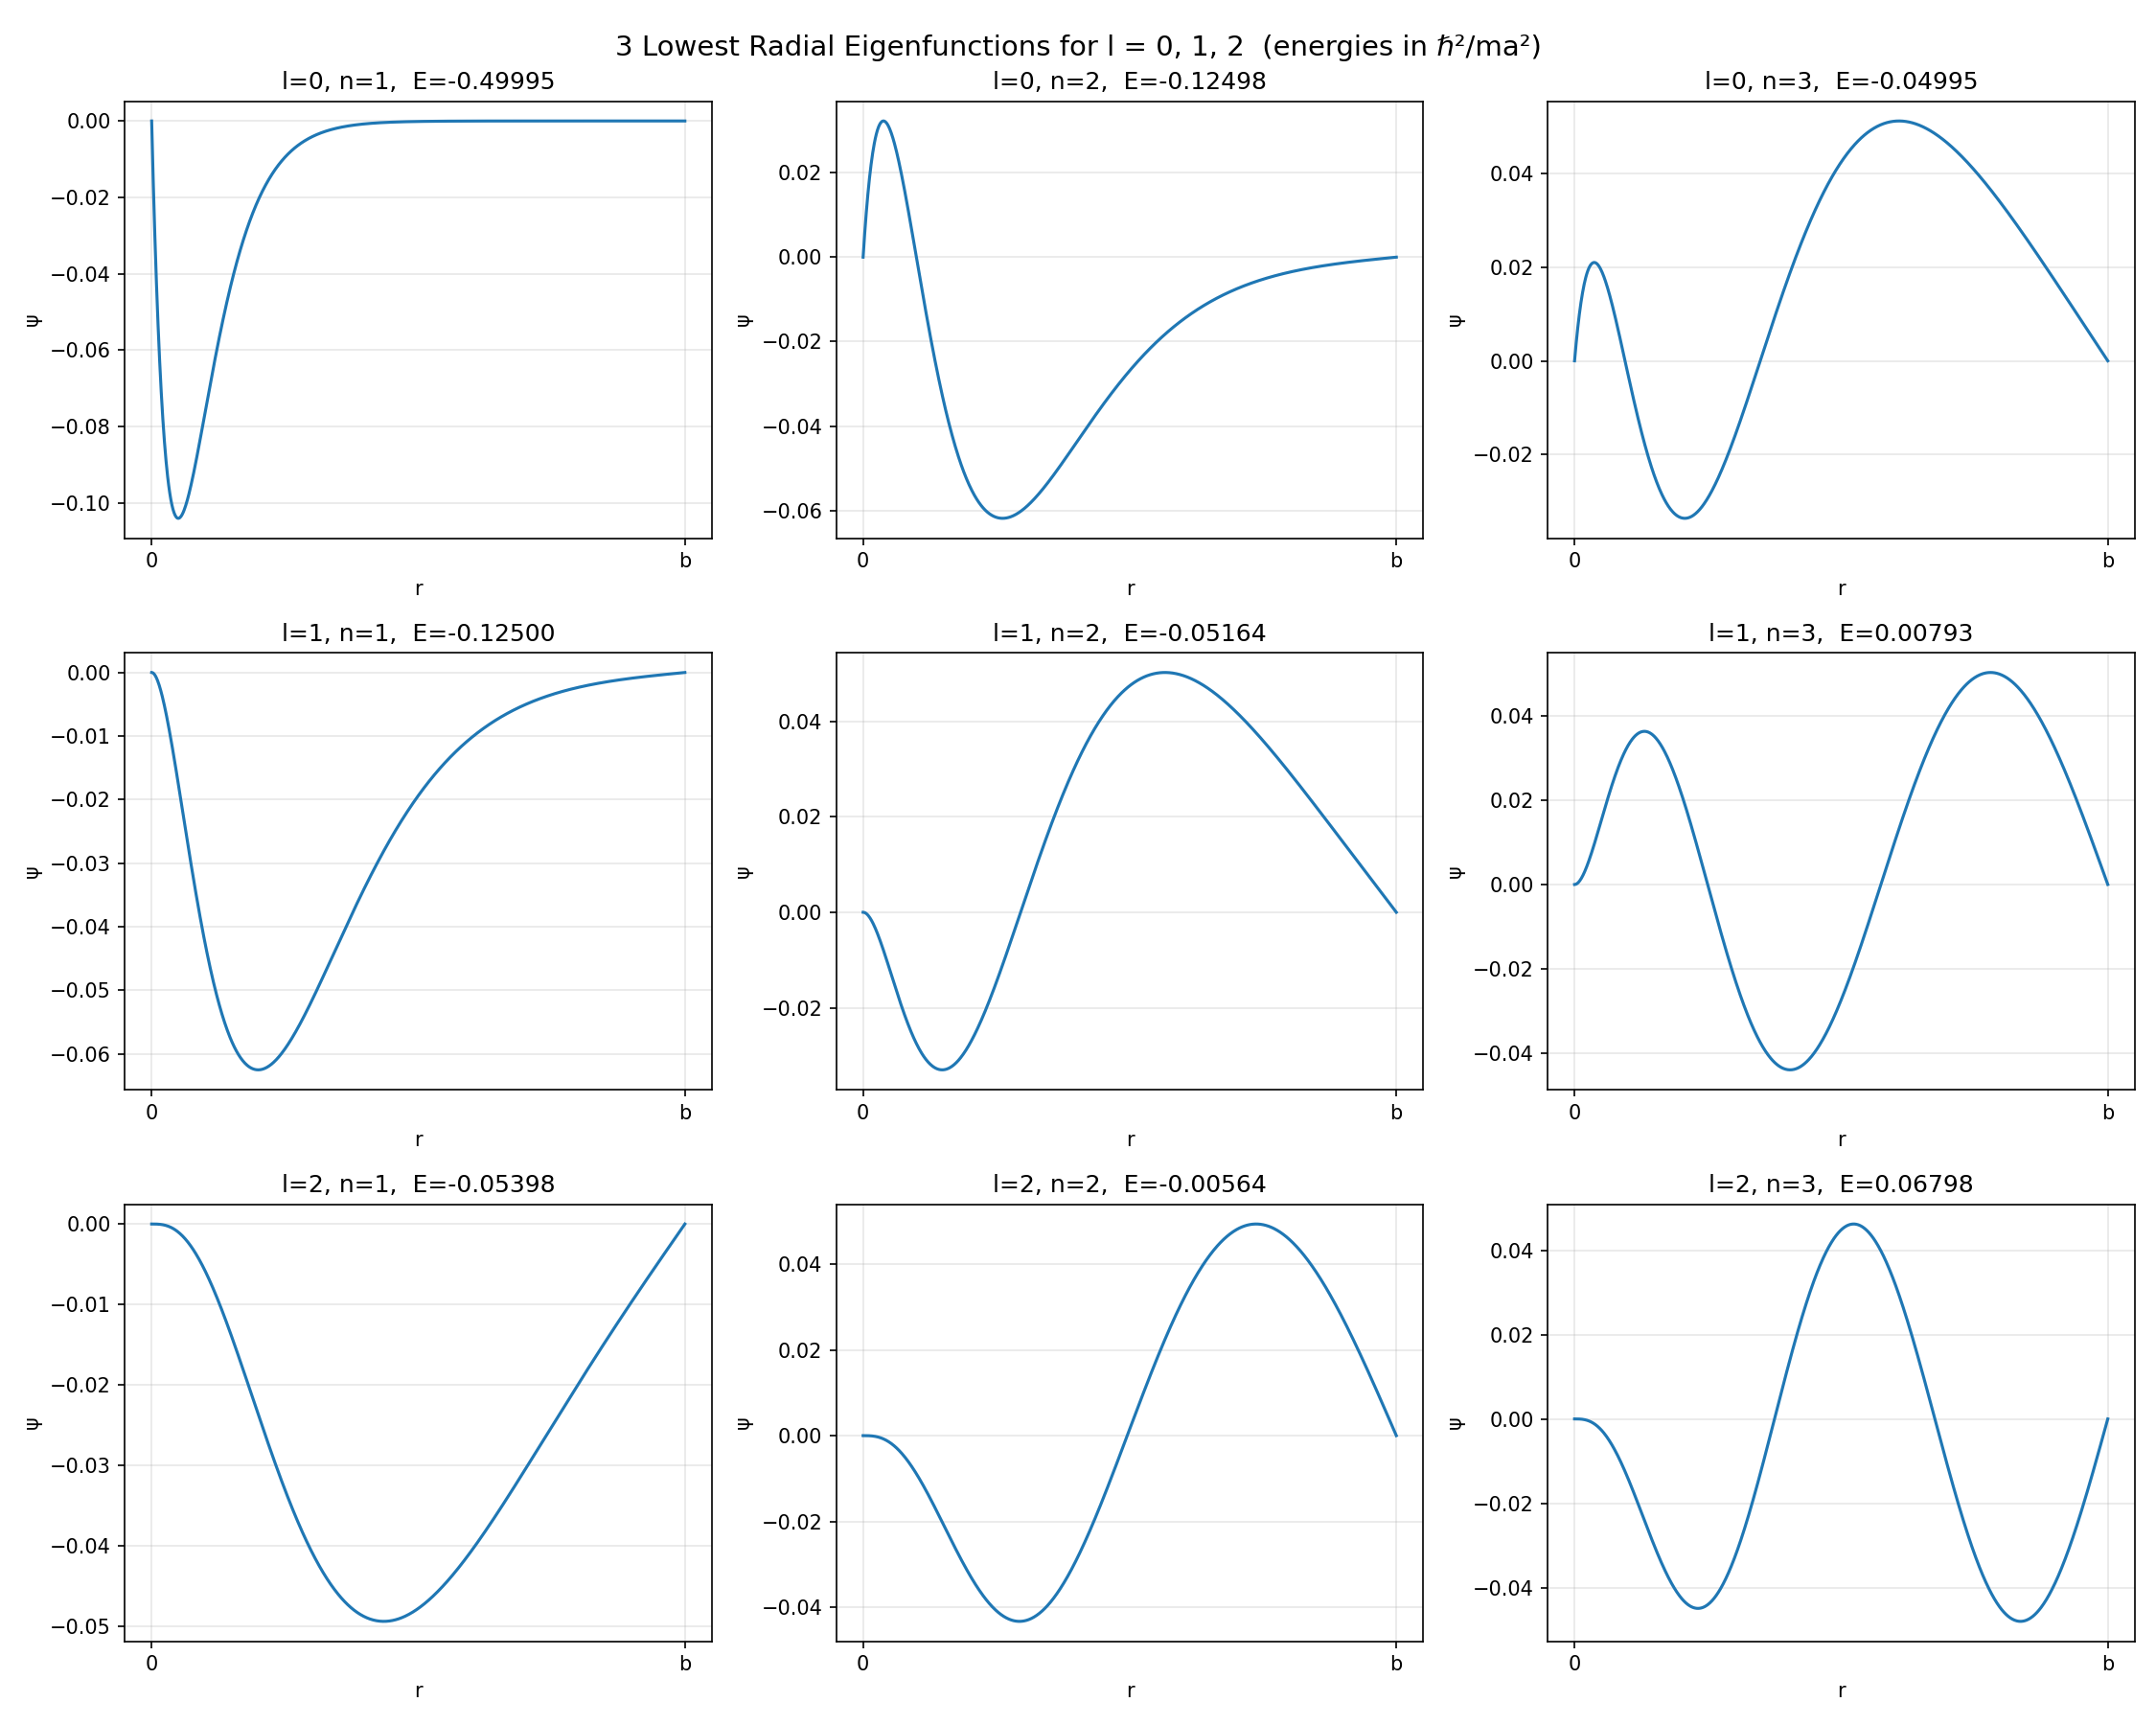
\includegraphics[valign=t,width=\textwidth]{fig/prob4.68_eigenfunctions.png}
     By eq 4.70, the lowest three energies in $\frac{\hbar^2}{ma^2}$ unit are $-0.5,\; -0.125, \;-0.0556.$
 \end{enumerate}
 \subsection*{Sol. 69}
 For $l=0,$ the lowest three $n$s are 
 $1.0000,$ $2.0000,$ $3.0000$.
 
 For $l=1,$ the lowest three $n$s are 
 $2.0000,$ $3.0000,$ $4.0000$.

 For $l=2,$ the lowest three $n$s are 
 $3.0000,$ $4.0000,$ $5.0000$.

 \subsection*{Sol. 70}
 \begin{enumerate}
     \item 
     All got spin up in the first experiment. If that particle is in the z direction group, it measured spin up for sure. If it is in the x direction group, since it is selected as spin up, the  measurement first time is spin up for sure.
     \item 
     Equation 4.155 gives 
     $$
     \chi_+^{(r)}
     =
     \begin{pmatrix}
         \cos\theta/2\\
         e^{i\phi}
         \sin\theta/2
     \end{pmatrix},\;
     \chi_-^{(r)}
     =
     \begin{pmatrix}
         e^{-i\phi}
         \sin\theta\\
         -\cos\theta/2
     \end{pmatrix}
     $$
     Note that, by choosing $\bm a$ as the z axis, the probability of measuring spin up along $\bm b$ for a spin up $\bm a$ particle is 
     \begin{align*}
         &\bigg|
         \begin{pmatrix}
         1 && 0
     \end{pmatrix}
         \begin{pmatrix}
             \cos\theta_{ab}/2\\
             e^{i\phi}
             \sin\theta_{ab}/2
         \end{pmatrix}
         \bigg|^2\\
         =&
         \cos^2\frac{\theta_{ab}}{2}
     \end{align*}
     We can get all four probabilities 
     $$
     P_{++}
     =
    \cos^2\frac{\theta_{bc}}{2} \cos^2\frac{\theta_{ab}}{2}
     $$
     $$
     P_{+-}
     =
    \sin^2\frac{\theta_{bc}}{2} \cos^2\frac{\theta_{ab}}{2}
     $$
     $$
     P_{-+}
     =
    \sin^2\frac{\theta_{bc}}{2} \sin^2\frac{\theta_{ab}}{2}
     $$
     $$
     P_{--}
     =
    \cos^2\frac{\theta_{bc}}{2} \sin^2\frac{\theta_{ab}}{2}
     $$
     \begin{align*}
         P_{\text{first up}|\text{second up}}
         =&\frac{\cos^2\frac{\theta_{bc}}{2} \cos^2\frac{\theta_{ab}}{2}}
         {\sin^2\frac{\theta_{bc}}{2} \sin^2\frac{\theta_{ab}}{2}+\cos^2\frac{\theta_{bc}}{2} \cos^2\frac{\theta_{ab}}{2}}\\
         =&(1+\tan^2\frac{\theta_{ab}}{2}\tan^2\frac{\theta_{bc}}{2})^{-1}.
     \end{align*}
     
 \end{enumerate}
 \subsection*{Sol. 71}
 \begin{enumerate}
     \item 
     $$
     \psi_{21-1}(r,\theta,\phi)
     =\frac{1}{2\sqrt{6}}a^{-3/2}\frac{r}{a}\exp(-\frac{r}{2a})\sqrt{\frac{3}{8\pi}}\sin\theta e^{-i\phi}
     $$
     $$
     \psi_{210}(r,\theta,\phi)
     =\frac{1}{2\sqrt{6}}a^{-3/2}\frac{r}{a}\exp(-\frac{r}{2a})\sqrt{\frac{3}{4\pi}}\cos\theta
     $$
     $$
     \psi_{211}(r,\theta,\phi)
     =-\frac{1}{2\sqrt{6}}a^{-3/2}\frac{r}{a}\exp(-\frac{r}{2a})\sqrt{\frac{3}{8\pi}}\sin\theta e^{i\phi}
     $$

     \begin{align*}
         \psi_{2p_x}(r,\theta,\phi)
         =\frac{1}{\sqrt{32\pi a^3}}\frac{r\sin\theta\cos\phi}{a}\exp(-\frac{r}{2a})
         =
         \frac{1}{\sqrt{2}}\psi_{21-1}(r,\theta,\phi)
         -\frac{1}{\sqrt{2}}\psi_{211}(r,\theta,\phi)
     \end{align*}
     \begin{align*}
         \psi_{2p_y}(r,\theta,\phi)
         =\frac{1}{\sqrt{32\pi a^3}}\frac{r\sin\theta\sin\phi}{a}\exp(-\frac{r}{2a})
         =
         \frac{i}{\sqrt{2}}\psi_{21-1}(r,\theta,\phi)
         +\frac{i}{\sqrt{2}}\psi_{211}(r,\theta,\phi)
     \end{align*}
     \begin{align*}
         \psi_{2p_z}(r,\theta,\phi)
         =\frac{1}{\sqrt{32\pi a^3}}\frac{r\cos\theta}{a}\exp(-\frac{r}{2a})
         =\psi_{210}(r,\theta,\phi)
     \end{align*}
     \item 
     \begin{align*}
         L_x\psi_{2p_x}
         =&
         -i\hbar(-\sin\phi\frac{\partial}{\partial\theta}-\cos\phi\cot\theta\frac{\partial}{\partial\phi})
         \frac{1}{\sqrt{32\pi a^3}}\frac{r\sin\theta\cos\phi}{a}\exp(-\frac{r}{2a})\\
         =&
         \frac{-i\hbar}{\sqrt{32\pi a^3}}\frac{r}{a}\exp(-\frac{r}{2a})
         (-\sin\phi\cos\theta\cos\phi + \cos\phi\cot\theta\sin\theta\sin\phi)\\
         =&0
     \end{align*}
     \begin{align*}
         L_y\psi_{2p_y}
         =&
         -i\hbar(\cos\phi\frac{\partial}{\partial\theta}-\sin\phi\cot\theta\frac{\partial}{\partial\phi})
         \frac{1}{\sqrt{32\pi a^3}}\frac{r\sin\theta\sin\phi}{a}\exp(-\frac{r}{2a})\\
         =&-i\hbar\frac{1}{\sqrt{32\pi a^3}}\frac{r}{a}\exp(-\frac{r}{2a})
         (\cos\phi\cos\theta\sin\phi-\sin\phi\cot\theta\sin\theta\cos\phi)\\
         =&0
     \end{align*}
     \begin{align*}
         L_z\psi_{2p_z}=&
         -i\hbar\frac{\partial}{\partial\phi}
         \frac{1}{\sqrt{32\pi a^3}}\frac{r\cos\theta}{a}\exp(-\frac{r}{2a})\\
         =&0
     \end{align*}
     \item 
     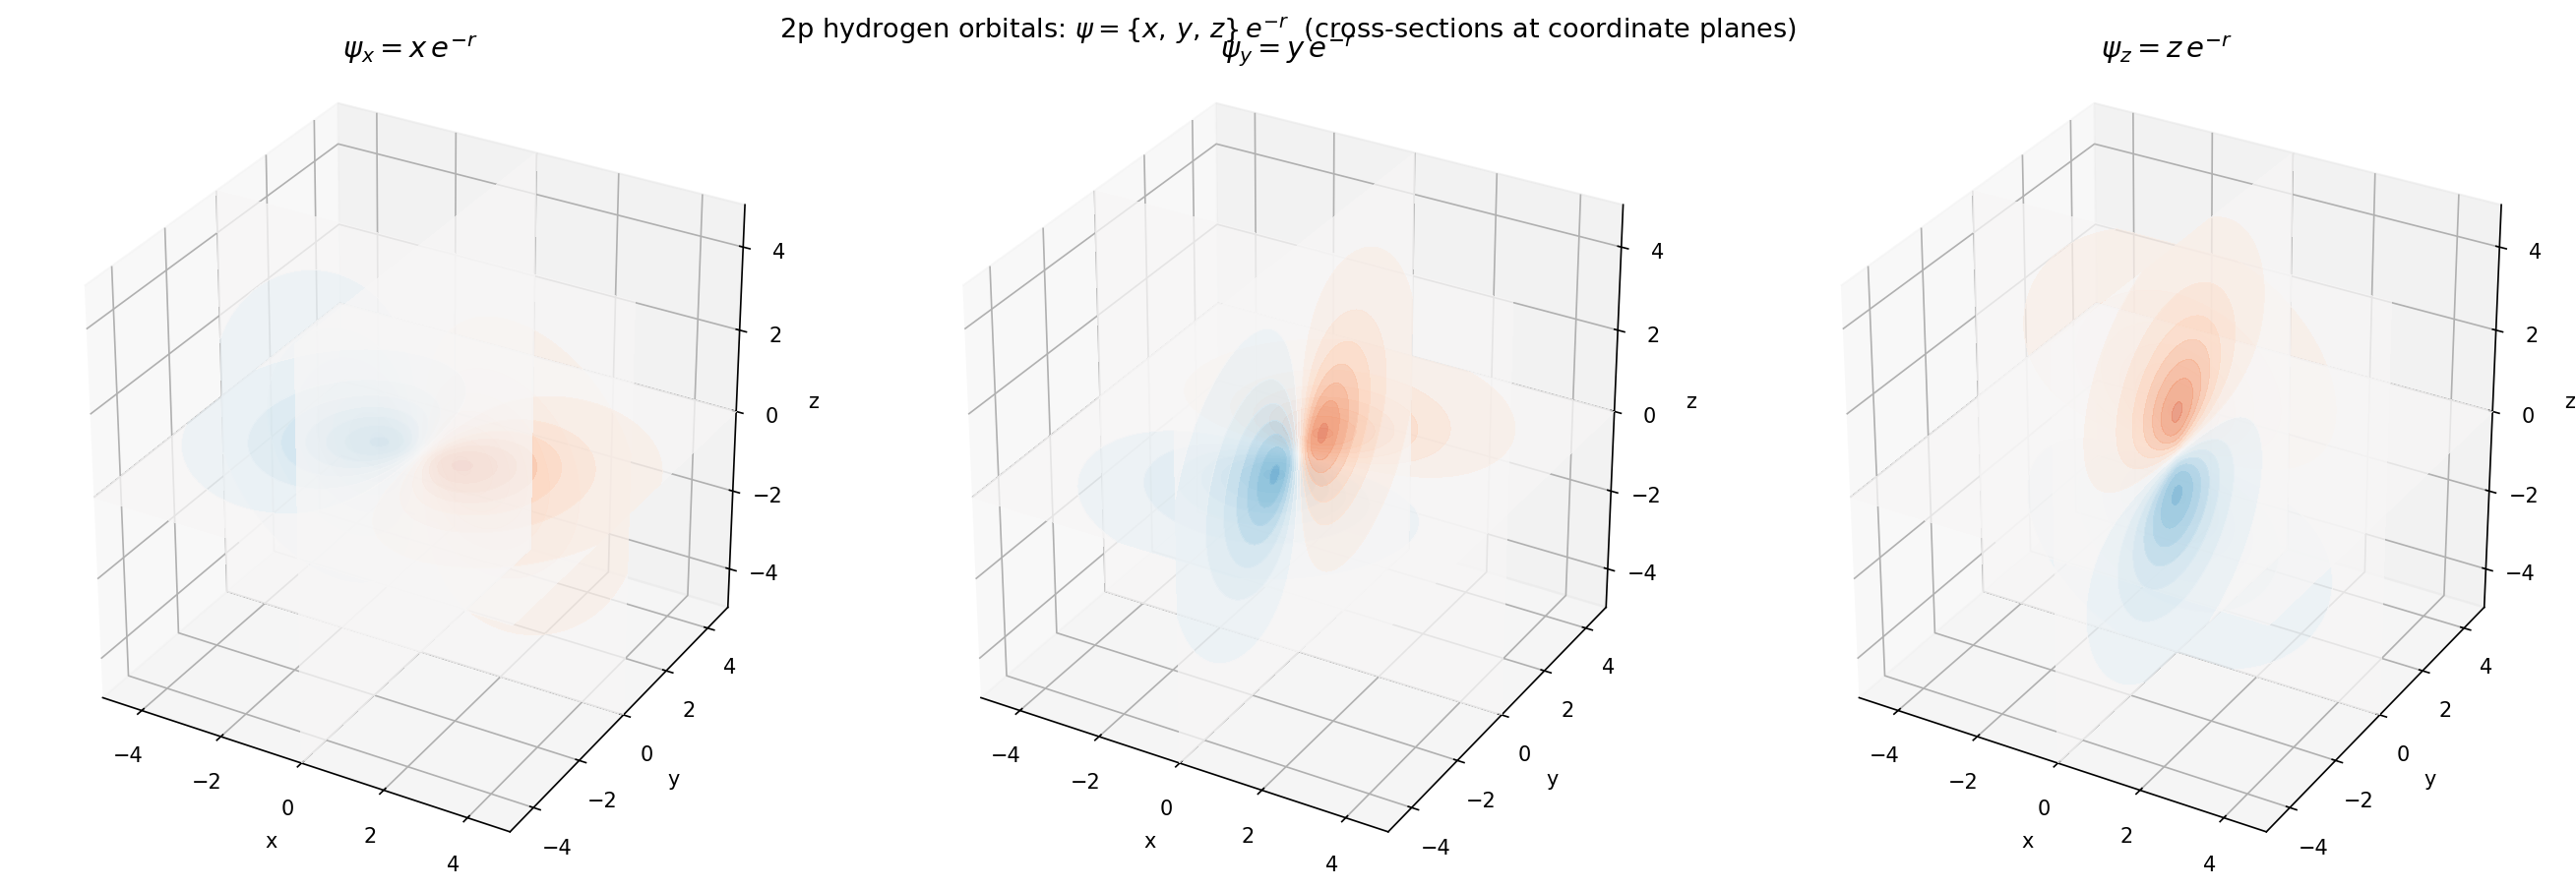
\includegraphics[valign=t,width=\textwidth]{fig/prob4.71_orbitals.png}
 \end{enumerate}
 \subsection*{Sol. 72}
 \begin{enumerate}
     \item 
     \begin{align*}
         \nabla\times\bm A =&
         \nabla\times(-\frac{1}{2}\bm r \times \bm B_0)\\
         = &
         -\frac{1}{2}\nabla\times
         ((yB_{0z}-zB_{0y})\hat i+
         (zB_{0x}-xB_{0y})\hat j +
         (xB_{0y}-yB_{0x})\hat k)\\
         =&
         -\frac{1}{2}
         ((-B_{0x}-B_{0x})\hat i +
         (-B_{0y}-B_{0y})\hat j +
         (-B_{0z}-B_{0z})\hat k)\\
         =&\bm B_0
     \end{align*}
     \item By equation 4.199 and equation 4.157
     \begin{align*}
         H =& \frac{1}{2m}
         (p^2+q^2\frac{1}{4}(\bm r\times \bm B_0)^2
         -i\hbar q(\bm r\times \bm B_0)\cdot\nabla)-\bm B_0\cdot(\gamma\bm S)+q\varphi
     \end{align*}
     \begin{align*}
         (\bm r\times \bm B_0)^2
         =r^2B_0^2-(\bm r\cdot \bm B_0)^2
     \end{align*}
     \begin{align*}
         -i\hbar q(\bm r\times \bm B_0)\cdot \nabla\psi
         =&i\hbar q\bm B_0\cdot (\bm r\times \nabla\psi)\\
         =&-q\bm B_0\cdot \bm L\psi,
     \end{align*}
     so 
     \begin{align*}
         H = 
         \frac{p^2}{2m}
         +q\varphi 
         -\bm B_0\cdot
         (\gamma_0\bm L+\gamma \bm S)
         +
         \frac{q^2}{8m}
         (r^2B_0^2-(\bm r\cdot \bm B_0)^2).
     \end{align*}
     
 \end{enumerate}
 \subsection*{Sol. 73}
 $$
 \bm B = -\alpha x\hat i + (B_0+\alpha z)\hat k 
 $$
 \begin{align*}
     \frac{d^2}{dt^2}
     \langle z\rangle
     =&
     \frac{i}{\hbar}
     \frac{d}{dt}
     \langle[H,z]\rangle\\
     =&\frac{i}{\hbar}
     \frac{i}{\hbar}
     \langle[H,[H,z]]\rangle\\
     =&-\frac{1}{\hbar^2}
     \langle[\frac{p^2}{2m}-\gamma\bm B\cdot \bm S, -2i\hbar p_z]\rangle\\
     =&-\frac{1}{\hbar^2}
     \langle-\gamma \alpha z S_z, \frac{-2i\hbar}{2m} p_z\rangle\\
     =&\frac{1}{m}\gamma\alpha\langle S_z\rangle.
 \end{align*}

 \subsection*{Sol. 74}
 \begin{enumerate}
     \item 
     \begin{align*}
         (\frac{p^2}{2m}-\gamma\bm B\cdot\bm S)
         (\Psi_+\chi_++\Psi_-\chi_-)
         =i\hbar\frac{\partial}{\partial t}
         (\Psi_+\chi_++\Psi_-\chi_-)
     \end{align*}
     \begin{align*}
         &(-\frac{\hbar^2}{2m}\nabla^2
         -\gamma(-\alpha xS_x+(B_0+\alpha z)S_z))
         (\Psi_+\chi_++\Psi_-\chi_-)\\
         =&
         -\frac{\hbar^2}{2m}\nabla^2\Psi_+\chi_+
         -\frac{\hbar^2}{2m}\nabla^2\Psi_-\chi_-
         +\gamma\alpha x\Psi_+\frac{\hbar}{2}\chi_-\\
         &+\gamma\alpha x\Psi_-\frac{\hbar}{2}\chi_+
         -\gamma(B_0+\alpha z)\Psi_+\frac{\hbar}{2}\chi_+
         +\gamma(B_0+\alpha z)\Psi_-\frac{\hbar}{2}\chi_-
     \end{align*}
     We therefore have two coupled equations
     \begin{align*}
         -\frac{\hbar^2}{2m}\nabla^2\Psi_+
         +\frac{\hbar}{2}\gamma\alpha x\Psi_- 
         -\frac{\hbar}{2}\gamma (B_0+\alpha z)\Psi_+ = 
         i\hbar \frac{\partial}{\partial t}\Psi_+
     \end{align*}
     \begin{align*}
         -\frac{\hbar^2}{2m}\nabla^2\Psi_-
         +\frac{\hbar}{2}\gamma\alpha x\Psi_+ 
         +\frac{\hbar}{2}\gamma (B_0+\alpha z)\Psi_- = 
         i\hbar \frac{\partial}{\partial t}\Psi_-
     \end{align*}
     \item 
     \begin{align*}
         -\frac{\hbar^2}{2m}\nabla^2
         e^{i\gamma B_0t/2}\tilde\Psi_+
         +\frac{\hbar}{2}\gamma\alpha x
         e^{-i\gamma B_0t/2}\tilde\Psi_-
         -\frac{\hbar}{2}\gamma (B_0+\alpha z)
         e^{i\gamma B_0t/2}\tilde\Psi_+= 
         i\hbar \frac{\partial}{\partial t}
         e^{i\gamma B_0t/2}\tilde\Psi_+
     \end{align*}
     \begin{align*}
         -\frac{\hbar^2}{2m}\nabla^2
         \tilde\Psi_+
         +\frac{\hbar}{2}\gamma\alpha x
         e^{-i\gamma B_0t}\tilde\Psi_-
         -\frac{\hbar}{2}\gamma \alpha z
         \tilde\Psi_+= 
         i\hbar \frac{\partial}{\partial t}
         \tilde\Psi_+
     \end{align*}
     \begin{align*}
         -\frac{\hbar^2}{2m}\nabla^2
         e^{-i\gamma B_0t/2}\tilde\Psi_-
         +\frac{\hbar}{2}\gamma\alpha x
         e^{i\gamma B_0t/2}\tilde\Psi_+ 
         +\frac{\hbar}{2}\gamma (B_0+\alpha z)
         e^{-i\gamma B_0t/2}\tilde\Psi_- = 
         i\hbar \frac{\partial}{\partial t}
         e^{-i\gamma B_0t/2}\tilde\Psi_-
     \end{align*}
     \begin{align*}
         -\frac{\hbar^2}{2m}\nabla^2
         \tilde\Psi_-
         +\frac{\hbar}{2}\gamma\alpha x
         e^{i\gamma B_0t}\tilde\Psi_+ 
         +\frac{\hbar}{2}\gamma \alpha z
         \tilde\Psi_- = 
         i\hbar \frac{\partial}{\partial t}
         \tilde\Psi_-
     \end{align*}
     \item 
     \begin{align*}
         -\frac{\hbar^2}{2m}
         \nabla^2\tilde\Psi_{\pm}
         \mp\frac{\hbar}{2}\gamma\alpha z\tilde\Psi_{\pm}
         =i\hbar\frac{\partial}{\partial t}\tilde\Psi_{\pm}
     \end{align*}

        By Ehrenfest's Theorem, the expectation value of the z component of $\tilde\Psi_+$ goes up, and the expectation value of the z component of $\tilde\Psi_-$ goes down, splitting both spatial wave functions apart. Once it hits the screen,
        the spin state collapses, and the difference in the z component of both states makes the two stripes.
 \end{enumerate}

 \subsection*{Sol. 75}
 \begin{align*}
     H\Psi(\phi,t)
    =& \frac{1}{2m}
    \left[
    -\frac{\hbar^2}{b^2}\frac{d^2}{d\phi^2}
    +\left(
    \frac{q\Phi}{2\pi b}
    \right)^2
    +
    i\frac{\hbar q\Phi}{\pi b^2}
    \frac{d}{d\phi}
    \right]
    \frac{1}{\sqrt{2\pi}}
    e^{in\phi}
    e^{-if(t)}\\
    =&\frac{1}{2m}
    \left[
    \frac{\hbar^2}{b^2}n^2
    +\left(
    \frac{q\Phi}{2\pi b}
    \right)^2
    -
    \frac{\hbar q\Phi n}{\pi b^2}
    \right]
    \frac{1}{\sqrt{2\pi}}
    e^{in\phi}
    e^{-if(t)}\\
    =&\frac{1}{\sqrt{2\pi}}
     e^{in\phi}
     e^{-if(t)}
     \frac{\hbar^2}{2mb^2}
     \left(
    n- \frac{q\Phi}{2\pi\hbar}
     \right)^2
 \end{align*}
 \begin{align*}
     i\hbar\frac{\partial}{\partial t}
     \frac{1}{\sqrt{2\pi}}
     e^{in\phi}
     e^{-if(t)}
     =& 
     i\hbar
     \frac{1}{\sqrt{2\pi}}
     e^{in\phi}
     e^{-if(t)}
     (-if'(t))\\
     =&
     \frac{1}{\sqrt{2\pi}}
     e^{in\phi}
     e^{-if(t)}
     \frac{\hbar^2}{2mb^2}
     \left(
    n- \frac{q\Phi}{2\pi\hbar}
     \right)^2
 \end{align*}

 \subsection*{Sol. 76}
 \begin{enumerate}
     \item 
     \begin{align*}
        \mathcal{E}
         =&-\frac{d\Phi}{dt}
         =2\pi Fb
     \end{align*}
     
     $$
     W = \int qF b\omega dt
     =-\int \frac{q\omega}{2\pi} d\Phi
     $$
     $$
     \frac{dW}{d\Phi}
     =-\frac{q\omega}{2\pi}.
     $$
     \item 
     \begin{align*}
         \bm r\times (\bm p - q\bm A)
         \frac{1}{\sqrt{2\pi}}
         \exp\left(
         in\phi
         \right)
         =&
         \bm r\times 
         (\frac{1}{\sqrt{2\pi}}\frac{1}{b}
         \hbar n
         \exp\left(
         in\phi
         \right)\hat\phi -
         \frac{1}{\sqrt{2\pi}}
         \frac{q\Phi}{2\pi b}
         \exp\left(
         in\phi
         \right)\hat\phi
         )
     \end{align*}
     The z component is 
     \begin{align*}
         \frac{1}{\sqrt{2\pi}}
         \hbar n
         \exp\left(
         in\phi
         \right) -
         \frac{1}{\sqrt{2\pi}}
         \frac{q\Phi}{2\pi}
         \exp\left(
         i n\phi
         \right),
     \end{align*}
     so the $z$ component of the mechanical angular momentum is 
     $\hbar n-\frac{q\Phi}{2\pi}.$
     \item 
     $$
     L = mb^2\omega,
     $$
     so
     \begin{align*}
         \frac{dE_n}{d\Phi}
         =&
         \frac{\hbar^2}{2mb^2}
         2\left(
         n-\frac{q\Phi}{2\pi\hbar}
         \right)
         (-\frac{q}{2\pi\hbar})\\
         =&
         -
         \frac{\hbar^2}{2mb^2}
         2\frac{mb^2\omega}{\hbar}
         \frac{q}{2\pi\hbar}\\
         =&-
         \frac{q\omega}{2\pi}
         =\frac{dW}{d\Phi}
     \end{align*}
 \end{enumerate}

\section{Identical Particles}
\subsection*{Sol. 1}
\begin{enumerate}
    \item 
    \begin{align*}
        \bm R + \frac{\mu}{m_1}\bm r= 
        \frac{m_1\bm r_1+m_2\bm r_2}{m_1+m_2}
        +
        \frac{m_2}{m_1+m_2}
        (\bm r_1-\bm r_2)
        =\bm r_1
    \end{align*}
    \begin{align*}
        \bm R - \frac{\mu}{m_1}\bm r= 
        \frac{m_1\bm r_1+m_2\bm r_2}{m_1+m_2}
        -
        \frac{m_2}{m_1+m_2}
        (\bm r_1-\bm r_2)
        =\bm r_2
    \end{align*}
    By the chain rule
    \begin{align*}
        \begin{pmatrix}
        \nabla_R(g\circ f) && \nabla_r(g\circ f)
        \end{pmatrix}
        =&
        \begin{pmatrix}
        \nabla_1 g && \nabla_2g
        \end{pmatrix}
        \begin{pmatrix}
            \frac{\partial f_1}{\partial R} & \frac{\partial f_1}{\partial r}\\
            \frac{\partial f_2}{\partial R} & \frac{\partial f_2}{\partial r}
        \end{pmatrix}\\
        =&
        \begin{pmatrix}
        \nabla_1 g && \nabla_2g
        \end{pmatrix}
        \begin{pmatrix}
            1 & \frac{\mu}{m_1}\\
            1 & -\frac{\mu}{m_2}
        \end{pmatrix},
    \end{align*}
    $$
    \begin{pmatrix}
            1 & \frac{\mu}{m_1}\\
            1 & -\frac{\mu}{m_2}
        \end{pmatrix}^{-1}
        =\begin{pmatrix}
            \frac{\mu}{m_2} & \frac{\mu}{m_1}\\
            1 & -1
        \end{pmatrix}
    $$
    so 
    $$
    \nabla_1 = \frac{\mu}{m_2}\nabla_R +\nabla_r
    $$
    $$
    \nabla_2 = \frac{\mu}{m_1}\nabla_R -\nabla_r.
    $$
    \item 

    \begin{align*}
        -\frac{\hbar^2}{2m_1}
        (\frac{\mu}{m_2}\nabla_R +\nabla_r)^2\psi
        -\frac{\hbar^2}{2m_2}
        (\frac{\mu}{m_1}\nabla_R -\nabla_r)^2\psi
        +V(r)\psi = E\psi
    \end{align*}
    \begin{align*}
        (-\frac{\hbar^2\mu^2}{2m_1m_2^2}
        -\frac{\hbar^2\mu^2}{2m_2m_1^2})
        \nabla^2_R
        \psi 
        +
        (-\frac{\hbar^2}{2m_1}
        -\frac{\hbar^2}{2m_2})
        \nabla_r^2 \psi 
        +V(r)\psi = E\psi.
    \end{align*}
    \begin{align*}
        -\frac{\hbar^2}{2(m_1+m_2)}
        \nabla^2_R\psi 
        -
        \frac{\hbar^2}{2\mu}
        \nabla_r^2\psi + V(r)\psi = E\psi.
    \end{align*}
    \item 
    $$
    -\frac{\hbar^2}{2(m_1+m_2)}
        \nabla^2_R\psi_R(R) = E_R\psi_R(R)
    $$
    $$
    -\frac{\hbar^2}{2\mu}
        \nabla_r^2\psi_r(r) + V(r)\psi_r(r) = E_r\psi_r(r).
    $$
\end{enumerate}

\subsection*{Sol. 2}
\begin{enumerate}
    \item 
    $m_e=9.1093837\times 10^{-31}kg,$
$\mu = \frac{9.1093837\times 10^{-31}\times 1.67262192\times 10^{-27}}
{9.1093837\times 10^{-31}+1.67262192\times 10^{-27}}
\approx 9.10442527501427\times 10^{-31}kg
$

$$
\frac{E}{E_1}-1 = 
\frac{\mu}{m_e} - 1
\approx -0.05\%
$$
\item 
The modified Rydberg constant is 
$1.0964\times10^7m^{-1},$ 
$$
\frac{1}{\lambda}=
1.0964\times10^7\times(\frac{1}{4}-\frac{1}{9})
\Rightarrow \lambda\approx 6.5669\times 10^{-7}m
$$

For the deuterium, $\mu\approx 9.1069\times10^{-31}kg,$ so the 
modified Rydberg constant is  $1.0967\times10^7m^{-1},$
$$
\frac{1}{\lambda}=
1.0967\times10^7\times(\frac{1}{4}-\frac{1}{9})
\Rightarrow \lambda\approx 6.56514\times 10^{-7}m
$$

\item 
The reduced mass is only half the electron mass, so 
the binding energy for the positronium is $-6.8eV.$
\item The reduced mass is now $1.6929\times 10^{-28}kg,$ so 
the Rydberg constant is $2038689171,$ thus 
$$
\frac{1}{\lambda} = 2038689171(1-\frac{1}{4})
\Rightarrow \lambda =  6.54\times 10^{-10}m
$$


\end{enumerate}


\subsection*{Sol. 3}
The ratio of the energies for the two isotopes is 
$$
\frac{\omega_1}{\omega_2}
=\sqrt{\frac{\mu_2}{\mu_1}}
=\sqrt{\frac{m_{37}}{m_{35}}\frac{m_H+m_{35}}{m_H+m_{37}}}
=\sqrt{\frac{17+20}{17+18}\frac{17+18+1}{17+20+1}}
=1.000751,
$$
so the difference between two vibrational spectrum is 
$7.51\times 10^{-4}\nu.$

\subsection*{Sol. 4}
\begin{enumerate}
    \item 
    \begin{align*}
        &\int A^2
        (\psi_a(\bm r_1)\psi_b(\bm r_2)
        +\psi_a(\bm r_2)\psi_b(\bm r_1))^2
        d^3\bm r_1
        d^3\bm r_2\\
        =&
        A^2\int
        \psi_a(\bm r_1)^2
        \psi_b(\bm r_2)^2
        d^3\bm r_1
        d^3\bm r_2
        +
        A^2\int
        \psi_a(\bm r_2)^2
        \psi_b(\bm r_1)^2
        d^3\bm r_1
        d^3\bm r_2\\
        &+
        2A^2\int
        \psi_a(\bm r_1)
        \psi_b(\bm r_2)
        \psi_a(\bm r_2)
        \psi_b(\bm r_1)
        d^3\bm r_1
        d^3\bm r_2\\
        =&
        A^2+A^2\Rightarrow A=\frac{1}{\sqrt{2}}.
    \end{align*}
    \item 
    \begin{align*}
        &\int 4A^2
        \psi_a^2(\bm r_1)
        \psi_a^2(\bm r_2)
        d^3\bm r_1
        d^3\bm r_2
        \Rightarrow A=\frac{1}{2}.
    \end{align*}
\end{enumerate}

\subsection*{Sol. 5}
\begin{enumerate}
    \item 
    $$
    H = -\frac{\hbar^2}{2m_1}\nabla_1^2
    -\frac{\hbar^2}{2m_2}\nabla_2^2
    +V(x_1)+V(x_2),
    $$
    where $V(x)=0$ if $0<x<a,$ and $\infty$ otherwise.

    \begin{align*}
        &(-\frac{\hbar^2}{2m}\nabla_1^2
    -\frac{\hbar^2}{2m}\nabla_2^2)
        \left[
        \sin(\frac{\pi x_1}{a})
        \sin(\frac{2\pi x_2}{a})
        -
        \sin(\frac{2\pi x_1}{a})
        \sin(\frac{\pi x_2}{a})
        \right]\\
        =&
        \frac{\hbar^2}{2m}
        \frac{\pi^2}{a^2}\sin(\frac{\pi x_1}{a})
        \sin(\frac{2\pi x_2}{a})
        -
        \frac{\hbar^2}{2m}
        \frac{4\pi^2}{a^2}
        \sin(\frac{2\pi x_1}{a})
        \sin(\frac{\pi x_2}{a})\\
        &+\frac{\hbar^2}{2m}
        \frac{4\pi^2}{a^2}\sin(\frac{\pi x_1}{a})
        \sin(\frac{2\pi x_2}{a})
        -\frac{\hbar^2}{2m}
        \frac{\pi^2}{a^2}
        \sin(\frac{2\pi x_1}{a})
        \sin(\frac{\pi x_2}{a})\\
        =&
        \frac{5\hbar^2\pi^2}{2ma^2}
        \left[
        \sin(\frac{\pi x_1}{a})
        \sin(\frac{2\pi x_2}{a})
        -
        \sin(\frac{2\pi x_1}{a})
        \sin(\frac{\pi x_2}{a})
        \right]
    \end{align*}
    \item 
    The second excited state for the distinguishable particles is nondegenerate
    $$
    \psi_{22}=
    \frac{2}{a}\sin(\frac{2\pi x_1}{a})
    \sin(\frac{2\pi x_2}{a}),\; 
    E_{22}=8K,
    $$
    and the third excited state is doubly degenerate
    $$
    \psi_{13}=
    \frac{2}{a}\sin(\frac{\pi x_1}{a})
    \sin(\frac{3\pi x_2}{a}),\; 
    E_{13}=10K
    $$
    $$
    \psi_{31}=
    \frac{2}{a}\sin(\frac{3\pi x_1}{a})
    \sin(\frac{1\pi x_2}{a}).\; 
    E_{31}=10K.
    $$
    
    The second excited state for bosons is just like the distinguishable particles. The third excited state is 
    $$
    \frac{\sqrt{2}}{a}
    \left[
    \sin(\frac{\pi x_1}{a})
    \sin(\frac{3\pi x_2}{a})+
    \sin(\frac{3\pi x_1}{a})
    \sin(\frac{\pi x_2}{a})
    \right], \; 
    E = 10K.
    $$
    
    The first and second excited states for fermions are 
    $$
    \frac{\sqrt{2}}{a}
    \left[
    \sin(\frac{\pi x_1}{a})
    \sin(\frac{3\pi x_2}{a})-
    \sin(\frac{3\pi x_1}{a})
    \sin(\frac{\pi x_2}{a})
    \right],\;
    E = 10K
    $$
    and
    $$
    \frac{\sqrt{2}}{a}
    \left[
    \sin(\frac{2\pi x_1}{a})
    \sin(\frac{3\pi x_2}{a})-
    \sin(\frac{3\pi x_1}{a})
    \sin(\frac{2\pi x_2}{a})
    \right]
    , \; 
    E = 13K.
    $$
\end{enumerate}
\subsection*{Sol. 6}
Distinguishable:
   \begin{align*}
        \langle x^2\rangle_n
    +\langle x^2\rangle_l
    -2
    \langle x\rangle_n
    \langle x\rangle_l
    =&
    a^2\left(\frac{1}{3}-\frac{1}{2\pi^2n^2}    \right)
    +
    a^2\left(\frac{1}{3}-\frac{1}{2\pi^2l^2}    \right)
    -2\frac{a}{2}\frac{a}{2}\\
    =&
    a^2\left(\frac{1}{6}-\frac{1}{2\pi^2}
    \left(\frac{1}{n^2}+\frac{1}{l^2}\right)\right)
   \end{align*}
   \begin{align*}
       \langle x\rangle_{nl}
       =&\frac{2}{a}\int_0^ax\sin(\frac{n\pi}{a}x)\sin(\frac{l\pi}{a}x)dx\\
       =&\frac{1}{a}
       \int_0^a
       x\left[
       \cos(\frac{(n-l)\pi x}{a})
       -
       \cos(\frac{(n+l)\pi x}{a})
       \right]
       dx\\
       =&
       \frac{a}{(n-l)^2\pi^2}
       (\cos((n-l)\pi )-1)
       -\frac{a}{(n+l)^2\pi^2}
       (\cos((n+l)\pi )-1)
   \end{align*}
   If $n+l\equiv0\mod 2,$
   $$
   \langle x\rangle_{nl}=0,
   $$
    if $n+l\equiv0\mod 2,$
   $$
   \langle x\rangle_{nl}=
   \frac{-2a}{(n-l)^2\pi^2}-\frac{-2a}{(n+l)^2\pi^2}
   =\frac{-8anl}{(n+l)^2(n-l)^2\pi^2}.
   $$
   Bosons
   $$
   \langle(x_1-x_2)^2\rangle
   =a^2\left(\frac{1}{6}-\frac{1}{2\pi^2}
    \left(\frac{1}{n^2}+\frac{1}{l^2}\right)\right)
    -
    \left(\frac{8anl}{(n+l)^2(n-l)^2\pi^2}\right)^2
   $$
   Fermions
   $$
   \langle(x_1-x_2)^2\rangle
   =a^2\left(\frac{1}{6}-\frac{1}{2\pi^2}
    \left(\frac{1}{n^2}+\frac{1}{l^2}\right)\right)
    +
    \left(\frac{8anl}{(n+l)^2(n-l)^2\pi^2}\right)^2
   $$
   The last term is present only when $n,l$ have the same parity.
   
   
   \subsection*{Sol. 7}
   \begin{enumerate}
       \item 
       Distinguishable:
        $$
        \psi(x_1,x_2)=
        \left(
        \frac{m\omega}{\pi\hbar}
        \right)^{1/2}
        \sqrt{\frac{2m\omega}{\hbar}}
        x_2
        e^{-\frac{m\omega}{2\hbar}x_1^2}
        e^{-\frac{m\omega}{2\hbar}x_2^2}
        $$
    Bosons:
    $$
        \psi(x_1,x_2)=
        \frac{1}{\sqrt{2}}
        \left(
        \frac{m\omega}{\pi\hbar}
        \right)^{1/2}
        \sqrt{\frac{2m\omega}{\hbar}}
        \left[
        x_2
        e^{-\frac{m\omega}{2\hbar}x_1^2}
        e^{-\frac{m\omega}{2\hbar}x_2^2}
        +
        x_1
        e^{-\frac{m\omega}{2\hbar}x_1^2}
        e^{-\frac{m\omega}{2\hbar}x_2^2}
        \right]
        $$
    Fermions:
    $$
        \psi(x_1,x_2)=
        \frac{1}{\sqrt{2}}
        \left(
        \frac{m\omega}{\pi\hbar}
        \right)^{1/2}
        \sqrt{\frac{2m\omega}{\hbar}}
        \left[
        x_2
        e^{-\frac{m\omega}{2\hbar}x_1^2}
        e^{-\frac{m\omega}{2\hbar}x_2^2}
        -
        x_1
        e^{-\frac{m\omega}{2\hbar}x_1^2}
        e^{-\frac{m\omega}{2\hbar}x_2^2}
        \right]
        $$
        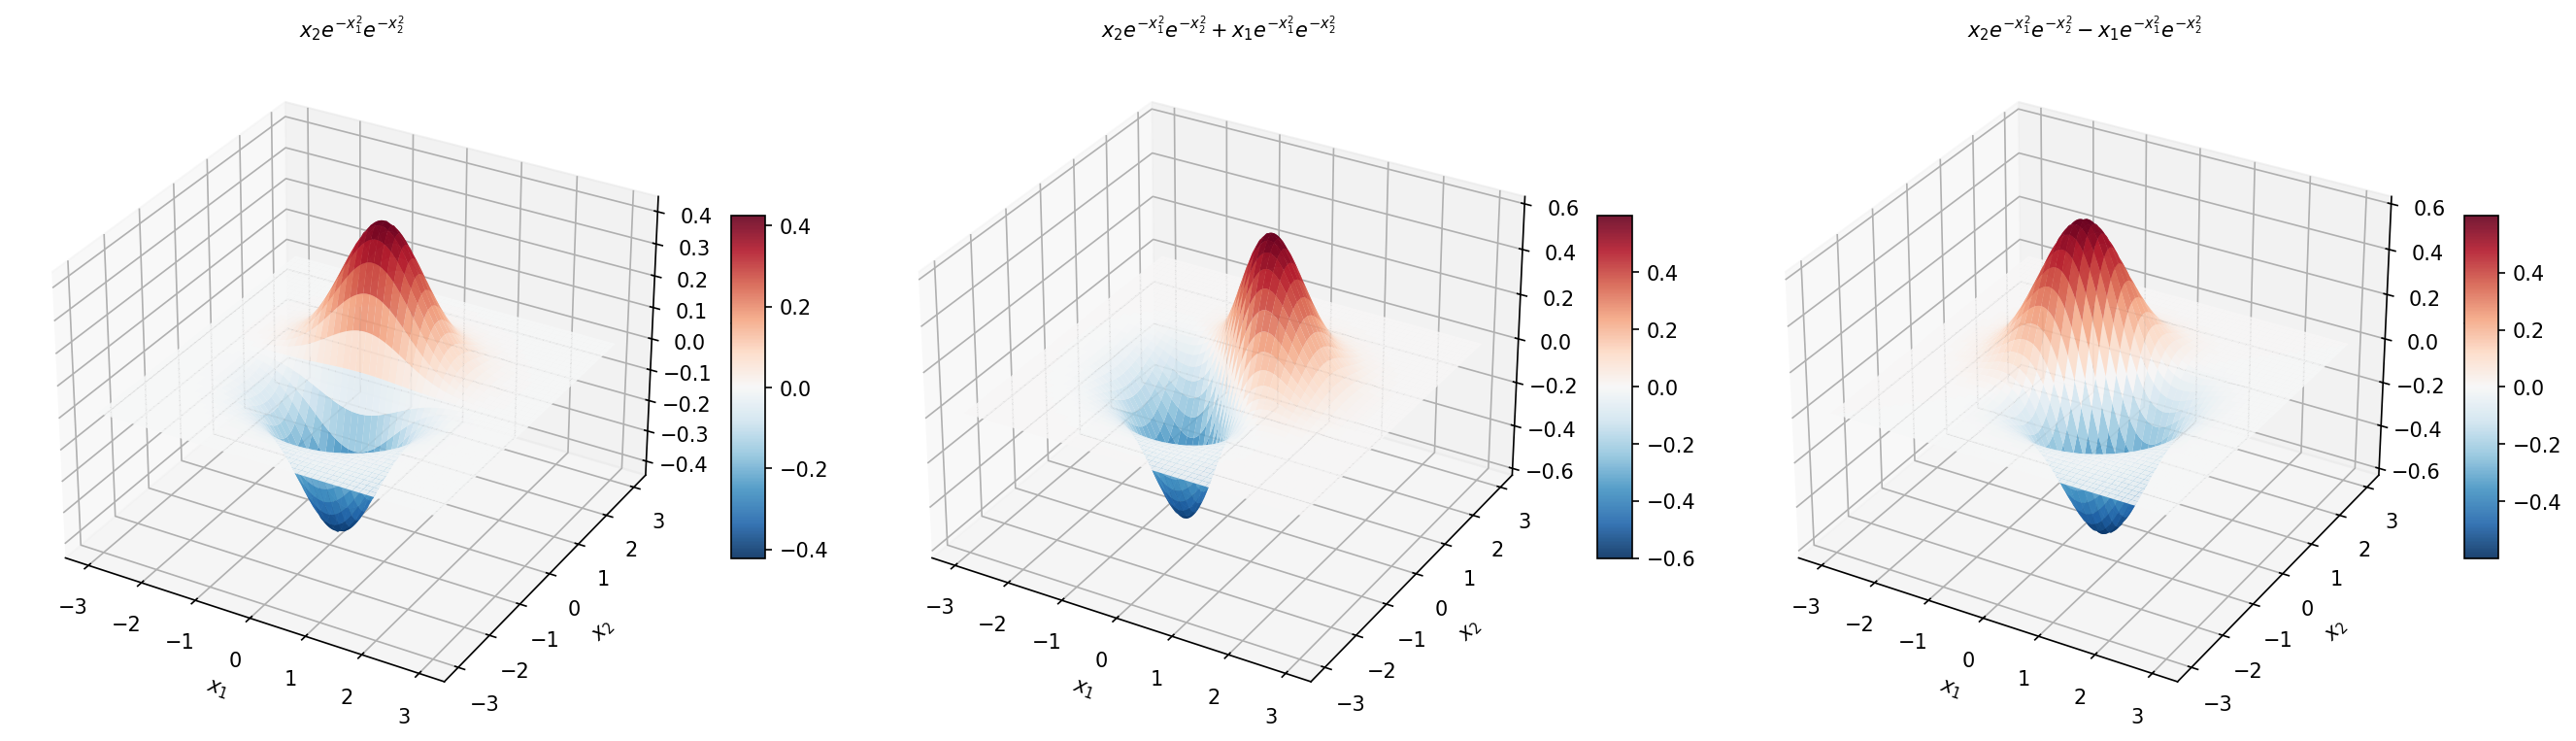
\includegraphics[width=0.8\textwidth,valign=t]{fig/prob5.7_surfaces.png}
        \item 
        $$
        \langle x^2\rangle_0 = \frac{\hbar}{2m\omega}
        $$
        $$
        \langle x^2\rangle_1 = \frac{3\hbar}{2m\omega}
        $$
        \begin{align*}
            \langle x\rangle_{01}=
            &\left(
        \frac{m\omega}{\pi\hbar}
        \right)^{1/2}
        \sqrt{\frac{2m\omega}{\hbar}}
            \int_{-\infty}^\infty
            x^2
        e^{-\frac{m\omega}{\hbar}x^2}
        dx
        \\
        =&
        \left(
        \frac{m\omega}{\pi\hbar}
        \right)^{1/2}
        \sqrt{\frac{2m\omega}{\hbar}}
        \frac{1}{2}
        \sqrt{\frac{\pi}{(\frac{m\omega}{\hbar})^3}}\\
        =&\sqrt{\frac{\hbar}{2m\omega}}
        \end{align*}
        Distinguishable 
        $$
        \langle(x_1-x_2)^2\rangle
        =\frac{2\hbar}{m\omega}
        $$
        Bosons 
        $$
        \langle(x_1-x_2)^2\rangle
        =\frac{\hbar}{m\omega}
        $$
        Fermions 
        $$
        \langle(x_1-x_2)^2\rangle
        =\frac{3\hbar}{m\omega}
        $$
        \item 
        $x_1=R+\frac{1}{2}r,$ $x_2=R-\frac{1}{2}r$
        
        Distinguishable:
        $$
        \frac{m\omega}{\pi\hbar}
        \frac{2m\omega}{\hbar}
        x_2^2
        e^{-\frac{m\omega}{\hbar}x_1^2}
        e^{-\frac{m\omega}{\hbar}x_2^2}
        =
        \frac{2m^2\omega^2}{\pi\hbar^2}
        (R-\frac{1}{2}r)^2
        e^{-\frac{m\omega}{\hbar}(2R^2+\frac{1}{2}r^2)}
        $$
        \begin{align*}
            P(|r|)
        =&
        2\frac{2m^2\omega^2}{\pi\hbar^2}
        \int_{-\infty}^\infty
        (R-\frac{1}{2}r)^2
        e^{-\frac{m\omega}{\hbar}(2R^2+\frac{1}{2}r^2)}dR\\
        =&
        \frac{4m^2\omega^2}{\pi\hbar^2}
        e^{-\frac{m\omega r^2}{2\hbar}}
        \left(\frac{1}{2}\sqrt{\frac{\pi}{(\frac{2m\omega}{\hbar})^3}}
        +\frac{1}{4}r^2
        \sqrt{\frac{\pi}{\frac{2m\omega}{\hbar}}}
        \right)
        \end{align*}
        Bosons:
        \begin{align*}
            &\frac{1}{2}
        \frac{m\omega}{\pi\hbar}
        \frac{2m\omega}{\hbar}
        \left[
        x_2
        e^{-\frac{m\omega}{2\hbar}x_1^2}
        e^{-\frac{m\omega}{2\hbar}x_2^2}
        +
        x_1
        e^{-\frac{m\omega}{2\hbar}x_1^2}
        e^{-\frac{m\omega}{2\hbar}x_2^2}
        \right]^2\\
        =&
        \frac{m^2\omega^2}{\pi\hbar^2}
        4R^2
        e^{-\frac{m\omega}{\hbar}(2R^2+\frac{1}{2}r^2)}
        \end{align*}
        \begin{align*}
            P(|r|)
            =&
            \frac{8m^2\omega^2}{\pi\hbar^2}
        e^{-\frac{m\omega r^2}{2\hbar}}
        \int_{-\infty}^{\infty}
        R^2
        e^{-\frac{m\omega}{\hbar}2R^2}dR\\
        =&
        \frac{4m^2\omega^2}{\pi\hbar^2}
        e^{-\frac{m\omega r^2}{2\hbar}}
        \sqrt{\frac{\pi}{(\frac{2m\omega}{\hbar})^3}}
        \end{align*}
        Fermions:
        \begin{align*}
            &\frac{1}{2}
        \frac{m\omega}{\pi\hbar}
        \frac{2m\omega}{\hbar}
        \left[
        x_2
        e^{-\frac{m\omega}{2\hbar}x_1^2}
        e^{-\frac{m\omega}{2\hbar}x_2^2}
        -
        x_1
        e^{-\frac{m\omega}{2\hbar}x_1^2}
        e^{-\frac{m\omega}{2\hbar}x_2^2}
        \right]^2\\
        =&
        \frac{m^2\omega^2}{\pi\hbar^2}
        r^2
        e^{-\frac{m\omega}{\hbar}(2R^2+\frac{1}{2}r^2)}
        \end{align*}
        \begin{align*}
            P(|r|)
            =&
            \frac{2m^2\omega^2}{\pi\hbar^2}
        e^{-\frac{m\omega r^2}{2\hbar}}
        r^2
        \int_{-\infty}^{\infty}
        e^{-\frac{m\omega}{\hbar}2R^2}dR\\
        =&
        \frac{2m^2\omega^2}{\pi\hbar^2}
        e^{-\frac{m\omega r^2}{2\hbar}}
        r^2
        \sqrt{\frac{\pi}{\frac{2m\omega}{\hbar}}}
        \end{align*}
        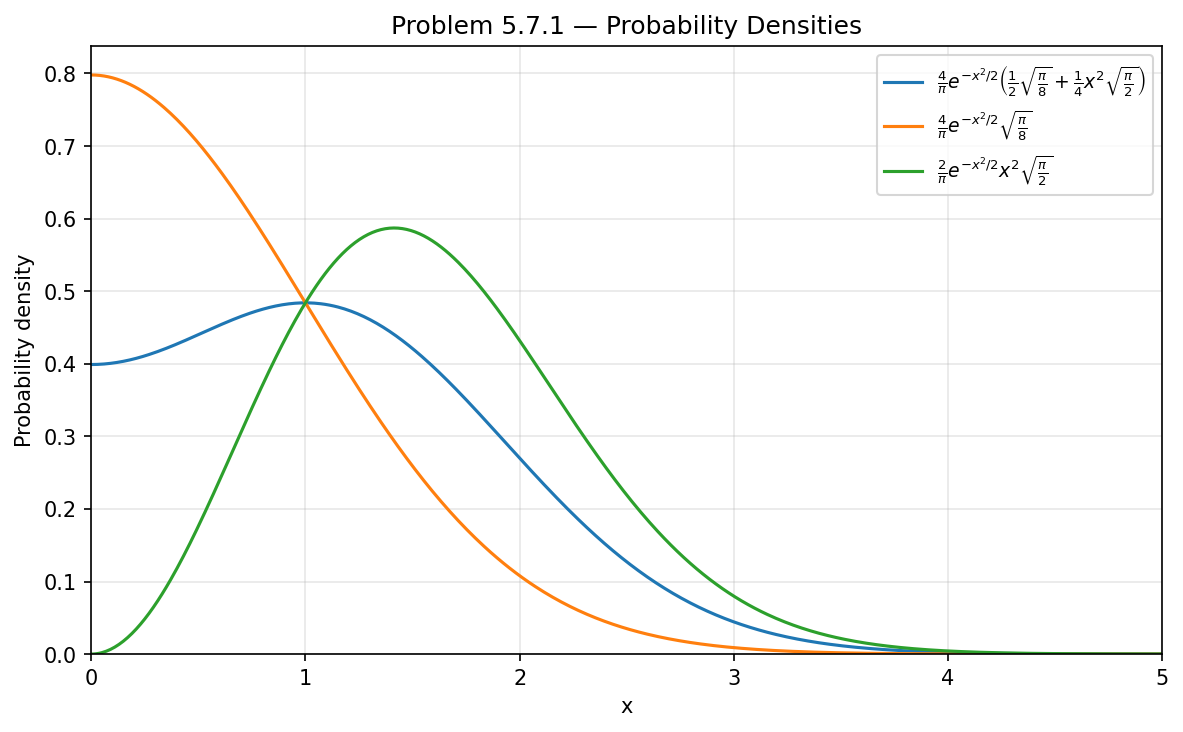
\includegraphics[width=0.8\textwidth,valign=t]{fig/prob5.7.1_densities.png}
    \item 
    Distinguishable:
    \begin{align*}
        \langle n(x)\rangle
        =&
        \frac{m\omega}{\pi\hbar}
        \frac{2m\omega}{\hbar}
        \int_{-\infty}^{\infty}\int_{-\infty}^{\infty}
        (\delta(x-x_1)+\delta(x-x_2))
        x_2^2
        e^{-\frac{m\omega}{\hbar}x_1^2}
        e^{-\frac{m\omega}{\hbar}x_2^2}dx_1dx_2\\
        =&
        \frac{2m^2\omega^2}{\pi\hbar^2}
        e^{-\frac{m\omega x^2}{\hbar}}
        \left[\int
        x_2^2e^{-\frac{m\omega}{\hbar}x_2^2}
        dx_2
        +
        \int
        x^2e^{-\frac{m\omega}{\hbar}x_1^2}
        dx_1
        \right]
        \\
        =&
        \frac{2m^2\omega^2}{\pi\hbar^2}
        e^{-\frac{m\omega x^2}{\hbar}}
        \left[
        \frac{1}{2}
        \sqrt{\frac{\pi}{(\frac{m\omega}{\hbar})^3}}
        +x^2
        \sqrt{\frac{\pi}{\frac{m\omega}{\hbar}}}
        \right]
    \end{align*}
    Bosons:
    \begin{align*}
        \langle n(x)\rangle=&
        \frac{1}{2}
        \frac{m\omega}{\pi\hbar}
        \frac{2m\omega}{\hbar}
        \int
        (\delta(x-x_1)+\delta(x-x_2))
        \left[
        x_2
        e^{-\frac{m\omega}{2\hbar}x_1^2}
        e^{-\frac{m\omega}{2\hbar}x_2^2}
        +
        x_1
        e^{-\frac{m\omega}{2\hbar}x_1^2}
        e^{-\frac{m\omega}{2\hbar}x_2^2}
        \right]^2dx_1dx_2\\
        =&
        \frac{m^2\omega^2}{\pi\hbar^2}
        \int
        (\delta(x-x_1)+\delta(x-x_2))e^{-\frac{m\omega}{\hbar}(x_1^2+x_2^2)}
        (x_1^2+2x_1x_2+x_2^2)dx_1dx_2\\
        =&
        \frac{m^2\omega^2}{\pi\hbar^2}
        \left[
        \int 
        e^{-\frac{m\omega}{\hbar}(x^2+x_2^2)}
        (x^2+2xx_2+x_2^2)dx_2
        +
        \int
        e^{-\frac{m\omega}{\hbar}(x_1^2+x^2)}
        (x_1^2+2x_1x+x^2)dx_1
        \right]\\
        =&
        \frac{m^2\omega^2}{\pi\hbar^2}
        e^{-\frac{m\omega x^2}{\hbar}}
        2\left[x^2\sqrt{\frac{\pi}{\frac{m\omega}{\hbar}}}
        +
        \frac{1}{2}
        \sqrt{\frac{\pi}{(\frac{m\omega}{\hbar})^3}}
        \right]
    \end{align*}
    Fermions:
    \begin{align*}
        \langle n(x)\rangle=&
        \frac{1}{2}
        \frac{m\omega}{\pi\hbar}
        \frac{2m\omega}{\hbar}
        \int
        (\delta(x-x_1)+\delta(x-x_2))
        \left[
        x_2
        e^{-\frac{m\omega}{2\hbar}x_1^2}
        e^{-\frac{m\omega}{2\hbar}x_2^2}
        -
        x_1
        e^{-\frac{m\omega}{2\hbar}x_1^2}
        e^{-\frac{m\omega}{2\hbar}x_2^2}
        \right]^2dx_1dx_2\\
        =&
        \frac{m^2\omega^2}{\pi\hbar^2}
        \int
        (\delta(x-x_1)+\delta(x-x_2))e^{-\frac{m\omega}{\hbar}(x_1^2+x_2^2)}
        (x_1^2-2x_1x_2+x_2^2)dx_1dx_2\\
        =&
        \frac{m^2\omega^2}{\pi\hbar^2}
        \left[
        \int 
        e^{-\frac{m\omega}{\hbar}(x^2+x_2^2)}
        (x^2-2xx_2+x_2^2)dx_2
        +
        \int
        e^{-\frac{m\omega}{\hbar}(x_1^2+x^2)}
        (x_1^2-2x_1x+x^2)dx_1
        \right]\\
        =&
        \frac{m^2\omega^2}{\pi\hbar^2}
        e^{-\frac{m\omega x^2}{\hbar}}
        2\left[x^2\sqrt{\frac{\pi}{\frac{m\omega}{\hbar}}}
        +
        \frac{1}{2}
        \sqrt{\frac{\pi}{(\frac{m\omega}{\hbar})^3}}
        \right]
    \end{align*}
    All three expected density operators are the same.
    
    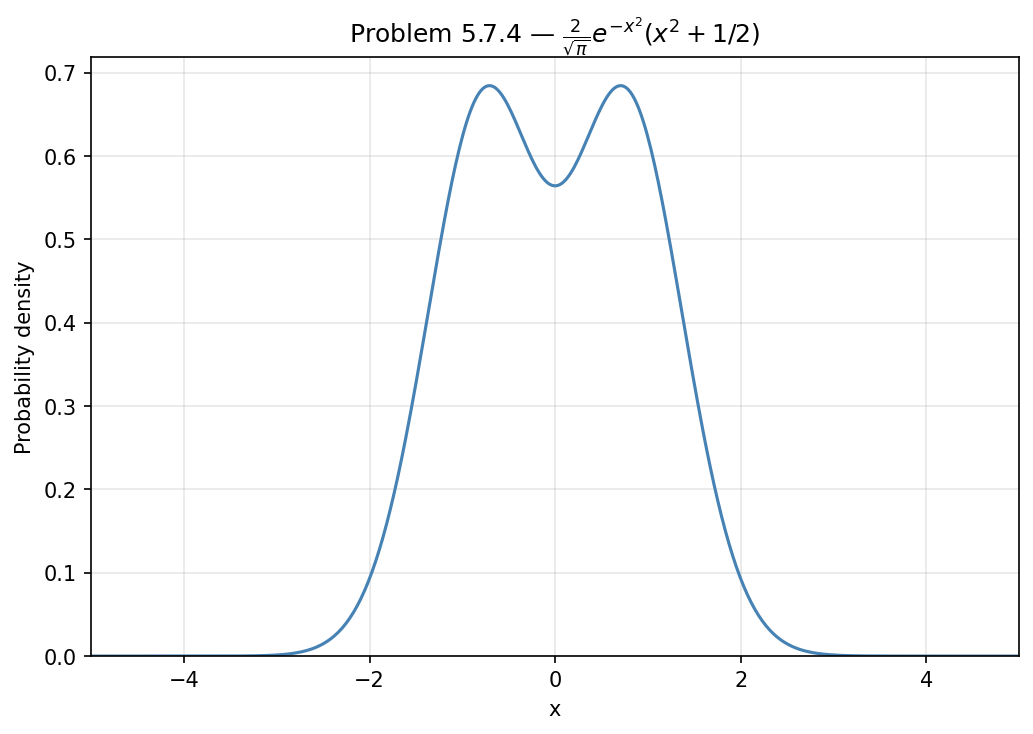
\includegraphics[width=0.8\textwidth,valign=t]{fig/prob5.7.4_density.png}
   \end{enumerate}
   \subsection*{Sol. 8}
   Distinguishable
   $$
   \psi_a(x_1)\psi_b(x_2)\psi_c(x_3)
   $$
   Bosons
   \begin{align*}
       &\psi_a(x_1)\psi_b(x_2)\psi_c(x_3) + 
       \psi_a(x_1)\psi_b(x_3)\psi_c(x_2) + 
       \psi_a(x_2)\psi_b(x_1)\psi_c(x_3)\\
       &+ 
       \psi_a(x_2)\psi_b(x_3)\psi_c(x_1) + 
       \psi_a(x_3)\psi_b(x_1)\psi_c(x_2)+ 
       \psi_a(x_3)\psi_b(x_2)\psi_c(x_1)
   \end{align*}
   Fermions
   \begin{align*}
       \begin{vmatrix}
       \psi_a(x_1) & \psi_b(x_1) & \psi_c(x_1)\\
       \psi_a(x_2) & \psi_b(x_2) & \psi_c(x_2)\\
       \psi_a(x_3) & \psi_b(x_3) & \psi_c(x_3)\\
       \end{vmatrix}=
       &\psi_a(x_1)\psi_b(x_2)\psi_c(x_3) + 
       \psi_a(x_3)\psi_b(x_1)\psi_c(x_2) + 
       \psi_a(x_2)\psi_b(x_3)\psi_c(x_1)\\
       &- 
       \psi_a(x_3)\psi_b(x_2)\psi_c(x_1) -
       \psi_a(x_2)\psi_b(x_1)\psi_c(x_3)-
       \psi_a(x_1)\psi_b(x_3)\psi_c(x_2)
   \end{align*}


   \subsection*{Sol. 9}
   \begin{enumerate}
       \item 
       The four lowest energy configuration for the infinite square well is 
   $$
   \psi_{11}|00\rangle,\;E=2K,\; d=1
   $$
   $$
   (\psi_{12}-\psi_{21})|11\rangle,\;
   (\psi_{12}-\psi_{21})|10\rangle,\;
   (\psi_{12}-\psi_{21})|1-1\rangle,\;
   (\psi_{12}+\psi_{21})|00\rangle
   E=5K,\;d=4
   $$
   $$
   \psi_{22}|00\rangle,\;
   E=8K,\;d=1
   $$
   $$
   (\psi_{13}-\psi_{31})|11\rangle,\;
   (\psi_{13}-\psi_{31})|10\rangle,\;
   (\psi_{13}-\psi_{31})|1-1\rangle,\;
   (\psi_{13}+\psi_{31})|00\rangle.\;
   E=10K,\;d=4
   $$
   \item 
   Note that the particle is a boson. By the CB table,
   the symmetric configurations are 
   $$
   |22\rangle, |21\rangle, |20\rangle, |00\rangle, |2-1\rangle, |2-2\rangle,
   $$
   and the anti-symmetric configurations are
   $$
   |11\rangle, |10\rangle, |1-1\rangle.
   $$

   The degeneracies for $2K$ is $6,$ 
   for $5K$ is $9,$ 
   for $8K$ is $6,$ 
   for $10K$ is $9.$ 
   \end{enumerate}
   \subsection*{Sol. 10}
   \begin{enumerate}
       \item By doing the anti-symmetry under 1 and 2,
       we have $a=b=g=h=0,$ and 
       $c=-e,$ $d=-f.$ Now we changes 2 and 3,
       we have $e=0=c,$ $d=0=f.$ Thus, such anti-symmetric configuration is impossible.
       \item The ground state energy is $6K$
       \begin{align*}
           &\begin{vmatrix}
               \psi_1(x_1)|\uparrow\rangle_1 & 
               \psi_1(x_1)|\downarrow\rangle_1 & 
               \psi_2(x_1)|\uparrow\rangle_1\\
               \psi_1(x_2)|\uparrow\rangle_2 & 
               \psi_1(x_2)|\downarrow\rangle_2 & 
               \psi_2(x_2)|\uparrow\rangle_2\\
               \psi_1(x_3)|\uparrow\rangle_3 & 
               \psi_1(x_3)|\downarrow\rangle_3 & 
               \psi_2(x_3)|\uparrow\rangle_3\\
           \end{vmatrix}\\
           =&
    \psi_1(x_1)\psi_1(x_2)\psi_2(x_3)|\uparrow\downarrow\uparrow\rangle
    +
    \psi_1(x_1)\psi_2(x_2)\psi_1(x_3)|\downarrow\uparrow\uparrow\rangle+
    \psi_2(x_1)\psi_1(x_2)\psi_1(x_3)|\uparrow\uparrow\downarrow\rangle
    \\&-
    \psi_2(x_1)\psi_1(x_2)\psi_1(x_3)|\uparrow\downarrow\uparrow\rangle
    -
    \psi_1(x_1)\psi_1(x_2)\psi_2(x_3)|\downarrow\uparrow\uparrow\rangle-
    \psi_1(x_1)\psi_2(x_2)\psi_1(x_3)|\uparrow\uparrow\downarrow\rangle
       \end{align*}
       \begin{align*}
           &\begin{vmatrix}
               \psi_1(x_1)|\uparrow\rangle_1 & 
               \psi_1(x_1)|\downarrow\rangle_1 & 
               \psi_2(x_1)|\downarrow\rangle_1\\
               \psi_1(x_2)|\uparrow\rangle_2 & 
               \psi_1(x_2)|\downarrow\rangle_2 & 
               \psi_2(x_2)|\downarrow\rangle_2\\
               \psi_1(x_3)|\uparrow\rangle_3 & 
               \psi_1(x_3)|\downarrow\rangle_3 & 
               \psi_2(x_3)|\downarrow\rangle_3\\
           \end{vmatrix}\\
           =&
    \psi_1(x_1)\psi_1(x_2)\psi_2(x_3)|\uparrow\downarrow\downarrow\rangle
    +
    \psi_1(x_1)\psi_2(x_2)\psi_1(x_3)|\downarrow\downarrow\uparrow\rangle+
    \psi_2(x_1)\psi_1(x_2)\psi_1(x_3)|\downarrow\uparrow\downarrow\rangle
    \\&-
    \psi_2(x_1)\psi_1(x_2)\psi_1(x_3)|\downarrow\downarrow\uparrow\rangle
    -
    \psi_1(x_1)\psi_1(x_2)\psi_2(x_3)|\downarrow\uparrow\downarrow\rangle-
    \psi_1(x_1)\psi_2(x_2)\psi_1(x_3)|\uparrow\downarrow\downarrow\rangle
       \end{align*}
       The degeneracy is 2.
       \item 
       \begin{align*}
           &\psi_1(x_1)\psi_1(x_2)\psi_2(x_3)|\uparrow\downarrow\uparrow\rangle
    +
    \psi_1(x_1)\psi_2(x_2)\psi_1(x_3)|\downarrow\uparrow\uparrow\rangle+
    \psi_2(x_1)\psi_1(x_2)\psi_1(x_3)|\uparrow\uparrow\downarrow\rangle
    \\&-
    \psi_2(x_1)\psi_1(x_2)\psi_1(x_3)|\uparrow\downarrow\uparrow\rangle
    -
    \psi_1(x_1)\psi_1(x_2)\psi_2(x_3)|\downarrow\uparrow\uparrow\rangle-
    \psi_1(x_1)\psi_2(x_2)\psi_1(x_3)|\uparrow\uparrow\downarrow\rangle\\
    =&\psi_1(x_1)\psi_1(x_2)
    (|\uparrow\downarrow\rangle -|\downarrow\uparrow\rangle)\psi_2(x_3)|\uparrow\rangle\\
    &
    +\psi_1(x_1)\psi_1(x_3)
    (-|\uparrow\downarrow\rangle_{13} +|\downarrow\uparrow\rangle_{13})\psi_2(x_3)|\uparrow\rangle_{2}
    +
    \psi_1(x_2)\psi_1(x_3)
    (|\uparrow\downarrow\rangle_{23} -|\downarrow\uparrow\rangle_{23})\psi_2(x_1)|\uparrow\rangle_{1}\\
    =&\Phi(1,2)\phi(3) -\Phi(1,3)\phi(2) + \Phi(2,3)\phi(1)
       \end{align*}
   \end{enumerate}
   \subsection*{Sol. 11}
   \begin{enumerate}
       \item Trivial
       \item 
       For $q=1,$ $N=3,$
       \begin{align*}
           \psi(z_1,z_2,z_3)
           =&
           A\left[
           (z_1-z_2)(z_1-z_3)(z_2-z_3)
           \right]
           \exp\left[
           -\frac{1}{2}
           (|z_1|^2+|z_2|^2+|z_3|^2)
           \right]\\
           =&
           A[z_1^2z_2-z_1^2z_3+z_1z_3^2-z_1z_2^2+z_2^2z_3-z_2z_3^2]
           \exp\left[
           -\frac{1}{2}
           (|z_1|^2+|z_2|^2+|z_3|^2)
           \right]\\
           =&
           A
           \begin{vmatrix}
           z_1^2e^{-\frac{1}{2}|z_1|^2} & z_1e^{-\frac{1}{2}|z_1|^2} & e^{-\frac{1}{2}|z_1|^2}\\
           z_2^2e^{-\frac{1}{2}|z_2|^2} & z_2e^{-\frac{1}{2}|z_2|^2} & e^{-\frac{1}{2}|z_2|^2}\\
           z_3^2e^{-\frac{1}{2}|z_3|^2} & z_3e^{-\frac{1}{2}|z_3|^2} & e^{-\frac{1}{2}|z_3|^2}\\
       \end{vmatrix}
       \end{align*}
       The states in which a single particle is occupied are $z^2e^{-\frac{1}{2}|z|^2},$
       $ze^{-\frac{1}{2}|z|^2},$ $e^{-\frac{1}{2}|z|^2}.$
       \item 
       For $q=3,$ $N=2,$
       \begin{align*}
           \psi(z_1,z_2,z_3)
           =&
           A
           (z_1-z_2)^3
           \exp\left[
           -\frac{1}{2}
           (|z_1|^2+|z_2|^2)
           \right]\\
           =&
           A[z_1^3-3z_1^2z_2+3z_1z_2^2-z_2^3]
           \exp\left[
           -\frac{1}{2}
           (|z_1|^2+|z_2|^2)
           \right]\\
           =&
           A
           \begin{vmatrix}
           z_1^3e^{-\frac{1}{2}|z_1|^2} & e^{-\frac{1}{2}|z_1|^2} \\
           z_2^3e^{-\frac{1}{2}|z_2|^2} & e^{-\frac{1}{2}|z_2|^2} 
       \end{vmatrix}
       +A
       \begin{vmatrix}
           -3z_1^2e^{-\frac{1}{2}|z_1|^2} & z_1e^{-\frac{1}{2}|z_1|^2} \\
           3z_2^2e^{-\frac{1}{2}|z_2|^2} & z_2e^{-\frac{1}{2}|z_2|^2} 
       \end{vmatrix}
       \end{align*}
       
       
   \end{enumerate}

   \subsection*{Sol. 12}
   \begin{enumerate}
       \item Note the Hamiltonian is symmetric in any $r,$ so any permutation of the arguments in the solution satisfies the equation. A completely symmetric function can then be constructed by adding all the $Z!$ terms together. For the anti-symmetry function, change the plus sign to a minus sign for any transposition(changing two labels only) it has done.

        If $\psi$ is symmetric in the first two terms, all the terms, fixing the third to the last terms, are canceled. For any $Z!$ terms, there is a term to let it get canceled, therefore, if any two terms are symmetric, the anti-symmetric function is not able to be construed.
        \item 
        There are only two possible spin states for an electron, by the pigeon hole principle, if $Z>2,$ there will be two electrons occupied in the same spin state, and is thus symmetric. By the argument above, there is no way to construct an anti-symmetry configuration.
        
   \end{enumerate}

   \subsection*{Sol. 13}
   \begin{enumerate}
       \item The total energy of two $n=2$ electrons is 
       $$
       4(-\frac{13.6}{4}-\frac{13.6}{4})=-27.2.
       $$
       The energy of the emitted electron would be 
       $$
       -27.2 - (-13.6)\times 4 = 27.2eV.
       $$
       \item 
       $$
       \frac{1}{\lambda}
       =4\mathcal{R}(\frac{1}{n_f^2}-\frac{1}{n_i^2})
       $$
   \end{enumerate}
   \subsection*{Sol. 14}
   \begin{enumerate}
       \item 
       For the ground state
       $$
       \psi_{100}(r_1)\psi_{100}(r_2),
       $$
       paired with a triplet configuration.
        For the excited state
       $$
       \psi_{nlm}(r_1)\psi_{100}(r_2)\pm \psi_{nlm}(r_2)\psi_{100}(r_1),
       $$
       paired with a triplet configuration if plus, and a singlet if minus.
        The energy level scheme is therefore $4(E_1+E_1)$ for the ground state, which is non-degenerate, and is $4(E_n+E_1)$ for the excited states, each having four degeneracies.
       \item  If those electrons are distinguishable, the energy schema would be $4(E_n+E_1),$ each having four degeneracies.
       
   \end{enumerate}
   \subsection*{Sol. 15}
   \begin{enumerate}
       \item 
       \begin{align*}
           &\int\frac{1}{|\bm r_1-\bm r_2|}
           \frac{64}{\pi^2 a^6}e^{-4(r_1+r_2)/a}d^3\bm r_1 d^3\bm r_2\\
           =&\frac{64}{\pi^2 a^6}
           \int\left[\frac{1}{\sqrt{r_1^2+r_2^2-2r_1r_2\cos\theta_2}} e^{-4r_2/a}r_2^2\sin\theta_2
           dr_2d\theta_2d\phi_2
           \right] e^{-4r_1/a}d^3\bm r_1
       \end{align*}
       \begin{align*}
           &2\pi\int_{0}^{\pi}
           \frac{1}{\sqrt{r_1^2+r_2^2-2r_1r_2\cos\theta_2}} e^{-4r_2/a}r_2^2\sin\theta_2
           d\theta_2\\
           =&
           2\pi e^{-4r_2/a}r_2^2\int_{r_1^2+r_2^2-2r_1r_2}^{r_1^2+r_2^2+2r_1r_2} \frac{1/(2r_1r_2)}{\sqrt{t}}dt\\
           =&2\pi e^{-4r_2/a}\frac{r_2}{r_1}
           \left(\sqrt{r_1^2+r_2^2+2r_1r_2} - \sqrt{r_1^2+r_2^2-2r_1r_2}\right)
       \end{align*}
       \begin{align*}
           &\int_{r_1}^{\infty}
           2\pi e^{-4r_2/a}\frac{r_2}{r_1}
           \left(\sqrt{r_1^2+r_2^2+2r_1r_2} - \sqrt{r_1^2+r_2^2-2r_1r_2}\right) dr_2\\
           =&2\pi\frac{1}{r_1}
           \int_{r_1}^{\infty}
           e^{-4r_2/a}r_2
           ((r_1+r_2)-(r_2-r_1))dr_2\\
        =&4\pi\int_{r_1}^{\infty}r_2e^{-4r_2/a}dr_2\\
        =&4\pi e^{-4r_2/a}\frac{-4/ar_2-1}{16/a^2}\bigg|^{\infty}_{r_1}\\
        =&\pi e^{-4r_1/a}(ar_1+\frac{1}{4}a^2)
       \end{align*}
       \begin{align*}
           &\int_{0}^{r_1}
           2\pi e^{-4r_2/a}\frac{r_2}{r_1}
           \left(\sqrt{r_1^2+r_2^2+2r_1r_2} - \sqrt{r_1^2+r_2^2-2r_1r_2}\right) dr_2\\
           =&2\pi\frac{1}{r_1}
           \int_{0}^{r_1}
           e^{-4r_2/a}r_2
           ((r_1+r_2)-(r_1-r_2))dr_2\\
        =&4\pi\frac{1}{r_1}\int_{0}^{r_1}r_2^2e^{-4r_2/a}dr_2\\
        =&4\pi\frac{1}{r_1} 
        e^{-4r_2/a}(\frac{r_2^2}{-4/a}-\frac{2r_2}{16/a^2}+\frac{2}{-64/a^3})\bigg|^{r_1}_{0}\\
        =&
        4\pi\frac{1}{r_1} 
        \left[e^{-4r_1/a}(\frac{r_1^2}{-4/a}-\frac{2r_1}{16/a^2}+\frac{2}{-64/a^3})
        -\frac{2}{-64/a^3}
        \right]\\
        =&\pi(e^{-4r_1/a}(-r_1a-\frac{1}{2}a^2-\frac{a^3}{8r_1})+\frac{a^3}{8r_1})
       \end{align*}
       \begin{align*}
           &\frac{64}{\pi^2 a^6}
           \int\left[
           \pi e^{-4r_1/a}(ar_1+\frac{1}{4}a^2)
           +
           \pi(e^{-4r_1/a}(-r_1a-\frac{1}{2}a^2-\frac{a^3}{8r_1})+\frac{a^3}{8r_1})
           \right]e^{-4r_1/a}r_1^2\sin\theta_1 dr_1d\theta_1d\phi_1\\
           =&
           \frac{64}{ a^6}4
           \int 
           \left[
           (e^{-4r_1/a}(-\frac{1}{4}a^2-\frac{a^3}{8r_1})+\frac{a^3}{8r_1})
           \right]e^{-4r_1/a}r_1^2 dr_1\\
           =&
           \frac{64}{ a^6}4
           \int 
           \left[
           -\frac{1}{4}e^{-8r_1/a}a^2r_1^2 
            -\frac{1}{8}e^{-8r_1/a}a^3r_1
            +\frac{1}{8}e^{-4r_1/a}a^3r_1
           \right] dr_1\\
           =&
           \frac{256}{a^6}
           \bigg[
           -\frac{1}{4}a^2
           e^{-8/ar_1}
           (\frac{r_1^2}{-8/a}-\frac{2r_1}{64/a^2}+\frac{2}{-512/a^3})
           \bigg|^\infty_0\\
           &-
           \frac{1}{8}
           a^3
           e^{-8/ar_1}(\frac{-8/ar_1-1}{64/a^2})
           \bigg|^\infty_0
           +\frac{1}{8}
           a^3e^{-4/ar_1}(\frac{-4/ar_1-1}{16/a^2})\bigg|^\infty_0
           \bigg]\\
           =&
           \frac{256}{a^6}
           \left[
           -a^2\frac{a^3}{1024}
           -a^3\frac{a^2}{512}
           +a^3\frac{a^2}{128}
           \right]=\frac{5}{4a}
       \end{align*}
       \item 
       The estimated repulsion energy is 
       $$
       \frac{1}{4\pi\epsilon_0}\frac{5e^2}{4a}\approx 
       34eV,
       $$
       approximately meets the gap between $-109eV$ to $-79eV.$
       
   \end{enumerate}

   \subsection*{Sol. 16}
   The energy of this state is 
   $$
   -13.6\times9\times 2 + (-13.6\times 9 / 4)
   = -275.4
   $$
   By problem 5.10, there are two degeneracies for this configuration.

   \subsection*{Sol. 17}
   \begin{enumerate}
       \item 
       H: $(1s)$

   He: $(1s)^2$

   Li: $(1s)^2(2s)$

   Be: $(1s)^2(2s)^2$

   B: $(1s)^2(2s)^2(2p)$

   C: $(1s)^2(2s)^2(2p)^2$

   N: $(1s)^2(2s)^2(2p)^3$

   O: $(1s)^2(2s)^2(2p)^4$

   F: $(1s)^2(2s)^2(2p)^5$

   Ne: $(1s)^2(2s)^2(2p)^6$

   \item 

   H: $ \prescript{2}{}{S}_{1/2} $

   He: $ \prescript{1}{}{S}_{0} $

   Li: $ \prescript{2}{}{S}_{1/2} $

   Be: $ \prescript{1}{}{S}_{0} $

   For Boron, the total orbital momenta could be $1,$ and the total spin momenta could be $\frac{1}{2},$ so the total momenta could be $\frac{3}{2}$ or $\frac{1}{2}.$

   For Carbon, the total orbital momenta could be $2,$ $1$ or $0,$ and the total spin momenta could be $1,$ or $0$ so the total momenta could be $3$, $2,$ $1$ or $0.$

    For Nitrogen, the total orbital momenta could be $3,$ $2,$ $1$ or $0,$ and the total spin momenta could be $\frac{3}{2},$ or $\frac{1}{2}$ so the total momenta could be $\frac{5}{2}$, $\frac{3}{2},$ or $\frac{1}{2}.$
   
   \end{enumerate}

   \subsection*{Sol. 18}
   \begin{enumerate}
       \item The excited states would be orthohelium, namely, a triplet configuration.
       \item 
       The Hund's first rule favors $S=1,$ which is symmetric, so the orbital state should be anti symmetric. $L=2$ is symmetric, so it will be $S=1,$ $L=1.$
       \item 
       Boron is no more than half filled, so $J=\frac{1}{2}.$
       \item 
       For Carbon, $S=1,$ $L=1,$ and it is no more than half filled, therefore $J=0.$

       For Nitrogen, $S=\frac{3}{2}.$
        From Slater's determinant: 
        \begin{align*}
            \begin{vmatrix}
                |11\rangle_1 & |10\rangle_1 & |1-1\rangle_1\\
                |11\rangle_2 & |10\rangle_2 & |1-1\rangle_2\\
                |11\rangle_3 & |10\rangle_3 & |1-1\rangle_3\\
            \end{vmatrix}
            =&|11\rangle_1|10\rangle_2|1-1\rangle_3
            +
            |10\rangle_1|1-1\rangle_2|11\rangle_3
            +|1-1\rangle_1|11\rangle_2|10\rangle_3\\
            &-|1-1\rangle_1|10\rangle_2|11\rangle_3
            -|10\rangle_1|11\rangle_2|1-1\rangle_3
            -|11\rangle_1|1-1\rangle_2|10\rangle_3,
        \end{align*}
        note that the anti-symmetric subspace is one-dimensional, thus
        restricting the possibility to the state $|00\rangle,$ so
       $L=0.$ It is no more than half filled, therefore $J=\frac{3}{2}.$

        
       
   \end{enumerate}
   \subsection*{Sol. 19}
   The total spin is $2,$ total orbital momenta is $6,$ and the grand total angular momenta is $8.$

   $$
   (1s)^2(2s)^2(2p)^6(3s)^2(3p)^6(3d)^{10}(4s)^2(4p)^6
   (4d)^{10}(5s)^2(5p)^6(4f)^{10}(6s)^2
   $$
   \subsection*{Sol. 20}
   \begin{align*}
       \frac{E_{tot}}{Nd}=
       \frac{\hbar^2(3\pi^2Nd)^{5/3}}{10\pi^2mNd}V^{-2/3}
   \end{align*}
   \begin{align*}
       E_F = \frac{\hbar^2}{2m}(3\rho\pi^2)^{2/3}
       =\frac{\hbar^2}{2m}(3\frac{Nd}{V}\pi^2)^{2/3}
   \end{align*}
   \begin{align*}
       \frac{E_{tot}}{NdE_F}
       =
       \frac{3}{5}
   \end{align*}

   \subsection*{Sol. 21}
   \begin{enumerate}
       \item 
       \begin{align*}
           E_F=&\frac{\hbar^2}{2m}(3\rho\pi^2)^{2/3}
           =\frac{(1.054\times10^{-34})^2}{2\times9.109\times10^{-31}}
           (3\frac{8.96/63.5\times 6.022\times10^{23}}{(0.01)^3}\pi^2)^{2/3}
           /(1.602\times 10^{-19}) eV\\
           \approx &7.04eV
       \end{align*}
       \item 
       \begin{align*}
           v = \frac{\hbar}{m}(3\rho\pi^2)^{1/3}\approx 1.57\times 10^6m/s
       \end{align*}
       Pretty safe to assume them to be nonrelativistic.
       \item $$T=81739K.$$
       \item 
       $$
       P = 3.834\times 10^{10}N/m^2.
       $$
   \end{enumerate}

   \subsection*{Sol. 22}
    $$
    E_F=\frac{(1.054\times 10^{-34})^2}
    {2\times3\times 1.66\times10^{-27}}
    (3\times82/(3\times 1.66\times10^{-27})\times\pi^2)^{2/3}
    =6.909\times 10^{-23}J
    $$
    $$
    T = 5K
    $$

   \subsection*{Sol. 23}
   \begin{align*}
       \frac{dP}{dV}
       =-k\frac{5}{3}\rho^{2/3}\frac{Nd}{V^2}
       =-k\frac{5}{3}\rho^{5/3}/V
       =-\frac{5}{3}P/V
   \end{align*}
   $$
   B = -V\frac{dP}{dV}
   =\frac{5}{3}P
   $$
   For copper 
   $$
   B = 6.39\times10^{10}
   $$

   \subsection*{Sol. 24}
   \begin{enumerate}
       \item 
       \begin{align*}
           \psi(x)
           =
           &A\sin(kx) + \frac{A\sin(ka)}{e^{iqa}-\cos(ka)}\cos(kx)\\
           =&
           \frac{A}{e^{iqa}-\cos(ka)}[\sin(kx)e^{iqa}-\sin(kx)\cos(ka)
           +\sin(ka)\cos(kx)]\\
           =&
           \frac{Ae^{iqa}}{e^{iqa}-\cos(ka)}
           [\sin(kx)+e^{-iqa}\sin(k(a-x))]
       \end{align*}
       \item 
       If $z=j\pi,$ 
        by equation 5.68
        $$
        B = e^{-iqa}B(-1)^j,
        $$
        and by equation 5.69
        $$
        kA-e^{-iqa}kA(-1)^j = \frac{2m\alpha}{\hbar^2}B.
        $$
        We must have $B=0,$ or $e^{-iqa}=(-1)^j.$ If $e^{-iqa}=(-1)^j,$ then $B=0,$ so either way $B=0.$
        Thus the wave function is $\psi(x)=\sin(kx).$ At the delta function, $\psi(0)=0.$
   \end{enumerate}

   \subsection*{Sol. 25}
   The lowest allowed $z=2.628,$ note that 
   $$
   E = \frac{\hbar^2k^2}{2m} = \frac{z^2\alpha}{2\beta a} = 0.345 eV.
   $$

   \subsection*{Sol. 26}
   For $E<0,$ 
   all the derivations are the same. By substituting the relation $ik=\kappa$ into equation 5.71, 
   we have 
   \begin{align*}
       \cos(qa) =& \cos(-i\kappa a) + \frac{m\alpha}{-\hbar^2i\kappa}\sin(-i\kappa a)\\
       =& \cos(iz) + \frac{m\alpha a}{\hbar^2i z}\sin(iz)\\
       =&\cosh z + \frac{m\alpha a}{\hbar^2 z}\sinh z\\
       =&\cosh z + \beta\frac{\sinh z}{z}.
   \end{align*}
   
    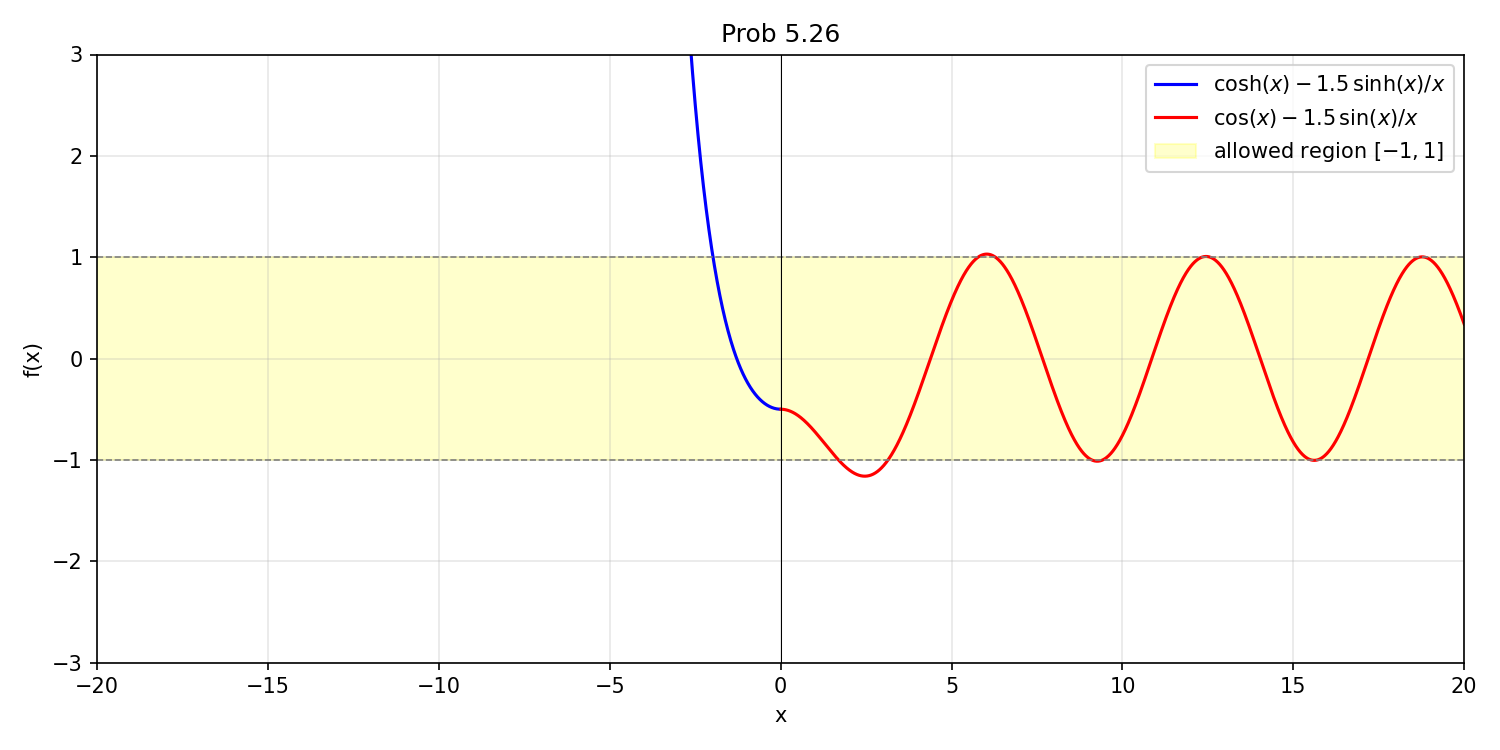
\includegraphics[width=0.8\textwidth,valign=t]{fig/prob5.26.png}
    
   There are $N$ states in the first band. 

   \subsection*{Sol. 27}
   For a given allowed value $k,$ equation 5.71 determines $\cos(qa).$ By recognizing $qa=\frac{2\pi n}{N},$ where $n=0,\dots,N-1$ as the angle of a circle, by symmetry, almost all $\cos(qa)$ corresponds to a pair of $n$s. Except when $\cos(qa)=\pm 1.$

   \subsection*{Sol. 28}
   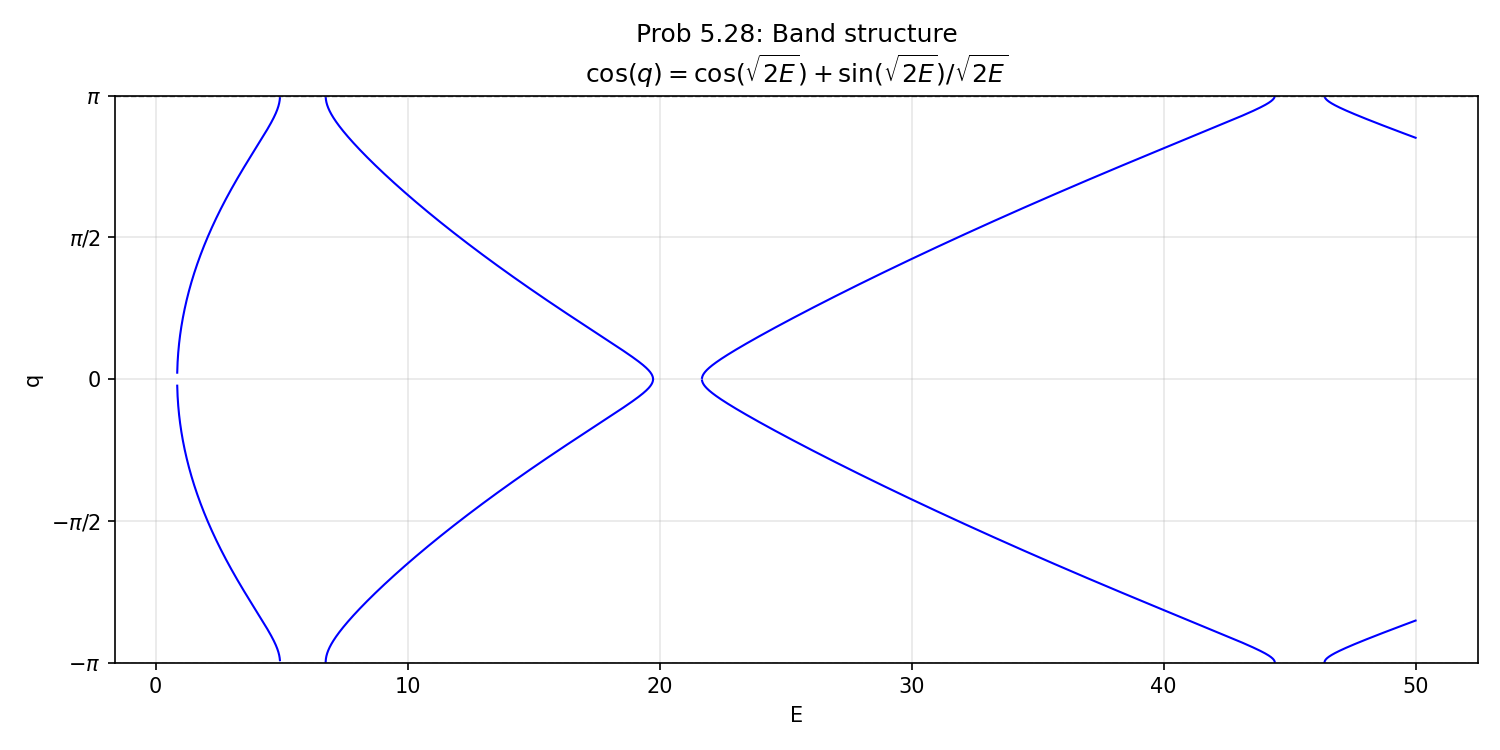
\includegraphics[width=0.8\textwidth,valign=t]{fig/prob5.28.png}

   \subsection*{Sol. 29}
   \begin{enumerate}
       \item 27 states if they are distinguishable.
       \item We can use the permanent method to construct the symmetric states. There would be $3+6+1=10$ possible states for identical bosons.
       \item Only 1 possible state if they are identical fermions.
   \end{enumerate}

   \subsection*{Sol. 30}
   $$
   \frac{1}{4}
   (\pi k_F^2)
   =\frac{Nd}{2}\frac{\pi^2}{A}\Rightarrow
   k_F=\sqrt{2\sigma\pi}
   $$
   $$
   E_F=\frac{\hbar^2\sigma\pi}{m}
   $$

   \subsection*{Sol. 31}
   An electron at the ground state of  a 3-dim infinite square well of width $a$ has energy $\frac{3\pi^2\hbar^2}{2ma^2}.$ So the total energy of $N$ isolated electrons is $\frac{3N\pi^2\hbar^2}{2ma^2}.$

   By equation 5.56, the total energy of all the filled state in a 3-dim square well of width $N^{1/3}a$ is 
   $$
   E=\frac{\hbar^2(3\pi^2N)^{5/3}}{10\pi^2m}(Na^3)^{-2/3}
   $$

   The cohesive energy per atom is thus 
   \begin{align*}
       \frac{3\pi^2\hbar^2}{2ma^2} - 
       \frac{\hbar^2(3\pi^2)^{5/3}}{10\pi^2ma^2}
       =&
       \frac{3\pi^2\hbar^2}{2ma^2}
       \left(1-\frac{3^{2/3}}{5\pi^{2/3}}\right).
   \end{align*}
    

   \subsection*{Sol. 32}
   \begin{enumerate}
       \item 
       \begin{align*}
       E_{tot}=\frac{1}{2}\frac{\hbar^2(3\pi^2 2N_+)^{5/3}}{10\pi^2m}V^{-2/3}
       +
       \frac{1}{2}\frac{\hbar^2(3\pi^2 2N_-)^{5/3}}{10\pi^2m}V^{-2/3}
   \end{align*}
   \item 
   \begin{align*}
       \frac{E_{tot}}{V}
       =&
       \frac{1}{2}\frac{\hbar^2(3\pi^2 2)^{5/3}}{10\pi^2m}
       V^{-5/3}
       \left[
       N_+^{5/3}
       +
       N_-^{5/3}
       \right]
   \end{align*}
   Note that 
   $$
   N_+=\frac{V}{2}\left(\rho-\frac{M}{\mu_B}\right),\; 
   N_-=\frac{V}{2}\left(\rho+\frac{M}{\mu_B}\right)
   $$
   \begin{align*}
       N_+^{5/3} + N_-^{5/3}
       =&\frac{V^{5/3}}{2^{5/3}}\left(\rho-\frac{M}{\mu_B}\right)^{5/3}
       +\frac{V^{5/3}}{2^{5/3}}\left(\rho+\frac{M}{\mu_B}\right)^{5/3}\\
       =&\frac{V^{5/3}}{2^{2/3}}\rho^{5/3}
       \left[1+\frac{5}{9}
       \left(\frac{M}{\mu_B\rho}\right)^2\right]
   \end{align*}
   \begin{align*}
       \frac{E_{tot}}{V}=&
       \frac{\hbar^2(3\pi^2 )^{5/3}}{10\pi^2m}\rho^{5/3}
       \left[1+\frac{5}{9}
       \left(\frac{M}{\mu_B\rho}\right)^2\right]
   \end{align*}
   \end{enumerate}
   \subsection*{Sol. 33}
   \begin{enumerate}
       \item 
       \begin{align*}
           \frac{E_{tot}}{V} =& \frac{\hbar^2(3\pi^2\rho)^{5/3}}{10\pi^2m}
           \left[
           1+\frac{5}{9}\left( \frac{M}{\rho\mu_B}\right)^2
           \right]
           +\frac{1}{V}\mu_BBN_+ - \frac{1}{V}\mu_B BN_-\\
           =&
           \frac{\hbar^2(3\pi^2\rho)^{5/3}}{10\pi^2m}
           \left[
           1+\frac{5}{9}\left( \frac{M}{\rho\mu_B}\right)^2
           \right]
           -BM
       \end{align*}
       $M$ reaches its minimum at 
       $$
       M=\frac{B}
       {\frac{\hbar^2(3\pi^2\rho)^{5/3}}{\pi^2m} \frac{1}{9}\frac{1}{\rho^2\mu_B^2}}.
       $$
       \item 
       \begin{align*}
           \chi = \mu_0
           \frac{1}
       {\frac{\hbar^2(3\pi^2\rho)^{5/3}}{\pi^2m} \frac{1}{9}\frac{1}{\rho^2\mu_B^2}}
       \approx 1.56969\times 10^{-5}.
       \end{align*}
   \end{enumerate}
   \subsection*{Sol. 34}
   \begin{enumerate}
       \item 
       \begin{align*}
           \Delta E = U\frac{V^2}{4}
           \left(\rho^2 - \frac{M^2}{\mu_B^2}\right)
       \end{align*}
       \item 
       \begin{align*}
           \frac{E_{tot}}{V} =& \frac{\hbar^2(3\pi^2\rho)^{5/3}}{10\pi^2m}
           \left[
           1+\frac{5}{9}\left( \frac{M}{\rho\mu_B}\right)^2
           \right]
           +U\frac{V}{4}
           \left(\rho^2 - \frac{M^2}{\mu_B^2}\right)\\
       \end{align*}
       To let the system favor non-zero $M,$ $U$ must be at least
       $$
       U=\frac{\hbar^2(3\pi^2\rho)^{5/3}}{10\pi^2m}
       \frac{20}{9\rho^2V}.
       $$
   \end{enumerate}
   \subsection*{Sol. 35}
   \begin{enumerate}
       \item 
       \begin{align*}
           E=\frac{\hbar^2(3\pi^2 Nd)^{5/3}}{10\pi^2m}(\frac{4}{3}\pi R^3)^{-2/3}
       \end{align*}
       \item 
       \begin{align*}
           U=-\frac{3}{5}\frac{G(NM)^2}{R}
       \end{align*}
       \item 
       \begin{align*}
           E_{tot} = &
           \frac{\hbar^2(3\pi^2 Nd)^{5/3}}{10\pi^2m}(\frac{4}{3}\pi R^3)^{-2/3} -\frac{3}{5}\frac{G(NM)^2}{R}
       \end{align*}
       The minimum happens at 
       \begin{align*}
           R =& \frac{2\frac{\hbar^2(3\pi^2 Nd)^{5/3}}{10\pi^2m}(\frac{4}{3}\pi )^{-2/3}}
           {\frac{3}{5}G(NM)^2}\\
           =&
           \frac{3^{4/3}}{4^{2/3}}\frac{\hbar^2\pi^{2/3}d^{5/3}}{GmN^{1/3}}
       \end{align*}
       Using $d = \frac{1}{2},$ $R=7.6\times 10^{25}N^{-1/3}m.$
       \item $$R = 7143.875km$$
       \item 
       $$
       E_F= 0.1942MeV
       $$
       The rest energy of an electron is $0.51MeV.$
   \end{enumerate}
   \subsection*{Sol. 36}
   \begin{enumerate}
       \item 
       \begin{align*}
           dE = \hbar ck\frac{V}{\pi^2}k^2 dk
       \end{align*}
       \begin{align*}
           E_{tot} = &
           \hbar c\frac{V}{\pi^2}\int_0^{k_F} 
           k^3dk\\
           =&
           \hbar c\frac{V}{\pi^2}\frac{1}{4}k_F^4\\
           =&\frac{\hbar c}{4\pi^2}(3\pi^2Nd)^{4/3}V^{-1/3}
       \end{align*}
       \item 
       \begin{align*}
           E = \frac{\hbar c}{4\pi^2}(3\pi^2Nd)^{4/3}(\frac{4}{3}\pi R^3)^{-1/3}
       \end{align*}
       \begin{align*}
           U = -\frac{3}{5}\frac{G(NM)^2}{R}
       \end{align*}

       \begin{align*}
           \frac{\hbar c}{4\pi^2}(3\pi^2N_cd)^{4/3}(\frac{4}{3}\pi R^3)^{-1/3}
           =\frac{3}{5}\frac{G(N_cM)^2}{R}
       \end{align*}
       \begin{align*}
           1.85059\times 10^{-26}N_c^{4/3} = 1.12343\times 10^{-64}N_c^{2}
           \Rightarrow 
           N_c = 2.04\times 10^{57}. 
       \end{align*}
       About $1.7$ mass of the sun.
       \item 
       \begin{align*}
           E = \frac{\hbar^2(3\pi^2 N)^{5/3}}{10\pi^2 M}(\frac{4}{3}\pi R^3)^{-2/3}
       \end{align*}
       \begin{align*}
           U = -\frac{3}{5}\frac{G(NM)^2}{R}
       \end{align*}
       The minimum occurs at 
       $$
       R = \frac{2\frac{\hbar^2(3\pi^2 N)^{5/3}}{10\pi^2 M}(\frac{4}{3}\pi )^{-2/3}}
       {\frac{3}{5}G(NM)^2}.
       $$ Using the mass of the sun, $R\approx 12.335km.$

       The Fermi energy is $56.237MeV.$ Compared to the rest energy of a neutron, $939.57MeV,$ it is reasonable to treat a neutron star nonrelativistaclly.
   \end{enumerate}
   \subsection*{Sol. 37}
   \begin{enumerate}
       \item 
       By equation 5.71, if $\alpha=0,$ $q=\frac{\sqrt{2mE}}{\hbar},$ thus
       \begin{align*}
           \frac{dq}{dE} = \frac{1}{\hbar}\frac{1}{2}(2mE)^{-1/2}2m
           =\frac{1}{\hbar}\sqrt{\frac{m}{2E}},
       \end{align*}
       and 
       $$
       \frac{1}{Na}G_{free}(E)
       =\frac{1}{\pi\hbar}\sqrt{\frac{m}{2E}}.
       $$
       \item 
       \begin{align*}
           -a\sin(qa)
           =-\sin(ka)ak'
           -\frac{m\alpha}{\hbar^2 k^2}k'
           \sin(ka)
           +\frac{m\alpha}{\hbar^2 k}\cos(ka)k'a
       \end{align*}
       $$
       \frac{dk}{dq} = \frac{dk}{dE}\frac{dE}{dq} = \frac{1}{\hbar}\sqrt{\frac{m}{2E}}\frac{dE}{dq}
       $$
       \begin{align*}
           \left|\frac{dE}{dq}\right| = 
           \hbar\sqrt{\frac{2E}{m}}
           \frac{a\sqrt{1-\left[\cos(ka)+\frac{m\alpha}{\hbar^2k}\sin(ka)\right]^2}}
           {|-\sin(ka)a-\frac{m\alpha}{\hbar^2k^2}\sin(ka)+\frac{m\alpha}{\hbar^2k}\cos(ka)a|}
       \end{align*}
       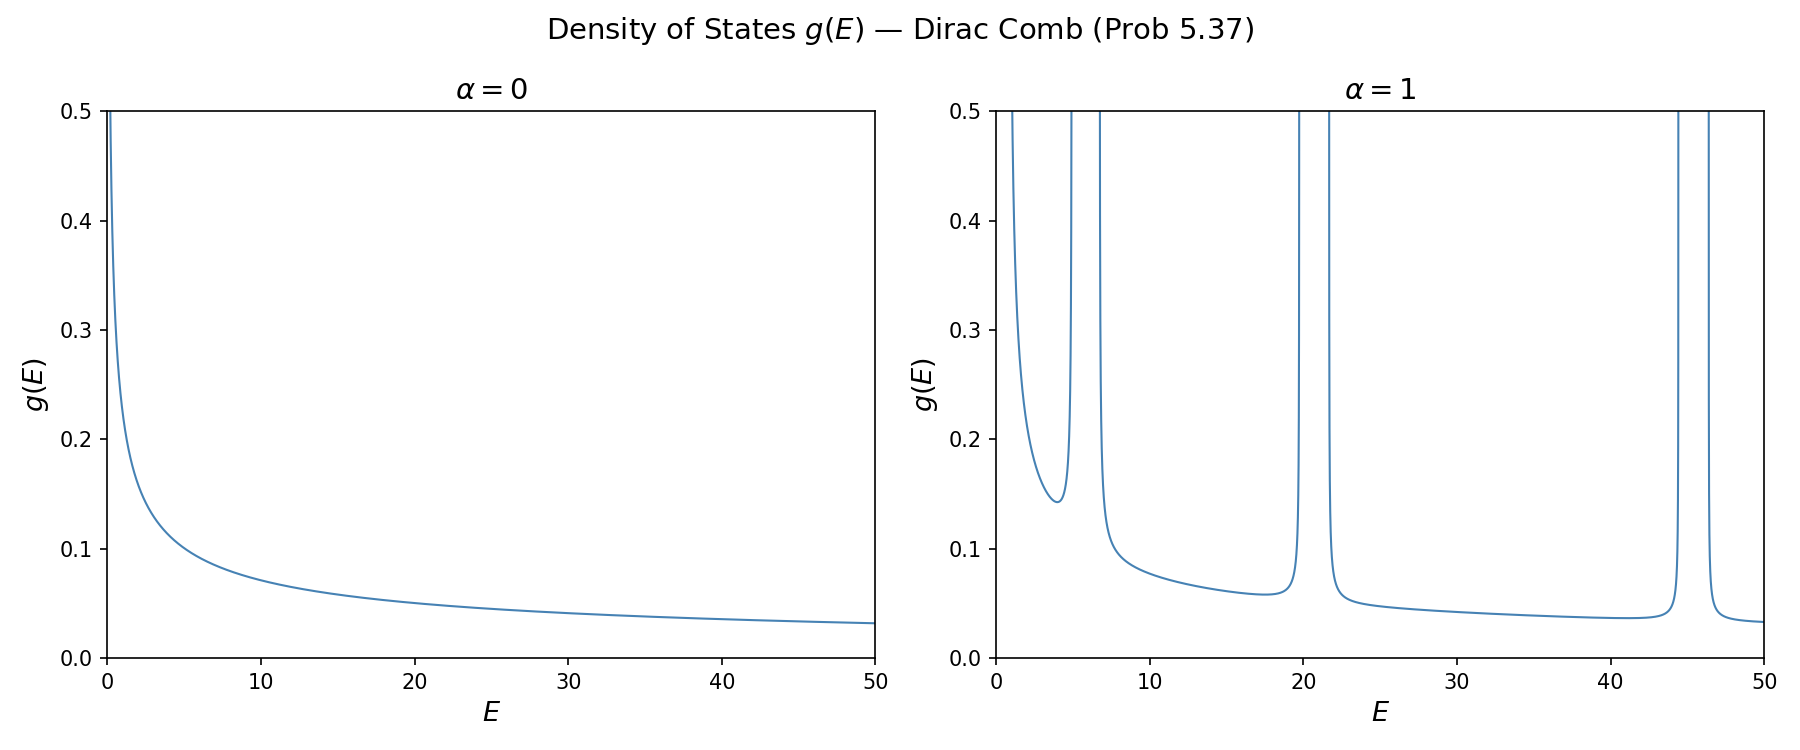
\includegraphics[width=0.8\textwidth,valign=t]{fig/prob5.37_dos.png}
   \end{enumerate}
   \subsection*{Sol. 38}
   \begin{enumerate}
       \item 
       \begin{align*}
           \frac{1}{N}
           \sum_{j=1}^N
           e^{i2\pi j(k-k')/N}
           = & 
           \frac{1}{N}
           \frac{e^{i2\pi(k-k')/N}(1-e^{i2\pi(k-k')})}{1-e^{i2\pi(k-k')/N}}
       \end{align*}
       If $k\neq k',$ the numerator is $0.$ If $k=k',$
       the sum directly says $1.$
    
        \begin{align*}
           \frac{1}{N}
           \sum_{j=1}^N
           e^{i2\pi j(k+k')/N}
           = & 
           \frac{1}{N}
           \frac{e^{i2\pi(k+k')/N}(1-e^{i2\pi(k+k')})}{1-e^{i2\pi(k+k')/N}},
       \end{align*}
       which equals $0$ except for $k+k'=N.$ If $k'=N-k,$ it equals $1.$

       \item 
       \begin{align*}
           [\hat a_{k-}, \hat a_{k'+}]
           =&\bigg[
           \frac{1}{\sqrt{N}}
           \sum_{j=1}^N e^{-i2\pi jk /N}
           \left(\sqrt{\frac{m\omega_k}{2\hbar}}x_j+
           \sqrt{\frac{\hbar}{2m\omega_k}}\frac{\partial}{\partial x_j}\right),\\
           &\frac{1}{\sqrt{N}}
           \sum_{s=1}^N e^{i2\pi sk' /N}
           \left(\sqrt{\frac{m\omega_{k'}}{2\hbar}}x_s-
           \sqrt{\frac{\hbar}{2m\omega_{k'}}}\frac{\partial}{\partial x_s}\right)
           \bigg]\\
           =&
           \frac{1}{N}
           \sum_{s,j=1}^N
           e^{-i2\pi jk /N}
           e^{i2\pi sk' /N}
           (
            -\sqrt{\frac{m\omega_k}{2\hbar}}\sqrt{\frac{\hbar}{2m\omega_{k'}}}
            [x_j, \frac{\partial}{\partial x_s}]
           +\sqrt{\frac{m\omega_{k'}}{2\hbar}}\sqrt{\frac{\hbar}{2m\omega_{k}}}
           [\frac{\partial}{\partial x_j}, x_s]
           )\\
           =&
           \frac{1}{N}
           \sum_{j=1}^N
           e^{i2\pi j(k'-k)/N}
            (
            \sqrt{\frac{\omega_k}{4\omega_{k'}}}
           +\sqrt{\frac{\omega_{k'}}{4\omega_k}}
           )\\
           =&\delta_{k,k'}.
       \end{align*}
       \begin{align*}
           [\hat a_{k-}, \hat a_{k'-}]
           =&\bigg[
           \frac{1}{\sqrt{N}}
           \sum_{j=1}^N e^{-i2\pi jk /N}
           \left(\sqrt{\frac{m\omega_k}{2\hbar}}x_j+
           \sqrt{\frac{\hbar}{2m\omega_k}}\frac{\partial}{\partial x_j}\right),\\
           &\frac{1}{\sqrt{N}}
           \sum_{s=1}^N e^{i2\pi sk' /N}
           \left(\sqrt{\frac{m\omega_{k'}}{2\hbar}}x_s+
           \sqrt{\frac{\hbar}{2m\omega_{k'}}}\frac{\partial}{\partial x_s}\right)
           \bigg]\\
           =&
           \frac{1}{N}
           \sum_{s,j=1}^N
           e^{-i2\pi jk /N}
           e^{i2\pi sk' /N}
           (
            \sqrt{\frac{m\omega_k}{2\hbar}}\sqrt{\frac{\hbar}{2m\omega_{k'}}}
            [x_j, \frac{\partial}{\partial x_s}]
           +\sqrt{\frac{m\omega_{k'}}{2\hbar}}\sqrt{\frac{\hbar}{2m\omega_{k}}}
           [\frac{\partial}{\partial x_j}, x_s]
           )\\
           =&
           \frac{1}{N}
           \sum_{j=1}^N
           e^{i2\pi j(k'-k)/N}
            (
            -\sqrt{\frac{\omega_k}{4\omega_{k'}}}
           +\sqrt{\frac{\omega_{k'}}{4\omega_k}}
           )\\
           =&0.
       \end{align*}
       \begin{align*}
           [\hat a_{k+}, \hat a_{k'+}]
           =&\bigg[
           \frac{1}{\sqrt{N}}
           \sum_{j=1}^N e^{-i2\pi jk /N}
           \left(\sqrt{\frac{m\omega_k}{2\hbar}}x_j-
           \sqrt{\frac{\hbar}{2m\omega_k}}\frac{\partial}{\partial x_j}\right),\\
           &\frac{1}{\sqrt{N}}
           \sum_{s=1}^N e^{i2\pi sk' /N}
           \left(\sqrt{\frac{m\omega_{k'}}{2\hbar}}x_s-
           \sqrt{\frac{\hbar}{2m\omega_{k'}}}\frac{\partial}{\partial x_s}\right)
           \bigg]\\
           =&
           \frac{1}{N}
           \sum_{s,j=1}^N
           e^{-i2\pi jk /N}
           e^{i2\pi sk' /N}
           (
            -\sqrt{\frac{m\omega_k}{2\hbar}}\sqrt{\frac{\hbar}{2m\omega_{k'}}}
            [x_j, \frac{\partial}{\partial x_s}]
           -\sqrt{\frac{m\omega_{k'}}{2\hbar}}\sqrt{\frac{\hbar}{2m\omega_{k}}}
           [\frac{\partial}{\partial x_j}, x_s]
           )\\
           =&
           \frac{1}{N}
           \sum_{j=1}^N
           e^{i2\pi j(k'-k)/N}
            (
            \sqrt{\frac{\omega_k}{4\omega_{k'}}}
           -\sqrt{\frac{\omega_{k'}}{4\omega_k}}
           )\\
           =&0.
       \end{align*}
    \item 
    \begin{align*}
        &\hat a_{k-}+ \hat a_{N-k+}\\
        =& 
        \frac{1}{\sqrt{N}}
        \left(
        e^{-i2\pi k/N}
        \left[
        \sqrt{\frac{m\omega_k}{2\hbar}}x_1
        +
        \sqrt{\frac{\hbar}{2m\omega_k}}\frac{\partial}{\partial x_1}
        \right]
        +\dots 
        +
        e^{-i2\pi Nk/N}
        \left[
        \sqrt{\frac{m\omega_k}{2\hbar}}x_N
        +
        \sqrt{\frac{\hbar}{2m\omega_k}}\frac{\partial}{\partial x_N}
        \right]
        \right)\\
        +&
        \frac{1}{\sqrt{N}}
        \bigg(
        e^{i2\pi (N-k)/N}
        \left[
        \sqrt{\frac{m\omega_{N-k}}{2\hbar}}x_1
        -
        \sqrt{\frac{\hbar}{2m\omega_{N-k}}}\frac{\partial}{\partial x_1}
        \right]\\
        &+\dots 
        +
        e^{i2\pi N(N-k)/N}
        \left[
        \sqrt{\frac{m\omega_{N-k}}{2\hbar}}x_N
        -
        \sqrt{\frac{\hbar}{2m\omega_{N-k}}}\frac{\partial}{\partial x_N}
        \right]
        \bigg)\\
        =&
        \frac{1}{\sqrt{N}}
        \left(
        e^{-i2\pi k/N}
        \left[
        \sqrt{\frac{m\omega_k}{2\hbar}}x_1
        +
        \sqrt{\frac{\hbar}{2m\omega_k}}\frac{\partial}{\partial x_1}
        \right]
        +\dots 
        +
        e^{-i2\pi Nk/N}
        \left[
        \sqrt{\frac{m\omega_k}{2\hbar}}x_N
        +
        \sqrt{\frac{\hbar}{2m\omega_k}}\frac{\partial}{\partial x_N}
        \right]
        \right)\\
        +&
        \frac{1}{\sqrt{N}}
        \bigg(
        e^{-i2\pi k/N}
        \left[
        \sqrt{\frac{m\omega_{k}}{2\hbar}}x_1
        -
        \sqrt{\frac{\hbar}{2m\omega_{k}}}\frac{\partial}{\partial x_1}
        \right]
        +\dots +
        e^{-i2\pi Nk/N}
        \left[
        \sqrt{\frac{m\omega_k}{2\hbar}}x_N
        -
        \sqrt{\frac{\hbar}{2m\omega_k}}\frac{\partial}{\partial x_N}
        \right]
        \bigg)\\
        =&
        \frac{2}{\sqrt{N}}
        \sqrt{\frac{m\omega_k}{2\hbar}}
        \sum_{s=1}^N
        e^{-i2\pi sk/N}
        x_s
    \end{align*}
    \begin{align*}
    R + \frac{1}{\sqrt{N}}\sum_{k=1}^{N-1}\sqrt{\frac{\hbar}{2 m\omega_k}}(\hat a_{k-}+ \hat a_{N-k+})e^{i2\pi jk/N}
    = & 
    R+ \frac{1}{\sqrt{N}}\sum_{k=1}^{N-1}\frac{1}{\sqrt{N}}
    \sum_{s=1}^Nx_s e^{i2\pi (j-s)k/N}
    \\
    = & R+ \frac{1}{N}\sum_{s=1}^Nx_s (N\delta_{j,s} - 1)\\
    =& x_j
    \end{align*}



    \begin{align*}
        &\hat a_{k-}- \hat a_{N-k+}\\
        =& 
        \frac{1}{\sqrt{N}}
        \left(
        e^{-i2\pi k/N}
        \left[
        \sqrt{\frac{m\omega_k}{2\hbar}}x_1
        +
        \sqrt{\frac{\hbar}{2m\omega_k}}\frac{\partial}{\partial x_1}
        \right]
        +\dots 
        +
        e^{-i2\pi Nk/N}
        \left[
        \sqrt{\frac{m\omega_k}{2\hbar}}x_N
        +
        \sqrt{\frac{\hbar}{2m\omega_k}}\frac{\partial}{\partial x_N}
        \right]
        \right)\\
        -&
        \frac{1}{\sqrt{N}}
        \bigg(
        e^{i2\pi (N-k)/N}
        \left[
        \sqrt{\frac{m\omega_{N-k}}{2\hbar}}x_1
        -
        \sqrt{\frac{\hbar}{2m\omega_{N-k}}}\frac{\partial}{\partial x_1}
        \right]\\
        &+\dots 
        +
        e^{i2\pi N(N-k)/N}
        \left[
        \sqrt{\frac{m\omega_{N-k}}{2\hbar}}x_N
        -
        \sqrt{\frac{\hbar}{2m\omega_{N-k}}}\frac{\partial}{\partial x_N}
        \right]
        \bigg)\\
        =&
        \frac{1}{\sqrt{N}}
        \left(
        e^{-i2\pi k/N}
        \left[
        \sqrt{\frac{m\omega_k}{2\hbar}}x_1
        +
        \sqrt{\frac{\hbar}{2m\omega_k}}\frac{\partial}{\partial x_1}
        \right]
        +\dots 
        +
        e^{-i2\pi Nk/N}
        \left[
        \sqrt{\frac{m\omega_k}{2\hbar}}x_N
        +
        \sqrt{\frac{\hbar}{2m\omega_k}}\frac{\partial}{\partial x_N}
        \right]
        \right)\\
        -&
        \frac{1}{\sqrt{N}}
        \bigg(
        e^{-i2\pi k/N}
        \left[
        \sqrt{\frac{m\omega_{k}}{2\hbar}}x_1
        -
        \sqrt{\frac{\hbar}{2m\omega_{k}}}\frac{\partial}{\partial x_1}
        \right]
        +\dots +
        e^{-i2\pi Nk/N}
        \left[
        \sqrt{\frac{m\omega_k}{2\hbar}}x_N
        -
        \sqrt{\frac{\hbar}{2m\omega_k}}\frac{\partial}{\partial x_N}
        \right]
        \bigg)\\
        =&
        \frac{2}{\sqrt{N}}
        \sqrt{\frac{\hbar}{2m\omega_k}}
        \sum_{s=1}^N
        e^{-i2\pi sk/N}
        \frac{\partial}{\partial x_s}
    \end{align*}
    The transformation goes by $R = \frac{x_1+\dots+x_N}{N},$ 
    $r_1=\frac{x_1-x_2}{N},\dots, r_{N}=\frac{x_1-x_N}{N},$ then
    $$
    x_1 = R + r_2 + r_3+\dots + r_{N-1}
    $$
    $$
    x_2 = R - r_2 + (r_3-r_2)+\dots + (r_{N-1}-r_2)
    $$
    $$
    \vdots
    $$
    $$
    x_N = R - (r_2-r_N) + (r_3-r_N)+\dots + (r_{N-1}-r_N),
    $$
    then
    $$\frac{\partial}{\partial R}=\frac{\partial }{\partial x_1}
    \frac{\partial x_1}{\partial R}+
    \dots +\frac{\partial }{\partial x_N}\frac{\partial x_N}{\partial R}
    =\frac{\partial }{\partial x_1}+
    \dots +\frac{\partial }{\partial x_N}.
    $$
    Thus
    \begin{align*}
        \frac{1}{N}\frac{\partial}{\partial R}
        +\frac{1}{\sqrt{N}}
        \sum_{k=1}^{N-1}
        \sqrt{\frac{m\omega_k}{2\hbar}}
        (\hat a_{k-}- \hat a_{N-k+}) e^{i2\pi jk/N}   
        =& 
        \frac{1}{N}\frac{\partial}{\partial R}+
        \frac{1}{N}
        \sum_{k=1}^{N-1}\sum_{s=1}^N
        e^{i2\pi(j-s)k/N}
        \frac{\partial}{\partial x_s}\\
        =&\frac{1}{N}\frac{\partial}{\partial R}+
        \frac{1}{N}
        \sum_{s=1}^N\frac{\partial}{\partial x_s}(N\delta_{j,s}-1)\\
        =&\frac{\partial}{\partial x_j}
    \end{align*}
    

    \item 
    \begin{align*}
        &\hat a_{k+}\hat a_{k-}\\
        =&
        \frac{1}{\sqrt{N}}
        \left(
        e^{i2\pi k/N}
        \left[
        \sqrt{\frac{m\omega_k}{2\hbar}}x_1
        -
        \sqrt{\frac{\hbar}{2m\omega_k}}\frac{\partial}{\partial x_1}
        \right]
        +\dots 
        +
        e^{i2\pi Nk/N}
        \left[
        \sqrt{\frac{m\omega_k}{2\hbar}}x_N
        -
        \sqrt{\frac{\hbar}{2m\omega_k}}\frac{\partial}{\partial x_N}
        \right]
        \right)\\
        &\frac{1}{\sqrt{N}}
        \left(
        e^{-i2\pi k/N}
        \left[
        \sqrt{\frac{m\omega_k}{2\hbar}}x_1
        +
        \sqrt{\frac{\hbar}{2m\omega_k}}\frac{\partial}{\partial x_1}
        \right]
        +\dots 
        +
        e^{-i2\pi Nk/N}
        \left[
        \sqrt{\frac{m\omega_k}{2\hbar}}x_N
        +
        \sqrt{\frac{\hbar}{2m\omega_k}}\frac{\partial}{\partial x_N}
        \right]
        \right)
    \end{align*}

    There are three kinds of terms:
    \begin{align*}
        e^{i2\pi jk/N}
        \sqrt{\frac{m\omega_k}{2\hbar}}x_j
        e^{-i2\pi sk/N}
        \sqrt{\frac{m\omega_k}{2\hbar}}x_s
        =\frac{m\omega_k}{2\hbar}
        e^{i2\pi (j-s)k/N}
        x_jx_s
    \end{align*}
    \begin{align*}
        &e^{i2\pi jk/N}
        \sqrt{\frac{m\omega_k}{2\hbar}}x_j
        e^{-i2\pi sk/N}
        \sqrt{\frac{\hbar}{2m\omega_k}}\frac{\partial}{\partial x_s}
        -
        e^{i2\pi sk/N}
        \sqrt{\frac{\hbar}{2m\omega_k}}
        \frac{\partial}{\partial x_s}
        e^{-i2\pi jk/N}
        \sqrt{\frac{m\omega_k}{2\hbar}}x_j
        \\
        =&
        \frac{1}{2}e^{i2\pi(j-s)k/N}x_j\frac{\partial}{\partial x_s}
        -\frac{1}{2}e^{i2\pi(s-j)k/N}x_j\frac{\partial}{\partial x_s}
        -\frac{1}{2}e^{i2\pi(s-j)k/N}\delta_{s,j}\\
        =&i\sin(2\pi(j-s)k/N)x_j\frac{\partial}{\partial x_s}
        -\frac{1}{2}\delta_{s,j}
    \end{align*}

    \begin{align*}
        -e^{i2\pi jk/N}
        \sqrt{\frac{\hbar}{2m\omega_k}}\frac{\partial}{\partial x_j}
        e^{-i2\pi sk/N}
        \sqrt{\frac{\hbar}{2m\omega_k}}\frac{\partial}{\partial x_s}
        =-\frac{\hbar}{2m\omega_k}
        e^{i2\pi (j-s)k/N}
        \frac{\partial}{\partial x_j}\frac{\partial}{\partial x_s}.
    \end{align*}
    Note that
    \begin{align*}
        \sum_{k=1}^{N-1}
        \hbar\omega_k
        \frac{m\omega_k}{2\hbar}
        e^{i2\pi (j-s)k/N}
        x_jx_s
        =&
        -\frac{m}{2}
        x_jx_s 
        \frac{4\omega^2}{4}
        \sum_{k=1}^{N-1}
        (e^{2i(\pi k /N)}
        -2+
        e^{-2i(\pi k /N)})
        e^{i2\pi (j-s)k/N}\\
        =&
        -\frac{m}{2}
        x_jx_s 
        \omega^2
        \left[
        N\delta_{j+1,s+nN} - 1
        -2N\delta_{j,s} + 2
        +N\delta_{j+nN,s+1} - 1
        \right]
    \end{align*}
    \begin{align*}
         &\sum_{k=1}^{N-1}\hbar \omega_k
        [i\sin(2\pi(j-s)k/N)x_j\frac{\partial}{\partial x_s}
        -\frac{1}{2}\delta_{s,j}]
    \end{align*}
    Since, $\omega_k = \omega_{N-k},$ $\sin(2\pi(j-s)k/N)=-\sin(2\pi(j-s)(N-k)/N),$ the first term got canceled.
    
    
    \begin{align*}
        -\sum_{k=1}^{N-1}
        \hbar\omega_k 
        \frac{\hbar}{2m\omega_k}
        e^{i2\pi (j-s)k/N}
        \frac{\partial}{\partial x_j}\frac{\partial}{\partial x_s}
        =&
        -\frac{\hbar^2}{2m}\frac{\partial^2}{\partial x_j\partial x_s}(N\delta_{j,s}-1)
    \end{align*}
    So 
    \begin{align*}
        \sum_{k=1}^{N-1}\hbar\omega_k(\hat a_{k+}\hat a_{k-} + \frac{1}{2} )
        = & \frac{1}{N}\bigg(\sum_{s,j}
        -\frac{m}{2}
        x_jx_s 
        \omega^2
        \left[
        N\delta_{j+1,s} 
        -2N\delta_{j,s} 
        +N\delta_{j,s+1} 
        \right]\\
         & -\frac{1}{2}\hbar\delta_{s,j}\sum_{k=1}^{N-1}\omega_k
        -\frac{\hbar^2}{2m}\frac{\partial^2}{\partial x_j\partial x_s}(N\delta_{j,s}-1)
        \bigg) + \frac{1}{2}\hbar\sum_{k=1}^{N-1}\omega_k
    \end{align*}

    \begin{align*}
        & \sum_{s,j}
        -\frac{m}{2}
        x_jx_s 
        \omega^2
        \left[
        N\delta_{j+1,s+nN} 
        -2N\delta_{j,s} 
        +N\delta_{j+nN,s+1} 
        \right] \\
        = & 
        - \frac{m}{2}\omega^2N 
        (-2x_1^2-2x_2^2-\dots-2x_N^2 + 2x_1x_2 + 2x_2x_3 + \dots +2 x_{N}x_{N+1})\\
        =& \frac{m}{2}\omega^2N[(x_2-x_1)^2 + (x_3-x_2)^2 + \dots + (x_{N+1}-x_{N})^2]
    \end{align*}
    \begin{align*}
        -\frac{\hbar^2}{2(Nm)}\frac{\partial^2}{\partial R^2}
        =-\frac{\hbar^2}{2Nm}\sum_{s,j}\frac{\partial^2}{\partial x_s\partial x_j}.
    \end{align*}
    Hence 
    \begin{align*}
        &-\frac{\hbar^2}{2(Nm)}\frac{\partial^2}{\partial R^2} + \sum_{k=1}^{N-1}
        \hbar \omega_k(\hat a_{k+}\hat a_{k-} + \frac{1}{2})\\
        =& 
        -\frac{\hbar^2}{2Nm}\sum_{s,j}\frac{\partial^2}{\partial x_s\partial x_j}
        +\frac{\hbar^2}{2Nm}\sum_{s,j}\frac{\partial^2}{\partial x_s\partial x_j} 
        -\frac{\hbar^2}{2m}\sum_{j}\frac{\partial^2}{\partial x_j^2}\\
         &+ \frac{m}{2}\omega^2[(x_2-x_1)^2 + (x_3-x_2)^2 + \dots + (x_{N+1}-x_{N})^2]\\
         =& \hat H.
    \end{align*}

   

       
   \end{enumerate}
   \subsection*{Sol. 39}
   \begin{enumerate}
       \item 
       $$
       e^{i(k_x(x+l_x)+k_y y + k_zz)}
       =e^{i(k_xx+k_yy+k_zz)}
       \Rightarrow k_xl_x=2n_x\pi,
       $$
       similarly 
       $$
       k_yl_y = 2n_y\pi
       $$
       $$
       k_zl_z = 2n_z\pi.
       $$
       The k space volume is 
       $$
       \frac{2\pi}{l_x}
       \frac{2\pi}{l_y}
       \frac{2\pi}{l_z} = \frac{8\pi^3}{V}
       $$
       \item 
       $$
       \frac{4}{3}\pi k_F^3 = \frac{Nd}{2}\frac{8\pi^3}{V}
       \Rightarrow k_F = 
       (3\rho\pi^2)^{1/3}
       $$
       The rest are all the same. 
       
   \end{enumerate}

\section{Symmetries and Conservation Laws}
\subsection*{Sol. 1}
\begin{enumerate}
    \item It is equivalent to a reflection over the $xy$ plane, followed by a $\pi$ rotation along the $z$ axis.
     That is 
     $$
     RM\psi(x,y,z) = R\psi(x,y,-z) = \psi(-x,-y,-z)
     $$
     \item 
     \begin{align*}
         r\sin(\pi-\theta)\cos(\phi+\pi)
         =-r\sin\theta\cos\phi=-x
     \end{align*}
     \begin{align*}
         r\sin(\pi-\theta)\sin(\phi+\pi)
         =-r\sin\theta\sin\phi=-y
     \end{align*}
     \begin{align*}
         r\cos(\pi-\theta)
         =-r\cos\theta=-z
     \end{align*}
     \item 
     \begin{align*}
         \psi_{nlm}(r,\pi-\theta,\phi+\pi)
         =&R_{nl}(r)Y_{lm}(\pi,\pi-\theta, \phi+\pi)\\
         =&R_{nl}(r)\sqrt{\frac{(2l+1)}{4\pi}\frac{(l-m)!}{(l+m)!}}e^{im(\phi+\pi)}
         P^m_l(\cos(\pi-\theta))\\
         =&R_{nl}(r)\sqrt{\frac{(2l+1)}{4\pi}\frac{(l-m)!}{(l+m)!}}
         (-1)^me^{im\pi}
         P^m_l(-\cos(\theta))
     \end{align*}
     Note that $P_l(x)$ is an even or odd polynomial depending on the parity of $l,$ thus 
     $$
     P^m_l(-x) = (-1)^{l+m}P^m_l.
     $$
     Therefore,
     $$
     \psi_{nlm}(r,\pi-\theta,\phi+\pi) = (-1)^l\psi_{nlm}(r,\theta,\pi)
     $$
\end{enumerate}

\subsection*{Sol. 2}
\begin{align*}
    \langle f, \exp(iQ)g\rangle = &
    \langle f, \sum_j\frac{(iQ)^j}{j!}g\rangle\\
    =&\langle \sum_j\frac{(-iQ)^j}{j!}f, g\rangle\\
    =&\langle \exp(-iQ)f, g\rangle
\end{align*}
By problem 3.29
$$
I = \exp(-iQ+iQ)=\exp(-iQ)\exp(iQ)=U^\dagger U.
$$

\subsection*{Sol. 3}
\begin{align*}
    T^\dagger pT f(x) = & 
    T^\dagger pf(x-a)\\
    =&-i\hbar T^\dagger f'(x-a)\\
    =&-i\hbar f'(x) = pf(x)
\end{align*}

\subsection*{Sol. 4}
\begin{align*}
    T^\dagger\hat Q(\hat x, \hat p)Tf(x)
    =
    &T^\dagger\sum_{m=0}^\infty\sum_{n=0}^\infty a_{mn}\hat x^m\hat p ^nTf(x)\\
    =&T^\dagger\sum_{m=0}^\infty\sum_{n=0}^\infty a_{mn}\hat x^m\hat p ^nf(x-a)\\
    =&T^\dagger\sum_{m=0}^\infty\sum_{n=0}^\infty a_{mn}x^m(-i\hbar)^nf^{(n)}(x-a)\\
    =&\sum_{m=0}^\infty\sum_{n=0}^\infty a_{mn}(x+a)^m(-i\hbar)^nf^{(n)}(x)\\
    =&\sum_{m=0}^\infty\sum_{n=0}^\infty a_{mn}(x+a)^m\hat p ^nf(x)\\
    =& \hat Q(\hat x + a, \hat p)f(x)
\end{align*}

\subsection*{Sol. 5}
\begin{align*}
    \psi(x-a)=e^{iq(x-a)}u(x-a) = e^{-iqa}e^{iqx}u(x) \Rightarrow u(x-a)=u(x).
\end{align*}

\subsection*{Sol. 6}
\begin{enumerate}
    \item 
    \begin{align*}
        (e^{iqx}u_{nq}(x))''
        =&
        (iqe^{iqx}u_{nq}(x)+e^{iqx}u'_{nq}(x))'\\
        =&
        -q^2e^{iqx}u_{nq}(x)
        +iqe^{iqx}u'{nq}(x)
        +iqe^{iqx}u'_{nq}(x)
        +e^{iqx}u''_{nq}(x)\\
        =&e^{iqx}u''_{nq}(x)
        +e^{iqx}2iqu'_{nq}(x)
        -e^{iqx}q^2u_{nq}(x)
    \end{align*}
    \begin{align*}
        -\frac{\hbar^2}{2m}(e^{iqx}u_{nq}(x))''
        +V(x)(e^{iqx}u_{nq}(x))
        =E_{nq}e^{iqx}u_{nq}(x)
    \end{align*}
    \begin{align*}
        -\frac{\hbar^2}{2m}
        (u''_{nq}(x)+2iqu'_{nq}(x)-q^2u_{nq}(x))
        +V(x)u_{nq}(x)=E_{nq}u_{nq}(x)
    \end{align*}
    \begin{align*}
        -\frac{\hbar^2}{2m}
        u''_{nq}
        -\frac{i\hbar^2q}{m}
        u'_{nq}
        +V(x)u_{nq}
        =(E_{nq}-\frac{\hbar^2q^2}{2m})u_{nq}
    \end{align*}
    \item 
    \begin{align*}
        -\frac{\hbar^2}{2m}
        \frac{u_{j+1}-2u_j+u_{j-1}}{(\Delta x)^2}
        -\frac{i\hbar^2q}{m}
        \frac{u_{j+1}-u_{j-1}}{2\Delta x}
        +V_ju_j = 
        E-\frac{\hbar^2q^2}{2m}u_j
    \end{align*}
    \begin{align*}
        \left(-\frac{\hbar^2}{2m(\Delta x)^2}-
        \frac{i\hbar^2 q}{2m\Delta x}
        \right)u_{j+1}
        + 
        \left(\frac{\hbar^2}{m(\Delta x)^2}
        +V_j+\frac{\hbar^2q^2}{2m}\right)
        u_j + 
        \left(
        -\frac{\hbar^2}{2m(\Delta x)^2}
        +\frac{i\hbar^2 q}{2m\Delta x}
        \right)u_{j-1} = Eu_j
    \end{align*}
    \begin{align*}
        (-\lambda-iq\lambda\Delta x)u_{j+1}
        +(2\lambda+v_j\lambda+q^2\lambda(\Delta x)^2)u_j
        +
        (-\lambda+iq\lambda\Delta x)u_{j-1}
        =Eu_j,
    \end{align*}
    where $\lambda=\frac{\hbar^2}{2m(\Delta x)^2}.$ 

    In the unit of $\frac{\hbar^2}{2ma^2}:$
    
    For $qa=-\pi,$ $E_1=-6.98,$ $E_2 = 5.62.$

    For $qa=-\pi/2,$ $E_1=-10.06,$ $E_2 = 13.55.$

    For $qa=0,$ $E_1=-11.99,$ $E_2 = 28.85.$

    For $qa=\pi/2,$ $E_1=-10.06,$ $E_2 = 13.55.$

    For $qa=\pi,$ $E_1=-6.98,$ $E_2 = 5.62.$
    \item 
    \solfig{prob6.6_bands.png}
    
\end{enumerate}

\subsection*{Sol. 7}
\begin{enumerate}
    \item 
    \begin{align*}
        T(a) =& T_1(a)T_2(a)\\
        =&\exp(-\frac{ia}{\hbar}p_1)\exp(-\frac{ia}{\hbar}p_2)\\
        =&\exp(-\frac{ia}{\hbar}P)
    \end{align*}
    \item 
    Let $R=\frac{x_1+x_2}{2},$ $r=x_1-x_2,$ then 
    $$
    \frac{\partial}{\partial x_1}+\frac{\partial}{\partial x_2}
    =\frac{\partial}{\partial R}, 
    $$
    then
    \begin{align*}
        [H,P] =& \left[V(|x_1-x_2|), \frac{\partial}{\partial x_1}+\frac{\partial}{\partial x_2}\right]
        \\
        =&\left[V(|r|), \frac{\partial}{\partial R}\right]\\
        =& 0.
    \end{align*}
\end{enumerate}

\subsection*{Sol. 8}
\begin{enumerate}
    \item 
    \begin{align*}
        \langle g, \Pi f\rangle
        =&\int_{-\infty}^{\infty} g^*(x)f(-x)dx\\
        =&\int_{-\infty}^{\infty} g^*(-x)f(x)dx\\
        =&\langle \Pi g,  f\rangle,
    \end{align*}
    so $\Pi^\dagger = \Pi.$
    \item 
    $$
    \Pi f = \mu f
    $$
    $$
    \Pi^2 f = \mu^2 f = f\Rightarrow \mu=\pm 1.
    $$
\end{enumerate}

\subsection*{Sol. 9}
\begin{enumerate}
    \item 
    Since the parity operator is hermitian and projective
    \begin{align*}
        \Pi^\dagger f\Pi = f\Rightarrow 
        f\Pi = \Pi f,
    \end{align*}
    thus $$
    [\Pi, f]=0.
    $$
    For a pseudoscalar, 
    \begin{align*}
        \Pi^\dagger f\Pi = - f\Rightarrow 
        f\Pi = -\Pi f,
    \end{align*}
    $$
    \{\Pi, f\}=0.
    $$
    \item 
    \begin{align*}
        \Pi^\dagger \bm V\Pi = -\bm V\Rightarrow 
        \Pi = -\Pi \bm V,
    \end{align*}
    thus $$
    \{\Pi, \bm V\}=0.
    $$
    For a pseudovector, 
     \begin{align*}
        \Pi^\dagger \bm V\Pi = \bm V\Rightarrow 
        \Pi = \Pi \bm V,
    \end{align*}
    $$
    [\Pi, \bm V]=0.
    $$
\end{enumerate}

\subsection*{Sol. 10}
\begin{align*}
    \Pi x\Pi f(x) = 
    \Pi x f(-x) = 
    -xf(x)\Rightarrow \Pi x\Pi  = -x
\end{align*}
\begin{align*}
    \Pi \frac{d}{dx}\Pi f(x) = 
    \Pi \frac{d}{dx} f(-x) = 
    \Pi -f'(-x)
    -f'(x)\Rightarrow \Pi p\Pi  = -p
\end{align*}

\subsection*{Sol. 11}
\begin{align*}
    \langle \psi_{n'l'm'}, \bm L \psi_{nlm}\rangle =& 
    \langle \psi_{n'l'm'}, \Pi^{\dagger} \bm L \Pi\psi_{nlm}\rangle\\
    =& (-1)^{l'+l}\langle \psi_{n'l'm'}, \bm L \psi_{nlm}\rangle
\end{align*}
$
\langle \psi_{n'l'm'}, \bm L \psi_{nlm}\rangle=\bm 0
$ if $l'+l$ is odd.

\subsection*{Sol. 12}
Let $\Pi = \begin{pmatrix}
a & b\\ c & d
\end{pmatrix}$
\begin{align*}
    \begin{pmatrix}
a & c^*\\ b^* & d
\end{pmatrix}
\begin{pmatrix}
0 & 1 \\ 1 & 0
\end{pmatrix}
\begin{pmatrix}
a & b\\ c & d
\end{pmatrix}
=\begin{pmatrix}
0 & 1 \\ 1 & 0
\end{pmatrix}
=
\begin{pmatrix}
ac+ac^* & ad-bc^* \\ b^*c+ad & b^*d+bd
\end{pmatrix}
\end{align*}

\begin{align*}
    \begin{pmatrix}
a & c^*\\ b^* & d
\end{pmatrix}
\begin{pmatrix}
0 & -i \\ i & 0
\end{pmatrix}
\begin{pmatrix}
a & b\\ c & d
\end{pmatrix}
=\begin{pmatrix}
0 & -i \\ i & 0
\end{pmatrix}
=\begin{pmatrix}
-aci+ac^*i & -adi+bc^*i \\ -b^*ci+adi & -b^*di+bdi
\end{pmatrix}
\end{align*}

\begin{align*}
    \begin{pmatrix}
a & c^*\\ b^* & d
\end{pmatrix}
\begin{pmatrix}
1 & 0 \\ 0 & -1
\end{pmatrix}
\begin{pmatrix}
a & b\\ c & d
\end{pmatrix}
=\begin{pmatrix}
1 & 0 \\ 0 & -1
\end{pmatrix}
=\begin{pmatrix}
a^2-c^*c & ab-c^*d \\ ab^*-cd & b^*b-d^2
\end{pmatrix}
\end{align*}
$a$ cannot be $0,$ as this will lead to $c^*c=-1.$ Similarly, $d$ cannot be $0.$
By the first equation $c$ and $b$ should be pure imaginary. But the second equation implies that $c=b=0.$ The euations reduce to 
\begin{align*}
    \begin{pmatrix}
        0 & 1\\1 & 0
    \end{pmatrix}
    =\begin{pmatrix}
        0 & ad\\ad & 0
    \end{pmatrix}
\end{align*}
\begin{align*}
    \begin{pmatrix}
        0 & -i\\i & 0
    \end{pmatrix}
    =\begin{pmatrix}
        0 & -adi\\adi & 0
    \end{pmatrix}
\end{align*}
\begin{align*}
    \begin{pmatrix}
        1 & 0\\0 & -1
    \end{pmatrix}
    =\begin{pmatrix}
        a^2 & 0\\ 0 & -d^2
    \end{pmatrix}
\end{align*}
The final equation implies $a=\pm1,$ and $d=\pm 1.$ Combine with the first equation, $\Pi$ can only be 
$\begin{pmatrix}
    1 & 0\\0 & 1
\end{pmatrix}$
or 
$\begin{pmatrix}
    -1 & 0\\0 & -1
\end{pmatrix}.$

\subsection*{Sol. 13}
\begin{enumerate}
    \item 
    The ground state is necessarily $l=0.$ By equation 6.26, $\langle \bm p_e\rangle=\bm 0.$
    \item Consider the electron in the state 
    $\frac{1}{\sqrt{2}}\psi_{200} +\frac{1}{\sqrt{2}} \psi_{210},$ then
    \begin{align*}
        \langle
        \frac{1}{\sqrt{2}}\psi_{200} +\frac{1}{\sqrt{2}} \psi_{210},
        q\bm r (\frac{1}{\sqrt{2}}\psi_{200} +\frac{1}{\sqrt{2}} \psi_{210})
        \rangle = & 
        q
        \langle\psi_{200}, \bm r\psi_{210}\rangle
    \end{align*}
    $\psi_{200}=\frac{1}{\sqrt{2}}a^{-3/2}(1-\frac{r}{2a})\exp(-r/2a)(\frac{1}{4\pi})^{1/2},$
    $\psi_{210}=\frac{1}{2\sqrt{6}}a^{-3/2}(\frac{r}{a})\exp(-r/2a)
    (\frac{3}{4\pi})^{1/2}\cos\theta.$
    The $x$ and $y$ vanishes since there is no $\phi$ component. However, for the $z$ direction
    
    \begin{align*}
        &\int
        r\cos\theta 
        \frac{1}{\sqrt{2}}a^{-3/2}(1-\frac{r}{2a})\exp(-r/2a)(\frac{1}{4\pi})^{1/2}
        \frac{1}{2\sqrt{6}}a^{-3/2}(\frac{r}{a})\exp(-r/2a)
    (\frac{3}{4\pi})^{1/2}\cos\theta r^2\sin\theta drd\theta d\phi\\
    =&-3a.
    \end{align*}
    
    
\end{enumerate}

\subsection*{Sol. 14}
\begin{enumerate}
    \item \begin{align*}
    det\begin{pmatrix}
    1-t & -\varphi/N\\\varphi/N & 1-t
    \end{pmatrix} = t^2-2t+1+\varphi^2/N^2 = (t-1-i\varphi/N)(t-1+i\varphi/N)
\end{align*}
If $t = 1+i\varphi/N,$  choose the eigenvector 
$\frac{1}{\sqrt{2}}\begin{pmatrix}
    i\\1
\end{pmatrix}.$

If $t = 1-i\varphi/N,$  choose the eigenvector 
$\frac{1}{\sqrt{2}}\begin{pmatrix}
    i\\-1
\end{pmatrix}.$
Thus 
$$
\begin{pmatrix}
    1+ i\varphi/N & 0 \\
    0 & 1-i\varphi/N
\end{pmatrix}
=
\begin{pmatrix}
    \frac{-i}{\sqrt{2}} & \frac{1}{\sqrt{2}}\\
    \frac{-i}{\sqrt{2}} & \frac{-1}{\sqrt{2}}
\end{pmatrix}
\begin{pmatrix}
    1 & -\varphi/N\\
    \varphi/N & 1
\end{pmatrix}
\begin{pmatrix}
    \frac{i}{\sqrt{2}} & \frac{i}{\sqrt{2}}\\
    \frac{1}{\sqrt{2}} & \frac{-1}{\sqrt{2}}
\end{pmatrix}
$$
\item 
\begin{align*}
    \lim_{N\to\infty}(1\pm i\varphi/N)^N = 
    e^{\pm i\varphi}
\end{align*}
\item 
\begin{align*}
    \lim_{N\to\infty}
    \begin{pmatrix}
        1 & -\varphi/N\\
        \varphi/N & 1
    \end{pmatrix}^N
    = & 
    \begin{pmatrix}
    \frac{i}{\sqrt{2}} & \frac{i}{\sqrt{2}}\\
    \frac{1}{\sqrt{2}} & \frac{-1}{\sqrt{2}}
\end{pmatrix}
\begin{pmatrix}
    e^{i\varphi} & 0\\
    0 & e^{-i\varphi}
\end{pmatrix}
\begin{pmatrix}
    \frac{-i}{\sqrt{2}} & \frac{1}{\sqrt{2}}\\
    \frac{-i}{\sqrt{2}} & \frac{-1}{\sqrt{2}}
\end{pmatrix}\\
=&
\frac{1}{2}
\begin{pmatrix}
    i & i \\
    1 & -1 
\end{pmatrix}
\begin{pmatrix}
    -ie^{i\varphi} & e^{i\varphi}\\
    -ie^{-i\varphi} &-e^{-i\varphi}
\end{pmatrix}\\
=&\frac{1}{2}
\begin{pmatrix}
    e^{i\varphi}+e^{-i\varphi} & ie^{i\varphi}-ie^{-i\varphi}\\
    -ie^{i\varphi}+ie^{-i\varphi} & e^{i\varphi}+e^{-i\varphi}
\end{pmatrix}\\
    =&\begin{pmatrix}
        \cos\varphi & -\sin\varphi\\
         \sin\varphi& \cos\varphi
    \end{pmatrix}
\end{align*}
\end{enumerate}

\subsection*{Sol. 15}
\begin{align*}
    \hat R^\dagger \hat f \hat R
    =&(1+i\frac{\delta}{\hbar}\bm n\cdot \bm L)\hat f(1-i\frac{\delta}{\hbar}\bm n\cdot \bm L)\\
    =&\hat f+i\frac{\delta}{\hbar}(n_x\bm L_x+n_y\bm L_y+n_z\bm L_z)\hat f
    -i\frac{\delta}{\hbar}\hat f(n_x\bm L_x+n_y\bm L_y+n_z\bm L_z)\\
    =&\hat f
\end{align*}

\subsection*{Sol. 16}
\begin{align*}
    \bm V_x' =& (1+\frac{i\delta}{\hbar}L_y)\bm V_x(1-\frac{i\delta}{\hbar}L_y)\\
    =&\bm V_x+\frac{i\delta}{\hbar}[L_y, \bm V_x]\\
    =&\bm V_x + \delta \bm V_z
\end{align*}
\begin{align*}
    \bm V_y' =& (1+\frac{i\delta}{\hbar}L_y)\bm V_y(1-\frac{i\delta}{\hbar}L_y)\\
    =&\bm V_y+\frac{i\delta}{\hbar}[L_y, \bm V_y]\\
    =&\bm V_y 
\end{align*}
\begin{align*}
    \bm V_z' =& (1+\frac{i\delta}{\hbar}L_y)\bm V_z(1-\frac{i\delta}{\hbar}L_y)\\
    =&\bm V_z+\frac{i\delta}{\hbar}[L_y, \bm V_z]\\
    =&\bm V_z - \delta \bm V_x
\end{align*}
\begin{align*}
    \begin{pmatrix}
        \bm V_x'\\
        \bm V_y'\\
        \bm V_z'\\
    \end{pmatrix}
    =
    \begin{pmatrix}
        1 & 0 & \delta \\
        0 & 1 & 0 \\
        -\delta & 0 & 1 
    \end{pmatrix}
    \begin{pmatrix}
        \bm V_x\\
        \bm V_y\\
        \bm V_z\\
    \end{pmatrix}
\end{align*}

\subsection*{Sol. 17}
\begin{align*}
    \hat R_{\bm n}(\delta)\psi_{nlm}
    =&(1-i\frac{\delta}{\hbar}(n_xL_x+n_yL_y+n_zL_z))\psi_{nlm}\\
    =&(1-i\frac{\delta}{\hbar}(n_x\frac{L_++L_-}{2}+n_y\frac{L_+-L_-}{2i}+n_zL_z))\psi_{nlm}\\
    =&
    (-i\delta n_x\frac{1}{2}+\delta n_y\frac{1}{2})\sqrt{l(l+1)-m(m+1)}\psi_{nl(m+1)}\\
    &+ (1-i\delta n_zm)\psi_{nlm} + 
    (-i\delta n_x\frac{1}{2}-\delta n_y\frac{1}{2})\sqrt{l(l+1)-m(m-1)}\psi_{nl(m-1)}
\end{align*}

\subsection*{Sol. 18}
\begin{enumerate}
    \item 
    $$
    T\Pi f(x) = Tf(-x) = f(-(x-a))=f(-x+a)
    $$
    $$
    \Pi T f(x) = \Pi f(x-a) = f(-x-a)
    $$
    \item 
    \begin{align*}
        \Pi f_p(x)=\Pi \frac{1}{\sqrt{2\pi \hbar}}e^{ipx/\hbar}=\frac{1}{\sqrt{2\pi \hbar}}e^{-ipx/\hbar}
        =f_{-p}(x)
    \end{align*}
    \item 
    \begin{align*}
        T\frac{1}{\sqrt{\pi\hbar}}\cos\frac{px}{\hbar}
        =\frac{1}{\sqrt{\pi\hbar}}\cos\frac{p(x-a)}{\hbar}
        =\frac{1}{\sqrt{\pi\hbar}}\cos\frac{px}{\hbar}
        \cos\frac{pa}{\hbar}+
        \frac{1}{\sqrt{\pi\hbar}}\sin\frac{px}{\hbar}
        \sin\frac{pa}{\hbar}
    \end{align*}
     \begin{align*}
        T\frac{1}{\sqrt{\pi\hbar}}\sin\frac{px}{\hbar}
        =\frac{1}{\sqrt{\pi\hbar}}\sin\frac{p(x-a)}{\hbar}
        =\frac{1}{\sqrt{\pi\hbar}}\sin\frac{px}{\hbar}
        \cos\frac{pa}{\hbar}-
        \frac{1}{\sqrt{\pi\hbar}}\cos\frac{px}{\hbar}
        \sin\frac{pa}{\hbar}
    \end{align*}
\end{enumerate}

\subsection*{Sol. 19}
\begin{enumerate}
    \item 
    \begin{align*}
    [L_z, V_\pm] = &
    [L_z, V_x]\pm [L_z, iV_y]\\
    =&i\hbar V_y \pm \hbar V_x\\
    =&\pm \hbar V_\pm
    \end{align*}
    \begin{align*}
        [L^2, V_\pm] =& 
        [L_x^2+L_y^2+L_z^2, V_\pm] \\
        =&L_x[L_x,V_\pm]+[L_x,V_\pm]L_x+L_y[L_y,V_\pm]+[L_y,V_\pm]L_y+L_z[L_z,V_\pm]+[L_z,V_\pm]L_z
    \end{align*}
    \begin{align*}
        [L_x, V_\pm] =& [L_x, V_x]\pm [L_x, iV_y]\\
        =&\mp \hbar V_z
    \end{align*}
    \begin{align*}
        [L_y, V_\pm] =& [L_y, V_x]\pm [L_y, iV_y]\\
        =&- i\hbar V_z
    \end{align*}
    \begin{align*}
        [L^2, V_+] = &
        -\hbar L_xV_z
        -\hbar V_zL_x-
        i\hbar
        L_yV_z
        -i\hbar V_zL_y+
        \hbar L_zV_+
        +\hbar V_+L_z\\
        =&
        -\hbar (-i\hbar V_y+V_zL_x)
        -\hbar V_zL_x-
        i\hbar
        (i\hbar V_x+V_zL_y)
        -i\hbar V_zL_y+
        \hbar (\hbar V_++V_+L_z)
        +\hbar V_+L_z\\
        =&2\hbar^2V_+-2\hbar V_zL_++2\hbar V_+L_z
    \end{align*}
    \begin{align*}
        [L^2, V_-] = &
        \hbar L_xV_z
        +\hbar V_zL_x
        -
        i\hbar
        L_yV_z
        -i\hbar V_zL_y
        -
        \hbar L_zV_-
        -\hbar V_-L_z\\
        =&
        \hbar (-i\hbar V_y+V_zL_x)
        +\hbar V_zL_x
        -
        i\hbar
        (i\hbar V_x+V_zL_y)
        -i\hbar V_zL_y-
        \hbar (-\hbar V_-+V_-L_z)
        -\hbar V_-L_z\\
        =&2\hbar^2V_-+2\hbar V_zL_--2\hbar V_-L_z
    \end{align*}
    \item 
    \begin{align*}
        L_zV_+\psi = &
        (\hbar V_+ + V_+L_z)\psi\\
        =&\hbar V_+\psi + l\hbar V_+\psi\\
        =&\hbar(l+1)V_+\psi
    \end{align*}
    \begin{align*}
        L^2V_+\psi = &
        (2\hbar^2V_+ - 2\hbar V_zL_+ + 2\hbar V_+ L_z + V_+L^2)\psi\\
        =&(2\hbar^2+2\hbar^2l+\hbar^2l(l+1) )V_+\psi\\
        =&\hbar^2(l+1)(l+2)V_+\psi
    \end{align*}
    
\end{enumerate}

\subsection*{Sol. 20}
\begin{align*}
    \langle n'l'm', [L_-,f]nlm\rangle=0
\end{align*}
\begin{align*}
    \langle n'l'm', L_-fnlm\rangle
    -\langle n'l'm', fL_-nlm\rangle=0
\end{align*}
\begin{align*}
    A^{m'}_{l'}
    \langle n'l'(m'+1), fnlm\rangle
    -
    B^m_l \langle n'l'm', fnl(m-1)\rangle = 0
\end{align*}
Both terms are zero unless $m-1=m',$ and $l'=l.$ But
$$
A^{m-1}_l = \hbar\sqrt{l(l+1)-(m-1)m}
=B^m_l.
$$
Therefore, 
$$
\langle n'lm, fnlm\rangle
=
\langle n'l(m-1), fnl(m-1)\rangle.
$$

\subsection*{Sol. 21}
\begin{align*}
    &\langle \frac{1}{\sqrt{2}}\psi_{211}
    +\frac{1}{\sqrt{2}}\psi_{21-1},
    r
    (\frac{1}{\sqrt{2}}\psi_{211}
    +\frac{1}{\sqrt{2}}\psi_{21-1})
    \rangle\\
    =&\frac{1}{2}
    (\langle
    \psi_{211}, r\psi_{211}
    \rangle+
    \langle
    \psi_{211}, r\psi_{21-1}
    \rangle+
    \langle
    \psi_{21-1}, r\psi_{211}
    \rangle+
    \langle
    \psi_{21-1}, r\psi_{21-1}
    \rangle)\\
    =&\langle\psi_{210}, r\psi_{210}\rangle\\
    =&
    \int r\frac{1}{24}a^{-3}
    \frac{r^2}{a^2}\exp(-r/a)r^2
    \frac{3}{4\pi}\cos^2\theta\sin\theta drd\theta d\phi\\
    =&5a
\end{align*}

\subsection*{Sol. 22}
\begin{enumerate}
    \item 
    \begin{itemize}
        \item By definition of a vector operator $[L_z, V_z]=0.$
        \item By prob19, $[L_z,V_\pm]=\pm\hbar V_\pm$
        \item  By prob19, 
        \begin{align*}
            [L_\pm, V_\pm] =& 
            [L_x, V_\pm]\pm i
            [L_y, V_\pm]\\
            =&\mp \hbar V_z
            \pm \hbar V_z = 0
        \end{align*}
        \item 
        \begin{align*}
            [L_\pm, V_z] =& 
            [L_x,V_z] \pm i[L_y, V_z]\\
            =&-i\hbar V_y\mp \hbar V_x\\
            =&\mp \hbar V_\pm
        \end{align*}
        \item 
        \begin{align*}
            [L_\pm, V_\mp]=&
            [L_x\pm iL_y, V_x\mp i V_y]\\
            =&\mp i[L_x, V_y]\pm i[L_y, V_x]\\
            =&\pm \hbar V_z\pm \hbar V_z\\
            =&\pm 2\hbar V_z
        \end{align*}
    \end{itemize}
    \item Using equation6.50,
    \begin{align*}
        \langle n'l'm', [L_z, V_z] nlm\rangle=0
    \end{align*}
    \begin{align*}
        \langle n'l'm', L_z V_znlm\rangle
        -\langle n'l'm',  V_zL_z nlm\rangle=0
    \end{align*}
    \begin{align*}
        \hbar m'\langle n'l'm', V_znlm\rangle
        -\hbar m\langle n'l'm',  V_z nlm\rangle=0
    \end{align*}
    $$
    \langle n'l'm', V_znlm\rangle = 0
    $$
    unless $m'=m.$
\end{enumerate}

\subsection*{Sol. 23}
\begin{enumerate}
    \item Since each angular state is orthogonal
    $$
    C^{j_1j_2J}_{m_1m_2M}
    =\langle j_1j_2m_1m_2, JM\rangle
    $$
    \item 
    \begin{align*}
        J_+|JM\rangle
        =&A_J^M|J(M+1)\rangle\\
        =&
        A_J^M
        \sum_{m_1,m_2}C^{j_1j_2J}_{m_1m_2(M+1)}|j_1j_2m_1m_2\rangle
    \end{align*}
    
    \begin{align*}
        J_+|JM\rangle
        =&\sum_{m_1,m_2}
         C^{j_1j_2J}_{m_1m_2M}
         (J_+^{(1)}+J_+^{(2)})|j_1j_2m_1m_2\rangle\\
         =&
         \sum_{m_1,m_2}
         C^{j_1j_2J}_{m_1m_2M}
         A_{j_1}^{m_1}|j_1j_2(m_1+1)m_2\rangle
         +\sum_{m_1,m_2}
         C^{j_1j_2J}_{m_1m_2M}
         A_{j_2}^{m_2}|j_1j_2m_1(m_2+1)\rangle
    \end{align*}

    \begin{align*}
        A^M_J C^{j_1j_2J}_{m_1m_2M+1}
    =&A^{m_1-1}_{j_1}C^{j_1j_2J}_{m_1-1m_2M} + A^{m_2-1}_{j_2}C^{j_1j_2J}_{m_1m_2-1M}\\
    =&
    B^{m_1}_{j_1}C^{j_1j_2J}_{m_1-1m_2M} + B^{m_2}_{j_2}C^{j_1j_2J}_{m_1m_2-1M}
    \end{align*}

    \begin{align*}
        J_-|JM\rangle
        =&B_J^M|J(M-1)\rangle\\
        =&
        B_J^M
        \sum_{m_1,m_2}C^{j_1j_2J}_{m_1m_2(M-1)}|j_1j_2m_1m_2\rangle
    \end{align*}
    
    \begin{align*}
        J_-|JM\rangle
        =&\sum_{m_1,m_2}
         C^{j_1j_2J}_{m_1m_2M}
         (J_-^{(1)}+J_-^{(2)})|j_1j_2m_1m_2\rangle\\
         =&
         \sum_{m_1,m_2}
         C^{j_1j_2J}_{m_1m_2M}
         B_{j_1}^{m_1}|j_1j_2(m_1-1)m_2\rangle
         +\sum_{m_1,m_2}
         C^{j_1j_2J}_{m_1m_2M}
         B_{j_2}^{m_2}|j_1j_2m_1(m_2-1)\rangle
    \end{align*}

    \begin{align*}
        B^M_J C^{j_1j_2J}_{m_1m_2M-1}
    =&B^{m_1+1}_{j_1}C^{j_1j_2J}_{m_1+1m_2M} 
    + B^{m_2+1}_{j_2}C^{j_1j_2J}_{m_1m_2+1M}\\
    =&
    A^{m_1}_{j_1}C^{j_1j_2J}_{m_1+1m_2M} + A^{m_2}_{j_2}C^{j_1j_2J}_{m_1m_2+1M}
    \end{align*}
\end{enumerate}

\subsection*{Sol. 24}
\begin{enumerate}
    \item 
    \begin{itemize}
        \item 
        \begin{align*}
        \langle n'l'm',[L_+,V_+]nlm\rangle = 0
    \end{align*}
    \begin{align*}
        \langle n'l'm',L_+V_+nlm\rangle
        -\langle n'l'm',V_+L_+nlm\rangle= 0
    \end{align*}
    \begin{align*}
        B^{m'}_{l'}\langle n'l'(m'-1),V_+nlm\rangle
        -A^m_l\langle n'l'm',V_+nl(m+1)\rangle= 0
    \end{align*}
        \item 
        \begin{align*}
        \langle n'l'm',[L_-,V_-]nlm\rangle = 0
    \end{align*}
    \begin{align*}
        \langle n'l'm',L_-V_-nlm\rangle
        -\langle n'l'm',V_-L_-nlm\rangle= 0
    \end{align*}
    \begin{align*}
        A^{m'}_{l'}\langle n'l'(m'+1),V_-nlm\rangle
        -B^m_l\langle n'l'm',V_-nl(m-1)\rangle= 0
    \end{align*}
    \item 
        \begin{align*}
        \langle n'l'm',L_+V_znlm\rangle 
        -\langle n'l'm',V_zL_+nlm\rangle=
        -\langle n'l'm',\hbar V_+nlm\rangle
    \end{align*}
    \begin{align*}
        B^{m'}_{l'}\langle n'l'(m'-1),V_znlm\rangle 
        -A^m_l\langle n'l'm',V_znl(m+1)\rangle=
        -\hbar\langle n'l'm', V_+nlm\rangle
    \end{align*}
    \item 
        \begin{align*}
        \langle n'l'm',L_-V_znlm\rangle 
        -\langle n'l'm',V_zL_-nlm\rangle=
        \langle n'l'm',\hbar V_-nlm\rangle
    \end{align*}
    \begin{align*}
        A^{m'}_{l'}\langle n'l'(m'+1),V_znlm\rangle 
        -B^m_l\langle n'l'm',V_znl(m-1)\rangle=
        \hbar\langle n'l'm', V_-nlm\rangle
    \end{align*}
    \item 
        \begin{align*}
        \langle n'l'm',L_+V_-nlm\rangle 
        -\langle n'l'm',V_-L_+nlm\rangle=
        \langle n'l'm',2\hbar V_znlm\rangle
    \end{align*}
    \begin{align*}
        B^{m'}_{l'}\langle n'l'(m'-1),V_-nlm\rangle 
        -A^m_l\langle n'l'm',V_-nl(m+1)\rangle=
        2\hbar\langle n'l'm', V_znlm\rangle
    \end{align*}
    \item 
        \begin{align*}
        \langle n'l'm',L_-V_+nlm\rangle 
        -\langle n'l'm',V_+L_-nlm\rangle=
        -\langle n'l'm',2\hbar V_znlm\rangle
    \end{align*}
    \begin{align*}
        A^{m'}_{l'}\langle n'l'(m'+1),V_+nlm\rangle 
        -B^m_l\langle n'l'm',V_+nl(m-1)\rangle=
        -2\hbar\langle n'l'm', V_znlm\rangle
    \end{align*}
    \end{itemize}
    \item 
    
    \begin{itemize}
        \item 
         \begin{align*}
        B^{m'}_{l'}\langle n'l'(m'-1),V_+nlm\rangle
        -A^m_l\langle n'l'm',V_+nl(m+1)\rangle= 0
    \end{align*}
    \begin{align*}
        &-B^{m'}_{l'}
        \sqrt{2}C^{l,1,l'}_{m,1,m'-1}
        \langle n'l'||V||nl\rangle
        +
        A^m_l\sqrt{2}
        C^{l,1,l'}_{(m+1),1,m'}
        \langle n'l'||V||nl\rangle\\
        =&
        -
        (A^m_lC^{l,1,l'}_{m+1,1,m'}
        +A^1_1C^{l1l'}_{m,2,m'})
        \sqrt{2}
        \langle n'l'||V||nl\rangle
        +
        A^m_l\sqrt{2}
        C^{l,1,l'}_{(m+1),1,m'}
        \langle n'l'||V||nl\rangle\\
        =&0
    \end{align*}
    \item 
    \begin{align*}
        A^{m'}_{l'}\langle n'l'(m'+1),V_-nlm\rangle
        -B^m_l\langle n'l'm',V_-nl(m-1)\rangle= 0
    \end{align*}
    \begin{align*}
        &A^{m'}_{l'}\sqrt{2}C^{l,1,l'}_{m,-1,m'+1}\langle n'l'||V||nl\rangle
        -B^m_l\sqrt{2}C^{l,1,l'}_{m-1,-1,m'}\langle n'l'||V||nl\rangle\\
        =&
        (B^m_lC^{l,1,l'}_{m-1,-1,m'}+B^{-1}_1C^{l,1,l'}_{m,-2,m'})\sqrt{2}\langle n'l'||V||nl\rangle
        -B^m_l\sqrt{2}C^{l,1,l'}_{m-1,-1,m'}\langle n'l'||V||nl\rangle\\
        =&0
    \end{align*}
    \item 
    \begin{align*}
        B^{m'}_{l'}\langle n'l'(m'-1),V_znlm\rangle 
        -A^m_l\langle n'l'm',V_znl(m+1)\rangle=
        -\hbar\langle n'l'm', V_+nlm\rangle
    \end{align*}
    \begin{align*}
        &B^{m'}_{l'}
        C^{l,1,l'}_{m,0,m'-1}
        \langle n'l'||V||nl\rangle
        -A^m_l 
        C^{l,1,l'}_{m+1,0,m'}
        \langle n'l'||V||nl\rangle
        -\hbar \sqrt{2}C^{l,1,l'}_{m,1,m'}
        \langle n'l'||V||nl\rangle\\
        =&
        (A^m_lC^{l,1,l'}_{m+1,0,m'}+A^0_1C^{l,1,l'}_{m,1m'})\langle n'l'||V||nl\rangle
        -A^m_l 
        C^{l,1,l'}_{m+1,0,m'}
        \langle n'l'||V||nl\rangle
        -\hbar \sqrt{2}C^{l,1,l'}_{m,1,m'}
        \langle n'l'||V||nl\rangle\\
        =&0
    \end{align*}
    \item 
     \begin{align*}
        A^{m'}_{l'}\langle n'l'(m'+1),V_znlm\rangle 
        -B^m_l\langle n'l'm',V_znl(m-1)\rangle=
        \hbar\langle n'l'm', V_-nlm\rangle
    \end{align*}
    \begin{align*}
        &A^{m'}_{l'}
        C^{l,1,l'}_{m,0,m'+1}
        \langle n'l'||V||nl\rangle
        -B^m_l 
        C^{l,1,l'}_{m-1,0,m'}
        \langle n'l'||V||nl\rangle
        -\hbar \sqrt{2}C^{l,1,l'}_{m,-1,m'}
        \langle n'l'||V||nl\rangle\\
        =&
        (B^m_lC^{l,1,l'}_{m-1,0,m'+1}+B^0_1C^{l,1,l'}_{m,-1,m'})
        \langle n'l'||V||nl\rangle
        -B^m_l 
        C^{l,1,l'}_{m-1,0,m'}
        \langle n'l'||V||nl\rangle\\
        &-\hbar \sqrt{2}C^{l,1,l'}_{m,-1,m'}
        \langle n'l'||V||nl\rangle
        =0
    \end{align*}
    \item 
    \begin{align*}
        B^{m'}_{l'}\langle n'l'(m'-1),V_-nlm\rangle 
        -A^m_l\langle n'l'm',V_-nl(m+1)\rangle=
        2\hbar\langle n'l'm', V_znlm\rangle
    \end{align*}
    \begin{align*}
        &B^{m'}_{l'}
        C^{l,1,l'}_{m,-1,m'-1}
        \sqrt{2}\langle n'l'||V||nl\rangle
        -A^m_l 
        C^{l,1,l'}_{m,-1,m'}\sqrt{2}
        \langle n'l'||V||nl\rangle
        -2\hbar C^{l,1,l'}_{m,0,m'}
        \langle n'l'||V||nl\rangle\\
        =&
        (A^m_lC^{l,1,l'}_{m+1,-1,m'-1}+A^{-1}_1C^{l,1,l'}_{m,0,m'})
        \sqrt{2}\langle n'l'||V||nl\rangle
        -A^m_l 
        C^{l,1,l'}_{m,-1,m'}\sqrt{2}
        \langle n'l'||V||nl\rangle\\
        &-2\hbar C^{l,1,l'}_{m,0,m'}
        \langle n'l'||V||nl\rangle=0
    \end{align*}
    \item 
    \begin{align*}
        A^{m'}_{l'}\langle n'l'(m'+1),V_+nlm\rangle 
        -B^m_l\langle n'l'm',V_+nl(m-1)\rangle=
        -2\hbar\langle n'l'm', V_znlm\rangle
    \end{align*}
    \begin{align*}
        &-A^{m'}_{l'}
        C^{l,1,l'}_{m,1,m'+1}
        \sqrt{2}\langle n'l'||V||nl\rangle
        +B^m_l 
        C^{l,1,l'}_{m-1,1,m'}\sqrt{2}
        \langle n'l'||V||nl\rangle
        +2\hbar C^{l,1,l'}_{m,0,m'}
        \langle n'l'||V||nl\rangle\\
        =&
        -(B^m_lC^{l,1,l'}_{m-1,1,m'}+B^{1}_1C^{l,1,l'}_{m,0,m'})
        \sqrt{2}\langle n'l'||V||nl\rangle
        +B^m_l 
        C^{l,1,l'}_{m,-1,m'}\sqrt{2}
        \langle n'l'||V||nl\rangle\\
        &+2\hbar C^{l,1,l'}_{m,0,m'}
        \langle n'l'||V||nl\rangle=0
    \end{align*}
    \end{itemize}
    
\end{enumerate}

\subsection*{Sol. 25}
\begin{align*}
    &\frac{1}{2}\langle \psi_{211}+\psi_{200}, \bm p_e(\psi_{211}+\psi_{200})\rangle\\
    =&\frac{1}{2}
    (\langle\psi_{211},\bm p_e\psi_{200}\rangle+\overline{\langle\psi_{211},\bm p_e\psi_{200}\rangle})
\end{align*}

\begin{align*}
    \langle 211, V_z200\rangle
    =C^{0,1,1}_{0,0,1}\langle 21||V||20\rangle=0
\end{align*}
\begin{align*}
    \langle 211, V_+200\rangle
    =-\sqrt{2}C^{0,1,1}_{0,1,1}\langle 21||V||20\rangle=-\sqrt{2}\langle 21||V||20\rangle
\end{align*}
\begin{align*}
    \langle 211, V_-200\rangle
    =\sqrt{2}C^{0,1,1}_{0,-1,1}\langle 21||V||20\rangle=0
\end{align*}
\begin{align*}
    \langle 211,V_x 200\rangle = -\frac{\sqrt{2}}{2}\langle 21||V||20\rangle
\end{align*}
\begin{align*}
    \langle 211,V_y 200\rangle = \frac{\sqrt{2}}{2}i\langle 21||V||20\rangle
\end{align*}

\begin{align*}
    \langle 211,V_+200\rangle =&
    -
    \int \frac{1}{2\sqrt{6}}a^{-3/2}\frac{r}{a}\exp(-r/(2a))
    \sqrt{\frac{3}{8\pi}}\sin\theta e^{-i\phi}
    r\sin\theta e^{i\phi}\\
    &\frac{1}{\sqrt{2}}a^{-3/2}(1-\frac{1}{2}\frac{r}{a})\exp(-r/(2a))
    \sqrt{\frac{1}{4\pi}}
    r^2\sin\theta\\
    =&
    3\sqrt{2}a
\end{align*}
$$
\langle 21||V||20\rangle= -3a
$$
Thus 
\begin{align*}
    \frac{1}{2}\langle \psi_{211}+\psi_{200}, \bm p_e(\psi_{211}+\psi_{200})\rangle=
    -q(\frac{3\sqrt{2}}{2}a,0,0).
\end{align*}

\subsection*{Sol. 26}
\begin{align*}
    p_H(t)\psi_n(x)
    =&U^\dagger(t) p U(t)\psi_n(x)\\
    =&i\sqrt{\frac{\hbar m\omega}{2}}\exp(\frac{it}{\hbar}H)(a_+-a_-)
    \exp(-\frac{it}{\hbar}H)\psi_n(x)
    \\
    =&
    i\sqrt{\frac{\hbar m\omega}{2}}
    \exp(-\frac{it}{\hbar}E_n)
    \exp(\frac{it}{\hbar}H)(a_+-a_-)
    \psi_n(x)\\
    =&
    i\sqrt{\frac{\hbar m\omega}{2}}
    \exp(-\frac{it}{\hbar}E_n)
    \exp(\frac{it}{\hbar}H)(\sqrt{n+1}\psi_{n+1}(x)
    -\sqrt{n}\psi_{n-1}(x))\\
    =&
    i\sqrt{\frac{\hbar m\omega}{2}}
    \exp(-\frac{it}{\hbar}E_n)
    (\exp(\frac{it}{\hbar}E_{n+1})\sqrt{n+1}\psi_{n+1}(x)
    -\exp(\frac{it}{\hbar}E_{n-1})\sqrt{n}\psi_{n-1}(x))\\
    =&
    i\sqrt{\frac{\hbar m\omega}{2}}
    (\exp(it\omega)\sqrt{n+1}\psi_{n+1}(x)
    -\exp(-it\omega)\sqrt{n}\psi_{n-1}(x))
\end{align*}
Thus 
\begin{align*}
    p_H(t)=&
    i\sqrt{\frac{\hbar m\omega}{2}}
    (\exp(it\omega)a_+
    -\exp(-it\omega)a_-)\\
    =&
    i\sqrt{\frac{\hbar m\omega}{2}}
    (\exp(it\omega)\frac{-ip+m\omega x}{\sqrt{2\hbar m\omega}}
    -\exp(-it\omega)\frac{ip+m\omega x}{\sqrt{2\hbar m\omega}})\\
    =&p(0)\cos(\omega t)-m\omega x(0)\sin(\omega t).
\end{align*}
Classically, 
$$
x(t) = A\cos\omega t + B\sin\omega t,
$$
$$
p(t) = -mA\omega \sin\omega t + mB\omega \cos\omega t.
$$
Solve the initial condition gives
$$
x(t) = x(0)\cos\omega t + \frac{p(0)}{m\omega}\sin\omega t,
$$
$$
p(t) = -mx(0)\omega \sin\omega t + p(0) \cos\omega t.
$$

\subsection*{Sol. 27}
Note that 
$$
[x,p^n]=i\hbar np^{n-1}
$$
\begin{align*}
    [x,H^n]=\frac{1}{(2m)^n}[x,p^{2n}]
    =\frac{1}{(2m)^n}i\hbar(2n)p^{2n-1}
\end{align*}
\begin{align*}
    [x,U]=&
    \sum_{n=0}^{\infty}\frac{1}{n!}(\frac{-i}{\hbar}t)^n
    [x,H^n]\\
    =&\sum_{n=1}^{\infty}\frac{1}{n!}(\frac{-i}{\hbar}t)^n\frac{1}{(2m)^n}i\hbar(2n)p^{2n-1}\\
    =&
    \sum_{s=0}^{\infty}\frac{1}{(s+1)!}(\frac{-i}{\hbar}t)^{s+1}\frac{1}{(2m)^{s+1}}i\hbar(2(s+1))p^{2s+1}\\
    =&\frac{-it}{m\hbar}i\hbar p
    \sum_{s=0}^\infty
    \frac{1}{s!}
    (\frac{-itp^2}{2m\hbar})^s\\
    =&
    \frac{tp}{m}
    \exp\left[
    -\frac{itp^2}{2m\hbar}
    \right]\\
    =&\frac{tp}{m}
    \exp\left[
    -\frac{it}{\hbar}H
    \right]\\
    =&\frac{tp}{m}U
\end{align*}
\begin{align*}
    x_H(t)=&U^\dagger xU\\
    =&U^\dagger(Ux + \frac{tp}{m}U)\\
    =&x(0) + \frac{tp(0)}{m}
\end{align*}
Since $[H,p]=0,$ $[U,p]=0,$ so 
$$
p_H(t) = p(0).
$$

\subsection*{Sol. 28}
\begin{align*}
    \Psi(x,t) =& \Psi(x,t_0) + \frac{\partial \Psi}{\partial t}(x,t_0)(t-t_0)+\dots\\
    =&\Psi(x,t_0) -\frac{i}{\hbar}H(t_0)\Psi(x,t_0)(t-t_0)+\dots
\end{align*}
\begin{align*}
    \Psi(x,t_0+\delta) = \Psi(x,t_0) -\frac{i}{\hbar}H(t_0)\Psi(x,t_0)\delta
    \Rightarrow U(t_0+\delta, t_0)=1-\frac{i}{\hbar}H(t_0)\delta
\end{align*}

\subsection*{Sol. 29}
\begin{align*}
    i\hbar \frac{d}{dt}Q_H(t)
    =&i\hbar(\frac{dU^\dagger}{dt}QU + U^\dagger Q\frac{dU}{dt})\\
    =&i\hbar (\frac{i}{\hbar} HU^\dagger QU -\frac{i}{\hbar}U^\dagger Q UH)\\
    =&[Q_H(t), H]
\end{align*}

\begin{align*}
    i\hbar\frac{dx_H}{dt} = [x_H, \frac{p^2}{2m}] = \frac{1}{m}i\hbar p \Rightarrow 
    \frac{dx_H}{dt}= \frac{p}{m}
\end{align*}
\begin{align*}
    i\hbar\frac{dp_H}{dt} = [p_H, V(x)] = -i\hbar V'(x) \Rightarrow 
    \frac{dp_H}{dt}= -V'(x)
\end{align*}

\subsection*{Sol. 30}
\begin{enumerate}
    \item Let $$
    \Psi(x,0) = \sum_{j}c_j\psi_j(x)
    $$
    \begin{align*}
        \int K(x,x',t)\Psi(x',0)dx' =& 
        \int \sum_n\psi_n^*(x')e^{-iE_nt/\hbar}\psi_n(x)\Psi(x',0)dx'\\
        =&
        \int \sum_{n,j}\psi_n^*(x')e^{-iE_nt/\hbar}\psi_n(x)c_j\psi_j(x')dx'\\
        =& \sum_ne^{-iE_nt/\hbar}\psi_n(x)c_n\\
        =& \sum_ne^{-iHt/\hbar}\psi_n(x)c_n\\
        =& U(t)\Psi(x,0)
    \end{align*}
    \item 
    \begin{align*}
        K(x,x',t) =& \sum_n\psi_n^*(x')e^{-iE_nt/\hbar}\psi_n(x)\\
        =&
        \sqrt{\frac{m\omega}{\pi\hbar}}e^{-\xi^2/2}
        e^{-it\omega/2}e^{-\eta^2/2}\sum_n \frac{1}{2^nn!}
        H_n(\xi)e^{-it\omega n} H_n(\eta)\\
        =&\sqrt{\frac{m\omega}{\pi\hbar}}e^{-\xi^2/2}
        e^{-it\omega/2}e^{-\eta^2/2}
        \frac{1}{\sqrt{1-z^2}}
        \exp\left[
        -\frac{\xi^2+\eta^2-2\xi\eta z}{1-z^2}
        \right]
        e^{\xi^2}e^{\eta^2}\\
        =&
        \sqrt{\frac{m\omega}{\pi\hbar}}
        \sqrt{\frac{z}{1-z^2}}
        \exp\left[
        -\frac{m\omega}{\hbar}
        \frac{x^{'2}+x^2-2x'xz}{1-z^2}
        \right]
        \exp\left(
        \frac{m\omega}{\hbar}
        \frac{x^{'2}}{2}
        \right)
        \exp\left(
        \frac{m\omega}{\hbar}
        \frac{x^{2}}{2}
        \right)
    \end{align*}
    where $\xi = \sqrt{\frac{m\omega}{\hbar}}x',$ $\eta = \sqrt{\frac{m\omega}{\hbar}}x,$ $z=e^{-it\omega}.$

    \item 
    \begin{align*}
        \Psi(x,t)=&\sqrt{\frac{m\omega}{\pi\hbar}}
        \sqrt{\frac{z}{1-z^2}}
        \exp\left(
        \frac{m\omega}{\hbar}
        \frac{x^{2}}{2}
        \right)
        \left(\frac{2a}{\pi}\right)^{1/4}\\
        &\int_{-\infty}^\infty
       \exp\left[
        -\frac{m\omega}{\hbar}
        \frac{x^{'2}+x^2-2x'xz}{1-z^2}
        \right]
        \exp\left(
        \frac{m\omega}{\hbar}
        \frac{x^{'2}}{2}
        \right)
        e^{-a(x'-x_0)^2}dx'\\
        =&
       \sqrt{\frac{m\omega}{\pi\hbar}}
        \sqrt{\frac{z}{1-z^2}}
        \exp\left(
        \frac{m\omega}{\hbar}
        \frac{x^{2}}{2}
        \right)
        \left(\frac{2a}{\pi}\right)^{1/4}
        \sqrt{\frac{2\pi(1-z^2)}{c(1+z^2)+2a(1-z^2)}}\\
        &
        \exp\left[
        \frac{
        \frac{(2cxz+2ax_0(1-z^2))^2}{(1-z^2)^2}
        }
        {4 \frac{c(1+z^2)+2a(1-z^2)}{2(1-z^2)}}
        \right]
        \exp\left[
        -ax_0^2 - \frac{cx^2}{1-z^2}
        \right],
    \end{align*}
    where $c=\frac{m\omega}{\hbar}.$ If $a=\frac{c}{2},$ then 
    \begin{align*}
        &\exp\left[
        \frac{
        \frac{(2cxz+cx_0(1-z^2))^2}{(1-z^2)^2}
        }
        {4 \frac{c(1+z^2)+c(1-z^2)}{2(1-z^2)}}
        \right]
        \exp\left[
        -2cx_0^2 - \frac{cx^2}{1-z^2}
        \right]\\
        =&
        \exp\left[
        c
        \frac{
        x^2z^2
        +\frac{1}{4}x_0^2(1-z^2)^2
        +xzx_0(1-z^2)
        -x^2}{1-z^2}
        -\frac{c}{2}x_0^2
        \right]\\
        =&
        \exp\left[
        \frac{m\omega}{\hbar}
        \left(-x^2
        +
        \frac{1}{4}x_0^2(1-z^2)
        +xzx_0
        -\frac{1}{2}x_0^2
        \right)
        \right]
    \end{align*}
    \begin{align*}
        \Psi(x,t)
        =&
        \sqrt{\frac{m\omega}{\pi\hbar}}
        \sqrt{\frac{z}{1-z^2}}
        \exp\left(
        \frac{m\omega}{\hbar}
        \frac{x^{2}}{2}
        \right)
        \left(\frac{c}{\pi}\right)^{1/4}
        \sqrt{\frac{2\pi(1-z^2)}{2c}}\\
        &\exp\left[
        \frac{m\omega}{\hbar}
        \left(-x^2
        +
        \frac{1}{4}x_0^2(1-z^2)
        +xzx_0
        -\frac{1}{2}x_0^2
        \right)
        \right]\\
        =&
        \left(
        \frac{m\omega}{\pi\hbar}
        \right)^{1/4}
        \exp\left[
        -\frac{m\omega}{2\hbar}
        \left(x^2
        +
        \frac{1}{2}x_0^2(1+e^{-2it\omega})
        -2xx_0e^{-it\omega}
        \right)
        -i\frac{t\omega}{2}
        \right].
    \end{align*}


    \item 
    \begin{align*}
        K(x,x',t)=&
        \frac{1}{2\pi}
        \int_{-\infty}^{\infty} 
        e^{-ikx'}
        e^{-ik^2\hbar t/(2m)}e^{ikx}dk\\
        =&
        \frac{1}{2\pi}
        \sqrt{\frac{\pi}{\frac{i}{2m}\hbar t}}
        \exp\left[
        \frac{(ix-ix')^2}{4\frac{i}{2m}\hbar t}
        \right]\\
        =&
        \frac{1}{2\pi}
        \sqrt{\frac{\pi}{\frac{i}{2m}\hbar t}}
        \exp\left[
        \frac{-(x-x')^2}{\frac{2i}{m}\hbar t}
        \right]
    \end{align*}
    \item 
    \begin{align*}
        \Psi(x,t)
        =&
        \frac{1}{2\pi}
        \sqrt{\frac{\pi}{\frac{i}{2m}\hbar t}}
        \left(
        \frac{2a}{\pi}
        \right)^{1/4}
        \int_{-\infty}^{\infty}
        \exp\left[
        \frac{-(x-x')^2}{\frac{2i}{m}\hbar t}
        \right]
        e^{-ax^{'2}}
        dx'\\
        =&
        \frac{1}{2\pi}
        \sqrt{\frac{\pi}{\frac{i}{2m}\hbar t}}
        \left(
        \frac{2a}{\pi}
        \right)^{1/4}
        \sqrt{\frac{\pi}{\frac{2i\hbar ta+m}{2i\hbar t}}}
        \exp\left[-
        \frac{\frac{x^2m^2}{\hbar^2t^2}}
        {4\frac{2i\hbar ta+m}{2i\hbar t}}
        \right]
        \exp\left[
        -\frac{x^2m}{2i\hbar t}
        \right]\\
        =&
        \left(\frac{2a}{\pi}\right)^{1/4}
        \sqrt{\frac{m}{2i\hbar ta+m}}
        \exp\left[-
        \frac{ma}{2i\hbar ta+m}x^2
        \right]\\
        =&
        \left(\frac{2a}{\pi}\right)^{1/4}
        \frac{1}{\sqrt{2i\hbar ta/m+1}}
        \exp\left[-
        \frac{a}{2i\hbar ta/m+1}x^2
        \right]
    \end{align*}
    
\end{enumerate}

\subsection*{Sol. 31}
\begin{align*}
    T(a)\psi(x)
    =&\int_{-\infty}^{\infty}
    e^{-iap/\hbar}
    \frac{1}{\sqrt{2\pi\hbar}}e^{ipx/\hbar}
    \frac{1}{\sqrt{2\pi\hbar}}
    \int_{-\infty}^{\infty}
    e^{-ipy/\hbar}
    \sqrt{\lambda}e^{-\lambda|y|}dydp\\
    =&
    \frac{1}{\hbar}\sqrt{\lambda}
    \int_{-\infty}^{\infty}e^{-\lambda|y|}\delta(\frac{-a+x-y}{\hbar})dy\\
    =&\sqrt{\lambda}e^{-\lambda|x-a|} = \psi(x-a)
\end{align*}

\subsection*{Sol. 32}

\begin{enumerate}
    \item 
    \begin{align*}
        (\bm a\cdot \bm \sigma)(\bm b\cdot \bm\sigma)
        =&
        (a_x\sigma_x+a_y\sigma_y+a_z\sigma_z)
        (b_x\sigma_x+b_y\sigma_y+b_z\sigma_z)\\
        =&a_xb_xI + ia_xb_y\sigma_z - ia_xb_z\sigma_y\\
        &-ia_yb_x\sigma_z + a_yb_yI + ia_yb_z\sigma_x \\
        & +ia_zb_x\sigma_y - ia_zb_y\sigma_x + a_zb_zI
    \end{align*}
    \begin{align*}
        \bm a\cdot \bm b + i(\bm a\times \bm b)\cdot \bm \sigma 
        =& a_xb_x + a_yb_y + a_zb_z + 
        i\sigma_x(a_yb_z-a_zb_y)
        +i\sigma_y(a_zb_x-a_xb_z) +
        i\sigma_z(a_xb_y-a_yb_x)
    \end{align*}
    \item 
    \begin{align*}
        \exp\left[-i\frac{\varphi}{\hbar}\bm n\cdot\bm S\right]
        =&\exp\left[-i\frac{\varphi}{2}\bm n\cdot\bm \sigma\right]\\
        =&\sum_{n=0}^\infty
        \frac{1}{n!}\left(-i\frac{\varphi}{2}\bm n\cdot\bm\sigma\right)^n
    \end{align*}
    Note that
    \begin{align*}
        \left(\bm n\cdot\bm\sigma\right)^n = &
        \left[
        \bm n\cdot\bm n + i(\bm n\times \bm n)\cdot \bm \sigma
        \right]\left[\left(\bm n\cdot\bm\sigma\right)^{n-2}\right]\\
        =&\left(\bm n\cdot\bm\sigma\right)^{n-2},
    \end{align*}
    so 
    \begin{align*}
        \sum_{n=0}^\infty
        \frac{1}{n!}\left(-i\frac{\varphi}{2}\bm n\cdot\bm\sigma\right)^n
        =& 
        \sum_{n=0,2,4,\dots}\frac{(-i\varphi/2)^n}{n!}
        +
        \sum_{n=1,3,5,\dots}\frac{(-i\varphi/2)^n}{n!}(\bm n\cdot\bm\sigma)\\
        =&
        \cos\frac{\varphi}{2} - i 
        \sin\frac{\varphi}{2}\bm n\cdot\bm\sigma
    \end{align*}
    \item
    \begin{align*}
        \bm n\cdot \bm \sigma =& 
        \sin\theta\cos\phi\begin{pmatrix}
            0 & 1\\1 & 0
        \end{pmatrix}
        +
         \sin\theta\sin\phi\begin{pmatrix}
            0 & -i\\i & 0
        \end{pmatrix}
        +\cos\theta\begin{pmatrix}
            1 & 0 \\ 0 & -1
        \end{pmatrix}\\
        =&
        \begin{pmatrix}
            \cos\theta & \sin\theta e^{-i\phi}\\
             \sin\theta e^{i\phi}&-\cos\theta 
        \end{pmatrix}
    \end{align*}
    Thus 
    \begin{align*}
        R_{\bm n}
        =\cos\frac{\varphi}{2}
        \begin{pmatrix}
            1 & 0 \\0 & 1
        \end{pmatrix} -i\sin\frac{\varphi}{2}
        \begin{pmatrix}
            \cos\theta & \sin\theta e^{-i\phi}\\
             \sin\theta e^{i\phi}&-\cos\theta 
        \end{pmatrix}
    \end{align*}
    \item 
    \begin{align*}
        &R_n^\dagger R_n \\= & 
        \left[\cos\frac{\varphi}{2}
        \begin{pmatrix}
            1 & 0 \\0 & 1
        \end{pmatrix} +i\sin\frac{\varphi}{2}
        \begin{pmatrix}
            \cos\theta & \sin\theta e^{-i\phi}\\
             \sin\theta e^{i\phi}&-\cos\theta 
        \end{pmatrix}
        \right]
        \left[\cos\frac{\varphi}{2}
        \begin{pmatrix}
            1 & 0 \\0 & 1
        \end{pmatrix} -i\sin\frac{\varphi}{2}
        \begin{pmatrix}
            \cos\theta & \sin\theta e^{-i\phi}\\
             \sin\theta e^{i\phi}&-\cos\theta 
        \end{pmatrix}
        \right]\\
        =&
        \cos^2\frac{\varphi}{2}\begin{pmatrix}
            1 & 0 \\
            0 & 1
        \end{pmatrix}
        -i\cos\frac{\varphi}{2}\sin\frac{\varphi}{2}
        \begin{pmatrix}
            \cos\theta & \sin\theta e^{-i\phi}\\
             \sin\theta e^{i\phi}&-\cos\theta 
        \end{pmatrix}\\
        &+i
        \cos\frac{\varphi}{2}\sin\frac{\varphi}{2}
        \begin{pmatrix}
            \cos\theta & \sin\theta e^{-i\phi}\\
             \sin\theta e^{i\phi}&-\cos\theta 
        \end{pmatrix}
        +\sin^2\frac{\varphi}{2}
        \begin{pmatrix}
            1 & 0 \\
            0 & 1
        \end{pmatrix}\\
        =&\begin{pmatrix}
            1 & 0 \\
            0 & 1
        \end{pmatrix}
    \end{align*}
    \item 
    \begin{align*}
        S_x'=&R_n^\dagger S_xR_n \\= & 
        \frac{\hbar}{2}\left[\cos\frac{\varphi}{2}
        \begin{pmatrix}
            1 & 0 \\0 & 1
        \end{pmatrix} +i\sin\frac{\varphi}{2}
        \begin{pmatrix}
            1 & 0\\
             0&-1
        \end{pmatrix}
        \right]
        \begin{pmatrix}
            0 & 1 \\
            1 & 0
        \end{pmatrix}
        \left[\cos\frac{\varphi}{2}
        \begin{pmatrix}
            1 & 0 \\0 & 1
        \end{pmatrix} -i\sin\frac{\varphi}{2}
        \begin{pmatrix}
            1 & 0\\
             0&-1
        \end{pmatrix}
        \right]\\
        =&
        \frac{\hbar}{2}\left[\cos\frac{\varphi}{2}
        \begin{pmatrix}
            1 & 0 \\0 & 1
        \end{pmatrix} +i\sin\frac{\varphi}{2}
        \begin{pmatrix}
            1 & 0\\
             0&-1
        \end{pmatrix}
        \right]
        \left[\cos\frac{\varphi}{2}
        \begin{pmatrix}
            0 & 1 \\1 & 0
        \end{pmatrix} -i\sin\frac{\varphi}{2}
        \begin{pmatrix}
            0 & -1\\
             1 &0
        \end{pmatrix}
        \right]\\
        =&
        \frac{\hbar}{2}\left[\cos^2\frac{\varphi}{2}
        \begin{pmatrix}
            0 & 1 \\1 & 0
        \end{pmatrix} -i\cos\frac{\varphi}{2}\sin\frac{\varphi}{2}
        \begin{pmatrix}
            0 & -1\\
            1 & 0
        \end{pmatrix}
        +i\cos\frac{\varphi}{2}\sin\frac{\varphi}{2}
        \begin{pmatrix}
            0 & 1\\
            -1 & 0
        \end{pmatrix}
        +
        \sin^2\frac{\varphi}{2}
        \begin{pmatrix}
            0 & -1 \\-1 & 0
        \end{pmatrix} 
        \right]\\
        =&
        \frac{\hbar}{2}
        \left[
        \cos\varphi 
        \begin{pmatrix}
            0 & 1 \\
            1 & 0
        \end{pmatrix}
        -i\sin\varphi 
        \begin{pmatrix}
            0 & -1 \\
            1 & 0
        \end{pmatrix}
        \right]\\
        =&\cos\varphi S_x -
        \sin\varphi S_y
    \end{align*}
    \item 
    \begin{align*}
        R= -i
        \begin{pmatrix}
            0 & 1\\
             1&0
        \end{pmatrix}
    \end{align*}
    \begin{align*}
        -i
        \begin{pmatrix}
            0 & 1\\
             1&0
        \end{pmatrix}
        \begin{pmatrix}
            1 \\ 0
        \end{pmatrix}
        =-i
        \begin{pmatrix}
            0 \\ 1
        \end{pmatrix}
    \end{align*}
    \item 
    \begin{align*}
        R=-
        \begin{pmatrix}
            1 & 0 \\0 & 1
        \end{pmatrix}.
    \end{align*}
\end{enumerate}
\subsection*{Sol. 33}
\begin{enumerate}
    \item 
    \begin{align*}
    \psi_{ab}(r,\phi) = 
    \frac{2}{L}
    \sin\left[\frac{a\pi}{L}(r\cos\phi-\frac{L}{2})\right]
    \sin\left[\frac{b\pi}{L}(r\sin\phi-\frac{L}{2})\right]
\end{align*}
\begin{align*}
    R\psi_{ab}(r,\phi)
    =&\psi_{ab}(r,\phi-\frac{\pi}{2})\\
    =&
    \frac{2}{L}
    \sin\left[\frac{a\pi}{L}(r\cos(\phi-\pi/2)-\frac{L}{2})\right]
    \sin\left[\frac{b\pi}{L}(r\sin(\phi-\pi/2)-\frac{L}{2})\right]\\
    =&
    \frac{2}{L}
    \sin\left[\frac{a\pi}{L}(r\sin\phi-\frac{L}{2})\right]
    \sin\left[\frac{b\pi}{L}(-r\cos\phi-\frac{L}{2})\right]\\
    =&\psi_{ba}(r,\phi)
    \frac{\sin\left[\frac{b\pi}{L}(r\cos\phi-\frac{L}{2})\right]}{\sin\left[\frac{b\pi}{L}(-r\cos\phi-\frac{L}{2})\right]}
\end{align*}
$$
\frac{\sin\left[\frac{b\pi}{L}(r\cos\phi-\frac{L}{2})\right]}{\sin\left[\frac{b\pi}{L}(-r\cos\phi-\frac{L}{2})\right]}= 
\begin{cases}
1,\;\text{if b is odd}\\
-1,\;\text{if b is even}
\end{cases}
$$

\item 
If $a$ and $b$ are odd 
\begin{align*}
    R\psi_+=R\frac{\psi_{ab}+\psi_{ba}}{\sqrt{2}}
    =\frac{\psi_{ab}+\psi_{ba}}{\sqrt{2}}=\psi_+
\end{align*}
\begin{align*}
    R\psi_-=R\frac{\psi_{ab}-\psi_{ba}}{\sqrt{2}}
    =\frac{\psi_{ab}-\psi_{ba}}{\sqrt{2}}=\psi_-
\end{align*}
If $a$ and $b$ are even 
\begin{align*}
    R\psi_+=R\frac{\psi_{ab}+\psi_{ba}}{\sqrt{2}}
    =-\frac{\psi_{ab}+\psi_{ba}}{\sqrt{2}}=-\psi_+
\end{align*}
\begin{align*}
    R\psi_-=R\frac{\psi_{ab}-\psi_{ba}}{\sqrt{2}}
    =-\frac{\psi_{ab}-\psi_{ba}}{\sqrt{2}}=-\psi_-
\end{align*}
\item 
\solfig{prob6.33_psi_minus.png}
\end{enumerate}


\subsection*{Sol. 34}
\begin{enumerate}
    \item 
    \begin{align*}
        \bm M\cdot \bm L=&
        M_xL_x+M_yL_y+M_zL_z\\
        =&
        \frac{1}{4}(M_++M_-)(L_++L_-)
        -\frac{1}{4}(M_+-M_-)(L_+-L_-)
        +M_zL_z\\
        =&
        \frac{1}{2}M_+L_-
        +\frac{1}{2}M_-L_+
        +M_zL_z
    \end{align*}
    By eq6.52, $[L_\pm,M_\mp]=\pm2\hbar M_z,$
    \begin{align*}
        0=\bm M\cdot \bm L\psi_{nll}
        =&
        \frac{1}{2}M_+L_-\psi_{nll}
        +\frac{1}{2}M_-L_+\psi_{nll}
        +M_zL_z\psi_{nll}\\
        =&
        \frac{1}{2}L_-M_+\psi_{nll}
        +\hbar M_z\psi_{nll}
        +
        \hbar lM_z\psi_{nll}\\
        =&
        c_{nl}\frac{1}{2}L_-\psi_{n(l+1)(l+1)}
        +
        \hbar (l+1)M_z\psi_{nll}\\
        =&
        c_{nl}\frac{1}{2}\hbar\sqrt{2(l+1)}\psi_{n(l+1)l}
        +
        \hbar (l+1)M_z\psi_{nll}.
    \end{align*}
    Thus,
    \begin{align*}
        M_z\psi_{nll}=-\frac{c_{nl}}{\sqrt{2(l+1)}}\psi_{n(l+1)l}
    \end{align*}
    \item 
    \begin{align*}
        M_+M_--M_-M_+
        =&(M_x+iM_y)(M_x-iM_y)-(M_x-iM_y)(M_x+iM_y)\\
        =&-2i[M_x,M_y]\\
        =&-2\hbar L_z\frac{2}{m}H
    \end{align*}
    \begin{align*}
        M^2=&M_x^2+M_y^2+M_z^2 \\
        =& \frac{1}{4}(M_++M_-)^2
        -\frac{1}{4}(M_+-M_-)^2
        +M_z^2\\
        =&\frac{1}{2}
        M_+M_-
        +\frac{1}{2}
        M_-M_+ + M_z^2\\
        =&M_-M_+-\hbar L_z\frac{2}{m}H+M_z^2
    \end{align*}
    
    \begin{align*}
        M^2\psi_{nll}=&\left(\frac{e^2}{4\pi\epsilon_0}\right)^2\psi_{nll}+\frac{2}{m}H(L^2+\hbar^2)\psi_{nll}\\
        =&\left(\frac{e^2}{4\pi\epsilon_0}\right)^2\psi_{nll}-\frac{2}{m}
        \frac{m}{2\hbar^2}\left(\frac{e^2}{4\pi\epsilon_0}\right)^2\frac{1}{n^2}
        \hbar^2(l(l+1)+1)\psi_{nll}\\
        =&\left(\frac{e^2}{4\pi\epsilon_0}\right)^2(1-\frac{1}{n^2}(l^2+l+1))\psi_{nll}
    \end{align*}
    \begin{align*}
        M^2\psi_{nll}=&(M_-M_+-\hbar L_z\frac{2}{m}H+M_z^2)\psi_{nll}\\
        =&M_-M_+\psi_{nll} +M_z^2\psi_{nll}+\hbar\frac{2}{m}
        \frac{m}{2\hbar^2}\left(\frac{e^2}{4\pi\epsilon_0}\right)^2\frac{1}{n^2}
        \hbar l\psi_{nll}\\
        =&M_-M_+\psi_{nll} +M_z^2\psi_{nll}+\left(\frac{e^2}{4\pi\epsilon_0}\right)^2\frac{1}{n^2}
        l\psi_{nll}
    \end{align*}
    Thus
    \begin{align*}
        M_-M_+\psi_{nll}=\left(\frac{e^2}{4\pi\epsilon_0}\right)^2(1-\frac{(l+1)^2}{n^2})\psi_{nll}
        -M_z^2\psi_{nll}
    \end{align*}
    \item 
    \begin{align*}
        |c_{nl}|^2 = \langle M_+\psi_{nll}, M_+\psi_{nll}\rangle=&
        \langle M_-M_+\psi_{nll}, \psi_{nll}\rangle\\
        =&\langle \left(\frac{e^2}{4\pi\epsilon_0}\right)^2(1-\frac{(l+1)^2}{n^2})\psi_{nll}
        -M_z^2\psi_{nll}, \psi_{nll}\rangle\\
        =&\left(\frac{e^2}{4\pi\epsilon_0}\right)^2(1-\frac{(l+1)^2}{n^2})
        -\frac{1}{2}\frac{1}{l+1}|c_{nl}|^2
    \end{align*}
    \begin{align*}
        c_{nl} = \frac{e^2}{4\pi\epsilon_0}
        \sqrt{\frac{1-\frac{(l+1)^2}{n^2}}
        {1+\frac{1}{2(l+1)}}}.
    \end{align*}
\end{enumerate}

\subsection*{Sol. 35}
\begin{enumerate}
    \item 
    \begin{align*}
        x' =& 
        \exp\left(
        \frac{i}{\hbar}
        \delta(tp-mx)
        \right)x
        \exp\left(
        -\frac{i}{\hbar}
        \delta(tp-mx)
        \right)\\
        =&
        \left(
        1+\frac{i}{\hbar}
        \delta(tp-mx)
        \right)
        x
        \left(
        1-\frac{i}{\hbar}
        \delta(tp-mx)
        \right)\\
        =&
        x-\frac{i\delta}{\hbar}txp + 
        \frac{i\delta}{\hbar}mx^2
        +\frac{i}{\hbar}\delta tpx 
        -\frac{i\delta}{\hbar}mx^2\\
        =&x+\delta t
    \end{align*}
    \begin{align*}
        p' = &
        \exp\left(
        \frac{i}{\hbar}
        \delta(tp-mx)
        \right)p
        \exp\left(
        -\frac{i}{\hbar}
        \delta(tp-mx)
        \right)\\
        =&
        \left(
        1+\frac{i}{\hbar}
        \delta(tp-mx)
        \right)
        p
        \left(
        1-\frac{i}{\hbar}
        \delta(tp-mx)
        \right)\\
        =&
        p-\frac{i\delta}{\hbar}tp^2 + 
        \frac{i\delta}{\hbar}mpx
        +\frac{i}{\hbar}\delta tp^2 
        -\frac{i\delta}{\hbar}mxp\\
        =&p+m\delta
    \end{align*}
    \item 
    \begin{align*}
        \exp\left(\frac{i}{\hbar}
        (mxv-\frac{1}{2}mv^2t)\right)T(vt)
        =&
        \exp\left(\frac{i}{\hbar}
        (mxv-\frac{1}{2}mv^2t)\right)
        \exp\left(-\frac{ivt}{\hbar}p\right)\\
        =&\exp\left(
        \frac{i}{\hbar}
        (mxv-\frac{1}{2}mv^2t)
        -\frac{ivt}{\hbar}p
        \right)
        \exp(\frac{i mv^2 t}{2\hbar})\\
        =&\exp\left(
        -\frac{i}{\hbar}v(tp-mx)
        \right) = \Gamma(v,t)
    \end{align*}
    \begin{align*}
        T(vt)\exp\left(\frac{i}{\hbar}
        (mxv+\frac{1}{2}mv^2t)\right)
        =&
        \exp\left(-\frac{ivt}{\hbar}p\right)
        \exp\left(\frac{i}{\hbar}
        (mxv+\frac{1}{2}mv^2t)\right)
        \\
        =&
        \exp(-\frac{i mv^2 t}{2\hbar})
        \exp\left(
        \frac{i}{\hbar}
        (mxv+\frac{1}{2}mv^2t)
        -\frac{ivt}{\hbar}p
        \right)
    \\
        =&\exp\left(
        -\frac{i}{\hbar}v(tp-mx)
        \right) = \Gamma(v,t)
    \end{align*}
    \item 
    \begin{align*}
        \frac{d}{dt}\Gamma 
        =&
        \frac{-i mv^2}{2\hbar}
        \exp\left(
        \frac{i}{\hbar}
        (mxv-\frac{1}{2}mv^2 t)
        \right)
        T(vt)
        -
        \exp\left(
        \frac{i}{\hbar}
        (mxv-\frac{1}{2}mv^2 t)
        \right)
        T(vt)
        \frac{ipv}{\hbar}
        \\
        =&\Gamma(-\frac{imv^2}{2\hbar}-\frac{ipv}{\hbar})
    \end{align*}
    
    \begin{align*}
        \frac{d}{dt}\Gamma 
        =&
        \frac{i mv^2}{2\hbar}
        T(vt)
        \exp\left(
        \frac{i}{\hbar}
        (mxv+\frac{1}{2}mv^2 t)
        \right)
        -\frac{ipv}{\hbar}
        T(vt)
        \exp\left(
        \frac{i}{\hbar}
        (mxv+\frac{1}{2}mv^2 t)
        \right)\\
        =&(\frac{imv^2}{2\hbar}-\frac{ipv}{\hbar})\Gamma
    \end{align*}

    $$
    \Gamma p -p\Gamma = -mv\Gamma
    $$

    
    \begin{align*}
        i\hbar\frac{\partial}{\partial t}\Psi'
        =&i\hbar\frac{\partial \Gamma}{\partial t}\Psi + 
        i\hbar\Gamma \frac{\partial}{\partial t}\Psi\\
        =&
        (-\frac{mv^2}{2}+pv)\Gamma\Psi 
        +\Gamma(\frac{p^2}{2m}+V(x))\Psi
    \end{align*}

    \begin{align*}
        \Gamma p^2 
         =&(-mv\Gamma+p\Gamma)p\\
         =&-mv(-mv\Gamma+p\Gamma)+
         p(p\Gamma-mv\Gamma)\\
         =&m^2v^2\Gamma -2mvp\Gamma + p^2\Gamma 
    \end{align*}

    \begin{align*}
        T(vt)V(x)f(x) = 
        V(x-vt)f(x-vt)
        =V(x-vt)T(vt)f(x)
    \end{align*}
    \begin{align*}
        &(-\frac{mv^2}{2}+pv)\Gamma\Psi 
        +\Gamma(\frac{p^2}{2m}+V(x))\Psi\\
        =&
        (-\frac{mv^2}{2}+pv
        +\frac{1}{2m}(m^2v^2 -2mvp + p^2 )
        +V(x-vt)
        )\Gamma\Psi\\
        =&
        (\frac{p^2}{2m}+V(x-vt))\Psi'
    \end{align*}
    \item 
    \begin{align*}
        &\exp\left(
        \frac{i}{\hbar}(mxv-\frac{1}{2}mv^2t)
        \right)
        T(vt)
        \frac{\sqrt{m\alpha}}{\hbar}e^{-m\alpha|x|/\hbar^2}e^{-i Et/\hbar}\\
        =&
        \frac{\sqrt{m\alpha}}{\hbar}e^{-m\alpha|x-vt|/\hbar^2}e^{-i 
        [(E+mv^2/2)t-mvx]/\hbar}
    \end{align*}
\end{enumerate}

\subsection*{Sol. 36}
\begin{enumerate}
    \item 
    \begin{align*}
        \Theta^{-1}x\Theta f(x)
        =& \Theta^{-1} xf^*(x)\\
        =&xf(x)\Rightarrow x'=x
    \end{align*}
    \begin{align*}
        \Theta^{-1}p\Theta f(x)
        =& \Theta^{-1} (-p)f^*(x)\\
        =&(-p)f(x)\Rightarrow p'=-p
    \end{align*}
    \item 
    For an infinitesimal time interval

    \begin{align*}
        U(t)\Theta U(t)
        =& (1-\frac{i\delta}{\hbar}H)\Theta (1-\frac{i\delta}{\hbar}H)\\
        =&\Theta -\frac{i\delta}{\hbar}\Theta H + \frac{i\delta}{\hbar}H\Theta
        \Rightarrow
       [\Theta,H] = 0 
    \end{align*}
    \item 
    \begin{align*}
        H\psi_n^* =H\Theta\psi_n = \Theta H\psi_n = E_n\Theta\psi_n=E_n\psi_n^* 
    \end{align*}
    \item 
    \begin{align*}
        \Theta f_p(x)=f_{-p}(x)
    \end{align*}
    \begin{align*}
        \Theta\psi_{nlm}=R(r)Y^{m*}_l
        =R(r)(-1)^mY^{-m}_l = (-1)^m\psi_{nl-m}
    \end{align*}
\end{enumerate}

\subsection*{Sol. 37}
\begin{enumerate}
    \item \begin{align*}
        \Theta^2\begin{pmatrix}
            a\\b
        \end{pmatrix}
        =\Theta\begin{pmatrix}
            -b^*\\a^*
        \end{pmatrix}
        =\begin{pmatrix}
            -a\\-b
        \end{pmatrix}
        \Rightarrow \Theta^2=-1.
    \end{align*}
    \item 
    \begin{align*}
        \Theta^2\psi_n = -\psi_n = c^2\psi_n\Rightarrow c=\pm i.
    \end{align*}
    If $c=i,$ 
    $ai=-b^*,$ $bi=a^*,$ then $$
    -b^* = (-b^*i)i\Rightarrow \text{ b is imaginary, a is real}.
    $$
    $$
    a^* = (a^*i)i\Rightarrow \text{a is imaginary, b is real}.
    $$
    Both $a$ and $b$ are 0. Similar for $c=-i.$
                                                                                             
\end{enumerate}

\section{Time-Independent Perturbation Theory}
\subsection*{Sol. 1}
\begin{enumerate}
    \item 
    \begin{align*}
        \langle \psi_n, H'\psi_n\rangle
        =&\frac{2}{a}\int_0^a
        \sin\frac{n\pi}{a}x\sin\frac{n\pi}{a}x\alpha\delta(x-a/2)dx\\
        =&\frac{2}{a}\alpha
        \sin^2\frac{n\pi}{2}
    \end{align*}
    For odd $n,$ $E^1_n=\frac{2\alpha}{a},$ and for even $n,$ $E^1_n=0.$ The even $n$ passes through $\frac{a}{2},$ so the solution is exact and no correction is needed.
    \item 
    \begin{align*}
        \langle\psi_2^0, H'\psi^0_1\rangle=&
        \frac{2}{a}\int_0^a
        \sin\frac{2\pi}{a}x\sin\frac{\pi}{a}x\alpha\delta(x-a/2)dx=\frac{2\alpha}{a}\sin\pi\sin\frac{\pi}{2}=0
    \end{align*}
    \begin{align*}
        \langle\psi_3^0, H'\psi^0_1\rangle=&
        \frac{2}{a}\int_0^a
        \sin\frac{3\pi}{a}x\sin\frac{\pi}{a}x\alpha\delta(x-a/2)dx=\frac{2\alpha}{a}\sin\frac{3\pi}{2}\sin\frac{\pi}{2}=-\frac{2\alpha}{a}
    \end{align*}
    \begin{align*}
        \langle\psi_4^0, H'\psi^0_1\rangle=&
        \frac{2}{a}\int_0^a
        \sin\frac{4\pi}{a}x\sin\frac{\pi}{a}x\alpha\delta(x-a/2)dx=\frac{2\alpha}{a}\sin\frac{4\pi}{2}\sin\frac{\pi}{2}=0
    \end{align*}
    \begin{align*}
        \langle\psi_5^0, H'\psi^0_1\rangle=&
        \frac{2}{a}\int_0^a
        \sin\frac{5\pi}{a}x\sin\frac{\pi}{a}x\alpha\delta(x-a/2)dx=\frac{2\alpha}{a}\sin\frac{5\pi}{2}\sin\frac{\pi}{2}=\frac{2\alpha}{a}
    \end{align*}
    \begin{align*}
        \langle\psi_6^0, H'\psi^0_1\rangle=&
        \frac{2}{a}\int_0^a
        \sin\frac{6\pi}{a}x\sin\frac{\pi}{a}x\alpha\delta(x-a/2)dx=\frac{6\alpha}{a}\sin\frac{3\pi}{2}\sin\frac{\pi}{2}=0
    \end{align*}
    \begin{align*}
        \langle\psi_7^0, H'\psi^0_1\rangle=&
        \frac{2}{a}\int_0^a
        \sin\frac{7\pi}{a}x\sin\frac{\pi}{a}x\alpha\delta(x-a/2)dx=\frac{2\alpha}{a}\sin\frac{7\pi}{2}\sin\frac{\pi}{2}=-\frac{2\alpha}{a}
    \end{align*}
    \begin{align*}
        \psi^1_1=\frac{-4ma\alpha}{8\pi^2\hbar^2}\psi_3
        +\frac{4ma\alpha}{24\pi^2\hbar^2}\psi_5
        +
        \frac{-4ma\alpha}{48\pi^2\hbar^2}\psi_7+\dots
    \end{align*}

    
\end{enumerate}

\subsection*{Sol. 2}
\begin{enumerate}
    \item 
    \begin{align*}
        E_n =& (n+\frac{1}{2})\hbar\sqrt{(1+\epsilon)k/m}\\
        =&(n+\frac{1}{2})\hbar\omega(1+\frac{1}{2}\epsilon-\frac{1}{8}\epsilon^2+\dots)
    \end{align*}
    \item $H'=\frac{1}{2}\epsilon kx^2$
    \begin{align*}
        E^1_n=&\frac{1}{2}\epsilon k\langle\psi^n_0, x^2\psi^n_0\rangle\\
        =&\frac{1}{2}\epsilon k\frac{\hbar}{2m\omega}
        \langle \psi^n_0, (a_+^2 + a_+a_- + a_-a_+ + a_-^2)\psi^n_0\rangle\\
        =& (n+\frac{1}{2})\hbar\omega\frac{1}{2}\epsilon
    \end{align*}
\end{enumerate}

\subsection*{Sol. 3}
\begin{enumerate}
    \item 
    The ground state:
    \begin{align*}
        \psi_0(x_1,x_2) = 
        \frac{2}{a}\sin\left(\frac{\pi}{a}x_1\right)\sin\left(\frac{\pi}{a}x_2\right),\; 
        E = \frac{2\pi^2\hbar^2}{2ma^2}
    \end{align*}
    The first excited state:
    \begin{align*}
        \psi_1(x_1,x_2) = 
        \frac{\sqrt{2}}{a}\left[\sin\left(\frac{\pi}{a}x_1\right)
        \sin\left(\frac{2\pi}{a}x_2\right)
        +
        \sin\left(\frac{2\pi}{a}x_1\right)
        \sin\left(\frac{\pi}{a}x_2\right)
        \right],\; 
        E = \frac{5\pi^2\hbar^2}{2ma^2}
    \end{align*}
    \item 
    \begin{align*}
        E_0^1 =  &
        \langle
        \psi_0, -aV_0\delta(x_1-x_2), 
        \psi_0
        \rangle\\
        =&
        -\frac{4V_0}{a}
        \int
        \sin^2\left(\frac{\pi}{a}x_1\right)\sin^2\left(\frac{\pi}{a}x_2\right)
        \delta(x_1-x_2)dx_1dx_2\\
        =&-\frac{4V_0}{a}\int\sin^4\left(\frac{\pi}{a}x_2\right)dx_2\\
        =&-\frac{3}{2}V_0
    \end{align*}
    \begin{align*}
        E_1^1 =  &
        \langle
        \psi_1, -aV_0\delta(x_1-x_2), 
        \psi_1
        \rangle\\
        =&
        -\frac{2V_0}{a}
        \int
        \left[\sin\left(\frac{\pi}{a}x_1\right)
        \sin\left(\frac{2\pi}{a}x_2\right)
        +
        \sin\left(\frac{2\pi}{a}x_1\right)
        \sin\left(\frac{\pi}{a}x_2\right)
        \right]^2
        \delta(x_1-x_2)dx_1dx_2\\
        =&-\frac{8V_0}{a}\int
        \sin^2\left(\frac{\pi}{a}x_2\right)
        \sin^2\left(\frac{2\pi}{a}x_2\right)
        dx_2\\
        =&-2V_0
    \end{align*}
\end{enumerate}

\subsection*{Sol. 4}
\begin{enumerate}
    \item 
    \begin{align*}
        H = \begin{pmatrix}
        E_a^0+\lambda V_{aa} & \lambda V_{ab}\\
        \lambda V_{ba} & E_b^0+\lambda V_{bb}
        \end{pmatrix}
    \end{align*}
    \begin{align*}
        E = \frac{(E_a^0+E_b^0+\lambda V_{aa}+\lambda V_{bb})
        \pm \sqrt{(E^0_a+\lambda V_{aa}-E^0_b-\lambda V_{bb})^2+4\lambda^2V_{ab}V_{ba}}
        }{2}
    \end{align*}
    \item 
    \begin{align*}
        E(\lambda) = &
        \frac{E_a^0+E_b^0\pm(E_b^0-E_a^0)}{2}
        +\frac{V_{aa}+V_{bb}\pm(V_{bb}-V_{aa})}{2}\lambda \pm\frac{V_{ab}V_{ba}}{E_b^0-E_a^0}
        \lambda^2 +\dots
    \end{align*}
    Setting $\lambda=1$
    \begin{align*}
        E_+=E_b^0+V_{bb}+\frac{V_{ab}V_{ba}}{E_b^0-E_a^0}
    \end{align*}
     \begin{align*}
        E_-=E_a^0+V_{aa}-\frac{V_{ab}V_{ba}}{E_b^0-E_a^0}
    \end{align*}
    By equation 7.9,
    \begin{align*}
         E^1_+ =& \begin{pmatrix}
        0 & 1
    \end{pmatrix}
    \begin{pmatrix}
        V_{aa} & V_{ab}\\
        V_{ba} & V_{bb}
    \end{pmatrix}
    \begin{pmatrix}
        0 \\ 1
    \end{pmatrix}\\
    =&\begin{pmatrix}
        0 & 1
    \end{pmatrix}
    \begin{pmatrix}
        V_{ab}\\V_{bb}
    \end{pmatrix} = V_{bb}
    \end{align*}
     \begin{align*}
         E^1_- =& \begin{pmatrix}
        1 & 0
    \end{pmatrix}
    \begin{pmatrix}
        V_{aa} & V_{ab}\\
        V_{ba} & V_{bb}
    \end{pmatrix}
    \begin{pmatrix}
        1 \\ 0
    \end{pmatrix}\\
    =&\begin{pmatrix}
        1 & 0
    \end{pmatrix}
    \begin{pmatrix}
        V_{aa}\\V_{ba}
    \end{pmatrix} = V_{aa}
    \end{align*}

    By equation7.15
    \begin{align*}
        E_+^2 = \frac{|V_{ab}|^2}{E_b-E_a}
    \end{align*}
    \begin{align*}
        E_-^2 = \frac{|V_{ba}|^2}{E_a-E_b}
    \end{align*}
    \item 
    If $V_{aa}=V_{bb}=0,$
    \begin{align*}
        E =& \frac{(E_a+E_b)\pm\sqrt{(E_b-E_a)^2+4\lambda^2V_{ab}V_{ba}}}{2}\\
        =&\frac{(E_a+E_b)\pm
        (E_b-E_a)\sqrt{1+4\lambda^2
        \frac{V_{ab}V_{ba}}{(E_b-E_a)^2}}}{2}
    \end{align*}
    Let $f(x)=\sqrt{1+x},$
    $$
    f'(x)=\frac{1}{2}(1+x)^{-1/2}
    $$
    $$
    f''(x) = \frac{1}{2}\frac{-1}{2}(1+x)^{-3/2}
    $$
    $$
    f^{(n)}(x)
    =\frac{1}{2}\frac{-1}{2}\dots\frac{-2n+1}{2}(1+x)^{-(2n+3)/2},
    $$
    so the Taylor expansion of $f(x)$ converges at 
    $$
    \lim_{n\to\infty}\frac{\frac{1}{2}\frac{-1}{2}\dots\frac{-2n-1}{2}}
    {\frac{1}{2}\frac{-1}{2}\dots\frac{-2n+1}{2}}
    \frac{1}{n+1}x=x\Rightarrow |x|<1.
    $$
    To let $E$ converges at $\lambda=1,$
    \begin{align*}
        \left|\frac{4 V_{ab}V_{ba}}{(E_b-E_a)^2}\right|<1
        \Rightarrow
        \left|\frac{V_{ab}}{E_b-E_a}\right|<\frac{1}{2}.
    \end{align*}
    
    
\end{enumerate}

\subsection*{Sol. 5}
\begin{enumerate}
    \item 
    \begin{align*}
        E_n^2 = &
        \sum_{j\neq n}
        \frac{|\langle
        \psi_j, \alpha\delta(x-\frac{a}{2})\psi_n
        \rangle|^2}{\frac{(n^2-j^2)\pi^2\hbar^2}{2ma^2}}\\
        =&
        \frac{4}{a^2}\sum_{j\neq n}
        \frac{\alpha^2\sin^2(\frac{\pi j}{2})\sin^2(\frac{\pi n}{2})}{\frac{(n^2-j^2)\pi^2\hbar^2}{2ma^2}}
    \end{align*}
    For even $n,$ $E_n^2=0.$ For odd $n,$
    \begin{align*}
        E_n^2 =& \frac{8m\alpha^2}{\pi^2\hbar^2}\sum_{j\neq n, \;j\text{ odd}}
        \frac{1}{n^2-j^2}\\
        =&\frac{8m\alpha^2}{\pi^2\hbar^2}\frac{1}{2n}
        \bigg(
        \frac{1}{n+1} + \frac{1}{n-1} + \frac{1}{n+3}
        +\frac{1}{n-3}\\
        &+ \dots + \frac{1}{n+(n-2)}
        + \frac{1}{n-(n-2)}
        + \frac{1}{n+(n+2)}
        + \frac{1}{n-(n+2)}
        +\dots
        \bigg)\\
        =&-\frac{8m\alpha^2}{\pi^2\hbar^2}\frac{1}{2n}\frac{1}{2n}\\
        =&\frac{-2m\alpha^2}{(\pi\hbar n)^2}
    \end{align*}
    \item 
    \begin{align*}
        E_n^2 =&\frac{1}{4}\epsilon^2k^2 \sum_{m\neq n}
        \frac{|\langle\psi_m^0, x^2 \psi_n^0\rangle|^2}{(n-m)\hbar\omega}\\
        =&\frac{1}{4}\epsilon^2k^2
        \frac{1}{\hbar\omega}
        \frac{\hbar^2}{4m^2\omega^2}
        \sum_{m\neq n}
        \frac{|\langle\psi_m^0, (a_+^2+a_+a_-+a_-a_++a_-^2) \psi_n^0\rangle|^2}{(n-m)}\\
        =&
        \frac{1}{4}\epsilon^2\omega
        \frac{\hbar}{4}
        \left(\frac{(n+1)(n+2)}{-2}
        +\frac{n(n-1)}{2}
        \right)\\
        =&-\frac{1}{8}(n+\frac{1}{2})\omega\hbar\epsilon^2
    \end{align*}
\end{enumerate}

\subsection*{Sol. 6}
\begin{enumerate}
    \item \begin{align*}
        E_n^1 =& -qE\langle\psi_n^0, x\psi_n^0\rangle\\
        =&-qE\sqrt{\frac{\hbar}{2m\omega}}
        \langle\psi^0_n, (a_+ + a_-)\psi_n^0\rangle\\
        =&0
    \end{align*}
    \begin{align*}
        E_n^2 =& q^2E^2\sum_{m\neq n}
        \frac{|\langle \psi_n, x\psi_m\rangle|^2}{(n-m)\hbar\omega}\\
        =&\frac{q^2E^2}{\hbar\omega}
        \frac{\hbar}{2m\omega}
        (-n-1 + n)\\
        =&-\frac{q^2E^2}{2m\omega^2}
    \end{align*}
    \item 
    \begin{align*}
        H =& -\frac{\hbar^2}{2m}\frac{d^2}{dx^2}+\frac{1}{2}m\omega^2x^2-qEx\\
        =&-\frac{\hbar^2}{2m}\frac{d^2}{dx^{'2}} +
        \frac{1}{2}m\omega^2x^{'2} - \frac{q^2E^2}{2m\omega^2}
    \end{align*}
    The exact energies are 
    $$
    E_n = (n+\frac{1}{2})\hbar\omega-\frac{q^2E^2}{2m\omega^2}
    $$
\end{enumerate}

\subsection*{Sol. 7}
\begin{enumerate}
    \item 
    \begin{align*}
        \langle\psi_m, H'\psi_1\rangle=&
        \frac{2V_0}a\int_0^{a/2}
        \sin\left(\frac{m\pi}{a}x\right)
        \sin\left(\frac{\pi}{a}x\right)dx\\
        =&\frac{2V_0}{a}
        \left[
        \frac{a}{(m-1)\pi}\sin\frac{(m-1)\pi}{2}
        -
        \frac{a}{(m+1)\pi}\sin\frac{(m+1)\pi}{2}
        \right]
    \end{align*}
    \begin{align*}
        \psi_1^1 =& 
        \frac{\frac{2V_0}{\pi}(\frac{1}{1}1+\frac{1}{3}1)}
        {\frac{-3\pi^2\hbar^2}{2ma^2}}\psi_2 +
        \frac{\frac{2V_0}{\pi}(-\frac{1}{3}1-\frac{1}{5}1)}
        {\frac{-15\pi^2\hbar^2}{2ma^2}}\psi_4 +
        \frac{\frac{2V_0}{\pi}(\frac{1}{5}1+\frac{1}{7}1)}
        {\frac{-35\pi^2\hbar^2}{2ma^2}}\psi_6+\dots\\
        =&
        \frac{4V_0ma^2}{\pi^3\hbar^2}
        \left[-\frac{4}{9}\psi_2 + \frac{8}{225}\psi_4 - \frac{12}{1225}\psi_6+\dots\right]
    \end{align*}
    \item 
    In the unit of $\frac{\hbar^2}{2ma^2},$ the numerical result gives 13.4679. The perturbation theory gives $\pi^2+4=13.8696.$
    \item 
    \solfig{prob7.7_ground_state.png}
\end{enumerate}
\subsection*{Sol. 8}
\begin{enumerate}
    \item 
    $\psi_+$, $\psi_-$ live in different eigenspaces of the linear operator $H',$ so they must be orthogonal. 
    \item 
    $$
    \langle \psi_+,H'\psi_-\rangle = E_-\langle\psi_+,\psi_-\rangle = 0
    $$
    \item 
    $$
    \langle \psi_+,H'\psi_+\rangle = E_+
    $$
    $$
    \langle \psi_-,H'\psi_-\rangle = E_-
    $$
    
\end{enumerate}

\subsection*{Sol. 9}
\begin{enumerate}
    \item 
    \begin{align*}
        -\frac{\hbar^2}{2m}\frac{d^2}{dx^2}
        \frac{1}{\sqrt{L}}e^{2\pi inx/L}
        =\frac{\hbar^2}{2m}
        \frac{1}{\sqrt{L}}
        \frac{(2\pi n)^2}{L^2}
        e^{2\pi inx/L}\Rightarrow 
        E_n=\frac{2}{m}\left(\frac{n\pi\hbar}{L}\right)^2
    \end{align*}
    \item 
    \begin{align*}
        -V_0\frac{1}{L}\langle \psi_{+n}, e^{-x^2/a^2}\psi_{+n}\rangle
        =&-V_0\int_{-L/2}^{L/2}
        e^{-2\pi inx/L}e^{-x^2/a^2}e^{2\pi inx/L}dx\\
        \approx&-V_0a\sqrt{\pi}
    \end{align*}
    \begin{align*}
        -V_0\frac{1}{L}\langle \psi_{-n}, e^{-x^2/a^2}\psi_{+n}\rangle
        =&-V_0\int_{-L/2}^{L/2}
        e^{2\pi inx/L}e^{-x^2/a^2}e^{2\pi inx/L}dx\\
        \approx&-V_0
        \sqrt{\pi} \, a\mathrm{e}^{-\frac{4\pi^{2} a^{2} n^{2}}{L^{2}}}
    \end{align*}
    \begin{align*}
        -V_0\frac{1}{L}\langle \psi_{-n}, e^{-x^2/a^2}\psi_{-n}\rangle
        =&-V_0\int_{-L/2}^{L/2}
        e^{2\pi inx/L}e^{-x^2/a^2}e^{-2\pi inx/L}dx\\
        \approx&-V_0a\sqrt{\pi}
    \end{align*}
    \begin{align*}
        W = 
        -V_0a\sqrt{\pi}
        \begin{pmatrix}
            1 & \mathrm{e}^{-\frac{4\pi^{2} a^{2} n^{2}}{L^{2}}}\\
           \mathrm{e}^{-\frac{4\pi^{2} a^{2} n^{2}}{L^{2}}} & 1
        \end{pmatrix}
    \end{align*}
    \begin{align*}
        E_{\pm}^1 = -V_0a\sqrt{\pi}
        \left[1\pm \mathrm{e}^{-\frac{4\pi^{2} a^{2} n^{2}}{L^{2}}}\right]
    \end{align*}
    \item 
    For $-V_0a\sqrt{\pi}
        \left[1 + \mathrm{e}^{-\frac{4\pi^{2} a^{2} n^{2}}{L^{2}}}\right],$
    $$
    \frac{1}{\sqrt{2}}\psi_{+n} + \frac{1}{\sqrt{2}}\psi_{-n}.
    $$
    For $-V_0a\sqrt{\pi}
        \left[1 - \mathrm{e}^{-\frac{4\pi^{2} a^{2} n^{2}}{L^{2}}}\right],$
    $$
    \frac{1}{\sqrt{2}}\psi_{+n} - \frac{1}{\sqrt{2}}\psi_{-n}.
    $$
    \item 
    Consider the parity operator $\Pi,$
    $$
    \Pi \psi_{+n} = \psi_{-n}
    $$
    $$
    \Pi \psi_{-n} = \psi_{+n},
    $$
    thus 
    $$
    \Pi(\psi_{+n}\pm \psi_{-n}) = 
    (\psi_{-n}\pm \psi_{+n}) =
    \pm(\psi_{+n}\pm \psi_{-n}).
    $$
\end{enumerate}

\subsection*{Sol. 10}
\begin{align*}
    E_{mn}=&(m+\frac{1}{2})\hbar\sqrt{1+\epsilon}\omega + 
    (n+\frac{1}{2})\hbar\sqrt{1-\epsilon}\omega \\
    \approx&
    (m+\frac{1}{2})\hbar(1+\frac{1}{2}\epsilon)\omega + 
    (n+\frac{1}{2})\hbar(1-\frac{1}{2}\epsilon)\omega\\
    =&
    (m+\frac{1}{2})\hbar\omega + 
    (n+\frac{1}{2})\hbar\omega
    +\frac{1}{2}(m-n)\omega\hbar\epsilon
\end{align*}
$$
E_{10} = \frac{1}{2}\hbar\omega + \frac{1}{2}\omega\hbar\epsilon
$$ 
$$
E_{01} = \frac{1}{2}\hbar\omega -\frac{1}{2}\omega\hbar\epsilon
$$ 

\subsection*{Sol. 11}
\begin{align*}
    \langle\psi_{111}, H'\psi_{111}\rangle
    =&8V_0
    \int \sin^2\frac{\pi}{a}x
    \sin^2\frac{\pi}{a}y
    \sin^2\frac{\pi}{a}z
    \delta(x-a/4)
    \delta(y-a/2)
    \delta(z-3a/4)dxdydz\\
    =& 8V_0\frac{1}{2}\frac{1}{2}=2V_0
\end{align*}
The first order correction to the energy of the ground state is $2V_0.$ 

\begin{align*}
    \langle\psi_{211}, H'\psi_{211}\rangle
    =&8V_0
    \int \sin^2\frac{2\pi}{a}x
    \sin^2\frac{\pi}{a}y
    \sin^2\frac{\pi}{a}z
    \delta(x-a/4)
    \delta(y-a/2)
    \delta(z-3a/4)dxdydz\\
    =& 8V_0\frac{1}{2}=4V_0
\end{align*}
\begin{align*}
    \langle\psi_{121}, H'\psi_{211}\rangle
    =&8V_0
    \int \sin\frac{2\pi}{a}x
    \sin\frac{\pi}{a}x
    \sin\frac{\pi}{a}y
    \sin\frac{2\pi}{a}y
    \sin^2\frac{\pi}{a}z
    \delta(x-a/4)
    \delta(y-a/2)
    \delta(z-3a/4)dxdydz\\
    =&0
\end{align*}
\begin{align*}
    \langle\psi_{112}, H'\psi_{211}\rangle
    =&8V_0
    \int \sin\frac{2\pi}{a}x
    \sin\frac{\pi}{a}x
    \sin^2\frac{\pi}{a}y
    \sin\frac{\pi}{a}z
    \sin\frac{2\pi}{a}z
    \delta(x-a/4)
    \delta(y-a/2)
    \delta(z-3a/4)dxdydz\\
    =& -8V_0\frac{\sqrt{2}}{2}\frac{\sqrt{2}}{2}=-4V_0
\end{align*}


\begin{align*}
    \langle\psi_{121}, H'\psi_{121}\rangle
    =&8V_0
    \int 
    \sin^2\frac{\pi}{a}x
    \sin^2\frac{2\pi}{a}y
    \sin^2\frac{\pi}{a}z
    \delta(x-a/4)
    \delta(y-a/2)
    \delta(z-3a/4)dxdydz\\
    =&0
\end{align*}
\begin{align*}
    \langle\psi_{112}, H'\psi_{121}\rangle
    =&8V_0
    \int 
    \sin^2\frac{\pi}{a}x
    \sin\frac{\pi}{a}y
    \sin\frac{2\pi}{a}y
    \sin\frac{\pi}{a}z
    \sin\frac{2\pi}{a}z
    \delta(x-a/4)
    \delta(y-a/2)
    \delta(z-3a/4)dxdydz\\
    =&0
\end{align*}
\begin{align*}
    \langle\psi_{112}, H'\psi_{112}\rangle
    =&8V_0
    \int 
    \sin^2\frac{\pi}{a}x
    \sin^2\frac{\pi}{a}y
    \sin^2\frac{2\pi}{a}z
    \delta(x-a/4)
    \delta(y-a/2)
    \delta(z-3a/4)dxdydz\\
    =&8V_0\frac{1}{2} = 4V_0
\end{align*}
\begin{align*}
    W = 
    4V_0
    \begin{pmatrix}
        1 & 0 & -1\\
        0 & 0 & 0 \\
        -1 & 0 & 1 \\
    \end{pmatrix}
\end{align*}
The first order corrections to the energy of the first excited states are $0,$ $0,$ and $8V_0.$

\subsection*{Sol. 12}
\begin{enumerate}
    \item 
    $$
    \lambda=V_0,\; 
    v_1=\begin{pmatrix}
        1\\0\\0
    \end{pmatrix},\;
    v_2=\begin{pmatrix}
        0\\1\\0
    \end{pmatrix}
    $$
    $$
    \lambda=2V_0,\; 
    v_3=\begin{pmatrix}
        0\\0\\1
    \end{pmatrix}
    $$
    \item 
    \begin{align*}
        chH(t)
        =&(V_0(1-\epsilon)-t)((2V_0-t)(V_0-t)-V_0^2\epsilon^2).
    \end{align*}
    $$
    \lambda_1 = V_0(1-\epsilon)
    $$
    $$
    \lambda_2 = V_0\frac{3+\sqrt{1+4\epsilon^2}}{2} \approx2V_0+V_0\epsilon^2
    $$
    $$
    \lambda_3 = V_0\frac{3-\sqrt{1+4\epsilon^2}}{2}\approx
    V_0-V_0\epsilon^2
    $$
    \item 
    $$
    H'=V_0\begin{pmatrix}
        -\epsilon & 0 & 0\\
        0 & 0 & \epsilon\\
        0 & \epsilon & 0
    \end{pmatrix}
    $$
    \begin{align*}
        E_3^1 =& \begin{pmatrix}
            0 & 0 & 1 
        \end{pmatrix}
        V_0\begin{pmatrix}
        -\epsilon & 0 & 0\\
        0 & 0 & \epsilon\\
        0 & \epsilon & 0
    \end{pmatrix}
    \begin{pmatrix}
            0 \\ 0 \\ 1 
        \end{pmatrix}\\
        =&V_0\begin{pmatrix}
            0 & 0 & 1 
        \end{pmatrix}
        \begin{pmatrix}
            0\\
            \epsilon\\0
        \end{pmatrix} = 0
    \end{align*}
    \begin{align*}
        E_3^2 = &
        \frac{\bigg(\begin{pmatrix}
            1 & 0 & 0 
        \end{pmatrix}
        V_0\begin{pmatrix}
        -\epsilon & 0 & 0\\
        0 & 0 & \epsilon\\
        0 & \epsilon & 0
    \end{pmatrix}
    \begin{pmatrix}
            0 \\ 0 \\ 1 
        \end{pmatrix}
    \bigg)^2}{E_3 - E_1}
    +\frac{\bigg(\begin{pmatrix}
            0 & 1 & 0 
        \end{pmatrix}
        V_0\begin{pmatrix}
        -\epsilon & 0 & 0\\
        0 & 0 & \epsilon\\
        0 & \epsilon & 0
    \end{pmatrix}
    \begin{pmatrix}
            0 \\ 0 \\ 1 
        \end{pmatrix}
    \bigg)^2}{E_3 - E_2}\\
    =&\frac{V_0^2\epsilon^2}{V_0} = \epsilon^2
    \end{align*}
    \item 
    Extract the degenerate part of $H'$
    $$
    \epsilon V_0\begin{pmatrix}
        -1 & 0 \\
        0 & 0
    \end{pmatrix}
    $$
    The eigenvalues of this reduced matrix are 
    $0,$ $-\epsilon V_0.$
    
\end{enumerate}

\subsection*{Sol. 13}
Equation 7.26 gives us the key relation 
\begin{align*}
    H^0\psi^1 + H'\psi^0 = E^0\psi^1 + E^1\psi^0.
\end{align*}
We need to prove that $E^1$ is the eigenvalue of $H'.$ \
Given an orthonormal basis $\psi_1,$ $\dots \psi_n,$ in the n-dimensional eigenspace,
$$
\langle \psi_j, H^0\psi^1\rangle = 
\langle H^0\psi_j, \psi^1\rangle = E^0\langle \psi_j,\psi^1\rangle,
$$
we know that $H^0\psi^1=E^0\psi^1.$ Thus $ H'\psi^0 =  E^1\psi^0.$ The $W$ matrix is just a matrix representation of $H'.$

\subsection*{Sol. 14}
\begin{enumerate}
    \item 
    \begin{align*}
        E_n =& -\left[
        \frac{m_e}{2\hbar^2}
        \left(\frac{e^2}{4\pi\epsilon_0}\right)^2
        \right]\frac{1}{n^2}\\
        =&-\left[
        \frac{m_e}{2}
        \alpha^2 c^2
        \right]\frac{1}{n^2}
    \end{align*}
    \item skip
\end{enumerate}

\subsection*{Sol. 15}
By equation 4.218
\begin{align*}
    \langle -\frac{e^2}{4\pi\epsilon_0}\frac{1}{r}\rangle
    =-2\left[
        \frac{m_e}{2\hbar^2}
        \left(\frac{e^2}{4\pi\epsilon_0}\right)^2
        \right]\frac{1}{n^2}\Rightarrow
        \langle\frac{1}{r}\rangle = 
        2\left[
        \frac{m_e}{2\hbar^2}
        \left(\frac{e^2}{4\pi\epsilon_0}\right)
        \right]\frac{1}{n^2}=\frac{1}{an^2}
\end{align*}

\subsection*{Sol. 16}
\begin{align*}
    \langle r^s\rangle=\frac{1}{720}
                \left(
                \frac{3a}{2}
                \right)^s
                \Gamma(s+7)
\end{align*}
\begin{align*}
    \langle r^0\rangle = \frac{1}{720}
                \Gamma(7) = 1
\end{align*}
\begin{align*}
    \langle\frac{1}{r}\rangle = 
    \frac{1}{720}
                \left(
                \frac{3a}{2}
                \right)^{-1}
                \Gamma(6) = \frac{1}{6}\frac{2}{3a}=\frac{1}{9a}
\end{align*}
\begin{align*}
    \langle\frac{1}{r^2}\rangle = 
    \frac{1}{720}
                \left(
                \frac{3a}{2}
                \right)^{-2}
                \Gamma(5) = \frac{1}{30}\frac{4}{9a^2}=\frac{1}{(2+1/2)3^3a^2}
\end{align*}
\begin{align*}
    \langle\frac{1}{r^3}\rangle = 
    \frac{1}{720}
                \left(
                \frac{3a}{2}
                \right)^{-3}
                \Gamma(4) = \frac{1}{120}\frac{8}{27a^3}=\frac{1}{2(2+1/2)(2+1)3^3a^3}
\end{align*}
$s=-7$ is not defined.

\subsection*{Sol. 17}
By equation 7.54,
\begin{align*}
    E^1_r = &  
    -\frac{1}{2mc^2}[E^2-2E\langle V\rangle +\langle V^2\rangle]\\
    =&
    -\frac{1}{2mc^2}[(\frac{1}{2}+n)^2\hbar^2\omega^2-2(\frac{1}{2}+n)\hbar\omega\frac{1}{2}m\omega^2\langle x^2\rangle +\frac{1}{4}m^2\omega^4\langle x^4\rangle]
\end{align*}
\begin{align*}
    \langle x^2\rangle =\frac{\hbar}{2m\omega}(2n+1)
\end{align*}
\begin{align*}
    \langle x^4\rangle =&
    \frac{\hbar^2}{4m^2\omega^2}\langle
    \psi_n, (a_+^2a_-^2 + a_+a_-a_+a_- + a_+a_-a_-a_+ + a_-a_+a_+a_-+a_-a_+a_-a_++a_-^2a_+^2)\psi_n
    \rangle\\
    =&\frac{\hbar^2}{4m^2\omega^2}(n(n-1)+n^2+n(n+1)+(n+1)n+(n+1)^2 + (n+1)(n+2))\\
    =&\frac{\hbar^2}{4m^2\omega^2}(6n^2 + 6n + 3)
\end{align*}

\begin{align*}
     E^1_r = &
     -\frac{\hbar^2\omega^2}{2mc^2}[(\frac{1}{2}+n)^2-(\frac{1}{2}+n)
     \frac{1}{2}(2n+1)+
     \frac{1}{4}
     \frac{1}{4}(6n^2+6n+3)]\\
     =&-\frac{3\hbar^2\omega^2}{32mc^2}(2n^2+2n+1)
\end{align*}

\subsection*{Sol. 18}
\begin{align*}
    \langle g, p^2g\rangle=
    -\hbar^24\pi\int 
    g\frac{1}{r^2}\frac{d}{dr}(r^2\frac{d}{dr}g) r^2 dr
    =\langle p^2g, g\rangle
\end{align*}
The nice behavior at the tail confirms that this integration exists.

\begin{align*}
    \nabla^2e^{-kr}
    =&\frac{1}{r^2}\frac{d}{dr}(-kr^2e^{-kr})\\
    =&\frac{1}{r^2}(-2kre^{-kr}+k^2r^2e^{-kr})\\
    =&\frac{-2ke^{-kr}}{r}+k^2e^{-kr}
\end{align*}
\begin{align*}
    \nabla^4e^{-kr}
    =&-2ke^{-kr}\nabla^2\frac{1}{r}
    -2k\frac{1}{r}\nabla^2e^{-kr}
    -4k\nabla \frac{1}{r} \nabla e^{-kr}
    +k^2\nabla^2 e^{-kr}\\
    =&8k\pi e^{-kr}\delta(r)
    -2k\frac{1}{r}
    \left(\frac{-2ke^{-kr}}{r}+k^2e^{-kr}\right)
    -4k(-\frac{\hat r}{r^2})(-ke^{-kr}\hat r)
    +k^2\left(\frac{-2ke^{-kr}}{r}+k^2e^{-kr}\right)\\
    =&\left(-\frac{4k^3}{r}+k^4\right)e^{-kr}+8\pi k\delta^3(r)
\end{align*}
The integral exists.

\subsection*{Sol. 19}
\begin{enumerate}
    \item 
    \begin{align*}
        [\bm L\cdot \bm S, L_x]
        =&[L_xS_x + L_yS_y+L_zS_z, L_x]\\
        =&-i\hbar L_zS_y+i\hbar L_yS_z
    \end{align*}
    \begin{align*}
        [\bm L\cdot \bm S, L_y]
        =&[L_xS_x + L_yS_y+L_zS_z, L_y]\\
        =&i\hbar L_zS_x-i\hbar L_xS_z
    \end{align*}
    \begin{align*}
        [\bm L\cdot \bm S, L_z]
        =&[L_xS_x + L_yS_y+L_zS_z, L_z]\\
        =&-i\hbar L_yS_x+i\hbar L_xS_y
    \end{align*}
    \begin{align*}
        [\bm L\cdot \bm S, \bm L] = i\hbar \bm L\times \bm S
    \end{align*}
    \item 
    \begin{align*}
        [\bm L\cdot \bm S, S_x]
        =&[L_xS_x + L_yS_y+L_zS_z, S_x]\\
        =&-i\hbar L_yS_z+i\hbar L_zS_y
    \end{align*}
    \begin{align*}
        [\bm L\cdot \bm S, S_y]
        =&[L_xS_x + L_yS_y+L_zS_z, S_y]\\
        =&i\hbar L_xS_z-i\hbar L_zS_x
    \end{align*}
    \begin{align*}
        [\bm L\cdot \bm S, S_z]
        =&[L_xS_x + L_yS_y+L_zS_z, S_z]\\
        =&-i\hbar L_xS_y+i\hbar L_yS_x
    \end{align*}
    \begin{align*}
        [\bm L\cdot \bm S, \bm S] = i\hbar \bm S\times \bm L
    \end{align*}
    \item 
    \begin{align*}
        [\bm L\cdot \bm S, \bm J]
        =[\bm L\cdot \bm S, \bm L]+[\bm L\cdot \bm S, \bm S]=\bm 0
    \end{align*}
    \item 
    \begin{align*}
        [\bm L\cdot \bm S, L^2] = 0
    \end{align*}
    \item 
    \begin{align*}
        [\bm L\cdot \bm S, S^2] = 0
    \end{align*}
    \item 
    \item 
    \begin{align*}
        [\bm L\cdot \bm S, J^2] = 0
    \end{align*}
\end{enumerate}

\subsection*{Sol. 20}
If $j=l+1/2$
\begin{align*}
    &-\frac{(E_n)^2}{2mc^2}\left[
    \frac{4n}{l+1/2}-3
    \right] + 
    \frac{(E_n)^2}{mc^2}
    \frac{n[(l+1/2)(l+3/2)-l(l+1)-3/4]}{l(l+1/2)(l+1)}\\
    =&
    \frac{(E_n)^2}{2mc^2}
    \left(
    3-\frac{4n}{l+1}
    \right)\\
    =&\frac{(E_n)^2}{2mc^2}
    \left(
    3-\frac{4n}{j+1/2}
    \right)
\end{align*}
If $j=l-1/2$
\begin{align*}
    &-\frac{(E_n)^2}{2mc^2}\left[
    \frac{4n}{l+1/2}-3
    \right] + 
    \frac{(E_n)^2}{mc^2}
    \frac{n[(l-1/2)(l+1/2)-l(l+1)-3/4]}{l(l+1/2)(l+1)}\\
    =&
    \frac{(E_n)^2}{2mc^2}
    \left(
    3-\frac{4n}{l}
    \right)\\
    =&\frac{(E_n)^2}{2mc^2}
    \left(
    3-\frac{4n}{j+1/2}
    \right)
\end{align*}

\subsection*{Sol. 21}
According to the Bohr theory
$
E_\gamma = -13.6eV(\frac{1}{9}-\frac{1}{4}),
$
the frequency is $4.567\times10^{14}Hz,$ and the wavelength is $6.564\times 10^{-7}m.$

For $n=2,$ the fine structure splits into two sublevels for $j=\frac{1}{2}$ and $j=\frac{3}{2}.$

$n=2,$ $j=1/2:$
\begin{align*}
    E^1_{fs} = \frac{E_2^2}{2mc^2}(3-\frac{8}{1})= -5.656\times 10^{-5}eV.
\end{align*}

$n=2,$ $j=3/2:$
\begin{align*}
    E^1_{fs} = \frac{E_2^2}{2mc^2}(3-\frac{8}{2})=-1.131\times 10^{-5}eV
\end{align*}

For $n=3,$ the fine structure splits into three sublevels for $j=\frac{1}{2},$  $j=\frac{3}{2},$ and $j=\frac{5}{2}.$

$n=3,$ $j=1/2:$
\begin{align*}
    E^1_{fs} = \frac{E_3^2}{2mc^2}(3-\frac{12}{1})= -2.011\times 10^{-5}eV.
\end{align*}

$n=3,$ $j=3/2:$
\begin{align*}
    E^1_{fs} = \frac{E_3^2}{2mc^2}(3-\frac{12}{2})= -6.703\times 10^{-6}eV.
\end{align*}

$n=3,$ $j=5/2:$
\begin{align*}
    E^1_{fs} = \frac{E_3^2}{2mc^2}(3-\frac{12}{3})= -2.23\times 10^{-6}eV.
\end{align*}




In order of increasing frequency, they come from 
\begin{enumerate}
    \item $j=1/2$ to $j=3/2,$
$\Delta E=-8.798\times 10^{-6}eV\Rightarrow \nu =-2.127\times 10^{9}Hz$
    \item $j=3/2$ to $j=3/2,$
$\Delta E=4.608\times 10^{-6}eV
\Rightarrow \nu =1.114\times 10^{9}Hz$
    \item $j=5/2$ to $j=3/2,$
$\Delta E=9.077\times 10^{-6}eV
\Rightarrow \nu =2.195\times 10^{9}Hz$
    \item $j=1/2$ to $j=1/2,$
$\Delta E=3.645\times 10^{-5}eV\Rightarrow \nu =8.813\times 10^9 Hz$

    \item
$j=3/2$ to $j=1/2,$
$\Delta E=4.985\times 10^{-5}eV
\Rightarrow \nu =1.205\times 10^{10}Hz$


    \item 
$j=5/2$ to $j=1/2,$
$\Delta E=5.432\times 10^{-5}eV
\Rightarrow \nu =1.313\times 10^{10}Hz$


\end{enumerate}
The spacing between line 1 and line 2 is 
$3.242\times 10^9Hz;$ 
between line 2 and line 3 is 
$1.081\times 10^9Hz;$ 
between line 3 and line 4 is 
$6.618\times 10^9Hz;$
between line 4 and line 5 is 
$3.242\times 10^9Hz;$
between line 5 and line 6 is 
$1.081\times 10^9Hz.$

\subsection*{Sol. 22}

\begin{align*}
    f(x) = (1+x)^{-1/2}\approx 1-\frac{1}{2}x + \frac{3}{8}x^2
\end{align*}
\begin{align*}
    g(x) = \left(\frac{x}{n-(j+1/2)+\sqrt{(j+1/2)^2-x^2}}\right)^2
    \approx\frac{1}{n^2} x^2
    +\frac{1}{(j+1/2)n^3}x^4
\end{align*}
Thus, 
\begin{align*}
    &mc^2\left\{\left[1 + \left(
    \frac{\alpha}{n-(j+1/2)+\sqrt{(j+1/2)^2-\alpha^2}}
    \right)\right]^{-1/2} - 1\right\}\\
    \approx & 
    mc^2\left[
    -\frac{1}{2}\frac{1}{n^2} \alpha^2
    +\frac{1}{2(j+1/2)n^3}\alpha^4
    +\frac{3}{8}\frac{1}{n^4}\alpha^4
    \right]
    \\
    =&-\frac{mc^2\alpha^2}{2n^2}
    \left[
    1 + \frac{\alpha^2}{n^2}
    \left(\frac{n}{j+1/2}-\frac{3}{4}\right)
    \right]
\end{align*}

\subsection*{Sol. 23}
\begin{align*}
    \bm B = \frac{1}{4\pi\epsilon_0}
    \frac{e}{mc^2r^3}\bm L 
    \approx
    \frac{1}{4\pi\epsilon_0}
    \frac{e}{mc^2a^3}\hbar \approx 12 T
\end{align*}

\subsection*{Sol. 24}
Let $\gamma = (\alpha/8)^213.6eV,$ and $\beta = \mu_BB_{ext},$
\begin{itemize}
    \item $|20\frac{1}{2}\frac{1}{2}\rangle,$
$$
E_2-5\gamma + \beta
$$
\item  $|20\frac{1}{2}\frac{-1}{2}\rangle,$
$$
E_2-5\gamma - \beta
$$
\item  $|21\frac{3}{2}\frac{3}{2}\rangle,$
$$
E_2-\gamma + 2\beta
$$
\item $|21\frac{3}{2}\frac{1}{2}\rangle,$
$$
E_2-\gamma + \frac{2}{3}\beta
$$
\item  $|21\frac{3}{2}\frac{-1}{2}\rangle,$
$$
E_2-\gamma - \frac{2}{3}\beta
$$
\item $|21\frac{3}{2}\frac{-3}{2}\rangle,$
$$
E_2-\gamma - 2\beta
$$
\item $|21\frac{1}{2}\frac{1}{2}\rangle,$
$$
E_2-5\gamma + \frac{1}{3}\beta
$$
\item  $|21\frac{1}{2}\frac{-1}{2}\rangle,$
$$
E_2-5\gamma -\frac{1}{3}\beta
$$

\end{itemize}


\solfig{prob7.24_zeeman.png}

\subsection*{Sol. 25}
Expand the left hand side and the right hand side of the equation, we'll notice that they are all the same, but only differ by different reduced matrix proportional.

\subsection*{Sol. 26}
\begin{align*}
    \langle nlm_lm_s, (H_r'+H_{so}') nlm_lm_s\rangle = &
    -\frac{(E_n)^2}{2mc^2}\left[
    \frac{4n}{l+1/2}-3
    \right]
    +\left(
    \frac{e^2}{8\pi\epsilon_0}
    \right)
    \frac{1}{m^2c^2}
    \langle \frac{\bm S\cdot \bm L}{r^3}\rangle\\
    =&\frac{E_1\alpha^2}{4n^4}\left[
    \frac{4n}{l+1/2}-3
    \right]
    -
    E_1\alpha^2
    \frac{m_lm_s}{l(l+1/2)(l+1)n^3}\\
    =&
    \frac{13.6eV}{n^3}\alpha^2
    \left[\frac{3}{4n}-
    \frac{l(l+1)-m_lm_s}{l(l+1/2)(l+1)}
    \right]
\end{align*}

\subsection*{Sol. 27}
Let $\gamma = (\alpha/8)^213.6eV,$ and $\beta = \mu_BB_{ext},$
\begin{itemize}
    \item $|200\frac{1}{2}\rangle$
    $$
    E_2 + \beta - 5\gamma
    $$
    \item $|200\frac{-1}{2}\rangle$
    $$
    E_2 - \beta - 5\gamma
    $$
    \item $|211\frac{1}{2}\rangle$
    $$
    E_2 + 2\beta - \gamma
    $$
    \item $|211\frac{-1}{2}\rangle$
    $$
    E_2  - \frac{11}{3}\gamma
    $$
    \item $|210\frac{1}{2}\rangle$
    $$
    E_2 + \beta - \frac{7}{3}\gamma
    $$
    \item $|210\frac{-1}{2}\rangle$
    $$
    E_2 - \beta - \frac{7}{3}\gamma
    $$
    \item $|21-1\frac{1}{2}\rangle$
    $$
    E_2 - \frac{7}{3}\gamma
    $$
    \item $|21-1\frac{-1}{2}\rangle$
    $$
    E_2 - 2\beta - \gamma
    $$
\end{itemize}
If fine structure is ignored, there will be $5$ distinct levels. The degeneracies are
$$
E_2 + 2\beta: 1
$$
$$
E_2 + \beta: 2
$$
$$
E_2: 2
$$
$$
E_2 - \beta: 2
$$
$$
E_2 - 2\beta: 1
$$

\subsection*{Sol. 28}
\begin{align*}
    E^1_Z = &
    \frac{e}{2m}
    B_{ext}\hat k
    \langle \bm L+2\bm S\rangle\\
    =&\frac{e}{2m}B_{ext}2\hbar m_s\\
    =&2\mu_B B_{ext}m_s
\end{align*}
\begin{align*}
    E_{nj} = 
    -\frac{13.6eV}{n^2}
    \left[
    1 + \frac{\alpha^2}{n^2}
    \left(
    n - \frac{3}{4}
    \right)
    \right]
\end{align*}
The general result for $l=0$ is 
\begin{align*}
    -\frac{13.6eV}{n^2}
    \left[
    1 + \frac{\alpha^2}{n^2}
    \left(
    n - \frac{3}{4}
    \right)
    \right]
    +2\mu_B B_{ext}m_s
\end{align*}
If we treat the square bracket as 1, equation 7.86 becomes
\begin{align*}
    \frac{13.6eV}{n^3}\alpha^2\left[
    \frac{3}{4n} - 1
    \right]=
    -\frac{13.6eV}{n^2}
    \frac{\alpha^2}{n^2}
    \left(
    n-\frac{3}{4}
    \right).
\end{align*}

\subsection*{Sol. 29}
By equation 7.68 
\begin{align*}
    E^1_{fs}=&
    \frac{(E_n^2)}{2mc^2}
    \left(
    3 - \frac{4n}{j+1/2}
    \right)\\
    =&
    13.6eV
    \frac{\alpha^2}{64}
    \left(
    3 - \frac{8}{j+1/2}
    \right)\\
    =&\gamma
    \left(
    3 - \frac{8}{j+1/2}
    \right)
\end{align*}
For $j=\frac{1}{2},$ $E^1_{fs} = -5\gamma,$ 
for $j=\frac{3}{2},$ $E^1_{fs} = -\gamma.$
\begin{align*}
    [H'_{fs}] = \begin{pmatrix}
        -5\gamma & 0 & 0 & 0 &0 &0 & 0 & 0\\
        0 & -5\gamma & 0 & 0 &0 &0 & 0& 0\\
        0 & 0 & -\gamma & 0 &0 &0 & 0& 0\\
        0 & 0 & 0 & -\gamma &0 &0 & 0& 0\\
        0 & 0 & 0 & 0 &-\gamma &0 & 0& 0\\
        0 & 0 & 0 & 0 &0 &-5\gamma & 0& 0\\
        0 & 0 & 0 & 0 &0 &0 & -\gamma& 0\\
        0 & 0 & 0 & 0 &0 &0 & 0& -5\gamma\\
    \end{pmatrix}
\end{align*}

$$
H_z'\psi_1 = \mu_BB_{ext}\psi_1=\beta\psi_1
$$
$$
H_z'\psi_2 = -\mu_BB_{ext}\psi_2=-\beta\psi_2
$$
$$
H_z'\psi_3 = 2\mu_BB_{ext}\psi_3=2\beta\psi_3
$$
$$
H_z'\psi_4 = -2\mu_BB_{ext}\psi_4=-2\beta\psi_4
$$
$$
H_z'\psi_5 = 
\sqrt{\frac{2}{3}}
\mu_BB_{ext}
|1\frac{1}{2}0\frac{1}{2}\rangle
=\frac{2}{3}\beta\psi_5
-\frac{\sqrt{2}}{3}\beta\psi_6.
$$
$$
H_z'\psi_6 = 
-\sqrt{\frac{1}{3}}
\mu_BB_{ext}
|1\frac{1}{2}0\frac{1}{2}\rangle
=-\frac{\sqrt{2}}{3}\beta\psi_5
+\frac{1}{3}\beta\psi_6.
$$
$$
H_z'\psi_7 = 
-\sqrt{\frac{2}{3}}
\mu_BB_{ext}
|1\frac{1}{2}0\frac{-1}{2}\rangle
=-\frac{2}{3}\beta\psi_7
-\frac{\sqrt{2}}{3}\beta\psi_8.
$$
$$
H_z'\psi_8 = 
-\sqrt{\frac{1}{3}}
\mu_BB_{ext}
|1\frac{1}{2}0\frac{-1}{2}\rangle
=-\frac{\sqrt{2}}{3}\beta\psi_7
-\frac{1}{3}\beta\psi_8.
$$

\begin{align*}
    [H'_{Z}] = \begin{pmatrix}
        \beta & 0 & 0 & 0 &0 &0 & 0 & 0\\
        0 & -\beta & 0 & 0 &0 &0 & 0& 0\\
        0 & 0 & 2\beta & 0 &0 &0 & 0& 0\\
        0 & 0 & 0 & -2\beta &0 &0 & 0& 0\\
        0 & 0 & 0 & 0 &\frac{2}{3}\beta &-\frac{\sqrt{2}}{3}\beta & 0& 0\\
        0 & 0 & 0 & 0 &-\frac{\sqrt{2}}{3}\beta &\frac{1}{3}\beta & 0& 0\\
        0 & 0 & 0 & 0 &0 &0 & -\frac{2}{3}\beta& -\frac{\sqrt{2}}{3}\beta\\
        0 & 0 & 0 & 0 &0 &0 & -\frac{\sqrt{2}}{3}\beta& -\frac{1}{3}\beta\\
    \end{pmatrix}
\end{align*}

\subsection*{Sol. 30}
Let $\gamma = (\alpha/18)^213.6eV,$ $\beta=\mu_BB_{ext}.$
For the weak field, in the basis of $|nljm_j\rangle$
\begin{enumerate}
    \item 
    $|30\frac{1}{2}\frac{1}{2}\rangle$
    $$
    -\frac{13.6eV}{9}
    \left[
    1 + \frac{\alpha^2}{9}
    \left(
    3-\frac{3}4{}
    \right)
    \right] + \mu_B 2B_{ext}\frac{1}{2}
    =E_3 - 9\gamma + \beta
    $$
    \item $|30\frac{1}{2}\frac{-1}{2}\rangle$
    $$
    -\frac{13.6eV}{9}
    \left[
    1 + \frac{\alpha^2}{9}
    \left(
    3-\frac{3}4{}
    \right)
    \right] + \mu_B 2B_{ext}\frac{-1}{2}
    =E_3 - 9\gamma - \beta
    $$
    \item 
    $|31\frac{3}{2}\frac{3}{2}\rangle$
    $$
    -\frac{13.6eV}{9}
    \left[
    1 + \frac{\alpha^2}{9}
    \left(
    \frac{3}{2}-\frac{3}4{}
    \right)
    \right] + \mu_B \frac{4}{3}B_{ext}\frac{3}{2}
    =E_3 - 3\gamma + 2\beta
    $$
    \item 
    $|31\frac{3}{2}\frac{1}{2}\rangle$
    $$
    -\frac{13.6eV}{9}
    \left[
    1 + \frac{\alpha^2}{9}
    \left(
    \frac{3}{2}-\frac{3}4{}
    \right)
    \right] + \mu_B \frac{4}{3}B_{ext}\frac{1}{2}
    =E_3 - 3\gamma + \frac{2}{3}\beta
    $$
    \item 
    $|31\frac{3}{2}\frac{-1}{2}\rangle$
    $$
    -\frac{13.6eV}{9}
    \left[
    1 + \frac{\alpha^2}{9}
    \left(
    \frac{3}{2}-\frac{3}4{}
    \right)
    \right] + \mu_B \frac{4}{3}B_{ext}\frac{-1}{2}
    =E_3 - 3\gamma - \frac{2}{3}\beta
    $$
    \item 
    $|31\frac{3}{2}\frac{-3}{2}\rangle$
    $$
    -\frac{13.6eV}{9}
    \left[
    1 + \frac{\alpha^2}{9}
    \left(
    \frac{3}{2}-\frac{3}4{}
    \right)
    \right] + \mu_B \frac{4}{3}B_{ext}\frac{-3}{2}
    =E_3 - 3\gamma - 2\beta
    $$
    \item 
    $|31\frac{1}{2}\frac{1}{2}\rangle$
    $$
    -\frac{13.6eV}{9}
    \left[
    1 + \frac{\alpha^2}{9}
    \left(
    3-\frac{3}4{}
    \right)
    \right] + \mu_B \frac{2}{3}B_{ext}\frac{1}{2}
    =E_3 - 9\gamma + \frac{1}{3}\beta
    $$
    \item 
    $|31\frac{1}{2}\frac{-1}{2}\rangle$
    $$
    -\frac{13.6eV}{9}
    \left[
    1 + \frac{\alpha^2}{9}
    \left(
    3-\frac{3}4{}
    \right)
    \right] + \mu_B \frac{2}{3}B_{ext}\frac{-1}{2}
    =E_3 - 9\gamma - \frac{1}{3}\beta
    $$
    \item 
    $|32\frac{5}{2}\frac{5}{2}\rangle$
    $$
    -\frac{13.6eV}{9}
    \left[
    1 + \frac{\alpha^2}{9}
    \left(
    1-\frac{3}4{}
    \right)
    \right] + \mu_B \frac{6}{5}B_{ext}\frac{5}{2}
    =E_3 - \gamma + 3\beta
    $$
    \item 
    $|32\frac{5}{2}\frac{3}{2}\rangle$
    $$
    -\frac{13.6eV}{9}
    \left[
    1 + \frac{\alpha^2}{9}
    \left(
    1-\frac{3}4{}
    \right)
    \right] + \mu_B \frac{6}{5}B_{ext}\frac{3}{2}
    =E_3 - \gamma + \frac{9}{5}\beta
    $$
    \item 
    $|32\frac{5}{2}\frac{1}{2}\rangle$
    $$
    -\frac{13.6eV}{9}
    \left[
    1 + \frac{\alpha^2}{9}
    \left(
    1-\frac{3}4{}
    \right)
    \right] + \mu_B \frac{6}{5}B_{ext}\frac{1}{2}
    =E_3 -\gamma + \frac{3}{5}\beta
    $$
    \item 
    $|32\frac{5}{2}\frac{-1}{2}\rangle$
    $$
    -\frac{13.6eV}{9}
    \left[
    1 + \frac{\alpha^2}{9}
    \left(
    1-\frac{3}4{}
    \right)
    \right] + \mu_B \frac{6}{5}B_{ext}\frac{-1}{2}
    =E_3 - \gamma - \frac{3}{5}\beta
    $$
    \item 
    $|32\frac{5}{2}\frac{-3}{2}\rangle$
    $$
    -\frac{13.6eV}{9}
    \left[
    1 + \frac{\alpha^2}{9}
    \left(
    1-\frac{3}4{}
    \right)
    \right] + \mu_B \frac{6}{5}B_{ext}\frac{-3}{2}
    =E_3 -\gamma - \frac{9}{5}\beta
    $$
    \item 
    $|32\frac{5}{2}\frac{-5}{2}\rangle$
    $$
    -\frac{13.6eV}{9}
    \left[
    1 + \frac{\alpha^2}{9}
    \left(
    1-\frac{3}4{}
    \right)
    \right] + \mu_B \frac{6}{5}B_{ext}\frac{-5}{2}
    =E_3 - \gamma - 3\beta
    $$
    \item 
    $|32\frac{3}{2}\frac{3}{2}\rangle$
    $$
    -\frac{13.6eV}{9}
    \left[
    \frac{3}{2} + \frac{\alpha^2}{9}
    \left(
    1-\frac{3}4{}
    \right)
    \right] + \mu_B \frac{4}{5}B_{ext}\frac{3}{2}
    =E_3 - 3\gamma + \frac{6}{5}\beta
    $$
    \item 
    $|32\frac{3}{2}\frac{1}{2}\rangle$
    $$
    -\frac{13.6eV}{9}
    \left[
    \frac{3}{2} + \frac{\alpha^2}{9}
    \left(
    1-\frac{3}4{}
    \right)
    \right] + \mu_B \frac{4}{5}B_{ext}\frac{1}{2}
    =E_3 - 3\gamma + \frac{2}{5}\beta
    $$
    \item 
    $|32\frac{3}{2}\frac{-1}{2}\rangle$
    $$
    -\frac{13.6eV}{9}
    \left[
    \frac{3}{2} + \frac{\alpha^2}{9}
    \left(
    1-\frac{3}4{}
    \right)
    \right] + \mu_B \frac{4}{5}B_{ext}\frac{-1}{2}
    =E_3 - 3\gamma - \frac{2}{5}\beta
    $$
    \item 
    $|32\frac{3}{2}\frac{-3}{2}\rangle$
    $$
    -\frac{13.6eV}{9}
    \left[
    \frac{3}{2} + \frac{\alpha^2}{9}
    \left(
    1-\frac{3}4{}
    \right)
    \right] + \mu_B \frac{4}{5}B_{ext}\frac{-3}{2}
    =E_3 - 3\gamma - \frac{6}{5}\beta
    $$
\end{enumerate}

For the strong field, in the basis of $|nlm_lm_s\rangle$
\begin{enumerate}
    \item $|300\frac{1}{2}\rangle$
    $$
    E_3 + \beta -9\gamma
    $$
    \item $|300\frac{-1}{2}\rangle$
    $$
    E_3 - \beta -9\gamma
    $$
    \item $|311\frac{1}{2}\rangle$
    $$
    E_3 + 2\beta -3\gamma
    $$
    \item $|311\frac{-1}{2}\rangle$
    $$
    E_3 -7\gamma
    $$
    \item $|310\frac{1}{2}\rangle$
    $$
    E_3 +\beta-5\gamma
    $$
    \item $|310\frac{-1}{2}\rangle$
    $$
    E_3 -\beta-5\gamma
    $$
    \item $|31-1\frac{1}{2}\rangle$
    $$
    E_3 -7\gamma
    $$
    \item $|31-1\frac{-1}{2}\rangle$
    $$
    E_3 -2 \beta-3\gamma
    $$
    \item $|322\frac{1}{2}\rangle$
    $$
    E_3 + 3\beta-\gamma
    $$
    \item $|322\frac{-1}{2}\rangle$
   $$
    E_3 + \beta-\frac{13}{5}\gamma
    $$
     \item $|321\frac{1}{2}\rangle$
    $$
    E_3 + 2\beta-\frac{7}{5}\gamma
    $$
    \item $|321\frac{-1}{2}\rangle$
    $$
    E_3 - \frac{11}{5}\gamma
    $$
    \item $|320\frac{1}{2}\rangle$
    $$
    E_3 + \beta-\frac{9}{5}\gamma
    $$
    \item $|320\frac{-1}{2}\rangle$
    $$
    E_3 - \beta-\frac{9}{5}\gamma
    $$
    \item $|32-1\frac{1}{2}\rangle$
    $$
    E_3 -\frac{11}{5}\gamma
    $$
    \item $|32-1\frac{-1}{2}\rangle$
    $$
    E_3 - 2\beta- \frac{7}{5}\gamma
    $$
    \item $|32-2\frac{1}{2}\rangle$
    $$
    E_3 - \beta-\frac{13}{5}\gamma
    $$
    \item $|32-2\frac{-1}{2}\rangle$
    $$
    E_3 - 3\beta-\gamma
    $$
\end{enumerate}
For the intermediate field we express $|jm_j\rangle$ as linear combinations of $|lsm_lm_s\rangle.$
\begin{enumerate}
    \item 
    $$
    \psi_1 = |30\frac{1}{2}\frac{1}{2}\rangle
    =|0\frac{1}{2}0\frac{1}{2}\rangle
    $$
    $$
    (H'_{fs} + H'_Z)\psi_1 = 
    (-9\gamma+\beta)\psi_1
    $$
    \item 
    $$
    \psi_2 = |30\frac{1}{2}\frac{-1}{2}\rangle
    =|0\frac{1}{2}0\frac{-1}{2}\rangle
    $$
    $$
    (H'_{fs} + H'_Z)\psi_2 = 
    (-9\gamma-\beta)\psi_2
    $$
    \item 
    $$
    \psi_3 = |31\frac{3}{2}\frac{3}{2}\rangle
    =|1\frac{1}{2}1\frac{1}{2}\rangle
    $$
    $$
    (H'_{fs} + H'_Z)\psi_3 = 
    (-3\gamma+2\beta)\psi_3
    $$
    \item 
    $$
    \psi_4 = |31\frac{3}{2}\frac{1}{2}\rangle
    =\sqrt{\frac{1}{3}}|1\frac{1}{2}1\frac{-1}{2}\rangle
    +\sqrt{\frac{2}{3}}
    |1\frac{1}{2}0\frac{1}{2}\rangle
    $$
    $$
    (H'_{fs} + H'_Z)\psi_4 = 
    -3\gamma\psi_4
    +\sqrt{\frac{2}{3}}\beta|1\frac{1}{2}0\frac{1}{2}\rangle
    =-3\gamma\psi_4
    +\frac{2}{3}\beta\psi_4
    -\frac{\sqrt{2}}{3}\beta\psi_7
    $$
    \item 
    $$
    \psi_5 = |31\frac{3}{2}\frac{-1}{2}\rangle
    =\sqrt{\frac{2}{3}}|1\frac{1}{2}0\frac{-1}{2}\rangle
    +\sqrt{\frac{1}{3}}
    |1\frac{1}{2}-1\frac{1}{2}\rangle
    $$
    $$
    (H'_{fs} + H'_Z)\psi_5 = 
    -3\gamma\psi_5
    -\sqrt{\frac{2}{3}}\beta|1\frac{1}{2}0\frac{-1}{2}\rangle
    =-3\gamma\psi_5-\frac{2}{3}\beta\psi_5-\frac{\sqrt{2}}{3}\beta\psi_8
    $$
    \item 
    $$
    \psi_6 = |31\frac{3}{2}\frac{-3}{2}\rangle
    =
    |1\frac{1}{2}-1\frac{-1}{2}\rangle
    $$
    $$
    (H'_{fs} + H'_Z)\psi_6 = 
    (-3\gamma-2\beta)\psi_6
    $$
    \item 
    $$
    \psi_7 = |31\frac{1}{2}\frac{1}{2}\rangle
    =\sqrt{\frac{2}{3}}|1\frac{1}{2}1\frac{-1}{2}\rangle
    -\sqrt{\frac{1}{3}}
    |1\frac{1}{2}0\frac{1}{2}\rangle
    $$
    $$
    (H'_{fs} + H'_Z)\psi_7 = 
    -9\gamma\psi_7
    -\sqrt{\frac{1}{3}}\beta|1\frac{1}{2}0\frac{1}{2}\rangle
    =-9\gamma\psi_7-\frac{\sqrt{2}}{3}\beta\psi_4
    +\frac{1}{3}\beta\psi_7
    $$
    \item 
    $$
    \psi_8 = |31\frac{1}{2}\frac{-1}{2}\rangle
    =
    \sqrt{\frac{1}{3}}|1\frac{1}{2}0\frac{-1}{2}\rangle
    -\sqrt{\frac{2}{3}}
    |1\frac{1}{2}-1\frac{1}{2}\rangle
    $$
    $$
    (H'_{fs} + H'_Z)\psi_8 = 
    -9\gamma\psi_8
    -\sqrt{\frac{1}{3}}\beta|1\frac{1}{2}0\frac{-1}{2}\rangle
    =-9\gamma\psi_8-\frac{\sqrt{2}}{3}\beta\psi_5
    -\frac{1}{3}\beta\psi_8
    $$
    \item 
    $$
    \psi_9 = |32\frac{5}{2}\frac{5}{2}\rangle
    =
    |2\frac{1}{2}2\frac{1}{2}\rangle
    $$
    $$
    (H'_{fs} + H'_Z)\psi_9 = 
    (-\gamma+3\beta)\psi_9
    $$
    \item 
    $$
    \psi_{10} = |32\frac{5}{2}\frac{3}{2}\rangle
    =
    \sqrt{\frac{1}{5}}|2\frac{1}{2}2\frac{-1}{2}\rangle
    +\sqrt{\frac{4}{5}}
    |2\frac{1}{2}1\frac{1}{2}\rangle
    $$
    \begin{align*}
    (H'_{fs} + H'_Z)\psi_{10} = &
    -\gamma\psi_{10}+
    \sqrt{\frac{1}{5}}\beta|2\frac{1}{2}2\frac{-1}{2}\rangle
    +\sqrt{\frac{4}{5}}2\beta
    |2\frac{1}{2}1\frac{1}{2}\rangle\\
    =&-\gamma\psi_{10}+
    \frac{1}{5}\beta\psi_{10}+\frac{2}{5}\beta\psi_{15} + 
    \frac{8}{5}\beta\psi_{10}
    -\frac{4}{5}\beta\psi_{15}
    \end{align*}
    
    \item 
    $$
    \psi_{11} = |32\frac{5}{2}\frac{1}{2}\rangle
    =
    \sqrt{\frac{2}{5}}|2\frac{1}{2}1\frac{-1}{2}\rangle
    +\sqrt{\frac{3}{5}}
    |2\frac{1}{2}0\frac{1}{2}\rangle
    $$
    $$
    (H'_{fs} + H'_Z)\psi_{11} = 
    -\gamma\psi_{11}
    +\sqrt{\frac{3}{5}}\beta
    |2\frac{1}{2}0\frac{1}{2}\rangle
    =-\gamma\psi_{11}+
    \frac{3}{5}\beta\psi_{11}-\frac{\sqrt{6}}{5}\beta\psi_{16}
    $$
    \item 
    $$
    \psi_{12} = |32\frac{5}{2}\frac{-1}{2}\rangle
    =
    \sqrt{\frac{3}{5}}|2\frac{1}{2}0\frac{-1}{2}\rangle
    +\sqrt{\frac{2}{5}}
    |2\frac{1}{2}0-1\frac{1}{2}\rangle
    $$
    $$
    (H'_{fs} + H'_Z)\psi_{12} = 
    -\gamma\psi_{12}
    -\sqrt{\frac{3}{5}}\beta
    |2\frac{1}{2}0\frac{-1}{2}\rangle
    =-\gamma\psi_{12}-\frac{3}{5}\beta\psi_{12}-\frac{\sqrt{6}}{5}\beta\psi_{17}
    $$
    \item 
    $$
    \psi_{13} = |32\frac{5}{2}\frac{-3}{2}\rangle
    =
    \sqrt{\frac{4}{5}}|2\frac{1}{2}-1\frac{-1}{2}\rangle
    +\sqrt{\frac{1}{5}}
    |2\frac{1}{2}-2\frac{1}{2}\rangle
    $$
    \begin{align*}
    (H'_{fs} + H'_Z)\psi_{13} = &
    -\gamma\psi_{13}-2
    \sqrt{\frac{4}{5}}\beta|2\frac{1}{2}-1\frac{-1}{2}\rangle
    -\sqrt{\frac{1}{5}}\beta
    |2\frac{1}{2}-2\frac{1}{2}\rangle\\
    = & -\gamma\psi_{13}-\frac{8}{5}\beta\psi_{13}-\frac{4}{5}\beta\psi_{18}
    -\frac{1}{5}\beta\psi_{13}+\frac{2}{5}\beta\psi_{18}
    \end{align*}
    
    \item 
    $$
    \psi_{14} = |32\frac{5}{2}\frac{-5}{2}\rangle
    =
    |2\frac{1}{2}-2\frac{-1}{2}\rangle
    $$
    $$
    (H'_{fs} + H'_Z)\psi_{14} = 
    (-\gamma\psi_{14}-3\beta)\psi_{14}
    $$
    \item 
    $$
    \psi_{15} = |32\frac{3}{2}\frac{3}{2}\rangle
    =
    \sqrt{\frac{4}{5}}|2\frac{1}{2}2\frac{-1}{2}\rangle
    -\sqrt{\frac{1}{5}}
    |2\frac{1}{2}1\frac{1}{2}\rangle
    $$
    \begin{align*}
    (H'_{fs} + H'_Z)\psi_{15} = &
    -3\gamma\psi_{15}+
    \sqrt{\frac{4}{5}}\beta|2\frac{1}{2}2\frac{-1}{2}\rangle
    -2\sqrt{\frac{1}{5}}\beta
    |2\frac{1}{2}1\frac{1}{2}\rangle\\
    = & -3\gamma\psi_{15}+\frac{4}{5}\beta\psi_{15}
    +\frac{2}{5}\beta\psi_{10}
    +\frac{2}{5}\beta\psi_{15}
    -\frac{4}{5}\beta\psi_{10}
    \end{align*}
    
    \item 
    $$
    \psi_{16} = |32\frac{3}{2}\frac{1}{2}\rangle
    =
    \sqrt{\frac{3}{5}}|2\frac{1}{2}1\frac{-1}{2}\rangle
    -\sqrt{\frac{2}{5}}
    |2\frac{1}{2}0\frac{1}{2}\rangle
    $$
    \begin{align*}
    (H'_{fs} + H'_Z)\psi_{16} = &
    -3\gamma\psi_{16}
    -\sqrt{\frac{2}{5}}\beta
    |2\frac{1}{2}0\frac{1}{2}\rangle\\
    = & -3\gamma\psi_{16}+\frac{2}{5}\beta\psi_{16}
    -\frac{\sqrt{6}}{5}\beta\psi_{11}
    \end{align*}
    
    \item 
    $$
    \psi_{17} = |32\frac{3}{2}\frac{-1}{2}\rangle
    =
    \sqrt{\frac{2}{5}}|2\frac{1}{2}0\frac{-1}{2}\rangle
    -\sqrt{\frac{3}{5}}
    |2\frac{1}{2}-1\frac{1}{2}\rangle
    $$
    \begin{align*}
    (H'_{fs} + H'_Z)\psi_{17} = &
    -3\gamma\psi_{17}-
    \sqrt{\frac{2}{5}}\beta|2\frac{1}{2}0\frac{-1}{2}\rangle    \\
    = & -3\gamma\psi_{17}-\frac{2}{5}\beta\psi_{17}
    -\frac{\sqrt{6}}{5}\beta\psi_{12}
    \end{align*}
    
    \item 
    $$
    \psi_{18} = |32\frac{3}{2}\frac{-3}{2}\rangle
    =\sqrt{\frac{1}{5}}|2\frac{1}{2}-1\frac{-1}{2}\rangle
    -\sqrt{\frac{4}{5}}
    |2\frac{1}{2}-2\frac{1}{2}\rangle
    $$
    \begin{align*}
    (H'_{fs} + H'_Z)\psi_{18} = &
    -3\gamma\psi_{18}-2
    \sqrt{\frac{1}{5}}\beta|2\frac{1}{2}-1\frac{-1}{2}\rangle
    +\sqrt{\frac{4}{5}}\beta
    |2\frac{1}{2}-2\frac{1}{2}\rangle\\
    = & -3\gamma\psi_{18}-\frac{2}{5}\beta\psi_{18}
    -\frac{4}{5}\beta\psi_{13}
    -\frac{4}{5}\beta\psi_{18}
    +\frac{2}{5}\beta\psi_{13}
    \end{align*}
    
\end{enumerate}
We can solve for those nontrivial ones: 

For $\psi_4$ and $\psi_7:$
\begin{align*}
    \begin{pmatrix}
        -3\gamma + \frac{2}{3}\beta & -\frac{\sqrt{2}}{3}\beta\\
        -\frac{\sqrt{2}}{3}\beta & -9\gamma + \frac{1}{3}\beta
    \end{pmatrix},
    \; \lambda = -6\gamma + \frac{1}{2}\beta \pm \sqrt{9\gamma^2 + \gamma\beta + \frac{1}{4}\beta^2} 
\end{align*}
If $\gamma\gg\beta,$
$$
\lambda = -3\gamma+\frac{2}{3}\beta,\; \lambda=-9\gamma+\frac{1}{3}\beta
$$
If $\gamma\ll\beta,$
$$
\lambda =-5\gamma+\beta,\; \lambda=-7\gamma
$$

For $\psi_5$ and $\psi_8:$
\begin{align*}
    \begin{pmatrix}
        -3\gamma - \frac{2}{3}\beta & -\frac{\sqrt{2}}{3}\beta\\
        -\frac{\sqrt{2}}{3}\beta & -9\gamma - \frac{1}{3}\beta
    \end{pmatrix},
    \; \lambda = -6\gamma - \frac{1}{2}\beta \pm \sqrt{9\gamma^2 - \gamma\beta + \frac{1}{4}\beta^2} 
\end{align*}
If $\gamma\gg\beta,$
$$
\lambda = -3\gamma-\frac{2}{3}\beta,\; \lambda=-9\gamma-\frac{1}{3}\beta
$$
If $\gamma\ll\beta,$
$$
\lambda =-5\gamma-\beta,\; \lambda=-7\gamma
$$

For $\psi_{10}$ and $\psi_{15}:$
\begin{align*}
    \begin{pmatrix}
        -\gamma + \frac{9}{5}\beta & -\frac{2}{5}\beta\\
        -\frac{2}{5}\beta & -3\gamma + \frac{6}{5}\beta
    \end{pmatrix},
    \; \lambda = -2\gamma + \frac{3}{2}\beta \pm \sqrt{\gamma^2 + \frac{3}{5}\gamma\beta + \frac{1}{4}\beta^2} 
\end{align*}
If $\gamma\gg\beta,$
$$
\lambda = -3\gamma+\frac{2}{3}\beta,\; \lambda=-9\gamma+\frac{1}{3}\beta
$$
If $\gamma\ll\beta,$
$$
\lambda =-\frac{7}{5}\gamma+2\beta,\; \lambda=-\frac{13}{5}\gamma+\beta
$$

For $\psi_{11}$ and $\psi_{16}:$
\begin{align*}
    \begin{pmatrix}
        -\gamma + \frac{3}{5}\beta & -\frac{\sqrt{6}}{5}\beta\\
        -\frac{\sqrt{6}}{5}\beta & -3\gamma + \frac{2}{5}\beta
    \end{pmatrix},
    \; \lambda = -2\gamma + \frac{1}{2}\beta \pm \sqrt{\gamma^2 + \frac{1}{5}\gamma\beta + \frac{1}{4}\beta^2} 
\end{align*}
If $\gamma\gg\beta,$
$$
\lambda = -\gamma+\frac{3}{5}\beta,\; \lambda=-3\gamma+\frac{2}{5}\beta
$$
If $\gamma\ll\beta,$
$$
\lambda =-\frac{9}{5}\gamma+\beta,\; \lambda=-\frac{11}{5}\gamma
$$



For $\psi_{12}$ and $\psi_{17}:$
\begin{align*}
    \begin{pmatrix}
        -\gamma - \frac{3}{5}\beta & -\frac{\sqrt{6}}{5}\beta\\
        -\frac{\sqrt{6}}{5}\beta & -3\gamma - \frac{2}{5}\beta
    \end{pmatrix},
    \; \lambda = -2\gamma - \frac{1}{2}\beta \pm \sqrt{\gamma^2 - \frac{1}{5}\gamma\beta + \frac{1}{4}\beta^2} 
\end{align*}
If $\gamma\gg\beta,$
$$
\lambda = -\gamma-\frac{3}{5}\beta,\; \lambda=-3\gamma-\frac{2}{5}\beta
$$
If $\gamma\ll\beta,$
$$
\lambda =-\frac{11}{5}\gamma,\; \lambda=-\frac{9}{5}\gamma-\beta
$$

For $\psi_{13}$ and $\psi_{18}:$
\begin{align*}
    \begin{pmatrix}
        -\gamma - \frac{9}{5}\beta & -\frac{2}{5}\beta\\
        -\frac{2}{5}\beta & -3\gamma - \frac{6}{5}\beta
    \end{pmatrix},
    \; \lambda = -2\gamma - \frac{3}{2}\beta \pm \sqrt{\gamma^2 - \frac{3}{5}\gamma\beta + \frac{1}{4}\beta^2} 
\end{align*}
If $\gamma\gg\beta,$
$$
\lambda = -\gamma-\frac{9}{5}\beta,\; \lambda=-3\gamma-\frac{6}{5}\beta
$$
If $\gamma\ll\beta,$
$$
\lambda =-\frac{13}{5}\gamma-\beta,\; \lambda=-\frac{7}{5}\gamma-2\beta
$$


\subsection*{Sol. 31}
\begin{align*}
    &\int (\bm a\cdot \hat r)(\bm b\cdot \hat r)\sin\theta d\theta d\phi \\
    =& \int(a_x\sin\theta \cos\phi + a_y\sin\theta \sin\phi + a_z\cos\theta )\
    (b_x\sin\theta \cos\phi + b_y\sin\theta \sin\phi + b_z\cos\theta )\sin\theta d\theta d\phi\\
    =&\int \frac{2 \left(2a_{y} b_{y} \sin^{2}\left({\phi}\right) + \left(2a_{x} b_{y} + 2a_{y} b_{x}\right) \cos\left({\phi}\right) \sin\left({\phi}\right) + 2a_{x} b_{x} \cos^{2}\left({\phi}\right) + a_{z} b_{z}\right)}{3} d\phi\\
    =&\frac{4\pi \left(a_{z} b_{z} + a_{y} b_{y} + a_{x} b_{x}\right)}{3}\\
    =&\frac{4\pi}{3}\bm a\cdot \bm b
\end{align*}
By first doing the angular integral
\begin{align*}
\langle
\frac{3(\bm S_p\cdot \hat r)(\bm S_e\cdot \hat r) - \bm S_p\cdot \bm S_e}{r^3}
\rangle=&
    \int R^2(r)Y^0_0
    \frac{1}{r^3}(3(\bm S_p\cdot \hat r)(\bm S_e\cdot \hat r) - \bm S_p\cdot \bm S_e)r^2\sin\theta drd\theta d\phi \\
    =&\int R^2(r)Y^0_0
    \frac{1}{r}(2\pi \bm S_p\cdot \bm S_e - 2\pi \bm S_p\cdot \bm S_e)dr = 0.
\end{align*}

\subsection*{Sol. 32}
\begin{enumerate}
    \item $0.183eV$
    \item $4.83\times 10^{-4}eV$
    \item $1.84\times 10^{-5}eV$
\end{enumerate}

\subsection*{Sol. 33}
$$
H'= \frac{e^2}{4\pi\epsilon_0}(\frac{1}{r}-\frac{1}{b}), \; 0<r<b
$$
\begin{align*}
    \langle H'\rangle
    =&\frac{e^2}{4\pi\epsilon_0}
    \frac{1}{\pi a^3}\int_0^b (\frac{1}{r}- \frac{1}{b})e^{-2r/a} r^2\sin\theta drd\theta d\phi\\
    =&
    \frac{e^2}{4\pi\epsilon_0}
    \frac{1}{\pi a^3}4\pi\frac{a^{2} \mathrm{e}^{-\frac{2b}{a}} \left(\left(b - a\right) \mathrm{e}^{\frac{2b}{a}} + b + a\right)}{4b}
\end{align*}
\begin{align*}
    \frac{\Delta E}{E}
    =&- \frac{ 
    \frac{1}{ a^3}\frac{a^{2} \mathrm{e}^{-\frac{2b}{a}} \left(\left(b - a\right) \mathrm{e}^{\frac{2b}{a}} + b + a\right)}{b}}
    {\frac{m_e}{2\hbar^2}\frac{e^2}{4\pi\epsilon_0}}\\
    =&-2\frac{ \mathrm{e}^{-\frac{2b}{a}} \left(\left(b - a\right) \mathrm{e}^{\frac{2b}{a}} + b + a\right)}{b}\\
    \approx &  -\frac{4}{3}(\frac{b}{a})^2
\end{align*}
Put in $b=10^{-15},$ $a=5.29\times 10^{-11},$ 
$\frac{\Delta E}{E}\approx -4.76\times 10^{-10}.$ The fine structure contributes about $-1.33\times 10^{-5},$ and the hyperfine structure is $4.34\times 10^{-7}.$

\subsection*{Sol. 34}
\begin{enumerate}
    \item Let $\psi_i$ be an orthonormal basis consisting of eigenvectors of $H^0.$ For any $\psi_n^0$ lying in some eigenspace, it has no projection on the subspace where $\psi_a$ and $\psi_b$ lives. Thus
    \begin{align*}
        P_DH'P_D\psi_n^0 = 0.
    \end{align*}
    The good state is an eigenvector of $P_DH'P_D,$ and the good state is already in the subspace spanned by $\psi_a$ and $\psi_b,$ thus
    \begin{align*}
        \tilde H^0\psi^0 =& E^0 + P_DH'(\alpha\psi_a^0 + \beta\psi_b^0)\\
        =&E^0 + E^1_\pm P_D(\alpha\psi_a^0 + \beta\psi_b^0)\\
        =&E^0 + E^1_\pm.
    \end{align*}
    \item Let $\psi_+, \psi_-, \psi_1,\dots,\psi_n$ be an orthonormal basis consisting of eigenvectors of $\tilde H,$ then
    \begin{align*}
        E^0 + E^1_\pm + \sum_k
        \frac{|\langle\psi_k, \tilde H'\psi_\pm\rangle|^2}{E^0+E^1_\pm -E_k}
    \end{align*}
    
\end{enumerate}

\subsection*{Sol. 35}
\begin{enumerate}
    \item 
    \begin{align*}
        P_D = \begin{pmatrix}
            1 & 0 & 0\\
            0 & 1 & 0 \\
            0 & 0 & 0
        \end{pmatrix}
    \end{align*}
    \begin{align*}
        \tilde H_0 = \begin{pmatrix}
            \epsilon& a & 0\\
            a^* & \epsilon  & 0\\
            0 & 0 & \epsilon'
        \end{pmatrix}
    \end{align*}
    \begin{align*}
        \tilde H'_ = \begin{pmatrix}
            0 & 0 & b\\
            0 & 0 & c\\
            b^* & c^* & 0
        \end{pmatrix}
    \end{align*}
    \item 
    $$
    \epsilon', \; \epsilon\pm |a|
    $$
    \item 
    The good states are 
    \begin{align*}
        \psi_1 = \begin{pmatrix}
            |a|\\
            a^*\\
            0
        \end{pmatrix},\;
        \psi_2 = 
        \begin{pmatrix}
            -|a|\\
            a^*\\
            0
        \end{pmatrix}
    \end{align*}
\end{enumerate}

\subsection*{Sol. 36}
\begin{enumerate}
    \item \begin{align*}
    \langle\psi_0(x)\psi_0(y)\psi_0(z), \lambda x^2yz\psi_0(x)\psi_0(y)\psi_0(z)\rangle=
    \lambda\langle x^2\rangle\langle y\rangle\langle z\rangle
    =0
\end{align*}
\item 
Let $\psi_1 = \psi_1(x)\psi_0(y)\psi_0(z),$ 
$\psi_2 = \psi_0(x)\psi_1(y)\psi_0(z),$ and 
$\psi_3 = \psi_0(x)\psi_0(y)\psi_1(z).$
\begin{align*}
    \langle \psi_1, H'\psi_1\rangle
    =0
\end{align*}
\begin{align*}
    \langle \psi_1, H'\psi_2\rangle
    =\lambda\langle\psi_1(x),x^2\psi_0(x)\rangle
    \langle\psi_0(y),y\psi_1(y)\rangle
    \langle\psi_0(z),z\psi_0(z)\rangle=0
\end{align*}
\begin{align*}
    \langle \psi_1, H'\psi_3\rangle
    =\lambda\langle\psi_1(x),x^2\psi_0(x)\rangle
    \langle\psi_0(y),y\psi_0(y)\rangle
    \langle\psi_0(z),z\psi_1(z)\rangle=0
\end{align*}
\begin{align*}
    \langle \psi_2, H'\psi_2\rangle
    =0
\end{align*}
\begin{align*}
    \langle \psi_2, H'\psi_3\rangle
    =&\lambda\langle\psi_0(x),x^2\psi_0(x)\rangle
    \langle\psi_1(y),y\psi_0(y)\rangle
    \langle\psi_0(z),z\psi_1(z)\rangle\\
    =&\lambda\frac{\hbar}{2m\omega}\frac{\hbar}{2m\omega}
\end{align*}
\begin{align*}
    \langle \psi_3, H'\psi_3\rangle
    =0
\end{align*}

\begin{align*}
    [H'] = 
    \begin{pmatrix}
        0 & 0 & 0 \\
        0 & 0 & \lambda\frac{\hbar^2}{4m^2\omega^2}\\
        0 & \lambda\frac{\hbar^2}{4m^2\omega^2} & 0
    \end{pmatrix}
\end{align*}
\begin{align*}
    E' = 0,\;\pm \lambda\frac{\hbar^2}{4m^2\omega^2}
\end{align*}


\end{enumerate}



\subsection*{Sol. 37}
\begin{enumerate}
    \item 
    \begin{align*}
        H'=&\frac{e^2}{4\pi\epsilon_0}
        \left(\frac{-x_1}{R(R-x_1)}
        -
        \frac{x_1}{(R+x_2)(R-x_1+x_2)}
        \right)\\
        =&
        \frac{e^2x_1}{4\pi\epsilon_0 }
        \frac{-(R+x_2)(R-x_1+x_2)+R(R-x_1)}{R(R-x_1)(R+x_2)(R-x_1+x_2)}\\
        \approx &
        -\frac{e^2x_1x_2}{2\pi\epsilon_0 R^3}
    \end{align*}
    \item 
    \begin{align*}
        &\left[\frac{1}{2m}p_+^2 + \frac{1}{2}\left(
        k - \frac{e^2}{2\pi\epsilon_0 R^3}\right)x_+^2
        \right]
        +
        \left[\frac{1}{2m}p_-^2 + \frac{1}{2}\left(
        k + \frac{e^2}{2\pi\epsilon_0 R^3}\right)x_-^2
        \right]\\
        =&\frac{1}{2m}p_1^2 + \frac{1}{2m}p_2^2
        +\frac{1}{2}kx_1^2 + \frac{1}{2}kx_2^2 - \frac{e^2x_1x_2}{2\pi\epsilon_0R^3}
    \end{align*}
    \item 
    \begin{align*}
        \sqrt{\frac{k\mp (e^2/2\pi\epsilon_0R^3)}{m}} = &\sqrt{\frac{k}{m}}\sqrt{1\mp \frac{e^2}{2\pi\epsilon_0R^3k}}\\
        \approx& 
        \sqrt{\frac{k}{m}}\left(1\mp\frac{e^2}{4\pi\epsilon_0R^3k}
        -\frac{1}{8}\left(\frac{e^2}{2\pi\epsilon_0}\right)^2\frac{1}{k^2R^6}
        \right)
    \end{align*}
    \begin{align*}
        \frac{1}{2}\hbar(\omega_+ + \omega_-) - \hbar \omega_0 = &
        \hbar\sqrt{\frac{k}{m}}\left(
        1-\frac{1}{8}\left(\frac{e^2}{2\pi\epsilon_0}\right)^2\frac{1}{k^2R^6}
        \right)-\hbar \sqrt{\frac{k}{m}}\\
        =&-\frac{\hbar}{8}\left(\frac{e^2}{2\pi\epsilon_0}\right)^2\frac{1}{m^2\omega_0^3R^6}
    \end{align*}
    \item 
    
    \begin{align*}
     &\left(\frac{e^2}{2\pi\epsilon_0R^3}\right)^2\sum_{n,m>0}\frac{|\langle\psi_n(x_1)\psi_m(x_2),x_1x_2\psi_0(x_1)\psi_0(x_2)\rangle|^2}{\hbar\omega_0-\hbar\omega_0 - \hbar\omega_0(n+m)}\\
     =&-\frac{1}{\hbar\omega_0}\left(\frac{e^2}{2\pi\epsilon_0R^3}\right)^2\sum_{n,m>0}\frac{|\langle\psi_n(x_1)\psi_m(x_2),x_1x_2\psi_0(x_1)\psi_0(x_2)\rangle|^2}{n+m}\\
     =&
     -\frac{1}{\hbar\omega_0}\left(\frac{e^2}{2\pi\epsilon_0R^3}\right)^2
     \frac{\frac{\hbar}{2m\omega_0}\frac{\hbar}{2m\omega_0}}{1+1}\\
     =&-\frac{\hbar}{8m^2\omega_0^3}\left(\frac{e^2}{2\pi\epsilon_0}\right)^2\frac{1}{R^6}
    \end{align*}
    
\end{enumerate}

\subsection*{Sol. 38}
\begin{enumerate}
    \item 
    \begin{align*}
    \frac{d}{d\lambda}E_n\psi_n = \frac{d}{d\lambda}H\psi_n
\end{align*}
\begin{align*}
    (\frac{d}{d\lambda}E_n)\psi_n + E_n\frac{d}{d\lambda}\psi_n 
    =(\frac{d}{d\lambda}H)\psi_n + H\frac{d}{d\lambda}\psi_n 
\end{align*}
\begin{align*}
     \langle\psi_n, (\frac{d}{d\lambda}E_n)\psi_n\rangle +
     E_n\langle\psi_n,\frac{d}{d\lambda}\psi_n \rangle
    =\langle\psi_n,(\frac{d}{d\lambda}H)\psi_n\rangle
    + \langle\psi_n,H\frac{d}{d\lambda}\psi_n \rangle\\
    \frac{d}{d\lambda}E_n +
     E_n\langle\psi_n,\frac{d}{d\lambda}\psi_n \rangle
    =\langle\psi_n,(\frac{d}{d\lambda}H)\psi_n\rangle
    + \langle H\psi_n,\frac{d}{d\lambda}\psi_n \rangle
\end{align*}
\begin{align*}
    \frac{d}{d\lambda}E_n  = \langle\psi_n,(\frac{d}{d\lambda}H)\psi_n\rangle
\end{align*}
\item 
\begin{align*}
    \hbar(n+\frac{1}{2}) = \langle m\omega x^2\rangle
\end{align*}
\begin{align*}
    \frac{1}{2}\hbar\omega (n+\frac{1}{2}) = \langle V\rangle
\end{align*}

\begin{align*}
    \omega(n+\frac{1}{2}) = \langle-\frac{\hbar}{m}\frac{d^2}{dx^2}\rangle
\end{align*}
\begin{align*}
    \frac{1}{2}\hbar\omega (n+\frac{1}{2})=\langle T\rangle
\end{align*}
\end{enumerate}
\begin{align*}
    0 = \langle \frac{\hbar^2}{2m^2}\frac{d^2}{dx^2}\rangle + 
    \langle\frac{1}{2}\omega^2x^2\rangle=
    -\frac{1}{m}\langle T\rangle + \frac{1}{m}\langle V\rangle\Rightarrow \langle T\rangle = \langle V\rangle
\end{align*}


\subsection*{Sol. 39}
\begin{enumerate}
    \item \begin{align*}
        H = \begin{pmatrix}
            \epsilon_a & 0 & V \\
            0 & \epsilon_a & V \\
            V^* & V^* & \epsilon_c
        \end{pmatrix}
    \end{align*}
    $$
    \lambda = \epsilon_a,\;
    \frac{1}{2}\left[
    (\epsilon_a+\epsilon_c)
    \pm 
    \sqrt{(\epsilon_a-\epsilon_c)^2+8|V|^2}
    \right]
    $$
    \item 
    $$
    \frac{1}{2}\left[
    (\epsilon_a+\epsilon_c)
    \pm 
    \sqrt{(\epsilon_a-\epsilon_c)^2+8|V|^2}
    \right]
    \approx 
    \frac{1}{2}\left[
    (\epsilon_a+\epsilon_c)
    \pm 
    \left(\epsilon_a-\epsilon_c
    +\frac{4}{\epsilon_a-\epsilon_c}|V|^2\right)
    \right]
    $$
    $$
    \epsilon_a + \frac{2}{\epsilon_a-\epsilon_c}|V|^2
    $$
    $$
    \epsilon_c - \frac{2}{\epsilon_a-\epsilon_c}|V|^2
    $$
    \item 
    \begin{align*}
        E^1_1=\begin{pmatrix}
            1&0&0
        \end{pmatrix}
        \begin{pmatrix}
            0 & 0 & V \\
            0 & 0 & V \\
            V^* & V^* & 0
        \end{pmatrix}
        \begin{pmatrix}
            1\\0\\0
        \end{pmatrix} = 0
    \end{align*}
    \begin{align*}
        E^1_2=\begin{pmatrix}
            0&1&0
        \end{pmatrix}
        \begin{pmatrix}
            0 & 0 & V \\
            0 & 0 & V \\
            V^* & V^* & 0
        \end{pmatrix}
        \begin{pmatrix}
            0\\1\\0
        \end{pmatrix} = 0
    \end{align*}
    \begin{align*}
        E^1_3=\begin{pmatrix}
            0&0&1
        \end{pmatrix}
        \begin{pmatrix}
            0 & 0 & V \\
            0 & 0 & V \\
            V^* & V^* & 0
        \end{pmatrix}
        \begin{pmatrix}
            0\\0\\1
        \end{pmatrix} = 0
    \end{align*}
    By applying the nondegenrate perturbation theory to the second order, we can only have 
    \begin{align*}
        E^2_3 =& \frac{\left|
    \begin{pmatrix}
        0 & 0 & 1
    \end{pmatrix}
    \begin{pmatrix}
        0 & 0 & V\\
        0 & 0 & V\\
        V^* & V^* & 0\\
    \end{pmatrix}
    \begin{pmatrix}
        1 \\ 0 \\ 0
    \end{pmatrix}
    \right|^2}{\epsilon_c-\epsilon_a}
    +
    \frac{\left|
    \begin{pmatrix}
        0 & 0 & 1
    \end{pmatrix}
    \begin{pmatrix}
        0 & 0 & V\\
        0 & 0 & V\\
        V^* & V^* & 0\\
    \end{pmatrix}
    \begin{pmatrix}
        0 \\ 1 \\ 0
    \end{pmatrix}
    \right|^2}{\epsilon_c-\epsilon_a}\\
    =&-\frac{2}{\epsilon_a-\epsilon_c}|V|^2,
    \end{align*}
    and the calculation of $E_1^2$ and $E_2^2$ would fail.
\end{enumerate}

\subsection*{Sol. 40}
\begin{enumerate}
    \item 
    Rewrite equation 7.26
    \begin{align*}
        (H^0-E^0)\psi^1 = -(H'-E^1)(\alpha\psi_a+\beta\psi_b)
    \end{align*}
    Let $\psi^1 =  \sum_{m\neq a,b}c_m\psi_m,$ where $\psi_m$ are eigenvectors other than $\psi_a$ and $\psi_b.$
    \begin{align*}
        &
        \sum_{m\neq a,b}c_mE_m^0\psi_m 
        -
        \sum_{m\neq a,b}c_mE^0\psi_m=-(H'-E^1)(\alpha\psi_a+\beta\psi_b)
    \end{align*}
    \begin{align*}
        c_m=\frac{\alpha V_{ma}+\beta V_{mb}}{ E^0-E_m^0}
    \end{align*}
    \item 
    \begin{align*}
        H^0\psi^2 + H'\psi^1 = E^0\psi^2 + E^1\psi^1 + E^2\psi^0
    \end{align*}
    \begin{align*}
        \langle \psi_a, H^0\psi^2\rangle +
        \langle \psi_a,H'\psi^1\rangle =
        \langle \psi_a,E^0\psi^2\rangle
        + \langle \psi_a, E^1\psi^1 \rangle+
        \langle \psi_a,E^2\psi^0\rangle
    \end{align*}
    \begin{align*}
        \sum_{m\neq a,b}
        \frac{\alpha V_{ma} + \beta V_{mb}}{E^0-E^0_m}
        V_{am}
        =\alpha E^2
    \end{align*}
    Thus 
    \begin{align*}
        \begin{pmatrix}
            \sum_{m\neq a,b}
        \frac{ |V_{ma} |^2}{E^0-E^0_m}
         & \sum_{m\neq a,b}
        \frac{V_{am}V_{mb}}{E^0-E^0_m}
        \\
        \sum_{m\neq a,b}
        \frac{V_{ma} V_{bm}}{E^0-E^0_m}
         & \sum_{m\neq a,b}
        \frac{|V_{mb}|^2}{E^0-E^0_m}
        \end{pmatrix}
        \begin{pmatrix}
            \alpha \\\beta
        \end{pmatrix}
        =E^2\begin{pmatrix}
            \alpha\\\beta
        \end{pmatrix}
    \end{align*}
    
    
    \item 
    $$
    V_{31}=
    \begin{pmatrix}
            0&0&1
        \end{pmatrix}
        \begin{pmatrix}
            0 & 0 & V \\
            0 & 0 & V \\
            V^* & V^* & 0
        \end{pmatrix}
        \begin{pmatrix}
            1\\0\\0
        \end{pmatrix}=V^*
    $$
    $$
    V_{32}=
    \begin{pmatrix}
            0&0&1
        \end{pmatrix}
        \begin{pmatrix}
            0 & 0 & V \\
            0 & 0 & V \\
            V^* & V^* & 0
        \end{pmatrix}
        \begin{pmatrix}
            0\\1\\0
        \end{pmatrix}=V^*
    $$
    \begin{align*}
        W^2 = 
        \begin{pmatrix}
            \frac{|V|^2}{\epsilon_a-\epsilon_c} & 
            \frac{|V|^2}{\epsilon_a-\epsilon_c}\\
            \frac{|V|^2}{\epsilon_a-\epsilon_c} & \frac{|V|^2}{\epsilon_a-\epsilon_c}
        \end{pmatrix}
    \end{align*}
    The eigenvalues are $0$ and $\frac{2|V|^2}{\epsilon_a-\epsilon_c}.$
\end{enumerate}

\subsection*{Sol. 41}
\begin{enumerate}
    \item The function satisfies the boundary condition.
    $$
    E_n = \frac{2\pi^2n^2\hbar^2}{mL^2}
    $$
    \item 
    \begin{align*}
        H'_{mn} =& 
        \frac{1}{L}V_0\int_0^L
        e^{i2\pi (n-m)x/L}
        \cos(2\pi x/L)dx\\
        =&\begin{cases}
        0,\text{ if } n-m\neq \pm 1\\
        \frac{V_0}{2}, \text{ else }
        \end{cases}
    \end{align*}
    \item 
    The $W$ matrix would be 0.
    \item 
    \begin{align*}
        \sum_{m\neq \pm1}
        \frac{|V_{m1}|^2}{E^0 - E^0_m} = 
        \frac{V_0^2/4}{\frac{2\pi^2\hbar^2}{mL^2}(1-4)}+
        \frac{V_0^2/4}{\frac{2\pi^2\hbar^2}{mL^2}(1-0)}= 
       \frac{2}{3}\frac{V_0^2}{4}\frac{mL^2}{2\pi^2\hbar^2}
    \end{align*}
    \begin{align*}
        \sum_{m\neq \pm1}
        \frac{V_{1m}V_{m-1}}{E^0 - E^0_m} =
        \frac{V_0^2/4}{\frac{2\pi^2\hbar^2}{mL^2}(1-0)} = \frac{V_0^2}{4}\frac{mL^2}{2\pi^2\hbar^2}
    \end{align*}
    \begin{align*}
        \sum_{m\neq \pm1}
        \frac{|V_{m-1}|^2}{E^0 - E^0_m}
        =\frac{V_0^2/4}{\frac{2\pi^2\hbar^2}{mL^2}(1-4)}+
        \frac{V_0^2/4}{\frac{2\pi^2\hbar^2}{mL^2}(1-0)}=\frac{2}{3}\frac{V_0^2}{4}\frac{mL^2}{2\pi^2\hbar^2}
    \end{align*}
    \begin{align*}
        W^2 = \frac{V_0^2}{4}\frac{mL^2}{2\pi^2\hbar^2}\begin{pmatrix}
           \frac{2}{3} & 1 \\
            1 & \frac{2}{3}
        \end{pmatrix}
    \end{align*}
    \begin{align*}
        E^2 = \frac{V_0^2}{4}\frac{mL^2}{2\pi^2\hbar^2}\frac{-1}{3}, 
        \frac{V_0^2}{4}\frac{mL^2}{2\pi^2\hbar^2}\frac{5}{3}
    \end{align*}
    $$
    \psi_1 + \psi_{-1}, 
    \psi_1 - \psi_{-1}
    $$
    \item 
    $$
     \frac{2\pi^2\hbar^2}{mL^2}+
     \frac{V_0^2}{4}\frac{mL^2}{2\pi^2\hbar^2}\frac{-1}{3}
    $$
    $$
    \frac{2\pi^2\hbar^2}{mL^2}+
     \frac{V_0^2}{4}\frac{mL^2}{2\pi^2\hbar^2}\frac{5}{3}
    $$
\end{enumerate}

\subsection*{Sol. 42}
\begin{enumerate}
    \item 
    \begin{align*}
        -\frac{4me^3}{32\pi^2\epsilon_0^2\hbar^2(N+l)^2}
        =-2\frac{e}{4\pi\epsilon_0}\langle
        \frac{1}{r}
        \rangle
    \end{align*}
    \begin{align*}
        \langle\frac{1}{r}\rangle
        =\frac{4me^3}{32\pi^2\epsilon_0^2\hbar^2(N+l)^2}
        \frac{4\pi\epsilon_0}{2e}=
        \frac{me^2}{4\pi^2\epsilon_0\hbar^2(N+l)^2}=\frac{1}{a(N+l)^2}
    \end{align*}
    \item 
    \begin{align*}
        -\frac{-2me^4}{32\pi^2\epsilon_0^2\hbar^2(N+l)^3}=
        \frac{\hbar^2(2l+1)}{2m}\langle\frac{1}{r^2}\rangle
    \end{align*}
    \begin{align*}
        \langle\frac{1}{r^2}\rangle
        =\frac{2me^4}{32\pi^2\epsilon_0^2\hbar^2(N+l)^3}
        \frac{2m}{\hbar^2(2l+1)}=\frac{1}{a^2(N+l)^3(l+1/2)}
    \end{align*}
\end{enumerate}

\subsection*{Sol. 43}
\begin{align*}
    \int ur^s u''dr = &
    \int ur^s\left[\frac{l(l+1)}{r^2}-\frac{2}{ar}+\frac{1}{n^2a^2}\right]udr\\
    =&l(l+1)\langle r^{s-2}\rangle-
    \frac{2}{a}\langle r^{s-1}\rangle
    +\frac{1}{n^2a^2}\langle r^s\rangle
\end{align*}
\begin{align*}
    \int ur^s u''dr = -\int u'r^su' dr -s\int ur^{s-1}u'dr
\end{align*}
\begin{align*}
    \int ur^s u'dr = -\int u r^s u' dr -s \int u r^{s-1}u dr\Rightarrow \int u r^su'dr = -\frac{s}{2}\langle r^{s-1}\rangle
\end{align*}
\begin{align*}
    \int u''r^{s+1}u' dr = -\int u''r^{s+1}u'dr - (s+1)\int u'r^su'dr\Rightarrow 
    \int u'r^su'dr = -\frac{2}{s+1}\int u''r^{s+1}u'dr
\end{align*}
\begin{align*}
    \int u'r^su'dr =& -\frac{2}{s+1}\int u''r^{s+1}u'dr\\
    =& -\frac{2}{s+1}\int
    \left[\frac{l(l+1)}{r^2}-\frac{2}{ar}+\frac{1}{n^2a^2}\right]u
    r^{s+1} u' dr\\
    =&-\frac{2}{s+1}l(l+1)\frac{-(s-1)}{2}\langle r^{s-2}\rangle
    +\frac{2}{s+1}\frac{2}{a}\frac{-s}{2}\langle r^{s-1}\rangle
    -\frac{2}{s+1}\frac{1}{n^2a^2}\frac{-(s+1)}{2}\langle r^s\rangle
\end{align*}
\begin{align*}
    &l(l+1)\langle r^{s-2}\rangle-
    \frac{2}{a}\langle r^{s-1}\rangle
    +\frac{1}{n^2a^2}\langle r^s\rangle \\
    =& 
    -\frac{s-1}{s+1}l(l+1)\langle r^{s-2}\rangle
    +\frac{2}{s+1}\frac{s}{a}\langle r^{s-1}\rangle
    -\frac{1}{n^2a^2}\langle r^s\rangle
    +\frac{s(s-1)}{2}\langle r^{s-2}\rangle
\end{align*}
\begin{align*}
    \frac{2}{n^2a^2}\langle r^s\rangle - \frac{2(2s+1)}{a(s+1)}\langle r^{s-1}\rangle 
    +\frac{s[(2l+1)^2-s^2]}{2(s+1)}\langle r^{s-2}\rangle = 0
\end{align*}
\begin{align*}
    \frac{s+1}{n^2}\langle r^s\rangle - (2s+1)a\langle r^{s-1}\rangle 
    + \frac{s}{4}[(2l+1)^2-s^2]a^2\langle r^{s-2}\rangle = 0
\end{align*}

\subsection*{Sol. 44}
\begin{enumerate}
    \item 
    \begin{align*}
        \frac{1}{n^2} - a\langle r^{-1}\rangle = 0\Rightarrow\langle r^{-1}\rangle = \frac{1}{an^2}
    \end{align*}
    \begin{align*}
        \frac{2}{n^2}\langle r\rangle
        -3a + \frac{1}{4}[(2l+1)^2-1]a^2\langle r^{-1}\rangle=0
        \Rightarrow \langle r\rangle=  
        \frac{a}{2}\left(-l(l+1) + 3n^2\right)
    \end{align*}
    \begin{align*}
        \frac{3}{n^2}\langle r^2\rangle-5a\langle r\rangle
        +\frac{1}{2}[(2l+1)^2-4]a^2=0
    \end{align*}
    \begin{align*}
        \frac{4}{n^2}\langle r^3\rangle-7a\langle r^2\rangle
        +\frac{3}{4}[(2l+1)^2-9]a^2\langle r\rangle=0
    \end{align*}
    \item 
    \begin{align*}
        a\langle r^{-2}\rangle
        -\frac{1}{4}[(2l+1)^2-1]a^2\langle r^{-3}\rangle=0
    \end{align*}
    \begin{align*}
        \langle r^{-3}\rangle =& \frac{a\frac{1}{(l+1/2)n^3a^2}}{\frac{1}{4}[(2l+1)^2-1]a^2}\\
        =&\frac{1}{l(l+1)(l+1/2)n^3a^3}
    \end{align*}
\end{enumerate}

\subsection*{Sol. 45}
\begin{enumerate}
    \item 
    \begin{align*}
        eE_{ext}\langle r\cos\theta\rangle =0 
    \end{align*}
    \item 
    By 6.4.3, $\langle \psi_{200}, r\cos\theta \psi_{200}\rangle=\langle \psi_{211}, r\cos\theta \psi_{211}\rangle=\langle \psi_{211}, r\cos\theta \psi_{210}\rangle=\langle \psi_{211}, r\cos\theta \psi_{21-1}\rangle=\langle \psi_{210}, r\cos\theta \psi_{21-1}\rangle=\langle \psi_{21-1}, r\cos\theta \psi_{21-1}\rangle=0.$
    By 6.7.2,
    \begin{align*}
        \langle \psi_{200}, r\cos\theta \psi_{211}\rangle
        =C^{1,1,0}_{1,0,0}A_{20,21} = 0
    \end{align*}
    \begin{align*}
        \langle \psi_{200}, r\cos\theta \psi_{21-1}\rangle
        =C^{1,1,0}_{-1,0,0}A_{20,21}=0
    \end{align*}
    \begin{align*}
        \langle \psi_{200}, r\cos\theta \psi_{210}\rangle=&
        2\pi\int_0^\infty 
        \frac{1}{2\sqrt{12}}a^{-3}\left( 1-\frac{1}{2}\frac{r}{a}\right)\left(\frac{r}{a}\right)\exp(-r/a) r^3dr
        \int_0^\pi \frac{\sqrt{3}}{4\pi}\cos^2\theta\sin\theta d\theta \\
        =&-3^{\frac{3}{2}} a2\pi \frac{1}{2 \sqrt{3} \, \pi}\\
        =&-3a
    \end{align*}
    \begin{align*}
        W = eE_{ext}
        \begin{pmatrix}
            0 & 0 & -3a &0\\
            0 & 0 & 0 &0\\
            -3a & 0 & 0 &0\\
            0 & 0 & 0 &0\\
        \end{pmatrix}, \; \lambda = 0, 3aeE_{ext}, -3aeE_{ext}
    \end{align*}
    It splits into three energy levels.
    \item 
    For $3aeE_{ext},$ the eigenvector is 
    $
    \frac{1}{\sqrt{2}}\psi_{200} - \frac{1}{\sqrt{2}}\psi_{210},
    $
    for $-3aE_{ext},$ the eigenvector is 
    $
   \frac{1}{\sqrt{2}} \psi_{200} + \frac{1}{\sqrt{2}}\psi_{210}.
    $
    \begin{align*}
        \langle\frac{1}{\sqrt{2}}\psi_{200} - \frac{1}{\sqrt{2}}\psi_{210}, \bm p_e(\frac{1}{\sqrt{2}}\psi_{200} - \frac{1}{\sqrt{2}}\psi_{210})\rangle
        =-\langle\psi_{200}, \bm p_e \psi_{210}\rangle
    \end{align*}
    \begin{align*}
        \langle\frac{1}{\sqrt{2}}\psi_{200} + \frac{1}{\sqrt{2}}\psi_{210}, \bm p_e(\frac{1}{\sqrt{2}}\psi_{200} + \frac{1}{\sqrt{2}}\psi_{210})\rangle
        =\langle\psi_{200}, \bm p_e \psi_{210}\rangle
    \end{align*}

\end{enumerate}
\subsection*{Sol. 46}
\begin{enumerate}
    \item We order the eigenvectors as $\psi_{300},$ $\psi_{311},$ $\psi_{310},$ $\psi_{31-1},$ $\psi_{322},$ $\psi_{321},$ $\psi_{320},$ $\psi_{32-1},$ $\psi_{32-2}.$ By 6.4.3, and 6.7.2, we eliminate half of the inner products.

    \begin{align*}
        &\langle\psi_{310}, r\cos\theta\psi_{300}\rangle  = 
        C^{0,1,1}_{0,0,0}A_{31,30}\\
        =&
        2\pi\int_0^\infty
        \frac{16}{81\sqrt{18}}
        a^{-3}\left( 1-\frac{2}{3}\frac{r}{a}+\frac{2}{27}\left(\frac{r}{a}\right)^2
        \right)
        \left(1-\frac{1}{6}\frac{r}{a}\right)\left(\frac{r}{a}\right)
        \exp(-\frac{2r}{3a})r^3dr\int_0^\pi \frac{\sqrt{3}}{4\pi}\cos^2\theta\sin\theta d\theta\\
        =&2\pi(-9\sqrt{2}a)\frac{1}{2\sqrt{3}\pi} = -3\sqrt{6}a
    \end{align*}
    \begin{align*}
        &\langle\psi_{320}, r\cos\theta\psi_{310}\rangle  = 
        C^{1,1,2}_{0,0,0}A_{32,31}\\
        &2\pi\int_0^\infty 
        \frac{8}{27\sqrt{6}}\frac{4}{81\sqrt{30}}
        a^{-3}\left(1-
        \frac{1}{6}\frac{r}{a}
        \right)\left(\frac{r}{a}\right)
        \left(\frac{r}{a}\right)^2
        \exp(-\frac{2r}{3a})r^3dr\\
        &\int_0^\pi \sqrt{\frac{3}{4\pi}}\sqrt{\frac{5}{16\pi}}
        \cos^2\theta(3\cos^2\theta-1)\sin\theta d\theta \\
        =&2\pi \frac{-135a}{\sqrt{6} \sqrt{30}}\frac{1}{\sqrt{3} \sqrt{5} \, \pi}=-3\sqrt{3}a\Rightarrow A_{32,31}=-\frac{9}{\sqrt{2}}a
    \end{align*}
\begin{align*}
        \langle\psi_{321}, r\cos\theta\psi_{311}\rangle  = 
        C^{1,1,2}_{1,0,1}A_{32,31}=
        \frac{1}{\sqrt{2}}\frac{-9}{\sqrt{2}}a=-\frac{9}{2}a
    \end{align*}
    \begin{align*}
        \langle\psi_{32-1}, r\cos\theta\psi_{31-1}\rangle  = 
        C^{1,1,2}_{-1,0,-1}A_{32,31}=
        \frac{1}{\sqrt{2}}\frac{-9}{\sqrt{2}}a=-\frac{9}{2}a
    \end{align*}
    \begin{align*}
        W = eE_{ext}\begin{pmatrix}
            0 & 0 & -3\sqrt{6}a &0 &0 &0 &0 &0 &0 \\
            0 & 0 & 0 &0 &0 &-\frac{9}{2}a &0 &0 &0 \\
            -3\sqrt{6}a & 0 & 0 &0 &0 &0 &-3\sqrt{3}a &0 &0 \\
            0 & 0 & 0 &0 &0 &0 & 0&-\frac{9}{2}a &0 \\
            0 & 0 & 0 &0 &0 &0 &0 &0 &0 \\
            0 & -\frac{9}{2}a & 0 &0 &0 &0 &0 &0 &0 \\
            0 & 0 & -3\sqrt{3}a &0 &0 &0 &0 &0 &0 \\
            0 & 0 & 0 &-\frac{9}{2}a &0 &0 &0 &0 &0 \\
            0 & 0 & 0 &0 &0 &0 &0 &0 &0 \\
        \end{pmatrix}
    \end{align*}
    $$
    \lambda=0(d=3), 9aeE_{ext}(d=1), -9aeE_{ext}(d=1),
    \frac{9}{2}aeE_{ext}(d=2), \frac{-9}{2}aeE_{ext}(d=2)
    $$
    
\end{enumerate}

\subsection*{Sol. 47}
By equation 7.93,
\begin{align*}
    E^1_{hf} = 
    \frac{\mu_0g_de^2}{3\pi m_dm_e a^3}\langle \bm S_d\cdot \bm S_e\rangle
\end{align*}
$$
\bm S_d\cdot \bm S_e
=\frac{1}{2}(S^2 - S_d^2 - S_e^2)
$$
The total spin can be $\frac{3}{2}$ or $\frac{1}{2},$ so 
$\bm S_d\cdot \bm S_e = \frac{1}{2}(\frac{3}{2}\frac{5}{2}\hbar^2 - 2\hbar^2 - \frac{3}{4}\hbar^2)=\frac{\hbar^2}{2},$ or 
$\frac{1}{2}(\frac{1}{2}\frac{3}{2}\hbar^2 - 2\hbar^2 - \frac{3}{4}\hbar^2)=-\hbar^2.$
The energy gap is $1.3486\times10^{-6}eV,$ corresponding to $91.94cm$ wavelenth.

\subsection*{Sol. 48}
\begin{enumerate}
    \item 
    \begin{align*}
        H' =& \frac{-e}{4\pi\epsilon_0}
        \bigg[\frac{q_1}{\sqrt{(x-d_1)^2+y^2+z^2}}
        +
        \frac{q_1}{\sqrt{(x+d_1)^2+y^2+z^2}}
        +\frac{q_2}{\sqrt{x^2+(y-d_2)^2+z^2}}\\
        &+\frac{q_2}{\sqrt{x^2+(y+d_2)^2+z^2}}
        +\frac{q_3}{\sqrt{x^2+y^2+(z-d_3)^2}}
        +\frac{q_3}{\sqrt{x^2+y^2+(z+d_3)^2}}
        \bigg]
    \end{align*}
    \begin{align*}
        \frac{q_1}{\sqrt{(x-d_1)^2+y^2+z^2}} = &
        \frac{q_1}{\sqrt{r^2 - 2xd_1 + d_1^2}}\\
        =&\frac{q_1}{d_1}
        \left[1+(\frac{-2x}{d_1}+\frac{r^2}{d_1^2})\right]^{-1/2}\\
        \approx&\frac{q_1}{d_1}\left[1-\frac{1}{2}(\frac{-2x}{d_1}+\frac{r^2}{d_1^2})+\frac{3}{8}
        (\frac{-2x}{d_1}+\frac{r^2}{d_1^2})^2\right]\\
        \approx &\frac{q_1}{d_1} 
        + \frac{q_1x}{d_1^2}-\frac{q_1r^2}{2d_1^3}
        +\frac{q_13x^2}{2d_1^3}
    \end{align*}
    Thus,
    \begin{align*}
        H'
        =\frac{-e}{4\pi\epsilon_0}
        \left[
        \frac{2q_1}{d_1} 
        -\frac{q_1r^2}{d_1^3}
        +\frac{q_13x^2}{d_1^3}
        +
        \frac{2q_2}{d_2} 
        -\frac{q_2r^2}{d_2^3}
        +\frac{q_23y^2}{d_2^3}
        +
        \frac{2q_3}{d_3} 
        -\frac{q_3r^2}{d_3^3}
        +\frac{q_33z^2}{d_3^3}
        \right]
    \end{align*}
    \item 
    By symmetry $\langle x^2\rangle=\langle y^2\rangle=\langle z^2\rangle=\frac{1}{3}\langle r^2\rangle.$ Thus 
    $$
    \langle H'\rangle=V_0
    $$
    \item 
    \begin{enumerate}
        \item 
        \begin{align*}
        \langle\psi_{200},x^2\psi_{200}\rangle=&
        \int_0^\infty 
        \frac{1}{2}a^{-3}\left(
        1-\frac{1}{2}\frac{r}{a}
        \right)^2
        \exp(-\frac{r}{a})r^2r^2
        dr\int_0^\pi \frac{1}{4\pi}\sin^2\theta\sin\theta d\theta \int_0^{2\pi}
        \cos^2\phi d\phi\\
        =&42a^2\frac{1}{3\pi}
        \pi = \frac{42}{3}a^2
    \end{align*}
    \begin{align*}
        \langle\psi_{200},y^2\psi_{200}\rangle=&
        \int_0^\infty 
        \frac{1}{2}a^{-3}\left(
        1-\frac{1}{2}\frac{r}{a}
        \right)^2
        \exp(-\frac{r}{a})r^2r^2
        dr\int_0^\pi \frac{1}{4\pi}\sin^2\theta\sin\theta d\theta \int_0^{2\pi}
        \sin^2\phi d\phi\\
        =&42a^2\frac{1}{3\pi}
        \pi = \frac{42}{3}a^2
    \end{align*}
    \begin{align*}
        \langle\psi_{200},z^2\psi_{200}\rangle=&
        \int_0^\infty 
        \frac{1}{2}a^{-3}\left(
        1-\frac{1}{2}\frac{r}{a}
        \right)^2
        \exp(-\frac{r}{a})r^2r^2
        dr\int_0^\pi 
        \frac{1}{4\pi}\cos^2\theta\sin\theta d\theta \int_0^{2\pi}
        1 d\phi\\
        =&42a^2\frac{1}{6\pi}
        2\pi = \frac{42}{3}a^2
    \end{align*}
    $$
    \langle\psi_{200},r^2\psi_{200}\rangle=42a^2
    $$

    \item 
    \begin{align*}
        \langle\psi_{211},x^2\psi_{200}\rangle=&
        \int_0^\infty 
        \dots
        dr\int_0^\pi \dots d\theta 
        \int_0^{2\pi}
        \cos^2\phi 
        e^{i\phi} d\phi
        =0
    \end{align*}
    \begin{align*}
        \langle\psi_{211},y^2\psi_{200}\rangle=&
        \int_0^\infty 
        \dots
        dr\int_0^\pi \dots d\theta 
        \int_0^{2\pi}
        \sin^2\phi 
        e^{i\phi} d\phi
        =0
    \end{align*}
    \begin{align*}
        \langle\psi_{211},z^2\psi_{200}\rangle=&
        \int_0^\infty 
        \dots
        dr\int_0^\pi \dots d\theta 
        \int_0^{2\pi}
        e^{i\phi} d\phi
        =0
    \end{align*}
    $$
    \langle\psi_{211},r^2\psi_{200}\rangle=0
    $$
    \item 
    \begin{align*}
        \langle\psi_{210},x^2\psi_{200}\rangle=
        \int_0^\infty 
        \dots
        dr\int_0^\pi 
        \cos\theta \sin^2\theta \sin\theta 
        d\theta 
        \int_0^{2\pi}
        \dots d\phi=0
    \end{align*}
    \begin{align*}
        \langle\psi_{210},y^2\psi_{200}\rangle=
        \int_0^\infty 
        \dots
        dr\int_0^\pi 
        \cos\theta \sin^2\theta \sin\theta 
        d\theta 
        \int_0^{2\pi}
        \dots d\phi=0
    \end{align*}
    \begin{align*}
        \langle\psi_{210},z^2\psi_{200}\rangle=
        \int_0^\infty 
        \dots
        dr\int_0^\pi 
        \cos\theta \cos^2\theta \sin\theta 
        d\theta 
        \int_0^{2\pi}
        \dots d\phi=0
    \end{align*}
    $$
    \langle\psi_{210},r^2\psi_{200}\rangle=0
    $$
    \item 
    \begin{align*}
        \langle\psi_{21-1},x^2\psi_{200}\rangle=&
        \int_0^\infty 
        \dots
        dr\int_0^\pi \dots d\theta 
        \int_0^{2\pi}
        \cos^2\phi 
        e^{-i\phi} d\phi
        =0
    \end{align*}
    \begin{align*}
        \langle\psi_{21-1},y^2\psi_{200}\rangle=&
        \int_0^\infty 
        \dots
        dr\int_0^\pi \dots d\theta 
        \int_0^{2\pi}
        \sin^2\phi 
        e^{-i\phi} d\phi
        =0
    \end{align*}
    \begin{align*}
        \langle\psi_{21-1},z^2\psi_{200}\rangle=&
        \int_0^\infty 
        \dots
        dr\int_0^\pi \dots d\theta 
        \int_0^{2\pi}
        e^{-i\phi} d\phi
        =0
    \end{align*}
    $$
    \langle\psi_{21-1},r^2\psi_{200}\rangle=0
    $$
    \item 
    \begin{align*}
        \langle\psi_{211},x^2\psi_{211}\rangle=&
        \int_0^\infty 
        \frac{1}{24}
        a^{-3}
        \left(\frac{r}{a}\right)^2
        \exp(-\frac{r}{a})r^2r^2dr
        \int_0^\pi 
        \frac{3}{8\pi}
        \sin^2\theta 
        \sin^2\theta 
        \sin\theta d\theta 
        \int_0^{2\pi}
        \cos^2\phi 
         d\phi\\
        =&30a^2\frac{2}{5\pi}\pi = 12a^2
    \end{align*}
    \begin{align*}
        \langle\psi_{211},y^2\psi_{211}\rangle=&
        \int_0^\infty 
        \frac{1}{24}
        a^{-3}
        \left(\frac{r}{a}\right)^2
        \exp(-\frac{r}{a})r^2r^2dr
        \int_0^\pi 
        \frac{3}{8\pi}
        \sin^2\theta 
        \sin^2\theta 
        \sin\theta d\theta 
        \int_0^{2\pi}
        \sin^2\phi 
         d\phi\\
        =&30a^2\frac{2}{5\pi}\pi = 12a^2
    \end{align*}
    \begin{align*}
        \langle\psi_{211},z^2\psi_{211}\rangle=&
        \int_0^\infty 
        \frac{1}{24}
        a^{-3}
        \left(\frac{r}{a}\right)^2
        \exp(-\frac{r}{a})r^2r^2dr
        \int_0^\pi 
        \frac{3}{8\pi}
        \sin^2\theta 
        \cos^2\theta 
        \sin\theta d\theta 
        \int_0^{2\pi}
        1
         d\phi\\
        =&30a^2\frac{1}{10\pi}2\pi = 6a^2
    \end{align*}
    $$
    \langle\psi_{211},r^2\psi_{211}\rangle=30a^2
    $$

     \item 
    \begin{align*}
        \langle\psi_{210},x^2\psi_{211}\rangle=
        \int_0^\infty 
        \dots dr
        \int_0^\pi 
        \dots
        \int_0^{2\pi}
        \cos^2\phi 
        e^{i\phi}
         d\phi
        =0
    \end{align*}
    \begin{align*}
        \langle\psi_{210},y^2\psi_{211}\rangle=
         \int_0^\infty 
        \dots dr
        \int_0^\pi 
        \dots
        \int_0^{2\pi}
        \sin^2\phi 
        e^{i\phi}
         d\phi
        =0
    \end{align*}
    \begin{align*}
        \langle\psi_{210},z^2\psi_{211}\rangle=
         \int_0^\infty 
        \dots dr
        \int_0^\pi 
        \dots
        \int_0^{2\pi}
        e^{i\phi}
         d\phi
        =0
    \end{align*}
    $$
    \langle\psi_{210},r^2\psi_{211}\rangle=0
    $$

     \item 
    \begin{align*}
        \langle\psi_{21-1},x^2\psi_{211}\rangle=&
        \int_0^\infty 
        \frac{1}{24}
        a^{-3}
        \left(\frac{r}{a}\right)^2
        \exp(-\frac{r}{a})r^2r^2dr
        \int_0^\pi 
        \frac{-3}{8\pi}
        \sin^2\theta 
        \sin^2\theta 
        \sin\theta d\theta 
        \int_0^{2\pi}
        \cos^2\phi e^{2i\phi}
         d\phi\\
        =&30a^2\frac{-2}{5\pi}\frac{\pi}{2} = -6a^2
    \end{align*}
    \begin{align*}
        \langle\psi_{21-1},y^2\psi_{211}\rangle=&
        \int_0^\infty 
        \frac{1}{24}
        a^{-3}
        \left(\frac{r}{a}\right)^2
        \exp(-\frac{r}{a})r^2r^2dr
        \int_0^\pi 
        \frac{-3}{8\pi}
        \sin^2\theta 
        \sin^2\theta 
        \sin\theta d\theta 
        \int_0^{2\pi}
        \sin^2\phi e^{2i\phi}
         d\phi\\
        =&30a^2\frac{-2}{5\pi}\frac{-\pi}{2} = 6a^2
    \end{align*}
    \begin{align*}
        \langle\psi_{21-1},z^2\psi_{211}\rangle=&
        \int_0^\infty 
        \dots dr
        \int_0^\pi 
        \dots d\theta 
        \int_0^{2\pi}
        e^{2i\phi}
         d\phi = 0
    \end{align*}
    $$
    \langle\psi_{21-1},r^2\psi_{211}\rangle=0
    $$

     \item 
    \begin{align*}
        \langle\psi_{210},x^2\psi_{210}\rangle=&
        \int_0^\infty 
        \frac{1}{24}
        a^{-3}
        \left(\frac{r}{a}\right)^2
        \exp(-\frac{r}{a})r^2r^2dr
        \int_0^\pi 
        \frac{3}{4\pi}
        \cos^2\theta 
        \sin^2\theta 
        \sin\theta d\theta 
        \int_0^{2\pi}
        \cos^2\phi 
         d\phi\\
        =&30a^2\frac{1}{5\pi}\pi = 6a^2
    \end{align*}
    \begin{align*}
        \langle\psi_{210},y^2\psi_{210}\rangle=&
        \int_0^\infty 
        \frac{1}{24}
        a^{-3}
        \left(\frac{r}{a}\right)^2
        \exp(-\frac{r}{a})r^2r^2dr
        \int_0^\pi 
        \frac{3}{4\pi}
        \cos^2\theta 
        \sin^2\theta 
        \sin\theta d\theta 
        \int_0^{2\pi}
        \sin^2\phi 
         d\phi\\
        =&30a^2\frac{1}{5\pi}\pi = 6a^2
    \end{align*}
    \begin{align*}
        \langle\psi_{210},z^2\psi_{210}\rangle=&
        \int_0^\infty 
        \frac{1}{24}
        a^{-3}
        \left(\frac{r}{a}\right)^2
        \exp(-\frac{r}{a})r^2r^2dr
        \int_0^\pi 
        \frac{3}{4\pi}
        \cos^2\theta 
        \cos^2\theta 
        \sin\theta d\theta 
        \int_0^{2\pi}
        1
         d\phi\\
        =&30a^2\frac{3}{10\pi}2\pi = 18a^2
    \end{align*}
    $$
    \langle\psi_{210},r^2\psi_{210}\rangle=30a^2
    $$

     \item 
    \begin{align*}
        \langle\psi_{21-1},x^2\psi_{210}\rangle=
        \int_0^\infty 
        \dots dr
        \int_0^\pi 
        \dots  d\theta 
        \int_0^{2\pi}
        \cos^2\phi e^{i\phi}
         d\phi=0
    \end{align*}
    \begin{align*}
        \langle\psi_{21-1},y^2\psi_{210}\rangle=\int_0^\infty 
        \dots dr
        \int_0^\pi 
        \dots  d\theta 
        \int_0^{2\pi}
        \sin^2\phi e^{i\phi}
         d\phi=0
    \end{align*}
    \begin{align*}
        \langle\psi_{21-1},z^2\psi_{210}\rangle=\int_0^\infty 
        \dots dr
        \int_0^\pi 
        \dots  d\theta 
        \int_0^{2\pi}
        e^{i\phi}
         d\phi=0
    \end{align*}
    $$
    \langle\psi_{21-1},r^2\psi_{210}\rangle=0
    $$

    \item 
    \begin{align*}
        \langle\psi_{21-1},x^2\psi_{21-1}\rangle=&
        \int_0^\infty 
        \frac{1}{24}
        a^{-3}
        \left(\frac{r}{a}\right)^2
        \exp(-\frac{r}{a})r^2r^2dr
        \int_0^\pi 
        \frac{3}{8\pi}
        \sin^2\theta 
        \sin^2\theta 
        \sin\theta d\theta 
        \int_0^{2\pi}
        \cos^2\phi 
         d\phi\\
        =&30a^2\frac{2}{5\pi}\pi = 12a^2
    \end{align*}
    \begin{align*}
        \langle\psi_{21-1},y^2\psi_{21-1}\rangle=&
        \int_0^\infty 
        \frac{1}{24}
        a^{-3}
        \left(\frac{r}{a}\right)^2
        \exp(-\frac{r}{a})r^2r^2dr
        \int_0^\pi 
        \frac{3}{8\pi}
        \sin^2\theta 
        \sin^2\theta 
        \sin\theta d\theta 
        \int_0^{2\pi}
        \sin^2\phi 
         d\phi\\
        =&30a^2\frac{2}{5\pi}\pi = 12a^2
    \end{align*}
    \begin{align*}
        \langle\psi_{21-1},z^2\psi_{21-1}\rangle=&
        \int_0^\infty 
        \frac{1}{24}
        a^{-3}
        \left(\frac{r}{a}\right)^2
        \exp(-\frac{r}{a})r^2r^2dr
        \int_0^\pi 
        \frac{3}{8\pi}
        \sin^2\theta 
        \cos^2\theta 
        \sin\theta d\theta 
        \int_0^{2\pi}
        1
         d\phi\\
        =&30a^2\frac{1}{10\pi}2\pi = 6a^2
    \end{align*}
    $$
    \langle\psi_{21-1},r^2\psi_{21-1}\rangle=30a^2
    $$

    \end{enumerate}
    
      
 \begin{align*}
     &W =\\
     &\begin{pmatrix}
         V_0 & 0 & 0  & 0\\
         0 & V_0+6\beta_1a^2+6\beta_2a^2-12\beta_3a^2 & 0  & -18\beta_1a^2+18\beta_2a^2\\
         0 & 0 & V_0-12\beta_1a^2-12\beta_2a^2+24\beta_3a^2 & 0\\
         0 & -18\beta_1a^2+18\beta_2a^2 & 0  & V_0+6\beta_1a^2+6\beta_2a^2-12\beta_3a^2\\
     \end{pmatrix}
 \end{align*}
 \begin{align*}
     \lambda_1 = V_0
 \end{align*}
 \begin{align*}
     \lambda_2 = V_0-12a^2(\beta_1+\beta_2-2\beta_3)
 \end{align*}
 \begin{align*}
     \lambda_3 =V_0-12a^2(\beta_1-2\beta_2+\beta_3)
 \end{align*}
 \begin{align*}
     \lambda_4 =V_0-12a^2(-2\beta_1+\beta_2+\beta_3)
 \end{align*}

    If $\beta_1=\beta_2=\beta_3,$ the system does not split. If $\beta_1=\beta_2\neq \beta_3,$ the system splits into three levels. 
    If $\beta_1\neq \beta_2\neq \beta_3,$ the system splits into four levels.



\end{enumerate}

\subsection*{Sol. 49}
\begin{align*}
    \frac{\partial E_n}{\partial B_0}
    =&\langle
    -\gamma_0\bm L_z-\gamma\bm S_z + 
    \frac{1}{4}\gamma_0
    [r^22B_0 - 2z^2B_0]
    \rangle\\
    =&
    \langle
    -\gamma_0\bm L_z-\gamma\bm S_z + 
    \frac{1}{2}\gamma_0x^2B_0 + 
    \frac{1}{2}\gamma_0y^2B_0 
    \rangle
\end{align*}
\begin{align*}
    \bm L_{\text{mechanical}}
    =&\bm r \times(\bm p - q\bm A)\\
    =&\bm L +q \frac{B_0}{2}\bm r\times(y\hat i-x\hat j)\\
    =&\bm L +q \frac{B_0}{2}(-xz\hat i + zy\hat j + (-x^2-y^2)\hat k)
\end{align*}
\begin{align*}
    \langle
    -\gamma_0\bm L_z-\gamma\bm S_z + 
    \frac{1}{2}\gamma_0x^2B_0 + 
    \frac{1}{2}\gamma_0y^2B_0 
    \rangle = 
    -\langle\gamma_0\bm L_{\text{mechanical}z} + \gamma\bm S_z\rangle
\end{align*}

\subsection*{Sol. 50}
\begin{enumerate}
    \item \begin{align*}
    \frac{e^2}{8m}B_0^2(
    \langle x_1^2\rangle
    +\langle x_2^2\rangle
    +\langle y_1^2\rangle
    +\langle y_2^2\rangle
    )=&
    \frac{e^2}{8m}B_0^24
    \int\frac{8}{\pi a^3}e^{-4r/a}r^2r^2dr
    \int \sin^2\theta \sin\theta d\theta 
    \int \cos^2\phi d\phi\\
    =&\frac{e^2}{8m}B_0^24\frac{3a^{2}}{16\pi}
    \frac{4}{3}\pi=
    \frac{a^2e^2B_0^2}{8m}
\end{align*}
\item 
\begin{align*}
    -\frac{N}{V}\mu_0
    \frac{a^2e^2}{4m}=-6.19\times 10^{-10}
\end{align*}
\end{enumerate}


\subsection*{Sol. 51}
\begin{enumerate}
    \item 
    \begin{enumerate}
        \item 
        Note that $E_1=-\frac{\hbar^2}{2ma^2},$ $\frac{e^2}{4\pi\epsilon_0}=\frac{\hbar^2}{ma}$
        \begin{align*}
        (-\frac{\hbar^2}{2m}\nabla^2-\frac{\hbar^2}{ma}\frac{1}{r}+\frac{\hbar^2}{2ma^2})
        (A+Br+Cr^2)e^{-r/a}\cos\theta=
        - eE_{ext}r\cos\theta\frac{1}{\sqrt{\pi a^3}}e^{-r/a}
        \end{align*}
        \begin{align*}
        &\nabla^2(A+Br+Cr^2)e^{-r/a}\cos\theta\\
        =&
        \frac{1}{a^2}\cos\left({\theta}\right) \left(Cr^2 + \left(B - 6Ca\right)r+ 
        \left(6Ca^{2} - 4Ba + A\right) + (2Ba^{2} - 2Aa)\frac{1}{r}\right) \mathrm{e}^{-\frac{r}{a}}\\
        &-2 (A+Br+Cr^2)e^{-r/a}\cos\left({\theta}\right) 
        \frac{1}{r^2}\\
        =&
        \left(\frac{C}{a^2}r^2 + 
        (\frac{B}{a^2}-\frac{6C}{a})
        r + 
        (4C - \frac{4B}{a} + \frac{A}{a^2})
        -\frac{2A}{a}
        \frac{1}{r} -
        2A
        \frac{1}{r^2}\right)e^{-r/a}\cos\theta 
    \end{align*}
    
    \begin{align*}
        \frac{1}{r^2}: -\frac{\hbar^2}{2m}2A=0\Rightarrow A=0
    \end{align*}
    

    \begin{align*}
        -\frac{\hbar^2}{2m}
        \left( 
        -\frac{6C}{a}
        r + 
        (4C - \frac{4B}{a})\right)
        -\frac{\hbar^2}{ma}(B+Cr)
        =-eE_{ext}r\frac{1}{\sqrt{\pi a^3}}
    \end{align*}
    \begin{align*}
        \frac{3\hbar^2}{ma}C -\frac{\hbar^2}{ma}C = 
        -eE_{ext}\frac{1}{\sqrt{\pi a^3}}\Rightarrow
        C = -\frac{eE_{ext}m}{\sqrt{\pi a}2\hbar^2}
    \end{align*}
    \begin{align*}
        (4Ca-4B)+2B =0 \Rightarrow B = -\frac{eE_{ext}ma}{\sqrt{\pi a}\hbar^2}
    \end{align*}

    \item 
    \begin{align*}
        E^2 =& \langle \psi^0, H'\psi^1\rangle\\
        =&
        2\pi eE_{ext} \frac{1}{\sqrt{\pi a^3}}
        \int e^{-r/a}r\cos\theta 
        (Br + Cr^2)e^{-r/a}\cos\theta r^2\sin\theta drd\theta \\
        =&
        2\pi eE_{ext} \frac{1}{\sqrt{\pi a^3}}\frac{a^{5} \left(5Ca + 2B\right)}{4}\\
        =&
        -2\pi eE_{ext} \frac{1}{\sqrt{\pi a^3}}\frac{a^5}{4}9a
        \frac{eE_{ext}m}{\sqrt{\pi a}2\hbar^2}\\
        =&-m\left(\frac{3eE_{ext}a^2}{2\hbar}\right)^2
    \end{align*}
    \end{enumerate}
\item 
\begin{enumerate}
    \item 
    \begin{align*}
        E^1 = -\frac{1}{\pi a^3}\frac{ep}{4\pi\epsilon_0}
        2\pi
        \int e^{-2r/a}\frac{\cos\theta }{r^2}r^2\sin\theta drd\theta =0
    \end{align*}
    
    \begin{align*}
    (-\frac{\hbar^2}{2m}\nabla^2-\frac{\hbar^2}{ma}\frac{1}{r}+\frac{\hbar^2}{2ma^2})\psi^1 
    = \frac{ep\cos\theta}{4\pi\epsilon_0 r^2}\frac{1}{\sqrt{\pi a^3}}e^{-r/a}
\end{align*}
\begin{align*}
    r:
    -\frac{\hbar^2}{2m}(\frac{B}{a^2}-\frac{6C}{a})
    -\frac{\hbar^2}{ma}C +\frac{\hbar^2}{2ma^2} B= 0\Rightarrow C=0
\end{align*}
\begin{align*}
    1:
    -\frac{\hbar^2}{2m}(-\frac{4B}{a}+\frac{A}{a^2})-
    \frac{\hbar^2}{ma}B+\frac{\hbar^2}{2ma^2} A = 0\Rightarrow
    B=0
\end{align*}
\begin{align*}
    \frac{1}{r^2}:
    -\frac{\hbar^2}{2m} 2A= \frac{ep}{4\pi\epsilon_0}\frac{1}{\sqrt{\pi a^3}}
    \Rightarrow A = 
    -\frac{p}{ae}\frac{1}{\sqrt{\pi a^3}}
\end{align*}
\item 
The electric dipole moment of the electron is 
$$
e\langle x\rangle=e\langle y\rangle=0
$$
\begin{align*}
    e\langle z\rangle=&
    2\pi e\int 
    (\frac{1}{\sqrt{\pi a^3}}e^{-r/a}-\frac{p}{ae}\frac{1}{\sqrt{\pi a^3}}e^{-r/a}\cos\theta)^2r^2
    \sin\theta r\cos\theta  drd\theta \\
    =&
    -2\pi e\frac{p}{2\pi e} = -p
\end{align*}
\item 
\begin{align*}
    E^2 =& \langle\psi^0, H'\psi^1\rangle\\
    =&2\pi\frac{1}{\pi a^3}\frac{p^2}{4\pi\epsilon_0 a}
    \int e^{-2r/a}\cos^2\theta \sin\theta dr d\theta \\
    =&2\pi\frac{1}{\pi a^3}\frac{p^2}{4\pi\epsilon_0 a}\frac{a}{3}\\
    =&\frac{p^2}{6\pi\epsilon_0 a^3}
\end{align*}
\end{enumerate}

    
\end{enumerate}

\subsection*{Sol. 52}
\begin{enumerate}
    \item 
    $$
    \psi_0(x,y)=\sqrt{\frac{m\omega}{\pi\hbar}}e^{-\frac{m\omega}{2\hbar}(x^2+y^2)}, E_0 = \hbar\omega
    $$
    $$
    \psi^a_1(x,y)=
    \sqrt{\frac{m\omega}{\pi\hbar}}
    \sqrt{\frac{2\omega}{\hbar}}
    xe^{-\frac{m\omega}{2\hbar}(x^2+y^2)}
    $$
    $$
    \psi^b_1(x,y)=
    \sqrt{\frac{m\omega}{\pi\hbar}}
    \sqrt{\frac{2m\omega}{\hbar}}
    ye^{-\frac{m\omega}{2\hbar}(x^2+y^2)}, E_1 = 2\hbar\omega
    $$
    \item 
    \begin{align*}
        E^1_0 = &
        -\frac{m\omega}{\pi\hbar}\frac{qB_0}{2m}\int 
        e^{-\frac{m\omega}{2\hbar}(x^2+y^2)}
        (-xi\hbar\frac{d}{dy}+yi\hbar\frac{d}{dx})
        e^{-\frac{m\omega}{2\hbar}(x^2+y^2)}
        dxdy\\
        =&
        -\frac{m\omega}{\pi\hbar}\frac{qB_0}{2m}i\hbar 
        \int
        e^{-\frac{m\omega}{2\hbar}(x^2+y^2)}
        (-x(-\frac{m\omega}{\hbar}y)e^{-\frac{m\omega}{2\hbar}(x^2+y^2)}
        +y(-\frac{m\omega}{\hbar}x)e^{-\frac{m\omega}{2\hbar}(x^2+y^2)}
        )dxdy\\
        =&0
    \end{align*}
    \begin{align*}
        &\langle\psi^a, H'\psi^a\rangle\\
        =&
        -\frac{qB_0}{2m}
        \frac{m\omega}{\pi\hbar}\frac{2m\omega}{\hbar}\int 
        xe^{-\frac{m\omega}{2\hbar}(x^2+y^2)}
        (-xi\hbar\frac{d}{dy}+yi\hbar\frac{d}{dx})
        xe^{-\frac{m\omega}{2\hbar}(x^2+y^2)}dxdy\\
        =&
        -\frac{qB_0}{2m}
        \frac{m\omega}{\pi\hbar}\frac{2m\omega}{\hbar}
        i\hbar 
        \int x
        e^{-\frac{m\omega}{2\hbar}(x^2+y^2)}
        (-x(-\frac{m\omega}{\hbar}y)xe^{-\frac{m\omega}{2\hbar}(x^2+y^2)}
        -y(\frac{m\omega x^2}{\hbar}-1)e^{-\frac{m\omega}{2\hbar}(x^2+y^2)})dxdy\\
        =&
        -\frac{qB_0}{2m}
        \frac{m\omega}{\pi\hbar}\frac{2m\omega}{\hbar}
        i\hbar 
        \int xy
        e^{-\frac{m\omega}{\hbar}(x^2+y^2)}dxdy=0
    \end{align*}
    \begin{align*}
        \langle\psi^b, H'\psi^b\rangle=0
    \end{align*}
    \begin{align*}
        &\langle\psi^b, H'\psi^a\rangle\\
        =&
        -\frac{qB_0}{2m}\frac{m\omega}{\pi\hbar}\frac{2m\omega}{\hbar}\int 
        ye^{-\frac{m\omega}{2\hbar}(x^2+y^2)}
        (-xi\hbar\frac{d}{dy}+yi\hbar\frac{d}{dx})
        xe^{-\frac{m\omega}{2\hbar}(x^2+y^2)}dxdy\\
        =&
        -\frac{qB_0}{2m}
        \frac{m\omega}{\pi\hbar}\frac{2m\omega}{\hbar}
        i\hbar 
        \int y
        e^{-\frac{m\omega}{2\hbar}(x^2+y^2)}
        (-x(-\frac{m\omega}{\hbar}y)xe^{-\frac{m\omega}{2\hbar}(x^2+y^2)}
        -y(\frac{m\omega x^2}{\hbar}-1)e^{-\frac{m\omega}{2\hbar}(x^2+y^2)})dxdy\\
        =&
        -\frac{qB_0}{2m}
        \frac{m\omega}{\pi\hbar}\frac{2m\omega}{\hbar}
        i\hbar 
        \int y^2e^{-\frac{m\omega}{\hbar}(x^2+y^2)}dxdy\\
        =&-\frac{qB_0}{2m}\frac{m\omega}{\pi\hbar}\frac{2m\omega}{\hbar}
        i\hbar \frac{\pi\hbar^2}{2m^2\omega^2}\\
        =& 
        -\frac{qB_0}{2m}
        i\hbar
    \end{align*}
    \begin{align*}
        W = \begin{pmatrix}
            0 & \frac{qB_0}{2m}i\hbar\\
            -\frac{qB_0}{2m}i\hbar  & 0
        \end{pmatrix}\Rightarrow 
        E^1_{\pm}=\pm\frac{qB_0\hbar}{2m}
    \end{align*}
    
\end{enumerate}

\subsection*{Sol. 53}
\begin{enumerate}
    \item 
    \begin{align*}
        E^1_n=&\langle\psi_n, \lambda\delta(x-x_0)\psi_n\rangle\\
        =&\lambda\frac{2}{a}\int\sin^2(\frac{n\pi}{a}x)\delta(x-x_0)dx\\
        =&\lambda\frac{2}{a}
        \sin^2(n\pi p)
    \end{align*}
    $\lambda$ should be much smaller compared to the unperturbed energy, $\lambda\ll \frac{\pi^2\hbar^2}{4ma}.$
    \item 
    \begin{align*}
        E^2_n =& \sum_{m\neq n}
        \frac{|\frac{2}{a}\lambda\int\sin(\frac{m\pi}{a}x)\delta(x-x_0)\sin(\frac{n\pi}{a}x)dx|^2}{\frac{\pi^2\hbar^2}{2ma^2}(n^2-m^2)}\\
        =&\frac{8m}{\pi^2\hbar^2}\lambda^2
        \sin^2(n\pi p)
        \sum_{m\neq n}
        \frac{\sin^2(m\pi p)}{n^2-m^2}
    \end{align*}
    \item 
    \begin{align*}
        \psi(x)= A\sin kx , 0<x<x_0
    \end{align*}
    \begin{align*}
        \psi(x)= C\sin kx + D\cos kx, x_0<x<a
    \end{align*}
    The boundary condition requires
    $$
    C\sin ka + D\cos ka = 0
    $$
    $$
    A\sin kx_0 = C\sin kx_0 + D\cos kx_0
    $$
    \begin{align*}
        Ck\cos kx_0 -Dk\sin kx_0 - Ak\cos kx_0 = 
        \lambda\frac{2m}{\hbar^2}A\sin kx_0
    \end{align*}
    Using the Cramer's rule directly,
    \begin{align*}
        &-\sin (kx_0)(-\sin (ka) k\sin (kx_0)-k\cos(ka)\cos(kx_0))\\
        &+
        (-\lambda\frac{2m}{\hbar^2}\sin(kx_0)-k\cos(kx_0))
        (-\sin(ka)\cos(kx_0)+\cos(ka)\sin(k x_0))=0
    \end{align*}
    \begin{align*}
        \sin(kx_0)k\cos(ka(1-p))
        +(\lambda\frac{2m}{\hbar^2}\sin(kx_0)+k\cos(kx_0))\sin(ka(1-p))        =0
    \end{align*}
    \begin{align*}
        \frac{2m\lambda}{\hbar^2}\sin(pka)
        \sin(ka(1-p))
        +k\sin(ka(1-p)+kpa)=0
    \end{align*}
    \begin{align*}
        u_n\sin(u_n)+\Lambda\sin(pu_n)\sin((1-p)u_n)=0
    \end{align*}

    $$
    k_n = \frac{\sqrt{2m(E_n+E_n')}}{\hbar} \approx
    \frac{\sqrt{2mE_n}}{\hbar}\left(1+\frac{1}{2}\frac{E_n'}{E_n}\right)
    $$
    
    Assume that $u$ solves the unperturbed equation, and $v$ is the correction
    \begin{align*}
        (u+v)\sin(u+v)+\Lambda\sin(p(u+v))\sin((1-p)(u+v))=0
    \end{align*}
    \begin{align*}
        (u+v)(\sin u + \cos (u) v)+\Lambda 
        (\sin(pu)+pv\cos(pu))
        (\sin((1-p)u)+(1-p)v\cos((1-p)u))=0
    \end{align*}
    Keep the first order of $v$ only, and the fact that $\sin u=0,$
    \begin{align*}
        &u\cos(u)v+\Lambda
        [\sin(pu)\sin((1-p)u)\\
        &+(\sin(pu)\cos((1-p)u))(1-p)uv
        +(\cos(pu)\sin((1-p)u))(1-p)uv] = 0
    \end{align*}
    \begin{align*}
        u\cos(u)v+\Lambda
        \sin(pu)\sin((1-p)u) = 0
    \end{align*}
    \begin{align*}
        u\cos(u)v+\Lambda
        \frac{1}{2}(\cos(pu-(1-p)u)-\cos(pu+(1-p)u))=0
    \end{align*}
    \begin{align*}
        v =& -\Lambda\frac{1}{2}(\cos((1-2p)u)-\cos u) / u\cos(u)\\
        =&\Lambda\frac{1}{2}(1-\cos(2pu)) / u\\
        =&\Lambda\sin^2(pu) / u
    \end{align*}
    \begin{align*}
        \frac{1}{2}\frac{\sqrt{2mE_n}}{\hbar}a\frac{E_n'}{E_n}
        =\frac{2ma\lambda}{\hbar^2}
        \sin^2\left(p\frac{\sqrt{2mE_n}}{\hbar}a\right)\frac{\hbar}{\sqrt{2m E_n}a}
    \end{align*}
    \begin{align*}
        E_n'
        =\frac{2}{a}\lambda
        \sin^2\left(pn\pi\right)
    \end{align*}
    \item 
    $k = i\kappa,$ $\sin(ix)=i\sinh x$
    \begin{align*}
        \frac{2m\lambda}{\hbar^2}\sin(pai\kappa)
        \sin(i\kappa a(1-p))
        +i\kappa\sin(i\kappa a)=0
    \end{align*}
    \begin{align*}
        \frac{2m\lambda}{\hbar^2}\sinh(pa\kappa)
        \sinh(\kappa a(1-p))
        +\kappa\sinh(\kappa a)=0
    \end{align*}
    \begin{align*}
        v\sinh v + \Lambda \sinh(pv)\sinh[(1-p)v]=0
    \end{align*}
    If $p=\frac{1}{2},$ and $a\to\infty,$
    \begin{align*}
        v\sinh v + \Lambda \sinh^2(\frac{1}{2}v)=0
    \end{align*}
    \begin{align*}
        v\frac{e^v-e^{-v}}{2}
        =\Lambda\frac{1}{4}[e^v+e^{-v}-2]\Rightarrow
        v \approx  \frac{1}{2}\Lambda
    \end{align*}
    \begin{align*}
        \frac{\sqrt{-2mE}}{\hbar}a = \frac{1}{2}\frac{2ma\lambda}{\hbar^2}
        \Rightarrow E = -\frac{m\lambda^2}{2\hbar^2}
    \end{align*}
    \item 
    \solfig{prob7.53_implicit.png}
    
    \solfig{prob7.53_p.png}

    \item 
     \solfig{prob7.53f_wavefunctions.png}
    
\end{enumerate}

\subsection*{Sol. 54}
\begin{enumerate}
    \item 
    \begin{align*}
        \langle H'\rangle^1
        =&2\Re 
        \sum_{m\neq n}
        \frac{
        \langle\psi^0_n, H'\psi^0_m\rangle
        \langle\psi^0_m, H'\psi^0_n\rangle
        }{E^0_n-E^0_m}\\
        =&
        2
        \sum_{m\neq n}
        \frac{
        |\langle\psi^0_n, H'\psi^0_m\rangle|^2
        }{E^0_n-E^0_m}
        \\
        =&2E_n^2
    \end{align*}
    Nothing inconsistent.
    \item 
    \begin{align*}
        \langle qx\rangle
        \approx& 
        q\left[
        \langle \psi_n^0,x\psi_n^0\rangle
        +
        2\Re\sum_{m\neq n}
        \frac{\langle\psi_n^0,x\psi_m^0\rangle
        \langle\psi_m^0,-qE_{ext} x\psi_n^0\rangle}{E_n^0-E_m^0}
        \right]\\
        =&
        -2q^2E_{ext}
        \sum_{m\neq n}
        \frac{|\langle\psi_n^0,x\psi_m^0\rangle|^2
        }{E_n^0-E_m^0}
    \end{align*}
    \begin{align*}
        -2q^2
        \sum_{m\neq n}
        \frac{|\langle\psi_n^0,x\psi_m^0\rangle|^2
        }{E_n^0-E_m^0}=&
        -2q^2\left[
        \frac{\frac{\hbar}{2m\omega}(n+1)}{-\hbar\omega}
        +
        \frac{\frac{\hbar}{2m\omega}n}{\hbar\omega}
        \right]\\
        =&
        \frac{q^2}{m\omega^2}
    \end{align*}
    Classically, 
    the equation of motion is 
    $$
    x(t)=A\sin(\omega t) + B\sin(\omega t) +\frac{qE_{ext}}{m\omega^2},
    $$
    so the polarizability is 
    $
    \frac{q^2}{m\omega^2},
    $
    same as in the quantum case.

    \item 
    \begin{align*}
        \langle x\rangle
        =-\frac{1}{6}\kappa 
        2\Re 
        \sum_{m\neq n}
        \frac{\langle
        \psi_n^0, x\psi_m^0
        \rangle
        \langle
        \psi_m^0, x^3\psi_n^0
        \rangle}{E_n^0 - E_m^0}
    \end{align*}
    \begin{align*}
        \langle
        \psi_m^0, x^3\psi_n^0
        \rangle=&
        \left(
        \frac{\hbar}{2m\omega}
        \right)^{3/2}
        \langle
        (a_+ + a_-)
        \psi_m^0, 
        (a_+ + a_-)^2
        \psi_n^0
        \rangle\\
        =&
        \left(
        \frac{\hbar}{2m\omega}
        \right)^{3/2}
        \langle
        \sqrt{m+1}\psi_{m+1}^0 + 
        \sqrt{m}\psi_{m-1}^0,\\
        &
        \sqrt{(n+1)(n+2)}\psi_{n+2}^0
        +
        (2n+1)\psi_{n}^0
        +   
        \sqrt{n(n-1)}\psi_{n-2}^0
        \rangle
    \end{align*}
    \begin{align*}
        \langle x\rangle
        =&-\frac{1}{6}\kappa 
        2
        \left(
        \frac{\hbar}{2m\omega}
        \right)^{3/2}
        \bigg[
        \frac{\sqrt{\frac{\hbar}{2m\omega}}\sqrt{n+1}
        (\sqrt{n+1}(2n+1) + \sqrt{n+2}\sqrt{(n+1)(n+2)})
        }{E_{n}-E_{n+1}}\\
        &+
        \frac{\sqrt{\frac{\hbar}{2m\omega}}\sqrt{n}
        (\sqrt{n}(2n+1) + \sqrt{n-1}\sqrt{n(n-1)})
        }{E_{n}-E_{n-1}}
        \bigg]\\
        =&
        -\frac{1}{6}\kappa 
        2
        \left(
        \frac{\hbar}{2m\omega}
        \right)^2
        \left[
        \frac{(n+1)(2n+1) + (n+1)(n+2)
        }{-\hbar\omega}
        +
        \frac{
        n(2n+1)+n(n-1)
        }{\hbar\omega}
        \right]\\
        =&
         \frac{1}{6}\kappa 
        2
        \left(
        \frac{\hbar}{2m\omega}
        \right)^2
        \frac{1}{\hbar\omega}(6n+3)\\
        =&(n+\frac{1}{2})\frac{\hbar\kappa}{2m^2\omega^3}
    \end{align*}
    
\end{enumerate}

\subsection*{Sol. 55}
The original $n$th energy state will split into spaces spanned by $\psi_{+n}-\psi_{-n}$ and $\psi_{+n}+\psi_{-n}.$ 
The $\psi_{+n}-\psi_{-n}$ typically looks like 
$e^{2\pi inx/L}-e^{-2\pi inx/L}\propto
\sin(2\pi nx/L),$ which is odd and has $2n$ nodes around the ring.
The $\psi_{+n}+\psi_{-n}$ typically looks like 
$e^{2\pi inx/L}+e^{-2\pi inx/L}\propto
\cos(2\pi nx/L),$ which is even and has $2n$ nodes around the ring.
The sequence is now even, odd, even, odd,..., and the number of nodes is 0, 2, 2, 4, 4, 6, 6,...

\subsection*{Sol. 56}
\begin{enumerate}
    \item See prob5.15
    \item 
    \begin{align*}
        E^1_{\pm}=&
        \frac{1}{2}\int
        [\psi_{100}(\bm r_1)\psi_{200}(\bm r_2)\pm 
        \psi_{200}(\bm r_1)\psi_{100}(\bm r_2)
        ]^2H'd^3\bm r_1d^3\bm r_2\\
        =&
        \frac{1}{2}\bigg[
        \int
        \psi^2_{100}(\bm r_1)\psi^2_{200}(\bm r_2)H'd^3\bm r_1d^3\bm r_2
        +
        \int
        \psi^2_{200}(\bm r_1)\psi^2_{100}(\bm r_2)H'd^3\bm r_1d^3\bm r_2\\
        \pm&2\int
        \psi_{100}(\bm r_1)\psi_{200}(\bm r_2)
        \psi_{200}(\bm r_1)\psi_{100}(\bm r_2)
        H'd^3\bm r_1d^3\bm r_2
        \bigg]\\
        =&\frac{1}{2}(K\pm J)
    \end{align*}

    \begin{align*}
        &\int\psi_{100}^2(\bm r_1)\frac{1}{\sqrt{r_1^2+r_2^2-2r_1r_2\cos\theta_1}}d^3\bm r_1\\
        =&
        \int
        2\pi
        \frac{1}{\pi a^3}e^{-2r_1/a}\frac{1}{\sqrt{r_1^2+r_2^2-2r_1r_2\cos\theta_1}}r_1^2\sin\theta_1 dr_1d\theta_1\\
        =&
        \int_0^{r_2}\frac{2r_{1} \mathrm{e}^{-\frac{2r_{1}}{a}} \left(r_1+r_2-(r_2-r_1)\right)}{a^{3} r_{2}}dr_1
        +
        \int_{r_2}^{\infty}\frac{2r_{1} \mathrm{e}^{-\frac{2r_{1}}{a}} \left(r_1+r_2-(r_1-r_2)\right)}{a^{3} r_{2}}dr_1\\
        =&
        \frac{2}{a^3}
        \frac{1}{2r_2}
        \left(
        a^3
        -
        (2ar_2^2+2a^2r_2+a^3)e^{-2r_2/a}
        \right)
        +\frac{2}{a^3}
        \frac{a}{2}(2r_2+a)e^{-2r_2/a}
    \end{align*}
    \begin{align*}
        &\int_0^\infty
        \frac{1}{2}a^{-3}
        \left(1-\frac{1}{2}\frac{r_2}{a}\right)^2
        \exp(-r_2/a)\\
        &
        \left[
        \frac{2}{a^3}
        \frac{1}{2r_2}
        \left(
        a^3
        -
        (2ar_2^2+2a^2r_2+a^3)e^{-2r_2/a}
        \right)
        +\frac{2}{a^3}
        \frac{a}{2}(2r_2+a)e^{-2r_2/a}
        \right]r_2^2dr_2\\
        =&
        \frac{\frac{34a^{2}}{81} - \frac{\mathrm{e}^{-\frac{3\pi}{a}} \left(\left(162a^{4} + 162\pi a^{3} - 81\pi^{2} a^{2} + 81\pi^{3} a\right) \mathrm{e}^{\frac{2\pi}{a}} - 26a^{4} - 78\pi a^{3} + 45\pi^{2} a^{2} + 45\pi^{3} a - 27\pi^{4}\right)}{324a^{2}}}{2a^{3}}
    \end{align*}
    $K\approx 11.422eV.$

    \begin{align*}
        &\int\psi_{100}(\bm r_1)\psi_{200}(\bm r_1)\frac{1}{\sqrt{r_1^2+r_2^2-2r_1r_2\cos\theta_1}}d^3\bm r_1\\
        =&
        \int2\pi\frac{1}{\sqrt{\pi a^3}}e^{-r_1/a}
        \frac{1}{\sqrt{2}}a^{-3/2}\left(
        1-\frac{1}{2}\frac{r_1}{a}
        \right)
        \exp(-\frac{r_1}{2a})\sqrt{\frac{1}{4\pi}}
        \frac{1}{\sqrt{r_1^2+r_2^2-2r_1r_2\cos\theta_1}}r_1^2\sin\theta_1 dr_1d\theta_1\\
        =&
        -\int_0^{r_2}
        \frac{r_{1} \left(r_{1} - 2a\right) \mathrm{e}^{-\frac{3r_{1}}{2a}} \left(r_1+r_2-(r_2-r_1)\right)}{2^{\frac{3}{2}} a^{4} r_{2}}dr_1
        -\int_{r_2}^\infty
        \frac{r_{1} \left(r_{1} - 2a\right) \mathrm{e}^{-\frac{3r_{1}}{2a}} \left(r_1+r_2-(r_1-r_2)\right)}{2^{\frac{3}{2}} a^{4} r_{2}}dr_1\\
        =&
        \frac{\sqrt{2} \, r_{2}^{2} \mathrm{e}^{-\frac{3r_{2}}{2a}}}{3a^{3}}
        -\frac{\left(18r_{2}^{2} - 12ar_{2} - 8a^{2}\right) \mathrm{e}^{-\frac{3r_{2}}{2a}}}{27 \sqrt{2} \, a^{3}}
    \end{align*}
    \begin{align*}
        &\int
        4\pi\frac{1}{\sqrt{\pi a^3}}e^{-r_2/a}
        \frac{1}{\sqrt{2}}a^{-3/2}\left(
        1-\frac{1}{2}\frac{r_2}{a}
        \right)
        \exp(-\frac{r_2}{2a})\sqrt{\frac{1}{4\pi}}\\
        &\left[
        \frac{\sqrt{2} \, r_{2}^{2} \mathrm{e}^{-\frac{3r_{2}}{2a}}}{3a^{3}}
        -\frac{\left(18r_{2}^{2} - 12ar_{2} - 8a^{2}\right) \mathrm{e}^{-\frac{3r_{2}}{2a}}}{27 \sqrt{2} \, a^{3}}
        \right]r_2^2dr_2=\frac{16}{729a}
    \end{align*}
    $J\approx 1.1945eV.$
    
\end{enumerate}

\subsection*{Sol. 57}
\begin{enumerate}
    \item 
    \begin{align*}
        \left[\frac{p^2}{2m}+V(x)\right] 
        e^{iqx}u_{nq}(x) = E_{nq}e^{iqx}u_{nq}(x)
    \end{align*}
    \begin{align*}
        \frac{\hbar^2q^2}{2m}e^{iqx}u_{nq}(x)
        -\frac{2\hbar^2 iq}{2m}e^{iqx}u'_{nq}(x)
        -\frac{\hbar^2}{2m}e^{iqx}u''_{nq}(x)
        +
        V(x)e^{iqx}u_{nq}(x) = E_{nq}e^{iqx}u_{nq}(x)
    \end{align*}
    \begin{align*}
        \frac{\hbar^2q^2}{2m}u_{nq}(x)
        +\frac{q\hbar}{m}pu_{nq}(x)
        +\frac{p^2}{2m}u_{nq}(x)
        +
        V(x)u_{nq}(x) = E_{nq}u_{nq}(x)
    \end{align*}
    $$
    H^0 = \frac{p^2}{2m} + V(x)
    $$
    $$
    H' = \frac{q\hbar}{m}p + \frac{\hbar^2q^2}{2m}
    $$
    \item 
    $$
    A_n = E_{n0}
    $$
    $$
    B_n = \frac{q\hbar}{m}\langle u_{n0},pu_{n0}\rangle
    $$
    $$
    C_n = \frac{\hbar^2q^2}{2m}
    $$
    \item 
    \begin{align*}
        \int_0^au(x)u'(x)dx = u^2\bigg|^a_0 - \int_0^a u(x)u'(x)dx \Rightarrow \int_0^au(x)u'(x)dx=0
    \end{align*}
    
\end{enumerate}

\section{The Variational Principle}
\subsection*{Sol. 1}
\begin{enumerate}
    \item 
    \begin{align*}
        \langle V\rangle
        =\int_{-\infty}^\infty 
        \sqrt{\frac{2b}{\pi}}
        e^{-2bx^2}
            \alpha |x|
        dx = \frac{\alpha}{\sqrt{2b\pi}}
    \end{align*}    
    \begin{align*}
        \langle H\rangle = \frac{\hbar^2 b}{2m} + \frac{\alpha}{\sqrt{2b\pi}}\Rightarrow 
        \langle H\rangle_{min}=\frac{3 \cdot 2^{\frac{2}{3}} \alpha^{\frac{2}{3}} \hbar^{\frac{2}{3}}}{4 \sqrt[3]{\pi} \sqrt[3]{m}}
    \end{align*}
    \item 
     \begin{align*}
        \langle V\rangle
        =\int_{-\infty}^\infty 
        \sqrt{\frac{2b}{\pi}}
        e^{-2bx^2}
            \alpha x^4
        dx = \frac{3a}{16b^2}
    \end{align*}    
    \begin{align*}
        \langle H\rangle = \frac{\hbar^2 b}{2m} + \frac{3\alpha}{16b^2}\Rightarrow 
        \langle H\rangle_{min}=
        \frac{\sqrt[3]{6} \sqrt[3]{\alpha} \sqrt[3]{m}}{2 \hbar^{\frac{2}{3}}}
    \end{align*}
\end{enumerate}
\subsection*{Sol. 2}
\begin{align*}
    \int \frac{A^2}{(x^2+b^2)^2}dx = \frac{\pi A^2}{2b^3}\Rightarrow A = \sqrt{\frac{2b^3}{\pi}}
\end{align*}
\begin{align*}
    \langle H\rangle 
     =& \langle T \rangle + \langle V\rangle\\
     =&
     -\frac{\hbar^2}{2m}
     \frac{2b^3}{\pi}
     \int \frac{1}{x^2+b^2}\frac{2 \left(3x^{2} - b^{2}\right)}{\left(x^{2} + b^{2}\right)^{3}}
     dx
     +
     \frac{1}{2}m\omega^2 
     \frac{2b^3}{\pi}\int \frac{1}{(x^2+b^2)^2}x^2dx\\
     =& 
     \frac{\hbar^2}{2m}
     \frac{2b^3}{\pi}\frac{\pi}{4b^5}
     + \frac{1}{2}m\omega^2 
     \frac{2b^3}{\pi}\frac{\pi}{2b}
     \Rightarrow \langle H\rangle_{min} = \frac{\sqrt{2} \hbar \omega}{2}
\end{align*}



\subsection*{Sol. 3}
\begin{align*}
    \langle H\rangle =& \langle T\rangle + \langle V\rangle\\
    =&\frac{12\hbar^2}{2ma^2} -\alpha
    \int \psi^2(x)\delta(x)dx\\
    =&
    \frac{12\hbar^2}{2ma^2} -\alpha\frac{a^2}{4}\frac{12}{a^3}\geq 
    - \frac{3 \alpha^{2} m}{8 \hbar^{2}}
\end{align*}

\subsection*{Sol. 4}
\begin{enumerate}
    \item Let $\psi = \sum c_n\psi_n,$ $c_0=0.$
    \begin{align*}
        \langle H \rangle = \sum c^*_nc_m\langle \psi_n, H\psi_m\rangle
        =\sum E_n|c_n|^2\geq E_1\sum |c_n|^2 = E_1.
    \end{align*}
    \item 
    Note that $\psi(x)$ is orthogonal to the ground state.
    \begin{align*}
        \int A^2x^2e^{-2bx^2}dx = \frac{\sqrt{\pi} \, A^{2}}{2^{\frac{5}{2}} b^{\frac{3}{2}}}\Rightarrow A = 
        \left(\frac{\sqrt{\pi} }{2^{\frac{5}{2}} b^{\frac{3}{2}}}\right)^{-1/2}
    \end{align*}
    \begin{align*}
        \langle T \rangle + \langle V \rangle = & 
        \int-\frac{\hbar^2}{2m}
        \left(\frac{\sqrt{\pi} }{2^{\frac{5}{2}} b^{\frac{3}{2}}}\right)^{-1}
        xe^{-bx^2}2bx \left(2bx^{2} - 3\right) \mathrm{e}^{-bx^{2}}
        dx + 
        \int 
        \frac{1}{2}m\omega^2 
        \left(\frac{\sqrt{\pi} }{2^{\frac{5}{2}} b^{\frac{3}{2}}}\right)^{-1}
        x^2e^{-2bx^2}x^2dx\\
        = &
        \frac{3b\hbar^{2}}{2m}
        +
        \frac{3m{\omega}^{2}}{8b}\geq \frac{3 \hbar \omega}{2}
    \end{align*}
\end{enumerate}

\subsection*{Sol. 5}
Using the triangular wave function
\begin{align*}
    \langle T \rangle + \langle H\rangle
    =&
    \frac{12\hbar^2}{2ma^2} + 
   mg \int_0^{a/2}A^2x^3dx + 
   mg \int_{a/2}^aA^2(a-x)^2xdx\\
   =&
   \frac{12\hbar^2}{2ma^2} + mg\frac{3a}{16}
   +mg\frac{5a}{16}
   \geq 
   \frac{3 \cdot \sqrt[3]{3} g^{\frac{2}{3}} \hbar^{\frac{2}{3}} \sqrt[3]{m}}{2}
   \approx 2.7257\left(\frac{mg^2\hbar^2}{2}\right)^{1/3}
\end{align*}

\subsection*{Sol. 6}
\begin{enumerate}
    \item 
    $$
    E^0 + E^1 = \langle \psi^0, H^0\psi^0\rangle + \langle \psi^0, H'\psi^0\rangle
    \geq 
    \langle \psi^{gs}, (H+H')\psi^{gs}\rangle=E^{gs}
    $$
    \item 
    By 7.15, the denominator is always negative, while the numerator is positive for the ground state. Thus $E^2$ for the ground state is always negative.
\end{enumerate}

\subsection*{Sol. 7}
The ground state energy of a helium ion is $-13.6\times 4= - 54.4eV.$ The ionization energy is $24.6eV.$


\subsection*{Sol. 8}
For \ce{H^-}
\begin{align*}
    \langle H \rangle=2Z^2E_1 -4Z(Z-1)E_1-\frac{5Z}{4}E_1
\end{align*}
$Z = \frac{11}{16}\approx0.69,$ and $\langle H\rangle\geq -12.856eV.$

For \ce{Li^+}
\begin{align*}
    \langle H \rangle=2Z^2E_1 -4Z(Z-3)E_1-\frac{5Z}{4}E_1
\end{align*}
$Z = \frac{43}{16}\approx2.69,$ and $\langle H\rangle\geq -196.456eV.$

\subsection*{Sol. 9}
\begin{align*}
    D =& \int a\frac{1}{\pi a^3}2\pi e^{-2r/a}\frac{1}{\sqrt{r^2+R^2-2rR\cos\theta}}r^2\sin\theta drd\theta \\
    =&
    \frac{2}{Ra^2}
    \left[
    \int_0^R 
    re^{-2r/a}[(r+R)-(R-r)]dr+
    \int_R^\infty
    re^{-2r/a}[(r+R)-(r-R)]dr
    \right]\\
    =&
    \frac{2}{Ra^2}
    \left[
    \frac{a^3}{2}-\frac{a^3+2Ra^2+2R^2a}{2}e^{-2R/a}
    +\frac{Ra(a+2R)}{2}e^{-2R/a}
    \right]\\
    =&\frac{a}{R}-\left(1+\frac{a}{R}\right)e^{-2R/a}
\end{align*}
\begin{align*}
    X =& \int a2\pi \frac{1}{\pi a^3}e^{-r/a}\frac{1}{r}e^{-\sqrt{r^2+R^2-2rR\cos\theta }/a}r^2\sin\theta drd\theta \\
    =&
    \int_0^R\frac{2r}{a^2}\frac{1}{Rr}
    [(a(R-r)+a^2)\exp(-(R-r)/a-r/a)
    -
    (a(R+r)+a^2)\exp(-(R+r)/a-r/a)
    ]\\
    &
    \int_R^\infty \frac{2r}{a^2}\frac{1}{Rr}
    [(a(r-R)+a^2)\exp(-(r-R)/a-r/a)
    -
    (a(R+r)+a^2)\exp(-(R+r)/a-r/a)
    ]\\
    =&
    -\frac{\mathrm{e}^{-\frac{3R}{a}} \left(\left(3a^{2} - 2Ra - 2R^{2}\right) \mathrm{e}^{\frac{2R}{a}} - 3a^{2} - 4Ra\right)}{2Ra}+\frac{\mathrm{e}^{-\frac{3R}{a}} \left(3a\mathrm{e}^{\frac{2R}{a}} - 3a - 4R\right)}{2R}\\
    =&
    \left( 1+ \frac{R}{a}\right)e^{-R/a}
\end{align*}

\subsection*{Sol. 10}
\begin{align*}
    |A|^2 = \frac{1}{2(1-I)}
\end{align*}
\begin{align*}
    H\psi =& 
    A\left[
    -\frac{\hbar^2}{2m}\nabla^2 - \frac{e^2}{4\pi\epsilon_0}
    \left(\frac{1}{r} + \frac{1}{r'}\right)
    \right][\psi_0(r)-\psi_0(r')]\\
    =&AE_1\psi_0(r)-AE_1\psi_0(r')
    -A\left(\frac{e^2}{4\pi\epsilon_0}\right)
    \left[
    \frac{1}{r'}\psi_0(r) - \frac{1}{r}\psi_0(r')
    \right]
\end{align*}
\begin{align*}
    \langle H\rangle
    =\left[1+2\frac{D-X}{1-I}\right]E_1
\end{align*}
$$
F(x) = \frac{- x^{3} e^{x} - 7 x^{2} e^{x} + 3 x e^{2 x} - 3 x e^{x} - 6 x + 6 e^{x} - 6}{x^{3} e^{x} + 3 x^{2} e^{x} - 3 x e^{2 x} + 3 x e^{x}}
$$

\solfig{prob8.10.png}

\subsection*{Sol. 11}
\begin{align*}
    F(x) = -1 + \frac{2}{x}
    \left\{
    \frac{(1-(2/3)x^2)e^{-x} + (1 + x) e^{-2x}}
    {1 + (1 + x+(1/3)x^2)e^{-x}}
    \right\}
    \approx 
    -1.129662 + 0.062834(x - 2.492830)^2
\end{align*}
Use the reduced mass of the two proton system to do the estimation
\begin{align*}
    \frac{1}{2}\mu\omega^2\approx 0.062834 \times 13.6eV\Rightarrow 
    \frac{1}{2}\hbar\omega \approx 0.1125eV.
\end{align*}
\begin{align*}
    (1/2 + n)\hbar\omega\leq 1.8eV
\end{align*}
about 8 bound vibrational levels.

\subsection*{Sol. 12}
\begin{align*}
    \psi_0(r_1)\psi(r_2') - \psi_0(r_1')\psi_0(r_2) \propto
    [\psi_0(r_1)+\psi_0(r_1')]
    [\psi_0(r_2)-\psi_0(r_2')]
    -
    [\psi_0(r_1)-\psi_0(r_1')]
    [\psi_0(r_2)+\psi_0(r_2')]
\end{align*}
\subsection*{Sol. 13}
\begin{align*}
    &A^2\langle
    [\psi_0(r_1)\psi_0(r'_2)\pm\psi_0(r_1')\psi_0(r_2)], \frac{1}{r_1}
    [\psi_0(r_1)\psi_0(r'_2)\pm\psi_0(r_1')\psi_0(r_2)]
    \rangle\\
    =&A^2
    \langle\psi_0(r_1)\psi_0(r'_2), \frac{1}{r_1}\psi_0(r_1)\psi_0(r'_2)\rangle\pm
    A^2
    \langle\psi_0(r_1)\psi_0(r'_2), \frac{1}{r_1}\psi_0(r_1')\psi_0(r_2)\rangle\\
    \pm&A^2
    \langle\psi_0(r_1')\psi_0(r_2), \frac{1}{r_1}\psi_0(r_1)\psi_0(r'_2)\rangle
    +A^2\langle\psi_0(r_1')\psi_0(r_2), \frac{1}{r_1}\psi_0(r_1')\psi_0(r_2)\rangle\\
    =&\frac{1}{a}\left(A^2\pm A^2IX\pm  A^2XI+A^2D\right)\\
    =&\frac{1}{2(1\pm I^2)a}\left(1\pm 2IX + D\right)
\end{align*}

\subsection*{Sol. 14}
\begin{enumerate}
    \item 
    \begin{align*}
        & \int \frac{2\pi}{\pi a^3}
        e^{-2r_1/a}
        \frac{a}{\sqrt{r_1^2+r_2^2-2r_1r_2\cos\theta_1}}
        r_1^2\sin\theta_1 dr_1d\theta_1\\
        =&
        \int_0^{r_2}\frac{2r_1e^{-2r_1/a}}{a^2r_2}
        \left[
        (r_1+r_2)-(r_2-r_1)
        \right]dr_1
        +
        \int_{r_2}^\infty
        \frac{2r_1e^{-2r_1/a}}{a^2r_2}
        \left[
        (r_1+r_2)-(r_1-r_2)
        \right]dr_1\\
        =&
        \frac{1}{ar_2}
        \left(a^2-
        e^{-2r_2/a}
        (2r_2^2+2ar_2+a^2)\right)
        +
        (1+\frac{2r_2}{a})e^{-2r_2/a}\\
        =&
        \frac{a}{r_2}
        -\left(
        1 + \frac{a}{r_2}
        \right)e^{-2r_2/a}
    \end{align*}
    \item 
    \begin{align*}
        &\int 
        \frac{2\pi}{\pi a^3}
        \exp\left(
        -2\sqrt{R^2+r_2^2-2Rr_2\cos\theta_2}/a
        \right)
        \left(
        \frac{a}{r_2}
        -\left(
        1 + \frac{a}{r_2}
        \right)e^{-2r_2/a}
        \right)
        r_2^2
        \sin\theta_2 dr_2r\theta_2\\
        =&
        \int_0^R
       \frac{2r_{2}^{2} \left(\frac{a}{r_{2}} - \left(\frac{a}{r_{2}} + 1\right) \mathrm{e}^{-\frac{2r_{2}}{a}}\right) \left(\frac{\left(2a (R-r_2) + a^{2}\right) \mathrm{e}^{-\frac{2(R-r_2)}{a}}}{4Rr_{2}} - \frac{\left(2a (R+r_2) + a^{2}\right) \mathrm{e}^{-\frac{2 (R+r_2)}{a}}}{4Rr_{2}}\right)}{a^{3}}
        dr_2
        \\
        +&
        \int_R^\infty
        \frac{2r_{2}^{2} \left(\frac{a}{r_{2}} - \left(\frac{a}{r_{2}} + 1\right) \mathrm{e}^{-\frac{2r_{2}}{a}}\right) \left(\frac{\left(2a (r_2-R) + a^{2}\right) \mathrm{e}^{-\frac{2 (r_2-R)}{a}}}{4Rr_{2}} - \frac{\left(2a (r_2+R)+ a^{2}\right) \mathrm{e}^{-\frac{2 (r_2+R)}{a}}}{4Rr_{2}}\right)}{a^{3}}
        dr_2\\
        =&
        \dfrac{a}{R}-\left(\dfrac{a}{R}+\dfrac{11}{8}+\dfrac{3R}{4a}+\dfrac{R^{2}}{6a^{2}}\right)e^{-2R/a}
    \end{align*}
\end{enumerate}

\subsection*{Sol. 15}
\solfig{prob8.15.png}

\subsection*{Sol. 16}
\begin{enumerate}
    \item \begin{align*}
    \int_0^a A^2x^2(a-x)^2dx=\frac{A^2a^5}{30}\Rightarrow A = \sqrt{\frac{30}{a^5}}
\end{align*}
\begin{align*}
    \langle T\rangle =& 
    -\int \frac{\hbar^2}{2m}
    \frac{30}{a^5}
    x(a-x)(-2)dx\\
    =&\frac{5\hbar}{a^2m}
\end{align*}
\item 
\begin{align*}
    \int_0^a A^2[x(a-x)]^{2p}dx=
    A^{2} a^{4p + 1} \operatorname{B}\left(2p + 1,2p + 1\right),
\end{align*}
where $B$ is the Beta function.
\begin{align*}
    \langle T\rangle
    =&\frac{\hbar^2}{2m}
    \frac{1}{a^{4p + 1} \operatorname{B}\left(2p + 1,2p + 1\right)}
    \int_0^a
    \left[\frac{p \left(a - 2x\right) \left(\left(a - x\right) x\right)^{p}}{\left(a - x\right) x}\right]^2dx\\
    =&
    \frac{\hbar^2}{2m}
    \frac{a^{4p - 1} p^{2} \left(4 \operatorname{B}\left(2p - 1,2p + 1\right) + \operatorname{B}\left(2p - 1,2p - 1\right) - 4 \operatorname{B}\left(2p,2p - 1\right)\right)}{a^{4p + 1} \operatorname{B}\left(2p + 1,2p + 1\right)}\\
    =&\frac{\hbar^2}{2m}
    \frac{1}{a^2}[
    2p(4p + 1)/(2p - 1)
    ].
\end{align*}
$p=\frac{1}{2}+\frac{\sqrt{6}}{4}$
$$
\langle H\rangle\geq 
\frac{\hbar^2}{2m}\frac{1}{a^2}(5+2\sqrt{6})
$$
\end{enumerate}


\subsection*{Sol. 17}
\begin{enumerate}
    \item 
    \begin{align*}
    \int_{-a/2}^{a/2} A^2\cos^2(\pi x/a)dx = \frac{A^2a}{2}
\end{align*}
\begin{align*}
    \langle H \rangle
    =&
    \frac{\hbar^2}{2m}
    \frac{2}{a}\frac{\pi^2}{a^2}
    \int_{-a/2}^{a/2}
    \cos^2(\pi x/a)dx
    +\frac{1}{2}m\omega^2
    \frac{2}{a}
    \int_{-a/2}^{a/2}
    \cos^2(\pi x/a)x^2dx\\
=&\frac{\pi^{2} \hbar^{2}}{2a^{2} m}
+\frac{\left(\pi^{2} - 6\right) a^{2} m{\omega}^{2}}{24\pi^{2}}
\end{align*}
The best value of $a$ is $\frac{\sqrt{2} \cdot \sqrt[4]{3} \pi \sqrt{\hbar}}{\sqrt{m} \sqrt{\omega} \sqrt[4]{-6 + \pi^{2}}}.$
$$
\langle H\rangle\geq \frac{\hbar \omega \sqrt{-18 + 3 \pi^{2}}}{6}\approx0.57\hbar\omega
$$
\item \begin{align*}
    \int_{-a}^a B^2\sin^2(\pi x/a)dx=B^2a
\end{align*}
\begin{align*}
    \langle H\rangle
    =&\frac{\hbar^2}{2m}\frac{1}{a}
    \frac{\pi^2}{a^2}
    \int_{-a}^a
    \sin^2(\pi x/a)dx
    +\frac{1}{2}m\omega^2 
    \frac{1}{a}
    \int_{-a}^a
    \sin^2(\pi x/a)x^2dx\\
    =&\frac{\pi^2 \hbar^{2}}{2a^{2} m}
    +\frac{\left(2\pi^{2} - 3\right) a^{2} m{\omega^2}}{12\pi^{2}}\\
    &\geq  \frac{\hbar \omega \sqrt{-18 + 12 \pi^{2}}}{6}\approx 1.67\hbar\omega
\end{align*}
\end{enumerate}


\subsection*{Sol. 18}
\begin{enumerate}
    \item 
    Assume that $n$ is some positive integer.
    \begin{align*}
        \int A^2\frac{1}{(x^2+b^2)^{2n}}dx = 1
        \Rightarrow 
        \frac{2A^2(-1)^{2n-1}\pi b^{1-4n}\Gamma(1/2)}
        {2\sin(\pi/2)\Gamma(2n)\Gamma(1/2-2n+1)}=1
    \end{align*}
    \begin{align*}
        \frac{A^2(-1)\pi b^{1-4n}\sqrt{\pi}}
        {\Gamma(2n)\Gamma(1/2-2n+1)}=1
    \end{align*}
    \begin{align*}
        \langle T \rangle
        +\langle V\rangle
        =&
        \frac{\hbar^2}{2m}
        A^2 4n^2
        \int 
        \frac{x^2}{(x^2+b^2)^{2n+2}}dx
        +
        \frac{1}{2}m\omega^2\int 
        A^2 
        \frac{1}{(x^2+b^2)^{2n}}x^2dx\\
        =&
        \frac{\hbar^2}{2m}A^24n^2
       \frac{2(-1)^{2n+1}\pi b^{-1-4n}\Gamma(3/2)}
       {2\sin(3/2\pi)\Gamma(2n+2)\Gamma(3/2-(2n+2)+1)}\\
       +&\frac{1}{2}m\omega^2 
       A^2 
       \frac{2(-1)^{2n-1}\pi b^{3-4n}\Gamma(3/2)}
       {2\sin(3/2\pi)\Gamma(2n)\Gamma(3/2-(2n)+1)}\\
       =&
       \frac{\hbar^2}{2m}4n^2 
       \frac{2n-\frac{1}{2}}{2b^2(2n+1)(2n)}
       +\frac{1}{2}m\omega^2b^2\frac{1}{2}\frac{1}{2n-\frac{3}{2}}.
    \end{align*}
    The minimum occurred at 
    $$
    b^2=\frac{\sqrt{2} \hbar \sqrt{n} \sqrt{(4n-1)(4n-3)}}{2 m \omega \sqrt{2 n + 1}}
    $$
    and 
    $$
    \langle H\rangle\geq 
    \frac{\sqrt{2} \hbar \sqrt{n} \omega \sqrt{\frac{4 n - 1}{4 n - 3}}}{2 \sqrt{2 n + 1}}
    $$
    \item 
    \begin{align*}
        \int_{-\infty}^{\infty} \frac{B^2x^2}{(x^2+b^2)^{2n}}dx = 1
        \Rightarrow 
        \frac{2B^2(-1)^{2n-1}\pi b^{3-4n}\Gamma(3/2)}
        {2\sin(3/2\pi)\Gamma(2n)\Gamma(3/2-2n+1)}=1
    \end{align*}
    \begin{align*}
        B^2=
        \frac
        {\Gamma(2n)\Gamma(3/2-2n+1)}
        {\pi b^{3-4n}\Gamma(3/2)}
    \end{align*}
    \begin{align*}
        \langle T\rangle + \langle V \rangle
        =&
        \frac{\hbar^2}{2m}
        B^2
        \int 
        \frac{((2n-1)x^2-b^2)^2}{(x^2+b^2)^{2n+2}}dx
        +\frac{1}{2}m\omega^2\int 
        \frac{B^2x^4}{(x^2+b^2)^{2n}}dx\\
        =&\frac{\hbar^2}{2m}(2n-1)^2B^2
        \frac{2(-1)^{2n+1}\pi b^{4+1-2(2n+2)}\Gamma(5/2)}
        {2\sin(5/2\pi)\Gamma(2n+2)\Gamma(5/2-(2n+2)+1)}\\
        &-\frac{\hbar^2}{2m}2(2n-1)b^2B^2
        \frac{2(-1)^{2n+1}\pi b^{2+1-2(2n+2)}\Gamma(3/2)}
        {2\sin(3/2\pi)\Gamma(2n+2)\Gamma(3/2-(2n+2)+1)}\\
        &+
        \frac{\hbar^2}{2m}b^4B^2
        \frac{2(-1)^{2n+1}\pi b^{0+1-2(2n+2)}\Gamma(1/2)}
        {2\sin(1/2\pi)\Gamma(2n+2)\Gamma(1/2-(2n+2)+1)}
        \\
        &+\frac{1}{2}m\omega^2B^2
        \frac{2(-1)^{2n-1}\pi b^{4+1-2(2n)}\Gamma(5/2)}
        {2\sin(5/2\pi)\Gamma(2n)\Gamma(5/2-(2n)+1)}\\
        =&
        \frac{\hbar^2}{2m}(2n-1)^2
        \frac{(2n-\frac{3}{2})3/2}
        { b^2(2n+1)(2n)}\\
        &-\frac{\hbar^2}{2m}2(2n-1)
        \frac{(2n-3/2)(2n-1/2)}
        {b^2(2n+1)(2n)}\\
        &+
        \frac{\hbar^2}{2m}
        2
        \frac{(2n-3/2)(2n-1/2)(2n+1/2)}
        {b^2(2n+1)(2n)}
        \\
        &+\frac{1}{2}m\omega^2
        \frac{b^2\frac{3}{2}}
        {2n-\frac{5}{2}}.
    \end{align*}
    The minimum occurred at 
    $$
    b^2 = \frac{\sqrt{2} \hbar \sqrt{n} \sqrt{\left(4 n - 5\right) \left(4 n - 3\right)}}{2 m \omega \sqrt{2 n + 1}},
    $$
    and 
    $$
    \langle H\rangle
    =\frac{3 \sqrt{2} \hbar \sqrt{n} \omega \sqrt{\frac{4 n - 3}{4 n - 5}}}{2 \sqrt{2 n + 1}}.
    $$
    \item 
    \begin{align*}
        &\lim_{n\to\infty}
        \sqrt{(-1)\frac{\Gamma(2n)\Gamma(3/2-2n)}{\sqrt{\pi}\pi b^{1-4n}}}
        \frac{1}{(x^2+b^2)^n}
        \\=&
        \lim_{n\to\infty}
        \sqrt{
        \frac{(2n-1)!(2n-\frac{1}{2})
        \frac{(-4)^{2n}(2n)!}{(4n)!}
        }{\pi b^{1-4n}}}
        \frac{1}{(x^2+b^2)^n}\\
    =&
    \lim_{n\to\infty}
        \sqrt{
        \frac{\sqrt{2\pi(2n-1)}((2n-1)/e)^{2n-1}
        (2n-\frac{1}{2})
        (4)^{2n}
        \sqrt{2\pi(2n)}(2n/e)^{2n}
        }{\pi b^{1-4n}
        \sqrt{2\pi(4n)}(4n/e)^{4n}
        }}
        \frac{1}{(x^2+b^2)^n}\\
    =&
    \lim_{n\to\infty}
        \sqrt{
        e\frac{\sqrt{2\pi(2n-1)}(2n-1)^{2n-1}
        (2n-\frac{1}{2})
        (4)^{2n}
        (2n)^{2n}
        }{\pi b^{1-4n}
        \sqrt{2}(4n)^{4n}
        }}
        \frac{1}{(x^2+b^2)^n}\\
        =&
        \lim_{n\to\infty}
        \sqrt{
        \frac{e}{\sqrt{\pi}}
        \frac{(2n-\frac{1}{2})}{(2n-1)^{1/2}b}
        \left(
        \frac{(2n-1)b^2}{2n(x^2+b^2)}
        \right)^{2n}}\\
    =&
    \lim_{n\to\infty}
        \sqrt{
        \frac{e}{\sqrt{\pi}}
        \frac{(2n-\frac{1}{2})}{(2n-1)^{1/2}
        \sqrt{\frac{\hbar}{m\omega}2n}
        }
        \left(
        \frac{(2n-1)\frac{\hbar}{m\omega}}
        {(x^2+
        \frac{\hbar}{m\omega}2n)}
        \right)^{2n}}\\
        =& \lim_{n\to\infty}
        \sqrt{
        \frac{e}{\sqrt{\pi}}
        \sqrt{\frac{m\omega}{\hbar}}
        \frac{1}{e}\exp(-\frac{m\omega}{\hbar}x^2)
        }\\
        =&
        \left(
        \frac{m\omega}{\pi\hbar}
        \right)^{1/4}
        \exp(-\frac{m\omega}{2\hbar}x^2)
    \end{align*}
    \begin{align*}
        &\sqrt{\frac{\Gamma(2n)\Gamma(5/2-2n)}{\pi b^{3-4n}\Gamma(3/2)}}
        \frac{x}{(x^2+b^2)^n}\\
        =&
        \sqrt{
        \frac{(2n-1)!(3/2-2n)(1/2-2n)(-4)^{2n}(2n)!\sqrt{\pi}}
        {\pi b^{3-4n}\sqrt{\pi}/2(4n)!}
        }
        \frac{x}{(x^2+b^2)^n}\\
        =&
        \sqrt{
        \frac{\sqrt{2\pi((2n-1))}
        ((2n-1)/e)^{(2n-1)}
        (3/2-2n)(1/2-2n)(4)^{2n}
        \sqrt{2\pi(2n)}(2n/e)^{2n}
        }
        {\pi b^{3-4n}/2
        \sqrt{2\pi(4n)}(4n/e)^{4n}
        }
        }
        \frac{x}{(x^2+b^2)^n}\\
        =&x
        \sqrt{
        \frac{2e\sqrt{2\pi}}{\pi \sqrt{2}}
        \frac{\sqrt{(2n-1)}(3/2-2n)(1/2-2n)}{(2n-1)b^3}
        \left(
        \frac{(2n-1)b^2}{2n(x^2+b^2)}
        \right)^{2n}
        }\\
    =&
    x\sqrt{2e 
    \frac{\sqrt{2n}(2n)^2}{(2n)(2n)^{3/2}(\frac{\hbar}{m\omega})^{3/2}}
    \left(
        \frac{(2n-1)\frac{\hbar}{m\omega}2n}{2n(x^2+\frac{\hbar}{m\omega}2n)}
        \right)^{2n}
    }\\
    =&x\sqrt{2e\sqrt{\frac{m\omega}{\hbar}}
    \frac{m\omega}{\hbar}
    \frac{1}{e}\exp(-\frac{m\omega}{\hbar}x^2)}\\
    =&\left(
    \frac{m\omega}{\pi\hbar}
    \right)^{1/4}
    \sqrt{\frac{2m\omega}{\hbar}}
    x\exp(-\frac{m\omega}{2\hbar}x^2)
    \end{align*}
\end{enumerate}

\subsection*{Sol. 19}
\begin{align*}
    \int4\pi A^2e^{-2br^2}r^2dr = A^2\left(\frac{\pi}{2b}\right)^{3/2}=1
\end{align*}
\begin{align*}
    \langle T\rangle + \langle V\rangle
    =& -\frac{\hbar^2}{2m}
    4\pi
    \int
    A^2e^{-br^2}
    \frac{1}{r^2}\frac{d}{dr}(r^2\frac{d}{dr}e^{-br^2})r^2dr
    -\frac{e^2}{4\pi\epsilon_0}
    4\pi\int A^2e^{-2br^2}\frac{1}{r}r^2dr\\
=&
-\frac{\hbar^2}{2m}4\pi\int A^2e^{-br^2}2br^{2} \left(2br^{2} - 3\right) \mathrm{e}^{-br^{2}}dr
-\frac{e^2}{4\pi\epsilon_0}
    4\pi\frac{A^2}{4b}\\
    =&
    \frac{\hbar^2}{2m}4\pi
    \frac{3 \sqrt{\pi} \, A^{2}}{2^{\frac{7}{2}} \sqrt{b}}
    -\frac{e^2}{\epsilon_0}\frac{A^2}{4b}\\
    =&
    \frac{\hbar^2}{2m}4\pi
    \frac{3 \sqrt{\pi} }{2^{\frac{7}{2}} \sqrt{b}}
    \left(\frac{2b}{\pi}\right)^{3/2}
    -\frac{e^2}{\epsilon_0}\frac{1}{4b}
    \left(\frac{2b}{\pi}\right)^{3/2}\\
    \geq& - \frac{e^{4} m}{12 \pi^{3} \epsilon_{0}^{2} \hbar^{2}}\approx -11.5eV.
\end{align*}

\subsection*{Sol. 20}
Choose $\psi(r,\theta)=Ae^{-br^2}\cos\theta$
\begin{align*}
    2\pi\int A^2e^{-2br^2}\cos^2\theta r^2\sin\theta
    drd\theta = 
    A^{2}
    \frac{2\pi\sqrt{\pi}}{3 \cdot 2^{\frac{5}{2}} b^{\frac{3}{2}}}=1
\end{align*}
\begin{align*}
    &\langle T \rangle + \langle V\rangle\\
    =&
    -\frac{\hbar^2}{2m}2\pi
    \int 
    A^2 e^{-br^2}\cos\theta 
    \left[
    \frac{1}{r^2}\frac{d}{dr}(r^2\frac{d}{dr}e^{-br^2}\cos\theta)
    +\frac{1}{r^2\sin\theta }
    \frac{d}{d\theta}(\sin\theta \frac{d}{d\theta}e^{-br^2}\cos\theta)
    \right]
    r^2\sin\theta drd\theta \\
    & 
    -\frac{e^2}{4\pi\epsilon_0}
    2\pi 
    \int A^2e^{-2br^2}\cos^2\theta \frac{1}{r}r^2\sin\theta drd\theta \\
    =&
    -\frac{\hbar^2}{2m}2\pi
    \int 
    A^2 e^{-br^2}\cos\theta 
    \left[
    2b \cos\left({\theta}\right)\left(2br^{2} - 3\right) \mathrm{e}^{-br^{2}}
    +\frac{-2}{r^2 }
    \mathrm{e}^{-br^{2}} \cos\left({\theta}\right) 
    \right]
    r^2\sin\theta drd\theta 
    -\frac{e^2}{4\pi\epsilon_0}
    2\pi 
    \frac{A^{2}}{6b}\\
    =&
    \frac{\hbar^2}{2m}2\pi 
    \frac{3 \cdot 2^{\frac{5}{2}} b^{\frac{3}{2}}}{2\pi\sqrt{\pi}}
    \frac{11 \sqrt{\pi}}{3 \cdot 2^{\frac{5}{2}} \sqrt{b}}
    -\frac{e^2}{4\pi\epsilon_0}
    2\pi 
    \frac{1}{6b}
    \frac{3 \cdot 2^{\frac{5}{2}} b^{\frac{3}{2}}}{2\pi\sqrt{\pi}}\\
    &\geq 
     - \frac{e^{4} m}{44 \pi^{3} \epsilon_{0}^{2} \hbar^{2}}\approx 
    -3.1497 eV.
\end{align*}

\subsection*{Sol. 21}
Use the trial function $\psi(r)=Ae^{-br},$
\begin{align*}
    4\pi\int A^2e^{-2br}r^2dr=\frac{\pi A^{2}}{b^{3}}=1
\end{align*}
\begin{align*}
    &\langle T\rangle + \langle V\rangle\\
    =&
    -\frac{\hbar^2}{2m}4\pi 
    \int A^2
    e^{-br}br \left(br - 2\right) \mathrm{e}^{-br}dr
    -\frac{e^2}{4\pi\epsilon_0}
    4\pi\int A^2
    e^{-2br}\frac{e^{-\mu r}}{r}r^2dr\\
    =&
    \frac{\hbar^2}{2m}4\pi \frac{b^3}{\pi}\frac{1}{4b}
    -\frac{e^2}{\epsilon_0}\frac{b^3}{\pi}\frac{1}{\left({\mu} + 2b\right)^{2}}\\
    \geq &
      E_1\left[1-2(a\mu) +\frac{3 (a\mu)^{2}}{2}\right]
\end{align*}



\subsection*{Sol. 22}
\begin{enumerate}
    \item 
    \begin{align*}
        [H+H']
        =
        \begin{pmatrix}
        E_a & h\\
        h & E_b
        \end{pmatrix},\;
        \lambda = 
        \frac{1}{2}
        \left[
        (E_a + E_b)
        \pm 
        \sqrt{(E_a-E_b)^2 + 4h^2}
        \right]
    \end{align*}
    $$
    \approx E_a + \frac{h^2}{E_a-E_b},\;
    E_b - \frac{h^2}{E_a-E_b}
    $$
    \item 
    \begin{align*}
        E_a^2 = \frac{h^2}{E_a-E_b}
    \end{align*}
    \begin{align*}
        E_b^2 = \frac{h^2}{E_b-E_a}
    \end{align*}
    \item 
    \begin{align*}
        &\langle(\cos\phi\psi_a+\sin\phi\psi_b), (H+H')(\cos\phi\psi_a+\sin\phi\psi_b)\rangle\\
        =&
        \cos^2\phi E_a + h\cos\phi \sin\phi
        +\sin^2\phi E_b + h \sin\phi\cos\phi\\
        &\geq \dfrac{E_a+E_b}{2}-\sqrt{\left(\dfrac{E_a-E_b}{2}\right)^2+h^2}
    \end{align*}
    \item The trial wavefunction can easily hit the exact ground state function since the dimension is just 2 only.
\end{enumerate}

\subsection*{Sol. 23}
\begin{enumerate}
    \item 
    \begin{align*}
    [H'] = 
    \frac{eB_x}{m}
    \frac{\hbar}{2}
    \begin{pmatrix}
        0 & 1\\
        1 & 0
    \end{pmatrix}
    \end{align*}
    \item 
    \begin{align*}
        \frac{ -eB_0\hbar}{2m} -
        \frac{e^2B^2_x}{m^2}
    \frac{\hbar^2}{2^2}
    \frac{m}{e B_0\hbar}
    =
    \frac{ -eB_0\hbar}{2m} -
    \frac{e\hbar B^2_x}{4mB_0}
    \end{align*}
    \item 
    \begin{align*}
        -\sqrt{
        \left(\frac{\gamma B_0\hbar}{2}
        \right)^2
        +
        \left(\frac{eB_x}{m}
    \frac{\hbar}{2}
    \right)^2
        }  
        =&-\sqrt{
        \left(\frac{e B_0\hbar}{2m}
        \right)^2
        +
        \left(\frac{eB_x}{m}
    \frac{\hbar}{2}
    \right)^2
        }  \\
        =&
        -\frac{e\hbar}{2m}
        \sqrt{B_0^2+B_x^2}
    \end{align*}
\end{enumerate}

\subsection*{Sol. 24}
\begin{enumerate}
    \item
    Note that 
    \begin{align*}
        \frac{df}{dx} = \frac{df}{du_x}\frac{du_x}{dx} + \frac{df}{dv_x}\frac{dv_x}{dx}
    \end{align*}
    \begin{align*}
        \frac{d}{dx} = \frac{1}{\sqrt{2}}\left(
        \frac{d}{du_x}\pm\frac{d}{dv_x}
        \right)
    \end{align*}
    \begin{align*}
        \frac{d^2}{dx^2} = \frac{1}{2}\left(
        \frac{d^2}{du^2_x}+\frac{d^2}{dv^2_x}
        \pm\frac{2d^2}{du_xdv_x}
        \right)
    \end{align*}
    Thus 
    $$
    \nabla^2_1 + \nabla_2^2 = \nabla_u^2 + \nabla^2_v.
    $$
    \begin{align*}
        H = &
        -\frac{\hbar^2}{2m}(\nabla^2_u+\nabla^2_v)
        +\frac{1}{2}m\omega^2
        (u^2+v^2)
        -\frac{\lambda}{4}m\omega^2 
        2v^2\\
        =&
        \left[
        -\frac{\hbar^2}{2m}\nabla^2_u + \frac{1}{2}m\omega^2u^2
        \right]
        +\left[
        -\frac{\hbar^2}{2m}\nabla^2_v + \frac{1}{2}(1-\lambda)
        m\omega^2v^2
        \right].
    \end{align*}
    \item Note that $u$ and $v$ are three dimensional.
    $$
    \frac{3}{2}\hbar\omega  + \frac{3}{2}\hbar\sqrt{1-\lambda}\omega
    $$
    \item
    $\psi(\bm r_1,\bm r_2)=A 
    \exp\left(
    -\frac{m\omega}{2\hbar}(r_1^2+r_2^2)
    \right)
    $
    \begin{align*}
        \int 4\pi A^2
        \exp\left(
    -\frac{m\omega}{\hbar}(r_1^2+r_2^2)
    \right)
    r_1^2
    dr_1
    d\bm r_2
    =&
    \int 4\pi
    \frac{\pi^{\frac{3}{2}} A^{2} \hbar^{\frac{3}{2}} \mathrm{e}^{-\frac{mr_{2}^{2} {\omega}}{\hbar}}}{m^{\frac{3}{2}} {\omega}^{\frac{3}{2}}}
    r_2^2dr_2\\
    =&
    \frac{\pi^{3} A^{2} \hbar^{3}}{m^{3} {\omega}^{3}}
    \Rightarrow 
    A^2 = 
    \left(\frac{m\omega}{\pi\hbar}\right)^3
    \end{align*}

    \begin{align*}
        &-\frac{\lambda}{4}m\omega^2
        \int 
        A^2
    \exp\left(
    -\frac{m\omega}{\hbar}(r_1^2+r_2^2)
    \right)|\bm r_1-\bm r_2|^2d\bm r_1\bm dr_2\\
    =&
    -\frac{\lambda}{4}m\omega^2
        \int 
        2\pi
        A^2
    \exp\left(
    -\frac{m\omega}{\hbar}(r_1^2+r_2^2)
    \right)(r_1^2+r_2^2-2r_1r_2\cos\theta_1)
    r_1^2\sin\theta_1
    dr_1d\theta_1d\bm r_2\\
    =&-\frac{\lambda}{4}m\omega^2
    \int 
    4\pi
    \frac{\pi^{\frac{3}{2}} A^{2} \sqrt{\hbar} \left(2hmr_{2}^{2} {\omega} + 3h^{2}\right) \mathrm{e}^{-\frac{mr_{2}^{2} {\omega}}{h}}}{2m^{\frac{5}{2}} {\omega}^{\frac{5}{2}}}
    r_2^2dr_2\\
    =&-\frac{3\pi^{3} A^{2} \hbar^{4} {\lambda}}{4m^{3} {\omega}^{2}}\\
    =&
    -\frac{3\hbar\omega {\lambda}}{4}
    \end{align*}
    \begin{align*}
        \langle H \rangle = &
        3\hbar\omega 
        -\frac{3\hbar\omega {\lambda}}{4}
    \end{align*}
\end{enumerate}

\subsection*{Sol. 25}
\begin{align*}
    1/A^2=&\langle \psi_1(r_1)\psi_2(r_2)
    +\psi_1(r_2)\psi_2(r_1),
    \psi_1(r_1)\psi_2(r_2)
    +\psi_1(r_2)\psi_2(r_1)
    \rangle\\
    &=
    \langle 
    \psi_1,
    \psi_1
    \rangle
    \langle 
    \psi_2,
    \psi_2
    \rangle
    +
    \langle 
    \psi_2,
    \psi_2
    \rangle
    \langle 
    \psi_1,
    \psi_1
    \rangle+
    2\langle
    \psi_1,
    \psi_2
    \rangle
    \langle
    \psi_2,
    \psi_1
    \rangle
\end{align*}

\begin{align*}
\langle \psi_1, \psi_2\rangle=&
\sqrt{\frac{Z_1^3}{\pi a^3}}    
\sqrt{\frac{Z_2^3}{\pi a^3}}
4\pi \int 
e^{-(Z_1+Z_2)r/a}r^2dr\\
=&
\sqrt{\frac{Z_1^3}{\pi a^3}}    
\sqrt{\frac{Z_2^3}{\pi a^3}}
4\pi
2 
\left(\frac{a}{Z_1+Z_2}\right)^3\\
=&
\frac{y^3}{x^3}
\end{align*}
\begin{align*}
    A^2 = \frac{1}{2+2y^6/x^6} = 
    \frac{x^6}{2(x^6+y^6)}
\end{align*}


\begin{align*}
    &\langle \psi_1(r_1)\psi_2(r_2)
    +\psi_1(r_2)\psi_2(r_1),
    \nabla^2_1
    (\psi_1(r_1)\psi_2(r_2)
    +\psi_1(r_2)\psi_2(r_1))
    \rangle\\
    =&
    \langle\psi_1,\nabla^2\psi_1\rangle
    +\langle\psi_1,\nabla^2\psi_2\rangle
    \langle\psi_2,\psi_1\rangle+
\langle\psi_2,\nabla^2\psi_1\rangle
\langle\psi_1,\psi_2\rangle
+    \langle\psi_2,\nabla^2\psi_2\rangle
\end{align*}
\begin{align*}
    \langle\psi_1,\nabla^2\psi_1\rangle
    =&
    \frac{Z_1^3}{\pi a^3}
    \int e^{-Z_1r/a}
    \nabla^2 e^{-Z_1r/a}d\bm r\\
    =&
    \frac{Z_1^3}{\pi a^3}4\pi
    \int e^{-Z_1r/a}
    \frac{Z_{1} r \left(Z_{1} r - 2a\right) \mathrm{e}^{-\frac{Z_{1} r}{a}}}{a^{2}}dr\\
    =&-\frac{Z_1^2}{a^2}
\end{align*}
\begin{align*}
    \langle\psi_1,\nabla^2\psi_2\rangle=&
    \frac{\sqrt{Z_1^3Z_2^3}}{\pi a^3}4\pi
    \int e^{-Z_2r/a}
    \frac{Z_{1} r \left(Z_{1} r - 2a\right) \mathrm{e}^{-\frac{Z_{1} r}{a}}}{a^{2}}dr\\
    =&
    -\frac{y^5}{4x^3a^2}
\end{align*}
Thus,
\begin{align*}
    &\langle \psi_1(r_1)\psi_2(r_2)
    +\psi_1(r_2)\psi_2(r_1),
    (\nabla^2_1+\nabla^2_2)
    (\psi_1(r_1)\psi_2(r_2)
    +\psi_1(r_2)\psi_2(r_1))
    \rangle\\
    =&
    2\left(
    -\frac{Z_1^2}{a^2}
    -\frac{y^5}{2x^3a^2}
    \frac{y^3}{x^3}
    -\frac{Z_2^2}{a^2}
    \right)\\
    =&
     2\left(
    -\frac{x^2-y^2/2}{a^2}
    -\frac{y^8}{2x^6a^2}
    \right)\\
    =&
    \frac{1}{a^2}
    \left(
    -2x^2+y^2 - \frac{y^8}{x^6}
    \right)
\end{align*}


\begin{align*}
    &\langle \psi_1(r_1)\psi_2(r_2)
    +\psi_1(r_2)\psi_2(r_1),
    \frac{1}{r_1}
    (\psi_1(r_1)\psi_2(r_2)
    +\psi_1(r_2)\psi_2(r_1))
    \rangle\\
    =&
    \langle\psi_1,\frac{1}{r}\psi_1\rangle
    +\langle\psi_1,\frac{1}{r}\psi_2\rangle
    \langle\psi_2,\psi_1\rangle+
\langle\psi_2,\frac{1}{r}\psi_1\rangle
\langle\psi_1,\psi_2\rangle
+    \langle\psi_2,\frac{1}{r}\psi_2\rangle
\end{align*}
\begin{align*}
    \langle\psi_1,\frac{1}{r}\psi_1\rangle
    =&
    \frac{Z_1^3}{\pi a^3}
    \int e^{-Z_1r/a}
    \frac{1}{r} e^{-Z_1r/a}d\bm r\\
    =&
    \frac{Z_1^3}{\pi a^3}4\pi
    \int e^{-2Z_1r/a}
    rdr\\
    =&\frac{Z_1}{a}
\end{align*}
\begin{align*}
    \langle\psi_1,\frac{1}{r}\psi_2\rangle=&
    \frac{\sqrt{Z_1^3Z_2^3}}{\pi a^3}4\pi
    \int e^{-(Z_1+Z_2)r/a}rdr\\
    =&
    \frac{y^3/2}{ax^2}
\end{align*}
\begin{align*}
    \langle \psi_1(r_1)\psi_2(r_2)
    +\psi_1(r_2)\psi_2(r_1),
    (\frac{1}{r_1}+
    \frac{1}{r_2})
    (\psi_1(r_1)\psi_2(r_2)
    +\psi_1(r_2)\psi_2(r_1))
    \rangle=&
    2\left(
    \frac{Z_1}{a}
    +\frac{y^3}{ax^2}\frac{y^3}{x^3}
    +\frac{Z_2}{a}
    \right)\\
    =&\frac{1}{a}\left(
    2x + \frac{2y^6}{x^5}
    \right)
\end{align*}
\begin{align*}
    &\langle \psi_1(r_1)\psi_2(r_2)
    +\psi_1(r_2)\psi_2(r_1),
    \frac{1}{|\bm r_1-\bm r_2|}
    (\psi_1(r_1)\psi_2(r_2)
    +\psi_1(r_2)\psi_2(r_1))
    \rangle\\
    =&
    \langle
    \psi_1(r_1)\psi_2(r_2),
    \frac{1}{|\bm r_1-\bm r_2|}
    \psi_1(r_1)\psi_2(r_2)
    \rangle
    +\langle
    \psi_1(r_1)\psi_2(r_2),
    \frac{1}{|\bm r_1-\bm r_2|}
    \psi_1(r_2)\psi_2(r_1)
    \rangle\\
    &
    +\langle
    \psi_1(r_2)\psi_2(r_1),
    \frac{1}{|\bm r_1-\bm r_2|}
    \psi_1(r_1)\psi_2(r_2)
    \rangle+
    \langle
    \psi_1(r_2)\psi_2(r_1),
    \frac{1}{|\bm r_1-\bm r_2|}
    \psi_1(r_2)\psi_2(r_1)
    \rangle
\end{align*}
\begin{align*}
    &\langle
    \psi_1(r_1)\psi_2(r_2),
    \frac{1}{|\bm r_1-\bm r_2|}
    \psi_1(r_1)\psi_2(r_2)
    \rangle\\=&
    \frac{Z_1^3Z_2^3}{\pi^2a^6}
    2\pi
    \int
    e^{-Z_1r_1/a}
    e^{-Z_2r_2/a}
    \frac{\sin\theta_1}{\sqrt{r_1^2+r_2^2-2r_1r_2\cos\theta_1}}
    e^{-Z_1r_1/a}
    e^{-Z_2r_2/a}
    r_1^2 dr_1d\theta_1 d\bm r_2\\
    =&
    \frac{Z_1^3Z_2^3}{\pi^2a^6}
    2\pi
    \int_0^{r_2}
    \frac{r_1}{r_2} 
    (r_1+r_2 - (r_2-r_1)) \mathrm{e}^{-\frac{2Z_{2} r_{2}}{a} - \frac{2Z_{1} r_{1}}{a}}
    dr_1d\bm r_2\\
    &+
    \frac{Z_1^3Z_2^3}{\pi^2a^6}
    2\pi
    \int_{r_2}^\infty
    \frac{r_1}{r_2}(r_1+r_2 - (r_1-r_2)) \mathrm{e}^{-\frac{2Z_{2} r_{2}}{a} - \frac{2Z_{1} r_{1}}{a}}
    dr_1d\bm r_2\\
    =&
    \frac{Z_1^3Z_2^3}{\pi^2a^6}
    2\pi 4\pi
    \int \frac{a \left(a^{2} \mathrm{e}^{\frac{2Z_{1} r_{2}}{a}} - 2Z_{1}^{2} r_{2}^{2} - 2Z_{1} ar_{2} - a^{2}\right) \mathrm{e}^{-\frac{2Z_{2} r_{2}}{a} - \frac{2Z_{1} r_{2}}{a}}}{2Z_{1}^{3} r_{2}} r_2^2dr_2
    \\&+
    \frac{Z_1^3Z_2^3}{\pi^2a^6}
    2\pi4\pi 
    \int 
    \frac{a \left(2Z_{1} r_{2} + a\right) \mathrm{e}^{-\frac{\left(2Z_{2} + 2Z_{1}\right) r_{2}}{a}}}{2Z_{1}^{2}}
    r_2^2dr_2\\
    =&
    \frac{Z_1^3Z_2^3}{\pi^2a^6}
    2\pi 4\pi
    \frac{\left(4Z_{2} + Z_{1}\right) a^{5}}{8Z_{2}^{2} \left(Z_{2}^{4} + 4Z_{1} Z_{2}^{3} + 6Z_{1}^{2} Z_{2}^{2} + 4Z_{1}^{3} Z_{2} + Z_{1}^{4}\right)}\\
    &+
    \frac{Z_1^3Z_2^3}{\pi^2a^6}
    2\pi 4\pi
    \frac{\left(Z_{2} + 4Z_{1}\right) a^{5}}{8Z_{1}^{2} \left(Z_{2}^{4} + 4Z_{1} Z_{2}^{3} + 6Z_{1}^{2} Z_{2}^{2} + 4Z_{1}^{3} Z_{2} + Z_{1}^{4}\right)}\\
    =&
    \frac{y^6}{8a}\frac{(4Z_2+Z_1)}{8Z_2^2x^4}
    +
    \frac{y^6}{8a}\frac{(Z_2+4Z_1)}{8Z_1^2x^4}\\
    =&
    \frac{1}{a}
    (\frac{y^2}{4x}+\frac{y^4}{16x^3})
\end{align*}
\begin{align*}
    &\langle
    \psi_1(r_1)\psi_2(r_2),
    \frac{1}{|\bm r_1-\bm r_2|}
    \psi_1(r_2)\psi_2(r_1)
    \rangle\\=&
    \frac{Z_1^3Z_2^3}{\pi^2a^6}
    2\pi
    \int
    e^{-Z_1r_1/a}
    e^{-Z_2r_2/a}
    \frac{\sin\theta_1}{\sqrt{r_1^2+r_2^2-2r_1r_2\cos\theta_1}}
    e^{-Z_1r_2/a}
    e^{-Z_2r_1/a}
    r_1^2 dr_1d\theta_1 d\bm r_2\\
    =&
    \frac{Z_1^3Z_2^3}{\pi^2a^6}
    2\pi
    \int_0^{r_2}
    \frac{r_1}{r_2} 
    (r_1+r_2 - (r_2-r_1)) 
    e^{-\frac{1}{a}(Z_2r_2+Z_1r_2+Z_2r_1+Z_1r_1)}
    dr_1d\bm r_2\\
    &+
    \frac{Z_1^3Z_2^3}{\pi^2a^6}
    2\pi
    \int_{r_2}^\infty
    \frac{r_1}{r_2}(r_1+r_2 - (r_1-r_2)) e^{-\frac{1}{a}(Z_2r_2+Z_1r_2+Z_2r_1+Z_1r_1)}
    dr_1d\bm r_2\\
    =&
    \frac{Z_1^3Z_2^3}{\pi^2a^6}
    2\pi 4\pi
    \int \frac{2a\mathrm{e}^{-\frac{2Z_{2} r_{2}}{a} - \frac{2Z_{1} r_{2}}{a}} \left(2a^{2} \mathrm{e}^{\frac{Z_{2} r_{2}}{a} + \frac{Z_{1} r_{2}}{a}} + \left(-Z_{2}^{2} - 2Z_{1} Z_{2} - Z_{1}^{2}\right) r_{2}^{2} + \left(-2Z_{2} - 2Z_{1}\right) ar_{2} - 2a^{2}\right)}{\left(Z_{2}^{3} + 3Z_{1} Z_{2}^{2} + 3Z_{1}^{2} Z_{2} + Z_{1}^{3}\right) r_{2}} r_2^2dr_2
    \\&+
    \frac{Z_1^3Z_2^3}{\pi^2a^6}
    2\pi4\pi 
    \int 
   \frac{2a \left(\left(Z_{2} + Z_{1}\right) r_{2} + a\right) \mathrm{e}^{-\frac{\left(2Z_{2} + 2Z_{1}\right) r_{2}}{a}}}{\left(Z_{2} + Z_{1}\right)^{2}}
    r_2^2dr_2\\
    =&
    \frac{Z_1^3Z_2^3}{\pi^2a^6}
    2\pi 4\pi
    \frac{5a^{5}}{4 \left(Z_{2}^{2} + 2Z_{1} Z_{2} + Z_{1}^{2}\right) \left(Z_{2}^{3} + 3Z_{1} Z_{2}^{2} + 3Z_{1}^{2} Z_{2} + Z_{1}^{3}\right)}\\
    &+
    \frac{Z_1^3Z_2^3}{\pi^2a^6}
    2\pi 4\pi
    \frac{5a^{5}}{4 \left(Z_{2} + Z_{1}\right)^{2} \left(Z_{2}^{3} + 3Z_{1} Z_{2}^{2} + 3Z_{1}^{2} Z_{2} + Z_{1}^{3}\right)}\\
    =&
    \frac{y^6}{8a}\frac{5}{4x^5}
    +
    \frac{y^6}{8a}\frac{5}{4x^5}\\
    =&
    \frac{y^6}{8a}\frac{5}{2x^5}
\end{align*}
Thus 
\begin{align*}
    \langle H\rangle=&
    \frac{x^6}{2(x^6+y^6)}\left(
    -\frac{\hbar^2}{2m}
    \frac{1}{a^2}\left(
    -2x^2+y^2-\frac{y^8}{x^6}
    \right)
    -\frac{e^2}{4\pi\epsilon_0}
    \left(
    \frac{1}{a}\left(2x + \frac{2y^6}{x^5}\right)
    \right)
    -
    \frac{1}{a}
    \left(
    \frac{y^2}{2x}
    +\frac{y^4}{8x^3}
    +
    \frac{5y^6}{8x^5}
    \right)
    \right)\\
    =&
    \frac{E_1}{(x^6+y^6)}\left(
    -x^8+\frac{1}{2}x^6y^2-\frac{1}{2}y^8
    +2x^7 
    -
    \frac{1}{2}y^2x^5
    -\frac{1}{8}y^4x^3
    +
    \frac{11}{8}xy^6
    \right)
\end{align*}
Take $E_1=1.039$ and $E_2=0.283,$ 
$\langle H\rangle\approx -13.9618eV$

\subsection*{Sol. 26}
All the calculations are the same as 8.3. The separation distance between the deuterons are $2.5am_e/m_{\mu}\approx 6.398\times 10^{-13}m.$ Two deuterons are much closer using muons than using electrons.

\subsection*{Sol. 27}
\begin{enumerate}
    \item 
    Take the arm that $x\gg a$
\begin{align*}
    -\frac{\hbar^2}{2m}
    \left(
    \frac{\partial^2}{\partial x^2}+
    \frac{\partial^2}{\partial y^2}
    \right)XY
    =EXY
\end{align*}
\begin{align*}
    -\frac{\hbar^2}{2m}
    \frac{\partial^2}{\partial x^2}
    X
    =E_xX,\;
    -\frac{\hbar^2}{2m}
    \frac{\partial^2}{\partial y^2}
    Y
    =E_yY
\end{align*}
$E_y=\frac{n_y\pi^2\hbar^2}{8ma^2},$ $n_y=1,2,3\dots.$ $X$ is just a free particle propagates right way. The energy in the X direction can take any positive number. Hence, the lowest energy that can propagate off to infinity is $\frac{\pi\hbar^2}{8ma^2}.$

\item 
\begin{align*}
    1/A^2 =& 
    \int_{-a}^a\int_{-a}^a 
    [\cos\frac{\pi x}{2a}+
    \cos\frac{\pi y}{2a}]^2e^{-2\alpha} dxdy
    +4
    \int_{a}^\infty\int_{-a}^a 
    \cos^2\frac{\pi y}{2a}
    e^{-2\alpha|x|/a} dydx\\
    =&
    \frac{\left(4\pi^{2} + 32\right) a^{2} \mathrm{e}^{-2{\alpha}}}{\pi^{2}} + 
    \frac{2 a^2e^{-2\alpha}}{\alpha}
\end{align*}
\begin{align*}
    A^2 = 
    \frac{\alpha\pi^2}
    {a^2e^{-2\alpha}(4\pi^2\alpha + 32\alpha + 2\pi^2)}
\end{align*}

\begin{align*}
    &\int_{-a}^a\int_{-a}^a 
    [\cos\frac{\pi x}{2a}+
    \cos\frac{\pi y}{2a}]e^{-\alpha}
    \nabla^2[\cos\frac{\pi x}{2a}+
    \cos\frac{\pi y}{2a}]e^{-\alpha}dxdy\\
    &+4
    \int_{a}^\infty\int_{-a}^a 
    \cos\frac{\pi y}{2a}
    e^{-\alpha|x|/a}
    \nabla^2 \cos\frac{\pi y}{2a}
    e^{-\alpha|x|/a} dydx\\
    &+4
    \int_{-a}^a
    \int_{-a-\epsilon}^{a+\epsilon}
    \cos\frac{\pi y}{2a}e^{-\alpha|x|/a}
    \left(
    \left[
    -\frac{\alpha}{a}
    \cos\left(\frac{\pi y}{2a}\right)
    e^{-\alpha x/a}
    +\frac{\pi}{2a}
    \sin\left(\frac{\pi x}{2a}\right)e^{-\alpha}
    \right]\delta(x-a)
    \right)dxdy
    \\
    =&
   \int_{-a}^a\int_{-a}^a 
    [\cos\frac{\pi x}{2a}+
    \cos\frac{\pi y}{2a}]e^{-\alpha}
    \left[
    -\frac{\pi^{2} \mathrm{e}^{-{\alpha}} \cos\left(\frac{\pi x}{2a}\right)}{4a^{2}}
    -\frac{\pi^{2} \mathrm{e}^{-{\alpha}} \cos\left(\frac{\pi y}{2a}\right)}{4a^{2}}
    \right]dxdy\\
    &+4
    \int_{a}^\infty\int_{-a}^a 
    \cos\frac{\pi y}{2a}
    e^{-\alpha|x|/a}
    \left(
    -\frac{\pi^{2} \mathrm{e}^{-\frac{\left|x\right| {\alpha}}{a}} \cos\left(\frac{\pi y}{2a}\right)}{4a^{2}}
    +
    \frac{\cos\left(\frac{\pi y}{2a}\right) \, {\alpha}^{2} \mathrm{e}^{-\frac{{\alpha} \left|x\right|}{a}}}{a^{2}}
    \right)
     dydx\\
    &+4
    \int_{-a}^a
    \cos\frac{\pi y}{2a}e^{-\alpha}
    \left(
    \left[
    -\frac{\alpha}{a}
    \cos\left(\frac{\pi y}{2a}\right)
    e^{-\alpha }
    +\frac{\pi}{2a}
    e^{-\alpha}
    \right]
    \right)dy\\
=&-\left(\pi^{2} + 8\right) \mathrm{e}^{-2{\alpha}}+
\frac{\left(4{\alpha}^{2} - \pi^{2}\right) \mathrm{e}^{-2{\alpha}}}{2{\alpha}}-4\left({\alpha} - 2\right) \mathrm{e}^{-2{\alpha}}
\end{align*}

\begin{align*}
    \langle H\rangle=&
    -\frac{\hbar^2}{2m}
    \frac{\alpha\pi^2
    e^{-2\alpha}
    [
    -(\pi^2+8)+
    2\alpha - \pi^2/(2\alpha)
    -4\alpha+8]
    }
    {a^2e^{-2\alpha}(4\pi^2\alpha + 32\alpha + 2\pi^2)}\\
    =&
   \frac{\hbar^2}{ma^2}
    \frac{
    [
    \pi^2/8+1 + \pi^2/(16\alpha)
    + \alpha/4-1]
    }
    {1 + (8/\pi^2) + (1/2\alpha)}\\
    =&
    \frac{\hbar^2}{ma^2}
    \left[
    \frac{\pi^2}{8}
    -
    \frac{
    1-(\alpha/4)
    }
    {1 + (8/\pi^2) + (1/2\alpha)}
    \right]
\end{align*}

\end{enumerate}


\subsection*{Sol. 28}
\begin{enumerate}
    \item 
    \begin{align*}
        \int 4\pi A^2e^{-2\beta r/r_0}r^2dr
        =\frac{\pi A^2r_0^3}{\beta^3}\Rightarrow
        A^2 = \frac{\beta^3}{\pi r_0^3}
    \end{align*}
    \item 
    \begin{align*}
        -\frac{\hbar^2}{2\mu}\langle\nabla^2\rangle
        =&
        -\frac{\hbar^2}{2\mu}
        A^2\int 
        e^{-\beta r/r_0}\nabla^2
        e^{-\beta r/r_0} d\bm r\\
        =&
        -\frac{\hbar^2}{2\mu}
        A^24\pi\int 
        e^{-\beta r/r_0}
        \frac{{\beta}r \left({\beta}r - 2r_{0}\right) \mathrm{e}^{-\frac{{\beta}r}{r_{0}}}}{r_{0}^{2}}
        dr\\
        =&
        \frac{\hbar^2}{2\mu}
        A^24\pi
        \frac{r_{0}}{4{\beta}}\\
        =&
        \frac{\hbar^2}{2\mu}
        \frac{\beta^2}{r_0^2}
    \end{align*}
    \begin{align*}
        -r_0V_0
        \langle
        \frac{e^{-r/r_0}}{r}
        \rangle = &
        -r_0V_0 A^2
        4\pi
        \int 
        e^{-2\beta r/r_0}
        \frac{e^{-r/r_0}}{r} r^2 dr\\
        =&
        -r_0V_0 A^2
        4\pi
        \frac{r_{0}^{2}}{\left(2{\beta} + 1\right)^{2}}\\
        =&
        -V_0
        \frac{4\beta^3}{\left(2{\beta} + 1\right)^{2}}
    \end{align*}
    \begin{align*}
        \langle H\rangle
        =&
        \frac{\hbar^2}{2\mu}
        \frac{\beta^2}{r_0^2}
        -V_0
        \frac{4\beta^3}{\left(2{\beta} + 1\right)^{2}}\\
        =&
        \frac{\hbar^2}{2\mu r_0^2}
        \beta^2 
        \left[
        1 - \frac{4\gamma\beta}{(1+2\beta)^2}
        \right],
    \end{align*}
    where $\gamma = \frac{2\mu r_0^2}{\hbar^2}V_0.$
    \item 
    \begin{align*}
        \frac{d\langle H\rangle}{d\beta}
        =
        \frac{\hbar^{2} {\beta} \left(8{\beta}^{3} + \left(12 - 4{\gamma}\right) {\beta}^{2} + \left(6 - 6{\gamma}\right) {\beta} + 1\right)}{r_{0}^{2} {\mu} \left(2{\beta} + 1\right)^{3}}
    \end{align*}
    $$
    \gamma = 
    \frac{8\beta^3+1+12\beta^2+6\beta}{4\beta^2+6\beta}
    $$
    \begin{align*}
        \frac{\hbar^2}{2\mu r_0^2}
        \beta^2 
        \left[
        1 - \frac{4\beta}{(1+2\beta)^2}
        \frac{8\beta^3+1+12\beta^2+6\beta}{4\beta^2+6\beta}
        \right]=
        &
        \frac{\hbar^2}{2\mu r_0^2}
        \beta^2 
        \left[
        1-\frac{2(2\beta+1)}{2\beta+3}
        \right]\\
        =&
        \frac{\hbar^2}{2\mu r_0^2}
        \frac{\beta^2 (1-2\beta)}{2\beta+3}
    \end{align*}
    \solfig{prob8.29.png}
    
    $\beta$ should be at least $\frac{1}{2}.$ Thus $\gamma$ should be at least $2,$ thus the minimum value of $V_0=\frac{\hbar^2}{\mu r_0^2}=
    \frac{2m_\pi^2c^2}{m_p}\approx 41.5MeV.$
\end{enumerate}

\subsection*{Sol. 29}
\begin{enumerate}
    \item 
    Let $\psi_1(x)$ be the ground state of $V_1(x),$ then 
    \begin{align*}
        \langle H_2\rangle
        =\langle H_1\rangle
        +\langle V_2-V_1\rangle
        \leq E_1.
    \end{align*}
    \item By 2.6, no matter how shallow the potential square well is, there always exists a bound state.
    For any potential well, we can  find a shallower potential square well such that  the potential is greater than the given potential. Thus, by the theorem, every potential well in one dimension has a bound state.
    \item The theorem is true for all dimensions. The corollary holds for two dimensions, since 4.51 guaranties that any
    finite circular well admits a bound state.
    It does not hold in three dimensions, since problem 4.11 gives the counter example.
\end{enumerate}

\subsection*{Sol. 30}
\begin{enumerate}
    \item 
    \begin{align*}
        0
        =
        \frac{
        (
        \sum_n|c_n|^2
        )\sum_{n}H_{jn}c_n
        -
        c_j\sum_{mn}c_m^*H_{mn}c_n
        }{(\sum_n|c_n|^2)^2}
    \end{align*}
    \begin{align*}
        (
        \sum_n|c_n|^2
        )\sum_{n}H_{jn}c_n
        -
        c_j\epsilon(
        \sum_n|c_n|^2
        )=0
    \end{align*}
    \begin{align*}
        \sum_n H_{jn}c_n=\epsilon c_j
    \end{align*}
    \item 
    \begin{align*}
        0
        =
        \frac{
        (
        \sum_n|c_n|^2
        )\sum_{m}c_m^*H_{mj}
        -
        c_j^*\sum_{mn}c_m^*H_{mn}c_n
        }{(\sum_n|c_n|^2)^2}
    \end{align*}
    \begin{align*}
        (
        \sum_n|c_n|^2
        )\sum_{m}c_m^*H_{mj}
        -
        c_j^*\epsilon(
        \sum_n|c_n|^2
        )=0
    \end{align*}
    \begin{align*}
        \sum_{m}c_m^*H_{mj}
        =
        c_j^*\epsilon
    \end{align*}
    Taking the complex conjugate on both sides, we will recover eq 8.90.
    \item 
    \begin{align*}
        -\frac{\hbar^2}{2m}
        \langle\phi_k, \frac{d^2}{dx^2}\phi_n\rangle
        =&\frac{\hbar^2}{2m}
        \frac{2}{a}
        \frac{n^2\pi^2}{a^2}
        \int_0^a \sin \frac{k\pi x}{a}
        \sin\frac{n\pi x}{a}
        dx\\
        =&
       \frac{n^2\pi^2\hbar^2}{2ma^2}
        \delta_{nk}
    \end{align*}
    \begin{align*}
        \frac{V_0}{a}
        \langle\phi_k, x\phi_n\rangle
        =
        aV_0
        \begin{cases}
        0,\; k\equiv n\mod 2\\
        \frac{4}{\pi^2}
        \frac{-nk}{(k^2-n^2)^2}
        ,\; k\neq  n\mod 2\\
        \frac{1}{4}, \; k=n
        \end{cases}
    \end{align*}
    The smallest eigenvalue is $39.982\frac{\hbar^2}{ma^2}.$

    \solfig{prob8.30.png}
\end{enumerate}

\section{The WKB Approximation}
\subsection*{Sol. 1}
\begin{align*}
    \int_0^{a/2}\sqrt{2m(E_n-V_0)}dx + 
    \int_{a/2}^a\sqrt{2mE_n}dx = n\pi \hbar
\end{align*}
\begin{align*}
    \sqrt{2m(E_n-V_0)}\frac{a}{2}
    +
    \sqrt{2mE_n}\frac{a}{2}=n\pi \hbar
\end{align*}
\begin{align*}
    2m(E_n-V_0)+2mE_n
    +2\sqrt{4m^2(E_n-V_0)E_n}
    =\frac{4n^2\pi^2\hbar^2}{a^2}
\end{align*}
\begin{align*}
    2E_n-V_0
    +
    2\sqrt{(E_n-V_0)E_n}
    =4E^0_n
\end{align*}
\begin{align*}
    4(E_n-V_0)E_n = 
    4E_n^2-4E_n(4E_n^0+V_0)+(4E_n^0+V_0)^2
\end{align*}
\begin{align*}
    E_n = \frac{(4E^0_n+V_0)^2}{16 E_n^0}
\end{align*}
If $V_0$ is very small or $n$ is very large,
\begin{align*}
    \frac{(4E^0_n+V_0)^2}{16 E_n^0}\approx
    \frac{1}{16E_n^0}
    (16(E_n^0)^2+8E_n^0V_0)
    =E_n^0+\frac{V_0}{2}.
\end{align*}

\subsection*{Sol. 2}
\begin{enumerate}
    \item 
    \begin{align*}
    \frac{d^2}{dx^2}e^{if(x)/\hbar} 
    = \frac{i}{\hbar}
    f''(x)e^{if(x)/\hbar} 
    -
    \frac{1}{\hbar^2}
    (f'(x))^2e^{if(x)/\hbar} 
    = -\frac{p^2}{\hbar^2}
    e^{if(x)/\hbar} 
\end{align*}
\begin{align*}
    i\hbar f'' - (f')^2 + p^2 = 0
\end{align*}
\item 
\begin{align*}
    i\hbar(f_0''+\hbar f_1'' + \hbar^2f_2'')
    -(f_0'+\hbar f_1'+\hbar^2 f_2')^2
    +p^2 = 0
\end{align*}
\begin{align*}
    p^2 = (f_0')^2
\end{align*}
\begin{align*}
    if_0''-2f_0'f_1' = 0
\end{align*}
\begin{align*}
    if_1''-2f_0'f_2'-(f_1')^2=0
\end{align*}
\item 
\begin{align*}
    f_0 = \pm \int p
\end{align*}
\begin{align*}
    f_1' = \frac{if_0''}{2f_0'}
    \Rightarrow 
    f_1 = 
    \frac{i}{2}\log f_0'
    =\frac{i}{2}\log (\pm p)
\end{align*}
$$
f_1^+ = \frac{i}{2}\log (p)
$$
$$
f_1^- = \frac{i}{2}\log (p) - \frac{1}{2}n\pi,
$$
where $n$ is an odd number.
Thus,
\begin{align*}
    \psi(x)\approx &
    \exp\left[
    i(\pm \int p + \hbar \frac{i}{2}\log p)/\hbar
    \right]\\
    =&
    \exp\left[
    \pm \frac{i}{\hbar}\int p 
    \right]
    \exp[\frac{-1}{2}\log p]\\
    \propto&
    \frac{C}{\sqrt{|p|}}
    \exp\left[
    \pm \frac{i}{\hbar}\int p 
    \right]
\end{align*}


\end{enumerate}


\subsection*{Sol. 3} 
\begin{align*}
    \gamma =& \frac{1}{\hbar}
    \int_0^{2a}|\sqrt{2m(E-V_0)}|dx\\
    =&
    \frac{1}{\hbar}
    \sqrt{2m(V_0-E)}2a
\end{align*}
\begin{align*}
    T \sim
    \exp\left[-\frac{4a}{\hbar}
    \sqrt{2m(V_0-E)}\right]
\end{align*}
Compare with prob2.33, if $a$ and $V_0$ are large, then

\begin{align*}
    T^{-1}=&
    1+\frac{V_0^2}{4E(V_0-E)}
    \sinh^2\left(\frac{2a}{\hbar}\sqrt{2m(V_0-E)}\right)\\
    \approx&
    1+\frac{V_0^2}{4E(V_0-E)}
    \frac{1}{4}\exp
    \left(\frac{4a}{\hbar}\sqrt{2m(V_0-E)}\right)\\
    \sim &
    \exp
    \left(\frac{4a}{\hbar}\sqrt{2m(V_0-E)}\right)
\end{align*}

\subsection*{Sol. 4}
For \ce{U^{238}},
$$
r_1=(1.25)\times 238^{1/3} \approx 7.746fm
$$
$m_p = 
238050786.9 \mu u,$ 
$m_d=
234043599.8\mu u,$ 
$m_\alpha=4002603.25413\mu u.$
$$
E\approx 6.841\times 10^{-13}J = 4.27MeV.
$$
$$
v\approx 1.43476\times 10^7m/s
$$
$$
\gamma \approx 1.980\times \frac{90}{\sqrt{4.27}} - 1.485\times \sqrt{90\times 7.746}\approx 47.029
$$
$$
\tau = \frac{2\times 7.746\times 10^{-15}}
{1.43476\times 10^7}
e^{2\times 47.029} 
\approx 2.414\times 10^{12} yrs.
$$


For \ce{Po^{212}},
$$
r_1=(1.25)\times 212^{1/3} \approx 7.453fm
$$
$m_p = 
211988868.0 \mu u,$ 
$m_d=
207976652.0\mu u,$ 
$m_\alpha=4002603.25413\mu u.$
$$
E\approx 1.435\times 10^{-12}J = 8.954MeV.
$$
$$
v\approx 2.0777254\times 10^7m/s
$$
$$
\gamma \approx 1.980\times \frac{82}{\sqrt{8.954}} - 1.485\times \sqrt{82\times 7.453}\approx 17.546
$$
$$
\tau = \frac{2\times 7.453\times 10^{-15}}
{2.0777254\times 10^7}
e^{2\times 17.546} 
\approx 1.25\mu s.
$$

\subsection*{Sol. 5}
$$
a = \frac{E_g}{eE_0}
$$
\begin{align*}
    \gamma =&
    \frac{1}{\hbar}
    \int_0^{\frac{E_g}{eE_0}}
    \sqrt{2m(E_g - eE_0x)}dx\\
    =&
    \frac{1}{\hbar}
    \frac{2}{3(-2meE_0)}
    (2mE_g - 2meE_0x)^{3/2}
    \bigg|^{\frac{E_g}{eE_0}}_0\\
    =&
    \frac{1}{\hbar}
    \frac{1}{3meE_0}
    (2mE_g)^{3/2}
\end{align*}
$$
T\sim \exp\left(
\frac{-2}{\hbar}
    \frac{1}{3meE_0}
    (2mE_g)^{3/2}
\right)
$$

\subsection*{Sol. 6}
\begin{enumerate}
    \item 
    \begin{align*}
        V(x) = \begin{cases}
        mgx, \; x>0\\
        \infty,\; x<0
        \end{cases}
    \end{align*}
    \item 
    For $x>0,$
    \begin{align*}
        -\frac{\hbar^2}{2m}
        \frac{d^2}{dx^2}
        \psi + mgx\psi = E\psi
    \end{align*}
    Let $z = ax+b,$ then 
    \begin{align*}
        -\frac{\hbar^2}{2m}
        a^2\frac{d^2}{dz^2}
        \psi + mg\frac{z-b}{a}\psi = E\psi
    \end{align*}
    \begin{align*}
        \frac{d^2}{dz^2}\psi
        =\frac{-2m}{\hbar^2a^2}
        \left(
        -\frac{mg}{a}z + E+\frac{mgb}{a}
        \right)\psi
    \end{align*}
    Let $
    a=\left(\frac{2m^2g}{\hbar^2}\right)^{1/3},
    $
    $b=-\frac{Ea}{mg},$ then
    $$
    \psi(x) = A\operatorname{Ai}(ax+b).
    $$
    \item 
    $\psi(0)=0=\operatorname{Ai}(b)$
    $$
    E=\frac{-mgz_0}{a}
    =8.81\times 10^{-23}J, \; 1.54\times 10^{-22}J, \;
    2.08\times 10^{-22}J, \; 2.56\times 10^{-22}J.
    $$
    \item 
    $$
    1.148\times 10^{-13}eV.
    $$
    $$
    2\langle T\rangle
    =mg\langle x\rangle
    $$
    $$
    \langle x \rangle
    =\frac{2E}{3mg}
    \approx 1.37mm
    $$
\end{enumerate}

\subsection*{Sol. 7}
\begin{enumerate}
    \item 
    $$
    mgx_2 = E 
    $$
    \begin{align*}
        \int_0^{\frac{E}{mg}}
        \sqrt{2m(E - mgx)}dx = \left( n -\frac{1}{4}\right)\pi\hbar
    \end{align*}
    \begin{align*}
        \frac{2}{3(-2m^2 g)}
        (2mE - 2m^2 gx)^{3/2}\bigg|^{\frac{E}{mg}}_0=
        \frac{1}{3m^2 g}(2mE)^{3/2}
    \end{align*}
    \begin{align*}
        E_n = \frac{1}{2m}
        \left[
        3m^2 g(n-1/4)\pi\hbar
        \right]^{2/3}
    \end{align*}
    \item 
    $$
    E_1=8.74\times 10^{-23}J,\;
    E_2=1.54\times 10^{-22}J,\;
    E_3=2.08\times 10^{-22}J,\;
    E_4 = 2.55\times 10^{-22}J.
    $$
    \item 
    \begin{align*}
        \frac{2}{3mg}\frac{1}{2m}
        \left[
        3m^2 g(n-1/4)\pi\hbar
        \right]^{2/3}\geq 1
        \Rightarrow
        (3m^2g)^{3/2}
        \frac{1}{3m^2 g\pi\hbar}+\frac{1}{4}
        \approx 1.64\times 10^{33}.
    \end{align*}
    
\end{enumerate}

\subsection*{Sol. 8}
\begin{align*}
    \frac{1}{2}m\omega^2x^2 = E
    \Rightarrow
    x_1=-\sqrt{\frac{2E}{m\omega^2}},\;
    x_2=\sqrt{\frac{2E}{m\omega^2}}
\end{align*}
\begin{align*}
    \int_{x_1}^{x_2}
    \sqrt{2m(E-\frac{1}{2}m\omega^2x^2)}
    dx
    =&
    x\sqrt{2mE-m^2\omega^2x^2}
    -2mE
    \frac{1}{m\omega}
    \arcsin\frac{-2m^2\omega^2 x}{\sqrt{4m^2\omega^2 2mE}}
    \bigg|^{\sqrt{\frac{2E}{m\omega^2}}}_0\\
    =&
    \frac{\pi E_n}{\omega}
    =\left(n-\frac{1}{2}\right)\pi\hbar 
\end{align*}
\begin{align*}
    E_n = 
    \left(n-\frac{1}{2}\right)\omega\hbar,\;
    n=1,2,3,\dots
\end{align*}

\subsection*{Sol. 9}
\begin{enumerate}
    \item 
    \begin{align*}
        x_2 = &
        \sqrt{\frac{2}{m\omega^2}
        \left(n+\frac{1}{2}\right)\omega\hbar }\\
        = & 
        \sqrt{\frac{2\hbar}{m\omega}
        \left(n+\frac{1}{2}\right) }
    \end{align*}
    \item 
    \begin{align*}
        V_{lin}(x)
        =\frac{1}{2}m\omega^2x_2^2 + 
        m\omega^2 x_2(x-x_2)
        =m\omega^2 x_2x
        -\frac{1}{2}m\omega^2x_2^2
    \end{align*}

    
    \begin{align*}
        \frac{\frac{1}{2}m\omega^2 (x_2+d)^2
        -\left(
        m\omega^2 x_2(x_2+d)
        -\frac{1}{2}m\omega^2x_2^2
        \right)}
        {\frac{1}{2}m\omega^2 x_2^2}
        =0.01
    \end{align*}
    \begin{align*}
        \frac{1}{2}m\omega^2x^2_2+
        m\omega^2 x_2d
        +\frac{1}{2}m\omega^2 d^2
        -m\omega^2 x_2^2
        -m\omega^2 x_2d
        +\frac{1}{2}m\omega^2 x_2^2
        =0.01 
        \frac{1}{2}m\omega^2 x_2^2
    \end{align*}
    \begin{align*}
         d
        =0.1 
         x_2
    \end{align*}
    \item 
    \begin{align*}
        \alpha d
        =&\left(
        \frac{2m}{\hbar^2}
        m\omega^2
        x_2
        \right)^{1/3}
        0.1 
        x_2\\
        =&
        \left(
        2\frac{4(n+1/2)^2}{x_2^4}
        x_2
        \right)^{1/3}
        0.1 
        x_2
    \end{align*}
    \begin{align*}
        (n+\frac{1}{2})^{2}
        \geq
        (5/0.1)^3/8
        \Rightarrow n\geq 124.5
    \end{align*}
    
\end{enumerate}
\subsection*{Sol. 10}
For the downward sloping,
\begin{align*}
    \psi(x)=
    \begin{cases}
    \frac{1}{\sqrt{|p(x)|}}D\exp\left[
    -\frac{1}{\hbar}\int_x^0|p(x')|dx'
    \right],\; x<0\\
    \frac{1}{\sqrt{p(x)}}
    \left(B\exp\left[
    \frac{i}{\hbar}\int_0^x|p(x')|dx'
    \right]
    +
    C\exp\left[
    -\frac{i}{\hbar}\int_0^x|p(x')|dx'
    \right]
    \right),\; x>0.
    \end{cases}
\end{align*}
\begin{align*}
    p(x)=\hbar(-\alpha)^{3/2}\sqrt{x}
\end{align*}
In overlap region 1,
\begin{align*}
    \int_x^0|p(x')|dx'\approx 
    \hbar(-\alpha)^{3/2}\frac{2}{3}(-x)^{3/2}
    =\frac{2}{3}\hbar(\alpha x)^{2/3}
\end{align*}
\begin{align*}
    \psi(x)=\frac{D}{\sqrt{\hbar}(-\alpha)^{3/4}x^{1/4}}
    \exp\left[-
    \frac{2}{3}(\alpha x)^{2/3}
    \right]
\end{align*}
Using the asymptotic form of the Airy function
\begin{align*}
    \psi_p(x)=\frac{a}{2\sqrt{\pi}(\alpha x)^{1/4}}
    \exp\left[-\frac{2}{3}(\alpha x)^{3/2}\right]
    +
    \frac{b}{\sqrt{\pi}(\alpha x)^{1/4}}
    \exp\left[\frac{2}{3}(\alpha x)^{3/2}\right]
\end{align*}
$b=0,$
$a=\sqrt{\frac{-4\pi}{\alpha \hbar}}D.$

In overlap region 2,
\begin{align*}
    \int_0^x|p(x')|dx'\approx 
    \hbar(-\alpha)^{3/2}\frac{2}{3}x^{3/2}
    =\frac{2}{3}\hbar(-\alpha x)^{2/3}
\end{align*}

\begin{align*}
    \psi(x)=\frac{1}{\sqrt{\hbar}(-\alpha)^{3/4}x^{1/4}}
    \left(B\exp\left[
    i\frac{2}{3}(-\alpha x)^{2/3}
    \right]
    +
    C\exp\left[
    -i\frac{2}{3}(-\alpha x)^{2/3}
    \right]
    \right)
\end{align*}

\begin{align*}
    \psi_p(x)=&\frac{a}{\sqrt{\pi}(-\alpha x)^{1/4}}
    \sin\left[
    \frac{2}{3}
    (-\alpha x)^{3/2}+\frac{\pi}{4}
    \right]\\
    =&
    \frac{a}{\sqrt{\pi}(-\alpha x)^{1/4}}
    \frac{1}{2i}
    \left[
    \exp\frac{i\pi}{4}
    \exp\left[
    i\frac{2}{3}
    (-\alpha x)^{3/2}
    \right]
    -
    \exp\frac{-i\pi}{4}
    \exp\left[
    -i\frac{2}{3}
    (-\alpha x)^{3/2}
    \right]
    \right]
\end{align*}
\begin{align*}
    \frac{B}{\sqrt{\hbar}(-\alpha)^{3/4}x^{1/4}}
    =\frac{a}{\sqrt{\pi}(-\alpha x)^{1/4}2i}e^{i\pi /4},\;
    \frac{C}{\sqrt{\hbar}(-\alpha)^{3/4}x^{1/4}}
    =\frac{-a}{\sqrt{\pi}(-\alpha x)^{1/4}2i}e^{-i\pi /4}
\end{align*}
\begin{align*}
    B = -ie^{i\pi /4}D,\;
    C =ie^{-i\pi /4}D.
\end{align*}
The WKB wavefunction for the downward sloping is
\begin{align*}
    \psi(x)=
    \begin{cases}
    \frac{D}{\sqrt{|p(x)|}}\exp\left[
    -\frac{1}{\hbar}\int_x^{x_1}|p(x')|dx'
    \right],\; x<x_1\\
    \frac{2D}{\sqrt{p(x)}}
    \sin\left[
    \frac{1}{\hbar}\int_{x_1}^x|p(x')|dx'
    +\frac{\pi}{4}
    \right],\; x>x_1.
    \end{cases}
\end{align*}

\subsection*{Sol. 11}
Move $x_1$ to the origin, then
\begin{align*}
    \psi(x)\approx 
    \frac{C}{\sqrt{\hbar}\alpha^{3/4}x^{1/4}}
    e^{\frac{2}{3}(\alpha x)^{3/2}} + \frac{D}{\sqrt{\hbar}\alpha^{3/4}x^{1/4}}
    e^{-\frac{2}{3}(\alpha x)^{3/2}}
\end{align*}
Compare with the large-z asymptotic forms,
\begin{align*}
    \frac{D}{\sqrt{\hbar}\alpha^{3/4}x^{1/4}}=\frac{a}{2\sqrt{\pi}(\alpha x)^{1/4}},\;
    \frac{C}{\sqrt{\hbar}\alpha^{3/4}x^{1/4}}=\frac{b}{\sqrt{\pi}(\alpha x)^{1/4}}
\end{align*}
\begin{align*}
    a =
    \sqrt{\frac{4\pi}{\alpha\hbar}}D
    , \;
    b =
    \sqrt{\frac{\pi}{\alpha\hbar}}C
\end{align*}
For the overlap region 1
\begin{align*}
    \psi(x) = 
    \frac{1}{\sqrt{\hbar}\alpha^{3/4}(-x)^{1/4}}
    [Ae^{i\frac{2}{3}(-\alpha x)^{3/2}}+
    Be^{-i\frac{2}{3}(-\alpha x)^{3/2}}]
\end{align*}
The asymptotic form for large negative z is then 
\begin{align*}
    \psi_p(x)=&
    \frac{a}{\sqrt{\pi}(-\alpha x)^{1/4}}\sin\left[
    \frac{2}{3}(-\alpha x)^{3/2}+\frac{\pi}{4}
    \right]
    +
    \frac{b}{\sqrt{\pi}(-\alpha x)^{1/4}}\cos\left[
    \frac{2}{3}(-\alpha x)^{3/2}+\frac{\pi}{4}
    \right]\\
    =&
    \frac{a}{\sqrt{\pi}(-\alpha x)^{1/4}}
    \frac{1}{2i}[
    e^{i\pi/4}e^{i\frac{2}{3}(-\alpha x)^{3/2}}
    -
    e^{-i\pi/4}e^{-i\frac{2}{3}(-\alpha x)^{3/2}}
    ]\\
    &+
    \frac{b}{\sqrt{\pi}(-\alpha x)^{1/4}}
    \frac{1}{2}[
    e^{i\pi/4}e^{i\frac{2}{3}(-\alpha x)^{3/2}}
    +
    e^{-i\pi/4}e^{-i\frac{2}{3}(-\alpha x)^{3/2}}
    ]
\end{align*}

\begin{align*}
    \frac{a}{\sqrt{\pi}(-\alpha x)^{1/4}}
    \frac{1}{2i}e^{i\pi /4}
    +
    \frac{b}{\sqrt{\pi}(-\alpha x)^{1/4}}
    \frac{1}{2}e^{i\pi /4}
    =\frac{A}{\sqrt{\hbar}\alpha^{3/4}(-x)^{1/4}}
\end{align*}
\begin{align*}
    \frac{a}{\sqrt{\pi}(-\alpha x)^{1/4}}
    \frac{-1}{2i}e^{-i\pi /4}
    +
    \frac{b}{\sqrt{\pi}(-\alpha x)^{1/4}}
    \frac{1}{2}e^{-i\pi /4}
    =\frac{B}{\sqrt{\hbar}\alpha^{3/4}(-x)^{1/4}}.
\end{align*}

\begin{align*}
    -iD
    e^{i\pi /4}
    +
    C
    \frac{1}{2}e^{i\pi /4}
    =A
\end{align*}
\begin{align*}
    iD
    e^{-i\pi /4}
    +
    C
    \frac{1}{2}e^{-i\pi /4}
    =B
\end{align*}
Write the middle part 
\begin{align*}
    \psi(x)
    =&\frac{1}{\sqrt{|p(x)|}}
    \left[
    Ce^{\frac{1}{\hbar}\int_{x_1}^{x_2}|p(x')|dx'}
    e^{\frac{-1}{\hbar}\int_{x}^{x_2}|p(x')|dx'}
    +
    De^{-\frac{1}{\hbar}\int_{x_1}^{x_2}|p(x')|dx'}
    e^{\frac{1}{\hbar}\int_{x}^{x_2}|p(x')|dx'}
    \right]\\
    =&
    \frac{1}{\sqrt{|p(x)|}}
    \left[
    Ce^\gamma
    e^{\frac{-1}{\hbar}\int_{x}^{x_2}|p(x')|dx'}
    +
    De^{-\gamma}
    e^{\frac{1}{\hbar}\int_{x}^{x_2}|p(x')|dx'}
    \right]
\end{align*}


Now move $x_2$ to the origin, then in the overlap region 1

\begin{align*}
    \psi(x)=\frac{1}{\sqrt{\hbar}(-\alpha)^{3/4}(-x)^{1/4}}
    \left[
    Ce^\gamma
    e^{-\frac{2}{3}(\alpha x)^{3/2}}
    +
    De^{-\gamma}
    e^{\frac{2}{3}(\alpha x)^{3/2}}
    \right]
\end{align*}
The large asymptotic form
\begin{align*}
    \psi_p(x)
    =\frac{a'}{2\sqrt{\pi}(\alpha x)^{1/4}}
    e^{-\frac{2}{3}(\alpha x)^{3/2}}
    +
    \frac{b'}{\sqrt{\pi}(\alpha x)^{1/4}}
    e^{\frac{2}{3}(\alpha x)^{3/2}}
\end{align*}
\begin{align*}
    \frac{Ce^\gamma}{\sqrt{\hbar}(-\alpha)^{3/4}(-x)^{1/4}}    
    =\frac{a'}{2\sqrt{\pi}(\alpha x)^{1/4}}
\end{align*}
\begin{align*}
    \frac{De^{-\gamma}}{\sqrt{\hbar}(-\alpha)^{3/4}(-x)^{1/4}}
    =\frac{b'}{\sqrt{\pi}(\alpha x)^{1/4}}
\end{align*}
\begin{align*}
    a'=
    \sqrt{\frac{4 \pi}{-\alpha\hbar}}
    Ce^\gamma
\end{align*}
\begin{align*}
    b'=
    \sqrt{\frac{\pi}{-\alpha \hbar}}
    De^{-\gamma}
\end{align*}
For the overlap region 2
\begin{align*}
    \psi(x)=
    \frac{1}{\sqrt{\hbar}(-\alpha)^{3/4}(x)^{1/4}}
    Fe^{i\frac{2}{3}\hbar(-\alpha x)^{3/2}}
\end{align*}
\begin{align*}
    \psi_p(x)=&
    \frac{a'}{\sqrt{\pi}(-\alpha x)^{1/4}}\sin\left[
    \frac{2}{3}(-\alpha x)^{3/2}+\frac{\pi}{4}
    \right]
    +
    \frac{b'}{\sqrt{\pi}(-\alpha x)^{1/4}}\cos\left[
    \frac{2}{3}(-\alpha x)^{3/2}+\frac{\pi}{4}
    \right]\\
    =&
    \frac{a'}{\sqrt{\pi}(-\alpha x)^{1/4}}
    \frac{1}{2i}[
    e^{i\pi/4}e^{i\frac{2}{3}(-\alpha x)^{3/2}}
    -
    e^{-i\pi/4}e^{-i\frac{2}{3}(-\alpha x)^{3/2}}
    ]\\
    &+
    \frac{b'}{\sqrt{\pi}(-\alpha x)^{1/4}}
    \frac{1}{2}[
    e^{i\pi/4}e^{i\frac{2}{3}(-\alpha x)^{3/2}}
    +
    e^{-i\pi/4}e^{-i\frac{2}{3}(-\alpha x)^{3/2}}
    ]
\end{align*}
\begin{align*}
    \frac{a'}{\sqrt{\pi}(-\alpha x)^{1/4}}
    \frac{1}{2i}e^{i\pi /4}
    +
    \frac{b'}{\sqrt{\pi}(-\alpha x)^{1/4}}
    \frac{1}{2}e^{i\pi /4}=
    \frac{F}{\sqrt{\hbar}(-\alpha)^{3/4}(x)^{1/4}}
\end{align*}
\begin{align*}
    \frac{-a'}{\sqrt{\pi}(-\alpha x)^{1/4}}
    \frac{1}{2i}e^{-i\pi /4}
    +
    \frac{b'}{\sqrt{\pi}(-\alpha x)^{1/4}}
    \frac{1}{2}e^{-i\pi /4}=0
\end{align*}
\begin{align*}
    -iCe^\gamma
    e^{i\pi /4}
    +
    De^{-\gamma}
    \frac{1}{2}e^{i\pi /4}=
    F
\end{align*}
\begin{align*}
    i
    Ce^{\gamma}
    +
    De^{-\gamma}
    \frac{1}{2}=0
\end{align*}
Therefore,
\begin{align*}
    C = \frac{F}{2}e^{-\gamma}e^{-i\pi/4}i,\;
    D = e^\gamma e^{-i\pi/4}F
\end{align*}
\begin{align*}
    A = &-ie^\gamma F + \frac{1}{2}\frac{F}{2}e^{-\gamma}i\\
    =&i\left(-e^\gamma + \frac{e^{-\gamma}}{4}\right)F
\end{align*}
\begin{align*}
    \frac{|F|^2}{|A|^2}
    =&\frac{1}{\left(-e^\gamma + \frac{e^{-\gamma}}{4}\right)^2}.
\end{align*}
When $\gamma$ is large,
\begin{align*}
    \frac{|F|^2}{|A|^2}\sim e^{-2\gamma}.
\end{align*}
\subsection*{Sol. 12}
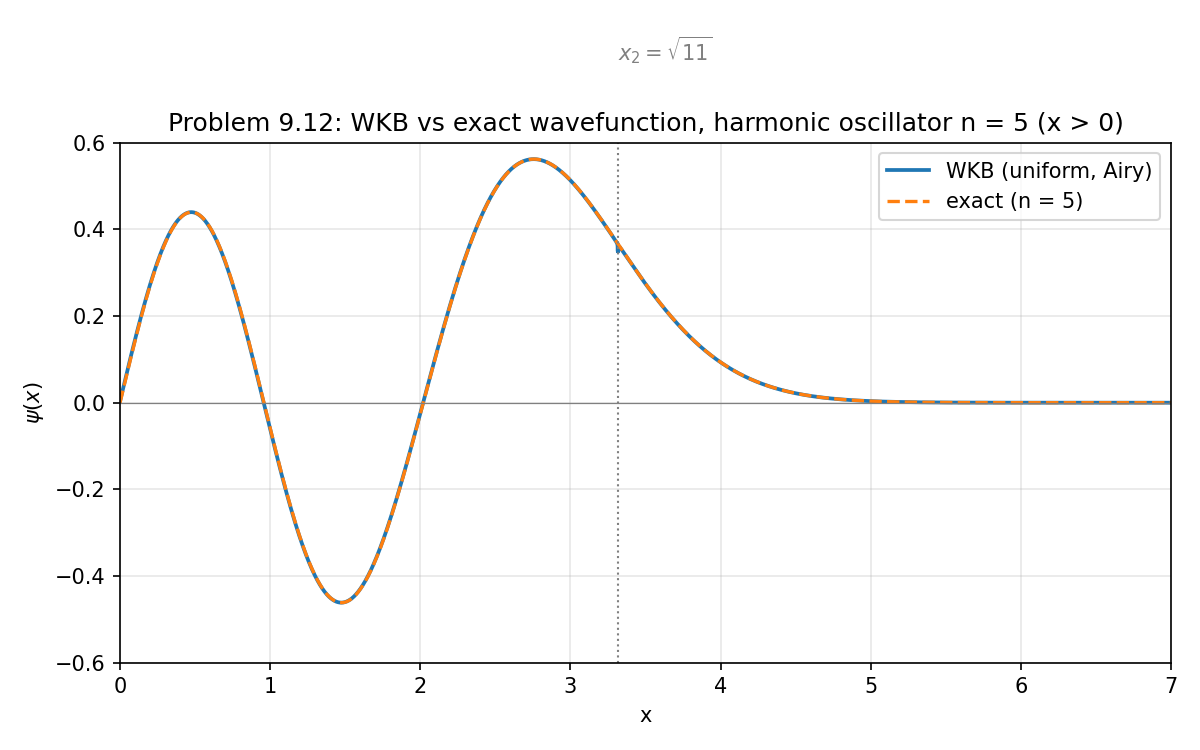
\includegraphics[width=0.8\textwidth,valign=t]{fig/prob9.12.png}

\subsection*{Sol. 13}
\begin{align*}
    2\int_0^{x_2}
    \sqrt{2m(E-\alpha x^\nu)}dx
    =(n-\frac{1}{2})\pi\hbar
\end{align*}
Let $y=(2m\alpha)^{1/\nu} x$
\begin{align*}
    2\frac{1}{(2m\alpha)^{1/\nu}}\int_0^{y_2}
    \sqrt{2mE - y^\nu}dy
    =(n-\frac{1}{2})\pi\hbar
\end{align*}
\begin{align*}
    \frac{2}{(2m\alpha)^{1/\nu}}
    \frac{(2mE)^{\frac{1}{\nu}(1+\frac{\nu}{2})}
    \Gamma(\frac{1}{\nu})
    \Gamma(\frac{3}{2})
    }
    {\nu\Gamma(\frac{1}{\nu}+\frac{3}{2})}
    =(n-\frac{1}{2})\pi\hbar
\end{align*}
\begin{align*}
    E_n
    =&
    \frac{1}{2m}
    \left[(n-\frac{1}{2})\pi\hbar
    \frac{(2m\alpha)^{1/\nu}}{2}
    \frac
    {\nu\Gamma(\frac{1}{\nu}+\frac{3}{2})}
    {
    \Gamma(\frac{1}{\nu})
    \frac{\sqrt{\pi}}{2}
    }\right]^{\frac{2\nu}{2+\nu}}\\
    =&
    \left[(n-\frac{1}{2})\sqrt{\pi}\hbar
    \alpha^{1/\nu}
    (2m)^{\frac{-1}{2}}
    \frac
    {\Gamma(\frac{1}{\nu}+\frac{3}{2})}
    {
    \Gamma(\frac{1}{\nu}+1)
    }\right]^{\frac{2\nu}{2+\nu}}\\
    =&
    \alpha
    \left[(n-\frac{1}{2})
    \hbar
    \sqrt{\frac{\pi}{2m\alpha}}
    \frac
    {\Gamma(\frac{1}{\nu}+\frac{3}{2})}
    {
    \Gamma(\frac{1}{\nu}+1)
    }\right]^{\frac{2\nu}{2+\nu}}
\end{align*}
For $\nu=2,$
\begin{align*}
    E_n = &
    \alpha
    \left[(n-\frac{1}{2})
    \hbar
    \sqrt{\frac{\pi}{2m\alpha}}
    \frac
    {\Gamma(2)}
    {
    \Gamma(\frac{3}{2})
    }\right]\\
    =&
    (n-\frac{1}{2})
    \hbar
    \sqrt{\frac{2\alpha}{m}}
\end{align*}

\subsection*{Sol. 14}
\begin{align*}
    (n-\frac{1}{2})\pi\hbar=&
    2\int_0^{x_2}\sqrt{2mE + 2\hbar^2a^2\operatorname{sech}^2(ax)}
    dx\\
    =&
    2\sqrt{2}\hbar a
    \int_0^{x_2}\sqrt{\frac{mE}{\hbar^2 a^2} + \operatorname{sech}^2(ax)}
    dx\\
    =&
    2\sqrt{2}\hbar a\left(\frac{\arctan\left(\frac{\sqrt{\frac{\hbar^2 a^2}{-mE}} \sinh\left(ax\right)}{\sqrt{\frac{\hbar^2 a^2}{-mE} - \cosh^{2}\left(ax\right)}}\right)}{a} - \frac{\arcsin\left(\frac{\sinh\left(ax\right)}{\sqrt{\frac{\hbar^2 a^2}{-mE} - 1}}\right)}{a \sqrt{\frac{\hbar^2 a^2}{-mE}}}\right)\bigg|^{x_2}_0\\
    =&
    2\sqrt{2}\hbar a\left[\frac{\pi/2}{a}-
    \frac{\pi/2}{a \sqrt{\frac{\hbar^2 a^2}{-mE}}}\right]
\end{align*}
Only $n=1$ is allowed,
\begin{align*}
    E=&\frac{a^2}{-2m}(\sqrt{2}\hbar -(1-\frac{1}{2})\hbar)^2\\
    =&-\left[\frac{9}{8}-\frac{1}{\sqrt{2}}\right]a^2\hbar^2/m,
\end{align*}
which yields the same answer as the exact case.

\subsection*{Sol. 15}
\begin{align*}
    (n-\frac{1}{4})\pi\hbar=&
    \int_0^{r_0}
    \sqrt{2mE-2mV_0\ln(r)-2mV_0\ln(a)}dr\\
    =&
    \sqrt{2mV_0}
    \int_0^{r_0}
    \sqrt{
    \frac{E - V_0\ln a}{V_0}
    -\ln r
    }dr\\
    =&
    \sqrt{2mV_0}
    \frac{\sqrt{\pi} \, \mathrm{e}^{\frac{E - V_0\ln a}{V_0}}}{2}
\end{align*}
\begin{align*}
    E_n =
    V_0\ln a+
    V_0
    \ln\left[2(n-\frac{1}{4})
    \frac{\sqrt{\pi}\hbar}{\sqrt{2mV_0}}\right]
\end{align*}
\begin{align*}
    E_{n+1}
    -E_n
    =
    V_0
    \ln\left[
    \frac{n+\frac{3}{4}}{n-\frac{1}{4}}
    \right]
\end{align*}

\subsection*{Sol. 16}
\begin{align*}
    (n'-\frac{1}{2})\pi\hbar=&\int_{r_1}^{r_2}
    \sqrt{2m(E+\frac{e^2}{4\pi\epsilon_0}\frac{1}{r}-\frac{\hbar^2}{2m}\frac{l(l+1)}{r^2})}dr\\
    =&
    \sqrt{-2mE}\int_{r_1}^{r_2}
    \frac{1}{r}
    \sqrt{-r^2-\frac{e^2}{4\pi\epsilon_0 E}r+
    \frac{\hbar^2}{2mE}l(l+1)}dr\\
    =&\sqrt{-2mE}
    \frac{\pi}{2}(\sqrt{r_2}-\sqrt{r_1})^2\\
    =&\sqrt{-2mE}
    \frac{\pi}{2}(-\frac{e^2}{4\pi\epsilon_0 E}-2\sqrt{\frac{\hbar^2l(l+1)}{-2mE}})\\
    =&
    \sqrt{2m}
    \frac{\pi}{2}(\frac{e^2}{4\pi\epsilon_0 \sqrt{-E}}-2\sqrt{\frac{\hbar^2l(l+1)}{2m}})
\end{align*}
\begin{align*}
    \left[\frac{1}{4\pi\epsilon_0}\frac{e^2}{\frac{2}{\sqrt{2m}}(n'-\frac{1}{2})\hbar+
    2\sqrt{\frac{\hbar^2l(l+1)}{2m}}}\right]^2
    =
    \frac{13.6 eV}
    {[(n'-\frac{1}{2})+
    \sqrt{l(l+1)}]^2}
    =-E_{n',l}
\end{align*}
\begin{align*}
    \frac{-13.6 eV}
    {[(n-l-\frac{1}{2})+
    \sqrt{l(l+1)}]^2}\approx&
    \frac{-13.6 eV}
    {[(n-l-\frac{1}{2})+
    l(1+\frac{1}{2}\frac{1}{l} -\frac{1}{8}\frac{1}{l^2})]^2}\\
    =&\frac{-13.6eV}{(n-\frac{1}{8l})^2},
\end{align*}
The WKB approximation gives an extra energy split in $l.$

\subsection*{Sol. 17}
\begin{enumerate}
    \item 
    Part i and part ii are shown as equation 9.47.
    Assume that 
    \begin{align*}
        \psi(x) = 
        \begin{cases}
        \frac{2D}{\sqrt{p(x)}}\sin\left[
        \frac{1}{\hbar}\int_{x}^{x_2}p(x')dx'+\frac{\pi}{4}
        \right],\;x_1<x<x_2
        \\
        \frac{1}{\sqrt{|p(x)|}}[Ae^{-\frac{1}{\hbar}\int_x^{x_1}|p(x')|dx'}+Be^{\frac{1}{\hbar}\int_x^{x_1}|p(x')|dx'}],\; 0<x<x_1
        \end{cases}
    \end{align*}
    The patching formula,
    \begin{align*}
        \psi(x)=a\operatorname{Ai}(\alpha(x-x_1)) + b \operatorname{Bi}(\alpha(x-x_1)).
    \end{align*}
    $$
    p(x)=\sqrt{2m(E-E-V'(x_1)(x-x_1))}=\hbar(-\alpha)^{3/2}\sqrt{x-x_1},
    $$
    where $\alpha=\left[2mV'(x_1)\right]^{1/3}.$

    \begin{align*}
        \frac{1}{\hbar}\int_x^{x_2}p(x')dx'=&
        \frac{1}{\hbar}\int_x^{x_1}p(x')dx'+\theta\\
    =&-(-\alpha)^{3/2}\frac{2}{3}(x-x_1)^{3/2}+\theta
    \end{align*}
    \begin{align*}
        \frac{1}{\hbar}\int_x^{x_1}|p(x')|dx'
    =(-\alpha)^{3/2}\frac{2}{3}(x_1-x)^{3/2}
    \end{align*}
    Thus,
    \begin{align*}
        \psi(x) \approx
        \begin{cases}
        \frac{2D}{\sqrt{\hbar}(-\alpha)^{3/4}(x-x_1)^{1/4}}
        \sin\left[
        \theta-(-\alpha)^{3/2}\frac{2}{3}(x-x_1)^{3/2}+\frac{\pi}{4}
        \right],\;x_1<x<x_2
        \\
        \frac{1}{\sqrt{\hbar}(-\alpha)^{3/4}(x_1-x)^{1/4}}
        [Ae^{-(-\alpha)^{3/2}\frac{2}{3}(x_1-x)^{3/2}}+
        Be^{(-\alpha)^{3/2}\frac{2}{3}(x_1-x)^{3/2}}],\; 0<x<x_1
        \end{cases}
    \end{align*}
    
    For $x>x_1,$ use the large negative approximation
    \begin{align*}
        \psi(x)=&\frac{a}{\sqrt{\pi}(-\alpha(x-x_1))^{1/4}}
        \sin\left[
        \frac{2}{3}(-\alpha(x-x_1)^{3/2})+\frac{\pi}{4}
        \right]\\
        &+ \frac{b}{\sqrt{\pi}(-\alpha(x-x_1))^{1/4}}
        \cos\left[
        \frac{2}{3}(-\alpha(x-x_1)^{3/2})+\frac{\pi}{4}
        \right]
    \end{align*}
    \begin{align*}
        \sin\left[
        \theta-(-\alpha)^{3/2}\frac{2}{3}(x-x_1)^{3/2}+\frac{\pi}{4}
        \right]
        =&-\sin\left[
        (-\alpha)^{3/2}\frac{2}{3}(x-x_1)^{3/2}+\frac{\pi}{4}-\frac{\pi}{2}-\theta
        \right]\\
        =&
        -\sin\left[
        \frac{2}{3}(-\alpha(x-x_1)^{3/2})+
        \frac{\pi}{4}
        \right]\cos(\frac{\pi}{2}+\theta)
        \\
        &+
        \cos\left[
        \frac{2}{3}(-\alpha(x-x_1)^{3/2})+\frac{\pi}{4}
        \right]
        \sin(\frac{\pi}{2}+\theta),
    \end{align*}
    \begin{align*}
        \frac{2D}{\sqrt{\hbar}(-\alpha)^{3/4}(x-x_1)^{1/4}}
        (-\cos(\pi/2+\theta))
        =\frac{a}{\sqrt{\pi}(-\alpha)^{1/4}(x-x_1)^{1/4}}
        \Rightarrow
        a = \frac{2D\sqrt{\pi}}{\sqrt{\hbar}(-\alpha)^{1/2}}\sin(\theta)
    \end{align*}
    \begin{align*}
        \frac{2D}{\sqrt{\hbar}(-\alpha)^{3/4}(x-x_1)^{1/4}}
        (\sin(\pi/2+\theta))
        =\frac{b}{\sqrt{\pi}(-\alpha)^{1/4}(x-x_1)^{1/4}}
        \Rightarrow
        b = \frac{2D\sqrt{\pi}}{\sqrt{\hbar}(-\alpha)^{1/2}}\cos(\theta)
    \end{align*}

    For $x<x_1,$ use the large approximation
    \begin{align*}
        \psi(x)=
        \frac{a}{2\sqrt{\pi}(\alpha(x-x_1))^{1/4}}e^{-\frac{2}{3}(\alpha(x-x_1))^{3/2}}+
        \frac{b}{\sqrt{\pi}(\alpha(x-x_1))^{1/4}}e^{\frac{2}{3}(\alpha(x-x_1))^{3/2}}
    \end{align*}
    \begin{align*}
        \frac{a}{2\sqrt{\pi}(\alpha(x-x_1))^{1/4}} = \frac{A}{\sqrt{\hbar}(-\alpha)^{3/4}(x_1-x)^{1/4}}
        \Rightarrow
        A =\frac{a\sqrt{\hbar}(-\alpha)^{1/2}}{2\sqrt{\pi}}
    \end{align*}
    \begin{align*}
        \frac{b}{\sqrt{\pi}(\alpha(x_1-x))^{1/4}} = \frac{B}{\sqrt{\hbar}(-\alpha)^{3/4}(x-x_1)^{1/4}}
        \Rightarrow 
        B = \frac{b\sqrt{\hbar}(-\alpha)^{1/2}}{\sqrt{\pi}}
    \end{align*}
    \begin{align*}
        A = D\sin\theta,\;
        B = 2D\cos\theta.
    \end{align*}
    Thus, for part iii
    \begin{align*}
        \psi(x)
        =\frac{D}{\sqrt{|p(x)|}}[\sin\theta e^{-\frac{1}{\hbar}\int_x^{x_1}|p(x')|dx'}+2\cos\theta e^{\frac{1}{\hbar}\int_x^{x_1}|p(x')|dx'}].
    \end{align*}
    \item 
    If $\psi$ is even.
    Since $p(x)$ is even, the numerator must be odd, thus its derivative must be 0 at $x=0,$ thus
    \begin{align*}
        2\cos\theta e^{\frac{1}{\hbar}\int_0^{x_1}|p(x')|dx'}
        \frac{1}{\hbar}p(0)
        -
        \sin\theta e^{-\frac{1}{\hbar}
        \int_0^{x_1}|p(x')|dx'}
        \frac{1}{\hbar}
        p(0)=0
    \end{align*}
    \begin{align*}
        2\cos\theta e^{\phi/2}
        -\sin\theta e^{-\phi/2}=0\Rightarrow
        \tan\theta = 2e^\phi.
    \end{align*}
    If $\psi$ is odd,
    \begin{align*}
        2\cos\theta e^{\frac{1}{\hbar}\int_0^{x_1}|p(x')|dx'}
        +
        \sin\theta e^{-\frac{1}{\hbar}
        \int_0^{x_1}|p(x')|dx'}=0
    \end{align*}
    \begin{align*}
        2\cos\theta e^{\phi/2}
        +\sin\theta e^{-\phi/2}=0\Rightarrow
        \tan\theta = -2e^\phi.
    \end{align*}
    \item 
    \begin{align*}
        \tan((n+\frac{1}{2})\pi+\epsilon)
        =-\cot \epsilon\approx -\frac{1}{\epsilon}
        =\pm 2e^\phi
        \Rightarrow
        \epsilon\approx \mp \frac{1}{2}e^{-\phi}
    \end{align*}
    \item 
    \begin{align*}
        \theta =&\frac{1}{\hbar}
        \int_{x_1}^{x_2}\sqrt{2m(E-\frac{1}{2}m\omega^2(x-a)^2)}dx\\
        =&
        \frac{1}{\hbar}
        \int_{x_1}^{x_2}\sqrt{-m^2\omega^2x^2+2m^2\omega^2ax+2mE-m^2\omega^2a^2}dx\\
        =&
        \frac{\pi}{\hbar}
        \frac{4(-m^2\omega^2)(2mE-m^2\omega^2a^2)-(2m^2\omega^2a)^2}{8(-m^2\omega^2)}
        \frac{1}{\sqrt{-(-m^2\omega^2)}}\\
        =&
        \frac{\pi E}{\hbar\omega}
    \end{align*}
    \begin{align*}
        (n+\frac{1}{2})\pi\mp \frac{1}{2}e^{-\phi}=\frac{\pi E}{\hbar\omega}
        \Rightarrow
        E_n^{\pm}=(n+\frac{1}{2})\hbar\omega \mp \frac{\hbar\omega}{2\pi}e^{-\phi}
    \end{align*}
    \item 
    \begin{align*}
        \Psi(x,t)=\frac{1}{\sqrt{2}}(\psi_n^+e^{-iE_n^+t/\hbar}
        +\psi_n^-e^{-iE_n^-t/\hbar})
    \end{align*}
    \begin{align*}
        \langle x\rangle
        =&
        \int 
        \frac{1}{\sqrt{2}}(\psi_n^+e^{iE_n^+t/\hbar}
        +\psi_n^-e^{iE_n^-t/\hbar})x
        \frac{1}{\sqrt{2}}(\psi_n^+e^{-iE_n^+t/\hbar}
        +\psi_n^-e^{-iE_n^-t/\hbar})dx\\
        =&
        \frac{1}{2}\langle x\rangle_+
        +\frac{1}{2}\langle x\rangle_-
        +
        \frac{1}{2}
        \int\psi_n^+\psi_n^-x[e^{i(E_n^+-E_n^-)t/\hbar}
        +e^{-i(E_n^+-E_n^-)t/\hbar}]dx\\
        =&
        \frac{1}{2}\langle x\rangle_+
        +\frac{1}{2}\langle x\rangle_-
        +
        \cos\frac{\omega}{\pi}e^{-\phi}t
        \int\psi_n^+\psi_n^-xdx
    \end{align*}
    The period is 
    $$
    \tau = \frac{2\pi^2}{\omega}e^{\phi}.
    $$
    \item 
    \begin{align*}
        \phi =& \frac{2}{\hbar}\int_0^{x_1}\sqrt{2m(\frac{1}{2}m\omega^2(x-a)^2-E)}dx\\
        =&\frac{2}{\hbar}
        \left[\frac{\sqrt{E} \sqrt{m} \left(x - a\right) \sqrt{\frac{m{\omega}^{2} \left(x - a\right)^{2} - 2E}{E}}}{2} - \frac{E \ln\left(\left|\sqrt{m{\omega}^{2} \left(x - a\right)^{2} - 2E} + \sqrt{m} \, {\omega} \left(x - a\right)\right|\right)}{\omega}
        \right]\bigg|^{a-\frac{\sqrt{2E}}{\omega\sqrt{m}}}_0\\
        =&
        \frac{2}{\hbar}
        \left[
        -\frac{E\ln|\sqrt{2E}|}{\omega}
        +\frac{a\sqrt{E} \sqrt{m}  \sqrt{\frac{m{\omega}^{2} 
        a^2 - 2E}{E}}}{2} + 
        \frac{E \ln\left(\left|\sqrt{m{\omega}^{2} a^2 - 2E} + \sqrt{m} \, {\omega} \left(- a\right)\right|\right)}{\omega}
        \right]\\
        =&
        \frac{2}{\hbar\omega}
        \left[
        \frac{a\omega}{2}\sqrt{m}\sqrt{m\omega^2a^2-2E}
        +E\ln\frac{\sqrt{m\omega^2a^2-2E}-a\omega\sqrt{m}}{\sqrt{2E}}
        \right]
    \end{align*}
    If $\frac{1}{2}m\omega^2 a^2\gg E,$ then 
    \begin{align*}
        \phi \approx 
        \frac{2}{\hbar\omega}
        \frac{a\omega}{2}
        \sqrt{m}\sqrt{m\omega^2a^2}
        =\frac{a^2}{\hbar}m\omega.
    \end{align*}
\end{enumerate}

\subsection*{Sol. 18}
\begin{enumerate}
    \item 
    $$
    E+V_0= \frac{\pi^2\hbar^2}{8ma^2}
    $$
    \item 
    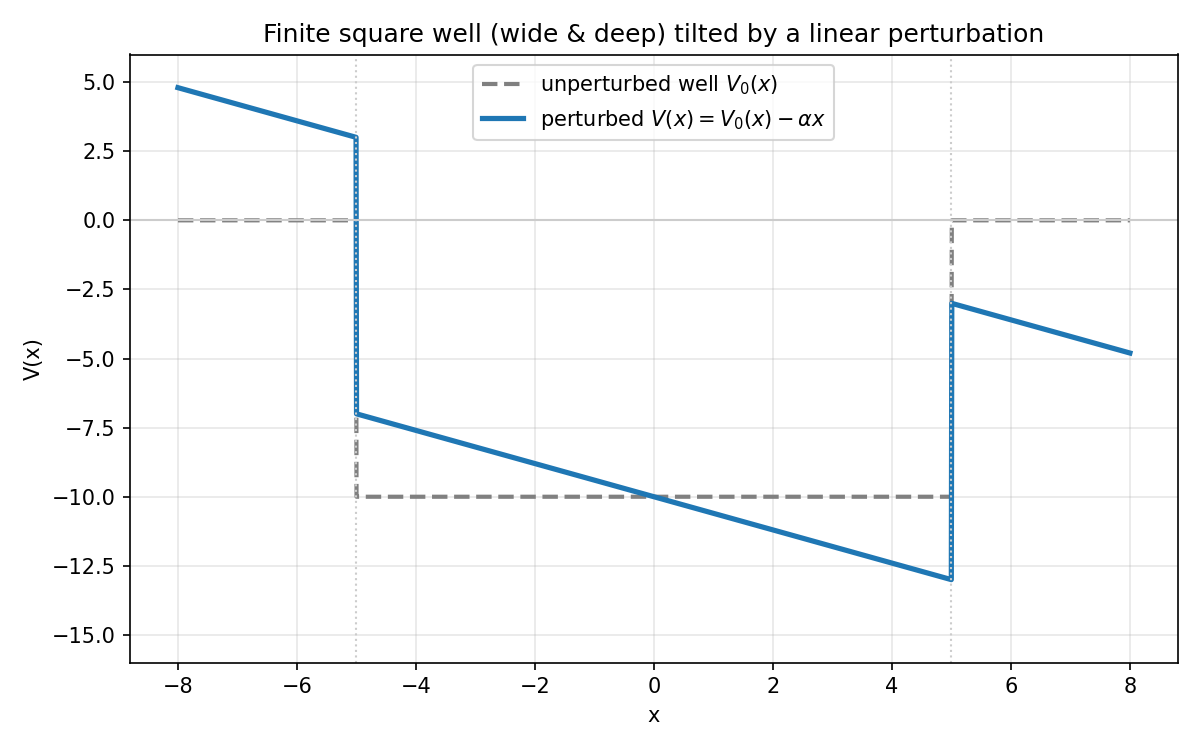
\includegraphics[width=0.8\textwidth,valign=t]{fig/sketch_tilted_well.png}
    \item 
    The barrier starts from $a$ to $\frac{1}{\alpha}\left[
    V_0-\frac{\pi^2\hbar^2}{8ma^2}
    \right].$
    \begin{align*}
        \gamma =& \frac{1}{\hbar}
        \int_a^{\frac{1}{\alpha}\left[
    V_0-\frac{\pi^2\hbar^2}{8ma^2}
    \right]}\sqrt{2m(-\alpha x +V_0-\frac{\pi^2\hbar^2}{8ma^2})}dx\\
    =&
    \frac{1}{\hbar}
    \frac{-2^{\frac{3}{2}} \sqrt{m} \left(-{\alpha}x - \frac{\pi^{2} h^{2}}{8a^{2} m} + V_{0}\right)^{\frac{3}{2}}}{3{\alpha}}
    \bigg|^{\frac{1}{\alpha}\left[
    V_0-\frac{\pi^2\hbar^2}{8ma^2}
    \right]}_a\\
    =&
     \frac{1}{\hbar}
    \frac{2^{\frac{3}{2}} \sqrt{m} \left(-{\alpha}a - \frac{\pi^{2} h^{2}}{8a^{2} m} + V_{0}\right)^{\frac{3}{2}}}{3{\alpha}}\\
    \approx &
     \frac{\sqrt{8mV_0^3}}{3\alpha\hbar}
    \end{align*}
    The kinetic energy is $\frac{\pi^2\hbar^2}{8ma^2},$ so the momentum is $\frac{\pi\hbar}{2a},$ thus 
    $$
    \tau = \frac{4a}{\frac{\pi\hbar}{2a}/m}e^{2\gamma}
    =\frac{8ma^2}{\pi\hbar}e^{2\gamma}.
    $$
    \item $$
    \gamma = 43640
    $$
    $$
    \tau\approx 10^{37882}yrs
    $$
    The age of the universe is $10^{10}yrs,$ so the tunneling in the Stark effect is not an issue.
    
    
\end{enumerate}

\subsection*{Sol. 19}
\begin{align*}
    \gamma = \frac{1}{\hbar}\int_0^{x_0}
    \sqrt{2m^2gx}dx
    =\frac{1}{\hbar}\sqrt{2m^2 g}\frac{2}{3}(\sqrt{R^2+(h/2)^2}-h/2)^{\frac{3}{2}}
\end{align*}
Estimate $R=3.3cm,$ $h=12.2cm,$ $m=380 g$ then $\gamma=8\times 10^{30}.$
$
v\approx 1.04\times10^{-10}m/s
$
$$
\tau \approx 20\times  e^{16\times 10^{30}} yrs.
$$

\subsection*{Sol. 20}
\begin{enumerate}
    \item 
    \begin{align*}
    Ae^{-ika}+Be^{ika}
    =\frac{1}{\sqrt{p(-a)}}
    [C_+e^{i\phi(-a)}+C_-e^{-i\phi(-a)}]
\end{align*}
\begin{align*}
   \frac{1}{\sqrt{p(a)}}
    [C_+e^{i\phi(a)}+C_-e^{-i\phi(a)}]
    =Ce^{ika}
\end{align*}
Since we assume that $V$ is analytic and vanishes when $|x|>a,$ $p'(\pm a)=0.$
\begin{align*}
    ikAe^{-ika}-ikBe^{ika}
    =&\frac{1}{p(-a)}
    [(i\phi'(-a)C_+e^{i\phi(-a)}-i\phi'(-a)C_-e^{-i\phi(-a)})\sqrt{p(-a)}]\\
    \Rightarrow
    kAe^{-ika}-kBe^{ika}=&\frac{1}{\hbar}(C_+e^{i\phi(a)}-C_-e^{-i\phi(a)})\sqrt{p(a)}
\end{align*}
\begin{align*}
    ikCe^{ika}
    =&\frac{1}{p(a)}
    [(i\phi'(a)C_+e^{i\phi(a)}-i\phi'(a)C_-e^{-i\phi(a)})\sqrt{p(a)}]\\
    \Rightarrow 
    kCe^{ika}=&\frac{1}{\hbar}(C_+e^{i\phi(a)}-C_-e^{-i\phi(a)})\sqrt{p(a)}
\end{align*}

Therefore
\begin{align*}
     Ae^{-ika}+Be^{ika}=Ce^{ika},\; Ae^{-ika}-Be^{ika} = Ce^{ika}
\end{align*}
\begin{align*}
    A = \frac{1}{2}Ce^{ika},\;
    B = 0.
\end{align*}
\item 
\begin{align*}
    p(iy)=&\sqrt{2m(E-V_0\operatorname{sech}^2(iy/a))}\\
    =&\sqrt{2m(E-\frac{4V_0}{e^{2iy/a}+e^{-2iy/a}+2})}\\
    =&\sqrt{2m(E-\frac{4V_0}{2\cos(2y/a)+2})}
\end{align*}
$$
\cos(2y_0/a)=\frac{2V_0}{E}-1
$$
$$
\tan^2(y_0/a)=\frac{1-\frac{2V_0}{E}+1}{1+\frac{2V_0}{E}-1}
=\frac{E-V_0}{V_0}
$$
\begin{align*}
    \lambda=&\frac{2}{\hbar}
    \int_0^{y_0}
    \sqrt{2mE-\frac{4mV_0}{\cos(2y/a)+1}}dy\\
    =&
    \frac{2}{\hbar}\sqrt{4mV_0}
    \left[
    \sqrt{\frac{E}{2V_0}} \, a \arctan\left(\frac{\sqrt{2} \sqrt{\frac{E}{2V_0}} \tan\left(\frac{y}{a}\right)}{\sqrt{-\tan^{2}\left(\frac{y}{a}\right) + 2\frac{E}{2V_0} - 1}}\right) - \frac{a \arcsin\left(\frac{\tan\left(\frac{y}{a}\right)}{\sqrt{2\frac{E}{2V_0} - 1}}\right)}{\sqrt{2}}
    \right]\bigg|^{y_0}_0\\
    =&
    \frac{2}{\hbar}\sqrt{4mV_0}
    \left[
    \sqrt{\frac{E}{2V_0}} \, a \frac{\pi}{2} - \frac{a}{\sqrt{2}}\frac{\pi}{2}
    \right]\\
    =&\frac{\pi a}{\hbar}(\sqrt{2mE}-\sqrt{2mV_0})
\end{align*}
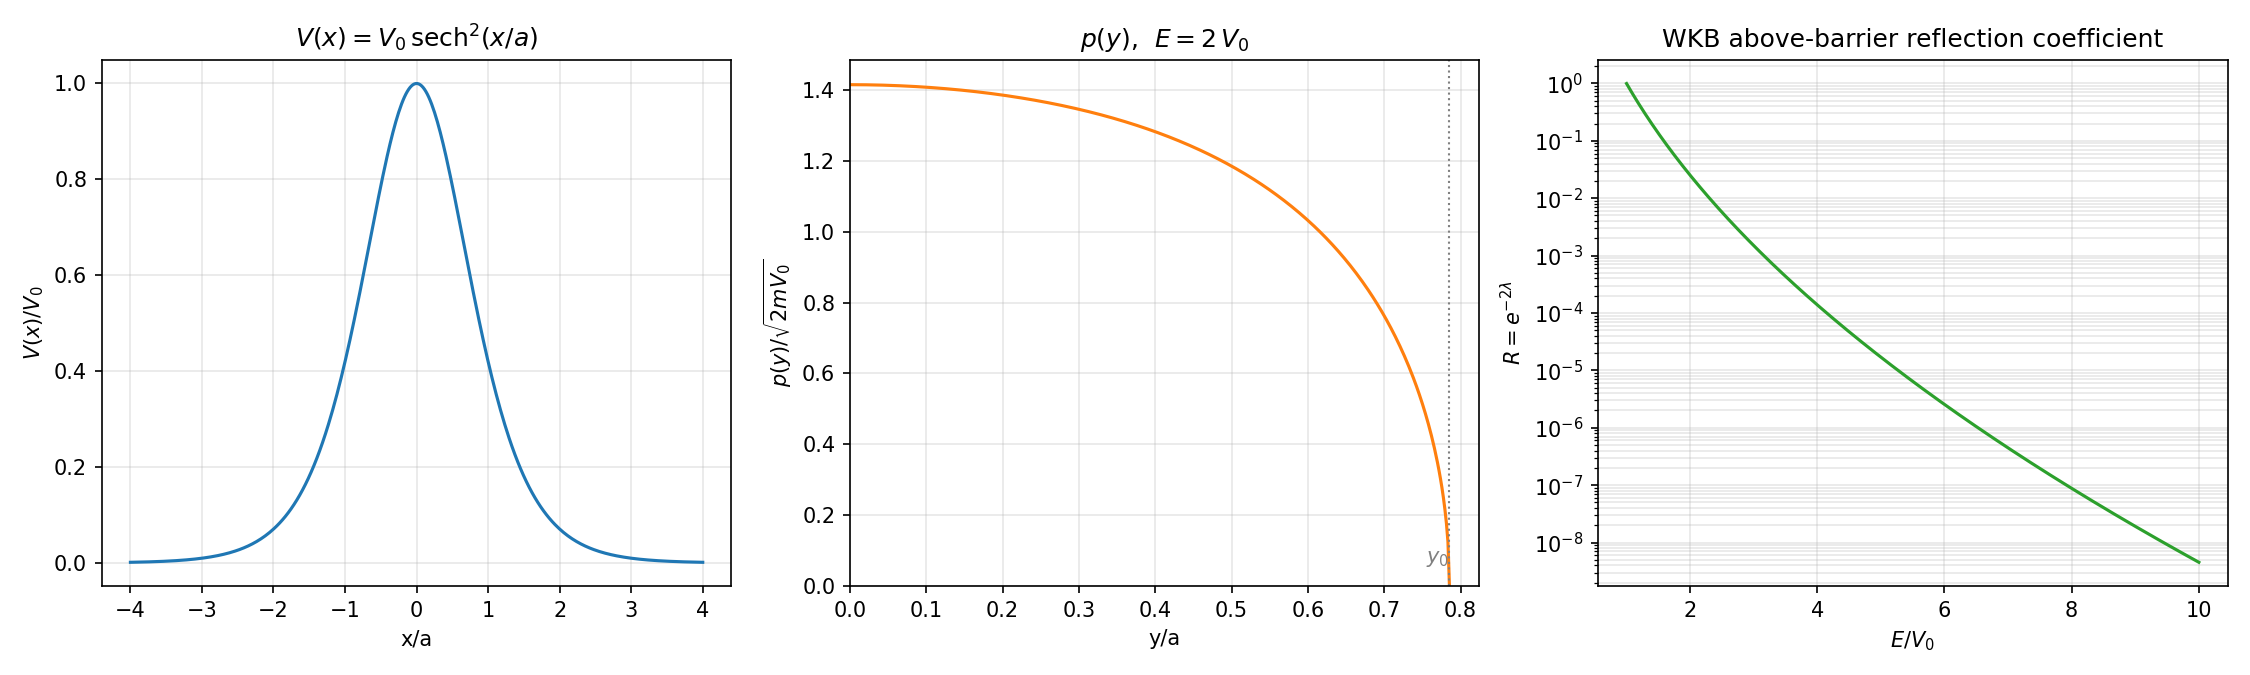
\includegraphics[width=0.8\textwidth,valign=t]{fig/prob9.20.png}
\item 
\begin{align*}
    \lambda =& \frac{2}{\hbar}
    \int_0^{y_0}
    \sqrt{2m(E - \frac{V_0}{1+(iy/a)^2})}dy\\
    =&
     \frac{2}{\hbar}
    \int_0^{y_0}
    \sqrt{2m(E - \frac{V_0}{1-(y/a)^2})}dy\\
    =&
    (2a\sqrt{2mE}/\hbar) [ E(k0) - (V_0/E)K(k_0) ],
\end{align*}
where $k_0 = \sqrt(1-V_0/E),$ and 
$K, E$ = complete elliptic integrals of the 1st/2nd kind, modulus k.

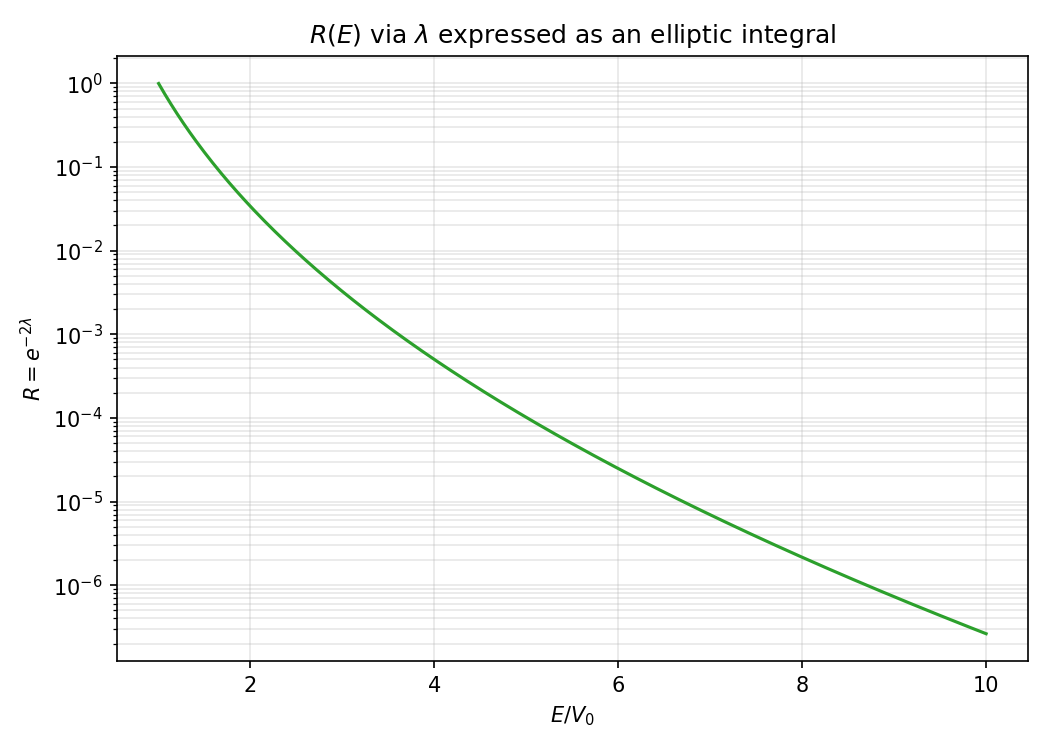
\includegraphics[width=0.8\textwidth,valign=t]{fig/prob9.20d.png}

\end{enumerate}

\subsection*{Sol. 21}
\begin{align*}
    \log_{10}\tau\ln2 
    = & \log_{10} \ln 2 +  \log_{10} \frac{2r_1}{v}e^{2\gamma}\\
    =&\log_{10} \ln 2 +  2(K_1\frac{Z}{\sqrt{E}}-K_2\sqrt{Z r_1})\log_{10}e+\log_{10} \frac{2r_1}{v}.
\end{align*}
The slope would be $-2K_1 Z\log_{10}e= -150.$ From $E = 5MeV$ to $6MeV,$ $\frac{-1}{\sqrt{E}}$ changes about $0.040MeV^{-1/2},$ thus the value of logarithm half life should decrease by $5.9,$ which matches the slope of the figure.

\section{Scattering}
\subsection*{Sol. 1}
\begin{enumerate}
    \item
          Since the magnitude of momentum is unchanged after the scattering,
          $$
              \Delta p = 2mv_0\sin\theta/2.
          $$
          Only the impulse component along the symmetry axis of the hyperbola will produce a net momentum change. Therefore,
          \begin{align*}
              \Delta p =
              \frac{q_1q_2}{4\pi\epsilon_0}
              \int \frac{\cos\alpha}{r^2}dt,
          \end{align*}
          where $\alpha$ is the angle relative to the symmetry plane, with orientation.
          Using the conservation of the angular momentum,
          \begin{align*}
              L = mv_0 b = mr^2\frac{d\alpha}{dt}.
          \end{align*}
          \begin{align*}
              2mv_0\sin\theta/2 & =
              \frac{q_1q_2}{4\pi\epsilon_0}
              \int \frac{\cos\alpha}{r^2}dt \\
                                & =
              \frac{q_1q_2}{4\pi\epsilon_0}
              \int_{\frac{-\pi}{2}+\frac{\theta}{2}}^{\frac{\pi}{2}-\frac{\theta}{2}} \frac{\cos\alpha}{r^2}\frac{r^2}{v_0 b}d\alpha \\
                                & =
              \frac{q_1q_2}{4\pi\epsilon_0}
              \frac{1}{v_0 b}
              \left[\sin\left(\frac{\pi}{2}-\frac{\theta}{2}\right)
                  -\sin\left(-\frac{\pi}{2}+\frac{\theta}{2}\right)
                  \right] \\
                                & =
              \frac{q_1q_2}{4\pi\epsilon_0}
              \frac{1}{v_0 b}2\cos(\theta/2).
          \end{align*}
          Thus
          \begin{align*}
              b & =\frac{q_1q_2}{4\pi\epsilon_0}
              \frac{1}{mv^2_0}\cot(\theta/2) \\
                & =
              \frac{q_1q_2}{8\pi\epsilon_0E}
              \cot(\theta/2).
          \end{align*}
    \item
          \begin{align*}
              D(\theta) & =
              \frac{q_1q_2}{8\pi\epsilon_0E}
              \cot(\theta/2)\frac{1}{2\sin(\theta/2)\cos(\theta/2)}
              \frac{q_1q_2}{8\pi\epsilon_0E}
              \csc^2(\theta/2)\frac{1}{2} \\
                        & =\left[
                               \frac{q_1q_2}{16\pi\epsilon_0 E\sin^2(\theta/2)}
                               \right]^2
          \end{align*}
    \item
          \begin{align*}
              \sigma & =
              \int \left[
                       \frac{q_1q_2}{16\pi\epsilon_0 E\sin^2(\theta/2)}
                       \right]^2\sin\theta d\theta d\phi \\
                     & =
              \left[
                  \frac{q_1q_2}{16\pi\epsilon_0 E}
                  \right]^22\pi
              (-\frac{2}{\sin^{2}\left(\frac{\theta}{2}\right)})\bigg|^\pi_0=\infty
          \end{align*}

\end{enumerate}
\subsection*{Sol. 2}
Two dim:
$$
    \psi(r,\theta) \approx A\left[
        e^{ikx}+f(\theta)\frac{e^{ikr}}{\sqrt{r}}
        \right]
$$
One dim:
$$
    \psi(x) \approx A\left[
        e^{ikx}+f(\frac{x}{|x|})e^{-ikx}
        \right]
$$

\subsection*{Sol. 3}
\begin{align*}
    \sum_{l=0}^\infty
    i^l(2l+1)[j_l(ka)+ika_lh_l^{(1)}(ka)]P_l(\cos\theta )=0
\end{align*}
\begin{align*}
    0 & =\int_0^{\pi}
    \sum_{l=0}^\infty
    i^l(2l+1)[j_l(ka)+ika_lh_l^{(1)}(ka)]P_l(\cos\theta )
    P_{l'}(\cos\theta)
    \sin\theta
    d\theta \\
      & =
    i^l[j_l(ka)+ika_lh_l^{(1)}(ka)]
\end{align*}
\begin{align*}
    [j_l(ka)+ika_lh_l^{(1)}(ka)]=0
    \Rightarrow
    a_l = -\frac{j_l(ka)}{ikh_l^{(1)}(ka)}
    =i\frac{j_l(ka)}{kh_l^{(1)}(ka)}.
\end{align*}
\subsection*{Sol. 4}
Keeping only the $l=0$ term, the exterior wavefunction is
\begin{align*}
    \psi(r) & =
    A[j_0(kr) + ika_0h_0^{(1)}(kr)]P_0(\cos\theta) \\
            & =
    A[\frac{\sin kr}{kr} + a_0\frac{e^{ikr}}{r}]
\end{align*}
Fo the internal region
\begin{align*}
    \psi(r) = Cj_0(kr) + Dn_l(kr) = C\frac{\sin kr}{kr}.
\end{align*}
$\psi$ should be continuous at $r=a$:
\begin{align*}
    C\frac{\sin ka}{ka} =
    A[\frac{\sin ka}{ka} + a_0\frac{e^{ika}}{a}]
\end{align*}
$\psi'$ at $r=a$:
\begin{align*}
    -\frac{\hbar^2}{2m}
    \int_{a-\epsilon}^{a+\epsilon}
    \frac{d^2u}{dr^2}
    dr
    +
    \int_{a-\epsilon}^{a+\epsilon}
    (V(r) + \frac{\hbar^2}{2m}\frac{l(l+1)}{r^2})udr
    =
    E\int_{a-\epsilon}^{a+\epsilon}udr
\end{align*}
\begin{align*}
    \frac{du}{dr}\bigg|^{a+\epsilon}_{a-\epsilon}
     & =\frac{2m}{\hbar^2}\int_{a-\epsilon}^{a+\epsilon}V(r)udr \\
     & =\frac{2m}{\hbar^2}\alpha u(a)
\end{align*}
\begin{align*}
    A[\cos ka + a_0ike^{ika}] -
    C\cos ka = \frac{2m}{\hbar^2}\alpha
    C\frac{\sin ka}{k}
\end{align*}
Therefore,
\begin{align*}
    \frac{\sin ka}{ka}(\cos ka + a_0 ik e^{ika}) =
    [\frac{\sin ka}{ka} + a_0\frac{e^{ika}}{a}]
    (2m\alpha/\hbar^2 \sin (ka)/k+\cos ka)
\end{align*}
\begin{align*}
    a_0 & = \frac{\frac{\sin ka}{ka}(2m\alpha/\hbar^2 \sin (ka)/k+\cos ka)-\frac{\sin ka}{ka}\cos ka }
            {\frac{\sin ka}{ka} ike^{ika}-\frac{e^{ika}}{a}(2m\alpha/\hbar^2 \sin (ka)/k+\cos ka)} \\
        & =
    \frac{(2m\alpha/\hbar^2 a+1)-1 }
    {ike^{ika}-\frac{e^{ika}}{a}(2m\alpha/\hbar^2 a+1)} \\
        & =
    \frac{a\beta}{-(\beta+1)}
\end{align*}
\begin{align*}
    \sigma = 4\pi \frac{a^2\beta^2}{(\beta+1)^2}.
\end{align*}

\subsection*{Sol. 5}
\begin{enumerate}
    \item
          For $x<-a$,
          $$
              \psi(x) = Ae^{ik x} + Be^{-ikx}
          $$
          For $-a<x<0$,
          $$
              \psi(x) = Ce^{\kappa x}+De^{-\kappa x}
          $$
          $\psi$ has to vanish at $x=0$,
          $$
              C+D=0,
          $$
          continuous at $x=-a$,
          $$
              Ce^{-a\kappa }+De^{ a\kappa }
              =2D\sinh(a\kappa)
              =
              Ae^{-aik } + Be^{aik}
          $$
          and derivative continuous
          $$
              \kappa Ce^{-a\kappa }-\kappa De^{\kappa a}
              =-2\kappa D\cosh(\kappa a)
              =ikAe^{-aik } -ik Be^{aik}.
          $$

          \begin{align*}
              B & =\frac{\begin{vmatrix}
                           2\sinh(a\kappa)        & Ae^{-aik}   \\
                           -2\kappa\cosh(a\kappa) & ikAe^{-aik} \\
                       \end{vmatrix}}{\begin{vmatrix}
                           2\sinh(a\kappa)        & - e^{aik} \\
                           -2\kappa\cosh(a\kappa) & ike^{aik} \\
                       \end{vmatrix}} \\
                & =\frac{2ikAe^{-aik}\sinh(a\kappa)+2\kappa\cosh(a\kappa)Ae^{-aik}}
                   {ik2e^{aik}\sinh(a\kappa)-2\kappa e^{aik}\cosh(a\kappa)} \\
                & =Ae^{-2ika}
              \left[
                  \frac{k-i\kappa\coth(\kappa a)}{k+i\kappa\coth(\kappa a)}
                  \right]
          \end{align*}
    \item
          \begin{align*}
              |B| = |A| |e^{-2ika}| |\frac{k-i\kappa\coth(\kappa a)}{k+i\kappa\coth(\kappa a)}| = |A|
          \end{align*}
    \item If $V_0\gg E$, $\kappa = \frac{\sqrt{2mV_0}}{\hbar}$,
          \begin{align*}
              \frac{k-i\kappa\coth(\kappa a)}{k+i\kappa\coth(\kappa a)}
              =\frac{\sqrt{2mE}-i\sqrt{2mV_0}\coth(\kappa a)}
               {\sqrt{2mE}+i\sqrt{2mV_0}\coth(\kappa a)}
              =-1
          \end{align*}
          \begin{align*}
              \psi(x) = Ae^{ikx} - Ae^{-2ika}e^{-ikx}\Rightarrow
              \delta = -ka.
          \end{align*}
\end{enumerate}
\subsection*{Sol. 6}
\begin{align*}
    a_l = i\frac{j_l(ka)}{kh_l^{(1)}(ka)} = \frac{1}{2ik}(e^{2i\delta_l}-1)
\end{align*}
\begin{align*}
    \delta_l & =\frac{-i}{2}\ln(-2k\frac{j_l(ka)}{kh_l^{(1)}(ka)}+1) \\
             & =
    \frac{-i}{2}\ln(\frac{-j_l(ka)+in_l(ka)}{j_l(ka)+in_l(ka))}) \\
             & =\arctan(\frac{j_l(ka)}{n_l(ka)})
\end{align*}
\subsection*{Sol. 7}
For $l=0$,
\begin{align*}
    u(r) = C\sin(kr), \; 0<r<a,
\end{align*}
\begin{align*}
    u(r) =  Ae^{-ikr}+ Be^{ikr}, \; r>a.
\end{align*}
Continuous at $r=a$,
\begin{align*}
    C\sin(ka) = Ae^{-ika}+ Be^{ika}
\end{align*}
The derivative must satisfy
\begin{align*}
    \frac{du}{dr}\bigg|^{a+\epsilon}_{a-\epsilon}
    =\frac{2m}{\hbar^2}\alpha u(a)
\end{align*}
\begin{align*}
    -ikAe^{-ika} + ikBe^{ika} - Ck\cos(ka) = \frac{2m}{\hbar^2}\alpha C\sin(ka)
\end{align*}
\begin{align*}
    B & = \frac{{\begin{vmatrix}
                      Ae^{-ika}   & \sin(ka)                                    \\
                      ikAe^{-ika} & -k\cos(ka)-\frac{2m\alpha}{\hbar^2}\sin(ka)
                  \end{vmatrix}}}
          {\begin{vmatrix}
                  -e^{ika}  & \sin(ka)                                    \\
                  ike^{ika} & -k\cos(ka)-\frac{2m\alpha}{\hbar^2}\sin(ka)
              \end{vmatrix}} \\
      & =\frac{-Ae^{-ika}k\cos(ka)-\frac{2m\alpha}{\hbar^2}Ae^{-ika}\sin(ka)-ikAe^{-ika}\sin(ka)}
         {e^{ika}k\cos(ka)+\frac{2m\alpha}{\hbar^2}e^{ika}\sin(ka)-ike^{ika}\sin(ka)} \\
      & =-A
    \frac{(\cos(ka)-i\sin(ka))(ka\cos(ka)+\beta \sin(ka)+ika\sin(ka))}
    {(\cos(ka)+i\sin(ka))(ka\cos(ka)+\beta \sin(ka)-ika\sin(ka))} \\
      & =-A
    \frac{ka+\beta \cos(ka)\sin(ka)
        -i\beta\sin^2(ka)}
    {ka+\beta \cos(ka)\sin(ka)
        +i\beta\sin^2(ka)}=-Ae^{2i\delta}
\end{align*}
\begin{align*}
    \delta & = \frac{1}{2i}
    \log\left[
            \frac{ka+\beta \cos(ka)\sin(ka)
                -i\beta\sin^2(ka)}
            {ka+\beta \cos(ka)\sin(ka)
                +i\beta\sin^2(ka)}\right] \\
           & =-\operatorname{arccot}
    \left[
        \frac{ka+\beta\cos(ka)\sin(ka)}{\beta\sin^2(ka)}
        \right] \\
           & =
    -\operatorname{arccot}
    \left[\cot(ka) +
        \frac{ka}{\beta\sin^2(ka)}
        \right].
\end{align*}

\subsection*{Sol. 8}
\begin{align*}
    (\nabla^2 + k^2)(-\frac{e^{ikr}}{4\pi r})
     & =-(\nabla^2e^{ikr})\frac{1}{4\pi r}
    -2(\nabla e^{ikr})(\nabla\frac{1}{4\pi r})
    -e^{ikr}(\nabla^2\frac{1}{4\pi r})
    -k^2\frac{e^{ikr}}{4\pi r} \\
     & =-(ik\frac{2}{r}e^{ikr} - k^2e^{ikr} )\frac{1}{4\pi r}
    -2(ike^{ikr})(\frac{-1}{4\pi r^2})
    +e^{ikr}\delta^3(\bm r)-k^2\frac{e^{ikr}}{4\pi r} \\
     & =e^{ikr}\delta^3(\bm r) \\
     & =\delta^3(\bm r)
\end{align*}

\subsection*{Sol. 9}
$$
    k = i\sqrt{-2mE_1}/\hbar
    = \frac{i}{a}
$$

\begin{align*}
     & -\frac{m}{2\pi\hbar^2}
    \int \frac{e^{-|\bm r-\bm r_0|/a}}{|\bm r - \bm r_0|}\frac{-e^2}{4\pi\epsilon_0 |\bm r_0|}\frac{1}{\sqrt{\pi a^3}}
    e^{-|\bm r_0|/a}d\bm r_0 \\
     & =
    \frac{1}{a}
    \frac{1}{\sqrt{\pi a^3}}
    \int \frac{e^{-\sqrt{r^2+r_0^2-2rr_0\cos\theta }/a}}{\sqrt{r^2+r_0^2-2rr_0\cos\theta }}
    \frac{1}{r_0}
    e^{-r_0/a}r_0^2\sin\theta dr_0d\theta \\
     & =
    \frac{1}{\sqrt{\pi a^3}}
    \frac{-1}{r}
    \left[
        \int_0^{r}
        e^{-r_0/a}
        (e^{-(r+r_0)/a}
        -
        e^{-(r-r_0)/a}
        )
        dr_0
        +\int_r^\infty
        e^{-r_0/a}
        (e^{-(r+r_0)/a}
        -
        e^{-(r_0-r)/a}
        )
        dr_0
        \right] \\
     & =
    \frac{1}{\sqrt{\pi a^3}}
    \frac{-1}{r}
    \left[
        -\frac{\mathrm{e}^{-\frac{3r}{a}} \left(\left(2r - a\right) \mathrm{e}^{\frac{2r}{a}} + a\right)}{2}
        -\frac{a\mathrm{e}^{-\frac{3r}{a}} \left(\mathrm{e}^{\frac{2r}{a}} - 1\right)}{2}
        \right] \\
     & =
    \frac{1}{\sqrt{\pi a^3}}e^{-r/a}
\end{align*}

\subsection*{Sol. 10}
\begin{align*}
    f(\theta)
     & =-\frac{2m}{\hbar^2\kappa}
    \int_0^a
    rV_0\sin(\kappa r)dr \\
     & =
    -\frac{2m}{\hbar^2\kappa}
    \frac{V_{0} \left(\sin\left(a{\kappa}\right) - a{\kappa} \cos\left(a{\kappa}\right)\right)}{{\kappa}^{2}}
\end{align*}
For low energy scattering $ka\ll 1$,
$$
    \sin(a\kappa) - a\kappa\cos(a\kappa)
    \approx (a\kappa) - (a\kappa )^3/3!
    -(a\kappa)[1 - (a\kappa)^2/2!]
    =\frac{(a\kappa)^3}{3}
$$
\begin{align*}
    f(\theta) \approx &
    -\frac{2m}{\hbar^2\kappa^3}
    V_0
    \frac{(a\kappa)^3}{3} \\
                      & =-
    \frac{2ma^3}{3\hbar^2}
    V_0
\end{align*}

\subsection*{Sol. 11}
\begin{align*}
    -\frac{2m\beta}{\hbar^2\kappa}
    \int_0^\infty
    e^{-\mu r}\sin(\kappa r)dr
    =
    -\frac{2m\beta}{\hbar^2\kappa}\frac{\kappa}{\mu^2+\kappa^2}
    =-\frac{2m\beta}{\hbar^2(\mu^2+\kappa^2)}
\end{align*}

\subsection*{Sol. 12}
\begin{align*}
    D(\theta) =
    \frac{4m^2\beta^2}{\hbar^4(\mu^2+\kappa^2)^2}
\end{align*}
\begin{align*}
    \sigma & =
    2\pi\int_0^\pi
    \frac{4m^2\beta^2}{\hbar^4(\mu^2+4k^2\sin^2(\theta/2))^2}\sin\theta d\theta \\
           & =\frac{16\pi m^{2} {\beta}^{2}}{\hbar^{4} {\mu}^{2} \left({\mu}^{2} + 4k^{2}\right)} \\
           & =
    \frac{16\pi m^{2} {\beta}^{2}}{ \hbar^{4} {\mu}^{4} +
        \hbar^{2} {\mu}^{2}8mE}
\end{align*}

\subsection*{Sol. 13}
\begin{enumerate}
    \item \begin{align*}
              f(\theta)
               & =
              -\frac{m}{2\pi\hbar^2}
              \int\alpha\delta(|\bm r|-a)
              d\bm r \\
               & =
              -\frac{m}{2\pi\hbar^2}\alpha
              \int\delta(r-a)
              r^2\sin\theta drd\theta \\
               & =-\frac{2m\alpha  a^2}{\hbar^2}
          \end{align*}
          \begin{align*}
              D(\theta) = \frac{4m^2\alpha^2 a^4}{\hbar^4}
          \end{align*}
          \begin{align*}
              \sigma = \frac{16\pi m^2\alpha^2 a^4}{\hbar^4}
          \end{align*}
    \item
          \begin{align*}
              f(\theta) & =
              -\frac{2m}{\hbar^2\kappa}
              \int_0^\infty r\alpha \delta(r-a)\sin(\kappa r)dr \\
                        & =
              -\frac{2m}{\hbar^2\kappa}
              a\alpha \sin(\kappa a)
          \end{align*}
          Assume that $ka\ll 1$,
          \begin{align*}
              -\frac{2m}{\hbar^2\kappa}
              a\alpha \sin(\kappa a)
              \approx
              -\frac{2ma^2\alpha}{\hbar^2}.
          \end{align*}
          By 10.4,
          \begin{align*}
              -\frac{a\beta}{\beta+1}
              \approx
              -a\beta
              =-\frac{2ma^2\alpha}{\hbar^2}.
          \end{align*}
\end{enumerate}

\subsection*{Sol. 14}
\begin{align*}
    I & =\frac{q_1q_2}{4\pi\epsilon_0}\int
    \frac{1}{r^2}\sin\theta dt \\
      & =
    \frac{q_1q_2}{4\pi\epsilon_0}
    \int_{-\frac{\pi}{2}+\frac{\theta' }{2}}^{\frac{\pi}{2}-\frac{\theta' }{2}}
    \frac{1}{r^2}\sin(
    \frac{\pi-\theta'}{2}
    -\alpha + \theta '
    ) \frac{r^2}{v_0 b}d\alpha \\
      & =
    -\frac{q_1q_2}{4\pi\epsilon_0}
    \frac{1}{v_0 b}
    \sin(\frac{\theta'}{2}-\alpha)\bigg|^{\frac{\pi}{2}-\frac{\theta' }{2}}
                                        _{-\frac{\pi}{2}+\frac{\theta' }{2}} \\
      & =
    \frac{q_1q_2}{4\pi\epsilon_0}
    \frac{1}{v_0 b}(\cos\theta'+1)
    \approx\frac{q_1q_2}{2\pi\epsilon_0}
    \frac{1}{v_0 b}
\end{align*}
\begin{align*}
    \theta ' = \arctan\frac{\frac{q_1q_2}{2\pi\epsilon_0}
                          \frac{1}{v_0 b}}{mv_0}
    \approx \frac{q_1q_2}{4\pi\epsilon_0 bE}
\end{align*}

When $\theta'$ is small,
\begin{align*}
    b = \frac{q_1q_2}{8\pi\epsilon_0 E}\cot\frac{\theta }{2}
    \approx
    \frac{q_1q_2}{8\pi\epsilon_0 E}\frac{2}{\theta'}
    \Rightarrow \theta'
    =\frac{q_1q_2}{4\pi\epsilon_0 bE}
\end{align*}

\subsection*{Sol. 15}
\begin{align*}
    \psi(\bm r) & = \psi_0(\bm r) + \int g(\bm r -\bm r_0)V(\bm r_0)\psi(\bm r_0)d\bm r_0 \\
                & =
    \psi_0(\bm r) + \int g(\bm r -\bm r_0)V(\bm r_0)
    \left[
        \psi_0(\bm r_0) +
        \int g(\bm r_0 -\bm r_1)V(\bm r_1)\psi(\bm r_1)d\bm r_1
        \right]
    d\bm r_0 \\
    \approx     &
    Ae^{ikz}-\frac{m}{2\pi\hbar^2}
    \int\frac{e^{ik|\bm r-\bm r_0|}}{|\bm r - \bm r_0|}
    V(\bm r_0)\psi_0(\bm r_0)d\bm r_0
    +\frac{m^2}{4\pi^2\hbar^4}\int
    \frac{e^{ik|\bm r-\bm r_0|}}{|\bm r - \bm r_0|}
    \frac{e^{ik|\bm r_0-\bm r_1|}}{|\bm r_0 - \bm r_1|}
    V(\bm r_0)V(\bm r_1)\psi_0(\bm r_1)d\bm r_0d\bm r_1 \\
                & =
    Ae^{ikz}-\frac{m}{2\pi\hbar^2}
    \frac{e^{ikr}}{r}
    \int e^{-i\bm k \cdot \bm r_0}
    V(\bm r_0)\psi_0(\bm r_0)d\bm r_0
    +\frac{m^2}{4\pi^2\hbar^4}\frac{e^{ikr}}{r}
    \int e^{-i\bm k \cdot \bm r_0}
    \frac{e^{ik|\bm r_0-\bm r_1|}}{|\bm r_0 - \bm r_1|}
    V(\bm r_0)V(\bm r_1)\psi_0(\bm r_1)d\bm r_0d\bm r_1
\end{align*}
\begin{align*}
    f(\theta) & =
    -\frac{m}{2\pi\hbar^2A}
    \int e^{-i\bm k \cdot \bm r_0}
    V(\bm r_0)\psi_0(\bm r_0)d\bm r_0
    +\frac{m^2}{4\pi^2\hbar^4A}
    \int e^{-i\bm k \cdot \bm r_0}
    \frac{e^{ik|\bm r_0-\bm r_1|}}{|\bm r_0 - \bm r_1|}
    V(\bm r_0)V(\bm r_1)\psi_0(\bm r_1)d\bm r_1d\bm r_0
\end{align*}

For low energy scattering, we can drop off the exponential terms
\begin{align*}
            & \int e^{-i\bm k \cdot \bm r_0}
    \frac{e^{ik|\bm r_0-\bm r_1|}}{|\bm r_0 - \bm r_1|}
    V(\bm r_0)V(\bm r_1)\psi_0(\bm r_1)d\bm r_1d\bm r_0 \\
    \approx &
    A\int
    \frac{1}{|\bm r_0 - \bm r_1|}
    V(\bm r_0)V(\bm r_1)d\bm r_1d\bm r_0 \\
            & =A V_0^2 2\pi
    \int \frac{1}{\sqrt{r_0^2+r_1^2-2r_0r_1\cos\theta}}
    r_1^2\sin\theta dr_1d\theta d\bm r_0 \\
            & =AV_0^2 2\pi\int \frac{1}{r_0}\left[
                                                \int_0^{r_0}
                                                r_1((r_1+r_0)-(r_0-r_1))
                                                dr_1
                                                +
                                                \int_{r_0}^a
                                                r_1((r_1+r_0)-(r_1-r_0))
                                                dr_1
                                                \right] d\bm r_0 \\
            & =
    AV_0^2 2\pi 4\pi\int \frac{1}{r_0}
                         [\frac{2}{3}r_0^3 +a^2r_0-r_0^3 ] r_0^2d r_0 \\
            & =AV_0^2 \frac{32\pi^2a^5}{15}
\end{align*}
Thus
\begin{align*}
    f(\theta) & = -\frac{m}{2\pi\hbar^2}V_0\frac{4}{3}\pi a^3
    +\frac{m^2}{4\pi^2\hbar^4}
    V_0^2 \frac{32\pi^2a^5}{15} \\
              & =-\frac{2mV_0a^3}{3\hbar^2}
    \left[
        1 - \frac{4mV_0a^2}{5\hbar^2}
        \right].
\end{align*}

\subsection*{Sol. 16}
\begin{align*}
    (\frac{d^2}{dx^2} + k^2)G(x) = \delta(x)
\end{align*}
Let $G(x) = \frac{1}{(2\pi)^{1/2}}\int e^{isx}g(s)ds$,
then
\begin{align*}
    (\frac{d^2}{dx^2} + k^2)G(x) & =
    \frac{1}{(2\pi)^{1/2}}\int
    (\frac{d^2}{dx^2} + k^2)e^{isx}g(s)ds \\
                                 & =
    \frac{1}{(2\pi)^{1/2}}\int
    (-s^2 + k^2)e^{isx}g(s)ds =
    \frac{1}{2\pi}\int e^{isx}ds
\end{align*}
Thus
\begin{align*}
    g(s) = \frac{1}{(2\pi)^{1/2}(k^2-s^2)}.
\end{align*}
\begin{align*}
    G(x) & = \frac{1}{2\pi}\int \frac{e^{isx}}{(k^2-s^2)}ds \\
         & = \frac{1}{2\pi}\int \frac{e^{isx}}{(k+s)(k-s)}ds \\
         & = -i\frac{e^{ikx}}{2k}
\end{align*}
\begin{align*}
    \psi(x) = \psi_0(x) - \frac{im}{\hbar^2 k }\int e^{ik|x-x_0|} V(x_0)\psi(x_0)dx_0.
\end{align*}

\subsection*{Sol. 17}
\begin{align*}
     & -\frac{im}{\hbar^2k}
    \int_{-\infty}^{\infty} e^{ik|x-x_0|}V(x_0)Ae^{ikx_0}dx_0 \\
     & =-\frac{im}{\hbar^2k}
    \int_{-\infty}^{x} e^{ik(x-x_0)}V(x_0)Ae^{ikx_0}dx_0
    -\frac{im}{\hbar^2k}
    \int_{x}^{\infty} e^{-ik(x-x_0)}V(x_0)Ae^{ikx_0}dx_0
\end{align*}
The reflection coefficient is
\begin{align*}
    R       & = \left(\frac{m}{\hbar^2k}\right)^2
    \left|
    \int_x^\infty e^{2ikx_0}V(x_0)dx_0
    \right|^2 \\
    \approx &
    \left(\frac{m}{\hbar^2k}\right)^2
    \left|
    \int_{-\infty}^\infty e^{2ikx}V(x)dx
    \right|^2.
\end{align*}

\subsection*{Sol. 18}
Delta Function:
\begin{align*}
    R =
    \left(\frac{m}{\hbar^2k}\right)^2
    \left|
    \int_{-\infty}^\infty e^{2ikx}(-\alpha\delta(x))dx
    \right|^2 = \left(\frac{m\alpha}{\hbar^2k}\right)^2
    =\frac{m\alpha^2}{2\hbar^2 E}
\end{align*}
\begin{align*}
    T = 1-\frac{m\alpha^2}{2\hbar^2 E}
\end{align*}
When $E$ is large, the exact answer becomes
\begin{align*}
    T = \frac{1}{1+\frac{m\alpha^2}{2\hbar^2 E}}
    \approx 1 - \frac{m\alpha^2}{2\hbar^2 E}+\dots
\end{align*}


Finite Square Well:
\begin{align*}
    R & =
    \left(\frac{m}{\hbar^2k}\right)^2
    \left|
    \int_{-a}^a e^{2ikx}(-V_0)dx
    \right|^2 \\
      & =
    \left(\frac{m V_0}{\hbar^2k}\right)^2\frac{\sin^2(2ak)}{k^2} \\
      & =
    \frac{m V_0^2}{2\hbar^2 E}\frac{\sin^2(2a\sqrt{2mE}/\hbar)}{2mE/\hbar^2} \\
      & =
    \frac{V_0^2}{4 E^2}\sin^2(2a\sqrt{2mE}/\hbar)
\end{align*}
\begin{align*}
    T = 1 - \frac{V_0^2}{4 E^2}\sin^2(2a\sqrt{2mE}/\hbar)
\end{align*}
When $E$ is large, the exact answer becomes
\begin{align*}
    T
    \approx 1 - \frac{V_0^2}{4 E^2}\sin^2(2a\sqrt{2mE}/\hbar) + \dots
\end{align*}

\subsection*{Sol. 19}
\begin{align*}
    f(0) & = \frac{1}{k}\sum_{l=0}^\infty
    (2l+1)e^{i\delta_l}\sin(\delta_l)P_l(1) \\
         & =
    \frac{1}{k}\sum_{l=0}^\infty
    (2l+1)e^{i\delta_l}\sin(\delta_l)
\end{align*}
Thus
\begin{align*}
    \Im f(0) = \frac{1}{k}\sum_{l=0}^\infty
    (2l+1)\sin^2(\delta_l)
\end{align*}
\begin{align*}
    \sigma = \frac{4\pi}{k^2}\sum_{l=0}^\infty (2l+1)\sin^2(\delta_l)
    =\frac{4\pi}{k}\Im f(0)
\end{align*}

\subsection*{Sol. 20}
\begin{align*}
    f(\theta )
     & =-\frac{2m}{\hbar^2\kappa}
    \int_0^\infty
    rAe^{-\mu r^2}\sin(\kappa r)dr \\
     & =
    -\frac{2m}{\hbar^2\kappa}A
    \frac{\kappa}{2\mu}\frac{1}{2}\sqrt{\frac{\pi}{\mu}}e^{-\frac{\kappa^2}{4\mu}} \\
     & =
    -\frac{Am}{2\mu\hbar^2}
    \sqrt{\frac{\pi}{\mu}}e^{-\frac{k^2\sin^2(\theta/2)}{\mu}}
\end{align*}
\begin{align*}
    \sigma & =\left(\frac{Am}{2\mu\hbar^2}\right)^2
    \frac{\pi}{\mu}2\pi\int_0^\pi
    e^{-\frac{k^2\sin^2(\theta/2)}{2\mu}}\sin\theta d\theta \\
           & =\left(\frac{Am}{2\mu\hbar^2}\right)^2
    \frac{\pi}{\mu}2\pi
    \left[\frac{4{\mu}}{k^{2}} - \frac{4{\mu}\mathrm{e}^{-\frac{k^{2}}{2{\mu}}}}{k^{2}}\right] \\
           & =2
    \left(\frac{Am\pi}{\mu\hbar^2k}\right)^2
    \left[1 - \mathrm{e}^{-\frac{k^{2}}{2{\mu}}}\right]
\end{align*}

\subsection*{Sol. 21}
\begin{enumerate}
    \item
          \begin{align*}
              f(\theta) & = -\frac{m}{2\pi\hbar^2}
              \int e^{i(\bm k' - \bm k)\cdot \bm r_0} \frac{2\pi\hbar^2 b}{m}
              \sum_i\delta^3(\bm r_0- \bm r_i)
              d^3\bm r_0 \\
                        & =
              -b
              \sum_i
              e^{i(\bm k' - \bm k)\cdot \bm r_i}
          \end{align*}
          \begin{align*}
              \frac{d\sigma}{d\Omega}
              =
              b^2
              \left|
              \sum_i
              e^{-i\bm q\cdot \bm r_i}
              \right|^2
          \end{align*}
    \item
          \begin{align*}
              \frac{d\sigma}{d\omega}
               & =b^2
              \left|
              \sum_{l,m,n}
              e^{-i(q_xla + q_yma + q_zna)}
              \right|^2 \\
               & =b^2
              \left|
              \frac{1-e^{-iq_xNa}}{1-e^{-iq_xa}}
              \frac{1-e^{-iq_yNa}}{1-e^{-iq_ya}}
              \frac{1-e^{-iq_zNa}}{1-e^{-iq_za}}
              \right|^2 \\
               & =b^2
              \frac{2-2\cos(q_xNa)}{2-2\cos(q_xa)}
              \frac{2-2\cos(q_yNa)}{2-2\cos(q_ya)}
              \frac{2-2\cos(q_zNa)}{2-2\cos(q_za)} \\
               & =b^2
              \frac{\sin^2(q_xNa/2)}{\sin^2(q_xa/2)}
              \frac{\sin^2(q_yNa/2)}{\sin^2(q_ya/2)}
              \frac{\sin^2(q_zNa/2)}{\sin^2(q_za/2)}
          \end{align*}
    \item
          \solfig{prob10.21c.png}
    \item
          \begin{align*}
              q^2 = k^2+k^2-2k^2\cos\theta
              \Rightarrow
              \cos\theta  = 1 - \frac{q^2}{2k^2}
              =1-\frac{2\pi^2(l^2+m^2 + n^2)}{a^2k^2}
          \end{align*}
          If $\lambda = \frac{2\pi}{k}=a$, then
          \begin{align*}
              \cos\theta  = 1-\frac{(l^2+m^2 + n^2)}{2}
          \end{align*}
          The three smallest non-zero angles are
          \begin{align*}
              \arccos(\frac{1}{2}) = \frac{\pi}{3},
              \arccos(0) = \frac{\pi}{2},
              \arccos(-\frac{1}{2}) = \frac{2\pi}{3}.
          \end{align*}
\end{enumerate}

\subsection*{Sol. 22}
\begin{enumerate}
    \item Let $\psi(r,\theta) = R(r)Y(\theta)$.
          Then
          \begin{align*}
              -\frac{\hbar^2}{2m}
              \left[
                  \frac{\partial^2}{\partial r^2}
                  + \frac{1}{r}\frac{\partial}{\partial r}
                  + \frac{1}{r^2}\frac{\partial^2}{\partial\theta^2}
                  \right]RY
              +VRY
              =ERY
          \end{align*}
          \begin{align*}
              \left\{
              \left[
                  \frac{r^2}{R}\frac{\partial^2}{\partial r^2}R
                  + \frac{r}{R}\frac{\partial}{\partial r}R
                  -\frac{2mr^2}{\hbar^2}(V-E)
                  \right]\right\}
              +\left\{
              \frac{1}{Y}\frac{\partial^2}{\partial\theta^2}Y
              \right\}
              =0.
          \end{align*}
          \begin{align*}
              \frac{1}{Y}\frac{\partial^2}{\partial\theta^2}Y = -j^2
              \Rightarrow
              Y(\theta) = e^{ij\theta}
          \end{align*}
          Since  $Y(\theta) = Y(\theta+2\pi)$, $j$ is required to be an integer.

          Let $u = \sqrt r R$,
          $R' = -\frac{1}{2}r^{-3/2}u + r^{-1/2}u'$, and
          $R'' = \frac{3}{4}r^{-5/2}u- r^{-3/2}u'  + r^{-1/2}u''$, the equation becomes
          \begin{align*}
              \frac{r^2}{R}
              \left[
                  \frac{3}{4}r^{-5/2}u- r^{-3/2}u'  + r^{-1/2}u''
                  \right]
              +\frac{r}{R}
              \left[
                  -\frac{1}{2}r^{-3/2}u + r^{-1/2}u'
                  \right]
              -\frac{2mr^2}{\hbar^2}(V-E) = j^2
          \end{align*}
          \begin{align*}
              \frac{1}{4}r^{-2}u  + u''
              -\frac{2mr^2}{\hbar^2}(V-E) u r^{-2} = j^2 u r^{-2}
          \end{align*}
          \begin{align*}
              -\frac{\hbar^2}{2m}u''
              +\left[
                   V + \frac{\hbar^2}{2m}
                   \frac{j^2-\frac{1}{4}}{r^2}
                   \right] u
              = Eu
          \end{align*}
    \item
          For very large $r$, the outgoing radial wave goes like
          \begin{align*}
              u \sim e^{ikr},
          \end{align*}
          where $k = \frac{\sqrt{2m E}}{\hbar}$, thus
          \begin{align*}
              R \sim \frac{e^{ikr}}{\sqrt{r}}.
          \end{align*}
          \begin{align*}
              -\frac{\hbar^2}{2m}\nabla^2 Ae^{ikx}
              =\frac{\hbar^2}{2m} A k^2 e^{ikx}
              =E Ae^{ikx}
          \end{align*}
          \begin{align*}
              \psi(r,\theta) \approx
              A\left[
                   e^{ikx} + f(\theta) \frac{e^{ikr}}{\sqrt{r}}
                   \right].
          \end{align*}
    \item
          \begin{align*}
              r^2R'' + rR' +( \frac{2mr^2}{\hbar^2} - j^2) R  = 0
          \end{align*}
          Let $y=sr$, $R(r) = G(y)$, then
          \begin{align*}
              y^2G''(y) + yG'(y) +( \frac{2m}{\hbar^2}y^2\frac{1}{s^2} - j^2) G(y) = 0.
          \end{align*}
          Let $s=k=\frac{\sqrt{2m}}{\hbar}$, then $G(y) = AH_j^{(1)}(y)+BH_j^{(2)}(y)$. Note that the $H_j^{(1)}$ acts like an outgoing wave, whereas $H_j^{(2)}$ acts like an incoming wave, thus
          $$
              R(r) \sim H_j^{(1)} (kr),
          $$
          and
          \begin{align*}
              \psi(r,\theta) =
              A\left\{
              e^{ikx} + \sum_{j=-\infty}^{\infty}
              c_j     H_j^{(1)} (kr)e^{ij\theta}
              \right \}.
          \end{align*}
    \item
          \begin{align*}
              \sum_{j=-\infty}^{\infty}c_j  H_j^{(1)} (kr)e^{ij\theta} & =
              \sum_{j=-\infty}^{\infty}c_j
              \sqrt{\frac{2}{\pi}}
              e^{-i\pi/4}(-i)^j
              \frac{e^{ikr}}{\sqrt{kr}}
              e^{ij\theta}
          \end{align*}
          \begin{align*}
              f(\theta) & =
              \sqrt{\frac{2}{k\pi}}
              e^{-i\pi/4}
              \sum_{j=-\infty}^{\infty}c_j
              (-i)^j
              e^{ij\theta}
          \end{align*}
    \item
          The probability of the incident particle, traveling at speed $v$, passes through the infinitesimal line $db$, in time $dt$, is
          $$
              dP = |A|^2 (vdt)db.
          $$
          The particle scatters into the corresponding scattering angle $d\theta$:
          $$
              dP = |A|^2\frac{1}{r}|f|^2(vdt)rd\theta.
          $$
          $$
              |f|^2 = \left|\frac{db}{d\theta}\right| = D(\theta).
          $$

          \begin{align*}
              B & =\frac{2}{k\pi}
              \int_{0}^{2\pi}
              \left|
              \sum_{j=-\infty}^{\infty}c_j
              (-i)^j
              e^{ij\theta}
              \right|^2 d\theta
              \\
                & =
              \frac{2}{k\pi}
              \int_{0}^{2\pi}
              \sum_{j=-\infty}^{\infty}
              \sum_{s=-\infty}^{\infty}c_j
              (-i)^j
              e^{ij\theta}
              c_s^*
              (i)^s
              e^{-is\theta} d\theta
              \\
                & =
              \frac{2}{k\pi}2\pi
              \sum_{j=-\infty}^{\infty}
              c_j
              (-i)^j
              c_j^*
              (i)^j
              \\
                & =
              \frac{4}{k}
              \sum_{j=-\infty}^{\infty}
              |c_j|^2.
          \end{align*}
    \item
          \begin{align*}
              \psi(a,\theta) & =
              A\left\{
              \sum_{j=-\infty}^{\infty}
              (i)^j J_j(ka)e^{ij\theta} + \sum_{j=-\infty}^{\infty}
              c_j     H_j^{(1)} (ka)e^{ij\theta}
              \right \} \\
                             & =
              A\left\{
              \sum_{j=-\infty}^{\infty}
              \left[(i)^j J_j(ka) +
                  c_j     H_j^{(1)} (ka)\right]e^{ij\theta}
              \right \} = 0
          \end{align*}
          \begin{align*}
              c_j = -\frac{(i)^j J_j(ka)}{H_j^{(1)}(ka)} =
              -\frac{(i)^j J_j(ka)}{J_j(ka) + iY_j(ka)}
          \end{align*}
          \begin{align*}
              B = \frac{4}{k}
              \sum_{j=-\infty}^{\infty}
              \left|\frac{J_j(ka)}{H_j^{(1)}(ka)}\right|^2
          \end{align*}
          \solfig{prob10.22f.png}
\end{enumerate}


\subsection*{Sol. 23}
\begin{enumerate}
    \item \begin{align*}
              \psi(\bm R, \bm r)
              =\psi(\frac{\bm r_1 + \bm r_2}{2},
              \bm r_1 - \bm r_2) = \psi_R(\bm R)\psi_r(\bm r)
              =\psi(\frac{\bm r_2 + \bm r_1}{2},
              \bm r_2 - \bm r_1) = \psi_R(\bm R)\psi_r(-\bm r)
          \end{align*}
          $$
              \psi_r(\bm r) = \psi_r(-\bm r)
          $$
    \item
          \begin{align*}
              \psi_r(r,\theta)
              \approx A
              \left\{
              e^{ikz} + f(\theta)\frac{e^{ikr}}{r}
              +
              e^{-ikz} + f(\pi - \theta)\frac{e^{ikr}}{r}
              \right\}
          \end{align*}
          \begin{align*}
              f_B(\theta) = f(\theta) + f(\pi - \theta)
          \end{align*}
    \item
          \begin{align*}
              f_B(\theta) & =\sum_{l=0}^\infty (2l+1)a_l P_l(\cos\theta) +
              \sum_{l=0}^\infty (2l+1)a_l P_l(\cos(\pi - \theta)) \\
                          & =
              \sum_{l=0}^\infty (2l+1)a_l P_l(\cos\theta) +
              \sum_{l=0}^\infty (2l+1)a_l P_l(-\cos(\theta))
          \end{align*}
          The Legendre polynomials are odd for odd $l$, so the partial waves vanish for odd $l$.
    \item If they are fermions, then $\psi_r$ is odd.
          \begin{align*}
              \psi_r(r,\theta)
              \approx A
              \left\{
              e^{ikz} + f(\theta)\frac{e^{ikr}}{r}
              -
              e^{-ikz} - f(\pi - \theta)\frac{e^{ikr}}{r}
              \right\}
          \end{align*}
          \begin{align*}
              f_F(\theta) = f(\theta) - f(\pi - \theta)
          \end{align*}
          \begin{align*}
              f_F(\theta) & =\sum_{l=0}^\infty (2l+1)a_l P_l(\cos\theta) -
              \sum_{l=0}^\infty (2l+1)a_l P_l(\cos(\pi - \theta)) \\
                          & =
              \sum_{l=0}^\infty (2l+1)a_l P_l(\cos\theta) -
              \sum_{l=0}^\infty (2l+1)a_l P_l(-\cos(\theta))
          \end{align*}
          The partial wave for $f_F$ vanishes for even $l$.
    \item
          $$
              f_F(\frac{\pi}{2}) = f(\frac{\pi}{2}) - f(\frac{\pi}{2}) = 0
          $$
    \item
          \begin{align*}
              |f_B(\theta)|^2 =
              (-\frac{q^2}{16\pi\epsilon_0 E\sin^2(\theta/2)}
              -\frac{q^2}{16\pi\epsilon_0 E\sin^2((\pi-\theta)/2)})^2
          \end{align*}
          \begin{align*}
              |f_F(\theta)|^2 =
              (-\frac{q^2}{16\pi\epsilon_0 E\sin^2(\theta/2)}
              +\frac{q^2}{16\pi\epsilon_0 E\sin^2((\pi-\theta)/2)})^2
          \end{align*}
          \solfig[1]{prob10.23e.png}
\end{enumerate}

\subsection*{Sol. 24}
$\kappa = \frac{\sqrt{2m(-V_0-E)}}{\hbar}
    =ik'$
\begin{align*}
    B & = Ae^{-2ika}
    \left[
        \frac{k-i\kappa \coth(\kappa a)}{k + i\kappa \coth(\kappa a)}
        \right] \\
      & =
    Ae^{-2ika}
    \left[
        \frac{k-ik' \cot(k'a)}{k + ik' \cot(k' a)}
        \right]
\end{align*}
\begin{align*}
    -e^{i2\delta}
    =e^{-2ika}
    \left[
        \frac{k-ik' \cot(k'a)}{k + ik' \cot(k' a)}
        \right]
\end{align*}
\begin{align*}
    \delta
     & =
    \frac{1}{2i}
    \left[
        -2ika
        +
        \ln
        \left[
            \frac{-k+ik' \cot(k'a)}{k + ik' \cot(k' a)}
            \right]
        \right] \\
     & =-ka +
    \operatorname{arccot}\left(
    \frac{k'\cot(k'a)}{k}
    \right)
\end{align*}
With $z_0 = \frac{\sqrt{2mV_0}}{\hbar}a$, we have $k'a = \sqrt{(ka)^2 + z_0^2}$ and $\frac{k'}{k} = \sqrt{1 + \frac{z_0^2}{(ka)^2}}$, so
\begin{align*}
    \delta = -ka +
    \operatorname{arccot}\left(
    \sqrt{1 + \frac{z_0^2}{(ka)^2}}
    \cot\left(\sqrt{(ka)^2 + z_0^2}\right)
    \right)
\end{align*}
The phase shift for $z_0 = 10$:

\solfig{prob10.24.png}

\end{document}
